\documentclass[a4paper,10pt,twoside,openany,titlepage]{book}
\usepackage[MeX,plmath]{polski}
\usepackage[utf8]{inputenc}
\usepackage{amsfonts}
\usepackage{amsmath}
\usepackage{amssymb}
\usepackage{amsthm}
\usepackage[head=13pt,foot=13pt]{geometry}
\usepackage{clrscode}
\usepackage{url}
\usepackage{tocloft}
\usepackage{tikz}
\usepackage{titlesec}
\usepackage[shortlabels]{enumitem}

% obejście buga w pakiecie chngcntr
\let\counterwithout\relax
\let\counterwithin\relax

\usepackage{chngcntr}
\usepackage[font=small,format=plain,labelfont=sf,bf,up]{caption}
\usepackage[pdfborder={0 0 0},
	pdftex,
	pdfauthor={Krzysztof Wojtas},
	pdftitle={cormensol},
	pdfsubject={Wprowadzenie do algorytmów -- rozwiązania zadań i problemów},
	bookmarks=true,
	hypertexnames=false,
	unicode=true]{hyperref}
\usepackage{cormensol}

% załącza biblioteki TikZa
\usetikzlibrary{arrows, backgrounds, bending, calc, decorations.pathreplacing, fit, matrix, positioning, shapes, shapes.geometric, trees}

% wyrównuje teskt na niepełnej stronie na górę strony zamiast równomiernego rozciągania tekstu
\raggedbottom

% wielowierszowe bloki w trybie matematycznym będą łamane tam, gdzie tylko to potrzebne
\allowdisplaybreaks[4]

% globalne numery rysunków i tabel
\counterwithout{figure}{chapter}
\counterwithout{table}{chapter}

\begin{document}

\frontmatter

\begingroup

	\newlength{\centeroffset}
	\setlength{\centeroffset}{-0.5\oddsidemargin}
	\addtolength{\centeroffset}{0.5\evensidemargin}

	\begingroup
		\sffamily
		\thispagestyle{empty}

		\vspace*{\stretch{1}}
		\noindent\hspace*{\centeroffset}

		\makebox[0pt][l]{\begin{minipage}{\textwidth}
		\flushright{\Huge\bfseries Wprowadzenie do algorytmów}
		\noindent\rule[-1ex]{\textwidth}{3.3pt}\\[2.5ex]
		\hfill
		\begingroup
			\emph{\Large Rozwiązania zadań i~problemów}
		\endgroup
		\end{minipage}}

		\vspace{\stretch{2}}
		\noindent\hspace*{\centeroffset}\makebox[0pt][l]{
			\begin{minipage}{\textwidth}
				\flushright
				{\Large\bfseries Krzysztof Wojtas}\\[3ex]
				wersja 0.5.98\\
				zawiera rozwiązania z~części I--IV, VIII\\[6ex]
				\bfseries\today
			\end{minipage}
		}

		\vspace{\stretch{1}}
		\pagebreak
	\endgroup

	\hbox{}
	\vspace{\stretch{1}}

	\noindent Najnowsza wersja tego opracowania znajduje się pod adresem:\\
	\url{https://github.com/wojtask/CormenSol}

	\newpage

\endgroup

\ifpdf
	\addtocontents{toc}{\protect\pdfbookmark{Spis treści}{toc}}
\fi
\originalchapter{Wstęp}

Niniejsze opracowanie zawiera rozwiązania zadań i~problemów z~drugiego wydania monografii \textsl{Introduction to Algorithms} \cite{clrs2} autorstwa Thomasa H.\ Cormena, Charlesa E.\ Leisersona, Ronalda L.\ Rivesta i~Clifforda Steina.
Treści rozwiązań powstały na podstawie polskiego tłumaczenia pt.\ \textsl{Wprowadzenie do algorytmów} \cite{clrs2pl} w~wydaniu szóstym.
Obecne wydanie swoją treścią pokrywa rozdziały wchodzące w~skład części I--IV (rozdz.\ 1\nbendash17) oraz dodatki wypełniające część VIII\@.

Jako cel powziąłem sobie stworzenie rzetelnego i~kompletnego zbioru rozwiązań, służącego jako uzupełnienie w~studiowaniu materiału z~Podręcznika.
Moim zamierzeniem co do opracowywanych treści było zapewnienie przede wszystkim ich poprawności i~kompletności, a~także spójności z~treściami zadań i~materiałem w~Podręczniku oraz technicznej elegancji.
W~związku z~tym spędziłem mnóstwo czasu na weryfikację rozwiązań, nie tylko pod kątem merytorycznym, ale także językowym i~typograficznym.
Zwracam uwagę na dostarczanie optymalnych algorytmów, które następnie implementuję i~testuję, ilustruję operacje i~przykłady dokładnymi i~spójnymi z~tekstem rysunkami, wreszcie dbam o~spójność tekstów rozwiązań z~tekstem Podręcznika, także tym oryginalnym.

Niewielka część mojej pracy jest też odtwórcza.
Należy wspomnieć, że sami Autorowie Podręcznika dostarczają rozwiązań niektórych zadań i~problemów -- można je pobrać ze \href{http://mitpress.mit.edu/algorithms}{strony WWW książki}.
W~sieci można znaleźć też rozwiązania innych autorów, np.:
\begin{itemize}
    \item \href{http://sites.math.rutgers.edu/~ajl213/CLRS/CLRS.html}{rozwiązania autorstwa Michelle Bodnar i~Andrew Lohra},
    \item \href{https://ita.skanev.com}{rozwiązania autorstwa Stefana Kaneva},
    \item \href{https://donrwalsh.github.io/CLRS/}{rozwiązania autorstwa Dona R.\ Walsha},
    \item \href{https://walkccc.github.io/CLRS}{rozwiązania koordynowane przez Peng-Yu Chena, opracowywane na zasadach crowdsourcingu},
    \item \href{https://quizlet.com/explanations/textbook-solutions/introduction-to-algorithms-2nd-edition-9780262032933}{strona książki na portalu Quizlet}.
\end{itemize}
Żadne z~tych źródeł nie pokrywa wszystkich zadań z~Podręcznika albo niektóre z~tych rozwiązań nie są najwyższej jakości.
Jednak prace te stanowiły dla mnie źródło inspiracji, innych podejść i~punktów widzenia.
Korzystając z~nich, zawsze miałem na celu stworzenie na ich podstawie autorskich wersji rozwiązań, niejednokrotnie poprawionych i~ulepszonych.
W~porównaniu z~poprzednim wydaniem opracowania, obecne nie zawiera rozwiązań nowych zadań, ale ogrom wprowadzonych poprawek i~ulepszeń do istniejących, dzięki odniesieniu się do powyższych źródeł, skłonił mnie do opublikowania ich jako wersji 0.7.

Rozwiązania często powołują się na fakty przedstawione w~Podręczniku, wymagana jest zatem znajomość całego materiału przynajmniej z~bieżącego rozdziału.
W~wielu tekstach rozwiązań znajdziemy także odnośniki do innych zadań, szczególnie wówczas, gdy dane zadanie korzysta z~wyniku innego we własnym rozwiązaniu.
Na ogół wykorzystywane są rozwiązania zadań występujących w~tekście wcześniej względem danego, choć nie jest to regułą.
W~początkowych rozdziałach można zatem zaobserwować nieco większą koncentrację na szczegółach, a~w~późniejszych -- więcej odsyłaczy do zadań, w~których szczegóły te zostały już omówione.

O~każdym znalezionym błędzie lub nieścisłości w~treściach zadań zwracam uwagę w~krótkich notkach przed rozwiązaniem danego zadania.
Bazuję przede wszystkim na polskim tłumaczeniu, ale wskazuję, czy błąd występuje także w~oryginale.
Uwzględniam jednakże \href{http://www.cs.dartmouth.edu/~thc/clrs-2e-bugs/bugs.php}{erratę} do oryginału -- jeśli znajduje się w~niej wpis o~pewnej poprawce, to przyjmuję, że błąd został naprawiony i~wspominam o~jego istnieniu tylko wówczas, gdy występuje w~tłumaczeniu.

Jak podkreśliłem wcześniej, przykładam szczególną uwagę do zapewnienia poprawności przedstawianych algorytmów i~operacji na strukturach danych.
Każdy pseudokod lub opis algorytmu zamieszczony w~rozwiązaniach, jak i~w~Podręczniku przez Autorów, implementuję w~języku Python i~testuję pod kątem poprawności.
W~planach jest też przygotowanie swego rodzaju testów obciążeniowych, mających na celu (przynajmniej do pewnego stopnia) uzasadnienie złożoności czasowych implementowanych algorytmów.
Projekt z~implementacjami dostępny jest na \href{https://github.com/wojtask/CormenPy}{GitHub}.
Nie zalecam jednak wykorzystywania go jako biblioteki algorytmów do rzeczywistych zastosowań, ponieważ głównym celem projektu jest jak najwierniejsze odwzorowanie pseudokodów w~rzeczywistym języku programowania i~dokładne przetestowanie powstałego kodu.

Opracowanie w~obecnej formie powstaje od 2009 roku.
Z~powodu mojego perfekcjonistycznego podejścia w~przygotowywaniu rozwiązań i~tego, że przeznaczam na to swój wolny czas, postęp prac jest niezwykle powolny.
Od rozpoczęcia projektu, w~2009 roku ukazało się trzecie oryginalne wydanie Podręcznika \cite{clrs3}, a~w~2022 roku -- jego czwarte wydanie \cite{clrs4}.
W~związku z~tym podjąłem decyzję o~zamrożeniu obecnego projektu i~przeniesieniu uwagi w~całości na opracowanie \href{https://github.com/wojtask/clrs4e-solutions}{rozwiązań do czwartego wydania}.
Poniżej zamieszczam plan rozwoju obecnego projektu po ewentualnym odmrożeniu go w~przyszłości, jednak dokończenie go będzie zależało od tego, czy wciąż będę widział taką konieczność po zakończeniu prac nad najnowszym wydaniem:
\begin{itemize}
    \item \textbf{wersja 0.8}: dodanie rozwiązań z~części V, dokończenie problemu \refProblem{16-4},
    \item \textbf{wersja 0.9}: dodanie rozwiązań z~części VI, weryfikacja problemu \refProblem{15-5},
    \item \textbf{wersja 1.0}: dodanie rozwiązań z~części VII, ostateczne poprawki.
\end{itemize}

Dokument został przygotowany w~systemie \LaTeXe, który pozwala na precyzyjną i~estetyczną prezentację nie tylko tekstu technicznego, ale także formuł matematycznych, tabel i~pseudokodów, dbając także o~odpowiedni układ stron, sekcji, paragrafów itd.
Do składania pseudokodów użyłem pakietu \texttt{clrscode} opracowanego przez Thomasa H.\ Cormena na potrzeby pseudokodów stosowanych w~Podręczniku.
Ilustracje zostały przygotowane w~językach PGF/TikZ \cite{pgfmanual}, przy dążeniu do uzyskania spójnego stylu do tego z~Podręcznika.

Dołożyłem wszelkich starań, aby każde rozwiązanie zostało dokładnie sprawdzone.
Jeśli jednak znalazłeś błąd merytoryczny, językowy, typograficzny lub jakikolwiek inny, bądź twierdzisz, że jesteś w~stanie ulepszyć aktualne rozwiązanie, zgłoś to proszę na \href{https://github.com/wojtask/CormenSol/issues/new}{GitHubie projektu}.
Jestem otwarty na każdą sugestię i~chęć pomocy.

\bigskip
\bigskip
\noindent{\sl Kraków, grudzień 2022}\hfill--- Krzysztof Wojtas

\tableofcontents

\mainmatter

\part{Podstawy}

\chapter{Rola algorytmów w~obliczeniach}

\makeatletter
\def\input@path{{chapter01/}}
\makeatother

\subchapter{Algorytmy}

\exercise %1.1-1
Przykłady występowania poszczególnych problemów:
\begin{description}
	\item[Sortowanie:] Jest to problem bardzo powszechny -- znajduje zastosowanie w~wielu zagadnieniach obliczeniowych.
Najczęstszym powodem sortowania danych jest przygotowanie ich do dalszego przetwarzania, które wówczas jest na ogół bardziej efektywne.
	\item[Najlepsza kolejność mnożenia macierzy:] Problem występuje podczas wyznaczania transformacji graficznych (np.\ skalowań, obrotów); przekształcenia te opisane są za pomocą macierzy, a~ich składanie oznacza obliczanie iloczynu tych macierzy.
	\item[Otoczka wypukła:] Mając zbiór wbitych w~ziemię słupków, chcemy otoczyć pewien obszar siatką ogrodzeniową opierając ją na niektórych słupkach tak, by obszar ten zmaksymalizować.
\end{description}

\exercise %1.1-2
Miary efektywności algorytmu inne niż jego szybkość:
\begin{itemize}
	\item wykorzystanie pamięci
(Czy wymaga dużych zasobów pamięciowych?);
	\item wykorzystanie zasobów systemu operacyjnego
(Czy otwiera wiele plików, portów sieciowych?
Czy tworzy wiele procesów, wątków?);
	\item efektywność dostępu do bazy danych
(Czy wykonuje wiele zapytań?
Czy są one odpowiednio zoptymalizowane dla konkretnego systemu bazodanowego?);
	\item stopień wykorzystania połączeń sieciowych
(Czy potrzebuje przesyłać dużą ilość danych?
Z~ilu źródeł?
Do ilu miejsc docelowych?);
	\item dostosowanie do konkretnej architektury sprzętowo-programowej
(Czy efektywnie wykorzystuje zestaw instrukcji danego procesora/możliwości danej platformy?);
	\item efektywność działania w~architekturze równoległej lub rozproszonej
(Czy efektywnie zrównolegla lub rozprasza wykonywane zadania?).
\end{itemize}

\exercise %1.1-3
Poniżej zestawiono zalety i~wady listy dwukierunkowej w~porównaniu ze zwykłą tablicą.

\medskip
\noindent\textbf{Zalety:}
\begin{itemize}
	\item przy definiowaniu listy nie trzeba z~góry znać jej maksymalnej pojemności, jak to jest w~przypadku definiowania tablicy;
	\item lista jest elastyczna -- może się dowolnie powiększać i~kurczyć w~trakcie wykonywania na niej operacji wstawiania i~usuwania;
	\item wstawianie i~usuwanie elementów z~dowolnej pozycji listy odbywa się w~czasie stałym.
\end{itemize}
\medskip
\noindent\textbf{Wady:}
\begin{itemize}
	\item nie można uzyskać dostępu do dowolnego elementu listy w~stałym czasie;
	\item lista potrzebuje nieco więcej pamięci niż tablica -- oprócz danych pamiętane są wskaźniki na poprzedni i~następny element listy;
	\item w~przeciwieństwie do tablicy lista na ogół nie zajmuje spójnego obszaru pamięci, co może prowadzić do fragmentacji pamięci.
\end{itemize}

\exercise %1.1-4
Obydwa problemy są problemami grafowymi mającymi na celu minimalizację pewnej ścieżki w~grafie.
W~problemie najkrótszej ścieżki poszukuje się minimalnej ścieżki między dwoma wierzchołkami, a~w~problemie komiwojażera -- minimalnego cyklu uwzględniającego wszystkie wierzchołki grafu (minimalny cykl Hamiltona);
Problem najkrótszej ścieżki jest wielomianowy (istnieje dla niego szybki algorytm), podczas gdy problem komiwojażera jest NP-zupełny (prawdopodobnie nie istnieje efektywny algorytm rozwiązujący ten problem).

\exercise %1.1-5
Rozwiązanie dokładne jest jedynym dopuszczalnym np.\ w~problemie wyznaczenia trajektorii sztucznej satelity.
Głównym powodem jest to, że ewentualne zniszczenie lub uszkodzenie satelity wiązałoby się z~ogromnymi stratami finansowymi.

Natomiast przybliżone rozwiązanie jest wystarczające np.\ podczas modelowania pogody.
W~problemie tym występuje bardzo wiele parametrów i~często są one dane tylko jako pewne przybliżenia rzeczywistych wielkości, przez co wyznaczenie dokładnego rozwiązania jest zazwyczaj niemożliwe.
Poza tym pewna tolerancja rozwiązania jest całkowicie dopuszczalna.

\subchapter{Algorytmy jako technologia}

\exercise %1.2-1
Przykładem aplikacji, w~której wykorzystywane są różnorodne algorytmy, jest współczesna gra komputerowa.
Jej silnik grafiki trójwymiarowej jest zaawansowanym środowiskiem, w~którym stosowane są algorytmy geometrii obliczeniowej i~renderowania grafiki 3D, jak również wiele algorytmów numerycznych do wyznaczania interpolacji oraz algorytmy grafowe.
Także w~dziedzinie sztucznej inteligencji opracowano wiele zaawansowanych algorytmów.
Ponadto powszechne problemy, takie jak wyszukiwanie elementu w~tablicy czy sortowanie, są rozwiązywane w~niemal każdej aplikacji.

\exercise %1.2-2
Jeśli $n$ jest liczbą naturalną, to nierówność $8n^2<64n\lg n$ jest spełniona dla $2\le n\le43$.
Tablice o~takich rozmiarach porządkowane są przez sortowanie przez wstawianie szybciej niż przez sortowanie przez scalanie.

\exercise %1.2-3
Najmniejszą dodatnią liczbą całkowitą $n$ spełniającą nierówność $100n^2<2^n$ jest $n=15$.


\problems

\problem{Porównanie czasów działania} %1-1
W~tabeli~\ref{tab:1-1} zebrano wyznaczone wartości.
Liczby przekraczające $10^6$ zostały podane w~przybliżeniu.
Przyjęto, że miesiąc to 30 dni, a~rok to 365 dni.

\begin{table}[!ht]
	\centering
		\[
			\begin{array}{c|c|c|c|c|c|c|c}
				&1&1&1&1&1&1&1 \\
				\raisebox{1.5ex}[0cm][0cm]{$f(n)$} & \text{sekunda} & \text{minuta} & \text{godzina} & \text{dzień} & \text{miesiąc} & \text{rok} & \text{wiek} \\
				\hline
				\lg n & 2^{10^6} & 2^{6\cdot10^7} & 2^{3{,}6\cdot10^9} & 2^{8{,}64\cdot10^{10}} & 2^{2{,}59\cdot10^{12}} & 2^{3{,}15\cdot10^{13}} & 2^{3{,}15\cdot10^{15}} \\
				\hline
				\sqrt{n} & 10^{12} & 3{,}6\cdot10^{15} & 1{,}3\cdot10^{19} & 7{,}46\cdot10^{21} & 6{,}72\cdot10^{24} & 9{,}95\cdot10^{26} & 9{,}95\cdot10^{30} \\
				\hline
				n & 10^6 & 6\cdot10^7 & 3{,}6\cdot10^9 & 8{,}64\cdot10^{10} & 2{,}59\cdot10^{12} & 3{,}15\cdot10^{13} & 3{,}15\cdot10^{15} \\
				\hline
				n\lg n & 62746 & 2{,}8\cdot10^6 & 1{,}33\cdot10^8 & 2{,}76\cdot10^9 & 7{,}19\cdot10^{10} & 7{,}98\cdot10^{11} & 6{,}86\cdot10^{13} \\
				\hline
				n^2 & 1000 & 7745 & 60000 & 293938 & 1{,}61\cdot10^6 & 5{,}62\cdot10^6 & 5{,}62\cdot10^7 \\
				\hline
				n^3 & 100 & 391 & 1532 & 4420 & 13736 & 31593 & 146645 \\
				\hline
				2^n & 19 & 25 & 31 & 36 & 41 & 44 & 51 \\
				\hline
				n! & 9 & 11 & 12 & 13 & 15 & 16 & 17
			\end{array}
		\]
	\caption{Ograniczenia rozmiarów problemów.} \label{tab:1-1}
\end{table}
\phantom{.}


\chapter{Zaczynamy}

\makeatletter
\def\input@path{{chapter02/}}
\makeatother

\subchapter{Sortowanie przez wstawianie}

\exercise %2.1-1
Rys.\ \ref{fig:2.1-1} przedstawia działanie algorytmu \proc{Insertion-Sort} dla tablicy $A$.
\begin{figure}[!ht]
	\centering \begin{tikzpicture}[
	row 1/.style = {nodes={index node, draw=none, fill=none}},
	light cell/.style = {row 2 column #1/.style={nodes={fill=black!20}}},
	black cell/.style = {row 2 column #1/.style={nodes={fill=black, text=white}}},
	outer/.append style = {node distance=10mm and 13mm},
	light edge/.style = {semithick, draw=black!20, bend right=90, ->, >={stealth'[bend]}},
	black edge/.style = {semithick, ->, >={stealth'[bend]}}
]

\node[outer] (pic a) {
\begin{tikzpicture}
	\matrix[
		array,
		light cell/.list = {1},
		black cell/.list = {2}		
	] (arr) {
		 1 &  2 &  3 &  4 &  5 &  6 \\		
		31 & 41 & 59 & 26 & 41 & 58 \\
	};
	\draw (arr-2-2) edge[black edge, loop below] ();
	\node[subpicture label, left=5mm of arr-2-1.west, anchor=east] {(a)};
\end{tikzpicture}
};

\node[outer, right=of pic a.north east, anchor=north west] (pic b) {
\begin{tikzpicture}
	\matrix[
		array,
		light cell/.list = {2},
		black cell/.list = {3}
	] (arr) {
		 1 &  2 &  3 &  4 &  5 &  6 \\
		31 & 41 & 59 & 26 & 41 & 58 \\
	};
	\draw (arr-2-3) edge[black edge, loop below] ();
	\node[subpicture label, left=5mm of arr-2-1.west, anchor=east] {(b)};
\end{tikzpicture}
};

\node[outer, right=of pic b.north east, anchor=north west] (pic c) {
\begin{tikzpicture}
	\matrix[
		array,
		light cell/.list = {1,2,3},
		black cell/.list = {4}
	] (arr) {
		 1 &  2 &  3 &  4 &  5 &  6 \\		
		31 & 41 & 59 & 26 & 41 & 58 \\
	};
	\draw (arr-2-1.280) edge[light edge] (arr-2-2.260);
	\draw (arr-2-2.280) edge[light edge] (arr-2-3.260);
	\draw (arr-2-3.280) edge[light edge] (arr-2-4.260);
	\draw (arr-2-4.300) edge[black edge, bend left=50] (arr-2-1.240);
	\node[subpicture label, left=5mm of arr-2-1.west, anchor=east] {(c)};
\end{tikzpicture}
};

\node[outer, below=of pic a.south west, anchor=north west] (pic d) {
\begin{tikzpicture}
	\matrix[
		array,
		light cell/.list = {3,4},
		black cell/.list = {5}
	] (arr) {
		 1 &  2 &  3 &  4 &  5 &  6 \\	
		26 & 31 & 41 & 59 & 41 & 58 \\
	};
	\draw (arr-2-4.280) edge[light edge] (arr-2-5.260);
	\draw (arr-2-5.300) edge[black edge, bend left=90] (arr-2-4.240);
	\node[subpicture label, left=5mm of arr-2-1.west, anchor=east] {(d)};
\end{tikzpicture}
};

\node[outer, right=of pic d.north east, anchor=north west] (pic e) {
\begin{tikzpicture}
	\matrix[
		array,
		light cell/.list = {4,5},
		black cell/.list = {6}
	] (arr) {
		 1 &  2 &  3 &  4 &  5 &  6 \\
		26 & 31 & 41 & 41 & 59 & 58 \\
	};
	\draw (arr-2-5.280) edge[light edge] (arr-2-6.260);
	\draw (arr-2-6.300) edge[black edge, bend left=90] (arr-2-5.240);
	\node[subpicture label, left=5mm of arr-2-1.west, anchor=east] {(e)};
\end{tikzpicture}
};

\node[outer, right=of pic e.north east, anchor=north west] (pic f) {
\begin{tikzpicture}
	\matrix[array] (arr) {
		 1 &  2 &  3 &  4 &  5 &  6 \\	
		26 & 31 & 41 & 41 & 58 & 59 \\
	};
	\node[subpicture label, left=5mm of arr-2-1.west, anchor=east] {(f)};
\end{tikzpicture}
};

\end{tikzpicture}

	\caption{Działanie algorytmu \proc{Insertion-Sort} dla tablicy $A=\langle31,41,59,26,41,58\rangle$.
{\sffamily\bfseries(a)\nbendash(e)} Iteracje pętli \kw{for} w~wierszach 1\nbendash8.
{\sffamily\bfseries(f)} Wynikowa posortowana tablica.} \label{fig:2.1-1}
\end{figure}

\exercise %2.1-2
Aby sortować w~porządku nierosnącym, wystarczy w~warunku pętli \kw{while} w~linii 5 algorytmu \proc{Insertion-Sort} zmienić znak drugiej nierówności na przeciwny:
\begin{codebox}
\setcounter{codelinenumber}{4}
\li	\While $i>0$ i~$A[i]<\id{key}$
\end{codebox}

\exercise %2.1-3
Przedstawiony opis prowadzi do następującego algorytmu wyszukiwania liniowego:
\begin{codebox}
\Procname{$\proc{Linear-Search}(A,v)$}
\li	\For $i\gets1$ \To \attrib{A}{length} \label{li:linear-search-for-begin}
\li		\Do \If $A[i]=v$
\li				\Then \Return $i$
				\End
		\End \label{li:linear-search-for-end}
\li	\Return \const{nil}
\end{codebox}

Udowodnimy dla powyższej procedury niezmiennik pętli:
\begin{quote}
Na początku każdej iteracji pętli \kw{for} w~wierszach \ref{li:linear-search-for-begin}\nbendash\ref{li:linear-search-for-end} fragment tablicy $A[1\twodots i-1]$ nie zawiera elementu $v$.
\end{quote}
\begin{description}
	\item[Inicjowanie:] Przed pierwszą iteracją $i=1$, więc fragment $A[1\twodots i-1]$ jest pusty.
	\item[Utrzymanie:] Załóżmy, że podtablica $A[1\twodots i-1]$ nie zawiera elementu $v$.
W~ciele pętli \kw{for} sprawdzamy, czy $A[i]=v$ i~jeśli tak, to pętla zostaje przerwana.
W~przeciwnym przypadku $i$ jest zwiększane o~1, więc niezmiennik jest zachowany.
	\item[Zakończenie:] Pętla kończy swe działanie, kiedy zostanie odnaleziony indeks $i$ taki, że $A[i]=v$ albo $i=\attrib{A}{length}+1$.
Pierwszy przypadek oznacza odnalezienie pierwszego wystąpienia $v$ w~tablicy $A$, a~drugi -- że przejrzeliśmy całą tablicę, nie znajdując $v$ ($A[1\twodots i-1]$ jest teraz całą tablicą $A$).
\end{description}

\exercise %2.1-4
W~tym problemie rozważać będziemy tylko liczby całkowite nieujemne.

\bigskip
\noindent\textbf{Dane wejściowe:} Tablice $A[0\twodots n-1]$ i~$B[0\twodots n-1]$ zer i~jedynek stanowiące reprezentacje binarne $n$\nbhyphen bitowych liczb całkowitych nieujemnych $a$ i~$b$, czyli:
\[
	a = \sum_{i=0}^{n-1}2^iA[i] \quad\text{i}\quad b = \sum_{i=0}^{n-1}2^iB[i].
\]
\textbf{Wynik:} Tablica $C[0\twodots n]$ zer i~jedynek stanowiąca reprezentację binarną $(n+1)$\nbhyphen bitowej liczby całkowitej $c=a+b$, czyli
\[
	c = \sum_{i=0}^n2^iC[i].
\]

\begin{codebox}
\Procname{$\proc{Binary-Add}(A,B)$}
\li	$n\gets\attrib{A}{length}$
\li	utwórz tablicę $C[0\twodots n]$
\li	$\id{carry}\gets0$
\li	\For $i\gets0$ \To $n-1$ \label{li:binary-add-for-begin}
\li		\Do $C[i]\gets(A[i]+B[i]+\id{carry})\bmod2$
\li			$\id{carry}\gets\lfloor(A[i]+B[i]+\id{carry})/2\rfloor$
		\End \label{li:binary-add-for-end}
\li	$C[n]\gets\id{carry}$
\li	\Return $C$
\end{codebox}

Po utworzeniu tablicy $C$ w~pętli \kw{for} w~wierszach \ref{li:binary-add-for-begin}\nbendash\ref{li:binary-add-for-end} symulowane są kroki zwykłego dodawania pisemnego.
Dokładniej, bity liczb $a$ i~$b$ w~kolejności od najmniej do najbardziej znaczącego dodawane są modulo 2 wraz z~aktualnym ,,bitem przeniesienia'' i~wynik tego dodawania umieszczany jest na kolejnej pozycji w~tablicy $C$.
Po zakończeniu działania pętli aktualny bit przeniesienia staje się najbardziej znaczącym bitem liczby $c$.

\subchapter{Analiza algorytmów}

\exercise %2.2-1
Najbardziej znaczącym składnikiem wyrażenia jest $n^3\!/1000$, a~więc funkcja jest rzędu $\Theta(n^3)$.

\exercise %2.2-2
Poniższy algorytm implementuje sortowanie przez wybieranie:
\begin{codebox}
\Procname{$\proc{Selection-Sort}(A)$}
\li	$n\gets\attrib{A}{length}$
\li	\For $j\gets1$ \To $n-1$ \label{li:selection-sort-for-begin}
\li		\Do $\id{min}\gets j$
\li			\For $i\gets j+1$ \To $n$
\li				\Do \If $A[i]<A[\id{min}]$
\li						\Then $\id{min}\gets i$
						\End
				\End
\li			zamień $A[\id{min}]\leftrightarrow A[j]$
		\End \label{li:selection-sort-for-end}
\end{codebox}
Zewnętrzna pętla algorytmu zachowuje następujący niezmiennik:
\begin{quote}
Na początku każdej iteracji pętli \kw{for} w~wierszach \ref{li:selection-sort-for-begin}\nbendash\ref{li:selection-sort-for-end} podtablica $A[1\twodots j-1]$ jest posortowana niemalejąco i~zawiera $j-1$ najmniejszych elementów znajdujących się początkowo w~tablicy $A$.
\end{quote}

Nie trzeba wykonywać $n$ iteracji pętli \kw{for} z~wierszy \ref{li:selection-sort-for-begin}\nbendash\ref{li:selection-sort-for-end}, gdyż po jej zakończeniu (po $n-1$ iteracjach) fragment $A[1\twodots n-1]$ zawiera $n-1$ najmniejszych elementów tablicy $A$ w~porządku niemalejącym, zatem element $A[n]$ jest większy lub równy względem każdego elementu z~podtablicy $A[1\twodots n-1]$, a~to oznacza, że cała tablica pozostaje posortowana niemalejąco.

Przeprowadzanych jest $n-1$ iteracji zewnętrznej pętli \kw{for}, a~wewnętrzna pętla \kw{for} iteruje po wszystkich elementach aktualnie nieposortowanego fragmentu tablicy, szukając jego minimalnego elementu.
Łącznie wykonywanych jest więc
\[
	\sum_{j=1}^{n-1}(n-j) = \sum_{i=1}^{n-1}j = \frac{n(n-1)}{2}
\]
iteracji wewnętrznej pętli \kw{for}, zatem zarówno pesymistyczny, jak i~optymistyczny czas działania algorytmu wynosi $\Theta(n^2)$.

\exercise %2.2-3
Z~\refExercise{C.3-2} mamy, że w~średnim przypadku należy sprawdzić $(n+1)/2$ elementów tablicy, zatem średni czas działania algorytmu wyszukiwania liniowego wynosi $\Theta(n)$.
W~przypadku pesymistycznym procedura sprawdza wszystkie $n$ elementów, nie znajdując szukanego, a~więc otrzymujemy ten sam wynik.

\exercise %2.2-4
Na początku działania algorytmu można wykrywać egzemplarze danych wejściowych, które stanowią dla niego przypadek optymistyczny i~wykonywać określone kroki dla takiego przypadku, ewentualnie zwracając uprzednio przygotowane wyniki.
Na przykład w~sortowaniu przez wstawianie, zanim uruchomiona zostanie właściwa procedura sortowania, w~czasie linowym względem długości tablicy wejściowej można weryfikować, czy jest już ona uporządkowana niemalejąco.
W~przypadku pozytywnym algorytm mógłby od razu zakończyć działanie.

\subchapter{Projektowanie algorytmów}

\exercise %2.3-1
Na rys.\ \ref{fig:2.3-1} przedstawiono działanie algorytmu sortowania przez scalanie dla tablicy $A$.
\begin{figure}[!ht]
	\centering \begin{tikzpicture}[
	every node/.style = {draw, semithick, light grayed, minimum size=6mm, inner sep=4pt, text height=1.5ex},
	level/.style = {level distance=15mm, sibling distance=100mm/2^#1, child anchor=north, edge from parent/.style = {arrow, <-, very thick, shorten <=4mm-#1mm, shorten >=4mm-#1mm}},
	index node/.append style = {draw=none, fill=none}
]

\def\valueskip{\hspace{2ex}}

\node (root) {3 \valueskip 9 \valueskip 26 \valueskip 38 \valueskip 41 \valueskip 49 \valueskip 52 \valueskip 57}
	child {node (0) {3 \valueskip 26 \valueskip 41 \valueskip 52}
		child {node (00) {3 \valueskip 41}
			child {node (000) {3}}
			child {node (001) {41}}
		}
		child {node (01) {26 \valueskip 52}
			child {node (010) {52}}
			child {node (011) {26}}
		}
	}
	child {node (1) {9 \valueskip 38 \valueskip 49 \valueskip 57}
		child {node (10) {38 \valueskip 57}
			child {node (100) {38}}
			child {node (101) {57}}		
		}
		child {node (11) {9 \valueskip 49}
			child {node (110) {9}}
			child {node (111) {49}}		
		}
	};

\path (root.north) node[index node, above=3mm] {Ciąg posortowany};
\foreach \child/\parent in {0/root, 00/0, 10/1, 000/00, 010/01, 100/10, 110/11} {
	\path (\parent) -- (\parent |- \child) node[index node, midway] {Scal};
}
\path (011.south) -- (100.south) node[index node, midway, below=3mm] {Ciąg początkowy};
\end{tikzpicture}

	\caption{Działanie algorytmu \proc{Merge-Sort} dla tablicy $A=\langle3,41,52,26,38,57,9,49\rangle$.} \label{fig:2.3-1}
\end{figure}

\exercise %2.3-2
Poniżej przedstawiono implementację procedury \proc{Merge}, w~której nie wykorzystuje się wartowników.
\begin{codebox}
\Procname{$\proc{Merge}'(A,p,q,r)$}
\li	$n_1\gets q-p+1$
\li	$n_2\gets r-q$
\li	utwórz tablice $L[1\twodots n_1]$ i~$R[1\twodots n_2]$
\li	\For $i\gets1$ \To $n_1$
\li		\Do $L[i]\gets A[p+i-1]$
		\End
\li	\For $j\gets1$ \To $n_2$
\li		\Do $R[j]\gets A[q+j]$
		\End
\li	$i\gets j\gets1$
\li $k\gets p$
\li \While $i\le n_1$ i~$j\le n_2$ \label{li:merge'-while-begin}
\li		\Do \If $L[i]\le R[j]$
\li				\Then $A[k]\gets L[i]$
\li					$i\gets i+1$
\li				\Else $A[k]\gets R[j]$
\li					$j\gets j+1$
				\End
\li				$k\gets k+1$
		\End \label{li:merge'-while-end}
\li \While $i\le n_1$
\li		\Do $A[k]\gets L[i]$
\li			$i\gets i+1$
\li			$k\gets k+1$
		\End
\li \While $j\le n_2$
\li		\Do $A[k]\gets R[j]$
\li			$j\gets j+1$
\li			$k\gets k+1$
		\End
\end{codebox}
Po zakończeniu wykonywania pętli \kw{while} z~wierszy \doubledash{\ref{li:merge'-while-begin}}{\ref{li:merge'-while-end}} wszystkie elementy z~co najmniej jednej tablicy $L$ lub $R$ zostały przekopiowane do $A$, więc w~kolejnych dwóch pętlach \kw{while} przeprowadzane jest kopiowanie pozostałej części $L$ lub $R$ na koniec $A$.
Tylko co najwyżej jedna z~tych pętli wykona swój kod.

\exercise %2.3-3
Przeprowadzimy dowód przez indukcję względem $k$.
Dla $k=1$ mamy $n=2$ i~$T(n)=2=2\lg2$, więc przypadek bazowy zachodzi.
Załóżmy teraz, że $k>1$, czyli $n>2$ i~że zachodzi $T(n/2)=(n/2)\lg(n/2)$.
Mamy
\[
	T(n) = 2T(n/2)+n = 2(n/2)\lg(n/2)+n = n(\lg n-1)+n = n\lg n,
\]
co dowodzi rozwiązania rekurencji dla $n$ będącego potęgą 2.

\exercise %2.3-4
Niech $T(n)$ będzie czasem potrzebnym na posortowanie tablicy $A[1\twodots n]$.
Wstawienie elementu $A[n]$ w~posortowaną podtablicę $A[1\twodots n-1]$ odbywa się w~najgorszym przypadku w~czasie $\Theta(n)$, otrzymujemy więc następujące równanie rekurencyjne:
\[
	T(n) =
	\begin{cases}
		\Theta(1), & \text{jeśli $n=1$}, \\
		T(n-1)+\Theta(n), & \text{jeśli $n>1$}.
	\end{cases}
\]

\exercise %2.3-5
Algorytm wyszukiwania binarnego przyjmuje na wejściu posortowaną niemalejąco tablicę $A$ oraz szukaną wartość $v$.
Podczas wyszukiwania $v$ w~podtablicy $A[\id{low}\twodots\id{high}]$, $v$ jest porównywane z~$A[\lfloor(\id{low}+\id{high})/2\rfloor]$, czyli elementem środkowym tego fragmentu i~na podstawie wyniku tego porównania eliminuje z~dalszych rozważań odpowiednią połowę tej podtablicy.

Poniżej przedstawiono wersję rekurencyjną oraz iteracyjną algorytmu wyszukiwania binarnego.
W~przypadku odnalezienia wartości $v$ w~tablicy $A$ zwracany jest taki indeks $i$, że $A[i]=v$.
Jeśli elementu $v$ nie ma w~tablicy, to wynikiem procedury jest specjalna wartość \const{nil}.
Wersja rekurencyjna przyjmuje dodatkowo parametry $\id{low}$ i~$\id{high}$ będące indeksami początku i~końca przetwarzanego fragmentu tablicy $A$.
Aby wyszukiwać w~całej tablicy $A$, używając procedury rekurencyjnej, należy wywołać ją z~parametrami $\id{low}=1$ i~$\id{high}=\attrib{A}{length}$.

\begin{codebox}
\Procname{$\proc{Recursive-Binary-Search}(A,v,\id{low},\id{high})$}
\li	\If $\id{low}>\id{high}$
\li		\Then \Return \const{nil}
		\End
\li	$\id{mid}\gets\lfloor(\id{low}+\id{high})/2\rfloor$
\li	\If $v=A[\id{mid}]$
\li		\Then \Return \id{mid}
		\End
\li	\If $v<A[\id{mid}]$
\li		\Then \Return $\proc{Recursive-Binary-Search}(A,v,\id{low},\id{mid}-1)$
\li		\Else \Return $\proc{Recursive-Binary-Search}(A,v,\id{mid}+1,\id{high})$
		\End
\end{codebox}

\begin{codebox}
\Procname{$\proc{Iterative-Binary-Search}(A,v)$}
\li	$\id{low}\gets1$
\li	$\id{high}\gets\attrib{A}{length}$
\li	\While $\id{low}\le\id{high}$
\li		\Do $\id{mid}\gets\lfloor(\id{low}+\id{high})/2\rfloor$
\li			\If $v=A[\id{mid}]$
\li				\Then \Return \id{mid}
				\End
\li			\If $v<A[\id{mid}]$
\li				\Then $\id{high}\gets\id{mid}-1$
\li				\Else $\id{low}\gets\id{mid}+1$
				\End
		\End
\li	\Return \const{nil}
\end{codebox}

W~obu wersjach algorytmu \proc{Binary-Search} $v$ jest przyrównywane do środkowego elementu fragmentu $A[\id{low}\twodots\id{high}]$, odrzucana jest (w~przybliżeniu) połowa tej podtablicy i~$v$ jest następnie poszukiwane w~drugiej połowie.
Procedury kończą swe działanie, gdy odnajdą $v$ albo gdy zakres poszukiwań okaże się pusty (czyli $\id{low}>\id{high}$), co oznacza, że elementu $v$ nie ma w~$A$.
Niech $n$ będzie rozmiarem tablicy $A$.
Rekurencja opisująca czas działania algorytmu w~przypadku pesymistycznym ma postać
\[
	T(n) =
	\begin{cases}
		\Theta(1), & \text{jeśli $n\le1$}, \\
		T(n/2)+\Theta(1), & \text{jeśli $n>1$}.
	\end{cases}
\]
Jej rozwiązaniem (z~\refExercise{4.3-3}) jest $T(n)=\Theta(\lg n)$.

\exercise %2.3-6
Wyszukując binarnie, można odnaleźć pozycję tablicy, na którą należy umieścić kolejny element z~nieposortowanego fragmentu, jednak wstawienie go wymaga przesunięcia pewnej części tablicy o~jedną pozycję w~prawo, co w~najgorszym przypadku zajmuje czas $\Theta(n)$.
Nie można zatem obniżyć czasu działania sortowania przez wstawianie poprzez zastosowanie wyszukiwania binarnego.

\exercise %2.3-7
Będziemy traktować zbiór $S$ jak tablicę $S[1\twodots n]$.
Dla każdego elementu $S[i]$ można wyszukiwać inny element w~tablicy $S$, który po zsumowaniu z~$S[i]$ daje $x$.
Będziemy wyszukiwać binarnie po uprzednim posortowaniu $S$ (procedura wyszukiwania binarnego została opisana w~\refExercise{2.3-5}).
Dla $S[i]$ szukamy zatem elementu o~wartości $x-S[i]$ w~podtablicy $S[i+1\twodots n]$.
Podtablica ta jest pusta dla $i=n$, dlatego wyszukiwanie dla ostatniego elementu pomijamy.
W~zależności od wyniku wyszukiwania zwracana jest wartość logiczna \const{true} lub \const{false}.
Algorytm zapisujemy w~postaci pseudokodu:
\begin{codebox}
\Procname{$\proc{Sum-Search}(S,x)$}
\li	$n\gets\attrib{S}{length}$
\li	$\proc{Merge-Sort}(S,1,n)$ \label{li:sum-search-sort}
\li	\For $i\gets1$ \To $n-1$
\li		\Do \If $\proc{Recursive-Binary-Search}(S,x-S[i],i+1,n)\ne\const{nil}$ \label{li:sum-search-bs}
\li				\Then \Return \const{true}
				\End
		\End
\li	\Return \const{false}
\end{codebox}

Sortowanie $S$ w~wierszu \ref{li:sum-search-sort} działa w~czasie $\Theta(n\lg n)$, a~procedura \proc{Recursive-Binary-Search} jest wywoływana w~wierszu \ref{li:sum-search-bs} dla tablic o~rozmiarach, kolejno, 1, 2, \dots, $n-1$.
Wywołania te łącznie zajmują czas
\[
	\sum_{i=1}^{n-1}\Theta(\lg i) = \Theta\biggl(\sum_{i=1}^n\lg i-\lg n\biggr) = \Theta\biggl(\lg\biggl(\prod_{i=1}^ni\biggr)-\lg n\biggr) = \Theta(\lg(n!)-\lg n) = \Theta(n\lg n),
\]
ponieważ $\lg(n!)=\Theta(n\lg n)$ (ze wzoru (3.18)).
Zatem pesymistyczny czas algorytmu \proc{Sum-Search} wynosi $\Theta(n\lg n)$.


\problems

\problem{Sortowanie przez wstawianie dla małych tablic podczas sortowania przez scalanie} %2-1

\subproblem %2-1(a)
Sortowanie przez wstawianie podlisty o~długości $k$ działa w~czasie pesymistycznym $\Theta(k^2)$, a~zastosowane osobno do $n/k$ takich podlist zajmuje czas równy $(n/k)\cdot\Theta(k^2)=\Theta(nk)$.

\subproblem %2-1(b)
Uogólniając procedurę scalania dwóch podlist na jednoczesne scalanie $n/k$ podlist, można osiągnąć czas $\Theta(n^2\!/k)$, ponieważ wszystkie podlisty należy przejrzeć łącznie $n$ razy, szukając za każdym razem najmniejszego elementu do wstawienia na listę wynikową.

Lepszy czas można jednak uzyskać dzięki scalaniu podlist parami, następnie otrzymane większe podlisty również scalając parami itd., aż do uzyskania pojedynczej listy wynikowej.
Na każdym poziomie scalanie wymaga czasu $\Theta(n)$, jest $\lceil\lg(n/k)\rceil$ poziomów, a~zatem czas działania scalania $n/k$ podlist przy użyciu tego pomysłu wynosi $\Theta(n\lg(n/k))$.

\subproblem %2-1(c)
Czas działania zmodyfikowanego algorytmu ma ten sam rząd złożoności co czas działania sortowania przez scalanie, o~ile zachodzi $\Theta(nk+n\lg(n/k))=\Theta(n\lg n)$.
Zauważmy, że jeśli $k=\omega(\lg n)$, to zmodyfikowany algorytm działa w~czasie $\omega(n\lg n)$.
Zbadajmy więc, co się dzieje, gdy $k=\Theta(\lg n)$.
Mamy
\[
	\Theta(nk+n\lg(n/k)) = \Theta(nk+n\lg n-n\lg k) = \Theta(2n\lg n-n\lg\lg n) = \Theta(n\lg n),
\]
dzięki opuszczeniu składnika niższego rzędu i~pominięciu stałego współczynnika.
Maksymalnym rzędem $k$, dla którego czas zmodyfikowanego algorytmu jest równy czasowi zwykłego sortowania przez scalanie, jest zatem $\Theta(\lg n)$.

\subproblem %2-1(d)
W~praktyce $k$ powinno być największą długością listy, dla której sortowanie przez wstawianie działa szybciej od sortowania przez scalanie.

\problem{Poprawność sortowania bąbelkowego} %2-2

\subproblem %2-2(a)
Należy jeszcze pokazać, że tablica $A'$ stanowi permutację tablicy $A$.

\subproblem %2-2(b)
Niezmiennik wewnętrznej pętli \kw{for}:
\begin{quote}
Przed każdą iteracją pętli \kw{for} w~wierszach \doubledash{2}{4} najmniejszym elementem podtablicy $A[j\twodots\id{length}[A]]$ jest $A[j]$.
\end{quote}
\begin{description}
	\item[Inicjowanie:] Przed pierwszą iteracją $j=\attrib{A}{length}$, więc $A[j\twodots\attrib{A}{length}]$ zawiera tylko jeden element, który oczywiście jest najmniejszy w~tej podtablicy i~jest nim $A[j]$.
	\item[Utrzymanie:] Załóżmy, że $A[j]$ jest najmniejszym elementem w~$A[j\twodots\attrib{A}{length}]$.
Jeżeli $A[j-1]$ jest większe od $A[j]$, to $A[j]$ jest zamieniane z~$A[j-1]$ w~wierszu 4, więc w~tym momencie podtablica $A[j-1\twodots\attrib{A}{length}]$ posiada swój najmniejszy element w~$A[j-1]$.
Uaktualnienie $j$ powoduje odtworzenie niezmiennika.
W~przeciwnym przypadku zamiana nie następuje, przez co $A[j-1]$ stanowi najmniejszy element $A[j-1\twodots\attrib{A}{length}]$ i~aktualizacja $j$ także pozwala spełnić niezmiennik.
	\item[Zakończenie:] Po zakończeniu wykonywania pętli zachodzi $j=i$, a~więc $A[i]$ jest najmniejszym elementem podtablicy $A[i\twodots\attrib{A}{length}]$.
\end{description}

\subproblem %2-2(c)
Niezmiennik zewnętrznej pętli \kw{for}:
\begin{quote}
Przed każdą iteracją pętli \kw{for} w~wierszach \doubledash{1}{4} podtablica $A[1\twodots i-1]$ zawiera $i-1$ najmniejszych elementów tablicy $A$ uporządkowanych niemalejąco.
\end{quote}
\begin{description}
	\item[Inicjowanie:] Przed pierwszą iteracją $i=1$, czyli podtablica $A[1\twodots i-1]$ jest pusta, a~więc jest trywialnie posortowana.
	\item[Utrzymanie:] Z~założenia o~uporządkowaniu podtablicy $A[1\twodots i-1]$ wynika, że $A[i-1]$ stanowi jej największy element.
Wewnętrzna pętla \kw{for} wyszukuje najmniejszy element podtablicy $A[i\twodots\attrib{A}{length}]$ i~umieszcza go na pozycji $i$ (dowód w~poprzednim punkcie).
Z~założenia mamy też, że w~podtablicy $A[i\twodots\attrib{A}{length}]$ nie ma mniejszych elementów od $A[i-1]$, a~zatem w~szczególności zachodzi $A[i-1]\le A[i]$.
Stąd wnioskujemy, że podtablica $A[1\twodots i]$ zawiera $i$ najmniejszych elementów tablicy $A$ posortowanych niemalejąco i~po aktualizacji $i$ niezmiennik zostaje odtworzony.
	\item[Zakończenie:] Na końcu mamy $i=\attrib{A}{length}+1$.
Podtablica $A[1\twodots i-1]$ jest całą tablicą $A$ posortowaną niemalejąco, a~zatem algorytm sortuje poprawnie.
\end{description}

\subproblem %2-2(d)
Niech $n=\attrib{A}{length}$.
Dla wszystkich przypadków danych wejściowych pętla \kw{for} z~wierszy \doubledash{2}{4} wykonuje $n-i$ iteracji dla każdego $i=1$, 2, \dots, $n$.
Pesymistyczny czas działania sortowania bąbelkowego wynosi zatem
\[
	T(n) = \sum_{i=1}^n(n-i) = \sum_{i=0}^{n-1}i = \frac{n(n-1)}{2} = \Theta(n^2),
\]
jest on więc równy pesymistycznemu czasowi sortowania przez wstawianie.

\problem{Poprawność schematu Hornera} %2-3

\subproblem %2-3(a)
Pętla \kw{while} w~wierszach \doubledash{3}{5} wykonuje $n+1$ iteracji, więc czas działania tego fragmentu kodu wynosi $\Theta(n)$.

\subproblem %2-3(b)
Następujący fragment kodu oblicza wartość $P(x)$ dla zadanych współczynników wielomianu $P$, $a_0$, $a_1$, \dots, $a_n$ i~wartości $x$:
\begin{codebox}
\li	$y\gets0$
\li	\For $i\gets0$ \To $n$
\li		\Do
			$s\gets a_i$
\li			\For $j\gets1$ \To $i$ \label{li:naive-polynomial-evaluation-for-begin}
\li				\Do $s\gets s\cdot x$
				\End \label{li:naive-polynomial-evaluation-for-end}
\li			$y\gets y+s$
		\End
\end{codebox}

Pętla \kw{for} w~wierszach \doubledash{\ref{li:naive-polynomial-evaluation-for-begin}}{\ref{li:naive-polynomial-evaluation-for-end}} wykonuje się $i$ razy dla każdego $i=0$, 1, \dots, $n$, czyli łącznie $\sum_{i=0}^ni=n(n+1)/2$ razy.
Czas działania powyższego kodu wynosi zatem $\Theta(n^2)$.
Jest to więc mniej efektywny sposób obliczania wartości wielomianu od schematu Hornera.

\subproblem %2-3(c)
Dowodzimy w~trzech krokach:
\begin{description}
	\item[Inicjowanie:] Przed pierwszą iteracją $i=n$, więc
	\[
	    y = \sum_{k=0}^{n-(i+1)}a_{k+i+1}x^k = \sum_{k=0}^{-1}a_{k+n+1}x^k = 0,
	\]
	co zgadza się z~początkową wartością $y$.
	\item[Utrzymanie:] Podczas kolejnych iteracji $y$ przyjmuje wartość $a_i+xy$.
Przy założeniu, że niezmiennik jest spełniony przed bieżącą iteracją, mamy
	\[
		y = a_i+\sum_{k=0}^{n-(i+1)}a_{k+i+1}x^{k+1} = a_ix^0+\sum_{k=1}^{n-i}a_{k+i}x^k = \sum_{k=0}^{n-i}a_{k+i}x^k
	\]
	i~po aktualizacji $i$ niezmiennik zostaje odtworzony.
	\item[Zakończenie:] Na końcu mamy $i=-1$, więc
	\[
		y = \sum_{k=0}^{n-(i+1)}a_{k+i+1}x^k = \sum_{k=0}^na_kx^k = P(x),
	\]
	zatem algorytm poprawnie oblicza wynik.
\end{description}

\subproblem %2-3(d)
Algorytm zwraca poprawny wynik, gdyż ustawia prawidłowe początkowe wartości, $y=0$ oraz $i=n$, a~poprawność pętli \kw{while} została wykazana w~poprzednim punkcie.
Procedura posiada własność stopu, ponieważ zmienna $i$ jest zmniejszana w~kolejnych iteracjach pętli, zatem po skończonej liczbie iteracji i~po skończonej liczbie kroków algorytmu będzie zachodzić $i=0$, co jest warunkiem zakończenia pętli.
Algorytm działa więc poprawnie.

\problem{Inwersje} %2-4

\subproblem %2-4(a)
$\langle1,5\rangle$, $\langle2,5\rangle$, $\langle3,4\rangle$, $\langle3,5\rangle$, $\langle4,5\rangle$

\subproblem %2-4(b)
Największą możliwą liczbę inwersji ma tablica posortowana malejąco.
Każdy element na pozycji $i$ tworzy inwersję z~każdym z~$n-i$ elementów na prawo od niego w~tej tablicy.
Liczba inwersji wynosi zatem
\[
	\sum_{i=1}^n(n-i) = \sum_{i=0}^{n-1}i = \frac{n(n-1)}{2}.
\]

\subproblem %2-4(c)
Załóżmy, że tablica $A$ ma inwersję $\langle i,j\rangle$.
To znaczy, że $i<j$ oraz $A[i]>A[j]$.
Wtedy w~procedurze \proc{Insertion-Sort} pewna iteracja pętli \kw{while} w~wierszach \doubledash{5}{7} przesunie $A[i]$ o~jedną pozycję w~prawo, podczas gdy element będący pierwotnie na pozycji $j$ będzie znajdował się na lewo od niego, przez co wyeliminowana zostanie jedna z~inwersji.
Tak więc każda iteracja pętli \kw{while} usuwa jedną inwersję tablicy $A$, skąd wnioskujemy, że ich liczba jest tego samego rzędu, co czas działania algorytmu sortowania przez wstawianie wykonanego na $A$.

\subproblem %2-4(d)
Niech $a$ i~$b$ będą dwoma różnymi elementami tablicy $A$.
Załóżmy, że podczas sortowania przez scalanie w~procedurze \proc{Merge} w~pewnym momencie $L[i]=a$ oraz $R[j]=b$.
Jeśli warunek z~wiersza 13 procedury \proc{Merge} zachodzi, to znaczy, że $a$ i~$b$ nie tworzą inwersji.
W~przeciwnym przypadku $a>b$, a~ponieważ scalane podtablice są posortowane, to $b$ jest mniejsze od każdego dotychczas nieprzetworzonego elementu podtablicy $L$.
Liczba elementów $A$ należących do $L$ wynosi $n_1$, zatem w~momencie przetwarzania elementu $b$, jest w~niej $n_1-i+1$ elementów nieprzetworzonych, a~więc tyle inwersji tworzy z~nimi $b$.
Od tego momentu element ten będzie z~nimi w~jednej podtablicy, więc nie policzymy żadnej inwersji dwukrotnie.

W~ten sposób, modyfikując algorytm sortowania przez scalanie, wyznaczamy liczbę inwersji \singledash{$n$}{elementowej} tablicy $A$ w~czasie $\Theta(n\lg n)$, czego efektem ubocznym jest jej posortowanie.
W~procedurze \proc{Merge-Sort} wystarczy początkowo wyzerować licznik inwersji i~następnie sumować częściowe wyniki zwracane z~wywołań rekurencyjnych, a~w~\proc{Merge} -- doliczać odpowiednią liczbę inwersji tworzonych przez element $b$.
Poniższe pseudokody implementują to rozumowanie.

\begin{codebox}
\Procname{$\proc{Count-Inversions}(A,p,r)$}
\li	$\id{inversions}\gets0$
\li	\If $p<r$
\li		\Then $q\gets\lfloor(p+r)/2\rfloor$
\li			$\id{inversions}\gets\id{inversions}+\proc{Count-Inversions}(A,p,q)$
\li			$\id{inversions}\gets\id{inversions}+\proc{Count-Inversions}(A,q+1,r)$
\li			$\id{inversions}\gets\id{inversions}+\proc{Merge-Inversions}(A,p,q,r)$
		\End
\li	\Return \id{inversions}
\end{codebox}

\begin{codebox}
\Procname{$\proc{Merge-Inversions}(A,p,q,r)$}
\li	$n_1\gets q-p+1$
\li	$n_2\gets r-q$
\li	utwórz tablice $L[1\twodots n_1+1]$ i~$R[1\twodots n_2+1]$
\li	\For $i\gets1$ \To $n_1$
\li		\Do $L[i]\gets A[p+i-1]$
		\End
\li	\For $j\gets1$ \To $n_2$
\li		\Do $R[j]\gets A[q+j]$
		\End
\li	$L[n_1+1]\gets R[n_2+1]\gets\infty$
\li	$i\gets j\gets1$
\li	$\id{inversions}\gets0$
\li	\For $k\gets p$ \To $r$
\li		\Do \If $L[i]\le R[j]$
\li				\Then $A[k]\gets L[i]$
\li					$i\gets i+1$
\li				\Else $A[k]\gets R[j]$
\li					$j\gets j+1$
\li					$\id{inversions}\gets\id{inversions}+n_1-i+1$
				\End
		\End
\li	\Return \id{inversions}
\end{codebox}


\chapter{Rzędy wielkości funkcji}

\makeatletter
\def\input@path{{chapter03/}}
\makeatother

\subchapter{Notacja asymptotyczna}

\exercise %3.1-1
Załóżmy, że dziedziną funkcji $f(n)$ i~$g(n)$ jest $\mathbb{N}$.
Niech $A=\{\,n\in\mathbb{N}:f(n)\ge g(n)\,\}$.
Dla odpowiednio dużych $n\in A$, dla których obie funkcje przyjmują wartości nieujemne, mamy
\[
    \max(f(n),g(n)) = f(n) \le f(n)+g(n) = O(f(n)+g(n)).
\]
Z~kolei
\[
    \max(f(n),g(n)) = f(n) \ge \frac{f(n)+g(n)}{2} = \Omega(f(n)+g(n))
\]
i~na mocy tw.\ 3.1 otrzymujemy, że $\max(f(n),g(n))=\Theta(f(n)+g(n))$.
Identyczny rezultat można uzyskać dla $n\in\mathbb{N}\setminus A$, tzn.\ gdy $f(n)<g(n)$.

\exercise %3.1-2
Aby pokazać, że $(n+a)^b=\Theta(n^b)$, należy znaleźć stałe $c_1$, $c_2$, $n_0>0$ takie, że
\[
	0 \le c_1n^b \le (n+a)^b \le c_2n^b
\]
dla wszystkich $n\ge n_0$.
Zauważmy, że $n+a\le n+|a|\le2n$, gdy $|a|\le n$ oraz $n+a\ge n-|a|\ge n/2$, o~ile $|a|\le n/2$.
Stąd, jeśli $n\ge 2|a|$, to zachodzi
\[
	0 \le n/2 \le n+a \le 2n.
\]
Ponieważ $b>0$, to powyższe nierówności możemy podnieść do potęgi $b$:
\begin{gather*}
	0 \le (n/2)^b \le (n+a)^b \le (2n)^b, \\
	0 \le 2^{-b}n^b \le (n+a)^b \le 2^bn^b.
\end{gather*}
Widać zatem, że szukanym stałym można nadać wartości $c_1=2^{-b}$, $c_2=2^b$ oraz $n_0=2|a|$.
Prawdą jest zatem, że $(n+a)^b=\Theta(n^b)$.

\exercise %3.1-3
Niech $T(n)$ będzie czasem działania algorytmu $A$.
Stwierdzenie ,,$T(n)$ wynosi co najmniej $O(n^2)$'' oznacza, że począwszy od pewnego $n$, $T(n)\ge f(n)$ dla pewnej funkcji $f(n)$ z~klasy $O(n^2)$.
Zdanie to pozostaje prawdziwe dla dowolnego $T$, wystarczy bowiem wybrać funkcję $f(n)$ tożsamościowo równą 0, która oczywiście jest w~$O(n^2)$.
Widać więc, że takie określenie nie przekazuje żadnej użytecznej informacji o~czasie działania algorytmu.

\exercise %3.1-4
Znajdziemy stałe $c$, $n_0>0$ takie, że $0\le2^{n+1}\le c2^n$ dla każdego $n\ge n_0$.
Ponieważ $2^{n+1}=2\cdot2^n$ dla każdego $n\ge1$, to można przyjąć $c=2$ oraz $n_0=1$.
A~zatem $2^{n+1}=O(2^n)$.

Spróbujmy teraz wyznaczyć te same stałe, ale spełniające zależność $0\le2^{2n}\le c2^n$ dla wszystkich $n\ge n_0$.
Mamy $2^{2n}=2^n\cdot2^n\le c2^n$, z~czego wynika, że $c\ge2^n$, co jednak uzależnia $c$ od funkcji zmiennej $n$ przyjmującej dowolnie duże wartości, a~więc $c$ nie może być stałą.
Stąd otrzymujemy, że $2^{2n}\ne O(2^n)$.

\exercise %3.1-5
Z~definicji notacji $\Theta$ mamy, że $f(n)=\Theta(g(n))$ wtedy i~tylko wtedy, gdy istnieją takie stałe $c_1$, $c_2$, $n_0>0$, że nierówności
\[
	0 \le c_1g(n) \le f(n) \le c_2g(n)
\]
zachodzą dla wszystkich $n\ge n_0$.
Możemy je zapisać w~formie układu
\[
	\begin{cases}
		0 \le c_1g(n) \le f(n) \\
		0 \le f(n) \le c_2g(n)
	\end{cases}.
\]
Z~pierwszej nierówności układu dostajemy, że $f(n)=\Omega(g(n))$, a~z~drugiej, że $f(n)=O(g(n))$.

\exercise %3.1-6
Niech $c_1$, $c_2$, $n_1$, $n_2$ będą pewnymi stałymi dodatnimi.
Pesymistyczny czas działania algorytmu wynosi $O(g(n))$ wtedy i~tylko wtedy, gdy dla dowolnych danych wejściowych rozmiaru $n\ge n_1$ czas jego działania $f(n)$ nie przekracza $c_1g(n)$.
Z~kolei to, że optymistyczny czas wynosi $\Omega(g(n))$, oznacza, że dla dowolnych danych wejściowych rozmiaru $n\ge n_2$ czas działania algorytmu $f(n)$ jest nie mniejszy niż $c_2g(n)$.
Widać zatem, że dla dowolnych danych rozmiaru $n\ge\max(n_1,n_2)$ mamy $0\le c_2g(n)\le f(n)\le c_1g(n)$, a~to jest równoważne z~tym, że $f(n)=\Theta(g(n))$.

\exercise %3.1-7
Załóżmy niepustość tego zbioru i~rozważmy pewne $f(n)\in o(g(n))\cap\omega(g(n))$.
Zachodzi zatem zarówno $f(n)=o(g(n))$, jak i~$f(n)=\omega(g(n))$, co oznacza, że dla każdych dodatnich stałych $c_1$ i~$c_2$ istnieje pewne dodatnie $n_0$, że
\[
	c_1g(n) < f(n) < c_2g(n)
\]
dla wszystkich $n\ge n_0$.
Dochodzimy do sprzeczności, bowiem nieprawdą jest, że każde liczby $c_1$ i~$c_2$ spełniają $c_1<c_2$.
Stąd $o(g(n))\cap\omega(g(n))=\emptyset$.

Udowodniona własność pokazuje, że nie ma potrzeby definiowania notacji $\theta$ odpowiadającej $\Theta$ i~analogicznej do $o$ i~$\omega$.

\exercise %3.1-8
\note{Notacja\/ $O$ dla funkcji dwóch zmiennych jest błędnie zdefiniowana -- warunek powinien zachodzić dla wszystkich\/ $n\ge n_0$ \textbf{lub}\/ $m\ge m_0$.}

\noindent Definicje notacji $\Omega$ i~$\Theta$ dla funkcji dwóch zmiennych:
\[
	\begin{split}
		\Omega(g(n,m)) &= \bigl\{\,f(n,m):\text{istnieją dodatnie stałe $c$, $n_0$, $m_0$ takie, że} \\
		&\qquad 0 \le cg(n,m) \le f(n,m) \text{ dla wszystkich $n \ge n_0$ lub $m \ge m_0$}\,\bigr\}, \\[2mm]
		\Theta(g(n,m)) &= \bigl\{\,f(n,m):\text{istnieją dodatnie stałe $c_1$, $c_2$, $n_0$, $m_0$ takie, że} \\
		&\qquad 0 \le c_1g(n,m) \le f(n,m) \le c_2g(n,m) \text{ dla wszystkich $n \ge n_0$ lub $m \ge m_0$}\,\bigr\}.
	\end{split}
\]

\subchapter{Standardowe notacje i~typowe funkcje}

\exercise %3.2-1
Z~założenia, jeśli $n_1\le n_2$, to zachodzi $f(n_1)\le f(n_2)$ oraz $g(n_1)\le g(n_2)$, więc po dodaniu tych nierówności stronami otrzymujemy $f(n_1)+g(n_1)\le f(n_2)+g(n_2)$, czyli że funkcja $f(n)+g(n)$ jest monotonicznie rosnąca.
Traktując wartości funkcji $g(n)$ jako argumenty funkcji $f(n)$, otrzymamy $f(g(n_1))\le f(g(n_2))$, zatem $f(g(n))$ także jest funkcją monotonicznie rosnącą.
Jeśli ponadto założymy, że funkcje $f(n)$ i~$g(n)$ są nieujemne, to początkowe nierówności można pomnożyć stronami, co daje $f(n_1)\cdot g(n_1)\le f(n_2)\cdot g(n_2)$, a~to oznacza, że również funkcja $f(n)\cdot g(n)$ jest monotonicznie rosnąca.

\exercise %3.2-2
Wykorzystując podstawowe własności logarytmów, otrzymujemy
\[
	\log_ba^{\log_bc} = \log_bc\cdot\log_ba = \log_bc^{\log_ba},
\]
skąd na podstawie różnowartościowości funkcji logarytmicznej wynika tożsamość
\[
	a^{\log_bc} = c^{\log_ba}.
\]

\exercise %3.2-3
\begin{proof}[Dowód wzoru (3.18)]
	Górne oszacowanie na $\lg(n!)$ dostajemy dzięki wykorzystaniu własności logarytmów:
	\[
	    \lg(n!) = \lg\biggl(\prod_{i=1}^ni\biggr) = \sum_{i=1}^n\lg i \le \sum_{i=1}^n\lg n = n\lg n = O(n\lg n).
	\]
	Wykorzystując wzór Stirlinga i~wybierając pewną stałą $c>0$, ograniczamy $\lg(n!)$ od dołu:
	\begin{align*}
		\lg(n!) &\ge \lg\biggl(\!\sqrt{2\pi n}\,\biggl(\frac{n}{e}\biggr)^n\biggl(1+\frac{c}{n}\biggr)\biggr) \\
		&= \lg\sqrt{2\pi n}+\lg\biggl(\frac{n}{e}\biggr)^n+\lg\biggl(1+\frac{c}{n}\biggr) \\
		&> n\lg n-n\lg e \\
		&\ge n\lg n-\frac{n\lg n}{2} \\
		&= \frac{n\lg n}{2}.
	\end{align*}
	Przedostatnia nierówność zachodzi, o~ile $n\ge e^2$.
Otrzymany wynik dowodzi, że $\lg(n!)=\Omega(n\lg n)$ i~po skorzystaniu z~twierdzenia 3.1 dostajemy $\lg(n!)=\Theta(n\lg n)$.
\end{proof}

\begin{proof}[Dowód tożsamości $n!=\omega(2^n)$]
	Równoważnie należy pokazać, że zachodzi
	\[
		\lim_{n\to\infty}\frac{n!}{2^n} = \infty.
	\]
	Zauważmy, że
	\[
	    \frac{n!}{2^n} = \biggl(\frac{1}{2}\biggr)\biggl(\frac{2}{2}\biggr)\dots\biggl(\frac{n}{2}\biggr).
	\]
	Wszystkie czynniki powyższego iloczynu są dodatnie, a~przy coraz większym $n$ ostatnie czynniki rosną nieograniczenie, zatem cały iloczyn dąży do $\infty$.
\end{proof}

\begin{proof}[Dowód tożsamości $n!=o(n^n)$]
	Na podstawie wzoru (3.1) dowód sprowadza się do pokazania, że
	\[
		\lim_{n\to\infty}\frac{n!}{n^n} = 0.
	\]
	Mamy
	\[
	    \frac{n!}{n^n} = \biggl(\frac{1}{n}\biggr)\biggl(\frac{2}{n}\biggr)\dots\biggl(\frac{n}{n}\biggr).
	\]
	Każdy czynnik po prawej stronie znaku równości jest dodatni i~nie przekracza 1.
Ponadto dla $n$ dążącego do $\infty$ początkowe czynniki zmierzają do 0, a~zatem granicą tego iloczynu jest 0.
\end{proof}

\exercise %3.2-4
Funkcja $f(n)$ jest ograniczona wielomianowo, jeżeli istnieją stałe $c$, $k$, $n_0>0$ takie, że dla każdego $n\ge n_0$ zachodzi $f(n)\le cn^k$.
Stąd $\lg f(n)\le k\lg n+\lg c\le(k+1)\lg n$, o~ile $n\ge c$, a~więc $\lg f(n)=O(\lg n)$.
Stwierdzenie, że funkcja $f(n)$ jest ograniczona wielomianowo, jest więc równoważne stwierdzeniu, że $\lg f(n)=O(\lg n)$.

Zanim przejdziemy do głównego dowodu, zauważmy, że $\lceil\lg n\rceil=\Theta(\lg n)$.
Zachodzi bowiem $\lceil\lg n\rceil\ge\lg n$ oraz $\lceil\lg n\rceil<\lg n+1\le2\lg n$ dla każdego $n\ge2$.

Logarytmując pierwszą badaną funkcję przy wykorzystaniu wzoru (3.18), dostajemy
\[
	\lg(\lceil\lg n\rceil!) = \Theta(\lceil\lg n\rceil\lg\lceil\lg n\rceil) = \Theta(\lg n\lg\lg n) = \omega(\lg n),
\]
a~zatem $\lg(\lceil\lg n\rceil!)\ne O(\lg n)$ i~funkcja $\lceil\lg n\rceil!$ nie jest ograniczona wielomianowo.

Dla drugiej funkcji mamy
\[
	\lg(\lceil\lg\lg n\rceil!) = \Theta(\lceil\lg\lg n\rceil\lg\lceil\lg\lg n\rceil) = \Theta(\lg\lg n\lg\lg\lg n) = o((\lg\lg n)^2) = o(\lg n).
\]
Ostatni krok wynika z~tożsamości $\lg^bn=o(n^a)$ prawdziwej dla stałych $a$, $b>0$, w~której podstawiono $\lg n$ w~miejsce $n$ oraz przyjęto $a=1$ i~$b=2$.
Otrzymany rezultat potwierdza, że $\lg(\lceil\lg\lg n\rceil!)=O(\lg n)$, a~zatem funkcja $\lceil\lg\lg n\rceil!$ jest ograniczona wielomianowo.

\exercise %3.2-5
Zdefiniujmy $n$ jako
\[
    2^{2^{\cdot^{\cdot^{\cdot^{2^\epsilon}}}}}\vbox{\hbox{$\Big\}\scriptstyle k$}\kern0pt},
\]
przy czym $0<\epsilon\le1$, a~$k\ge1$ oznacza liczbę dwójek w~powyższym zapisie.
Zachodzi
\[
    \lg^*n=k \quad\text{oraz}\quad \lg n = 2^{2^{\cdot^{\cdot^{\cdot^{2^\epsilon}}}}}\vbox{\hbox{$\Big\}\scriptstyle k-1$}\kern0pt},
\]
a~zatem
\[
    \lg\lg^*n = \lg k \quad\text{oraz}\quad \lg^*\lg n = k-1.
\]
Oczywiście $k-1=\omega(\lg k)$, więc otrzymujemy, że $\lg^*\lg n=\omega(\lg\lg^*n)$.

\exercise %3.2-6
Łatwo sprawdzić, że dla $i=0$ oraz $i=1$ wzór jest prawdziwy.
Załóżmy teraz, że zachodzi
\[
	F_i = \frac{\phi^i-\widehat\phi^i}{\sqrt{5}} \quad\text{oraz}\quad F_{i+1} = \frac{\phi^{i+1}-\widehat\phi^{i+1}}{\sqrt{5}}
\]
dla pewnego $i\ge0$.
Po wykorzystaniu zależności $\phi+1=\phi^2$ i~$\widehat\phi+1=\widehat\phi^2$ otrzymujemy
\[
	F_{i+2} = F_{i+1}+F_i = \frac{\phi^{i+1}-\widehat\phi^{i+1}}{\sqrt{5}}+\frac{\phi^i-\widehat\phi^i}{\sqrt{5}} = \frac{\phi^i(\phi+1)-\widehat\phi^i\bigl(\widehat\phi+1\bigr)}{\sqrt{5}} = \frac{\phi^{i+2}-\widehat\phi^{i+2}}{\sqrt{5}},
\]
a~zatem wzór jest spełniony dla każdego $i\ge0$.

\exercise %3.2-7
Korzystając z~wyniku z~poprzedniego zadania, mamy
\begin{align*}
    F_{i+2}-\phi^i &= \frac{\phi^{i+2}-\widehat\phi^{i+2}}{\sqrt{5}}-\phi^i \\[1mm]
	&= \frac{\phi^i(\phi^2-\sqrt{5})-\widehat\phi^{i+2}}{\sqrt{5}} \\[1mm]
	&= \frac{\phi^i\cdot\frac{3-\sqrt{5}}{2}-\widehat\phi^i\cdot\frac{3-\sqrt{5}}{2}}{\sqrt{5}} \\
	&= \frac{3-\sqrt{5}}{2\sqrt{5}}\,\bigl(\phi^i-\widehat\phi^i\bigr).
\end{align*}
Ponieważ $\phi>|\widehat\phi|$, to otrzymane wyrażenie jest nieujemne dla każdego $i\ge0$ (równość zachodzi tylko wówczas, gdy $i=0$), a~zatem $F_{i+2}\ge\phi^i$ dla dowolnego $i\ge0$.


\problems

\problem{Asymptotyczne zachowanie wielomianów} %3-1
Udowodnimy najpierw fakt, że $p(n)=\Theta(n^d)$.
Należy znaleźć stałe $c_1$, $c_2$, $n_0>0$ takie, że dla $n\ge n_0$ prawdziwe są nierówności:
\[
	0 \le c_1n^d \le a_dn^d+a_{d-1}n^{d-1}+\dots+a_0 \le c_2n^d.
\]
Po podzieleniu ich przez $n^d$ dostajemy
\[
	0 \le c_1 \le a_d+\underbrace{\frac{a_{d-1}}{n}+\dots+\frac{a_0}{n^d}}_\delta \le c_2,
\]
a~ponieważ składnik $\delta$ można dowolnie zbliżyć do zera, zwiększając parametr $n_0$, to stąd obie wartości $c_1$ i~$c_2$ mogą być dowolnie bliskie $a_d$.

\subproblem %3-1(a)
Zachodzi $p(n)=\Theta(n^d)$, zatem w~szczególności $p(n)=O(n^d)$, co oznacza, że istnieją stałe $c$, $n_0>0$, że dla wszystkich $n\ge n_0$ prawdą jest $0\le p(n)\le cn^d$.
Z~kolei $k\ge d$, więc $n^k\ge n^d$ dla $n\ge1$, a~zatem $0\le p(n)\le cn^d\le cn^k$, skąd dostajemy, że $p(n)=O(n^k)$.

\subproblem %3-1(b)
Nierówność $k\le d$ implikuje $n^k\le n^d$ dla $n\ge1$.
Korzystając z~tego, że $p(n)=\Omega(n^d)$, mamy $0\le cn^k\le cn^d\le p(n)$, skąd wynika $p(n)=\Omega(n^k)$.

\subproblem %3-1(c)
Dla $k=d$ tożsamość $p(n)=\Theta(n^d)=\Theta(n^k)$ zachodzi w~oczywisty sposób.

\subproblem %3-1(d)
Zachodzi $p(n)=O(n^d)$, tzn.\ istnieją stałe $c$, $n_0>0$ takie, że dla każdego $n\ge n_0$ spełniona jest nierówność $0\le p(n)\le cn^d$.
Niech $b>0$ będzie dowolną stałą.
Zbadajmy, dla jakich $n$ zachodzi $cn^d<bn^k$.
Ponieważ $k>d$, to nierówność sprowadzamy do postaci $c/b<n^{k-d}$, skąd $n>n_1=(c/b)^{1/(k-d)}$.
A~zatem dla każdego $b>0$ istnieje $n_2=\max(n_0,n_1+1)$, że dla wszystkich $n\ge n_2$ zachodzi $0\le p(n)\le cn^d<bn^k$, co oznacza, że $p(n)=o(n^k)$.

\subproblem %3-1(e)
Rozumowanie jest analogiczne do tego z~poprzedniego punktu.
Wystarczy wykorzystać fakt, że $p(n)=\Omega(n^d)$ i~pokazać, że dla każdej stałej $b>0$ odpowiednio duże $n$ spełniają nierówność $0\le bn^k<cn^d\le p(n)$, gdzie $c>0$ jest stałą ukrytą w~notacji $\Omega$.

\problem{Względny rząd asymptotyczny} %3-2

\subproblem %3-2(a)
Ponieważ każdy wielomian rośnie szybciej niż dowolna funkcja polilogarytmiczna, czyli $\lg^kn=o(n^\epsilon)$, to stąd wynika, że również $\lg^kn=O(n^\epsilon)$.

\subproblem %3-2(b)
Podobnie, ze wzoru (3.9), mamy, że $n^k=o(c^n)$, co implikuje również $n^k=O(c^n)$.

\subproblem %3-2(c)
Wyrażenie $\sqrt{n}$ nie jest w~żadnej rozważanej relacji z~wyrażeniem $n^{\sin n}$, gdyż wartość wykładnika tego ostatniego przyjmuje wszystkie wartości między $-1$ a~1, podczas gdy $\sqrt{n}\equiv n^{1/2}$.

\subproblem %3-2(d)
Zachodzi $2^n=\omega(2^{n/2})$, bo
\[
	\lim_{n\to\infty}\frac{2^n}{2^{n/2}} = \lim_{n\to\infty}2^{n/2} = \infty,
\]
a~stąd wynika też $2^n=\Omega(2^{n/2})$.

\subproblem %3-2(e)
Funkcje $n^{\lg c}$ i~$c^{\lg n}$ dla $n>0$ są równoważne na podstawie tożsamości (3.15).

\subproblem %3-2(f)
Ze wzoru (3.18) mamy $\lg(n!)=\Theta(n\lg n)$, z~kolei $\lg n^n=n\lg n=\Theta(n\lg n)$, a~zatem obie funkcje są asymptotycznie równoważne.

\bigskip
\noindent Na podstawie powyższych uzasadnień dostajemy tabelę \ref{tab:3-2}.
\begin{table}[ht]
	\centering
		\begin{tabular}{cc|c|c|c|c|c}
			$A$ & $B$ & $O$ & $o$ & $\Omega$ & $\omega$ & $\Theta$ \\
			\hline
			$\lg^kn$ & $n^\epsilon$ & tak & tak & nie & nie & nie \\
			\hline
			$n^k$ & $c^n$ & tak & tak & nie & nie & nie \\
			\hline
			$\sqrt{n}$ & $n^{\sin n}$ & nie & nie & nie & nie & nie \\
			\hline
			$2^n$ & $2^{n/2}$ & nie & nie & tak & tak & nie \\
			\hline
			$n^{\lg c}$ & $c^{\lg n}$ & tak & nie & tak & nie & tak \\
			\hline
			$\lg(n!)$ & $\lg n^n$ & tak & nie & tak & nie & tak
		\end{tabular}
		\caption{Porównanie funkcji na podstawie rzędu asymptotycznego.} \label{tab:3-2}
\end{table}

\problem{Porządkowanie ze względu na rząd wielkości funkcji} %3-3

\subproblem %3-3(a)
Poniższe uzasadnienia stanowią dowody, że $g_i(n)=\Omega(g_{i+1}(n))$ dla $i=1$, 2, \dots, 29, gdzie $g_i(n)$ to rozważane kolejno funkcje.
W~niektórych dowodach korzystamy z~obserwacji, że jeśli $f(n)=g(n)h(n)$ i~$h(n)=\omega(1)$, to $f(n)=\omega(g(n))$.
Ponadto wykorzystujemy fakt, że $\lg f(n)=\omega(\lg g(n))$ implikuje $f(n)=\omega(g(n))$, co można łatwo wykazać.
\begin{itemize}
\item $2^{2^{n+1}}=\Omega\bigl(2^{2^n}\bigr)$
	\[
		2^{2^{n+1}} = 2^{2^n}\cdot2^{2^n} = \omega\bigl(2^{2^n}\bigr), \quad\text{bo $2^{2^n} = \omega(1)$}.
	\]
\item $2^{2^n}=\Omega((n+1)!)$ \\
	Logarytmując obie funkcje i~wykorzystując wzór (3.18), otrzymujemy
	\[
		\lg 2^{2^n} = 2^n \quad\text{oraz}\quad \lg((n+1)!) = \Theta((n+1)\lg(n+1)) = \Theta(n\lg n).
	\]
	Ponieważ $2^n=\omega(n^2)$ i~$n^2=\omega(n\lg n)$, to mamy, że $2^n=\omega(n\lg n)$.
Powracając do początkowych funkcji, dostajemy $2^{2^n}=\omega((n+1)!)$, skąd wynika prawdziwość dowodzonej zależności.
\item $(n+1)!=\Omega(n!)$
	\[
		(n+1)! = (n+1)\cdot n! = \omega(n!), \quad\text{bo $n+1 = \omega(1)$}.
	\]
\item $n!=\Omega(e^n)$ \\
	Zbadajmy logarytmy obu funkcji.
Ze wzoru (3.18) otrzymujemy $\lg(n!)=\Theta(n\lg n)=\omega(n)$, a~$\lg e^n=\Theta(n)$.
Prawdą jest zatem, że $\lg(n!)=\omega(\lg e^n)$ i~stąd wynika zależność $n!=\omega(e^n)$.
\item $e^n=\Omega(n\cdot2^n)$
	\[
		e^n = (e/2)^n2^n = \omega(n\cdot2^n), \quad\text{bo $(e/2)^n = \omega(n)$},
	\]
	ponieważ funkcje wykładnicze rosną szybciej niż wielomiany.
\item $n\cdot2^n=\Omega(2^n)$ \\
	Tożsamość zachodzi, bo $n=\omega(1)$.
\item $2^n=\Omega((3/2)^n)$
	\[
		2^n = (4/3)^n(3/2)^n = \omega((3/2)^n), \quad\text{bo $(4/3)^n = \omega(1)$}.
	\]
\item $(3/2)^n=\Omega\bigl(n^{\lg\lg n}\bigr)$ \\
	Logarytmując obie funkcje, dostajemy
	\[
		\lg(3/2)^n = \Theta(n) \quad\text{oraz}\quad \lg n^{\lg\lg n} = \lg n\lg\lg n = o(\lg^2n).
	\]
	Wystarczy pokazać, że $n=\omega(\lg^2n)$.
Po podstawieniu $n=2^h$ wzór przyjmuje postać $2^h=\omega(h^2)$, co jest prawdą, ponieważ funkcja wykładnicza rośnie szybciej niż wielomian.
\item $n^{\lg\lg n}=\Omega\bigl((\lg n)^{\lg n}\bigr)$ \\
	Na mocy tożsamości (3.15) funkcje są równoważne.
\item $(\lg n)^{\lg n}=\Omega((\lg n)!)$ \\
	Jeśli podstawimy $n=2^h$, to otrzymamy wzór $h^h=\Omega(h!)$, który jest prawdziwy na podstawie zależności $n!=o(n^n)$, zaprezentowanej w~Podręczniku.
\item $(\lg n)!=\Omega(n^3)$ \\
	Korzystając z~logarytmu pierwszej funkcji oszacowanego w~poprzednim uzasadnieniu oraz z~tego, że $\lg n^3=\Theta(\lg n)$, dostajemy żądany wynik, ponieważ $\lg\lg n=\omega(1)$.
\item $n^3=\Omega(n^2)$ \\
	Tożsamość zachodzi wprost z~punktu (b) problemu \refProblem{3-1}.
\item $n^2=\Omega\bigl(4^{\lg n}\bigr)$ \\
	Funkcje są tożsame -- na podstawie wzoru (3.15) mamy $4^{\lg n}=n^{\lg4}=n^2$.
\item $4^{\lg n}=\Omega(n\lg n)$ \\
	Wzór zachodzi, bo $4^{\lg n}=n^2$, a~$n=\omega(\lg n)$.
\item $n\lg n=\Omega(\lg(n!))$ \\
	Obie funkcje są asymptotycznie równoważne na podstawie wzoru (3.18).
\item $\lg(n!)=\Omega(n)$ \\
	Ze wzoru (3.18) mamy, że $\lg(n!)=\Theta(n\lg n)$, więc tożsamość jest prawdziwa, bo $\lg n=\omega(1)$.
\item $n=\Omega\bigl(2^{\lg n}\bigr)$ \\
	Na mocy wzoru (3.15) zachodzi $2^{\lg n}=n^{\lg2}=n$, a~więc funkcje są tożsame.
\item $2^{\lg n}=\Omega\bigl(\!\bigl(\!\sqrt{2}\bigr)^{\lg n}\bigr)$ \\
	Z~poprzedniego uzasadnienia mamy, że $2^{\lg n}=n$, a~$\bigl(\!\sqrt{2}\bigr)^{\lg n}=n^{\lg\sqrt{2}}=\sqrt{n}$ (ze wzoru (3.15)), więc tożsamość zachodzi, ponieważ $\sqrt{n}=\omega(1)$.
\item $\bigl(\!\sqrt{2}\bigr)^{\lg n}=\Omega\bigl(2^{\sqrt{2\lg n}}\bigr)$ \\
	Rozważmy tożsamość $2^{\lg n}=n$ i~podnieśmy ją do potęgi $\sqrt{2/\!\lg n}$.
Otrzymujemy $2^{\sqrt{2\lg n}}=n^{\sqrt{2/\!\lg n}}$, a~zatem $2^{\sqrt{2\lg n}}=\Theta\bigl(n^{\sqrt{2/\!\lg n}}\bigr)$.
Ponieważ $\bigl(\!\sqrt{2}\bigr)^{\lg n}=n^{1/2}$, to wystarczy pokazać, że $1/2=\Omega\bigl(\!\sqrt{2/\!\lg n}\bigr)$.
Wzór oczywiście zachodzi, gdyż funkcja z~prawej strony jest malejąca i~dąży do 0 wraz ze wzrostem $n$.
\item $2^{\sqrt{2\lg n}}=\Omega(\lg^2 n)$ \\
	Biorąc logarytmy obu funkcji, dostajemy
	\[
		\lg2^{\sqrt{2\lg n}} = \sqrt{2\lg n} = \Theta\bigl(\lg^{1/2}n\bigr) \quad\text{oraz}\quad \lg\lg^2n = \Theta(\lg\lg n).
	\]
	Pozostaje zatem zbadać prawdziwość wzoru $\lg^{1/2}n=\Omega(\lg\lg n)$.
Przyjmując $n=2^{4^h}$, sprowadzamy go do postaci $2^h=\Omega(h)$, co oczywiście zachodzi.
\item $\lg^2n=\Omega(\ln n)$ \\
	Zależność jest prawdziwa, ponieważ $\ln n=\Theta(\lg n)$ oraz $\lg n=\omega(1)$.
\item $\ln n=\Omega\bigl(\!\sqrt{\lg n}\bigr)$ \\
	Wystarczy przyjąć $n=e^h$, aby otrzymać tożsamość $h=\Omega\bigl(\!\sqrt{h}\bigr)$, która zachodzi na mocy tego, że $\sqrt{h}=\omega(1)$.
\item $\sqrt{\lg n}=\Omega(\ln\ln n)$ \\
	Prawa strona jest identyczna z~$\Omega(\lg\lg n)$, zatem przyjmując $n=2^{4^h}$, dostajemy tożsamość $2^h=\Omega(h)$.
\item $\ln\ln n=\Omega\bigl(2^{\lg^*n}\bigr)$ \\
	Logarytmując funkcje, dostajemy
	\[
		\lg\ln\ln n = \Theta\bigl(\lg^{(3)}n\bigr) \quad\text{oraz}\quad \lg\bigl(2^{\lg^*n}\bigr) = \lg^*n.
	\]
	By wykazać prawdziwość tożsamości, dokonajmy podstawienia
	\[
		n = 2^{2^{\cdot^{\cdot^{\cdot^{2^\epsilon}}}}}\vbox{\hbox{$\Big\}\scriptstyle k$}\kern0pt},
	\]
	gdzie $0<\epsilon\le1$, a~$k\ge3$ jest liczbą dwójek.
Wyliczając wartości obu funkcji dla takiego argumentu, otrzymujemy
	\[
		\lg^{(3)}n = 2^{2^{\cdot^{\cdot^{\cdot^{2^\epsilon}}}}}\vbox{\hbox{$\Big\}\scriptstyle k-3$}\kern0pt} \quad\text{oraz}\quad \lg^*n=k.
	\]
	Oczywistym jest, że funkcja po lewej stronie jest asymptotycznie większa od funkcji po prawej stronie.
\item $2^{\lg^*n}=\Omega(\lg^*n)$ \\
	Po zlogarytmowaniu obu funkcji i~wykorzystaniu wzoru (3.15), otrzymujemy
	\[
		\lg2^{\lg^*n} = \lg^*n \quad\text{oraz}\quad \lg\lg^*n.
	\]
	Biorąc $h=\lg^*n$, sprowadzamy tożsamość do udowodnionej wcześniej $h=\Omega(\lg h)$, a~zatem dowodzona zależność jest spełniona.
\item $\lg^*n=\Omega(\lg^*\lg n)$ \\
	Funkcje są asymptotycznie równoważne, ponieważ $\lg^*\lg n=\lg^*n-1$ dla $n\ge2$.
\item $\lg^*\lg n=\Omega(\lg\lg^*n)$ \\
	Tożsamość zachodzi na podstawie rozwiązania \refExercise{3.2-5}.
\item $\lg\lg^*n=\Omega\bigl(n^{1/\!\lg n}\bigr)$ \\
	Z~własności logarytmów mamy, że $1/\!\lg n=\log_n2$, a~więc wykorzystując wzór (3.15), dostajemy $n^{1/\!\lg n}=n^{\log_n2}=2^{\log_nn}=2=\Theta(1)$, skąd wynika prawdziwość zależności.
\item $n^{1/\!\lg n}=\Omega(1)$ \\
	Tożsamość zachodzi, gdyż z~poprzedniego uzasadnienia $n^{1/\!\lg n}=\Theta(1)$.
\end{itemize}

Tabela \ref{tab:3-3} przedstawia badane funkcje uporządkowane względem notacji $\Omega$ na podstawie powyższych dowodów.
\begin{table}[ht]
	\centering
		\[
			\begin{array}{|lc|lc|lc|} \hline
				g_1(n)= & 2^{2^{n+1}} & g_{11}(n)= & (\lg n)! & g_{21}(n)= & \lg^2n \\ \hline
				g_2(n)= & 2^{2^n} & g_{12}(n)= & n^3 & g_{22}(n)= & \ln n \\ \hline
				g_3(n)= & (n+1)! & g_{13}(n)= & n^2 & g_{23}(n)= & \sqrt{\lg n} \\ \cline{1-2}\cline{5-6}
				g_4(n)= & n! & g_{14}(n)= & 4^{\lg n} & g_{24}(n)= & \ln\ln n \\ \hline
				g_5(n)= & e^n & g_{15}(n)= & n\lg n & g_{25}(n)= & 2^{\lg^*n} \\ \cline{1-2}\cline{5-6}
				g_6(n)= & n\cdot2^n & g_{16}(n)= & \lg(n!) & g_{26}(n)= & \lg^*n \\ \cline{1-4}
				g_7(n)= & 2^n & g_{17}(n)= & n & g_{27}(n)= & \lg^*\lg n \\ \cline{1-2}\cline{5-6}
				g_8(n)= & (3/2)^n & g_{18}(n)= & 2^{\lg n} & g_{28}(n)= & \lg\lg^*n \\ \hline
				g_9(n)= & n^{\lg\lg n} & g_{19}(n)= & \bigl(\!\sqrt{2}\bigr)^{\lg n} & g_{29}(n)= & n^{1/\!\lg n} \\ \cline{3-4}
				g_{10}(n)= & (\lg n)^{\lg n} & g_{20}(n)= & 2^{\sqrt{2\lg n}} & g_{30}(n)= & 1 \\ \hline
			\end{array}
		\]
	\caption{Uporządkowanie funkcji względem asymptotycznego tempa wzrostu.
Funkcje znajdujące się w~tej samej komórce są asymptotycznie równoważne.} \label{tab:3-3}
\end{table}

\subproblem %3-3(b)
Oto przykład funkcji, która nie jest ani $O(g_i(n))$, ani $\Omega(g_i(n))$, gdzie $i=1$, 2, \dots, 30:
\[
	f(n) =
	\begin{cases}
		2^{2^{n+2}}, & \text{jeśli $n$ jest parzyste}, \\
		0, & \text{jeśli $n$ jest nieparzyste}.
	\end{cases}
\]
Gdyby rozważać funkcję $f(n)$ w~dziedzinie liczb parzystych, to byłaby ona $\Omega(g_1(n))$, z~kolei po obcięciu dziedziny do liczb nieparzystych, $f(n)$ byłoby na końcu listy funkcji w~uporządkowaniu z~poprzedniego punktu.
Dlatego wraz ze wzrostem $n$, w~zależności od jego parzystości, $f(n)$ jest asymptotycznie większe od wszystkich funkcji $g_i(n)$ albo od nich asymptotycznie mniejsze.

\problem{Własności notacji asymptotycznej} %3-4

\subproblem %3-4(a)
Fałsz.
Niech np.\ $f(n)=n$ i~$g(n)=n^2$.
Wtedy $f(n)=O(g(n))$, ale $g(n)\ne O(f(n))$.

\subproblem %3-4(b)
Fałsz.
Jako kontrprzykład rozważmy $f(n)=n$ i~$g(n)=n^2$.
Dla $n\ge1$ zachodzi wtedy
\[
	\min(f(n),g(n)) = f(n) \quad\text{oraz}\quad f(n)+g(n) = \Theta(g(n)) \ne \Theta(f(n)).
\]

\subproblem %3-4(c)
Prawda.
Z~faktu, że $f(n)=O(g(n))$, wynika $f(n)\le cg(n)$ dla $n\ge n_0$, gdzie $c$, $n_0>0$ są pewnymi stałymi.
Z~założenia, że $\lg g(n)\ge1$ i~$f(n)\ge1$, otrzymujemy
\[
	\lg f(n) \le \lg c+\lg g(n) \le \lg c\lg g(n)+\lg g(n) = (\lg c+1)\lg g(n) = O(\lg g(n)).
\]

\subproblem %3-4(d)
Fałsz.
Niech $f(n)=2n$ oraz $g(n)=n$.
Zachodzi $f(n)=O(g(n))$, jednak $2^{f(n)}\ne O\bigl(2^{g(n)}\bigr)$ (z~\refExercise{3.1-4}).

\subproblem %3-4(e)
Fałsz.
Dla $f(n)=1/n$ mamy $f^2(n)=1/n^2$.
Ponieważ nie istnieje żadna dodatnia stała $c$ spełniająca nierówność $1/n\le c/n^2$ dla dowolnie dużych $n$, to stąd $f(n)\ne O\bigl(f^2(n)\bigr)$.

\subproblem %3-4(f)
Prawda.
Z~definicji notacji $O$, jeśli $f(n)=O(g(n))$, to istnieją stałe $c$, $n_0>0$, że dla każdego $n\ge n_0$ zachodzi $0\le f(n)\le cg(n)$.
Dzieląc obie strony nierówności przez $c$, otrzymujemy $0\le f(n)/c\le g(n)$, przy czym $1/c>0$, a~więc $g(n)=\Omega(f(n))$.

\subproblem %3-4(g)
Fałsz.
Dla $f(n)=2^n$, $f(n/2)=2^{n/2}=\sqrt{2^n}$.
Gdyby zachodziło $2^n=O\bigl(\!\sqrt{2^n}\bigr)$, to dla pewnej stałej $c>0$ i~odpowiednio dużych $n$ mielibyśmy $2^n\le c\sqrt{2^n}$.
Ale wówczas $c\ge\sqrt{2^n}$ nie mogłoby być stałą.

\subproblem %3-4(h)
Prawda.
Niech $h(n)=o(f(n))$.
Wtedy, na podstawie definicji notacji $o$ mamy, że dla każdej stałej $c>0$ istnieje stała $n_0>0$ taka, że nierówności $0\le h(n)<cf(n)$ zachodzą dla wszystkich $n\ge n_0$.
To znaczy, że
\[
	f(n) \le f(n)+o(f(n)) = f(n)+h(n) < (c+1)f(n).
\]
Ponieważ $c+1>1$, to można wyrażenie $f(n)+o(f(n))$ ograniczyć od góry przez $c_2f(n)$, wybierając np.\ $c_2=2$.
Jego dolnym ograniczeniem jest $f(n)$, więc ustalamy $c_1=1$.
Stałe $c_1$, $c_2$, $n_0$ spełniają założenia definicji notacji $\Theta$, więc $f(n)+o(f(n))=\Theta(f(n))$.

\problem{Wariacje na temat notacji $O$ i~$\Omega$} %3-5

\subproblem %3-5(a)
Niech $c>0$ będzie pewną stałą.
Załóżmy, że $f(n)\ge cg(n)$ dla $n$ z~pewnego skończonego zbioru, w~przeciwnym razie zachodzi bowiem $f(n)=\overset{\infty}{\Omega}(g(n))$.
Ponieważ zbiór ten jest skończony, to wybierzmy największe $n$, dla którego nierówność ta jest spełniona i~oznaczmy je przez $n_0$.
Mamy zatem $0\le f(n)<cg(n)$ dla $n\ge n_0+1$, czyli $f(n)=O(g(n))$.

Natomiast nie jest prawdą podobne twierdzenie, gdyby zastosować notację $\Omega$ zamiast $\overset{\infty}{\Omega}$ -- jeśli np.\ $f(n)=n$ oraz $g(n)=n^{1+\sin n}$, to $f(n)=\overset{\infty}{\Omega}(g(n))$, ale $f(n)\ne\Omega(g(n))$ i~$f(n)\ne O(g(n))$.

\subproblem %3-5(b)
Zaletą nowej notacji jest fakt, że jeśli o~pewnej funkcji $f(n)$ wiemy, że nie jest klasy $O(g(n))$, to jest klasy $\overset{\infty}{\Omega}(g(n))$ (z~poprzedniego punktu) -- nie istnieją zatem funkcje, których nie da się porównać z~innymi za pomocą pary notacji $O$ i~$\overset{\infty}{\Omega}$.

Niestety, jeśli $f(n)=\overset{\infty}{\Omega}(g(n))$, to funkcja $f(n)$ niekoniecznie dominuje nad funkcją $g(n)$, gdyż w~nieskończenie wielu punktach może przyjmować wartości mniejsze od wartości $g(n)$.
Nieskończenie wiele punktów, o~których mowa w~definicji $\overset{\infty}{\Omega}$, może też występować daleko ponad maksymalnym rozmiarem danych wejściowych algorytmu, którego czas działania opisujemy przy użyciu nowej notacji.
Wady te sprawiają, że nowa notacja ma niewielkie zastosowanie praktyczne i~jest użyteczna głównie w~rozważaniach teoretycznych.

\subproblem %3-5(c)
W~przypadku implikacji w~lewą stronę z~warunku $f(n)=\Theta(g(n))$ wynika, że $f(n)\ge0$ od pewnego dodatniego $n_0$, a~więc $f(n)$ jest funkcją asymptotycznie nieujemną i~twierdzenie stosuje się bez zmian, czyli implikacja zachodzi.

Zbadajmy teraz implikację w~prawo.
Wprost z~definicji, jeśli $f(n)=O'(g(n))$, to istnieją takie stałe $c$, $n_0>0$, że dla wszystkich $n\ge n_0$ zachodzi
\[
	\begin{cases}
		0 \le f(n) \le cg(n), & \text{jeśli $f(n)\ge0$}, \\
		0 \le -f(n) \le cg(n), & \text{jeśli $f(n)<0$}.
	\end{cases}
\]
Załóżmy, że istnieje nieskończenie wiele takich $n\ge n_0$, że $f(n)<0$, ponieważ w~przeciwnym przypadku mielibyśmy do czynienia z~funkcją asymptotycznie nieujemną, dla której jest $f(n)=O(g(n))$.
Teraz jednak nierówności $0\le c_1g(n)\le f(n)$ wynikające z~założenia, że $f(n)=\Omega(g(n))$ nie są spełnione dla nieskończenie wielu $n\ge n_0$ i~dowolnej stałej $c_1>0$.
Wynika stąd wniosek, że jeśli spełnione są założenia, to funkcja $f(n)$ jest asymptotycznie nieujemna i~implikacja stosuje się bez zmian.

Widać, że zastosowanie notacji $O'$ w~miejsce $O$ nie pozbawia prawdziwości twierdzenia 3.1.

\subproblem %3-5(d)
Oto definicje notacji $\widetilde{\Omega}$ i~$\widetilde{\Theta}$:
\[
	\begin{split}
		\widetilde{\Omega}(g(n)) &= \bigl\{\,f(n):\text{istnieją dodatnie stałe $c$, $k$, $n_0$ takie, że} \\
		&\qquad 0 \le cg(n)\lg^kn \le f(n) \text{ dla wszystkich $n \ge n_0$}\,\bigr\}, \\
		\widetilde{\Theta}(g(n)) &= \bigl\{\,f(n):\text{istnieją dodatnie stałe $c_1$, $c_2$, $k_1$, $k_2$, $n_0$ takie, że} \\
		&\qquad 0 \le c_1g(n)\lg^{k_1}n \le f(n) \le c_2g(n)\lg^{k_2}n \text{ dla wszystkich $n \ge n_0$}\,\bigr\}.
	\end{split}
\]

Dowód twierdzenia 3.1 dla notacji $\widetilde{O}$, $\widetilde{\Omega}$ i~$\widetilde{\Theta}$ przebiega analogicznie do dowodu jego oryginalnego odpowiednika przeprowadzonego w~\refExercise{3.1-5}.
Z~definicji notacji $\widetilde{\Theta}$ mamy, że $f(n)=\widetilde{\Theta}(g(n))$ wtedy i~tylko wtedy, gdy istnieją takie stałe $c_1$, $c_2$, $k_1$, $k_2$, $n_0>0$, że nierówności
\[
	0 \le c_1g(n)\lg^{k_1}n \le f(n) \le c_2g(n)\lg^{k_2}n
\]
zachodzą dla wszystkich $n\ge n_0$.
Zapiszmy je w~postaci układu
\[
	\begin{cases}
		0 \le c_1g(n)\lg^{k_1}n \le f(n) \\
		0 \le f(n) \le c_2g(n)\lg^{k_2}n
	\end{cases}.
\]
Z~pierwszej nierówności mamy, że $f(n)=\widetilde{\Omega}(g(n))$, a~z~drugiej, że $f(n)=\widetilde{O}(g(n))$.

\problem{Funkcje iterowane} %3-6
W~każdym punkcie tego problemu za dziedzinę funkcji $f_c^*(n)$ przyjęto dziedzinę $f(n)$.
W~celu wyznaczenia $f_c^*(n)$ szukamy najmniejszego $i\ge0$, dla którego zachodzi $f^{(i)}(n)\le c$.

\subproblem %3-6(a)
\note{Rozwiązanie dotyczy przykładu z~tekstu oryginalnego, w~którym\/ $f(n)=n-1$ oraz\/ $c=0$.}

\noindent Ponieważ $(n-1)^{(i)}\equiv n-i$, to otrzymujemy, że $f_0^*(n)=\max(0,\lceil n\rceil)$ i~oszacowaniem dokładnym jest $f_0^*(n)=\Theta(n)$.

\subproblem %3-6(b)
\note{Rozwiązanie dotyczy przykładu z~tekstu oryginalnego, w~którym\/ $f(n)=\lg n$ oraz\/ $c=1$.}

\noindent Z~definicji logarytmu iterowanego mamy $f_1^*(n)=\lg^*n=\Theta(\lg^*n)$.

\subproblem %3-6(c)
Oczywiście $(n/2)^{(i)}\equiv n/2^i$, więc:
\[
	f_1^*(n) =
	\begin{cases}
		0, & \text{jeśli $n\le1$}, \\
		\lceil\lg n\rceil, & \text{jeśli $n>1$}.
	\end{cases}
\]
Oszacowanie dokładne: $f_1^*(n)=\Theta(\lg n)$.

\subproblem %3-6(d)
Korzystając z~poprzedniego punktu, ale dla $c=2$, mamy:
\[
	f_2^*(n) =
	\begin{cases}
		0, & \text{jeśli $n\le2$}, \\
		\lceil\lg n\rceil-1, & \text{jeśli $n>2$}.
	\end{cases}
\]
Oszacowanie dokładne: $f_2^*(n)=\Theta(\lg n)$.

\subproblem %3-6(e)
Ponieważ $\sqrt{n}\equiv n^{1/2}$, to mamy $\bigl(\!\sqrt{n}\bigr)^{(i)}\equiv n^{1/2^i}$\!.
Jeśli $n>2$, to rozwiązaniem nierówności $n^{1/2^i}\le2$ ze względu na $i$ jest $i\ge\lg\lg n$, skąd dostajemy następujący wynik:
\[
	f_2^*(n) =
	\begin{cases}
		0, & \text{jeśli $0\le n\le2$}, \\
		\lceil\lg\lg n\rceil, & \text{jeśli $n>2$}.
	\end{cases}
\]
Oszacowanie dokładne: $f_2^*(n)=\Theta(\lg\lg n)$.

\subproblem %3-6(f)
Bieżący punkt różni się od poprzedniego jedynie stałą $c$, jednak ta zmiana mocno wpływa na postać funkcji $f_c^*(n)$.
Jeśli $0\le n\le1$, to $f_1^*(n)=0$, a~jeśli $n>1$, to wartości tej funkcji są nieokreślone, ponieważ dla każdego całkowitego $i\ge0$, $\bigl(\!\sqrt{n}\bigr)^{(i)}>1$.

\subproblem %3-6(g)
Postępowanie jest analogiczne do tego z~punktu (e).
Mamy $\bigl(n^{1/3}\bigr)^{(i)}\equiv n^{1/3^i}$, a~stąd:
\[
	f_2^*(n) =
	\begin{cases}
		0, & \text{jeśli $n\le2$}, \\
		\lceil\log_3\lg n\rceil, & \text{jeśli $n>2$}.
	\end{cases}
\]
Oszacowanie dokładne: $f_2^*(n)=\Theta(\lg\lg n)$.

\subproblem %3-6(h)
Kolejne iteracje funkcji $f(n)=n/\!\lg n$ mają zbyt skomplikowaną postać, aby można było je badać podobnie jak w~poprzednich punktach.
Dlatego naszą analizę przeprowadzimy dla oszacowań górnego i~dolnego funkcji $f(n)$.
Niech $g(n)$ i~$h(n)$ będą funkcjami monotonicznie rosnącymi.
Dla $n\ge c$, jeśli $f(n)\le g(n)$ oraz $f_c^*(n)$ i~$g_c^*(n)$ są dobrze określone, to $f_c^*(n)\le g_c^*(n)$, gdyż argument w~kolejnych iteracjach funkcji $f(n)$ maleje szybciej niż w~iteracjach funkcji $g(n)$.
Analogiczny wniosek można uzyskać w~przypadku, gdy $f(n)\ge h(n)$.

Jeśli $n\ge4$, to zachodzi $n/\!\lg n\le n/2$.
Niech $g(n)=n/2$.
Wówczas z~punktu (d) mamy, że $g_4^*(n)=g_2^*(n)-1=\Theta(\lg n)$, a~zatem $f_2^*(n)=f_4^*(n)+1\le g_4^*(n)+1=O(\lg n)$.

Jeśli z~kolei $n\ge16$, to prawdziwa jest nierówność $n/\!\lg n\ge\sqrt{n}$.
Biorąc $h(n)=\sqrt{n}$ i~wykorzystując wynik z~punktu (e), otrzymujemy $h_{16}^*(n)=h_2^*(n)-2=\Theta(\lg\lg n)$, a~zatem $f_2^*(n)=f_{16}^*(n)+2\ge h_{16}^*(n)+2=\Omega(\lg\lg n)$.

Tempo wzrostu funkcji $f_2^*(n)$ znajduje się zatem pomiędzy $\Omega(\lg\lg n)$ a~$O(\lg n)$.
Niestety na podstawie przeprowadzonej analizy nie można podać dokładniejszego oszacowania.


\chapter{Rekurencje}

\makeatletter
\def\input@path{{chapter04/}}
\makeatother

\subchapter{Metoda podstawiania}

\exercise %4.1-1
Niech $c>0$ będzie stałą.
Przyjmujemy założenie, że
\[
    T(\lceil n/2\rceil)\le c\lg\lceil n/2\rceil
\]
i~że $n\ge4$.
Na podstawie założeń i~wzoru (3.3) otrzymujemy:
\begin{align*}
	T(n) &\le c\lg\lceil n/2\rceil+1 \\
	&< c\lg(n/2+1)+1 \\
	&\le c\lg(3n/4)+1 \\
	&= c\lg n+c\lg(3/4)+1 \\
	&\le c\lg n,
\end{align*}
przy czym ostatnia nierówność jest spełniona, gdy $c\ge\log_{4/3}2$.

Niech $T(1)=1$.
Wówczas $T(2)=2$, $T(3)=3$.
Nierówności $T(2)\le c\lg2$ oraz $T(3)\le c\lg3$ zachodzą dla $c\ge2$, a~więc w~szczególności dla $c\ge\log_{4/3}2$.
Można zatem przyjąć $n=2$ i~$n=3$ za podstawę indukcji, gdyż dla $n\ge4$ rekurencja nie zależy bezpośrednio od $T(1)$.
Na mocy dowodu indukcyjnego wynika zatem, że $T(n)=O(\lg n)$.

\exercise %4.1-2
Przyjmijmy założenie, że
\[
	T(\lfloor n/2\rfloor) \ge c\lfloor n/2\rfloor\lg\lfloor n/2\rfloor
\]
dla pewnej dodatniej stałej $c$.
Korzystając ze wzoru (3.3), mamy:
\begin{align*}
	T(n) &\ge 2c\lfloor n/2\rfloor\lg\lfloor n/2\rfloor+n \\
	&> 2c(n/2-1)\lg(n/4)+n \\
	&= 2c((n/2)\lg n-n-\lg n+2)+n \\
	&= cn\lg n-2cn-2c\lg n+4c+n \\
	&> cn\lg n-2c(n+\lg n)+n \\
	&\ge cn\lg n.
\end{align*}
Ostatni krok uzasadniamy, rozwiązując nierówność $-2c(n+\lg n)+n\ge0$ ze względu na $c$:
\[
	c \le \frac{n}{2(n+\lg n)} \le \frac{n}{2n} = \frac{1}{2}.
\]
Wybierając dowolne $0<c\le1/2$, spełniamy ostatnią nierówność wyprowadzenia.
Można przyjąć $T(1)=1$ i~$n=1$ za podstawę indukcji, bo wówczas $T(1)\ge c\cdot1\cdot\lg1=0$.
Wykazaliśmy, że $T(n)=\Omega(n\lg n)$, więc na mocy tw.\ 3.1 mamy $T(n)=\Theta(n\lg n)$.

\exercise %4.1-3
Udowodnimy, że $T(n)=O(n^2)$.
Przyjmijmy w~tym celu założenie dla $n\ge2$, że
\[
    T(\lfloor n/2\rfloor) \le c\lfloor n/2\rfloor^2,
\]
gdzie $c>0$ jest stałą.
Mamy teraz
\[
	T(n) \le 2c\lfloor n/2\rfloor^2+n \le 2cn^2\!/4 + n = cn^2\!/2+n \le cn^2,
\]
co jest prawdą, o~ile $c\ge1$.
Definiując $T(1)=1$, dzięki mocniejszemu założeniu indukcyjnemu można przyjąć $n=1$ w~podstawie indukcji, bo $T(1)\le c\cdot1^2=c$.

\exercise %4.1-4
Rekurencję (4.2) można przedstawić w~alternatywny sposób:
\[
	T(n) =
	\begin{cases}
		d_1, & \text{jeśli $n=1$}, \\
		T(\lceil n/2\rceil)+T(\lfloor n/2\rfloor)+d_2n, & \text{jeśli $n>1$},
	\end{cases}
\]
gdzie $d_1$, $d_2>0$ są stałymi.
Udowodnimy oszacowania górne i~dolne dla $T(n)$ przy użyciu indukcji, przy czym założymy, że $n\ge4$ i~skorzystamy z~obserwacji, że $T(n)$ jest funkcją niemalejącą.
Dla stałych $c_1$, $c_2>0$ przyjmijmy założenia
\[
	T(\lfloor n/2\rfloor) \ge c_1\lfloor n/2\rfloor\lg\lfloor n/2\rfloor \quad\text{oraz}\quad T(\lceil n/2\rceil) \le c_2\lceil n/2\rceil\lg\lceil n/2\rceil.
\]

W~przypadku dolnego oszacowania mamy:
\begin{align*}
	T(n) &\ge 2T(\lfloor n/2\rfloor)+d_2n \\
	&\ge 2c_1\lfloor n/2\rfloor\lg\lfloor n/2\rfloor+d_2n \\
	&> 2c_1(n/2-1)\lg(n/4)+d_2n \\
	&= c_1n\lg n-2c_1n-2c_1\!\lg(n/4)+d_2n \\
	&\ge c_1n\lg n,
\end{align*}
ponieważ zachodzi $\lfloor n/2\rfloor>n/2-1$ i~$\lfloor n/2\rfloor\ge n/4$ oraz można tak dobrać stałą $c_1$, aby prawdziwa była ostatnia nierówność powyższego wyprowadzenia.
Po podstawieniu $c_1=d_2/4$ sprowadza się ona do postaci $n\ge\lg(n/4)$, co jest prawdą dla wszystkich $n$ dodatnich.
Podstawę indukcji stanowi $n=1$, gdyż $T(1)\ge c_1\cdot 1\cdot\lg1=0$, a~zatem $T(n)=\Omega(n\lg n)$.

Wykorzystując nierówność $\lceil n/2\rceil<n/2+1$, dowodzimy górnego oszacowania:
\begin{align*}
	T(n) &\le 2T(\lceil n/2\rceil)+d_2n \\
	&\le 2c_2\lceil n/2\rceil\lg\lceil n/2\rceil+d_2n \\
	&< 2c_2(n/2+1)\lg\frac{n\lceil n/2\rceil}{n}+d_2n \\
	&\le c_2n\lg n+c_2(n+2)\lg\frac{\lceil n/2\rceil}{n}+2c_2\lg n+d_2n \\
	&\le c_2n\lg n.
\end{align*}
W~ostatniej nierówności skorzystano z~faktu, że dla $n\ge2$ wyrażenie $\lg\frac{\lceil n/2\rceil}{n}$ jest ujemne, a~zatem, dobierając odpowiednio duże $c_2$, można uzasadnić nierówność, gdyż funkcja liniowa rośnie szybciej od logarytmicznej.
Dokładniej, okazuje się, że przyjęcie $c_2\ge10d_2$ wystarcza, aby spełnić nierówność dla $n\ge4$.

Ponieważ dla $n\ge4$ rekurencja nie zależy bezpośrednio od $T(1)$, to za podstawę indukcji można przyjąć $n=2$ i~$n=3$.
Mamy $T(2)=2d_1+2d_2$ oraz $T(3)=3d_1+5d_2$.
Łatwo sprawdzić, że otrzymane oszacowanie zachodzi dla tych dwóch wartości, o~ile $d_1$ jest dostatecznie małe.
W~przeciwnym przypadku górne oszacowanie może nie być wystarczające, jednak zwiększenie $c_2$ pozwala na dowolne ograniczenie rekurencji od góry w~zależności od wartości stałych $d_1$ i~$d_2$.
Niezależnie od ich doboru oszacowaniem górnym rekurencji $T(n)$ jest $O(n\lg n)$, co na mocy wcześniejszego wyniku dolnego oszacowania implikuje $T(n)=\Theta(n\lg n)$.

\exercise %4.1-5
Wykorzystując założenie
\[
	T(\lfloor n/2\rfloor+17) \le c(\lfloor n/2\rfloor+17)\lg(\lfloor n/2\rfloor+17)
\]
dla pewnej stałej $c>0$, otrzymujemy:
\begin{align*}
	T(n) &\le 2c(\lfloor n/2\rfloor+17)\lg(\lfloor n/2\rfloor+17)+n \\
	&\le 2c(n/2+17)\lg(n/2+17)+n \\
	&\le c(n+34)\lg(11n/20)+n \\
	&< cn\lg n+cn\lg(11/20)+34c\lg n+n \\
	&\le cn\lg n.
\end{align*}
Nierówności zachodzą, o~ile $n/2+17\le 11n/20$, czyli $n\ge340$, oraz
\[
	cn\lg(11/20)+34c\lg n+n \le 0.
\]
Badając ostatnią nierówność, można dojść do rezultatu, że przyjęcie $c\ge47$ wystarcza, aby spełnić ją dla wszystkich $n\ge n_0$, gdzie $n_0=340$.

Zauważmy, że stosowanie wzoru $T(n)=2T(\lfloor n/2\rfloor+17)+n$ dla $n\le34$ nie ma sensu, bo wtedy $T(n)$ nie zależy od niższych wyrazów.
Przyjmijmy zatem, że $T(n)=1$ dla wszystkich $n\le34$ i~niech stanowi to przypadek brzegowy rekurencji.
Za podstawę indukcji musimy wtedy przyjąć wszystkie $n=187$, 188, \dots, 339.
Można pokazać, że dla $c\ge47$ wszystkie te wartości spełniają oszacowanie, a~zatem $T(n)=O(n\lg n)$.

Analiza tej rekurencji z~każdą inną stałą w~miejscu 17 przebiega analogicznie, zmianie ulegają natomiast wartości $n_0$ i~$c$ oraz wartości brzegowe rekursji i~podstawa indukcji, jednak w~każdym takim przypadku rekurencja jest klasy $O(n\lg n)$.

\exercise %4.1-6
Przyjmijmy, że $n=2^m$, skąd $m=\lg n$.
Rekurencja przyjmuje teraz postać
\[
	T(2^m) = 2T(2^{m/2})+1.
\]
Z~kolei podstawiając $S(m)$ za $T(2^m)$, dostajemy nową rekurencję
\[
	S(m) = 2S(m/2)+1,
\]
dla której udowodnimy rozwiązanie $\Theta(\lg m)$.

Ponieważ całkowitość argumentów nie jest dla nas istotna, to możemy rekurencję potraktować jako $S(m)=S(\lfloor m/2\rfloor)+S(\lceil m/2\rceil)+1$, co, według Podręcznika, jest $O(m)$.

Aby uzyskać oszacowanie dokładne, pozostaje udowodnić, że $S(m)=\Omega(m)$.
Przyjmujemy zatem założenie, że $S(m/2)\ge cm/2$ dla $c>0$ i~na jego podstawie otrzymujemy:
\[
	S(m) \ge 2cm/2+1 = cm+1 > cm,
\]
co zachodzi dla dowolnej wartości $c$.
Niech $S(1)=1$.
Przyjęcie $m=1$ na podstawę indukcji wystarcza, bo warunek $S(1)\ge c$ spełnia każde $c\le1$, a~zatem $S(m)=\Omega(m)$.

Stosując tw.\ 3.1, mamy $S(m)=\Theta(m)$.
Wracając teraz do oryginalnej rekurencji i~starej zmiennej, dostajemy $T(n)=T(2^m)=S(m)=\Theta(m)=\Theta(\lg n)$.

\subchapter{Metoda drzewa rekursji}

\exercise %4.2-1
Dokonamy pewnego uproszczenia, pomijając podłogę w~argumencie rekurencji i~rozważając zależność $T(n)=3T(n/2)+n$.
\begin{figure}[!ht]
	\centering \begin{tikzpicture}[
	level/.style = {level distance=15mm, sibling distance=100mm/3^#1},
	level 3/.style = {level distance=7mm, sibling distance=4mm},
	arrow/.style = {->, >=stealth, dashed},
	node distance = 6mm and 0mm
]

\node (root) {$n$}
	child {node (0) {$\frac{n}{2}$}
		child {node (00) {$\frac{n}{4}$}
			child {node (000) {}}
			child {node {}}
			child {node {}}
		}
		child {node (01) {$\frac{n}{4}$}
			child {node {}}
			child {node {}}
			child {node {}}	
		}
		child {node (02) {$\frac{n}{4}$}
			child {node {}}
			child {node {}}
			child {node {}}
		}
	}
	child {node (1) {$\frac{n}{2}$}
		child {node (10) {$\frac{n}{4}$}
			child {node {}}
			child {node {}}
			child {node {}}
		}
		child {node (11) {$\frac{n}{4}$}
			child {node {}}
			child {node {}}
			child {node {}}
		}
		child {node (12) {$\frac{n}{4}$}
			child {node {}}
			child {node {}}
			child {node {}}
		}
	}
	child {node (2) {$\frac{n}{2}$}
		child {node (20) {$\frac{n}{4}$}
			child {node {}}
			child {node {}}
			child {node {}}
		}
		child {node (21) {$\frac{n}{4}$}
			child {node {}}
			child {node {}}
			child {node {}}
		}
		child {node (22) {$\frac{n}{4}$}
			child {node {}}
			child {node {}}
			child {node (222) {}}
		}
	};
	
\node[below=of 000, font=\scriptsize] (t0) {$T(1)$};
\foreach[count=\i] \x in {0, ..., 9} {
	\node[right=of t\x, font=\scriptsize] (t\i) {$T(1)$};
}
\node[below=of 222, font=\scriptsize] (tlast) {$T(1)$};
\path (t10) -- (tlast) node[midway] {$\dots$};
\foreach \x in {0, ..., 9, last} {
	\draw (t\x.north) -- +(0mm, 1mm);
}

\node[right=60mm of root] (level 0 total) {$n$};
\node at (level 0 total |- 2) (level 1 total) {$\frac{3}{2}n$};
\node at (level 0 total |- 22) (level 2 total) {$\bigl(\frac{3}{2}\bigr)^2n$};
\node at (level 0 total |- tlast) (last level total) {$\Theta(n^{\lg3})$};

\path (01) -- (01 |- t0) node[midway] {$\vdots$};
\path (10) -- (10 |- t0) node[midway] {$\vdots$};
\path (12) -- (12 |- t0) node[midway] {$\vdots$};
\path (21) -- (21 |- t0) node[midway] {$\vdots$};
\path (level 2 total) -- (last level total) node[midway] {$\vdots$};

\draw[arrow] (root) -- (level 0 total);
\draw[arrow] (2) -- (level 1 total);
\draw[arrow] (22) -- (level 2 total);
\draw[arrow] (tlast) -- (last level total);

\draw[decorate, decoration={brace, amplitude=10pt, mirror}] (t0.south west) -- (tlast.south east) node[midway, yshift=-7mm] {\footnotesize $n^{\lg3}$};

\node[below=3mm of last level total.south east, anchor=north east] (total) {Łącznie: $O(n^{\lg3})$};
\draw (total.north east) -- ++(-30mm, 0);

\coordinate[left=3mm of t0] (bottom);
\draw[<->, >=stealth, thick] (bottom) -- (bottom |- root) node[midway, fill=white] {$\lg n$};

\end{tikzpicture}

	\caption{Drzewo rekursji dla równania rekurencyjnego $T(n)=3T(n/2)+n$.} \label{fig:4.2-1}
\end{figure}
Drzewo tej rekursji przedstawione na rys.\ \ref{fig:4.2-1} ma wysokość równą $\lg n$, czyli jest w~nim $\lg n+1$ poziomów.
Na \singledash{$i$}{tym} poziomie znajduje się $3^i$ węzłów, zatem jest $n^{\lg3}$ liści.
Koszt węzła na poziomie $i$ wynosi $n/2^i$, skąd wynika, że łączny koszt wszystkich węzłów na \singledash{$i$}{tej} głębokości jest równy $(3/2)^in$.
Przyjmujemy, że $T(1)=1$, a~więc na ostatnim poziomie jest $\Theta(n^{\lg3})$.
Na podstawie tych wartości rozwiązujemy rekurencję:
\begin{align*}
	T(n) &= n+\frac{3}{2}\,n+\biggl(\frac{3}{2}\biggr)^2n+\dots+\biggl(\frac{3}{2}\biggr)^{\lg n-1}n+\Theta(n^{\lg3}) \\
	&= \sum_{i=0}^{\lg n-1}\biggl(\frac{3}{2}\biggr)^in+\Theta(n^{\lg3}) \\
	&= \frac{(3/2)^{\lg n}-1}{(3/2)-1}\,n+\Theta(n^{\lg3}) \\[1mm]
	&= 2n(n^{\lg3-1}-1)+\Theta(n^{\lg3}) \\
	&= O(n^{\lg3}).
\end{align*}

Pokażemy teraz, że otrzymany wynik stanowi górne oszacowanie dla oryginalnej rekurencji.
Przyjmujemy założenie, że
\[
    T(\lfloor n/2\rfloor)\le c\lfloor n/2\rfloor^{\lg3}
\]
dla pewnej stałej $c>0$.
Dowodzimy oszacowania dla oryginalnej rekurencji metodą podstawiania:
\[
	T(n) \le 3c\lfloor n/2\rfloor^{\lg3}+n \le 3c(n/2)^{\lg3}+n = cn^{\lg3}+n.
\]
Nie możemy jednak na podstawie tego wyniku wywnioskować szukanego oszacowania.
Wzmocnijmy zatem nasze założenie, niech
\[
	T(\lfloor n/2\rfloor) \le c\lfloor n/2\rfloor^{\lg3}-b\lfloor n/2\rfloor,
\]
gdzie $b\ge0$ jest nową stałą.
Korzystając ze wzoru (3.3), mamy teraz:
\begin{align*}
	T(n) &\le 3c\lfloor n/2\rfloor^{\lg3}-3b\lfloor n/2\rfloor+n \\
	&< 3c(n/2)^{\lg3}-3b(n/2-1)+n \\
	&= cn^{\lg3}-3bn/2+3b+n \\
	&\le cn^{\lg3}-bn,
\end{align*}
co zachodzi dla $n\ge7$, o~ile $b\ge14$.
Przyjmujemy wszystkie $n=3$, 4, 5, 6 na podstawę indukcji, ponieważ dla dowolnie ustalonego $b$ można dobrać dla stałej $c$ odpowiednią wartość tak, aby pokazane oszacowanie zachodziło dla takich $n$.
To kończy dowód faktu, że górnym oszacowaniem rekurencji $T(n)$ jest $O(n^{\lg3})$.

\exercise %4.2-2
Drzewo rekursji $T(n)$ nie jest pełnym drzewem binarnym.
Najkrótszą ścieżką od korzenia do liścia jest $cn\to cn/3\to cn/9\to\dots\to cn/3^i\to\dots\to T(1)$.
Liść tej gałęzi znajduje się na poziomie $h=\log_3n$.
Gdybyśmy pominęli wszystkie poziomy tego drzewa poniżej \singledash{$h$}{tego}, to uzyskalibyśmy pełne drzewo binarne o~wysokości $h$ i~łącznym koszcie $\Theta(n\lg n)$.
Ale tak zmodyfikowane drzewo jest mniejsze niż drzewo rekursji $T(n)$, przez co jego koszt stanowi oszacowanie dolne rekurencji $T(n)$, czyli $T(n)=\Omega(n\lg n)$.

\exercise %4.2-3
W~metodzie drzewa rekursji dla uproszczenia pominiemy branie części całkowitych.
\begin{figure}[!ht]
	\centering \begin{tikzpicture}[
	level/.style = {level distance=15mm, sibling distance=100mm/4^#1},
	level 3/.style = {edge from parent/.style = {halved path={solid}{very densely dashed}}},
	level arrow/.style = {arrow, thick, dashed},
	total/.style = {text width=9mm, align=right}
]

\node (root) {$cn$}
	child {node (0) {$\frac{cn}{2}$}
		child {node (00) {$\frac{cn}{4}$}
			child {node (000) {}}
			child {node {}}
			child {node {}}
			child {node {}}
		}
		child {node (01) {$\frac{cn}{4}$}
			child {node {}}
			child {node {}}
			child {node {}}
			child {node {}}	
		}
		child {node (02) {$\frac{cn}{4}$}
			child {node {}}
			child {node {}}
			child {node {}}
			child {node {}}
		}
		child {node (03) {$\frac{cn}{4}$}
			child {node {}}
			child {node {}}
			child {node {}}
			child {node {}}
		}
	}
	child {node (1) {$\frac{cn}{2}$}
		child {node (10) {$\frac{cn}{4}$}
			child {node {}}
			child {node {}}
			child {node {}}
			child {node {}}
		}
		child {node (11) {$\frac{cn}{4}$}
			child {node {}}
			child {node {}}
			child {node {}}
			child {node {}}
		}
		child {node (12) {$\frac{cn}{4}$}
			child {node {}}
			child {node {}}
			child {node {}}
			child {node {}}
		}
		child {node (13) {$\frac{cn}{4}$}
			child {node {}}
			child {node {}}
			child {node {}}
			child {node {}}
		}
	}
	child {node (2) {$\frac{cn}{2}$}
		child {node (20) {$\frac{cn}{4}$}
			child {node {}}
			child {node {}}
			child {node {}}
			child {node {}}
		}
		child {node (21) {$\frac{cn}{4}$}
			child {node {}}
			child {node {}}
			child {node {}}
			child {node {}}
		}
		child {node (22) {$\frac{cn}{4}$}
			child {node {}}
			child {node {}}
			child {node {}}
			child {node {}}
		}
		child {node (23) {$\frac{cn}{4}$}
			child {node {}}
			child {node {}}
			child {node {}}
			child {node {}}
		}
	}
	child {node (3) {$\frac{cn}{2}$}
		child {node (30) {$\frac{cn}{4}$}
			child {node {}}
			child {node {}}
			child {node {}}
			child {node {}}
		}
		child {node (31) {$\frac{cn}{4}$}
			child {node {}}
			child {node {}}
			child {node {}}
			child {node {}}
		}
		child {node (32) {$\frac{cn}{4}$}
			child {node {}}
			child {node {}}
			child {node {}}
			child {node {}}
		}
		child {node (33) {$\frac{cn}{4}$}
			child {node {}}
			child {node {}}
			child {node {}}
			child {node (333) {}}
		}
	};
	
\node[below=5mm of 000] (leaf 0) {$T(1)$};
\foreach[count=\i] \x in {0, ..., 7} {
	\node[right=0mm of leaf \x] (leaf \i) {$T(1)$};
}
\node[below=5mm of 333] (leaf n) {$T(1)$};
\path (leaf 8) -- (leaf n) node[midway] {$\dots$};
\foreach \x in {0, ..., 8, n} {
	\draw[halved path={draw=none}{very densely dashed}] (leaf \x |- 000) -- (leaf \x.north);
}

\node[right=58mm of root, total] (level 0 total) {$cn$};
\node[total] at (level 0 total |- 2) (level 1 total) {$2cn$};
\node[total] at (level 0 total |- 22) (level 2 total) {$2^2cn$};
\node[total] at (level 0 total |- leaf n) (last level total) {$\Theta(n^2)$};

\path (level 2 total) -- (last level total) node[midway] {$\vdots$};

\draw[level arrow] (root) -- (level 0 total);
\draw[level arrow] (3) -- (level 1 total);
\draw[level arrow] (33) -- (level 2 total);
\draw[level arrow] (leaf n) -- (last level total);

\draw[thick, decorate, decoration={brace, amplitude=8pt, mirror}] (leaf 0.south west) -- (leaf n.south east) node[midway, yshift=-6mm] {$n^2$};

\node[anchor=east] at (last level total.east |- leaves total) (total) {Łącznie: $\Theta(n^2)$};
\draw[thick] (total.north west) -- (total.north east);

\coordinate[left=3mm of leaf 0] (bottom);
\draw[arrow, <->, thick] (bottom) -- (bottom |- root) node[midway, fill=white] {$\lg n$};

\end{tikzpicture}

	\caption{Drzewo rekursji dla równania rekurencyjnego $T(n)=4T(n/2)+cn$.} \label{fig:4.2-3}
\end{figure}
W~drzewie rekursji z~rys.\ \ref{fig:4.2-3} na \singledash{$i$}{tym} poziomie jest $4^i$ węzłów, z~których każdy wnosi koszt równy $cn/2^i$.
Stąd kosztem całego poziomu jest $2^icn$.
Współczynnik przy $n$ w~koszcie węzła maleje dwukrotnie wraz z~głębokością drzewa, więc jego wysokością jest $\lg n$.
Wnioskujemy zatem, że liczbą liści w~tym drzewie jest $4^{\lg n}=n^2$ i~że koszt ostatniego poziomu wynosi $\Theta(n^2)$.
Sumując koszty z~każdego poziomu, otrzymujemy:
\begin{align*}
	T(n) &= cn+2cn+2^2cn+\dots+2^{\lg n-1}cn+\Theta(n^2) \\
	&= cn\sum_{i=0}^{\lg n-1}2^i+\Theta(n^2) \\
	&= cn(2^{\lg n}-1)+\Theta(n^2) \\
	&= cn(n-1)+\Theta(n^2) \\
	&= \Theta(n^2).
\end{align*}

Sprawdzimy teraz otrzymany wynik, używając w~tym celu metody podstawiania dla oryginalnej rekurencji.
Przyjmiemy ponadto, że $T(1)=1$ stanowi jej przypadek brzegowy.
Badamy najpierw oszacowanie dolne $T(n)$, wykorzystując założenie
\[
	T(\lfloor n/2\rfloor) \ge c_1\lfloor n/2\rfloor^2
\]
dla pewnej stałej $c_1>0$.
Stąd
\[
	T(n) \ge 4c_1\lfloor n/2\rfloor^2+cn > 4c_1(n/2-1)^2+cn = c_1n^2-4c_1n+4c_1+cn \ge c_1n^2,
\]
co jest prawdą dla $n\ge2$, jeśli przyjmiemy, że $c_1\le c/4$.
Podstawą indukcji jest $n=1$, bo $T(1)$ spełnia oszacowanie dla $c_1\le1$.
A~więc istotnie $T(n)=\Omega(n^2)$.

Pokażemy teraz, że $T(n)=O(n^2)$.
W~tym celu można przyjąć analogiczne założenie indukcyjne jak przy dowodzie dolnego oszacowania.
Niestety założenie to okazuje się zbyt słabe i~nie prowadzi do żądanego wyniku.
Przyjmijmy zatem, że dla stałych $c_2>0$ i~$c_3\ge0$ zachodzi mocniejszy warunek
\[
	T(\lfloor n/2\rfloor) \le c_2\lfloor n/2\rfloor^2-c_3\lfloor n/2\rfloor.
\]
Wówczas:
\begin{align*}
	T(n) &\le 4(c_2\lfloor n/2\rfloor^2-c_3\lfloor n/2\rfloor)+cn \\
	&< 4(c_2(n/2)^2-c_3(n/2-1))+cn \\
	&= c_2n^2-2c_3n+4c_3+cn \\
	&\le c_2n^2-c_3n.
\end{align*}
Ostatnia nierówność jest prawdziwa dla $n\ge5$, o~ile $c_3\ge5c$.

Zajmiemy się teraz ustaleniem stałych $c_2$ i~$c_3$, aby spełnić podstawę tej indukcji.
Początkowe wyrazy rekurencji wynoszą $T(1)=1$, $T(2)=4+2c$, $T(3)=4+3c$, $T(4)=16+12c$.
Jeśli przyjmiemy $c_3=5c$, to dla dowolnego $c_2\ge5c+1$ wyrażenie $c_2n^2-c_3n$ będzie stanowić oszacowanie górne dla tych wartości.
Zachodzi zatem $T(n)=O(n^2)$ i~dowód dokładnego oszacowania na $T(n)$ jest zakończony.

\exercise %4.2-4
Dla uproszczenia przyjmijmy, że $T(n)=ca$ w~przypadku, gdy $n\le a$, czyli że dla dostatecznie małego $n$ rekurencja przyjmuje wartość stałą równą $ca$.
Drzewo rekursji $T(n)$ zostało zilustrowane na rys.\ \ref{fig:4.2-4}.
\begin{figure}[!ht]
	\centering \begin{tikzpicture}[
	level/.style = {level distance=10mm, sibling distance=100mm/2^#1},
	arrow/.style = {->, >=stealth, dashed},
	node distance = 2mm and 8mm
]

\scoped[every node/.style = {inner sep=3pt, minimum width=10mm}]
\node (root) {$cn$}
	child {node (0) {$c(n-a)$}
		child {node (00) {$c(n-2a)$}
			child {node (000) {$c(n-3a)$}
				child {node (0000) {$T(1)$} edge from parent[draw=none, label={$\vdots$}]}
			}
			child {node (001) {$ca$}}
		}
		child {node (01) {$ca$}}
	}
	child {node (1) {$ca$}};
\path (000) -- (0000) node[midway] {$\vdots$};

\scoped[every node/.style = {text width=17mm, align=right}]
\node[right=35mm of root] (level 0 total) {$cn$}
	[edge from parent/.style = {draw=none}]
	child {node (level 1 total) {$cn$}
		child {node (level 2 total) {$c(n-a)$}
			child {node (level 3 total) {$c(n-2a)$}
				child {node (last level total) {$\Theta(1)$}}
			}
		}
	};
\path (level 3 total) -- (last level total) node[midway] {$\vdots$};

\draw[arrow] (root) -- (level 0 total);
\draw[arrow] (1) -- (level 1 total);
\draw[arrow] (01) -- (level 2 total);
\draw[arrow] (001) -- (level 3 total);
\draw[arrow] (0000) -- (last level total);

\node[below=of last level total.south east, anchor=north east] {Łącznie: $\Theta(n^2)$};
\draw (last level total.south east) -- ++(-30mm, 0);

\coordinate[left=of 0000] (bottom);
\draw[<->, >=stealth, thick] (bottom) -- (bottom |- root) node[midway, fill=white] {$n/a$};

\end{tikzpicture}

	\caption{Drzewo rekursji dla równania rekurencyjnego $T(n)=T(n-a)+T(a)+cn$.} \label{fig:4.2-4}
\end{figure}
Wysokością tego drzewa jest $n/a$.
Koszt wnoszony przez \singledash{$i$}{ty} poziom (z~wyjątkiem zerowego i~ostatniego) wynosi $c(n-a(i-1))$, przy czym na ostatnim poziomie jest tylko jeden liść, który kosztuje $\Theta(1)$.
Mamy zatem:
\begin{align*}
	T(n) &= cn+\sum_{i=1}^{n/a-1}c(n-a(i-1))+\Theta(1) \\
	&= cn+c\sum_{i=0}^{n/a-2}(n-ai)+\Theta(1) \\
	&= cn+cn\sum_{i=0}^{n/a-2}1-ca\sum_{i=0}^{n/a-2}i+\Theta(1) \\
	&= cn+cn(n/a-1)-\frac{ca(n/a-2)(n/a-1)}{2}+\Theta(1) \\
	&= \Theta(n^2).
\end{align*}

\exercise %4.2-5
Zauważmy, że drzewo rekurencji $T(n)$ z~rys.\ \ref{fig:4.2-5} dla parametru $\alpha$ jest symetryczne do tego samego drzewa z~parametrem $1-\alpha$ -- przyjmijmy więc, że $0<\alpha\le1/2$.
\begin{figure}[!ht]
	\centering \begin{tikzpicture}[
	level/.style = {level distance=10mm, sibling distance=95mm/2^#1},
	level 3/.style = {level distance=8mm, edge from parent/.style={halved path={solid}{very densely dashed}}},
	level 4/.style = {level distance=8mm, sibling distance=24mm, edge from parent/.style={halved path={draw=none}{very densely dashed}}},
	level 5/.style = {level distance=8mm, sibling distance=6mm, edge from parent/.style={halved path={solid}{very densely dashed}}},
	level arrow/.style = {arrow, thick, dashed},
	total/.style = {text width=8mm, align=right}
]

\node (root) {$cn$}
	child {node (0) {$c\alpha n$}
		child {node (00) {$c\alpha^2n$}
			child {node (000) {}}
			child {node {}}
		}
		child {node (01) {$c\alpha(1-\alpha)n$}
			child {node (010) {}}
			child {node (011) {}}
		}
	}
	child {node (1) {$c(1-\alpha)n$}
		child {node (10) {$c\alpha(1-\alpha)n$}
			child {node (100) {}}
			child {node (101) {}}
		}
		child {node (11) {$c(1-\alpha)^2n$}
			child {node (110) {}}
			child {node (111) {}
				child {node (i0) {$c\alpha(1-\alpha)^{i-1}n$}
					child {node (i00) {}}
					child {node (i01) {}}
				}
				child {node (i1) {$c(1-\alpha)^in$}
					child {node (i10) {}}
					child {node (i11) {}}
				}
			}
		}
	};

\node[below=3mm of 000] (leaf 0) {$T(1)$};
\node[below=8mm of 010] (leaf 1) {$T(1)$};
\node[below=13.5mm of 100] (leaf 2) {$T(1)$};
\path (i00) -- (i01) node[below=4mm, midway] (leaf 3) {$T(1)$};
\node[below=8mm of i11] (leaf 4) {$T(1)$};
\foreach \x in {0, ..., 4} {
	\draw[very densely dashed] (leaf \x.north) -- +(0mm, 2.5mm);
}

\node[right=65mm of root, total] (level 0 total) {$cn$};
\node[total] at (level 0 total |- 1) (level 1 total) {$cn$};
\node[total] at (level 0 total |- 11) (level 2 total) {$cn$};
\node[total] at (level 0 total |- i1) (level i total) {$\le cn$};
\node[total] at (level 0 total |- leaf 4) (last level total) {$\Theta(1)$};

\path (level 2 total) -- (level i total) node[midway] {$\vdots$};
\path (level i total) -- (last level total) node[midway] {$\vdots$};

\draw[level arrow] (root) -- (level 0 total);
\draw[level arrow] (1) -- (level 1 total);
\draw[level arrow] (11) -- (level 2 total);
\draw[level arrow] (i1) -- (level i total);
\draw[level arrow] (leaf 4) -- (last level total);

\node[below=2mm of last level total.south east, anchor=north east] (total) {Łącznie: $\Theta(n\lg n)$};
\draw[thick] (total.north west) -- (total.north east);

\coordinate (bottom) at (leaf 0.west |- leaf 4);
\coordinate[left=2mm of leaf 0] (bottom 1);
\coordinate[left=10mm of bottom] (bottom 2);
\draw[arrow, <->, thick] (bottom 1) -- (bottom 1 |- root) node[pos=0.5, fill=white] {$h$};
\draw[arrow, <->, thick] (bottom 2) -- (bottom 2 |- root) node[pos=0.5, fill=white] {$H$};

\end{tikzpicture}

	\caption{Drzewo rekursji dla równania rekurencyjnego $T(n)=T(\alpha n)+T((1-\alpha)n)+cn$, gdzie $0<\alpha\le1/2$.} \label{fig:4.2-5}
\end{figure}

Wyznaczmy najpierw oszacowanie dolne rekurencji.
Na \singledash{$i$}{tym} poziomie drzewa najmniejszy koszt wnoszą elementy o~wartościach $c\alpha^in$, a~więc węzły ze skrajnie lewej gałęzi.
Najgłębszym poziomem o~komplecie węzłów w~tym drzewie jest ten, na którym element ze skrajnie lewej gałęzi drzewa osiąga wartość stałą $d>0$.
Oznaczmy przez $h$ głębokość tego poziomu.
Wtedy $c\alpha^hn=d$, skąd otrzymujemy $h=\log_{1/\alpha}(cn/d)$.
Ponieważ $\alpha$ jest stałe, to $h=\Theta(\lg n)$.
Sumując koszty węzłów drzewa $T(n)$ znajdujące się na poziomach wyższych niż \singledash{$h$}{ty}, uzyskujemy oszacowanie dolne rekurencji, które wynosi $T(n)\ge cnh=\Omega(n\lg n)$.

Badając teraz skrajnie prawą gałąź, której elementy wnoszą największy koszt na każdym poziomie, możemy dojść do oszacowania górnego dla $T(n)$.
Na głębokości $H$ równej wysokości drzewa mamy $c(1-\alpha)^Hn=d$, skąd $H=\log_{1/(1-\alpha)}(cn/d)=\Theta(\lg n)$, a~więc $T(n)\le cn(H+1)=O(n\lg n)$.
Asymptotycznie dokładnym oszacowaniem rekurencji jest zatem $\Theta(n\lg n)$.

\subchapter{Metoda rekurencji uniwersalnej}

\exercise %4.3-1

\subexercise
We wzorze (4.5) przyjmujemy $a=4$, $b=2$ oraz $f(n)=n$.
Ponieważ $f(n)=O(n^{2-\epsilon})$ dla $\epsilon\le1$, to z~tw.\ o~rekurencji uniwersalnej mamy $T(n)=\Theta(n^2)$.

\subexercise
Tutaj mamy te same wartości $a$ i~$b$ jak w~poprzednim punkcie, ale $f(n)=n^2$.
Z~tego, że $f(n)=\Theta(n^2)$, dostajemy $T(n)=\Theta(n^2\lg n)$.

\subexercise
Dla tych samych $a$ i~$b$ oraz $f(n)=n^3$ mamy $f(n)=\Omega(n^{2+\epsilon})$, gdzie $\epsilon\le1$ oraz
\[
	4f(n/2) = 4n^3\!/8 = n^3\!/2 = f(n)/2 \le cf(n),
\]
o~ile $c\ge1/2$.
A~zatem warunek regularności jest spełniony i~$T(n)=\Theta(n^3)$.

\exercise %4.3-2
Rozwiążmy $T(n)$, korzystając z~metody rekurencji uniwersalnej.
Stosujemy przypadek 1 tw.\ 4.1 i~stwierdzamy, że $n^2=O(n^{\lg7-\epsilon})$ dla $\epsilon\le\lg7-2$, a~więc zachodzi $T(n)=\Theta(n^{\lg7})$.

Pozostaje teraz zbadanie nierówności $T'(n)<T(n)$ w~zależności od parametru $a$, bo w~rekurencji $T'(n)$ jest $n^{\log_ba}=n^{\log_4a}$ oraz $f(n)=n^2$.
Załóżmy, że dla pewnej stałej $\epsilon>0$, $f(n)=O(n^{\log_4a-\epsilon})$, co jest prawdą dla $a>16$ i~wtedy $T'(n)=\Theta(n^{\log_4a})$.
Algorytm $A'$ jest efektywniejszy od algorytmu $A$, gdy $\log_4a<\lg7$, skąd $16<a<49$.
Pozostałe przypadki tw.\ 4.1 można stosować, o~ile $a\le16$, ale pominiemy ich sprawdzanie, bo dążymy do maksymalizacji $a$.

Największym całkowitym $a$, dla którego algorytm $A'$ jest bardziej efektywny od algorytmu $A$, jest $a=48$.

\exercise %4.3-3
Ponieważ $a=1$ oraz $b=2$, to $n^{\log_ba}=n^0=1$ jest funkcją stałą.
W~rekurencji tej $f(n)$ także jest stałe, a~więc $f(n)=\Theta(n^{\log_ba})$ i~$T(n)=\Theta(n^{\log_ba}\lg n)=\Theta(\lg n)$.

\exercise %4.3-4
Dla rekurencji $T(n)$ mamy $a=4$, $b=2$ oraz $f(n)=n^2\lg n$, a~więc $n^{\log_ba}=n^2$, ale nie istnieje takie $\epsilon>0$, że $f(n)=\Omega(n^{2+\epsilon})$.
Nie można zatem zastosować w~rozwiązaniu twierdzenia o~rekurencji uniwersalnej.
Asymptotyczne górne oszacowanie na $T(n)$ znajdziemy natomiast, zgadując rozwiązanie, a~następnie dowodząc jego poprawności metodą podstawiania.

W~pierwszym wywołaniu rekurencja wnosi koszt równy $n^2\lg n$.
Następnie mamy 4 wywołania $T(n/2)$, co daje koszt
\[
	4T(n/2) = 4(n/2)^2\lg(n/2) = n^2\lg n-n^2.
\]
Kolejne poziomy wywołań kosztują:
\begin{gather*}
	16T(n/4) = 16(n/4)^2\lg(n/4) = n^2\lg n-2n^2, \qquad\phantom{\text{itd.}} \\
	64T(n/8) = 64(n/8)^2\lg(n/8) = n^2\lg n-3n^2 \qquad\text{itd.}
\end{gather*}
Z~otrzymanych wyników wnioskujemy, że \singledash{$i$}{ty} poziom wprowadza koszt równy $n^2\lg n-in^2$.
Liście o~koszcie stałym znajdują się na poziomie $\lg n$ i~jest ich $4^{\lg n}=n^2$, więc dostajemy:
\begin{align*}
	T(n) &= \sum_{i=0}^{\lg n-1}(n^2\lg n-in^2)+\Theta(n^2) \\
	&= n^2\lg^2n-n^2\sum_{i=0}^{\lg n-1}i+\Theta(n^2) \\[1mm]
	&= n^2\lg^2n-\frac{n^2\lg n(\lg n-1)}{2}+\Theta(n^2) \\[1mm]
	&= O(n^2\lg^2n).
\end{align*}

Udowodnimy teraz metodą podstawiania, że otrzymane przypuszczenie jest istotnie oszacowaniem górnym dla $T(n)$.
Przyjmijmy założenie
\[
	T(n/2) \le c(n/2)^2\lg^2(n/2)
\]
dla pewnej stałej $c>0$.
Mamy teraz:
\begin{align*}
	T(n) &\le 4c(n/2)^2\lg^2(n/2)+n^2\lg n \\
	&= cn^2(\lg n-1)^2+n^2\lg n \\
	&= cn^2\lg^2n-2cn^2\lg n+cn^2+n^2\lg n \\
	&\le cn^2\lg^2n.
\end{align*}
Ostatnią nierówność dla wszystkich $n\ge4$ spełniamy, dobierając $c\ge2/3$.
Przyjmujemy $T(1)=1$ jako warunek brzegowy rekurencji, zaś $n=2$ oraz $n=3$ jako podstawę indukcji, ponieważ dla $n\ge4$ rekurencja nie zależy już bezpośrednio od $T(1)$, a~otrzymane oszacowanie dla $T(2)=8$ i~$T(3)=4+9\lg3$ jest spełnione, o~ile $c\ge2$.
Rozwiązaniem rekurencji $T(n)$ jest zatem $O(n^2\lg^2n)$.

\exercise %4.3-5
Przyjmując $a=1$, $b=2$ oraz $f(n)=n(2-\cos n)$, dostajemy, że $f(n)=\Omega(n^\epsilon)$ dla pewnego $0<\epsilon\le1$.
Jednak dla $n=2(2k+1)\pi$, gdzie $k=0$, 1, \dots, mamy
\[
	af(n/b) = 3(2k+1)\pi \quad\text{oraz}\quad f(n) = 2(2k+1)\pi
\]
i~nierówność $af(n/b)\le cf(n)$ zachodzi dla $c\ge3/2$, dlatego warunek regularności nie jest spełniony.

\subchapter{Dowód twierdzenia o~rekurencji uniwersalnej}

\exercise %4.4-1
Wykażemy metodą indukcji, że $n_j=\bigl\lceil n/b^j\bigr\rceil$.
Z~definicji (4.12) bezpośrednio wynika prawdziwość tego wzoru dla $j=0$.
Przyjmijmy zatem, że dla $j>0$ zachodzi $n_{j-1}=\bigl\lceil n/b^{j-1}\bigr\rceil$.
Wykorzystując tożsamość (3.4), otrzymujemy
\[
	n_j = \lceil n_{j-1}/b\rceil = \bigl\lceil\bigl\lceil n/b^{j-1}\bigr\rceil/b\bigr\rceil = \bigl\lceil n/b^j\bigr\rceil,
\]
co należało pokazać.

\exercise %4.4-2
Zastąpmy przypadek 2 tw.\ 4.1 ogólniejszym warunkiem, tzn.\ jeśli $f(n)=\Theta(n^{\log_ba}\lg^kn)$ dla $k\ge0$, to zachodzi $T(n)=\Theta(n^{\log_ba}\lg^{k+1}n)$.
Dla tak zmodyfikowanego twierdzenia przeprowadzimy dowody analogicznie zmodyfikowanych lematów 4.3 i~4.4 (oznaczonych poniżej przez 4.3$'$ i~4.4$'$).

\begin{proof}[Dowód lematu 4.3\/$'$]
	Przy założeniu, że $f(n)=\Theta(n^{\log_ba}\lg^kn)$, otrzymujemy
	\[
		f(n/b^j)=\Theta\bigl((n/b^j)^{\log_ba}\lg^k(n/b^j)\bigr)
	\]
	i~podstawiamy do wzoru (4.7):
	\[
		g(n) = \Theta\biggl(\sum_{j=0}^{\log_bn-1}a^j\biggl(\frac{n}{b^j}\biggr)^{\log_ba}\lg^k\frac{n}{b^j}\biggr).
	\]
	Mamy dalej:
	\begin{align*}
		\sum_{j=0}^{\log_bn-1}a^j\biggl(\frac{n}{b^j}\biggr)^{\log_ba}\lg^k\frac{n}{b^j} &= n^{\log_ba}\sum_{j=0}^{\log_bn-1}\biggl(\frac{a}{b^{\log_ba}}\biggr)^j\lg^k\frac{n}{b^j} \\
		&= n^{\log_ba}\sum_{j=0}^{\log_bn-1}(\lg n-j\lg b)^k \\
		&= n^{\log_ba}\cdot\Theta(\lg^{k+1}n) \\[1mm]
		&= \Theta(n^{\log_ba}\lg^{k+1}n).
	\end{align*}
	Skorzystano ze wzoru (3.2), podstawiając $\lg n$ w~miejsce $n$, a~następnie z~tego, że
	\[
		\sum_{j=0}^{\log_bn-1}\Theta(\lg^kn) = \log_bn\cdot\Theta(\lg^kn) = \Theta(\lg^{k+1}n).
	\]
	Pokazano, że $g(n)=\Theta(n^{\log_ba}\lg^{k+1}n)$, a~więc lemat jest prawdziwy.
\end{proof}

\begin{proof}[Dowód lematu 4.4\/$'$]
	Wystarczy wykazać jedynie drugi przypadek, bo $f(n)=\Theta(n^{\log_ba}\lg^kn)$.
Z~lematów 4.2 i~4.3$'$:
	\[
		T(n) = \Theta(n^{\log_ba})+\Theta(n^{\log_ba}\lg^{k+1}n) = \Theta(n^{\log_ba}\lg^{k+1}n),
	\]
	co należało udowodnić.
\end{proof}

Twierdzenie wynika bezpośrednio z~lematu 4.4$'$.

\exercise %4.4-3
\note{Aby udowodnić to wynikanie, musimy założyć dodatkowo, że\/ $c>0$ i~że funkcja\/ $f(n)$ jest asymptotycznie dodatnia.
W~tw.\ 4.1 oba te warunki wynikają z~faktu, że\/ $f(n)=\Omega(n^{\log_ba+\epsilon})$.}

\noindent Załóżmy, że dla danej funkcji asymptotycznie dodatniej $f(n)$ oraz stałych $a\ge1$, $b>1$, zachodzi warunek regularności, tzn.\ istnieje stała $0<c<1$ i~stała $n_0>0$, że dla każdego $n\ge n_0$ spełnione jest $af(n/b)\le cf(n)$.
Przyjmiemy, że $n_0$ zostało wybrane w~taki sposób, że dla wszystkich $n\ge n_0/b$ funkcja $f(n)$ osiąga wartości dodatnie.
Dla $n\ge n_0$ mamy
\[
	f(n) \ge (a/c)f(n/b),
\]
a~zatem, iterując tę nierówność, dostajemy
\[
	f(n) \ge (a/c)f(n/b) \ge (a/c)^2f(n/b^2) \ge \dots \ge (a/c)^if(n/b^i).
\]
Zakładamy, że nie można wykonać większej ilości iteracji, tzn.\ $n/b^{i-1}\ge n_0$ oraz $n/b^i<n_0$.
Stąd $\log_b(n/n_0)<i\le\log_b(n/n_0)+1$, czyli, ze wzoru (3.3), $i=\lfloor\log_b(n/n_0)+1\rfloor$.
Zachodzi więc
\[
	f(n) \ge (a/c)^{\lfloor\log_b(n/n_0)+1\rfloor}f\bigl(n/b^{\lfloor\log_b(n/n_0)+1\rfloor}\bigr).
\]
Zauważmy, że przy zadanych ograniczeniach na $a$ i~$c$, $a/c>1$, więc $f(n)$ musi być funkcją rosnącą dla $n\ge n_0/b$, skąd
\[
	f\bigl(n/b^{\lfloor\log_b(n/n_0)+1\rfloor}\bigr) > f(n/b^{\log_b(n/n_0)+1}) = f(n_0/b).
\]
Mamy następnie
\begin{align*}
	f(n) &> (a/c)^{\log_b(n/n_0)}\,f(n/b^{\log_b(n/n_0)+1}) \\[1mm]
	&= \frac{(n/n_0)^{\log_ba}}{(n/n_0)^{\log_bc}}\,f(n_0/b) \\[1mm]
	&= n^{\log_ba-\log_bc}\cdot n_0^{\log_bc-\log_ba}\cdot f(n_0/b).
\end{align*}
Dwa ostatnie czynniki powyższego wyrażenia są dodatnie i~niezależne od $n$, możemy więc potraktować ich iloczyn jako stałą $d>0$.
Ponieważ $0<c<1$ oraz $b>1$, to $\log_bc<0$, przyjmijmy więc $\epsilon=-\log_bc$.
Otrzymujemy zatem, że dla dowolnego $n\ge n_0$
\[
	f(n) > n^{\log_ba+\epsilon}\cdot d = \Omega(n^{\log_ba+\epsilon}),
\]
co należało wykazać.


\problems

\problem{Przykłady rekurencji} %4-1
W~punktach (a)\nbendash(f) skorzystano z~twierdzenia o~rekurencji uniwersalnej.

\subproblem %4-1(a)
Mamy $n^{\log_ba}=n^{\log_22}=n$ oraz $f(n)=n^3=\Omega(n^{1+\epsilon})$ dla $\epsilon\le2$.
Ponieważ warunek regularności jest spełniony:
\begin{align*}
	2f(n/2) &\le cf(n), \\
	2n^3\!/8 &\le cn^3, \\
	c &\ge 1/4,
\end{align*}
to stąd wnioskujemy, że $T(n)=\Theta(n^3)$.

\subproblem %4-1(b)
Mamy $n^{\log_ba}=n^{\log_{10/9}1}=n^0=1$ oraz $f(n)=n=\Omega(n^\epsilon)$ dla $\epsilon\le1$.
Badamy warunek regularności:
\begin{align*}
	f(9n/10) &\le cf(n), \\
	9n/10 &\le cn, \\
	c &\ge 9/10
\end{align*}
i~stwierdzamy, że $T(n)=\Theta(n)$.

\subproblem %4-1(c)
Mamy $n^{\log_ba}=n^{\log_416}=n^2$ oraz $f(n)=n^2=\Theta(n^2)$, a~stąd $T(n)=\Theta(n^2\lg n)$.

\subproblem %4-1(d)
Mamy $n^{\log_ba}=n^{\log_37}$ oraz $f(n)=n^2=\Omega(n^{\log_37+\epsilon})$ dla $\epsilon\le2-\log_37$.
Warunek regularności zachodzi:
\begin{align*}
	7f(n/3) &\le cf(n), \\
	7n^2\!/9 &\le cn^2, \\
	c &\ge 7/9,
\end{align*}
a~zatem $T(n)=\Theta(n^2)$.

\subproblem %4-1(e)
Mamy $n^{\log_ba}=n^{\lg7}$ oraz $f(n)=n^2=O(n^{\lg7-\epsilon})$ dla $\epsilon\le\lg7-2$, a~stąd $T(n)=\Theta(n^{\lg7})$.

\subproblem %4-1(f)
Mamy $n^{\log_ba}=n^{\log_42}=n^{1/2}$ oraz $f(n)=\sqrt{n}=\Theta(n^{1/2})$, a~stąd $T(n)=\Theta\bigl(\!\sqrt{n}\lg n\bigr)$.

\subproblem %4-1(g)
Zauważmy, że rekurencja rozwija się następująco:
\begin{align*}
	T(n) &= T(n-1)+n \\
	&= T(n-2)+(n-1)+n \\
	&\hspace{.5in}\vdots \\
	&= c+3+4+\dots+n \\
	&= c+\sum_{i=3}^ni \\
	&= c+\frac{n(n+1)}{2}-3,
\end{align*}
gdzie $c=T(2)$ jest pewną stałą.
Otrzymujemy zatem, że $T(n)=\Theta(n^2)$.

\subproblem %4-1(h)
Niech $n=2^m$, skąd $m=\lg n$.
Rekurencja przyjmuje postać
\[
	T(2^m) = T(2^{m/2})+1.
\]
Podstawiając $S(m)$ za $T(2^m)$, otrzymujemy
\[
	S(m) = S(m/2)+1.
\]
Ponieważ rozwiązaniem ostatniej rekurencji jest $\Theta(\lg m)$ (co pokazano w~\refExercise{4.3-3}), to stąd mamy, że $T(n)=T(2^m)=S(m)=\Theta(\lg m)=\Theta(\lg\lg n)$.

\problem{Szukanie brakującej liczby całkowitej} %4-2
Poprzez badanie najmniej znaczącego bitu liczby całkowitej możemy sprawdzić parzystość tej liczby.
Pobierzemy więc najmniej znaczące bity wszystkich liczb z~tablicy $A$ i~policzymy, ile z~nich jest zerami.
W~zakresie $0\twodots n$ jest $\lfloor n/2\rfloor+1$ liczb parzystych.
Jeśli więc wśród pobranych bitów znajdziemy dokładnie tyle samo zer, to wiemy, że szukana liczba jest nieparzysta, a~jeśli zer będzie $\lfloor n/2\rfloor$, to brakuje liczby parzystej.
W~zależności od przypadku z~dalszej analizy odrzucimy liczby o~parzystości innej niż parzystość brakującej liczby, a~pozostałe będziemy przeszukiwać w~kolejnym wywołaniu rekurencyjnym, badając kolejny najmniej znaczący bit tych liczb.
W~momencie osiągnięcia pustego zbioru będziemy znać wszystkie bity brakującej liczby.

Spośród $n$ liczb, do wywołania rekurencyjnego zostaje ich przekazanych $n-(\lfloor n/2\rfloor+1)=\lfloor(n-1)/2\rfloor$ albo $\lfloor n/2\rfloor$.
Pesymistyczny czas działania opisanego tutaj algorytmu można więc zapisać w~postaci rekurencji $T(n)=T(\lfloor n/2\rfloor)+O(n)$, której rozwiązaniem jest $\Theta(n)$ na podstawie tw.\ 4.1.

\problem{Koszty przekazywania parametrów} %4-3

\subproblem %4-3(a)
W~pierwszej strategii rekurencja przyjmuje postać z~\refExercise{2.3-5}, której rozwiązaniem jest $T(n)=\Theta(\lg n)$.
Po przyjęciu $n=N$ dostajemy $T(N)=\Theta(\lg N)$.

W~przypadku drugiej strategii na każdym poziomie rekursji należy dodać składnik $\Theta(N)$ odpowiedzialny za przekazywanie tablicy do wywołań rekurencyjnych.
Otrzymujemy zatem
\[
	T(n) = \begin{cases}
		\Theta(1), & \text{jeśli $n\le1$}, \\
		T(\lfloor n/2\rfloor)+\Theta(N), & \text{jeśli $n>1$}.
	\end{cases}
\]
Ponieważ $\Theta(N)$ nie zależy od rozmiaru podproblemu $n$, to stąd rozwiązaniem powyższej rekurencji jest $T(n)=\Theta(N\lg n)$, a~więc $T(N)=\Theta(N\lg N)$.

W~ostatnim przypadku przekazujemy podtablicę o~rozmiarze równym rozmiarowi podproblemu, co prowadzi do rekurencji
\[
	T(n) = \begin{cases}
		\Theta(1), & \text{jeśli $n\le1$}, \\
		T(\lfloor n/2\rfloor)+\Theta(\lfloor n/2\rfloor), & \text{jeśli $n>1$},
	\end{cases}
\]
którą można rozwiązać przy użyciu twierdzenia o~rekurencji uniwersalnej.
Otrzymujemy wynik $T(n)=\Theta(n)$, skąd $T(N)=\Theta(N)$.

\subproblem %4-3(b)
W~przypadku zwykłego przekazywania wskaźnika mamy oryginalną postać rekurencji, której rozwiązaniem dla $n=N$ jest $T(N)=\Theta(N\lg N)$.

Ponieważ w~drugiej strategii należy przekazać całą tablicę do obu wywołań rekurencyjnych, to czas działania wygląda następująco:
\[
	T(n) = \begin{cases}
		\Theta(1), & \text{jeśli $n=1$}, \\
		2T(\lfloor n/2\rfloor)+\Theta(n)+2\Theta(N), & \text{jeśli $n>1$}.
	\end{cases}
\]
Na każdym poziomie dodajemy składnik rzędu $\Theta(N)$, zatem rozwiązaniem tej rekurencji jest iloczyn tegoż składnika i~rozwiązania rekurencji z~pierwszego przypadku, czyli $T(n)=\Theta(Nn\lg n)$, a~stąd mamy $T(N)=\Theta(N^2\lg N)$.

W~ostatniej strategii do każdego wywołania rekurencyjnego przekazujemy podtablicę o~rozmiarze podproblemu, jednak czas na to poświęcany jest identyczny ze składnikiem liniowym odpowiadającym za czas przeznaczany na procedurę \proc{Merge}.
Rekurencja ma zatem identyczną postać jak w~oryginalnej analizie tego algorytmu i~jej rozwiązaniem jest $T(N)=\Theta(N\lg N)$.

\problem{Więcej przykładów rekurencji} %4-4

\subproblem %4-4(a)
Wykorzystując twierdzenie o~rekurencji uniwersalnej, mamy $n^{\log_ba}=n^{\lg3}$ oraz $f(n)=n\lg n=O(n^{\lg3-\epsilon})$, gdzie $\epsilon<\lg3-1$, a~stąd $T(n)=\Theta(n^{\lg3})$.

\subproblem %4-4(b)
Z~twierdzenia o~rekurencji uniwersalnej obliczamy $n^{\log_ba}=n^{\log_55}=n$, jednak dla żadnego $\epsilon>0$ nie jest prawdą, że
\[
	f(n) = \frac{n}{\lg n} = O(n^{1-\epsilon}),
\]
ponieważ dla pewnej stałej $c>0$ i~dostatecznie dużych $n$ musiałoby zachodzić
\[
	\frac{n^\epsilon}{\lg n} \le c,
\]
a~ponieważ $n^\epsilon=\omega(\lg n)$, to niezależnie od wyboru $\epsilon$ dla dużych wartości $n$ licznik tego ułamka jest dowolnie większy od mianownika i~ułamka nie da się z~tego powodu ograniczyć stałą.

Skorzystajmy zatem z~innego sposobu na obliczenie $T(n)$, rozważając rodzinę rekurencji postaci
\[
	T_a(n) = \begin{cases}
		\Theta(1), & \text{jeśli $1\le n<a$}, \\
		aT_a(n/a)+n/\!\lg n, & \text{jeśli $n\ge a$},
	\end{cases}
\]
gdzie $a\ge2$ jest liczbą całkowitą.
Wykorzystamy technikę zamiany zmiennych, podstawiając $m=\log_an$, skąd $n=a^m$, dzięki czemu otrzymujemy
\[
	T_a(a^m) = aT_a(a^{m-1})+\frac{a^m}{m\lg a}.
\]
Możemy teraz podstawić $S_a(m)=T_a(a^m)$, otrzymując nową rekurencję
\[
	S_a(m) = aS_a(m-1)+\frac{a^m}{m\lg a},
\]
którą rozwiązujemy następująco (po przyjęciu $S_a(0)=T_a(1)=d$ dla pewnej stałej $d>0$):
\begin{align*}
	S_a(m) &= \frac{1}{\lg a}\biggl(\frac{a^m}{m}+a\cdot\frac{a^{m-1}}{m-1}+a^2\cdot\frac{a^{m-2}}{m-2}+\dots+a^{m-1}\cdot\frac{a^1}{1}+a^md\biggr) \\[1mm]
	&= \frac{1}{\lg a}\biggl(\sum_{k=1}^m\frac{a^m}{k}+a^md\biggr) \\[1mm]
	&= \frac{a^m(H_m+d)}{\lg a} \\[1mm]
	&= \Theta(a^m\lg m).
\end{align*}
Zamieniając z~powrotem $S_a(m)$ na $T_a(n)$, otrzymujemy rozwiązanie
\[
	T_a(n) = T_a(a^m) = S_a(m) = \Theta(a^m\lg m) = \Theta(n\lg\log_a n) = \Theta(n\lg\lg n).
\]

Stosując znalezione oszacowanie do rekurencji $T(n)\equiv T_5(n)$ z~treści zadania, dostajemy oczywiście $T(n)=\Theta(n\lg\lg n)$.

\subproblem %4-4(c)
Z~twierdzenia o~rekurencji uniwersalnej mamy $n^{\log_ba}=n^{\lg4}=n^2$ oraz $f(n)=n^{5/2}=\Omega(n^{2+\epsilon})$, gdzie $\epsilon\le1/2$.
Badamy warunek regularności:
\begin{align*}
	4f(n/2) &\le cf(n), \\
	\frac{4n^{5/2}}{2^{5/2}} &\le cn^{5/2}, \\
	c &\ge \frac{1}{\sqrt{2}}
\end{align*}
i~stwierdzamy, że $T(n)=\Theta(n^{5/2})$.

\subproblem %4-4(d)
Wykażemy, że stała 5 w~argumencie rekurencji $T(n)$ nie wpływa na postać rozwiązania.
Rozważając rekurencję $T'(n)=3T'(n/3)+n/2$ i~rozwiązując ją za pomocą twierdzenia o~rekurencji uniwersalnej, dostajemy $T'(n)=\Theta(n\lg n)$.
Udowodnimy teraz metodą podstawiania, że identyczny wynik jest rozwiązaniem $T(n)$.

Wykorzystując założenie
\[
	T(n/3+5) \le c_1(n/3+5)\lg(n/3+5)
\]
dla pewnej stałej $c_1>0$, otrzymujemy:
\begin{align*}
	T(n) &\le 3c_1(n/3+5)\lg(n/3+5)+n/2 \\
	&\le c_1(n+15)\lg(2n/5)+n/2 \\
	&< c_1n\lg n+c_1n\lg(2/5)+15c_1\!\lg n+n/2 \\
	&\le c_1n\lg n.
\end{align*}
Powyższe wnioskowanie jest prawdziwe, o~ile $n/3+5\le2n/5$, skąd $n\ge75$, oraz
\[
	c_1n\lg(2/5)+15c_1\!\lg n+n/2 \le 0.
\]
Przeprowadzając podobną analizę jak w~\refExercise{4.1-5}, dostajemy, że dowolne $c_1\ge7$ spełnia ostatnią nierówność dla $n\ge75$.

Analogicznie dla dolnego oszacowania przyjmujemy, że
\[
	T(n/3+5) \ge c_2(n/3+5)\lg(n/3+5),
\]
gdzie $c_2>0$ jest pewną stałą.
Wówczas:
\begin{align*}
	T(n) &\ge 3c_2(n/3+5)\lg(n/3+5)+n/2 \\
	&> 3c_2(n/3)\lg(n/3)+n/2 \\
	&= c_2n\lg n-c_2n\lg3+n/2 \\
	&\ge c_2n\lg n,
\end{align*}
przy czym ostatnia nierówność zachodzi, o~ile
\[
	-c_2n\lg3+n/2 \ge 0.
\]
Warunek ten spełniamy poprzez przyjęcie $c_2\le0{,}3$.

Dowód asymptotycznie dokładnego oszacowania dla $T(n)$ kończymy, wybierając odpowiednie wartości dla podstaw obu indukcji.
Zauważmy, że obliczanie wartości rekurencji ze wzoru $T(n)=3T(n/3+5)+n/2$ dla $n\le7$ nie ma sensu, bo wtedy $T(n)$ nie zależy od niższych wyrazów.
Przyjmijmy zatem, że $T(n)=1$ dla wszystkich $n\le7$ będzie przypadkiem brzegowym rekurencji.
W~dowodzie górnego oszacowania założyliśmy, że $n\ge75$, więc podstawą obu indukcji możemy uczynić wszystkie $n=30$, 31, \dots, 74.
Można sprawdzić, że dla takich wartości oba oszacowania są spełnione, co uzasadnia poprawny dobór stałych $c_1$ i~$c_2$.
A~zatem $T(n)=\Theta(n\lg n)$.

\subproblem %4-4(e)
Mamy do czynienia z~rekurencją $T_a(n)$ dla $a=2$, którą rozważaliśmy w~punkcie (b).
Zgodnie z~przedstawionym tam rozumowaniem wnioskujemy, że $T(n)=\Theta(n\lg\lg n)$.

\subproblem %4-4(f)
W~celu rozwiązania rekurencji wykorzystamy metodę drzewa rekursji do odgadnięcia rozwiązania, które następnie udowodnimy.
Drzewo zostało przedstawione na rys.\ \ref{fig:4-4f}.
\begin{figure}[ht]
	\centering \begin{tikzpicture}[
	level/.style = {level distance=10mm, sibling distance=100mm/3^#1},
	level 3/.style = {edge from parent/.style={halved path={solid}{very densely dashed}}},
	level 4/.style = {sibling distance=8mm, edge from parent/.style={halved path={draw=none}{very densely dashed}}},
	level 5/.style = {level distance=8mm, sibling distance=3mm, edge from parent/.style={halved path={solid}{very densely dashed}}},
	level arrow/.style = {arrow, thick, dashed},
	total/.style = {text width=13mm, align=right}
]

\node (root) {$n$}
	child {node (0) {$\frac{n}{2}$}
		child {node (00) {$\frac{n}{4}$}
			child {node (000) {}
				child {node (i0) {$\frac{n}{2^i}$}
					child {node (i00) {}}
					child {node (i01) {}}
					child {node (i02) {}}
				}
				child {node (i1) {$\frac{n}{2^{i+1}}$}
					child {node (i10) {}}
					child {node (i11) {}}
					child {node (i12) {}}
				}
				child {node (i2) {$\frac{n}{2^{i+2}}$}
					child {node (i20) {}}
					child {node (i21) {}}
					child {node (i22) {}}
				}
			}
			child {node (001) {}}
			child {node (002) {}}
		}
		child {node (01) {$\frac{n}{8}$}
			child {node (010) {}}
			child {node (011) {}}
			child {node (012) {}}
		}
		child {node (02) {$\frac{n}{16}$}
			child {node (020) {}}
			child {node (021) {}}
			child {node (022) {}}
		}
	}
	child {node (1) {$\frac{n}{4}$}
		child {node (10) {$\frac{n}{8}$}
			child {node (100) {}}
			child {node (101) {}}
			child {node (102) {}}
		}
		child {node (11) {$\frac{n}{16}$}
			child {node (110) {}}
			child {node (111) {}}
			child {node (112) {}}
		}
		child {node (12) {$\frac{n}{32}$}
			child {node (120) {}}
			child {node (121) {}}
			child {node (122) {}}
		}
	}
	child {node (2) {$\frac{n}{8}$}
		child {node (20) {$\frac{n}{16}$}
			child {node (200) {}}
			child {node (201) {}}
			child {node (202) {}}
		}
		child {node (21) {$\frac{n}{32}$}
			child {node (210) {}}
			child {node (211) {}}
			child {node (212) {}}
		}
		child {node (22) {$\frac{n}{64}$}
			child {node (220) {}}
			child {node (221) {}}
			child {node (222) {}}
		}
	};

\node[below=3mm of 222] (leaf 0) {$T(1)$};
\node[below=13mm of 200] (leaf 1) {$T(1)$};
\node[below=18.5mm of 101] (leaf 2) {$T(1)$};
\node[below=4.5mm of i22] (leaf 3) {$T(1)$};
\node[below=8mm of i00] (leaf 4) {$T(1)$};
\foreach \x in {0, ..., 4} {
	\draw[very densely dashed] (leaf \x.north) -- +(0mm, 2.5mm);
}

\node[right=55mm of root, total] (level 0 total) {$n$};
\node[total] at (level 0 total |- 1) (level 1 total) {$\frac{7}{8}n$};
\node[total] at (level 0 total |- 11) (level 2 total) {$\bigl(\frac{7}{8}\bigr)^2n$};
\node[total] at (level 0 total |- i2) (level i total) {$\le\bigl(\frac{7}{8}\bigr)^in$};
\node[total] at (level 0 total |- leaf 4) (last level total) {$\Theta(1)$};

\path (level 2 total) -- (level i total) node[midway] {$\vdots$};
\path (level i total) -- (last level total) node[midway] {$\vdots$};

\draw[level arrow] (root) -- (level 0 total);
\draw[level arrow] (2) -- (level 1 total);
\draw[level arrow] (22) -- (level 2 total);
\draw[level arrow] (i2) -- (level i total);
\draw[level arrow] (leaf 4) -- (last level total);

\node[below=2mm of last level total.south east, anchor=north east] (total) {Łącznie: $\Theta(n)$};
\draw[thick] (total.north west) -- (total.north east);

\coordinate (bottom 1) at (leaf 4.west |- leaf 0);
\coordinate[left=6mm of leaf 4] (bottom 2);
\draw[arrow, <->, thick] (bottom 1) -- (bottom 1 |- root) node[midway, fill=white] {$\log_8n$};
\draw[arrow, <->, thick] (bottom 2) -- (bottom 2 |- root) node[pos=0.2, fill=white] {$\lg n$};

\end{tikzpicture}

	\caption{Drzewo rekursji dla równania rekurencyjnego $T(n)=T(n/2)+T(n/4)+T(n/8)+n$.} \label{fig:4-4f}
\end{figure}

Zauważmy, że najszybciej maleją argumenty na skrajnie prawej gałęzi.
Niech $T(1)=1$.
Ponieważ koszt węzła z~tej gałęzi znajdującego się na \singledash{$i$}{tym} poziomie wynosi $n/8^i$, to liść zajmuje poziom $h=\log_8n$.
Łącznym kosztem na \singledash{$i$}{tym} poziomie jest $(7/8)^in$, więc sumując te wartości od korzenia aż do poziomu \singledash{$h$}{tego}, otrzymujemy oszacowanie rekurencji od dołu:
\[
	T(n) \ge \sum_{i=0}^{\log_8n}\biggl(\frac{7}{8}\biggr)^in = \frac{1-(7/8)^{\log_8n+1}}{1-7/8}\,n = 8n(1-(7/8)n^{\log_8(7/8)}) \ge 8n(1-7/8) = \Omega(n).
\]

Zbadajmy teraz górne oszacowanie rekurencji $T(n)$ poprzez dokonanie obserwacji, że najwolniej malejącymi węzłami drzewa są te ze skrajnie lewej gałęzi.
Węzły te wnoszą koszt równy $n/2^i$ na \singledash{$i$}{tym} poziomie, więc liść znajduje się na poziomie $H=\lg n$.
Mamy
\[
	T(n) \le \sum_{i=0}^{\lg n}\biggl(\frac{7}{8}\biggr)^in < \sum_{i=0}^\infty\biggl(\frac{7}{8}\biggr)^in = \frac{n}{1-7/8} = O(n),
\]
co pozwala przypuszczać, że oszacowaniem dokładnym na $T(n)$ jest $\Theta(n)$.

Przeprowadźmy teraz dowód tego wyniku metodą podstawiania.
Załóżmy, że:
\begin{gather*}
	c_1(n/2) \le T(n/2) \le c_2(n/2), \\
	c_1(n/4) \le T(n/4) \le c_2(n/4), \\
	c_1(n/8) \le T(n/8) \le c_2(n/8),
\end{gather*}
gdzie $c_1$, $c_2>0$ to pewne stałe.
Mamy zatem
\[
	T(n) \ge c_1n/2+c_1n/4+c_1n/8+n = 7c_1n/8+n \ge c_1n,
\]
co jest spełnione dla dowolnego $n$, o~ile $c_1\le8$.
Dowód górnego oszacowania przebiega analogicznie, przy czym zakładamy, że $c_2\ge8$.

Jako warunek brzegowy rekurencji przyjmijmy $T(1)=T(2)=\dots=T(7)=1$.
Aby spełnić przypadek bazowy indukcji dla $n=1$, 2, \dots, 7, musimy przyjąć dodatkowo, że $c_1\le1/7$.
Udowodniliśmy zatem, że dokładnym rozwiązaniem rekurencji jest $T(n)=\Theta(n)$.

\subproblem %4-4(g)
Załóżmy dla uproszczenia rachunków, że $T(1)=1$.
Rozwijając rekurencję, otrzymujemy
\[
	T(n) = \frac{1}{n}+\frac{1}{n-1}+\dots+\frac{1}{2}+\frac{1}{1} = H_n,
\]
a~zatem, korzystając ze wzoru (A.7), mamy $T(n)=\Theta(\lg n)$.

\subproblem %4-4(h)
Dla ułatwienia przyjmijmy, że $T(1)=0$.
Wówczas
\[
	T(n) = \lg n+\lg(n-1)+\dots+\lg2+\lg1 = \lg\biggl(\prod_{i=1}^ni\biggr) = \lg(n!)
\]
i~ze wzoru (3.18) dostajemy $T(n)=\Theta(n\lg n)$.

\subproblem %4-4(i)
Przyjmijmy, że $T(2)=2$ i~rozważmy przypadek, gdy $n$ jest parzyste.
Rozwijamy rekurencję, otrzymując
\[
	T(n) = 2\lg n+2\lg(n-2)+\dots+2\lg4+2\lg2 = 2\lg\biggl(\prod_{i=1}^{n/2}2i\biggr) = 2\bigl(\lg((n/2)!)+n/2\bigr).
\]
Wykorzystując wzór (3.18), dostajemy
\[
	T(n) = 2\cdot\Theta((n/2)\lg (n/2))+n = \Theta(n\lg n).
\]

Dla $n$ nieparzystego, po przyjęciu $T(1)=0$ sprowadzamy rekurencję do sumy
\[
	T(n) = 2\lg n+2\lg(n-2)+\dots+2\lg3+2\lg1 = 2\lg\biggl(\prod_{i=1}^{(n+1)/2}(2i-1)\biggr),
\]
którą można ograniczyć z~góry przez $2\lg\Bigl(\prod_{i=1}^{(n+1)/2}2i\Bigr)$, a~z~dołu przez $2\lg\Bigl(\prod_{i=1}^{(n-1)/2}2i\Bigr)$.
Po pewnych przekształceniach i~po skorzystaniu ze wzoru (3.18) oba te wyrażenia sprowadzamy do postaci $\Theta(n\lg n)$.
Na podstawie tego faktu i~uzasadnienia z~poprzedniego paragrafu wnioskujemy, że $T(n)$ jest klasy $\Theta(n\lg n)$.

\subproblem %4-4(j)
Po podzieleniu rekurencji $T(n)$ przez $n$ dostajemy
\[
	\frac{T(n)}{n} = \frac{T(\!\sqrt{n})}{\sqrt{n}}+1.
\]
Podstawmy teraz $S(n)=T(n)/n$, otrzymując nową rekurencję
\[
	S(n) = S(\!\sqrt{n})+1.
\]
Potraktujmy $n$ jako $2^m$, skąd $m=\lg n$ i~podstawmy $R(m)=S(2^m)$:
\[
	R(m) = R(m/2)+1.
\]
Rozwiązanie ostatniej rekurencji zostało wyznaczone w~\refExercise{4.3-3} i~wynosi $R(m)=\Theta(\lg m)$.
Powracamy do oryginalnej rekurencji $T(n)$, dostając ostatecznie
\[
	T(n) = nS(n) = nR(\lg n) = n\cdot\Theta(\lg\lg n) = \Theta(n\lg\lg n).
\]

\problem{Liczby Fibonacciego} %4-5

\subproblem %4-5(a)
Wprost z~definicji $\mathcal{F}(z)$ mamy:
\begin{align*}
	\mathcal{F}(z) &= \sum_{i=0}^\infty F_iz^i \\
	&= F_0+zF_1+\sum_{i=2}^\infty (F_{i-1}+F_{i-2})z^i \\
	&= z+\sum_{i=2}^\infty F_{i-1}z^i+\sum_{i=2}^\infty F_{i-2}z^i \\
	&= z+\sum_{i=1}^\infty F_iz^{i+1}+\sum_{i=0}^\infty F_iz^{i+2} \\[2mm]
	&= z+z\mathcal{F}(z)+z^2\mathcal{F}(z).
\end{align*}

\subproblem %4-5(b)
Ze wzoru z~poprzedniego punktu wynika pierwsza równość:
\begin{align*}
	\mathcal{F}(z) &= z+z\mathcal{F}(z)+z^2\mathcal{F}(z), \\
	(1-z-z^2)\mathcal{F}(z) &= z, \\
	\mathcal{F}(z) &= \frac{z}{1-z-z^2}.
\end{align*}
Mianownik prawej strony ostatniego wyrażenia jest trójmianem kwadratowym o~miejscach zerowych $-\phi$ i~$-\widehat\phi$, który zapisujemy w~równoważnej postaci
\[
	1-z-z^2 = -(z+\phi)\bigl(z+\widehat\phi\bigr) = (1-\phi z)\bigl(1-\widehat\phi z\bigr),
\]
co można uzasadnić wzorem $\phi\cdot\widehat\phi=-1$ i~tym samym dowieść drugiej równości.
Ostatnią z~nich otrzymujemy, zauważając, że
\[
	\frac{1}{1-\phi z}-\frac{1}{1-\widehat\phi z} = \frac{1-\widehat\phi z-1+\phi z}{(1-\phi z)\bigl(1-\widehat\phi z\bigr)} = \frac{z\bigl(\phi-\widehat\phi\bigr)}{(1-\phi z)\bigl(1-\widehat\phi z\bigr)} = \frac{z\sqrt{5}}{(1-\phi z)\bigl(1-\widehat\phi z\bigr)},
\]
a~stąd mamy
\[
	\frac{z}{(1-\phi z)\bigl(1-\widehat\phi z\bigr)} = \frac{1}{\sqrt{5}}\cdot\frac{z\sqrt{5}}{(1-\phi z)\bigl(1-\widehat\phi z\bigr)} = \frac{1}{\sqrt{5}}\biggl(\frac{1}{1-\phi z}-\frac{1}{1-\widehat\phi z}\biggr).
\]

\subproblem %4-5(c)
Tezę otrzymujemy natychmiast, jeśli w~definicji $\mathcal{F}(z)$ podstawimy $F_i=\bigl(\phi^i-\widehat\phi^i\bigr)/\sqrt{5}$, co wykazano w~\refExercise{3.2-6}.

\subproblem %4-5(d)
Ponieważ $\bigl|\widehat\phi\bigr|<1$, to prawdą jest, że $\bigl|\widehat\phi^i\bigr|<1$ dla $i>0$ oraz $\bigl|\widehat\phi^i\bigr|/\sqrt{5}<1/\sqrt{5}<1/2$.
Mamy
\[
	F_i = \frac{\phi^i-\widehat\phi^i}{\sqrt{5}} = \frac{\phi^i}{\sqrt{5}}-\frac{\widehat\phi^i}{\sqrt{5}},
\]
skąd
\[
	\frac{\phi^i}{\sqrt{5}}-\frac{1}{2} < F_i < \frac{\phi^i}{\sqrt{5}}+\frac{1}{2},
\]
a~zatem $F_i$ jest liczbą całkowitą najbliższą wartości $\phi^i/\sqrt{5}$.

\subproblem %4-5(e)
Nierówność została udowodniona w~\refExercise{3.2-7}.

\problem{Testowanie układów VLSI} %4-6

\subproblem %4-6(a)
Rozważmy podział zbioru układów na podzbiór układów dobrych i~podzbiór układów złych.
Podczas testowania każdy układ może twierdzić o~każdym układzie ze swojego podzbioru, że jest dobry, a~o~każdym układzie z~drugiego podzbioru, że jest zły.
A~zatem podzbiory te są nierozróżnialne na podstawie testów i, przy braku dodatkowych założeń, żadna strategia testowania nie będzie w~stanie zidentyfikować dobrych układów.

\subproblem %4-6(b)
Potraktujmy wynik każdego testu dwóch układów jako parę $\langle a,b\rangle\in\{{\scriptstyle\rm D},{\scriptstyle\rm Z}\}^2$.
Pierwszy element pary jest stwierdzeniem pierwszego układu o~drugim, a~drugi element -- drugiego o~pierwszym, przy czym ${\scriptstyle\rm D}$ oznacza, że układ został odnotowany jako dobry, a~${\scriptstyle\rm Z}$ -- jako negatywny.
Możliwe jest uzyskanie jednego z~czterech wyników, z~których wynikają następujące wnioski:
\begin{itemize}
	\item $\langle{\scriptstyle\rm D},{\scriptstyle\rm D}\rangle$ -- oba układy są dobre albo oba są złe;
	\item $\langle{\scriptstyle\rm D},{\scriptstyle\rm Z}\rangle$ -- tylko pierwszy z~układów jest zły;
	\item $\langle{\scriptstyle\rm Z},{\scriptstyle\rm D}\rangle$ -- tylko drugi z~układów jest zły;
	\item $\langle{\scriptstyle\rm Z},{\scriptstyle\rm Z}\rangle$ -- co najmniej jeden z~układów jest zły.
\end{itemize}

Podzielmy zbiór układów na pary i~przetestujmy wzajemnie układy w~każdej takiej parze, wykonując przy tym $\lfloor n/2\rfloor$ testów.
Zauważmy, że otrzymawszy dla pewnej pary wynik inny niż $\langle{\scriptstyle\rm D},{\scriptstyle\rm D}\rangle$, możemy ją odrzucić, gdyż co najmniej jeden układ z~tej pary jest zły i~wśród nieodrzuconych układów będzie nadal więcej dobrych niż złych.
Dostaniemy w~rezultacie od jednej do $\lfloor n/2\rfloor$ par o~tej własności, że w~każdej z~nich oba układy są dobre albo oba są złe.
Odrzucając zatem po jednym układzie z~każdej pozostawionej pary, nadal zachowujemy własność o~większej liczbie dobrych układów w~pozostawionym zbiorze układów, którego rozmiar wynosi co najwyżej $\lceil n/2\rceil$.

Powyżej opisany proces przeprowadzamy rekurencyjnie, dostając w~końcu zbiór jednoelementowy, który na mocy założenia zawiera dobry układ.

\subproblem %4-6(c)
Wykorzystując wynik poprzedniego punktu, dostajemy następującą rekurencję opisującą liczbę testów koniecznych do znalezienia jednego dobrego układu w~pesymistycznym przypadku (tzn.\ kiedy każda para układów zwraca wynik $\langle{\scriptstyle\rm D},{\scriptstyle\rm D}\rangle$):
\[
	T(n) =
	\begin{cases}
		\Theta(1), & \text{jeśli $n=1$}, \\
		T(\lceil n/2\rceil)+\lfloor n/2\rfloor, & \text{jeśli $n>1$}.
	\end{cases}
\]
Stosując twierdzenie o~rekurencji uniwersalnej, dostajemy rozwiązanie: $T(n)=\Theta(n)$.
Wynik ten jest prawdziwy także w~przypadku optymistycznym -- wówczas dobry układ znajdujemy w~jednym zejściu rekurencyjnym po uprzednim wykonaniu $\Theta(n)$ testów.

Potrafimy wyznaczyć dobry układ $u$ -- wykorzystajmy go więc do znalezienia kolejnych.
Testujemy tenże układ z~pozostałymi $n-1$.
Wynikiem testu $u$ z~innym układem $v$ nie może być $\langle{\scriptstyle\rm D},{\scriptstyle\rm Z}\rangle$, a~więc możliwe są trzy sytuacje.
Jeśli otrzymamy $\langle{\scriptstyle\rm D},{\scriptstyle\rm D}\rangle$, to oznacza to, że oba układy są tak samo dobre, a~więc $v$ również jest dobry.
Uzyskując wynik $\langle{\scriptstyle\rm Z},{\scriptstyle\rm D}\rangle$, mamy natychmiast, że $v$ jest zły, podobnie w~wypadku, gdy wynikiem testu będzie $\langle{\scriptstyle\rm Z},{\scriptstyle\rm Z}\rangle$ -- wtedy co najmniej jeden z~testowanych układów jest zły, ale nie może nim być $u$.
Wynika stąd, że po wykonaniu $n-1$ takich testów wyznaczymy pozostałe dobre układy.
A~zatem łączna liczba testów wymaganych do zidentyfikowania wszystkich dobrych układów wynosi $\Theta(n)$.

\problem{Tablice Monge'a} %4-7

\subproblem %4-7(a)
Elementy tablicy Monge'a $A$ spełniają nierówność
\[
	A[i,j]+A[k,l] \le A[i,l]+A[k,j],
\]
gdzie $1\le i<k\le m$ oraz $1\le j<l\le n$.
W~szczególności więc może być $k=i+1$ oraz $l=j+1$, zatem implikacja w~prawo zachodzi.

Dowód implikacji w~przeciwną stronę poprzedzimy wykazaniem nierówności
\[
	A[i,j]+A[k,j+1] \le A[i,j+1]+A[k,j] \tag{$*$}\label{intermediary}
\]
przez indukcję po $k=i+1$, $i+2$, \dots, $m$.
Dla $k=i+1$ nierówność~\eqref{intermediary} jest identyczna z~założeniem, a~więc krok bazowy trywialnie zachodzi.
Niech teraz $k>i+1$.
Założenie zachodzi w~szczególności dla $i=k-1$:
\[
	A[k-1,j]+A[k,j+1] \le A[k-1,j+1]+A[k,j].
\]
Dodając tę nierówność stronami do tej stanowiącej założenie indukcyjne (dla $k-1$), dostajemy
\[
	A[k-1,j]+A[k,j+1]+A[i,j]+A[k-1,j+1] \le A[k-1,j+1]+A[k,j]+A[i,j+1]+A[k-1,j]
\]
i~po redukcji powtarzających się wyrazów po obu stronach uzyskujemy~\eqref{intermediary}.

Możemy teraz przejść do dowodu nierówności
\[
	A[i,j]+A[k,l] \le A[i,l]+A[k,j],
\]
który przeprowadzimy przez indukcję po $l=j+1$, $j+2$, \dots, $n$.
Dla $l=j+1$ nierówność ta sprowadza się do~\eqref{intermediary}, załóżmy więc, że $l>j+1$.
Nierówność~\eqref{intermediary} zachodzi w~szczególności dla $j=l-1$:
\[
	A[i,l-1]+A[k,l] \le A[i,l]+A[k,l-1].
\]
Po dodaniu jej stronami do założenia indukcyjnego (dla $l-1$) mamy
\[
	A[i,l-1]+A[k,l]+A[i,j]+A[k,l-1] \le A[i,l]+A[k,l-1]+A[i,l-1]+A[k,j],
\]
skąd wynika teza.

\subproblem %4-7(b)
Na podstawie poprzedniego punktu można sprawdzić, że nierówność
\[
	A[1,2]+A[2,3] \le A[1,3]+A[2,2]
\]
jest fałszywa, przez co własność tablicy Monge'a jest zaburzona.
By przywrócić tę własność, można zamienić $A[1,3]$ np.\ na 24.

\subproblem %4-7(c)
Załóżmy, że dla pewnej tablicy Monge'a $A$ istnieje $1\le i<m$, takie że $f(i)>f(i+1)$.
Z~definicji tablicy Monge'a mamy
\[
	A[i,f(i+1)]+A[i+1,f(i)] \le A[i,f(i)]+A[i+1,f(i+1)],
\]
jednak nierówność ta stoi w~sprzeczności z~faktami $A[i,f(i+1)]>A[i,f(i)]$ oraz $A[i+1,f(i)]\ge A[i+1,f(i+1)]$ wynikającymi z~definicji $f$.

\subproblem %4-7(d)
Aby odnaleźć minimum wiersza $i$\nbhyphen tego (nieparzystego), sprawdzamy indeksy minimów wierszy $(i-1)$\nbhyphen szego oraz $(i+1)$\nbhyphen szego (parzystych).
Wartości te zostały wyznaczone w~pierwszej części algorytmu.
Na podstawie poprzedniego punktu mamy, że $f(i-1)\le f(i)\le f(i+1)$, wystarczy więc przejrzeć podtablicę $A[i,f(i-1)\twodots f(i+1)]$ i~wyznaczyć jej element minimalny.
Podczas przetwarzania pierwszego wiersza nie szukamy minimum poprzedniego (nieistniejącego), ale przyjmujemy dla uproszczenia procedury, że $f(0)=1$.
Podobny przypadek może się zdarzyć dla ostatniego nieparzystego wiersza, jeśli jest on ostatnim wierszem tablicy -- wtedy wystarczy przyjąć $f(m+1)=n$.

Poszukując minimum wiersza $i$\nbhyphen tego, sprawdzamy $f(i+1)-f(i-1)+1$ komórek w~tym wierszu.
Podczas działania procedury w~pesymistycznym przypadku zostanie sprawdzonych
\begin{align*}
	\sum_{\substack{1\le i\le m\\2\,\nmid\,i}}(f(i+1)-f(i-1)+1) &= \sum_{k=0}^{\lceil m/2\rceil-1}(f(2k+2)-f(2k)+1) \\[-4mm]
	&= \lceil m/2\rceil+\sum_{k=0}^{\lceil m/2\rceil-1}(f(2k+2)-f(2k)) \\[1mm]
	&= \lceil m/2\rceil+f(2\lceil m/2\rceil)-f(0) \\[2mm]
	&\le \lceil m/2\rceil+n-1
\end{align*}
komórek, co jest rzędu $O(m+n)$.

\subproblem %4-7(e)
Na ostatnim poziomie rekursji wyznaczenie minimum jednego wiersza tablicy wymaga sprawdzenia co najwyżej $O(n)$ komórek.
Na podstawie tego faktu i~oszacowania pokazanego w~poprzednim punkcie formułujemy następującą rekurencję opisującą pesymistyczny czas działania algorytmu:
\[
	T(m,n) =
	\begin{cases}
		O(n), & \text{jeśli $m=1$}, \\
		T(\lfloor m/2\rfloor,n)+O(m+n), & \text{jeśli $m>1$}.
	\end{cases}
\]

Pokażemy metodą podstawiania ze względu na $m$, że $T(m,n)\le c(2m+n\lg(2m))$, gdzie $c>0$ jest największą stałą ukrytą w~notacjach $O$ z~powyższej definicji.
W~kroku bazowym, gdy $m=1$,
\[
	T(1,n) \le cn < c(2+n\lg2).
\]
Dla $m\ge2$, przy założeniu, że $T(\lfloor m/2\rfloor,n)\le c(2\lfloor m/2\rfloor+n\lg(2\lfloor m/2\rfloor))\le c(m+n\lg m)$, mamy
\[
	T(m,n) \le c(m+n\lg m)+c(m+n) = c(2m+n(\lg m+1)) = c(2m+n\lg(2m)).
\]
Stąd $T(m,n)=O(m+n\lg m)$.


\chapter{Analiza probabilistyczna i~algorytmy randomizowane}

\makeatletter
\def\input@path{{chapter05/}}
\makeatother

\subchapter{Problem zatrudnienia sekretarki}

\exercise %5.1-1
Niech $\preceq$ będzie relacją określoną na zbiorze rang kandydatek, za pomocą której rozstrzygamy, która kandydatka z~dwóch testowanych jest lepsza.
Na wejściu procedury \proc{Hire-Assistant} może pojawić się każda permutacja kandydatek, więc jesteśmy w~stanie rozstrzygać o~każdej parze kandydatek.
Pozostaje zatem udowodnić, że $\preceq$ jest porządkiem częściowym.

Możemy bezpiecznie założyć, że relacja $\preceq$ jest zwrotna, jako że nie testujemy żadnej kandydatki z~nią samą.
Jeśli $\preceq$ nie byłoby antysymetryczne, to w~zależności od kolejności pojawienia się na wejściu procedury pewnych dwóch kandydatek, za lepszą mogłaby zostać uznana którakolwiek z~tej pary, co przeczyłoby założeniu.
Podobnie można wykazać, że $\preceq$ jest przechodnie, bowiem w~przeciwnym przypadku dla pewnych trzech kandydatek, o~tym, która z~nich jest najlepsza, decydowałaby ich permutacja wejściowa.

\exercise %5.1-2
Poniższy algorytm implementuje generator liczb losowych z~zakresu $a\twodots b$, korzystając jedynie z~pomocniczych wywołań $\proc{Random}(0,1)$.
\begin{codebox}
\Procname{$\proc{Random}(a,b)$}
\li	\While $a<b$
\li		\Do $\id{mid}\gets\lfloor(a+b)/2\rfloor$
\li			\If $\proc{Random}(0,1)=0$
\li				\Then $a\gets\id{mid}+1$
\li				\Else $b\gets\id{mid}$
				\End
		\End
\li	\Return $a$
\end{codebox}

Niech $n=b-a+1$ będzie długością zakresu generowania.
W~każdym wywołaniu rekurencyjnym odrzucana jest połowa zakresu z~dokładnością do jednego elementu.
Działanie procedury jest więc analogiczne do pesymistycznego przypadku wyszukiwania binarnego w~\singledash{$n$}{elementowej} tablicy, przez co średnio działa ona w~czasie opisanym przez rekurencję z~\refExercise{4.3-3}.
Rozwiązaniem tej rekursji jest $T(n)=\Theta(\lg n)$, a~zatem oczekiwany czas działania procedury $\proc{Random}(a,b)$ w~zależności od $a$ i~$b$ wynosi $\Theta(\lg(b-a))$.

\exercise %5.1-3
Zauważmy, że prawdopodobieństwo uzyskania najpierw orła, a~potem reszki w~dwóch rzutach monetą jest takie samo, jak uzyskanie najpierw reszki, a~potem orła i~wynosi $p(1-p)$.
Będziemy zatem rzucać monetą po dwa razy, aż do uzyskania różnych wyników.
Jako wynik procedury przyjmiemy wynik pierwszego rzutu w~ostatniej parze rzutów.

Następujący algorytm implementuje powyższy opis:
\begin{codebox}
\Procname{\proc{Unbiased-Random}}
\li	\Repeat $x\gets\proc{Biased-Random}$
\li		$y\gets\proc{Biased-Random}$
\li	\Until $x\ne y$ \label{li:unbiased-random-repeat-end}
\li	\Return $x$
\end{codebox}

Załóżmy, że każda iteracja pętli \kw{repeat} odbywa się w~czasie stałym.
Kolejne iteracje tworzą ciąg prób Bernoulliego, w~których sukcesem jest warunek z~wiersza \ref{li:unbiased-random-repeat-end}, zachodzący z~prawdopodobieństwem $2p(1-p)$.
Oczekiwana liczba prób aż do osiągnięcia sukcesu jest zadana wzorem (C.31) i~wynosi $1/(2p(1-p))$.
Stąd wnioskujemy, że oczekiwanym czasem działania algorytmu jest $\Theta(1/(p(1-p)))$.

\subchapter{Zmienne losowe wskaźnikowe}

\exercise %5.2-1
Zatrudnienie tylko jednej kandydatki jest równoważne przyjęciu pierwszej z~nich i~tylko jej.
Zauważmy, że pierwszą kandydatkę przyjmujemy w~procedurze \proc{Hire-Assistant} w~każdym przypadku.
Jeśli ma ona być jedyną zatrudnioną osobą, to powinna być najbardziej wykwalifikowaną w~zbiorze wszystkich kandydatek (czyli mieć największą wartość \id{rank}).
Najlepsza kandydatka może znajdować się na każdym z~$n$ miejsc w~ciągu wejściowym, zatem prawdopodobieństwo tego, że będzie zajmować pierwszą pozycję, jest równe $1/n$.

By dokonać zatrudnienia wszystkich $n$ kandydatek, musimy przesłuchiwać je w~kolejności rosnących rang.
Jest tylko jedna taka permutacja wejściowa, zatem prawdopodobieństwo tego zdarzenia wynosi $1/n!$.

\exercise %5.2-2
Zauważmy, że zarówno kandydatka z~pierwszej pozycji w~ciągu wejściowym, jak również ta o~najwyższej randze, są zatrudniane w~każdym przypadku.
Jeśli procedura \proc{Hire-Assistant} ma dokonać dokładnie dwóch zatrudnień, to kandydatka z~numerem 1 powinna mieć rangę $i\le n-1$, a~wszystkie kandydatki o~rangach $i+1$, $i+2$, \dots, $n-1$ powinny występować w~ciągu po kandydatce z~rangą równą $n$.

Oznaczmy przez $E_i$ zdarzenie, że pierwsza kandydatka ma rangę równą $i$.
Zachodzi oczywiście $\Pr(E_i)=1/n$ dla każdego $i=1$, 2, \dots, $n$.
Przyjmijmy, że $j$ jest pozycją najlepszej kandydatki w~ciągu i~niech $F$ będzie zdarzeniem polegającym na tym, że kandydatki o~numerach 2, 3, \dots, $j-1$ mają rangi mniejsze od rangi kandydatki numer 1.
Jeśli zachodzi $E_i$, to $F$ zachodzi tylko wtedy, gdy $i\ne n$, a~spośród $n-i$ kandydatek, których rangi są większe niż $i$, ta z~rangą równą $n$ przesłuchiwana jest najwcześniej.
Stąd mamy $\Pr(F\mid E_i)=1/(n-i)$, o~ile $i\ne n$.
Niech w~końcu $A$ oznacza zdarzenie, że w~procedurze \proc{Hire-Assistant} zatrudniane są dokładnie dwie osoby.
Ponieważ zdarzenia $E_1$, $E_2$, \dots, $E_n$ są rozłączne, to zachodzi
\[
	A = F\cap(E_1\cup E_2\cup\dots\cup E_{n-1}) = (F\cap E_1)\cup(F\cap E_2)\cup\dots\cup(F\cap E_{n-1})
\]
oraz
\[
	\Pr(A) = \sum_{i=1}^{n-1}\Pr(F\cap E_i).
\]
Z~tożsamości (C.14),
\[
	\Pr(F\cap E_i) = \Pr(F\mid E_i)\Pr(E_i) = \frac{1}{n-i}\cdot\frac{1}{n},
\]
a~zatem
\[
	\Pr(A) = \sum_{i=1}^{n-1}\frac{1}{n-i}\cdot\frac{1}{n} = \frac{1}{n}\sum_{i=1}^{n-1}\frac{1}{n-i} = \frac{1}{n}\sum_{i=1}^{n-1}\frac{1}{i} = \frac{H_{n-1}}{n}.
\]

\exercise %5.2-3
Obliczmy wartość oczekiwaną liczby oczek w~jednym rzucie kostką.
Definiując zmienną losową $X_i$ jako liczbę oczek na \singledash{$i$}{tej} kostce ($i=1$, 2, \dots, $n$), obliczamy $\E(X_i)$, przyjmując, że zmienne $X_i$ mają rozkład jednostajny (prawdopodobieństwo każdego wyniku jest równe $1/6$):
\[
	\E(X_i) = \sum_xx\Pr(X_i=x) = \frac{1+2+3+4+5+6}{6} = 3{,}5.
\]
Niech zmienna losowa $X$ oznacza sumę oczek na $n$ kostkach.
Mamy $X=X_1+X_2+\dots+X_n$, więc z~liniowości wartości oczekiwanej
\[
	\E(X) = \E\biggl(\sum_{i=1}^nX_i\biggr) = \sum_{i=1}^n\E(X_i) = 3{,}5n.
\]

\exercise %5.2-4
Niech $S_i$, dla $i=1$, 2, \dots, $n$, będzie zdarzeniem oznaczającym, że \singledash{$i$}{ta} osoba otrzymała swój kapelusz.
Definiujemy teraz zmienne losowe $X_i=\I(S_i)$ oraz $X=X_1+X_2+\dots+X_n$, przy czym $X$ oznacza liczbę osób, którym zwrócono właściwe kapelusze.
Mamy
\[
	\E(X) = \E\biggl(\sum_{i=1}^nX_i\biggr) = \sum_{i=1}^n\E(X_i) = \sum_{i=1}^n\Pr(X_i=1) = \sum_{i=1}^n\frac{1}{n} = 1,
\]
a~zatem swój kapelusz otrzyma średnio tylko jedna osoba.

\exercise %5.2-5
Dla wszystkich całkowitych $i$, $j$ takich, że $1\le i<j\le n$, zdefiniujmy zdarzenia $S_{ij}$ -- w~tablicy $A$ występuje inwersja $\langle i,j\rangle$.
Szanse na to, aby elementy na pozycjach $i$ oraz $j$ tworzyły inwersję, są równe $1/2$.
Definiujemy zmienne losowe $X_{ij}=\I(S_{ij})$ oraz $X=\sum_{i=1}^{n-1}\sum_{j=i+1}^nX_{ij}$, przy czym zmienna $X$ oznacza łączną liczbę inwersji tablicy $A$.
Jej wartością oczekiwaną jest
\begin{align*}
	\E(X) &= \E\biggl(\sum_{i=1}^{n-1}\sum_{j=i+1}^nX_{ij}\biggr) = \sum_{i=1}^{n-1}\sum_{j=i+1}^n\E(X_{ij}) = \sum_{i=1}^{n-1}\sum_{j=i+1}^n\Pr(X_{ij}=1) \\[1mm]
	&= \sum_{i=1}^{n-1}\sum_{j=i+1}^n\frac{1}{2} = \frac{1}{2}\sum_{i=1}^{n-1}(n-i) = \frac{1}{2}\sum_{i=1}^{n-1}i = \frac{n(n-1)}{4}.
\end{align*}

\subchapter{Algorytmy randomizowane}

\exercise %5.3-1
Oto zmodyfikowana procedura \proc{Randomize-In-Place}:
\begin{codebox}
\Procname{$\proc{Randomize-In-Place}'(A)$}
\li	$n\gets\attrib{A}{length}$
\li	zamień $A[1]\leftrightarrow A[\proc{Random}(1,n)]$
\li	\For $i\gets2$ \To $n$
\li		\Do zamień $A[i]\leftrightarrow A[\proc{Random}(i,n)]$
		\End
\end{codebox}

Treść niezmiennika pozostaje taka sama (z~wyjątkiem fragmentu, który podaje linie kodu zawierające ciało pętli).
Modyfikacji wymaga jedynie dowód jego pierwszej własności.
\begin{description}
	\item[Inicjowanie:] Gdy $i=2$, niezmiennik pętli mówi, że dla każdej \singledash{1}{permutacji} fragment tablicy $A[1\twodots1]$ zawiera tę permutację z~prawdopodobieństwem $(n-1)!/n!=1/n$.
Podtablica $A[1\twodots1]$ stanowi tylko jeden element $A[1]$, który z~prawdopodobieństwem $1/n$ jest pewnym ustalonym elementem spośród $n$ elementów tablicy.
A~więc niezmiennik jest spełniony przed pierwszą iteracją.
\end{description}

\exercise %5.3-2
\note{Przedstawiony w~treści zadania algorytm jest podany niepoprawnie, ponieważ wynik wywołania\/ $\proc{Random}(i+1,n)$ jest niezdefiniowany, gdy\/ $i$ przyjmuje wartość\/ $n$.
Pętla \kw{for} w~tej procedurze powinna iterować po wszystkich\/ $i$ od\/ $1$ do\/ $n-1$.}

\noindent Algorytm ten nie działa zgodnie z~zamierzeniem.
Jako przykład weźmy dowolną tablicę o~$n=3$ elementach.
Istnieje $n!-1=5$ permutacji tej tablicy różnych niż identycznościowa.
Pętla \kw{for} w~pierwszej iteracji zamienia pierwszy element tablicy z~losowo wybranym z~pozostałych dwóch.
W~drugiej iteracji może zostać wybrana tylko jedna wartość na drugi element.
Za pomocą tej procedury jesteśmy więc w~stanie utworzyć tylko dwie permutacje wejściowej tablicy.

\exercise %5.3-3
Zauważmy, że kolejne wywołania generatora liczb losowych w~procedurze \proc{Permute-With-All} generują jeden z~$n^n$ możliwych ciągów pozycji tablicy, podczas gdy istnieje $n!$ możliwych wyników procedury.
Załóżmy, że $n>2$ i~że procedura generuje każdą permutację z~jednakowym prawdopodobieństwem.
A~zatem każdej permutacji na wyjściu odpowiada stała liczba $c$ ciągów indeksów, czyli $n^n=cn!$.
W~tym wzorze $n-1$ dzieli prawą stronę, a~więc powinno dzielić także lewą.
Ale to nie jest prawdą, gdyż ze wzoru (A.5) dla $x=n$ mamy
\[
    \sum_{k=0}^{n-1}n^k = \frac{n^n-1}{n-1},
\]
skąd dostajemy
\[
    n^n = (n-1)\sum_{k=0}^{n-1}n^k+1,
\]
czyli $n^n$ daje resztę 1 przy dzieleniu przez $n-1$.
Na podstawie otrzymanej sprzeczności wnioskujemy, że procedura \proc{Permute-With-All} nie generuje permutacji losowych zgodnie z~rozkładem jednostajnym.

\exercise %5.3-4
Na początku działania procedury losowana jest liczba \id{offset}, o~jaką zostaną przesunięte elementy tablicy $A$ cyklicznie w~prawo.
Element z~pozycji $i$ znajdzie się w~wyniku tego przesunięcia na pozycji $\id{dest}=(i+\id{offset})\bmod n$ w~tablicy $B$.
Ponieważ istnieje $n$ możliwych wartości zmiennej \id{offset}, to szanse, że element $A[i]$ znajdzie się na pewnej ustalonej pozycji w~$B$, są równe $1/n$.

Ponieważ nie jest zmieniana wzajemna kolejność elementów, to nie każdą permutację można otrzymać w~wyniku działania tej procedury -- na przykład nie dostaniemy nigdy permutacji będącej odwróceniem tablicy wejściowej, o~ile jej rozmiar jest większy niż 2.

\exercise %5.3-5
Spróbujmy skonstruować tablicę $P$, w~której wszystkie elementy są różne.
Na pierwszy element tej tablicy możemy wybrać jedną z~$n^3$ liczb, drugi element może przyjąć jedną z~$n^3-1$ pozostałych wartości, trzeci -- jedną z~$n^3-2$ pozostałych itd.
Ogólnie, \singledash{$i$}{ty} z~kolei element tablicy $P$ może być jedną z~$n^3-i+1$ liczb pozostałych po poprzednich wyborach.
A~zatem prawdopodobieństwo tego, że wszystkie elementy tablicy $P$ są różne, wynosi
\[
	\prod_{i=1}^n\frac{n^3-i+1}{n^3} = \prod_{i=0}^{n-1}\frac{n^3-i}{n^3} = \prod_{i=0}^{n-1}\biggl(1-\frac{i}{n^3}\biggr) > \prod_{i=0}^{n-1}\biggl(1-\frac{n}{n^3}\biggr) = \biggl(1-\frac{1}{n^2}\biggr)^n.
\]
Wykorzystując teraz fakt, że ciąg $e_n={(1-1/n)}^n$ jest rosnący, otrzymujemy, że
\[
	\biggl(1-\frac{1}{n^2}\biggr)^{n^2} \ge \biggl(1-\frac{1}{n}\biggr)^n
\]
i~po zastosowaniu pierwiastka \singledash{$n$}{tego} stopnia do obu stron nierówności otrzymujemy żądany wynik.

\exercise %5.3-6
Gdy dwa priorytety powtarzają się, czyli $P[i]=P[j]$ dla pewnych $i\ne j$, to deterministyczny algorytm sortujący szereguje odpowiadające im elementy $A[i]$ oraz $A[j]$ zawsze w~tej samej kolejności.
W~skrajnym przypadku, jeśli wszystkie priorytety w~$P$ są identyczne, to generowana będzie tylko jedna permutacja tablicy $A$.

Rozwiązaniem problemu powtarzających się priorytetów jest użycie randomizowanego algorytmu sortującego wykorzystującego porównania.
Za każdym razem, gdy porównywane elementy $x$ i~$y$ okażą się równe, algorytm ten będzie losowo -- z~równym prawdopodobieństwem -- wybierał, czy potraktować relację między nimi jako $x<y$, czy jako $x>y$.
Dzięki temu każda wejściowa tablica priorytetów z~punktu widzenia algorytmu sortowania będzie zawierała liczby parami różne, których każda permutacja może pojawić się na wejściu z~jednakowym prawdopodobieństwem.

\subchapter{Analiza probabilistyczna i~dalsze zastosowania zmiennych losowych wskaźnikowych}

\exercise %5.4-1
Podobnie jak w~analizie paradoksu dnia urodzin przyjmiemy, że $n$ jest liczbą dni w~roku i~ponumerujemy osoby znajdujące się w~pokoju liczbami całkowitymi 1, 2, \dots, $k$.
Dla $i=1$, 2, \dots, $k$ niech $A_i$ będzie zdarzeniem polegającym na tym, że osoba $i$ ma urodziny kiedy indziej niż ja.
Wówczas
\[
	B_k = \bigcap_{i=1}^kA_i
\]
jest zdarzeniem, że żadna z~$k$ osób nie ma urodzin wtedy co ja.
Dla każdego $i=1$, 2, \dots, $k$ zachodzi $\Pr(A_i)=1-1/n$.
Przy założeniu, że zdarzenia $A_1$, $A_2$, \dots, $A_k$ są wzajemnie niezależne, mamy
\[
	\Pr(B_k) = \Pr\biggl(\bigcap_{i=1}^kA_i\biggr) = \prod_{i=1}^k\Pr(A_i) = \prod_{i=1}^k\biggl(1-\frac{1}{n}\biggr) = \biggl(1-\frac{1}{n}\biggr)^k.
\]
Prawdopodobieństwo zdarzenia, że wśród $k$ osób jest przynajmniej jedna, która ma urodziny tego samego dnia co ja, ma być mniejsze niż $1/2$, czyli
\[
	\biggl(1-\frac{1}{n}\biggr)^k \le \frac{1}{2}.
\]
Rozwiązując tę nierówność ze względu na $k$, otrzymujemy $k\ge\log_{1-1/n}(1/2)$ i~po przyjęciu $n=365$ mamy, że najmniejszym całkowitym $k$ spełniającym tę nierówność jest $k=253$.

W~rozwiązaniu drugiej części zadania pozostaniemy przy poprzednim znaczeniu symbolu $n$ i~numeracji osób kolejnymi liczbami całkowitymi.
Ponadto przez $r$ oznaczymy dzień 3 maja.
Niech teraz $B_k$ będzie zdarzeniem polegającym na tym, że wśród $k$ osób co najwyżej jedna ma urodziny w~dniu $r$ oraz $A_i$, dla $i=1$, 2, \dots, $k$, niech będzie zdarzeniem, że osoba $i$ ma urodziny w~inny dzień niż $r$.
Podobnie jak w~pierwszej części zadania zachodzi $\Pr(A_1)=\Pr(A_2)=\dots=\Pr(A_k)=1-1/n$.
Dla $i=1$, 2, \dots, $k$ zdefiniujmy jeszcze
\[
	C_i = \overline{A_i}\cap\bigcap_{\substack{j=1\\j\ne i}}^kA_j
\]
jako zdarzenie polegające na tym, że wśród $k$ osób tylko \singledash{$i$}{ta} obchodzi urodziny dnia $r$.
Zachodzi
\[
	B_k = \bigcap_{i=1}^kA_i\cup\bigcup_{i=1}^kC_i.
\]
Obliczmy $\Pr(C_i)$, zakładając, że zdarzenia $A_1$, $A_2$, \dots, $A_k$ są wzajemnie niezależne:
\[
	\Pr(C_i) = (1-\Pr(A_i))\prod_{\substack{j=1\\j\ne i}}^k\Pr(A_j) = \frac{1}{n}\prod_{\substack{j=1\\j\ne i}}^k\biggl(1-\frac{1}{n}\biggr) = \frac{1}{n}\biggl(1-\frac{1}{n}\biggr)^{k-1}.
\]
Zdarzenia $\bigcap_{i=1}^kA_i$, $C_1$, $C_2$, \dots, $C_k$ wzajemnie się wykluczają, a~więc dostajemy
\begin{align*}
	\Pr(B_k) &= \Pr\biggl(\bigcap_{i=1}^kA_i\biggr)+\Pr\biggl(\bigcup_{i=1}^kC_i\biggr) \\
	&= \prod_{i=1}^k\Pr(A_i)+\sum_{i=1}^k\Pr(C_i) \\
	&= \biggl(1-\frac{1}{n}\biggr)^k+\frac{k}{n}\biggl(1-\frac{1}{n}\biggr)^{k-1} \\
	&= \biggl(1+\frac{k-1}{n}\biggr)\biggl(1-\frac{1}{n}\biggr)^{k-1}.
\end{align*}
To czego poszukujemy, to najmniejsze $k$ takie, że $\Pr(B_k)<1/2$.
Można w~tym momencie przyjąć $n=365$ i~obliczać prawdopodobieństwa $B_k$ dla kolejnych naturalnych wartości $k$.
W~wyniku takich obliczeń można ustalić, że szukaną wartością jest $k=613$.

\exercise %5.4-2
Niech $X$ oznacza liczbę potrzebnych rzutów, zanim w~pewnej urnie znajdą się dwie kule.
Załóżmy, że po $k$ rzutach ($k=1$, 2, \dots, $b$) nie było urny z~więcej niż jedną kulą i~obliczmy szanse, że również po \singledash{$(k+1)$}{szym} rzucie nie będzie kolizji.
Ponieważ jest zajętych $k$ urn, to \singledash{$(k+1)$}{sza} kula wpada do pustej urny z~prawdopodobieństwem równym
\[
	\Pr(X>k+1\mid X>k) = \frac{b-k}{b}.
\]
Zachodzi
\[
	\Pr(X>k+1) = \prod_{i=1}^k\Pr(X>i+1\mid X>i) = \frac{(b-1)(b-2)\dots(b-k)}{b^k}.
\]
Oczywiście $\Pr(X=1)=0$ i~$\Pr(X>1)=1$.
Dla $k=1$, 2, \dots, $b$ mamy
\[
	\Pr(X=k+1) = \Pr(X>k)-\Pr(X>k-1) = \frac{(b-1)(b-2)\dots(b-k+1)k}{b^k} = \frac{b!\,k}{(b-k)!\,b^{k+1}}.
\]

Zajmijmy się teraz wartością oczekiwaną zmiennej losowej $X$:
\begin{align*}
	\E(X) &= \sum_{k=0}^b(k+1)\Pr(X=k+1) \\
	&= \frac{b!}{b^b}\sum_{k=0}^b\frac{b^{b-k}k}{(b-k)!\,b}\,(k+1) \\
	&= \frac{b!}{b^b}\sum_{k=0}^b\frac{b^k(b-k)}{k!\,b}\,(b-k+1) \\
	&= \frac{b!}{b^b}\biggl(\sum_{k=0}^b\frac{b^k}{k!}\,(b-k+1)-\sum_{k=0}^b\frac{b^kk}{k!\,b}\,(b-k+1)\biggr) \\
	&= \frac{b!}{b^b}\biggl(\sum_{k=0}^b\frac{b^k}{k!}\,(b-k+1)-\sum_{k=1}^b\frac{b^{k-1}}{(k-1)!}\,(b-k+1)\biggr) \\
	&= \frac{b!}{b^b}\biggl(\sum_{k=0}^b\frac{b^k}{k!}\,(b-k+1)-\sum_{k=0}^{b-1}\frac{b^k}{k!}\,(b-k)\biggr) \\
	&= \frac{b!}{b^b}\biggl(\sum_{k=0}^b\frac{b^k}{k!}\,(b-k+1)-\sum_{k=0}^b\frac{b^k}{k!}\,(b-k)\biggr) \\
	&= \frac{b!}{b^b}\sum_{k=0}^b\frac{b^k}{k!}.
\end{align*}
Ostatnie wyrażenie jest badane w~\cite{taocp1frag}, gdzie wyprowadzono jego oszacowanie $\sqrt{b\pi/2}+O(1)$, a~zatem $E(X)=\Theta(\!\sqrt{b})$.

\exercise %5.4-3
W~analizie paradoksu dnia urodzin niezależność urodzin wykorzystuje się jedynie we wzorze
\[
    \Pr(b_i=r\;\;\text{i}\;\;b_j=r) = \Pr(b_i=r)\Pr(b_j=r) = 1/n^2.
\]
Wystarczy zatem założenie, że zdarzenia te są parami niezależne.

\exercise %5.4-4
Niech $n$ będzie liczbą dni w~roku.
Oznaczmy przez $P_1(k,n)$ prawdopodobieństwo tego, że wszystkie osoby z~\singledash{$k$}{osobowej} grupy mają urodziny w~różne dni, a~$P_2(k,n)$ niech będzie prawdopodobieństwem tego, że pewnego dnia w~roku urodziły się dokładnie dwie osoby z~tej grupy.
Szanse na to, aby wśród tych $k$ osób co najmniej troje miało urodziny tego samego dnia, są równe
\[
	P(k,n) = 1-(P_1(k,n)+P_2(k,n)).
\]
W~klasycznym problemie dnia urodzin zostało wyznaczone
\[
	P_1(k,n) = \frac{n!}{(n-k)!\,n^k} = \frac{k!}{n^k}\binom{n}{k},
\]
pozostaje zatem obliczyć $P_2(k,n)$.

Spośród $n$ dni w~roku wybierzmy jeden, który będzie urodzinami pewnych dwóch osób z~naszej grupy.
Pozostałe $k-2$ osób możemy rozdzielić między $n-1$ dni oznaczających ich urodziny.
Ponieważ rozróżniamy osoby, to liczbę sposobów takiego wyboru należy pomnożyć przez liczbę ich permutacji $k!$ i~podzielić przez 2 z~racji tego, że zmiana kolejności dwóch osób wybranych do tego samego dnia w~roku nie jest odrębnym przypadkiem.
Ale takich par może być więcej.
Można tak naprawdę wybrać $i\le\lfloor k/2\rfloor$ różnych dni, którym przypiszemy pary osób wtedy urodzonych -- liczba możliwości wynosi $\binom{n}{i}$.
Pozostałe osoby rozdzielamy między pozostałe dni w~roku tak, aby każdej przypadł inny dzień, co da się wykonać na $\binom{n-i}{k-2i}$ sposobów.
Podobnie jak wcześniej rozróżnianie osób wprowadza czynnik $k!/2^i$ -- kolejność w~parze w~ramach tego samego dnia jest bowiem nieistotna.
Ponieważ liczba możliwości przypisania $k$ osób do $n$ różnych dni wynosi $n^k$, to ostatecznie otrzymujemy wzór
\[
	P_2(k,n) = \frac{k!}{n^k}\sum_{i=1}^{\lfloor k/2\rfloor}\frac{1}{2^i}\binom{n}{i}\binom{n-i}{k-2i}.
\]

Ustalając wartość $n$ na 365, można teraz obliczyć prawdopodobieństwa $P(k,n)$ dla wszystkich $k=1$, 2, \dots, $n$, po czym wyznaczyć najmniejszą wartość $k$, dla której $P(k,n)\ge1/2$.
Okazuje się, że rozwiązaniem jest $k=88$.

\exercise %5.4-5
Wszystkich możliwych \singledash{$k$}{słów} nad zbiorem \singledash{$n$}{elementowym} jest $n^k$.
Aby \singledash{$k$}{słowo} było w~istocie \singledash{$k$}{permutacją}, na pierwszy z~jego elementów należy wybrać jeden z~$n$ elementów zbioru, na drugi element jeden z~$n-1$ dotychczas niewybranych itd.
Istnieje zatem $n(n-1)\dots(n-k+1)$ możliwych \singledash{$k$}{permutacji}, więc prawdopodobieństwo, że dane \singledash{$k$}{słowo} będzie jedną z~nich wynosi
\[
	\frac{n(n-1)\dots(n-k+1)}{n^k} = \biggl(1-\frac{1}{n}\biggr)\biggl(1-\frac{2}{n}\biggr)\dots\biggl(1-\frac{k-1}{n}\biggr).
\]

Problem jest analogiczny do pytania o~prawdopodobieństwo zdarzenia, że wśród $k$ osób nie ma dwóch takich, które urodziły się tego samego dnia roku, gdzie $n$ jest liczbą dni w~roku.

\exercise %5.4-6
Obliczmy najpierw oczekiwaną liczbę pustych urn.
Niech $S_i$, dla $i=1$, 2, \dots, $n$, będzie zdarzeniem, że \singledash{$i$}{ta} urna jest pusta po wykonaniu $n$ rzutów.
Definiujemy zmienną losową $X_i=\I(S_i)$ oraz $X=\sum_{i=1}^nX_i$, która oznacza liczbę pustych urn.
Wtedy
\[
	\E(X) = \E\biggl(\sum_{i=1}^nX_i\biggr) = \sum_{i=1}^n\E(X_i) = \sum_{i=1}^n\Pr(S_i).
\]

Rozważmy teraz \singledash{$i$}{tą} urnę i~potraktujmy każdy rzut kulą jako próbę Bernoulliego, gdzie sukcesem jest trafienie do tej urny.
Mamy zatem $n$ niezależnych prób Bernoulliego, każda z~prawdopodobieństwem sukcesu $p=1/n$.
Aby \singledash{$i$}{ta} urna pozostała pusta, nie możemy uzyskać żadnego sukcesu, a~zatem korzystając z~rozkładu dwumianowego, dostajemy
\[
	\Pr(S_i) = b(0;n,p) = \binom{n}{0}\biggl(\frac{1}{n}\biggr)^0\biggl(1-\frac{1}{n}\biggr)^n = \biggl(1-\frac{1}{n}\biggr)^n
\]
oraz
\[
	\E(X) = \sum_{i=1}^n\biggl(1-\frac{1}{n}\biggr)^n = n\biggl(1-\frac{1}{n}\biggr)^n.
\]

Wyznaczmy teraz oczekiwaną liczbę urn z~dokładnie jedną kulą.
W~tym celu, podobnie jak poprzednio, dla $i=1$, 2, \dots, $n$ zdefiniujemy zdarzenie $S_i$, że \singledash{$i$}{ta} urna po wykonaniu $n$ rzutów zawiera dokładnie jedną kulę.
Definicje zmiennych losowych $X_i$ oraz $X$ pozostają bez zmian i, tak jak poprzednio, zachodzi
\[
	\E(X) = \sum_{i=1}^n\Pr(S_i).
\]
Dla analogicznej serii prób Bernoulliego stwierdzamy, że aby \singledash{$i$}{ta} urna zawierała dokładnie jedną kulę, potrzebny jest 1 sukces i~$n-1$ porażek, więc
\[
	\Pr(S_i) = b(1;n,p) = \binom{n}{1}\biggl(\frac{1}{n}\biggr)^1\biggl(1-\frac{1}{n}\biggr)^{n-1} = \biggl(1-\frac{1}{n}\biggr)^{n-1}
\]
oraz
\[
	\E(X) = \sum_{i=1}^n\biggl(1-\frac{1}{n}\biggr)^{n-1} = n\biggl(1-\frac{1}{n}\biggr)^{n-1}.
\]

\exercise %5.4-7
W~zadaniu przyjmujemy, że $n>16$, ponieważ wtedy wyrażenie $\lg n-2\lg\lg n$ jest dodatnie.
Ponadto dla uproszczenia rachunków nie dbamy o~to, aby niektóre liczby były całkowite.

Korzystając z~przedstawionego w~Podręczniku wyprowadzenia, mamy, że prawdopodobieństwo zdarzenia, że ciąg orłów długości co najmniej $\lg n-2\lg\lg n$ rozpoczyna się na pozycji $i$, jest równe
\[
	\Pr(A_{i,\,\lg n-2\lg\lg n}) = \frac{1}{2^{\lg n-2\lg\lg n}} = \frac{2^{2\lg\lg n}}{2^{\lg n}} = \frac{\lg^2n}{n},
\]
a~zatem prawdopodobieństwo, że ciąg orłów o~długości co najmniej $\lg n-2\lg\lg n$ nie rozpoczyna się na pozycji $i$, wynosi
\[
	1-\frac{\lg^2n}{n}.
\]

Podzielmy ciąg $n$ rzutów monetą na $n/(\lg n-2\lg\lg n)$ grup po $\lg n-2\lg\lg n$ kolejnych rzutów każda.
Grupy te złożone są z~różnych i~wzajemnie niezależnych rzutów, a~zatem prawdopodobieństwo, że żadna z~nich nie będzie ciągiem orłów o~długości $\lg n-2\lg\lg n$, wynosi
\begin{align*}
	\biggl(1-\frac{\lg^2n}{n}\biggr)^{n/(\lg n-2\lg\lg n)} &\le \bigl(e^{-(\lg^2n)/n}\bigr)^{n/(\lg n-2\lg\lg n)} \\
	&= e^{-(\lg^2n)/(\lg n-2\lg\lg n)} \\
	&< e^{-\lg n} \\
	&= 1/n.
\end{align*}
Skorzystaliśmy tutaj z~nierówności (3.11) oraz z~tego, że dla $n>16$ zachodzi
\[
	\frac{\lg^2n}{\lg n-2\lg\lg n} > \lg n.
\]


\problems

\problem{Zliczanie probabilistyczne} %5-1

\subproblem %5-1(a)
Zdefiniujmy $X_j$, dla $j=1$, 2, \dots, $n$, jako zmienną losową oznaczającą liczbę, o~jaką zwiększy się wartość reprezentowana przez licznik po \singledash{$j$}{tym} wykonaniu operacji \proc{Increment}.
Ponadto niech zmienna losowa $X$ przyjmuje wartość reprezentowaną przez licznik po wykonaniu $n$ operacji \proc{Increment}.
Zachodzi $X=\sum_{j=1}^nX_j$ oraz, ze względu na liniowość wartości oczekiwanej,
\[
	\E(X) = \E\biggl(\sum_{j=1}^nX_j\biggr) = \sum_{j=1}^n\E(X_j).
\]

Załóżmy teraz, że przed wykonaniem \singledash{$j$}{tej} operacji \proc{Increment} licznik przechowuje wartość $i$, co stanowi reprezentację $n_i$.
Jeśli inkrementacja powiedzie się, co zdarzy się z~prawdopodobieństwem równym $1/(n_{i+1}-n_i)$, to wartość reprezentowana na liczniku zwiększy się o~$n_{i+1}-n_i$.
Dla każdego $j=1$, 2, \dots, $n$ mamy zatem
\[
	\E(X_j) = 0\cdot\biggl(1-\frac{1}{n_{i+1}-n_i}\biggr)+(n_{i+1}-n_i)\cdot\frac{1}{n_{i+1}-n_i} = 1,
\]
a~więc
\[
	\E(X) = \sum_{j=1}^n\E(X_j) = n,
\]
co należało wykazać.

\subproblem %5-1(b)
Dla zmiennych losowych $X_j$ oraz $X$ zdefiniowanych w~poprzednim punkcie mamy
\[
	\Var(X) = \Var\biggl(\sum_{j=1}^nX_j\biggr) = \sum_{j=1}^n\Var(X_j),
\]
co zachodzi na mocy wzoru (C.28), ponieważ zmienne $X_1$, $X_2$, \dots, $X_n$ są parami niezależne.
Mamy $n_i=100i$, a~więc zwiększenie wartości reprezentowanej przez licznik o~$n_{i+1}-n_i=100$ odbędzie się z~prawdopodobieństwem $1/(n_{i+1}-n_i)=1/100$.
Ze wzoru (C.26) otrzymujemy, że dla każdego $j=1$, 2, \dots, $n$ zachodzi
\[
	\Var(X_j) = \E(X_j^2)-\E^2(X_j) = 0^2\cdot\biggl(1-\frac{1}{100}\biggr)+100^2\cdot\frac{1}{100}-1^2 = 99,
\]
a~stąd
\[
	\Var(X) = \sum_{j=1}^n\Var(X_j) = 99n.
\]

\problem{Wyszukiwanie w~nieposortowanej tablicy} %5-2

\subproblem %5-2(a)
Oto procedura implementująca opisaną strategię:
\begin{codebox}
\Procname{$\proc{Random-Search}(A,x)$}
\li	$n\gets\attrib{A}{length}$
\li	\For $k\gets1$ \To $n$
\li		\Do $B[k]\gets\const{false}$
		\End
\li	$\id{checked}\gets0$
\li	\While $\id{checked}<n$ \label{li:random-search-while-begin}
\li		\Do
			$i\gets\proc{Random}(1,n)$
\li			\If $A[i]=x$
\li				\Then \Return $i$
				\End
\li			\If $B[i]=\const{false}$
\li				\Then
					$B[i]\gets\const{true}$
\li					$\id{checked}\gets\id{checked}+1$
				\End
		\End \label{li:random-search-while-end}
\li	\Return \const{nil}
\end{codebox}
Algorytm korzysta z~pomocniczej tablicy wartości logicznych $B[1\twodots n]$, która na pozycji $i$ przechowuje informację o~tym, czy wybrana była już \singledash{$i$}{ta} pozycja tablicy $A$.
Ponadto zmienna \id{checked} przechowuje liczbę testowanych dotychczas komórek.
W~każdej iteracji pętli \kw{while} w~wierszach \doubledash{\ref{li:random-search-while-begin}}{\ref{li:random-search-while-end}} algorytm sprawdza losowo wybrany indeks tablicy $A$.
W~przypadku odnalezienia $x$ natychmiast zwracana jest jego pozycja.
Jeśli jednak element $x$ nie zostanie odnaleziony, a~bieżąca komórka tablicy $A$ nie była jeszcze wcześniej sprawdzana, to informacja ta zostaje odnotowana w~tablicy $B$, a~zmienna \id{checked} jest inkrementowana.
Jeśli elementu $x$ nie ma w~tablicy $A$, to po sprawdzeniu wszystkich indeksów co najmniej raz, algorytm zwróci specjalną wartość \const{nil}.

\subproblem %5-2(b)
Niech $X$ będzie zmienną losową oznaczającą ilość wybranych indeksów tablicy $A$ zanim odnaleziono $x$.
Szukanie $x$ realizowane przez procedurę \proc{Random-Search} jest serią prób Bernoulliego, każda z~prawdopodobieństwem sukcesu $p=1/n$.
Stosując wzór (C.31), otrzymujemy, że zostanie wybranych średnio $\E(X)=1/p=n$ indeksów tablicy $A$.

\subproblem %5-2(c)
Rozważmy ponownie zmienną losową $X$ i~analogiczną serię prób Bernoulliego do tej z~poprzedniego punktu.
Jednak w~tym przypadku sukces następuje z~prawdopodobieństwem $p=k/n$, a~zatem średnią liczbą wybranych indeksów przed odnalezieniem $x$ jest $\E(X)=1/p=n/k$.

\subproblem %5-2(d)
Ten przypadek wyszukiwania można sprowadzić do problemu kolekcjonera kuponów.
Pozycje tablicy $A$ reprezentują kupony, których skompletowanie (odpowiadające sprawdzeniu wszystkich pozycji tablicy) jest celem problemu.
Zgodnie z~uzasadnieniem podanym w~Podręczniku, aby uzbierać pełny zestaw $n$ kuponów pojawiających się losowo, należy zdobyć ich około $n\ln n$.

\subproblem %5-2(e)
Procedura \proc{Deterministic-Search} jest identyczna z~algorytmem wyszukiwania liniowego opisanego w~\refExercise{2.1-3}.
Z~rozwiązania \refExercise{2.2-3} wynika zatem, że czas tego algorytmu -- wyrażony jako liczba sprawdzanych indeksów tablicy -- wynosi w~średnim przypadku $(n+1)/2$, a~w~pesymistycznym $n$.

\subproblem %5-2(f)
Oznaczmy przez $X$ zmienną losową przyjmującą liczbę wybranych indeksów tablicy $A$ przed odnalezieniem $x$.
Zdarzenie $X=i$ zachodzi wtedy i~tylko wtedy, gdy pierwsza z~lewej wartość $x$ zajmuje w~$A$ pozycję $i$.
Pozostałe $k-1$ elementów o~wartości $x$ można rozmieścić w~obszarze $A[i+1\twodots n]$ na $\binom{n-i}{k-1}$ sposobów.
Stąd $\Pr(X=i)=\binom{n-i}{k-1}/\binom{n}{k}$.
Wartość oczekiwana $X$ wynosi zatem
\[
    \E(X) = \sum_{i=1}^{n-k+1}i\Pr(X=i) = \frac{1}{\binom{n}{k}}\sum_{i=1}^{n-k+1}i\binom{n-i}{k-1}.
\]

Pokażemy przez indukcję po $n$, że dla dowolnego $k=1$, 2, \dots, $n$ zachodzi $E(X)=\frac{n+1}{k+1}$, co na mocy wzoru (C.8) jest równoważne z~udowodnieniem tożsamości
\[
    \binom{n+1}{k+1} = \sum_{i=1}^{n-k+1}i\binom{n-i}{k-1}.
\]

Jeśli $k=n$, to po lewej stronie powyższego wzoru mamy $\binom{n+1}{n+1}=1$, a~po prawej stronie $\sum_{i=1}^1i\binom{n-i}{n-1}=\binom{n-1}{n-1}=1$.
A~więc w~tym przypadku wzór jest prawdziwy.
Pokazaliśmy przy okazji, że spełniony jest pierwszy krok indukcji, gdy $n=1$.

W~drugim kroku zakładamy, że $n>1$ i~że dla każdego $k=1$, 2, \dots, $n$ zachodzi
\[
    \binom{n}{k} = \sum_{i=1}^{n-k+1}i\binom{n-1-i}{k-2}.
\]
Korzystając dwukrotnie z~\refExercise{C.1-7}, dla dowolnego $k=1$, 2, \dots, $n-1$ mamy
\begin{align*}
    \binom{n+1}{k+1} &= \binom{n}{k+1}+\binom{n}{k} \\
	&= \sum_{i=1}^{n-k}i\binom{n-1-i}{k-1}+\sum_{i=1}^{n-k+1}i\binom{n-1-i}{k-2} \\
	&= \sum_{i=1}^{n-k}i\biggl(\binom{n-1-i}{k-1}+\binom{n-1-i}{k-2}\biggr)+(n-k+1)\binom{k-2}{k-2} \\
	&= \sum_{i=1}^{n-k}i\binom{n-i}{k-1}+(n-k+1)\binom{k-1}{k-1} \\
	&= \sum_{i=1}^{n-k+1}i\binom{n-i}{k-1}.
\end{align*}
Wzór jest zatem prawdziwy dla wszystkich $n$ naturalnych i~wszystkich $k=1$, 2, \dots, $n$.

Pesymistyczny przypadek dla algorytmu \proc{Deterministic-Search} ma miejsce wtedy, gdy wszystkie egzemplarze $x$ zajmują w~tablicy $k$ końcowych pozycji.
Algorytm sprawdzi wówczas $n-k$ komórek tablicy, zanim odnajdzie pierwsze wystąpienie $x$.

\subproblem %5-2(g)
Przypadek średni i~pesymistyczny są równoważne przy braku $x$ w~tablicy $A$, bowiem w~obu tych przypadkach algorytm przegląda całą tablicę, co zajmuje czas $n$.

\subproblem %5-2(h)
Załóżmy, że do permutowania tablicy używany jest algorytm \proc{Randomize-In-Place}, który generuje permutację losową zgodnie z~rozkładem jednostajnym, wykonując przy tym $n$ zamian elementów.
Czas algorytmu \proc{Scramble-Search} jest wtedy sumą $n$ oraz liczby porównań wykonywanych podczas deterministycznego wyszukiwania liniowego.
Wartości te -- w~zależności od przypadku -- zostały wyznaczone w~punktach (e), (f) i~(g).

\subproblem %5-2(i)
W~przypadku gdy tablica nie zawiera szukanego elementu, czasy działania algorytmów \proc{Deterministic-Search} i~\proc{Scramble-Search} są asymptotycznie mniejsze od czasu działania \proc{Random-Search}, a~w~pozostałych przypadkach są one tego samego rzędu (o~ile traktujemy $k$ jako stałą).
Jest to wystarczający powód, aby odrzucić algorytm \proc{Random-Search} z~praktycznych zastosowań.
Spośród pozostałych dwóch \proc{Deterministic-Search} jest bardziej efektywny, ponieważ nie wprowadza narzutu w~postaci permutowania losowego tablicy i~w~efekcie działa szybciej.

Okazuje się więc, że w~problemie wyszukiwania zastosowanie randomizacji nie jest szczególnie pomocne i~zwykłe wyszukiwanie liniowe jest algorytmem optymalnym.



\part{Sortowanie i~statystyki pozycyjne}

\chapter{Heapsort -- sortowanie przez kopcowanie}

\makeatletter
\def\input@path{{chapter06/}}
\makeatother

\subchapter{Kopce}

\exercise %6.1-1
Korzystamy z~faktu, że kopiec stanowi prawie pełne drzewo binarne, tzn.\ takie, w~którym wszystkie poziomy, być może z~wyjątkiem najniższego, zawierają komplet węzłów.
Jeśli drzewo to ma wysokość $h$, to maksymalnie może mieć $2^{h+1}-1$ węzłów (gdy jest drzewem pełnym), a~minimalnie $(2^h-1)+1=2^h$ (gdy jego najniższy poziom składa się z~tylko jednego węzła).

\exercise %6.1-2
Niech $h$ oznacza wysokość kopca.
Z~poprzedniego zadania mamy, że $2^h\le n<2^{h+1}$, skąd dostajemy $h\le\lg n<h+1$.
Ponieważ $h$ jest całkowite, to $h=\lfloor\lg n\rfloor$.

\exercise %6.1-3
Wartość korzenia każdego poddrzewa w~kopcu typu max jest równa lub większa od wartości obu synów tego korzenia (o~ile istnieją).
Dla dowolnego poddrzewa $T$ można łatwo dowieść przez indukcję względem jego wysokości, że wartości węzłów wchodzących w~skład ścieżek od liści w~górę $T$, tworzą ciągi niemalejące.
Ponieważ wszystkie takie ścieżki kończą się w~korzeniu poddrzewa $T$, to musi on mieć największą wartość w~$T$.

\exercise %6.1-4
Analizując ścieżki od liści do korzenia kopca jak w~poprzednim zadaniu, stwierdzamy, że najmniejsza wartość w~każdej takiej ścieżce znajduje się w~jej pierwszym elemencie.
Ponieważ warunek kopca typu max nie narzuca żadnego ograniczenia w~zbiorze liści, to każdy z~nich może stanowić najmniejszą wartość kopca.

\exercise %6.1-5
Powtarzając rozumowanie z~\refExercise{6.1-3} dla kopców typu min, wnioskujemy, że korzeń takiego kopca stanowi jego najmniejszy element, czyli zajmuje pierwszą pozycję w~posortowanej (niemalejąco) tablicy $A$.
Dla każdego indeksu tablicy $i$ z~wyjątkiem pierwszego zachodzi $\proc{Parent}(i)<i$, a~więc $A[\proc{Parent}(i)]\le A[i]$.
Własność kopca typu min jest zatem spełniona i~tablica posortowana $A$ stanowi taki kopiec.

\exercise %6.1-6
Potraktujmy ten ciąg jak tablicę $A$.
Elementy na pozycjach $i=9$ oraz $\proc{Parent}(i)=4$ nie spełniają własności $A[\proc{Parent}(i)]\ge A[i]$, zatem tablica $A$ nie jest kopcem typu max.

\exercise %6.1-7
Element kopca na pozycji $i$ nie jest liściem wtedy i~tylko wtedy, gdy istnieje jego lewy syn.
W~kopcu o~$n$ elementach wierzchołki wewnętrzne znajdują się zatem na pozycjach $i$ takich, że $\proc{Left}(i)\le n$.
Warunek ten sprowadza się do nierówności $2i\le n$, skąd $i\le\lfloor n/2\rfloor$, bo $i$ jest całkowite.
Pozostałe wierzchołki są liśćmi i~zajmują pozycje $\lfloor n/2\rfloor+1\twodots n$.

\subchapter{Przywracanie własności kopca}

\exercise %6.2-1
Rys.\ \ref{fig:6.2-1} przedstawia działanie procedury $\proc{Max-Heapify}(A,3)$.
\begin{figure}[!ht]
	\centering 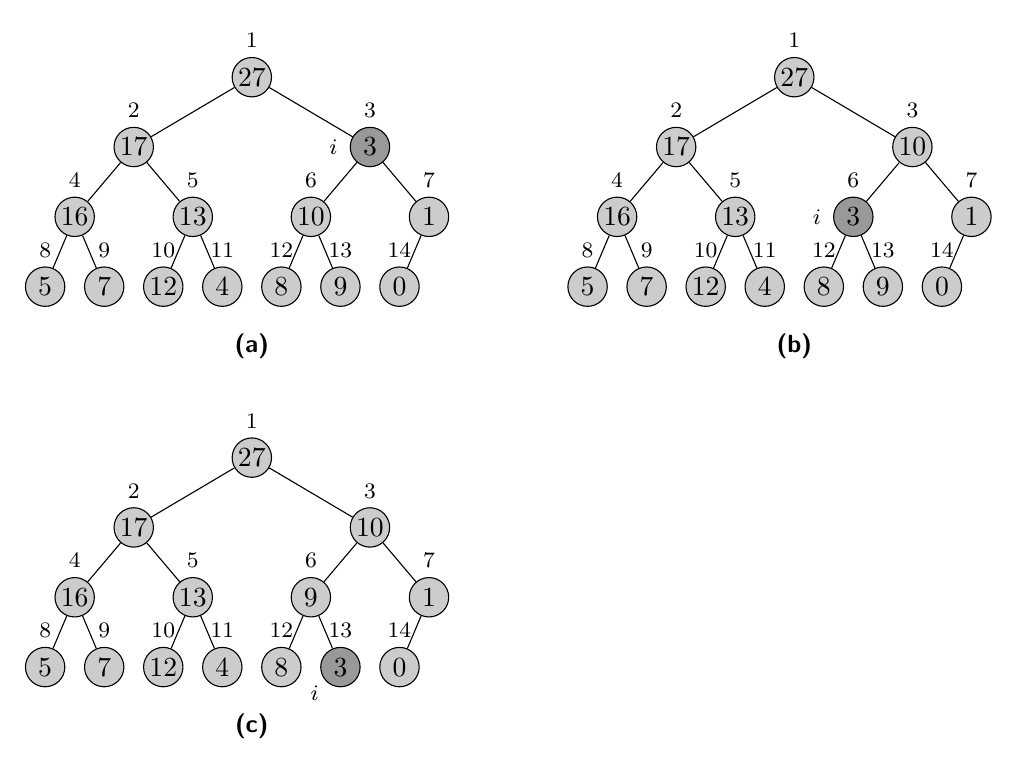
\begin{tikzpicture}[
	pic matrix/.style = {matrix of nodes, column sep=15mm, row sep=5mm, draw=none, fill=none, rectangle},
	level/.style = {level distance=10mm, sibling distance=60mm/2^#1},
	every node/.style = {align=center, inner sep=-1pt, minimum size=5mm, circle, draw, fill=black!20},
	every label/.style = {font=\footnotesize, minimum size=4mm, draw=none, fill=none},
	marked node/.style = {fill=black!40},
	picture label/.style = {font=\small\bfseries\sffamily, draw=none, fill=none}
]

\matrix[pic matrix] (pic) {
	\node[label=1] {27}
		child {node[label=2] {17}
			child {node[label=4] {16}
				child {node[label=8] {5}}
				child {node[label=9] {7}}
			}
			child {node[label=5] {13}
				child {node[label=10] {12}}
				child {node[label=11] (x) {4}}
			}
		}
		child {node[marked node, label=3, label=left:$i$] {3}
			child {node[label=6] {10}
				child {node[label=12] (y) {8}}
				child {node[label=13] {9}}
			}
			child {node[label=7] {1}
				child {node[label=14] {0}}
				child[missing]
			}
		};
	\node[picture label, below=5mm] at ($ (x)!0.5!(y) $) {(a)};
	&
	\node[label=1] {27}
		child {node[label=2] {17}
			child {node[label=4] {16}
				child {node[label=8] {5}}
				child {node[label=9] {7}}
			}
			child {node[label=5] {13}
				child {node[label=10] {12}}
				child {node[label=11] (x) {4}}
			}
		}
		child {node[label=3] {10}
			child {node[marked node, label=6, label=left:$i$] {3}
				child {node[label=12] (y) {8}}
				child {node[label=13] {9}}
			}
			child {node[label=7] {1}
				child {node[label=14] {0}}
				child[missing]
			}
		};
	\node[picture label, below=5mm] at ($ (x)!0.5!(y) $) {(b)};
	\\
	\node[label=1] {27}
		child {node[label=2] {17}
			child {node[label=4] {16}
				child {node[label=8] {5}}
				child {node[label=9] {7}}
			}
			child {node[label=5] {13}
				child {node[label=10] {12}}
				child {node[label=11] (x) {4}}
			}
		}
		child {node[label=3] {10}
			child {node[label=6] {9}
				child {node[label=12] (y) {8}}
				child {node[marked node, label=13, label=below left:{$i$}] {3}}
			}
			child {node[label=7] {1}
				child {node[label=14] {0}}
				child[missing]
			}
		};
	\node[picture label, below=5mm] at ($ (x)!0.5!(y) $) {(c)};
	& \\
};

\end{tikzpicture}

	\caption{Działanie procedury $\proc{Max-Heapify}(A,3)$ dla tablicy $A=\langle$27,\! 17,\! 3,\! 16,\! 13,\! 10,\! 1,\! 5,\! 7,\! 12,\! 4,\! 8,\! 9,\! 0$\rangle$.
{\sffamily\bfseries\doubledash{(a)}{(b)}} Drzewo binarne reprezentujące $A$, w~którym przywracana jest własność kopca typu max, odpowiednio, w~węzłach $i=3$ oraz $i=6$.
{\sffamily\bfseries(c)} Wynikowy kopiec z~przywróconą własnością kopca.} \label{fig:6.2-1}
\end{figure}

\exercise %6.2-2
Poniższy pseudokod prezentuje procedurę przywracania własności kopca typu min.
Ponieważ jedyną modyfikacją w~porównaniu z~procedurą \proc{Max-Heapify} jest zmiana znaków nierówności na przeciwne w~warunkach w~wierszach \ref{li:min-heapify-check1} i~\ref{li:min-heapify-check2}, to czas działania tej procedury jest identyczny z~czasem działania \proc{Max-Heapify}, czyli $\Theta(\lg n)$.
\begin{codebox}
\Procname{$\proc{Min-Heapify}(A,i)$}
\li	$l\gets\proc{Left}(i)$
\li	$r\gets\proc{Right}(i)$
\li	\If $l\le\attrib{A}{heap-size}$ i~$A[l]<A[i]$ \label{li:min-heapify-check1}
\li		\Then $\id{smallest}\gets l$
\li		\Else $\id{smallest}\gets i$
		\End
\li	\If $r\le\attrib{A}{heap-size}$ i~$A[r]<A[\id{smallest}]$ \label{li:min-heapify-check2}
\li		\Then $\id{smallest}\gets r$
		\End
\li	\If $\id{smallest}\ne i$
\li		\Then zamień $A[i]\leftrightarrow A[\id{smallest}]$
\li			$\proc{Min-Heapify}(A,\id{smallest})$
		\End
\end{codebox}

\exercise %6.2-3
Jeśli element $A[i]$ jest większy niż jego synowie, to \id{largest} jest ustawiane na $i$ i~warunek z~wiersza 8 nie jest spełniony.
Procedura zakończy więc działanie, nie dokonując żadnej zamiany elementów.

\exercise %6.2-4
Z~\refExercise{6.1-7} mamy, że element o~indeksie $i>\attrib{A}{heap-size}/2$ jest liściem kopca, czyli nie istnieją jego synowie.
W~dwóch pierwszych wierszach procedury \proc{Max-Heapify} obliczone zostaną wartości przekraczające \attrib{A}{heap-size}, więc zmienna \id{largest} przyjmie wartość $i$.
Warunek w~wierszu 8 będzie więc fałszywy i~natychmiast po jego sprawdzeniu procedura zakończy działanie.

\exercise %6.2-5
Iteracyjna wersja procedury \proc{Max-Heapify} została przedstawiona poniżej.
\begin{codebox}
\Procname{$\proc{Iterative-Max-Heapify}(A,i)$}
\li	\While \const{true}
\li		\Do $l\gets\proc{Left}(i)$ \label{li:iterative-max-heapify-begin}
\li			$r\gets\proc{Right}(i)$
\li			\If $l\le\attrib{A}{heap-size}$ i~$A[l]>A[i]$
\li				\Then $\id{largest}\gets l$
\li				\Else $\id{largest}\gets i$
				\End
\li			\If $r\le\attrib{A}{heap-size}$ i~$A[r]>A[\id{largest}]$
\li				\Then $\id{largest}\gets r$
				\End \label{li:iterative-max-heapify-end}
\li			\If $\id{largest}=i$ \label{li:iterative-max-heapify-cond}
\li				\Then \Return
				\End
\li			zamień $A[i]\leftrightarrow A[\id{largest}]$
\li			$i\gets\id{largest}$
		\End
\end{codebox}
Działania wykonywane w~wierszach \doubledash{\ref{li:iterative-max-heapify-begin}}{\ref{li:iterative-max-heapify-end}} są identyczne jak w~oryginalnej implementacji procedury.
W~zależności od wyniku testu z~wiersza \ref{li:iterative-max-heapify-cond} procedura kończy działanie albo zamienia elementy $A[i]$ i~$A[\id{largest}]$, po czym symuluje wywołanie rekurencyjne, aktualizując wartość zmiennej $i$ i~wykonując kolejną iterację pętli \kw{while}.

\exercise %6.2-6
Najgorszy przypadek dla procedury \proc{Max-Heapify} zachodzi wówczas, gdy zostanie ona wywołana dla korzenia kopca i~schodzi rekurencyjnie aż do jego ostatniego poziomu.
Najdłuższa ścieżka od korzenia do liścia składa się z~$h=\lfloor\lg n\rfloor$ krawędzi (z~\refExercise{6.1-2}) i~tyle będzie wywołań rekurencyjnych procedury w~najgorszym przypadku.
Koszt pracy wykonanej na każdym poziomie rekursji jest stały, a~więc procedura \proc{Max-Heapify} działa wtedy w~czasie $\Omega(\lg n)$.
Przykładowym drzewem, dla którego procedura wykona opisane operacje, jest takie, w~którym korzeń ma wartość 0, a~każdy inny węzeł ma wartość 1.

\subchapter{Budowanie kopca}

\exercise %6.3-1
Ilustracja działania procedury \proc{Build-Max-Heap} dla tablicy $A$ znajduje się na rys.\ \ref{fig:6.3-1}.
\begin{figure}[!ht]
	\centering \begin{tikzpicture}[
	marked node/.style = {tree node, med gray},
	every label/.style = {index node, draw=none, fill=none},
	outer/.append style = {node distance=9mm and 15mm},
	inner/.style = {draw=none, fill=none, node distance=3mm},
]

\node[outer] (pic a) {
\begin{tikzpicture}
	\node[inner] (pic a1) {
	\begin{tikzpicture}[
		row 1/.style = {nodes={light gray}}
	]
		\matrix[array] (arr) {5 & 3 & 17 & 10 & 84 & 19 & 6 & 22 & 9 \\};
		\node[left=of arr-1-1.west] {$A$};
	\end{tikzpicture}
	};
	\node[inner, below=of pic a1] {
	\begin{tikzpicture}[
		every node/.style = {tree node},
		anchor = center
	]
		\node[label=1] {5}
			child {node[label=2] {3}
				child {node[marked node, label=4, label=left:{$i$}] {10}
					child {node[label=8] {22}}
					child {node[label=9] {9}}
				}
				child {node[label=5] {84}}
			}
			child {node[label=3] {17}
				child {node[label=6] {19}}
				child {node[label=7] {6}
					child[missing]
					child {node[draw=none, fill=none] {} edge from parent[draw=none]}
				}
			};
	\end{tikzpicture}
	};
\end{tikzpicture}
};

\node[outer, right=of pic a.south east, anchor=south west] (pic b) {
\begin{tikzpicture}[
	every node/.style = {tree node},
	anchor = center
]
	\node[label=1] {5}
		child {node[label=2] {3}
			child {node[label=4] {22}
				child {node[label=8] {10}}
				child {node[label=9] {9}}
			}
			child {node[label=5] {84}}
		}
		child {node[marked node, label=3, label=left:{$i$}] {17}
			child {node[label=6] {19}}
			child {node[label=7] {6}
				child[missing]
				child {node[draw=none, fill=none] {} edge from parent[draw=none]}
			}
		};
\end{tikzpicture}
};

\node[outer, below=of pic a] (pic c) {
\begin{tikzpicture}[
	every node/.style = {tree node},
	anchor = center
]
	\node[label=1] {5}
		child {node[marked node, label=2, label=left:{$i$}] {3}
			child {node[label=4] {22}
				child {node[label=8] {10}}
				child {node[label=9] {9}}
			}
			child {node[label=5] {84}}
		}
		child {node[label=3] {19}
			child {node[label=6] {17}}
			child {node[label=7] {6}
				child[missing]
				child {node[draw=none, fill=none] {} edge from parent[draw=none]}
			}
		};
\end{tikzpicture}
};

\node[outer, right=of pic c] (pic d) {
\begin{tikzpicture}[
	every node/.style = {tree node},
	anchor = center
]
	\node[marked node, label=1, label=left:{$i$}] {5}
		child {node[label=2] {84}
			child {node[label=4] {22}
				child {node[label=8] {10}}
				child {node[label=9] {9}}
			}
			child {node[label=5] {3}}
		}
		child {node[label=3] {19}
			child {node[label=6] {17}}
			child {node[label=7] {6}
				child[missing]
				child {node[draw=none, fill=none] {} edge from parent[draw=none]}
			}
		};
\end{tikzpicture}
};

\node[outer, below=of pic c] (pic e) {
\begin{tikzpicture}[
	every node/.style = {tree node},
	anchor = center
]
	\node[label=1] {84}
		child {node[label=2] {22}
			child {node[label=4] {10}
				child {node[label=8] {5}}
				child {node[label=9] {9}}
			}
			child {node[label=5] {3}}
		}
		child {node[label=3] {19}
			child {node[label=6] {17}}
			child {node[label=7] {6}
				child[missing]
				child {node[draw=none, fill=none] {} edge from parent[draw=none]}
			}
		};
\end{tikzpicture}
};

\foreach \x in {a,b,c,d,e} {
	\node[subpicture label, below=-3mm of pic \x] {(\x)};
}

\end{tikzpicture}

	\caption{Działanie procedury \proc{Build-Max-Heap} dla tablicy $A=\langle5,3,17,10,84,19,6,22,9\rangle$.
{\sffamily\bfseries(a)} Tablica $A$ i~reprezentowane przez nią drzewo binarne przed pierwszym wywołaniem \proc{Max-Heapify} z~wiersza 3.
{\sffamily\bfseries\doubledash{(b)}{(d)}} Drzewo przed każdym kolejnym wywołaniem \proc{Max-Heapify}.
{\sffamily\bfseries(e)} Wynikowy kopiec typu max.} \label{fig:6.3-1}
\end{figure}

\exercise %6.3-2
Wywołując $\proc{Max-Heapify}(A,i)$, zakładamy, że drzewa o~korzeniach $\proc{Left}(i)$ i~$\proc{Right}(i)$ (o~ile istnieją) są kopcami typu max.
Jeżeli podczas budowy kopca procedura \proc{Max-Heapify} byłaby wywoływana dla węzłów o~rosnących indeksach, to nie moglibyśmy zagwarantować, że założenie to jest spełnione, dlatego przetwarzanie odbywa się w~kolejności malejących indeksów.

\exercise %6.3-3
Oznaczmy kopiec przez $T$, a~przez $n_h$ -- ilość węzłów kopca $T$ znajdujących się na wysokości $h$.
Udowodnimy fakt przez indukcję względem $h$.

W~pierwszym kroku indukcji musimy pokazać, że $n_0\le\lceil n/2\rceil$.
W~rzeczywistości udowodnimy, że $n_0=\lceil n/2\rceil$.
Korzystając z~\refExercise{6.1-7}, mamy, że węzły znajdujące się w~$T$ na wysokości 0, czyli jego liście, zajmują pozycje $\lfloor n/2\rfloor+1\twodots n$.
Jest ich zatem
\[
    n_0 = n-(\lfloor n/2\rfloor+1)+1 = n-\lfloor n/2\rfloor = \lceil n/2\rceil.
\]
A~więc przypadek bazowy indukcji jest spełniony.

Załóżmy teraz, że $h>0$ i~że twierdzenie jest spełnione dla węzłów na wysokości $h-1$.
Ponadto niech $T'$ będzie kopcem powstałym z~$T$ po usunięciu z~niego wszystkich jego liści.
Nowy kopiec ma zatem $n'=n-n_0$ węzłów.
Ponieważ w~kroku bazowym pokazaliśmy, że $n_0=\lceil n/2\rceil$, to stąd $n'=n-\lceil n/2\rceil=\lfloor n/2\rfloor$.
Węzły, które w~kopcu $T$ znajdują się na wysokości $h$, w~$T'$ zajmują wysokość $h-1$, więc jeśli oznaczymy przez $n_{h-1}'$ liczbę węzłów na wysokości $h-1$ w~kopcu $T'$, to wówczas będzie $n_h=n_{h-1}'$.
Wykorzystując założenie indukcyjne, dostajemy
\[
    n_h = n_{h-1}' \le \lceil n'\!/2^h\rceil = \lceil\lfloor n/2\rfloor/2^h\rceil \le \lceil(n/2)/2^h\rceil = \lceil n/2^{h+1}\rceil,
\]
co kończy dowód.

\subchapter{Algorytm sortowania przez kopcowanie (heapsort)}

\exercise %6.4-1
Na rys.\ \ref{fig:6.4-1} zilustrowano działanie sortowania przez kopcowanie dla tablicy $A$.
\begin{figure}[!ht]
	\centering \begin{tikzpicture}[
	marked node/.style = {tree node, fill=black!40},
	every label/.style = {index node, draw=none, fill=none},
	outer/.append style = {node distance=13mm and 8mm},
	outer scaled/.style = {outer, scale=0.7}
]

\node[outer scaled] (pic a) {
\begin{tikzpicture}[
	every node/.style = {tree node},
	anchor = center
]
	\node {25}
		child {node {13}
			child {node {8}
				child {node {5}}
				child {node {4}}
			}
			child {node {7}}
		}
		child {node {20}
			child {node {17}}
			child {node {2}
				child[missing]
				child {node[draw=none, fill=none] {} edge from parent[draw=none]}
			}
		};
\end{tikzpicture}
};

\node[outer scaled, right=of pic a] (pic b) {
\begin{tikzpicture}[
	every node/.style = {tree node},
	anchor = center
]
	\node {20}
		child {node {13}
			child {node {8}
				child {node {5}}
				child {node[marked node, label=right:{$i$}] {25} edge from parent[draw=none]}
			}
			child {node {7}}
		}
		child {node {17}
			child {node {4}}
			child {node {2}
				child[missing]
				child {node[draw=none, fill=none] {} edge from parent[draw=none]}
			}
		};
\end{tikzpicture}
};

\node[outer scaled, right=of pic b] (pic c) {
\begin{tikzpicture}[
	every node/.style = {tree node},
	anchor = center
]
	\node {17}
		child {node {13}
			child {node {8}
				child {node[marked node, label=left:{$i$}] {20} edge from parent[draw=none]}
				child {node[marked node] {25} edge from parent[draw=none]}
			}
			child {node {7}}
		}
		child {node {5}
			child {node {4}}
			child {node {2}
				child[missing]
				child {node[draw=none, fill=none, label=right:{}] {} edge from parent[draw=none]}
			}
		};
\end{tikzpicture}
};

\node[outer scaled, below=of pic a] (pic d) {
\begin{tikzpicture}[
	every node/.style = {tree node},
	anchor = center
]
	\node {13}
		child {node {8}
			child {node {2}
				child {node[marked node] {20} edge from parent[draw=none]}
				child {node[marked node] {25} edge from parent[draw=none]}
			}
			child {node {7}}
		}
		child {node {5}
			child {node {4}}
			child {node[marked node, label=left:{$i$}] {17} edge from parent[draw=none]
				child[missing]
				child {node[draw=none, fill=none] {} edge from parent[draw=none]}
			}
		};
\end{tikzpicture}
};

\node[outer scaled, below=of pic b] (pic e) {
\begin{tikzpicture}[
	every node/.style = {tree node},
	anchor = center
]
	\node {8}
		child {node {7}
			child {node {2}
				child {node[marked node] {20} edge from parent[draw=none]}
				child {node[marked node] {25} edge from parent[draw=none]}
			}
			child {node {4}}
		}
		child {node {5}
			child {node[marked node, label=left:{$i$}] {13} edge from parent[draw=none]}
			child {node[marked node] {17} edge from parent[draw=none]
				child[missing]
				child {node[draw=none, fill=none] {} edge from parent[draw=none]}
			}
		};
\end{tikzpicture}
};

\node[outer scaled, below=of pic c] (pic f) {
\begin{tikzpicture}[
	every node/.style = {tree node},
	anchor = center
]
	\node {7}
		child {node {4}
			child {node {2}
				child {node[marked node] {20} edge from parent[draw=none]}
				child {node[marked node] {25} edge from parent[draw=none]}
			}
			child {node[marked node, label=left:{$i$}] {8} edge from parent[draw=none]}
		}
		child {node {5}
			child {node[marked node] {13} edge from parent[draw=none]}
			child {node[marked node] {17} edge from parent[draw=none]
				child[missing]
				child {node[draw=none, fill=none] {} edge from parent[draw=none]}
			}
		};
\end{tikzpicture}
};

\node[outer scaled, below=of pic d] (pic g) {
\begin{tikzpicture}[
	every node/.style = {tree node},
	anchor = center
]
	\node {5}
		child {node {4}
			child {node[marked node, label=left:{$i$}] {7} edge from parent[draw=none]
				child {node[marked node] {20} edge from parent[draw=none]}
				child {node[marked node] {25} edge from parent[draw=none]}
			}
			child {node[marked node] {8} edge from parent[draw=none]}
		}
		child {node {2}
			child {node[marked node] {13} edge from parent[draw=none]}
			child {node[marked node] {17} edge from parent[draw=none]
				child[missing]
				child {node[draw=none, fill=none] {} edge from parent[draw=none]}
			}
		};
\end{tikzpicture}
};

\node[outer scaled, below=of pic e] (pic h) {
\begin{tikzpicture}[
	every node/.style = {tree node},
	anchor = center
]
	\node {4}
		child {node {2}
			child {node[marked node] {7} edge from parent[draw=none]
				child {node[marked node] {20} edge from parent[draw=none]}
				child {node[marked node] {25} edge from parent[draw=none]}
			}
			child {node[marked node] {8} edge from parent[draw=none]}
		}
		child {node[marked node, label=left:{$i$}] {5} edge from parent[draw=none]
			child {node[marked node] {13} edge from parent[draw=none]}
			child {node[marked node] {17} edge from parent[draw=none]
				child[missing]
				child {node[draw=none, fill=none] {} edge from parent[draw=none]}
			}
		};
\end{tikzpicture}
};

\node[outer scaled, below=of pic f] (pic i) {
\begin{tikzpicture}[
	every node/.style = {tree node},
	anchor = center
]
	\node {2}
		child {node[marked node, label=left:{$i$}] {4} edge from parent[draw=none]
			child {node[marked node] {7} edge from parent[draw=none]
				child {node[marked node] {20} edge from parent[draw=none]}
				child {node[marked node] {25} edge from parent[draw=none]}
			}
			child {node[marked node] {8} edge from parent[draw=none]}
		}
		child {node[marked node] {5} edge from parent[draw=none]
			child {node[marked node] {13} edge from parent[draw=none]}
			child {node[marked node] {17} edge from parent[draw=none]
				child[missing]
				child {node[draw=none, fill=none] {} edge from parent[draw=none]}
			}
		};
\end{tikzpicture}
};

\node[outer, below=of pic g] (pic j) {
\begin{tikzpicture}[
	row 1/.style = {nodes={fill=black!20}}
]
	\matrix[array] (arr) {2 & 4 & 5 & 7 & 8 & 13 & 17 & 20 & 25 \\};
	\node[left=3mm of arr-1-1] {$A$};
\end{tikzpicture}
};

\foreach \x in {a,b,c,d,e,f,g,h,i,j} {
	\node[subpicture label, below=2mm of pic \x] {(\x)};
}

\end{tikzpicture}

	\caption{Działanie procedury \proc{Heapsort} dla tablicy $A=\langle5,13,2,25,7,17,20,8,4\rangle$.
{\sffamily\bfseries(a)} Kopiec zaraz po jego zbudowaniu przez \proc{Build-Max-Heap}.
{\sffamily\bfseries\doubledash{(b)}{(i)}} Kopiec i~elementy z~niego usunięte po każdym wywołaniu \proc{Max-Heapify} w~wierszu 5.
{\sffamily\bfseries(j)} Wynikowa posortowana tablica.} \label{fig:6.4-1}
\end{figure}

\exercise %6.4-2
Pokażemy, że podany niezmiennik jest spełniony przed pierwszą iteracją pętli \kw{for}, że każda iteracja tej pętli zachowuje niezmiennik i~że po zakończeniu pętli z~niezmiennika można wywnioskować poprawność procedury.
\begin{description}
	\item[Inicjowanie:] Przed pierwszą iteracją pętli mamy $i=\attrib{A}{length}=n$.
Wówczas fragment $A[1\twodots i]$ jest całą tablicą $A$, która stanowi kopiec typu max, utworzony w~wyniku działania procedury \proc{Build-Max-Heap}, natomiast fragment $A[i+1\twodots n]$ jest pusty.
	\item[Utrzymanie:] Załóżmy, że niezmiennik jest prawdziwy przed wykonaniem kolejnej iteracji pętli.
Podtablica $A[1\twodots i]$ tworzy więc kopiec typu max, którego korzeniem jest $A[1]$, czyli największy element w~tej podtablicy.
Po wykonaniu wiersza 3 znajdzie się on na pozycji $i$.
Dekrementacja \attrib{A}{heap-size} powoduje, że element $A[i]$ nie wchodzi teraz w~skład kopca, ale podtablica $A[i\twodots n]$ zawiera teraz $n-i+1$ największych elementów z~$A[1\twodots n]$ posortowanych niemalejąco, ponieważ element $A[i]$ jest równy lub mniejszy od wcześniej umieszczonych tam elementów.
W~tym momencie korzeń może naruszać własność kopca typu max, dlatego w~wierszu 5 zostaje wywołana dla niego procedura \proc{Max-Heapify} przywracająca tę własność.
Uaktualnienie $i$ powoduje odtworzenie niezmiennika.
	\item[Zakończenie:] Po zakończeniu działania pętli jest $i=1$, zatem podtablica $A[1\twodots i]$ składa się z~jednego elementu, który jest najmniejszym elementem tablicy $A$.
Ponadto $n-1$ pozostałych elementów jest uszeregowanych w~kolejności niemalejącej w~podtablicy $A[2\twodots n]$.
Stąd mamy, że tablica $A$ jest posortowana.
\end{description}

\exercise %6.4-3
Na podstawie analizy zamieszczonej w~Podręczniku czasem działania algorytmu heapsort dla tablicy o~rozmiarze $n$ jest $O(n\lg n)$.
Z~\refExercise{6.4-5} mamy, że jest to w~rzeczywistości oszacowanie dokładne.
A~zatem w~szczególności dla tablicy posortowanej rosnąco i~tablicy posortowanej malejąco heapsort działa w~czasie $\Theta(n\lg n)$.

\exercise %6.4-4
Przypadek pesymistyczny algorytmu heapsort ma miejsce wtedy, gdy każde wywołanie \proc{Max-Heapify} z~wiersza 5 schodzi rekurencyjnie aż do ostatniego poziomu drzewa.
Na mocy wyniku z~\refExercise{6.2-6} oraz wzoru (3.18) wywołania te zabierają łącznie czas
\[
	\sum_{i=2}^n\Omega(\lg i) = \Omega(\lg(n!)) = \Omega(n\lg n)
\]
i~taki jest też czas działania algorytmu heapsort w~pesymistycznym przypadku.

\exercise %6.4-5
Dokonamy analizy liczby wykonywanych instrukcji z~linii 9 procedury \proc{Max-Heapify} podczas działania algorytmu sortowania przez kopcowanie w~przypadku optymistycznym.

Załóżmy, że algorytm heapsort działa na tablicy $A$ o~rozmiarze $n=2^{h+1}-1$, gdzie $h$ jest dodatnią liczbą całkowitą.
A~zatem kopiec zbudowany z~$A$ stanowi pełne drzewo binarne o~wysokości $h$.
Rozważanie tylko takich kopców nie powoduje zmniejszenia ogólności analizy.
Przez \singledash{$j$}{ty} etap działania algorytmu heapsort, gdzie $j=0$, 1, \dots, $h-1$, będziemy rozumieć działania wykonywane podczas iteracji pętli \kw{for} z~procedury \proc{Heapsort}, w~których $2^{h-j}\le i\le2^{h-j+1}-1$.
Inaczej mówiąc, \singledash{$j$}{ty} etap pozbawia kopiec \singledash{$(h-j)$}{tego} poziomu.

\medskip
\noindent\textsf{\textbf{Lemat.}} \textit{Podczas\/ \singledash{$j$}{tego} etapu działania algorytmu heapsort na kopcu\/ $A$ o~rozmiarze\/ $n=2^{h+1}-1$,\/ $h\ge5$, którego wszystkie elementy są różne, liczba wykonanych zamian elementów w~linii 9 procedury \proc{Max-Heapify} jest większa niż\/ $(h-j-5)2^{h-j-3}$.}
\begin{proof}
Oznaczmy przez $m_j$ badaną liczbę zamian elementów wykonywanych w~\singledash{$j$}{tym} etapie.
Niech $j=0$ i~bez utraty ogólności załóżmy, że $\langle A[1],A[2],\dots,A[n]\rangle$ jest permutacją $\langle1,2,\dots,n\rangle$.
Liczbę $k$ będziemy nazywać \textbf{dużą}, jeśli $k\ge(n+1)/2$.
Niech $S$ będzie zbiorem indeksów dużych elementów w~kopcu $A$, które nie są liśćmi, czyli
\[
    S = \biggl\{\,i\in\Bigl\{1,2,\dots,\frac{n-1}{2}\Bigr\}:A[i]\ge\frac{n+1}{2}\,\biggr\}.
\]
Zauważmy, że wszystkie elementy, których pozycjami w~$A$ są indeksy ze zbioru $S$, zostaną usunięte z~kopca w~etapie $j=0$.
A~zatem muszą wpierw znaleźć się w~korzeniu kopca za sprawą wykonania pewnej liczby zamian z~linii 9 procedury \proc{Max-Heapify}.
Stąd $m_0$ spełnia nierówność
\[
    m_0 \ge \sum_{i\in S}d_i,
\]
gdzie $d_i$ oznacza głębokość węzła o~początkowej pozycji $i$ w~kopcu $A$.

Węzły o~indeksach ze zbioru $S$ tworzą w~kopcu $A$ poddrzewo $T$ o~korzeniu w~$A[1]$.
Jest tak dlatego, że jeśli węzeł $A[i]$ jest duży, to $A[\proc{Parent}(i)]$ również jest duży, a~więc także wszystkie węzły na ścieżce od $A[i]$ do korzenia kopca, czyli $A[1]$.
Jeśli zastąpimy każde puste poddrzewo w~$T$ pojedynczym węzłem, to dostaniemy regularne drzewo binarne, którego długość ścieżki wewnętrznej (patrz \refExercise{B.5-5}) wynosi $m_0$.
W~zbiorze wszystkich drzew binarnych o~$|S|$ węzłach wewnętrznych najmniejsza możliwa długość ścieżki wewnętrznej jest osiągana dla pełnego drzewa binarnego (przy czym ostatni poziom tego drzewa może nie być wypełniony) i~wynosi $\sum_{k=1}^{|S|}\lfloor\lg k\rfloor$.
Korzystając ze wzoru (3.3) i~\refExercise{8.1-2}, mamy
\[
    m_0 \ge \sum_{k=1}^{|S|}\lfloor\lg k\rfloor > \sum_{k=1}^{|S|}(\lg k-1) = \sum_{k=1}^{|S|}\lg k-|S| \ge \frac{|S|}{2}\lg\frac{|S|}{2}-|S| = \frac{|S|}{2}\lg|S|-\frac{3}{2}|S|.
\]

Pokażemy teraz, że $|S|\ge2^{h-2}$.
Rozważmy w~tym celu permutację $\pi$ elementów kopca $A$ na początku zerowego etapu w~kolejności ich odwiedzania podczas przechodzenia kopca metodą inorder.
Jeśli $\pi(i)$, gdzie $i\ge2$, jest liściem kopca, to $\pi(i-1)$ nie może być liściem kopca.
Jeśli w~dodatku $\pi(i)$ jest dużym liściem, to $\pi(i-1)$ jest dużym węzłem wewnętrznym.
Stąd indeks elementu $\pi(i-1)$ należy do $S$.
Mamy więc, że $l$ -- liczba dużych liści -- nie przekracza $|S|+1$, nawet jeśli $\pi(1)$ jest dużym liściem.
Ponieważ liczba dużych elementów w~kopcu wynosi $(n+1)/2=2^h$, to otrzymujemy, że $|S|=2^h-l\ge2^h-(|S|+1)$, skąd $|S|\ge2^{h-1}-1/2\ge2^{h-2}$.

Powracając teraz do oszacowania na $m_0$, mamy
\[
    m_0 > \frac{|S|}{2}\lg|S|-\frac{3}{2}|S| = \frac{|S|}{2}(\lg|S|-3) \ge 2^{h-3}(h-5),
\]
czyli lemat jest prawdziwy, gdy $j=0$.

Na początku \singledash{$j$}{tego} etapu kopiec ma wysokość $h-j$, więc dowód lematu dla \singledash{$j$}{tego} etapu, gdzie $1\le j\le h-1$, sprowadza się do dowodu oszacowania $m_0$ dla kopca o~rozmiarze $n=2^{h-j+1}-1$.
\end{proof}

Załóżmy teraz, że $h\ge5$ i~wykorzystajmy oznaczenie $m_j$ z~powyższego dowodu.
Sumaryczną liczbę zamian elementów podczas sortowania $n$ liczb, na podstawie lematu, ograniczamy od dołu:
\[
    \sum_{j=0}^{h-1}m_j > \sum_{j=0}^{h-5}m_j > \sum_{j=0}^{h-5}(h-j-5)2^{h-j-3} = \sum_{j=0}^{h-5}j2^{j+2} = 4\sum_{j=0}^{h-5}j2^j.
\]
Ostatnią sumę obliczamy poprzez skorzystanie ze wzoru (A.5):
\[
    \sum_{j=0}^{h-5}jx^j = x\cdot\frac{d}{dx}\biggl(\sum_{j=0}^{h-5}x^j\biggr) = x\cdot\frac{d}{dx}\biggl(\frac{x^{h-4}-1}{x-1}\biggr) = x\,\frac{(h-4)x^{h-5}(x-1)-(x^{h-4}-1)}{(x-1)^2}.
\]
Przyjmując teraz $x=2$ i~korzystając z~nierówności $2^h>n/2$ i~$h>\lg n-1$, mamy ostatecznie
\[
    4\sum_{j=0}^{h-5}j2^j = (h-4)2^{h-2}-2^{h-1}+8 > (h-6)2^{h-2} > \frac{1}{8}n\lg n-\frac{7}{8}n = \Omega(n\lg n).
\]
Otrzymany wynik stanowi oszacowanie czasu działania algorytmu heapsort w~przypadku optymistycznym.

\subchapter{Kolejki priorytetowe}

\exercise %6.5-1
Na rys.\ \ref{fig:6.5-1} został przedstawiony kopiec wejściowy $A$ i~wynikowy kopiec otrzymany w~wyniku działania procedury \proc{Heap-Extract-Max}.
W~wierszu 3 zmiennej \id{max} przypisywana jest maksymalna wartość kopca, czyli 15.
Następnie korzeń otrzymuje wartość 1 i~rozmiar kopca jest pomniejszany o~1.
Po przywróceniu własności kopca w~linii 6 procedura zwraca wartość \id{max}.
\begin{figure}[!ht]
	\centering \begin{tikzpicture}

\node[outer] (pic a) {
\begin{tikzpicture}[
	every node/.style = {tree node},
	anchor = center
]
	\node {15}
		child {node {13}
			child {node {5}
				child {node {4}}
				child {node {0}}
			}
			child {node {12}
				child {node {6}}
				child {node {2}}
			}
		}
		child {node {9}
			child {node {8}
				child {node {1}}
				child[missing]
			}
			child {node {7}
				child[missing]
				child {node[draw=none, fill=none] {} edge from parent[draw=none]}
			}
		};
\end{tikzpicture}
};

\node[outer, right=15mm of pic a] (pic b) {
\begin{tikzpicture}[
	every node/.style = {tree node},
	anchor = center
]
	\node {13}
		child {node {12}
			child {node {5}
				child {node {4}}
				child {node {0}}
			}
			child {node {6}
				child {node {1}}
				child {node {2}}
			}
		}
		child {node {9}
			child {node {8}}
			child {node {7}
				child[missing]
				child {node[draw=none, fill=none] {} edge from parent[draw=none]}
			}
		};
\end{tikzpicture}
};

\node[subpicture label, below=2mm of pic a] {(a)};
\node[subpicture label, below=2mm of pic b] {(b)};

\end{tikzpicture}

	\caption{Działanie procedury \proc{Heap-Extract-Max} dla kopca $A=\langle15,13,9,5,12,8,7,4,0,6,2,1\rangle$.
{\sffamily\bfseries(a)} Kopiec wejściowy $A$.
{\sffamily\bfseries(b)} Kopiec $A$ po usunięciu maksymalnej wartości i~przywróceniu własności kopca naruszonej przez korzeń, któremu wcześniej przypisano wartość 1.} \label{fig:6.5-1}
\end{figure}

\exercise %6.5-2
Procedura \proc{Max-Heap-Insert} rozpoczyna działanie od dodania do kopca nowego elementu o~wartości $-\infty$.
Wartość ta jest następnie odpowiednio modyfikowana i~element jest umieszczany w~odpowiednim miejscu w~kopcu dzięki wywołaniu \proc{Heap-Increase-Key}.
Działanie procedury $\proc{Max-Heap-Insert}(A,10)$ zostało przedstawione na rys.\ \ref{fig:6.5-2}.
\begin{figure}[!ht]
	\centering \begin{tikzpicture}[
	marked node/.style = {tree node, fill=black!40},
	every label/.style = {index node, draw=none, fill=none}
]

\node[outer] (pic a) {
\begin{tikzpicture}[
	every node/.style = {tree node},
	anchor = center
]
	\node {15}
		child {node {13}
			child {node {5}
				child {node {4}}
				child {node {0}}
			}
			child {node {12}
				child {node {6}}
				child {node {2}}
			}
		}
		child {node {9}
			child {node {8}
				child {node {1}}
				child {node[marked node, font=\footnotesize] {$-\infty$}}
			}
			child {node {7}
				child[missing]
				child {node[draw=none, fill=none] {} edge from parent[draw=none]}
			}
		};
\end{tikzpicture}
};

\node[outer, right=of pic a] (pic b) {
\begin{tikzpicture}[
	every node/.style = {tree node},
	anchor = center
]
	\node {15}
		child {node {13}
			child {node {5}
				child {node {4}}
				child {node {0}}
			}
			child {node {12}
				child {node {6}}
				child {node {2}}
			}
		}
		child {node {9}
			child {node {8}
				child {node {1}}
				child {node[marked node, font=\footnotesize, label=right:{$i$}] {10}}
			}
			child {node {7}
				child[missing]
				child {node[draw=none, fill=none] {} edge from parent[draw=none]}
			}
		};
\end{tikzpicture}
};

\node[outer, below=15mm of pic a] (pic c) {
\begin{tikzpicture}[
	every node/.style = {tree node},
	anchor = center
]
	\node {15}
		child {node {13}
			child {node {5}
				child {node {4}}
				child {node {0}}
			}
			child {node {12}
				child {node {6}}
				child {node {2}}
			}
		}
		child {node {9}
			child {node[marked node, font=\footnotesize, label=right:{$i$}] {10}
				child {node {1}}
				child {node {8}}
			}
			child {node {7}
				child[missing]
				child {node[draw=none, fill=none] {} edge from parent[draw=none]}
			}
		};
\end{tikzpicture}
};

\node[outer, right=of pic c] (pic d) {
\begin{tikzpicture}[
	every node/.style = {tree node},
	anchor = center
]
	\node {15}
		child {node {13}
			child {node {5}
				child {node {4}}
				child {node {0}}
			}
			child {node {12}
				child {node {6}}
				child {node {2}}
			}
		}
		child {node[marked node, font=\footnotesize, label=right:{$i$}] {10}
			child {node {9}
				child {node {1}}
				child {node {8}}
			}
			child {node {7}
				child[missing]
				child {node[draw=none, fill=none] {} edge from parent[draw=none]}
			}
		};
\end{tikzpicture}
};

\node[subpicture label, below=2mm of pic a] {(a)};
\node[subpicture label, below=2mm of pic b] {(b)};
\node[subpicture label, below=2mm of pic c] {(c)};
\node[subpicture label, below=2mm of pic d] {(d)};

\end{tikzpicture}

	\caption{Działanie procedury $\proc{Max-Heap-Insert}(A,10)$ dla kopca $A=\langle$15,\! 13,\! 9,\! 5,\! 12,\! 8,\! 7,\! 4,\! 0,\! 6,\! 2,\! 1$\rangle$.
{\sffamily\bfseries(a)} Kopiec po dodaniu nowego elementu o~wartości początkowej $-\infty$.
{\sffamily\bfseries(b)} Działa teraz procedura \proc{Heap-Increase-Key}.
Na rysunku pokazano wartość zmiennej $i$ w~tej procedurze.
Wartość nowego elementu została zwiększona i~wynosi teraz 10.
{\sffamily\bfseries(c)} Po wykonaniu pierwszej iteracji pętli \kw{while} procedury \proc{Heap-Increase-Key} nowy element został zamieniony ze swoim ojcem.
{\sffamily\bfseries(d)} Po drugiej iteracji pętli nastąpiła jeszcze jedna zamiana nowego elementu i~jego aktualnego ojca, dzięki czemu $A$ spełnia już własność kopca i~procedura kończy działanie.} \label{fig:6.5-2}
\end{figure}

\exercise %6.5-3
Zakładamy, że tablica $A$ stanowi kopiec typu min.
Poniższe procedury stanowią implementację kolejki priorytetowej typu min i~działają analogicznie do odpowiadających im procedur dla kolejki priorytetowej typu max.
\begin{codebox}
\Procname{$\proc{Heap-Minimum}(A)$}
\li	\Return $A[1]$
\end{codebox}
\begin{codebox}
\Procname{$\proc{Heap-Extract-Min}(A)$}
\li	\If $\attrib{A}{heap-size}<1$
\li		\Then \Error ,,kopiec pusty''
		\End
\li	$\id{min}\gets A[1]$
\li	$A[1]\gets A[\attrib{A}{heap-size}]$
\li	$\attrib{A}{heap-size}\gets\attrib{A}{heap-size}-1$
\li	$\proc{Min-Heapify}(A,1)$
\li	\Return \id{min}
\end{codebox}
\begin{codebox}
\Procname{$\proc{Heap-Decrease-Key}(A,i,\id{key})$}
\li	\If $\id{key}>A[i]$
\li		\Then \Error ,,nowy klucz jest większy niż klucz aktualny''
		\End
\li	$A[i]\gets\id{key}$
\li	\While $i>1$ i~$A[\proc{Parent}(i)]>A[i]$
\li		\Do zamień $A[i]\leftrightarrow A[\proc{Parent}(i)]$
\li			$i\gets\proc{Parent}(i)$
		\End
\end{codebox}
\begin{codebox}
\Procname{$\proc{Min-Heap-Insert}(A,\id{key})$}
\li	$\attrib{A}{heap-size}\gets\attrib{A}{heap-size}+1$
\li	$A[\attrib{A}{heap-size}]\gets\infty$
\li	$\proc{Heap-Decrease-Key}(A,\attrib{A}{heap-size},\id{key})$
\end{codebox}

\exercise %6.5-4
Po wykonaniu wiersza 1 procedury \proc{Max-Heap-Insert} wartość $A[\attrib{A}{heap-size}]$ pozostaje niezdefiniowana i~może zawierać liczbę większą niż \id{key}.
Wówczas jednak wywołanie \proc{Heap-Increase-Key} zakończy się z~błędem.
Radzimy sobie z~tym problemem poprzez nadanie elementowi wartości $-\infty$.

\exercise %6.5-5
Dowodzimy, że niezmiennik spełniony jest przed każdą iteracją pętli \kw{while} oraz że po zakończeniu tej pętli z~niezmiennika wynika, że procedura jest poprawna.
\begin{description}
	\item[Inicjowanie:] Przed wykonaniem wiersza 3 tablica $A[1\twodots\attrib{A}{heap-size}]$ jest kopcem typu max.
Zwiększenie wartości $A[i]$ może naruszyć własność kopca tylko dla elementów $A[i]$ oraz $A[\proc{Parent}(i)]$.
	\item[Utrzymanie:] Dokonując zamiany elementów w~wierszu 5 w~bieżącej iteracji pętli, przywracamy własność kopca dla elementów $A[i]$ oraz $A[\proc{Parent}(i)]$.
Jednak operacja ta może wygenerować nową parę elementów niespełniających własności kopca: $A[\proc{Parent}(i)]$ oraz $A[\proc{Parent}(\proc{Parent}(i))]$.
Aktualizacja wartości $i$ powoduje zachowanie niezmiennika, albowiem nowa para elementów jest jedyną, która może naruszać własność kopca.
	\item[Zakończenie:] Pętla kończy działanie, gdy $i\le1$ lub $A[\proc{Parent}(i)]\ge A[i]$.
W~pierwszym przypadku $\proc{Parent}(i)\le0$, co jest niepoprawną wartością dla indeksów tablicy $A$.
W~drugim natomiast jedyna para, która mogłaby naruszać własność kopca, w~rzeczywistości ją spełnia.
A~zatem po zakończeniu wykonywania pętli tablica $A[1\twodots\attrib{A}{heap-size}]$ stanowi kopiec typu max.
\end{description}
Z~prawdziwości niezmiennika pętli wynika, że procedura \proc{Heap-Increase-Key} poprawnie zwiększa wartość węzła $i$, pozostawiając kopiec typu max.

\exercise %6.5-6
Kolejkę FIFO implementujemy, wykorzystując do tego celu kolejkę priorytetową typu min.
Przyjmiemy, że elementy kolejki oprócz kluczy zawierają też dodatkowe dane, natomiast klucze będą odpowiednio modyfikowane tak, aby symulować działanie kolejki FIFO.
Podczas inicjalizacji kolejki ustawimy dodatkowy jej atrybut \id{rank} na 1.
Przed dodaniem nowego elementu do kolejki FIFO ustawimy jego klucz na aktualną wartość pola \id{rank}, następnie wstawimy element do kolejki priorytetowej procedurą \proc{Min-Heap-Insert}, po czym zwiększymy wartość pola \id{rank} o~1.
Z~kolei usuwanie elementów sprowadza się do zwykłego wywołania procedury \proc{Heap-Extract-Min}.
Taka implementacja operacji kolejki FIFO zapewnia, że w~danym momencie w~strukturze danych nie będzie dwóch różnych elementów z~tym samym kluczem i~elementy pobierane będą w~odpowiedniej kolejności.

Realizacja stosu jest podobna, ale używamy do tego celu kolejki priorytetowej typu max.
Podczas wstawiania elementów na stos korzystamy z~procedury \proc{Max-Heap-Insert} i~inkrementujemy jego pole \id{rank} (zainicjalizowane na 1 w~momencie utworzenia stosu).
Usuwanie polega na odnalezieniu i~pobraniu elementu z~największym kluczem, co realizowane jest za pomocą \proc{Heap-Extract-Max}.
W~wyniku tego elementy pobierane są w~kolejności odwrotnej do tej, w~której były wstawiane.

\exercise %6.5-7
\note{Zmienimy nazwę operacji z~sugerowanej w~Podręczniku \proc{Heap-Delete} na \proc{Max-Heap-Delete}, aby odróżnić ją od analogicznej procedury dla kopca typu min.}

\noindent Przedstawiona poniżej procedura \proc{Max-Heap-Delete} zamienia element $A[i]$ w~\singledash{$n$}{elementowym} kopcu $A$ typu max z~jego liściem $A[\attrib{A}{heap-size}]$, po czym dekrementuje \attrib{A}{heap-size}.
Po tym kroku własność kopca może być naruszona przez węzeł $A[i]$ na dwa sposoby.
W~pierwszym przypadku mamy sytuację, w~której $A[i]<A[\proc{Left}(i)]$ lub $A[i]<A[\proc{Right}(i)]$ -- przywracamy więc własność kopca za pomocą wywołania \proc{Max-Heapify}.
W~drugim przypadku $A[i]>A[\proc{Parent}(i)]$, więc w~celu odbudowy struktury kopca wystarczy wykonać podobne operacje, jak w~procedurze \proc{Heap-Increase-Key}.
Ostatni krok procedury to zwrócenie elementu, który początkowo zajmował w~kopcu pozycję $i$.
\begin{codebox}
\Procname{$\proc{Max-Heap-Delete}(A,i)$}
\li	zamień $A[i]\leftrightarrow A[\attrib{A}{heap-size}]$
\li	$\attrib{A}{heap-size}\gets\attrib{A}{heap-size}-1$
\li	$\proc{Max-Heapify}(A,i)$ \label{li:max-heap-delete-heapify}
\li	\While $i>1$ i~$A[\proc{Parent}(i)]<A[i]$ \label{li:max-heap-delete-while-begin}
\li		\Do zamień $A[i]\leftrightarrow A[\proc{Parent}(i)]$
\li			$i\gets\proc{Parent}(i)$
		\End \label{li:max-heap-delete-while-end}
\li	\Return $A[\attrib{A}{heap-size}+1]$
\end{codebox}

Zarówno wywołanie z~wiersza \ref{li:max-heap-delete-heapify}, jak i~pętla \kw{while} w~wierszach \doubledash{\ref{li:max-heap-delete-while-begin}}{\ref{li:max-heap-delete-while-end}} zajmuje czas $O(\lg n)$, a~więc czasem działania procedury \proc{Max-Heap-Delete} jest również $O(\lg n)$.

\exercise %6.5-8
W~algorytmie wykorzystamy kolejkę priorytetową typu min jako strukturę pomocniczą.
Na początku do kolejki zostaną przeniesione elementy z~głowy każdej listy.
Jest oczywiste, że wśród tych elementów znajduje się najmniejszy element listy wynikowej.
Aby go uzyskać, wystarczy wywołać na kolejce operację \proc{Extract-Min}.
Kolejnego elementu należy szukać wśród aktualnych węzłów kolejki lub w~głowie listy, do której początkowo należało usunięte przed chwilą minimum.
Głowę tej listy, o~ile istnieje, przenosimy do kolejki.
W~kolejnych iteracjach powtarzamy te operacje -- pobieramy najmniejszy element kolejki i~wstawiamy na listę wynikową, po czym uzupełniamy kolejkę głową listy, do której należał pobrany element, o~ile lista ta nie jest jeszcze pusta.
Proces ten powtarzamy aż do opróżnienia kolejki, co następuje po przetworzeniu zawartości wszystkich list.
Aby zachować kolejność niemalejącą na liście wynikowej, musimy wstawiać elementy na jej koniec, pamiętając wskaźnik do ogona tej listy.

Podczas działania algorytmu wykonamy $n$ razy operację wstawienia węzła do kolejki zawierającej co najwyżej $k$ elementów i~tyleż samo operacji \proc{Extract-Min}.
Otrzymujemy zatem górne oszacowanie $O(n\lg k)$ na czas działania algorytmu, przy założeniu, że kolejka priorytetowa została zaimplementowana w~oparciu o~kopiec typu min.


\problems

\problem{Budowa kopca przez wstawianie} %6-1

\subproblem %6-1(a)
Procedury te nie zawsze generują identyczne kopce dla tej samej tablicy wejściowej.
Jeśli na przykład rozważymy tablicę $A=\langle1,2,3\rangle$, to kopce budowane przez obie procedury różnią się, jak to widać na rys.\ \ref{fig:6-1(a)}.
\begin{figure}[ht]
	\begin{center}
		\includegraphics{fig_6-1.a}
	\end{center}
	\caption{Porównanie kopców budowanych przez obie procedury dla tablicy $A=\langle1,2,3\rangle$.
{\sffamily\bfseries(a)} Wynik działania \proc{Build-Max-Heap}.
{\sffamily\bfseries(b)} Wynik działania \proc{Build-Max-Heap}$'$.} \label{fig:6-1(a)}
\end{figure}

\subproblem %6-1(b)
Najgorszym przypadkiem dla procedury \proc{Build-Max-Heap}$'$ jest tablica uporządkowana rosnąco.
W~każdym z~$n-1$ wywołań \proc{Max-Heap-Insert} z~wiersza 3 nowy węzeł transportowany jest wówczas aż do korzenia kopca, co wymaga $\Theta(\lg i)$ operacji przy \singledash{$i$}{elementowym} kopcu.
Stąd czas działania \proc{Build-Max-Heap}$'$ w~przypadku pesymistycznym wynosi
\[
	\sum_{i=1}^{n-1}\Theta(\lg i) = \Theta(\lg(n!)) = \Theta(n\lg n).
\]

\problem{Analiza kopców rzędu $d$} %6-2

\subproblem %6-2(a)
\singledash{$d$}{kopiec} będziemy reprezentować w~tablicy w~następujący sposób.
Podobnie jak w~reprezentacji tablicowej kopców binarnych tablica $A$ reprezentująca \singledash{$d$}{kopiec} będzie mieć atrybuty \attrib{A}{length} oraz \attrib{A}{heap-size}.
Na pierwszej pozycji tablicy znajdzie się korzeń kopca, a~pozycje $2\twodots d+1$ będą zajmowane przez $d$ synów korzenia.
Synowie pierwszego z~lewej syna korzenia zajmą pozycje $d+2\twodots2d+1$, synowie drugiego od lewej syna korzenia -- pozycje $2d+2\twodots3d+1$ itd.
Ogólnie, mając dany indeks węzła $i$, można wyznaczyć indeks jego ojca, korzystając ze wzoru $\lceil(i-1)/d\rceil$.
Uogólnienie procedury \proc{Parent} dla kopca rzędu $d$ wygląda zatem następująco:
\begin{codebox}
\Procname{$\proc{Multiary-Parent}(d,i)$}
\zi	\Return $\lceil(i-1)/d\rceil$
\end{codebox}

Łatwo pokazać, że indeks \singledash{$k$}{tego} od lewej syna węzła o~indeksie $i$, gdzie $k=1$, 2, \dots, $d$, jest opisany wzorem $d(i-1)+k+1$.
Poniższa procedura stanowi uogólnienie procedur \proc{Left} i~\proc{Right} dla kopca rzędu $d$ -- w~porównaniu do nich przyjmuje dodatkowy parametr $k$ oznaczający numer szukanego syna węzła $i$.
\begin{codebox}
\Procname{$\proc{Multiary-Child}(d,k,i)$}
\zi	\Return $d(i-1)+k+1$
\end{codebox}

Można sprawdzić, że zachodzi $\proc{Multiary-Parent}(d,\proc{Multiary-Child}(d,k,i))=i$ dla każdego $k=1$, 2, \dots, $d$.

\subproblem %6-2(b)
Uogólnimy rozumowanie z~\refExercise{6.1-1} na kopce rzędu $d$.
Potraktujmy taki kopiec jak drzewo \singledash{$d$}{arne} o~wysokości $h$ i~$n$ węzłach.
Na \singledash{$i$}{tym} poziomie tego drzewa, gdzie $i=0$, 1, \dots, $h-1$, znajduje się $d^i$ węzłów.
Najniższy, \singledash{$h$}{ty} poziom, może zawierać od 1 do $d^h$ węzłów.
Mamy zatem
\[
    \sum_{i=0}^{h-1}d^i+1 \le n \le \sum_{i=0}^hd^i.
\]
Na podstawie punktu (c) problemu \refProblem{3-1} sumę po lewej stronie można oszacować przez $\Theta(d^{h-1})$, a~sumę po prawej -- przez $\Theta(d^h)$.
Oba te oszacowania dają w~wyniku $h=\Theta(\log_dn)$.

\subproblem %6-2(c)
Przedstawimy najpierw implementację procedury \proc{Max-Heapify} dla kopców rzędu $d$.
Ogólny zarys jej działania pozostaje niezmieniony w~porównaniu z~oryginalną procedurą \proc{Max-Heapify}.
Na każdym poziomie rekursji musimy wyznaczyć maksimum z~$d+1$ wartości -- bieżącego węzła i~jego $d$ synów.
W~tym celu stosujemy pętlę przeglądającą wszystkich synów bieżącego węzła.
\begin{codebox}
\Procname{$\proc{Multiary-Max-Heapify}(A,d,i)$}
\li	$\id{largest}\gets i$
\li	$k\gets1$
\li	$\id{child}\gets\proc{Multiary-Child}(d,1,i)$
\li	\While $k\le d$ i~$\id{child}\le\attrib{A}{heap-size}$ \label{li:multiary-max-heapify-while-begin}
\li		\Do
			\If $A[\id{child}]>A[\id{largest}]$
\li				\Then $\id{largest}\gets\id{child}$
				\End
\li			$k\gets k+1$
\li			$\id{child}\gets\proc{Multiary-Child}(d,k,i)$ \label{li:multiary-max-heapify-child}
		\End \label{li:multiary-max-heapify-while-end}
\li	\If $\id{largest}\ne i$
\li		\Then
			zamień $A[i]\leftrightarrow A[\id{largest}]$
\li			$\proc{Multiary-Max-Heapify}(A,d,\id{largest})$
		\End
\end{codebox}
Zauważmy, że podczas wykonywania pętli \kw{while} w~wierszach \doubledash{\ref{li:multiary-max-heapify-while-begin}}{\ref{li:multiary-max-heapify-while-end}} zmienna $k$ może przyjąć wartość $d+1$ i~wówczas w~wierszu \ref{li:multiary-max-heapify-child} zostaje wyznaczony indeks nieistniejącego, \singledash{$(d+1)$}{szego} syna węzła $i$.
Jednak wartości tej nigdzie później nie wykorzystujemy, ponieważ następną operacją jest przerwanie pętli \kw{while}.

Na każdym poziomie rekursji (z~wyjątkiem być może ostatniego) wykonywanych jest $\Theta(d)$ operacji.
Na mocy poprzedniego punktu mamy $\Theta(\log_dn)$ wywołań rekurencyjnych, a~zatem czasem działania powyższej procedury jest $\Theta(d\log_dn)$.

Procedura \proc{Multiary-Heap-Extract-Max}, która implementuje operację \proc{Extract-Max} dla \singledash{$d$}{kopca}, przyjmuje jako parametry kopiec $A$ oraz jego rząd $d$.
Działa ona identyczne jak operacja \proc{Extract-Max} dla kopca binarnego, jednak w~wierszu 6 zamiast procedury \proc{Max-Heapify} wywołuje procedurę \proc{Multiary-Max-Heapify} przedstawioną powyżej.
Czas działania tej operacji wynosi $\Theta(d\log_dn)$.

\subproblem %6-2(d)
Procedura \proc{Multiary-Max-Heap-Insert} implementująca operację \proc{Insert} dla \singledash{$d$}{kopca} przyjmuje na wejściu kopiec $A$, rząd kopca $d$ oraz wartość \id{key}, która będzie wstawiana do $A$.
Jej działanie jest analogiczne do działania procedury wstawiania węzła do kopca binarnego.
Jedyną różnicą jest wiersz \ref{li:multiary-max-heap-insert-increase-key}, który zamiast \proc{Heap-Increase-Key} zawiera analogiczne wywołanie procedury \proc{Multiary-Heap-Increase-Key} zwiększającej wartość węzła w~kopcu rzędu $d$.
\begin{codebox}
\Procname{$\proc{Multiary-Max-Heap-Insert}(A,d,\id{key})$}
\li	$\attrib{A}{heap-size}\gets\attrib{A}{heap-size}+1$
\li	$A[\attrib{A}{heap-size}]\gets-\infty$
\li	$\proc{Multiary-Heap-Increase-Key}(A,d,\attrib{A}{heap-size},\id{key})$ \label{li:multiary-max-heap-insert-increase-key}
\end{codebox}

Czas działania operacji \proc{Insert} dla \singledash{$d$}{kopca} jest tego samego rzędu co czas działania wywołania z~wiersza 3.
Implementacja wywoływanej procedury \proc{Multiary-Heap-Increase-Key} i~analiza jej czasu działania zostały opisane w~następnym punkcie.

\subproblem %6-2(e)
Implementacja tej operacji dla \singledash{$d$}{kopca} jest analogiczna do jej implementacji dla kopca binarnego.
Jednak zamiast sprawdzania poprawności parametru $k$, do $A[i]$ przypisujemy natychmiast odpowiednią wartość.
\begin{codebox}
\Procname{$\proc{Multiary-Heap-Increase-Key}(A,d,i,k)$}
\li	$A[i]\gets\max(A[i],k)$ \label{li:multiary-heap-increase-key}
\li	\While $i>1$ i~$A[\proc{Multiary-Parent}(d,i)]<A[i]$
\li		\Do
			zamień $A[i]\leftrightarrow A[\proc{Multiary-Parent}(d,i)]$
\li			$i\gets\proc{Multiary-Parent}(d,i)$
		\End
\end{codebox}

Po wykonaniu wiersza \ref{li:multiary-heap-increase-key} wartość węzła $i$ może być większa niż wartość jego ojca.
W~najgorszym przypadku, jeśli węzeł $i$ jest liściem i~jego nowa wartość jest największą wartością w~kopcu, to zostanie on przetransportowany aż do korzenia, co zajmie czas proporcjonalny do wysokości kopca, czyli, na mocy punktu (b), $\Theta(\log_dn)$.

\problem{Tablice Younga} %6-3

\subproblem %6-3(a)
Jedną z~tablic Younga zawierających podane elementy jest
\[
	\begin{pmatrix}
		2 & 3 & 14 & 16 \\
		4 & 8 & \infty & \infty \\
		5 & 12 & \infty & \infty \\
		9 & \infty & \infty & \infty
	\end{pmatrix}.
\]

\subproblem %6-3(b)
Załóżmy, że $Y[1,1]=\infty$ i~że tablica $Y$ nie jest pusta, tzn.\ $Y[i,j]\ne\infty$ dla pewnych $i$, $j$ takich, że $1\le i\le m$ oraz $1\le j\le n$.
Ale z~własności tablicy Younga otrzymujemy, że $Y[1,1]\le Y[1,j]\le Y[i,j]$, co prowadzi do sprzeczności z~założeniem.
A~więc tablica Younga $Y$, w~której $Y[1,1]=\infty$, jest pusta.

Dowód drugiej własności przebiega analogicznie.
Przypuśćmy, że $Y[m,n]\ne\infty$ i~że tablica $Y$ nie jest pełna, tzn.\ $Y[i,j]=\infty$ dla pewnych $i$, $j$, gdzie $1\le i\le m$ oraz $1\le j\le n$.
Wykorzystując własność tablicy Younga, dostajemy $Y[i,j]\le Y[i,n]\le Y[m,n]$, co jest sprzeczne z~założeniem.
Tablica Younga $Y$, w~której $Y[m,n]\ne\infty$, jest pełna.

\subproblem %6-3(c)
Procedura ekstrakcji najmniejszego elementu tablicy Younga $Y$ o~rozmiarach $m\times n$ będzie opierać się o~pomysł z~\proc{Max-Heapify}.
Najmniejszym elementem tablicy $Y$ jest $\mu=Y[1,1]$.
Przetransportujemy go na ostatnią pozycję ostatniego wiersza tablicy, skąd będzie można bezpiecznie go usunąć przy jednoczesnym zachowaniu własności tablicy Younga.
W~tym celu porównajmy $\mu$ z~elementem znajdującym się bezpośrednio na prawo i~elementem bezpośrednio w~dół od niego (o~ile istnieją).
Mniejszy z~nich zamieniany jest następnie z~$\mu$, po czym procedura wywołuje się rekurencyjnie dla podtablicy Younga o~rozmiarach $(m-1)\times n$ albo $m\times(n-1)$, w~której $\mu$ stanowi pierwszy element pierwszej kolumny.
Otrzymując w~wyniku tego postępowania tablicę o~rozmiarach $1\times1$, można usunąć jej jedyny element będący najmniejszym elementem początkowej tablicy Younga (zastępując go wartością $\infty$) i~zwrócić go jako wynik algorytmu.

Opisany sposób został zaimplementowany w~poniższym pseudokodzie.
Aby pobrać minimum z~tablicy Younga $Y$ o~rozmiarach $m\times n$, należy wywołać $\proc{Young-Extract-Min}(Y,m,n,1,1)$.
\begin{codebox}
\Procname{$\proc{Young-Extract-Min}(Y,m,n,i,j)$}
\li	\If $\langle i,j\rangle=\langle m,n\rangle$
\li		\Then $\id{min}\gets Y[i,j]$
\li			$Y[i,j]\gets\infty$
\li			\Return \id{min}
		\End
\li	$\langle i',j'\rangle\gets\langle i,j+1\rangle$
\li	\If $i<m$
\li		\Then \If $j=n$ lub $Y[i+1,j]<Y[i,j+1]$
\li				\Then $\langle i',j'\rangle\gets\langle i+1,j\rangle$
				\End
		\End
\li	zamień $Y[i,j]\leftrightarrow Y[i',j']$
\li	\Return $\proc{Young-Extract-Min}(Y,m,n,i',j')$
\end{codebox}

Niech $T(p)$ będzie maksymalnym czasem działania powyższego algorytmu dla tablicy Younga $m\times n$, gdzie $p=m+n$ jest łączną liczbą jej kolumn i~wierszy.
W~każdym wywołaniu rekurencyjnym zmniejszamy $p$ o~1, wykonując przy tym czas stały, skąd dostajemy
\[
	T(p) =
	\begin{cases}
		\Theta(1), & \text{jeśli $p=2$}, \\
		T(p-1)+\Theta(1), & \text{jeśli $p>2$}.
	\end{cases}
\]
Łatwo sprawdzić, że rozwiązaniem tej rekurencji jest $T(p)=O(p)=O(m+n)$.

\subproblem %6-3(d)
Podamy najpierw pomocniczą procedurę \proc{Youngify}, która działa analogicznie do \proc{Max-Heapify} i~ma na celu przywrócenie własności tablicy Younga $Y$ naruszoną przez $Y[i,j]$.
Element ten wystarczy porównać z~jego sąsiadem znajdującym się powyżej lub sąsiadem znajdującym się po lewej stronie w~tablicy (o~ile istnieją).
W~zależności od tego, który z~tych trzech elementów jest największy, dokonywana jest odpowiednia zamiana i~procedura wywoływana jest rekurencyjnie.
\begin{codebox}
\Procname{$\proc{Youngify}(Y,i,j)$}
\li	$\langle i',j'\rangle\gets\langle i,j\rangle$
\li	\If $i>1$ i~$Y[i-1,j]>Y[i',j']$
\li		\Then $\langle i',j'\rangle\gets\langle i-1,j\rangle$
		\End
\li	\If $j>1$ i~$Y[i,j-1]>Y[i',j']$
\li		\Then $\langle i',j'\rangle\gets\langle i,j-1\rangle$
		\End
\li	\If $\langle i',j'\rangle\ne\langle i,j\rangle$
\li		\Then zamień $Y[i,j]\leftrightarrow Y[i',j']$
\li			$\proc{Youngify}(Y,i',j')$
		\End
\end{codebox}

Ponieważ zakładamy, że tablica Younga $Y$ nie jest pełna, to na mocy punktu (b) mamy $Y[m,n]=\infty$, czyli pozycja ta jest pusta i~można wstawić na nią nowy element.
Wówczas jednak własność tablicy Younga może być naruszona, dlatego korzystamy z~procedury \proc{Youngify} w~celu przywrócenia tej własności.
\begin{codebox}
\Procname{$\proc{Young-Insert}(Y,m,n,\id{key})$}
\li	$Y[m,n]\gets\id{key}$
\li	$\proc{Youngify}(Y,m,n)$
\end{codebox}

Analiza poprawności i~czasu działania procedury \proc{Youngify} opiera się na analizie procedury \proc{Max-Heapify}.
W~każdym kolejnym wywołaniu rekurencyjnym jedna z~liczb, $i$ lub $j$, jest mniejsza o~1.
Koniec działania następuje w~najgorszym przypadku, gdy $i=j=1$, po wykonaniu $O(m+n)$ operacji.
A~zatem czasem działania operacji \proc{Young-Insert} jest również $O(m+n)$.

\subproblem %6-3(e)
Niech $A$ będzie tablicą $n^2$ liczb, które należy posortować.
Poniższy algorytm buduje tablicę Younga $n\times n$ z~liczb tablicy $A$, wykonując na każdej z~nich operację \proc{Young-Insert}.
Następnie liczby te są pobierane w~kolejności niemalejącej dzięki $n^2$ wywołaniom \proc{Young-Extract-Min}.
\begin{codebox}
\Procname{$\proc{Young-Sort}(A)$}
\li	$n\gets\sqrt{\attrib{A}{length}}$
\li	\For $i\gets1$ \To $n^2$
\li		\Do $\proc{Young-Insert}(Y,n,n,A[i])$
		\End
\li	\For $i\gets1$ \To $n^2$
\li		\Do $A[i]\gets\proc{Young-Extract-Min}(Y,n,n,1,1)$
		\End
\end{codebox}

Czas działania obu wywoływanych procedur wynosi $O(n)$, zatem powyższy algorytm działa w~czasie $O(n^3)$.
Jeśli mamy danych $m=n^2$ liczb, to jesteśmy w~stanie posortować je przy użyciu tego algorytmu w~czasie $O(m^{3/2})$.
Jest to lepsza złożoność niż kwadratowa, ale gorsza od złożoności liniowo-logarytmicznej.

\subproblem %6-3(f)
Zbadajmy, jak szukana liczba $v$ ma się do ostatniego elementu pierwszego wiersza tablicy Younga $m\times n$.
Jeśli wartości te są równe, to oczywiście można zakończyć poszukiwania z~rezultatem pozytywnym.
W~przeciwnym przypadku, w~zależności od tego, która z~liczb jest większa, odrzucamy z~dalszych poszukiwań cały pierwszy wiersz lub całą ostatnią kolumnę i~kontynuujemy szukanie $v$ w~otrzymanej podtablicy, która stanowi tablicę Younga $(m-1)\times n$ albo $m\times(n-1)$.
W~momencie uzyskania tablicy pustej wiadomo, że szukanej liczby nie ma w~początkowej tablicy.
\begin{codebox}
\Procname{$\proc{Young-Search}(Y,m,n,v)$}
\li	$i\gets1$
\li	$j\gets n$
\li	\While $i\le m$ i~$j\ge1$
\li		\Do \If $v=Y[i,j]$
\li				\Then \Return \const{true}
				\End
\li			\If $v>Y[i,j]$
\li				\Then $i\gets i+1$
\li				\Else $j\gets j-1$
				\End
		\End
\li	\Return \const{false}
\end{codebox}

W~każdym kroku pętli \kw{while} zmniejszamy o~1 liczbę kolumn lub liczbę wierszy rozważanej tablicy, wykonując przy tym stałą liczbę operacji -- jasne jest zatem, że czas działania algorytmu wynosi $O(m+n)$.


\chapter{Quicksort -- sortowanie szybkie}

\makeatletter
\def\input@path{{chapter07/}}
\makeatother

\subchapter{Opis algorytmu}

\exercise %7.1-1
\note{Rozwiązanie dotyczy przykładu z~tekstu oryginalnego.}

\noindent Rys.\ \ref{fig:7.1-1} przedstawia działanie procedury \proc{Partition} dla tablicy $A$.
\begin{figure}[!ht]
	\centering \begin{tikzpicture}[
	light cell/.style = {row 1 column #1/.style={nodes={light grayed}}},
	med cell/.style = {row 1 column #1/.style={nodes={med grayed}}},
	index node/.append style = {node distance=1mm and 1mm},
	partition line/.style = {line width=2pt, line cap=rect},
	outer/.append style = {node distance=4mm and 14mm}
]

\node[outer] (pic a) {
\begin{tikzpicture}
	\matrix[array] (arr) {13 & 19 & 9 & 5 & 12 & 8 & 7 & 4 & 21 & 2 & 6 & 11 \\};
	\draw[partition line] (arr-1-1.north west) -- (arr-1-1.south west);
	\draw[partition line] (arr-1-11.north east) -- (arr-1-11.south east);
	\node[index node, above left=of arr-1-1] {$i$};
	\node[index node, above=of arr-1-1] {$p,j$};
	\node[index node, above=of arr-1-12] {$r$};
\end{tikzpicture}
};

\node[outer, below=of pic a] (pic b) {
\begin{tikzpicture}
	\matrix[
		array,
		med cell/.list = {1}
	] (arr) {13 & 19 & 9 & 5 & 12 & 8 & 7 & 4 & 21 & 2 & 6 & 11 \\};
	\draw[partition line] (arr-1-1.north west) -- (arr-1-1.south west);
	\draw[partition line] (arr-1-2.north west) -- (arr-1-2.south west);
	\draw[partition line] (arr-1-12.north west) -- (arr-1-12.south west);
	\node[index node, above left=of arr-1-1] {$i$};
	\node[index node, above=of arr-1-1] {$p$};
	\node[index node, above=of arr-1-2] {$j$};
	\node[index node, above=of arr-1-12] {$r$};
\end{tikzpicture}
};

\node[outer, below=of pic b] (pic c) {
\begin{tikzpicture}
	\matrix[
		array,
		med cell/.list = {1,2}
	] (arr) {13 & 19 & 9 & 5 & 12 & 8 & 7 & 4 & 21 & 2 & 6 & 11 \\};
	\draw[partition line] (arr-1-1.north west) -- (arr-1-1.south west);
	\draw[partition line] (arr-1-3.north west) -- (arr-1-3.south west);
	\draw[partition line] (arr-1-12.north west) -- (arr-1-12.south west);
	\node[index node, above left=of arr-1-1] {$i$};
	\node[index node, above=of arr-1-1] {$p$};
	\node[index node, above=of arr-1-3] {$j$};
	\node[index node, above=of arr-1-12] {$r$};
\end{tikzpicture}
};

\node[outer, below=of pic c.south east, anchor=north east] (pic d) {
\begin{tikzpicture}
	\matrix[
		array,
		light cell/.list = {1},
		med cell/.list = {2,3}
	] (arr) {9 & 19 & 13 & 5 & 12 & 8 & 7 & 4 & 21 & 2 & 6 & 11 \\};
	\draw[partition line] (arr-1-2.north west) -- (arr-1-2.south west);
	\draw[partition line] (arr-1-4.north west) -- (arr-1-4.south west);
	\draw[partition line] (arr-1-12.north west) -- (arr-1-12.south west);
	\node[index node, above=of arr-1-1] {$p,i$};
	\node[index node, above=of arr-1-4] {$j$};
	\node[index node, above=of arr-1-12] {$r$};
\end{tikzpicture}
};

\node[outer, below=of pic d] (pic e) {
\begin{tikzpicture}
	\matrix[
		array,
		light cell/.list = {1,2},
		med cell/.list = {3,4}
	] (arr) {9 & 5 & 13 & 19 & 12 & 8 & 7 & 4 & 21 & 2 & 6 & 11 \\};
	\draw[partition line] (arr-1-3.north west) -- (arr-1-3.south west);
	\draw[partition line] (arr-1-5.north west) -- (arr-1-5.south west);
	\draw[partition line] (arr-1-12.north west) -- (arr-1-12.south west);
	\node[index node, above=of arr-1-1] {$p$};
	\node[index node, above=of arr-1-2] {$i$};
	\node[index node, above=of arr-1-5] {$j$};
	\node[index node, above=of arr-1-12] {$r$};
\end{tikzpicture}
};

\node[outer, below=of pic e] (pic f) {
\begin{tikzpicture}
	\matrix[
		array,
		light cell/.list = {1,2},
		med cell/.list = {3,4,5}
	] (arr) {9 & 5 & 13 & 19 & 12 & 8 & 7 & 4 & 21 & 2 & 6 & 11 \\};
	\draw[partition line] (arr-1-3.north west) -- (arr-1-3.south west);
	\draw[partition line] (arr-1-6.north west) -- (arr-1-6.south west);
	\draw[partition line] (arr-1-12.north west) -- (arr-1-12.south west);
	\node[index node, above=of arr-1-1] {$p$};
	\node[index node, above=of arr-1-2] {$i$};
	\node[index node, above=of arr-1-6] {$j$};
	\node[index node, above=of arr-1-12] {$r$};
\end{tikzpicture}
};

\node[outer, below=of pic f] (pic g) {
\begin{tikzpicture}
	\matrix[
		array,
		light cell/.list = {1,2,3},
		med cell/.list = {4,5,6}
	] (arr) {9 & 5 & 8 & 19 & 12 & 13 & 7 & 4 & 21 & 2 & 6 & 11 \\};
	\draw[partition line] (arr-1-4.north west) -- (arr-1-4.south west);
	\draw[partition line] (arr-1-7.north west) -- (arr-1-7.south west);
	\draw[partition line] (arr-1-12.north west) -- (arr-1-12.south west);
	\node[index node, above=of arr-1-1] {$p$};
	\node[index node, above=of arr-1-3] {$i$};
	\node[index node, above=of arr-1-7] {$j$};
	\node[index node, above=of arr-1-12] {$r$};
\end{tikzpicture}
};

\node[outer, right=of pic a.east] (pic h) {
\begin{tikzpicture}
	\matrix[
		array,
		light cell/.list = {1,2,3,4},
		med cell/.list = {5,6,7}
	] (arr) {9 & 5 & 8 & 7 & 12 & 13 & 19 & 4 & 21 & 2 & 6 & 11 \\};
	\draw[partition line] (arr-1-5.north west) -- (arr-1-5.south west);
	\draw[partition line] (arr-1-8.north west) -- (arr-1-8.south west);
	\draw[partition line] (arr-1-12.north west) -- (arr-1-12.south west);
	\node[index node, above left=of arr-1-1] {};
	\node[index node, above=of arr-1-1] {$p$};
	\node[index node, above=of arr-1-4] {$i$};
	\node[index node, above=of arr-1-8] {$j$};
	\node[index node, above=of arr-1-12] {$r$};
\end{tikzpicture}
};

\node[outer, below=of pic h.south east, anchor=north east] (pic i) {
\begin{tikzpicture}
	\matrix[
		array,
		light cell/.list = {1,2,3,4,5},
		med cell/.list = {6,7,8}
	] (arr) {9 & 5 & 8 & 7 & 4 & 13 & 19 & 12 & 21 & 2 & 6 & 11 \\};
	\draw[partition line] (arr-1-6.north west) -- (arr-1-6.south west);
	\draw[partition line] (arr-1-9.north west) -- (arr-1-9.south west);
	\draw[partition line] (arr-1-12.north west) -- (arr-1-12.south west);
	\node[index node, above=of arr-1-1] {$p$};
	\node[index node, above=of arr-1-5] {$i$};
	\node[index node, above=of arr-1-9] {$j$};
	\node[index node, above=of arr-1-12] {$r$};
\end{tikzpicture}
};

\node[outer, below=of pic i] (pic j) {
\begin{tikzpicture}
	\matrix[
		array,
		light cell/.list = {1,2,3,4,5},
		med cell/.list = {6,7,8,9}
	] (arr) {9 & 5 & 8 & 7 & 4 & 13 & 19 & 12 & 21 & 2 & 6 & 11 \\};
	\draw[partition line] (arr-1-6.north west) -- (arr-1-6.south west);
	\draw[partition line] (arr-1-10.north west) -- (arr-1-10.south west);
	\draw[partition line] (arr-1-12.north west) -- (arr-1-12.south west);
	\node[index node, above=of arr-1-1] {$p$};
	\node[index node, above=of arr-1-5] {$i$};
	\node[index node, above=of arr-1-10] {$j$};
	\node[index node, above=of arr-1-12] {$r$};
\end{tikzpicture}
};

\node[outer, below=of pic j] (pic k) {
\begin{tikzpicture}
	\matrix[
		array,
		light cell/.list = {1,2,3,4,5,6},
		med cell/.list = {7,8,9,10}
	] (arr) {9 & 5 & 8 & 7 & 4 & 2 & 19 & 12 & 21 & 13 & 6 & 11 \\};
	\draw[partition line] (arr-1-7.north west) -- (arr-1-7.south west);
	\draw[partition line] (arr-1-11.north west) -- (arr-1-11.south west);
	\draw[partition line] (arr-1-12.north west) -- (arr-1-12.south west);
	\node[index node, above=of arr-1-1] {$p$};
	\node[index node, above=of arr-1-6] {$i$};
	\node[index node, above=of arr-1-11] {$j$};
	\node[index node, above=of arr-1-12] {$r$};
\end{tikzpicture}
};

\node[outer, below=of pic k] (pic l) {
\begin{tikzpicture}
	\matrix[
		array,
		light cell/.list = {1,2,3,4,5,6,7},
		med cell/.list = {8,9,10,11}
	] (arr) {9 & 5 & 8 & 7 & 4 & 2 & 6 & 12 & 21 & 13 & 19 & 11 \\};
	\draw[partition line] (arr-1-8.north west) -- (arr-1-8.south west);
	\draw[partition line] (arr-1-12.north west) -- (arr-1-12.south west);
	\node[index node, above=of arr-1-1] {$p$};
	\node[index node, above=of arr-1-7] {$i$};
	\node[index node, above=of arr-1-12] {$r,j$};
\end{tikzpicture}
};

\node[outer, below=of pic l] (pic m) {
\begin{tikzpicture}
	\matrix[
		array,
		light cell/.list = {1,2,3,4,5,6,7},
		med cell/.list = {9,10,11,12}
	] (arr) {9 & 5 & 8 & 7 & 4 & 2 & 6 & 11 & 21 & 13 & 19 & 12 \\};
	\draw[partition line] (arr-1-8.north west) -- (arr-1-8.south west);
	\draw[partition line] (arr-1-9.north west) -- (arr-1-9.south west);
	\draw[partition line] (arr-1-12.north east) -- (arr-1-12.south east);
	\node[index node, above=of arr-1-1] {$p$};
	\node[index node, above=of arr-1-7] {$i$};
	\node[index node, above=of arr-1-12] {$r$};
\end{tikzpicture}
};

\node[subpicture label, left=1mm of pic a.south west, anchor=south] (label a) {(a)};
\foreach \x in {b,c,d,e,f,g} {
	\node[subpicture label, anchor=south] at (label a |- pic \x.south west) {(\x)};
}

\node[subpicture label, left=1mm of pic h.south west, anchor=south] (label h) {(h)};
\foreach \x in {i,j,k,l,m} {
	\node[subpicture label, anchor=south] at (label h |- pic \x.south west) {(\x)};
}

\end{tikzpicture}

	\caption{Działanie procedury \proc{Partition} dla tablicy $A=\langle13,19,9,5,12,8,7,4,21,2,6,11\rangle$.
{\sffamily\bfseries(a)} Tablica wejściowa z~zaznaczonymi początkowymi wartościami zmiennych.
{\sffamily\bfseries(b)\nbendash(l)} Kolejne iteracje pętli \kw{for} w~wierszach 3\nbendash6.
{\sffamily\bfseries(m)} Wynikowa tablica $A$ po wykonaniu zamiany z~wiersza 7.} \label{fig:7.1-1}
\end{figure}

\exercise %7.1-2
\note{Poprawną wartością dla\/ $q$ z~treści zadania powinno być\/ $\lfloor(p+r)/2\rfloor$.}

\noindent Zauważmy, że jeśli wszystkie elementy podtablicy $A[p\twodots r]$ mają taką samą wartość, to warunek z~wiersza 4 procedury \proc{Partition} jest spełniony w~każdej iteracji pętli \kw{for}.
Oznacza to, że po wykonaniu tej pętli będzie $i=r-1$ i~procedura zwróci $q=r$.

Odpowiedniej modyfikacji procedury dokonujemy poprzez wprowadzenie licznika elementów równych elementowi rozdzielającemu w~badanej podtablicy.
W~każdej iteracji pętli \kw{for} sprawdzamy dodatkowo, czy $A[j]=x$ i~jeśli tak, to licznik ten inkrementujemy.
Jeśli na końcu procedury jego wartość jest równa $r-p+1$, czyli rozmiarowi podtablicy, to zwracamy $q=\lfloor(p+r)/2\rfloor$.

\exercise %7.1-3
Podczas przetwarzania podtablicy $A[p\twodots r]$ o~rozmiarze $n=r-p+1$ wykonywanych jest $n-1$ iteracji pętli \kw{for}, a~każda z~nich przeprowadza operacje zajmujące czas stały.
Stąd czas działania procedury \proc{Partition} wynosi $\Theta(n)$.

\exercise %7.1-4
W~warunku z~wiersza 4 procedury \proc{Partition} wystarczy zmienić znak nierówności na przeciwny.

\subchapter{Czas działania algorytmu quicksort}

\exercise %7.2-1
Niech $d_1$, $d_2$, $n_0>0$ będą takimi stałymi, że dla wszystkich $n\ge n_0$ składnik $\Theta(n)$ jest ograniczony od dołu przez $d_1n$ oraz od góry przez $d_2n$.
Przyjmijmy, że $n\ge n_0$.
Korzystając z~założenia, że $T(n-1)\ge c_1(n-1)^2$ dla pewnej stałej $c_1>0$, dostajemy
\[
	T(n) = T(n-1)+\Theta(n) \ge c_1(n-1)^2+d_1n = c_1n^2+(d_1-2c_1)n+c_1 \ge c_1n^2.
\]
Ostatnia nierówność jest spełniona, gdy ustalimy $c_1=d_1/2$.

Górne oszacowanie na $T(n)$ dowodzimy analogicznie, zakładając, że $T(n-1)\le c_2(n-1)^2$ dla pewnej stałej $c_2>0$:
\[
	T(n) = T(n-1)+\Theta(n) \le c_2(n-1)^2+d_2n = c_2n^2+(d_2-2c_2)n+c_2 \le c_2n^2.
\]
Po przyjęciu $c_2=d_2$, spełniamy ostatnią nierówność dla wszystkich $n\ge1$.

Przypadek brzegowy $n=n_0$ można przyjąć za podstawę obu powyższych indukcji dla podanych wartości stałych, co kończy dowód, że $T(n)=\Theta(n^2)$.

\exercise %7.2-2
Procedura \proc{Partition} w~takim przypadku zwraca $q=r$ (\refExercise{7.1-2}), a~więc w~następnych wywołaniach rekurencyjnych procedury \proc{Quicksort} będą przetwarzane podtablice o~rozmiarach 0 i~$n-1$.
Tworząc za każdym razem najgorszy przypadek podziałów, algorytm działa w~czasie opisanym przez rekurencję z~\refExercise{7.2-1}, której rozwiązaniem jest $\Theta(n^2)$.

\exercise %7.2-3
W~tym przypadku podczas każdego wywołania procedury \proc{Partition} na element rozdzielający zostaje wybrany najmniejszy element przetwarzanej podtablicy $A[p\twodots r]$.
Warunek z~wiersza 4 jest zawsze fałszywy, dlatego jedynymi zamienionymi elementami są $A[p]$ i~$A[r]$ (wiersz 7), i~zwracana jest wartość $q=p$.
Podobnie jak dla tablicy o~identycznych elementach rozważanej w~poprzednim zadaniu, tworzone podziały są za każdym razem najbardziej niezrównoważone, a~więc czas działania algorytmu opisuje rekurencja z~\refExercise{7.2-1}.

\exercise %7.2-4
Prawie posortowany ciąg jest niemal najgorszym przypadkiem dla algorytmu quicksort.
W~wielu wywołaniach rekurencyjnych na element rozdzielający wybierany jest bowiem największy element przetwarzanej podtablicy.
Wykonywane są wówczas niezrównoważone podziały, przez co czas działania procedury \proc{Quicksort} zbliża się do kwadratowego.

Z~kolei dla sortowania przez wstawianie ciąg taki jest przypadkiem zbliżonym do optymistycznego, ponieważ czas działania procedury \proc{Insertion-Sort} jest tego samego rzędu, co ilość inwersji w~ciągu wejściowym (punkt (c) problemu \refProblem{2-4}).
W~ciągu prawie posortowanym ilość inwersji jest niewielka, możemy zatem mówić o~co najwyżej liniowym czasie działania sortowania przez wstawianie dla tego przypadku.

\exercise %7.2-5
Rozważmy drzewo rekursji dla opisanego przypadku dokonywania podziałów.
Najkrótsza gałąź w~tym drzewie składa się z~węzłów o~wartościach $\alpha^in$, gdzie $i$ jest poziomem węzła, zaś najdłuższa gałąź na $i$\nbhyphen tym poziomie posiada węzeł o~wartości $(1-\alpha)^in$.
Niech $h$ będzie głębokością liścia najkrótszej gałęzi.
Mamy wtedy $\alpha^hn=1$, skąd
\[
	h = \log_\alpha\frac{1}{n} = -\frac{\lg n}{\lg\alpha}.
\]
Jeśli przez $H$ oznaczymy głębokość liścia na gałęzi najdłuższej, to mamy $(1-\alpha)^Hn=1$, a~zatem
\[
	H = \log_{1-\alpha}\frac{1}{n} = -\frac{\lg n}{\lg(1-\alpha)}.
\]

\exercise %7.2-6
Załóżmy, że procedura \proc{Partition} utworzyła podział w~stosunku $1-\beta$ do $\beta$, gdzie $0<\beta\le1/2$.
Aby był on bardziej zrównoważony niż $1-\alpha$ do $\alpha$, to musi być $\alpha<\beta$.
Zdarzenie to można modelować za pomocą ciągłego rozkładu jednostajnego dla przedziału $(\alpha,1/2]$ w~przestrzeni $(0,1/2]$.
Wykorzystując definicję prawdopodobieństwa o~ciągłym rozkładzie jednostajnym, dostajemy
\[
	\Pr((\alpha,1/2]) = \frac{1/2-\alpha}{1/2-0} = 1-2\alpha.
\]

\subchapter{Randomizowana wersja algorytmu quicksort}

\exercise %7.3-1
Randomizacja algorytmu sprawia, że dla każdych danych wejściowych szanse na zaistnienie przypadku pesymistycznego są jednakowo niskie.
Można więc przyjąć, że dla dowolnych danych wejściowych algorytm zachowuje się jak w~przypadku średnim.

\exercise %7.3-2
W~przypadku pesymistycznym generator liczb losowych za każdym razem wybiera wartości, które $n$\nbhyphen elementową tablicę dzielą na podtablice o~rozmiarach 0 i~$n-1$.
Liczba wywołań generatora spełnia więc zależność $R(n)=R(n-1)+1$, której rozwiązaniem jest $R(n)=\Theta(n)$.

W~przypadku optymistycznym tworzone są najbardziej zrównoważone podziały tablicy, zatem liczbę wywołań generatora opisuje wówczas rekurencja $R(n)=2R(n/2)+1$, również o~rozwiązaniu $R(n)=\Theta(n)$.

\subchapter{Analiza algorytmu quicksort}

\exercise %7.4-1
Niech $c$, $n_0>0$ będą takimi stałymi, że dla wszystkich $n\ge n_0$ wyrażenie $cn$ ogranicza od dołu składnik $\Theta(n)$ ze wzoru na $T(n)$.
Ustalmy pewne $n\ge n_0$.
Zgadujemy, że dla wszystkich $q=0$, 1, \dots, $n-1$ i~pewnej stałej $d>0$ zachodzi $T(q)\ge dq^2$.
Podstawiamy do wzoru na $T(n)$ i~na podstawie wyniku \refExercise{7.4-3} otrzymujemy:
\begin{align*}
	T(n) &\ge \max_{0\le q\le n-1}(dq^2+d(n-q-1)^2)+cn \\
	&= d\cdot\!\!\!\max_{0\le q\le n-1}(q^2+(n-q-1)^2)+cn \\
	&= d(n-1)^2+cn \\
	&= dn^2+n(c-2d)+d \\
	&\ge dn^2.
\end{align*}
Ostatnia nierówność jest spełniona, o~ile składnik $n(c-2d)+d$ jest nieujemny, co można osiągnąć przez wybór odpowiednio małego $d$.

Przyjmijmy $T(0)=1$ za przypadek brzegowy rekurencji.
Dla dowolnego $d$ zachodzi $T(0)>d\cdot0^2=0$, a~więc $n=0$ przyjmujemy na podstawę indukcji.
To kończy dowód, że $T(n)=\Omega(n^2)$.

\exercise %7.4-2
Czas algorytmu quicksort w~przypadku optymistycznym jest opisany przez rekurencję
\[
    T(n) = \min_{0\le q\le n-1}(T(q)+T(n-q-1))+\Theta(n).
\]
Rozwiążemy ją metodą podstawiania.
Niech $c>0$ będzie stałą.
Zgadujemy, że $T(q)\ge cq\lg q$ dla każdego $q=0$, 1, \dots, $n-1$ (przyjmujemy dla wygody, że $0\lg0=0$) i~podstawiamy:
\begin{align*}
    T(n) &\ge \min_{0\le q\le n-1}(cq\lg q+c(n-q-1)\lg(n-q-1))+\Theta(n) \\
	&= c\cdot\!\!\!\min_{0\le q\le n-1}(q\lg q+(n-q-1)\lg(n-q-1))+\Theta(n).
\end{align*}

Obliczymy teraz minimum wyrażenia $q\lg q+(n-q-1)\lg(n-q-1)$, gdy $0\le q\le n-1$.
Jeśli $q=0$ lub $q=n-1$, to wyrażenie ma wartość $(n-1)\lg(n-1)$.
W~pozostałych przypadkach potraktujmy je jako funkcję $f$ zmiennej $q$.
Pochodne $f$ są postaci:
\begin{align*}
    \frac{df}{dq}(q) &= \frac{d}{dq}\biggl(\frac{q\ln q+(n-q-1)\ln(n-q-1)}{\ln2}\biggr) = \frac{\ln q-\ln(n-q-1)}{\ln2}, \\[1mm]
	\frac{d^2\!f}{dq^2}(q) &= \frac{d}{dq}\biggl(\frac{\ln q-\ln(n-q-1)}{\ln2}\biggr) = \frac{1}{\ln2}\biggl(\frac{1}{q}+\frac{1}{n-q-1}\biggr).
\end{align*}
Pierwsza pochodna zeruje się tylko wtedy, gdy $q=(n-1)/2$.
Wyznaczamy drugą pochodną w~tym punkcie:
\[
    \frac{d^2\!f}{dq^2}\biggl(\frac{n-1}{2}\biggr) = \frac{1}{\ln2}\biggl(\frac{2}{n-1}+\frac{2}{2n-(n-1)-2}\biggr) = \frac{4}{\ln2\cdot(n-1)}.
\]
Liczba ta jest dodatnia, o~ile $n>1$.
Mamy zatem, że minimum funkcji $f$ znajduje się w~punkcie $q=(n-1)/2$ i~wynosi $(n-1)\lg((n-1)/2)$.
Wartość ta stanowi tym samym minimum szukanego wyrażenia.

Powracamy do oszacowania rekurencji $T(n)$, przyjmując $n\ge2$:
\begin{align*}
    T(n) &\ge c(n-1)\lg\frac{n-1}{2}+\Theta(n) \\
	&= c(n-1)\lg(n-1)-c(n-1)+\Theta(n) \\
	&= cn\lg(n-1)-c\lg(n-1)-c(n-1)+\Theta(n) \\
	&\ge cn\lg(n/2)-c\lg(n-1)-c(n-1)+\Theta(n) \\
	&= cn\lg n-c(2n+\lg(n-1)-1)+\Theta(n) \\
	&\ge cn\lg n.
\end{align*}
Ostatnia nierówność zachodzi, o~ile stała $c$ jest na tyle mała, że wyrażenie $c(2n+\lg(n-1)-1)$ jest zdominowane przez składnik $\Theta(n)$.
Przyjmijmy, że przypadkiem brzegowym rekurencji jest $T(0)=d$, gdzie $d\ge0$ jest pewną stałą.
Na podstawę indukcji możemy więc przyjąć $n=0$, dla którego $T(n)$ spełnia rozważane oszacowanie, a~zatem $T(n)=\Omega(n\lg n)$.

\exercise %7.4-3
Potraktujmy wyrażenie jako funkcję $f(q)=q^2+(n-q-1)^2$, gdzie $0\le q\le n-1$.
W~celu znalezienia maksimum globalnego tej funkcji obliczmy jej pierwszą i~drugą pochodną:
\begin{align*}
    \frac{df}{dq}(q) &= 2q-2(n-q-1), \\
	\frac{d^2\!f}{dq^2}(q) &= 4.
\end{align*}
Ponieważ druga pochodna jest dodatnia, to funkcja $f$ nie posiada maksimum lokalnego i~jej największej wartości należy szukać w~punktach brzegowych dziedziny.
Mamy $f(0)=f(n-1)=(n-1)^2$, więc maksimum jest osiągane w~obu tych punktach.

\exercise %7.4-4
Przy wyznaczaniu dolnego oszacowania na oczekiwany czas działania algorytmu quicksort korzystamy z~analizy przedstawionej w~Podręczniku dla górnego oszacowania.
Zauważmy, że lemat 7.1 pozostaje prawdziwy, gdyby zamiast notacji $O$ zastosować $\Omega$.
Prowadząc rozumowanie analogicznie, dochodzimy w~końcu do wartości oczekiwanej zmiennej losowej $X$, którą następnie ograniczamy od dołu:
\[
	\E(X) = \sum_{i=1}^{n-1}\sum_{k=1}^{n-i}\frac{2}{k+1} \ge \sum_{i=1}^{n-1}\sum_{k=1}^{n-i}\frac{2}{2k} = \sum_{i=1}^{n-1}H_{n-i} = \sum_{i=1}^{n-1}H_i = \sum_{i=1}^{n-1}\Omega(\lg i) = \Omega(n\lg n).
\]
Skorzystaliśmy tutaj z~\refExercise{A.2-3} oraz z~punktu (b) problemu \refProblem{A-1} dla $s=1$, skąd otrzymaliśmy ostatnie dwie równości.

\exercise %7.4-5
W~rozważanej modyfikacji drzewo rekursji w~algorytmie quicksort ma około $\lg(n/k)$ poziomów, z~których każdy wnosi koszt $O(n)$.
W~przypadku średnim czas wykonania tego kroku wynosi $O(n\lg(n/k))$.
Liczba fragmentów o~mniej niż $k$ elementach, których nie uporządkowano w~pierwszej fazie, jest rzędu $O(n/k)$.
Drugi krok polega na posortowaniu ich przez wstawianie i~zajmuje czas $O(n/k\cdot k^2)=O(nk)$.
Stąd całkowitym oczekiwanym czasem działania algorytmu jest $O(nk+n\lg(n/k))$.

Teoretycznie parametr $k$ powinien być rzędu co najwyżej $O(\lg n)$ -- wtedy złożoność czasowa tego algorytmu nie przewyższa złożoności czasowej zwykłego quicksorta.
W~praktyce jednak $k$ powinno być dobrane eksperymentalnie tak, aby sortowanie przez wstawianie tablicy o~długości $k$ było wykonywane szybciej od sortowania takiej tablicy algorytmem quicksort.

\exercise %7.4-6
Niech $P$ będzie szukaną funkcją zmiennej $0<\alpha<1$.
Zauważmy, że funkcja ta spełnia własność $P(\alpha)=P(1-\alpha)$, w~rozwiązaniu będziemy więc zakładać, że $\alpha\le1/2$.
Niech $i<j<k$ będą indeksami elementów losowo wybranych z~$A$.
Utworzenie w~najgorszym przypadku podziału $\alpha$ do $1-\alpha$ jest równoważne temu, że $\alpha n\le j\le(1-\alpha)n$.
Możliwe są następujące przypadki ze względu na wartości przyjmowane przez pozostałe indeksy:
\begin{enumerate}
	\renewcommand{\labelenumi}{(\roman{enumi})}
	\item $i<\alpha n$, $k>(1-\alpha)n$, co zachodzi z~prawdopodobieństwem około $6\alpha^2(1-2\alpha)$;
	\item $i<\alpha n$, $\alpha n\le k\le(1-\alpha)n$, co zachodzi z~prawdopodobieństwem około $3\alpha(1-2\alpha)^2$;
	\item $\alpha n\le i\le(1-\alpha)n$, $k>(1-\alpha)n$, co zachodzi z~prawdopodobieństwem około $3\alpha(1-2\alpha)^2$;
	\item $\alpha n\le i\le(1-\alpha)n$, $\alpha n\le k\le(1-\alpha)n$, co zachodzi z~prawdopodobieństwem około $(1-2\alpha)^3$.
\end{enumerate}
Sumując prawdopodobieństwa z~wszystkich przypadków, otrzymujemy $P(\alpha)\approx4\alpha^3-6\alpha^2+1$.


\problems

\problem{Poprawność algorytmu podziału Hoare'a} %7-1

\subproblem %7-1(a)
Działanie procedury \proc{Hoare-Partition} dla przykładowej tablicy $A$ zostało przedstawione na rys.\ \ref{fig:7-1a}.
\begin{figure}[ht]
	\centering
	\begin{tikzpicture}[
	light cell/.style = {row 1 column #1/.style={nodes={fill=black!20}}},
	med cell/.style = {row 1 column #1/.style={nodes={fill=black!40}}},
	partition line/.style = {line width=2pt, line cap=rect},
	outer/.append style = {node distance=4mm},
	on grid
]

\node[outer] (pic a) {
\begin{tikzpicture}
	\matrix[array] (arr) {13 & 19 & 9 & 5 & 12 & 8 & 7 & 4 & 11 & 2 & 6 & 21 \\};
	\draw[partition line] (arr-1-1.north west) -- (arr-1-1.south west);
	\draw[partition line] (arr-1-12.north east) -- (arr-1-12.south east);
	\node[index node, above left=of arr-1-1] {$i$};
	\node[index node, above=of arr-1-1] {$p$};
	\node[index node, above=of arr-1-12] {$r$};
	\node[index node, above right=of arr-1-12] {$j$};
\end{tikzpicture}
};

\node[outer, below=of pic a.south] (pic b) {
\begin{tikzpicture}
	\matrix[
		array,
		light cell/.list = {1},
		med cell/.list = {11,12}
	] (arr) {6 & 19 & 9 & 5 & 12 & 8 & 7 & 4 & 11 & 2 & 13 & 21 \\};
	\draw[partition line] (arr-1-2.north west) -- (arr-1-2.south west);
	\draw[partition line] (arr-1-11.north west) -- (arr-1-11.south west);
	\node[index node, above=of arr-1-1] {$p,i$};
	\node[index node, above=of arr-1-11] {$j$};
	\node[index node, above=of arr-1-12] {$r$};
\end{tikzpicture}
};

\node[outer, below=of pic b.south] (pic c) {
\begin{tikzpicture}
	\matrix[
		array,
		light cell/.list = {1,2},
		med cell/.list = {10,11,12}
	] (arr) {6 & 2 & 9 & 5 & 12 & 8 & 7 & 4 & 11 & 19 & 13 & 21 \\};
	\draw[partition line] (arr-1-3.north west) -- (arr-1-3.south west);
	\draw[partition line] (arr-1-10.north west) -- (arr-1-10.south west);
	\node[index node, above=of arr-1-1] {$p$};
	\node[index node, above=of arr-1-2] {$i$};
	\node[index node, above=of arr-1-10] {$j$};
	\node[index node, above=of arr-1-12] {$r$};
\end{tikzpicture}
};

\node[outer, below=of pic c.south] (pic d) {
\begin{tikzpicture}
	\matrix[
		array,
		light cell/.list = {1,2,3,4,5,6,7,8,9},
		med cell/.list = {10,11,12}
	] (arr) {6 & 2 & 9 & 5 & 12 & 8 & 7 & 4 & 11 & 19 & 13 & 21 \\};
	\draw[partition line] (arr-1-10.north west) -- (arr-1-10.south west);
	\node[index node, above=of arr-1-1] {$p$};
	\node[index node, above=of arr-1-9] {$j$};
	\node[index node, above=of arr-1-10] {$i$};
	\node[index node, above=of arr-1-12] {$r$};
\end{tikzpicture}
};

\node[subpicture label, left=1mm of pic a.south west, anchor=south] (label a) {(a)};
\foreach \x in {b,c,d} {
	\node[subpicture label, anchor=south] at (label a |- pic \x.south west) {(\x)};
}

\end{tikzpicture}

	\caption{Działanie procedury \proc{Hoare-Partition} dla tablicy $A=\langle13,19,9,5,12,8,7,4,11,2,6,21\rangle$.
Wszystkie elementy jasnoszare stanowią obszar złożony z~wartości nie większych niż $x$.
Ciemnoszare elementy tworzą obszar złożony z~wartości nie mniejszych niż $x$.
{\sffamily\bfseries(a)} Wejściowa tablica wraz z~początkowym ustawieniem zmiennych.
{\sffamily\bfseries\doubledash{(b)}{(d)}} Tablica i~bieżące wartości zmiennych po wykonaniu, odpowiednio, jednej, dwóch i~trzech iteracji pętli \kw{while} w~wierszach \doubledash{4}{11}.} \label{fig:7-1a}
\end{figure}

\subproblem %7-1(b)
W~pierwszej iteracji pętli \kw{while} zmienna $j$ zatrzyma się na pewnym indeksie $q\ge p$, a~zmienna $i$ pozostanie na indeksie $p$, pod którym przechowywana jest wartość $x$.
Jeśli $i=j$, to procedura kończy działanie, załóżmy więc, że $i<j$.
Element $A[i]=A[p]=x$ zostanie zamieniony z~$A[q]$.
W~kolejnych iteracjach pętli \kw{while} zmienna $i$ może dotrzeć najdalej na indeks $q$, natomiast $j$ nie będzie nigdy mniejsze niż $p$, bo $A[p]$ zawiera teraz wartość mniejszą bądź równą $x$.
Ponieważ $q>p$, to w~pewnym momencie podczas działania pętli indeksy $i$ i~$j$ miną się, czyli będzie $i\ge j$, co spowoduje przerwanie pętli w~wierszu 11.

\subproblem %7-1(c)
\note{Zakładamy, że podtablica\/ $A[p\twodots r]$ składa się z~co najmniej dwóch elementów.}

\noindent Fakt udowodniony w~punkcie (b) mówi o~tym, że $p\le j\le r$.
Załóżmy, że $A[r]\le x$, bowiem w~przeciwnym przypadku $j<r$ już po pierwszej iteracji pętli \kw{while}.
W~pierwszej iteracji element $A[p]$ jest zamieniany z~$A[r]$, po czym w~kolejnych iteracjach indeks $j$ jest zmniejszany i~również w~tym przypadku mamy $j<r$.

\subproblem %7-1(d)
Wynika to z~warunków stopu obu pętli \kw{repeat} i~testu z~wiersza 9.
Każda para elementów tablicy, która tworzyła inwersję, jest odwracana, dzięki czemu elementy, które naruszały warunek posortowania, po zamianie będą znajdować się w~odpowiednich obszarach tablicy.
Jak tylko indeksy $i$ i~$j$ miną się, każdy element z~podtablicy $A[p\twodots j]$ będzie równy bądź mniejszy od każdego elementu z~$A[j+1\twodots r]$.

\subproblem %7-1(e)
Jedyną różnicą w~porównaniu z~procedurą \proc{Quicksort} jest to, że element rozdzielający nie znajduje się w~$A[q]$ po wykonaniu \proc{Hoare-Partition}, musimy więc sortować rekurencyjnie fragment $A[p\twodots q]$ zamiast $A[p\twodots q-1]$.
Pseudokod procedury został przedstawiony poniżej.
\begin{codebox}
\Procname{$\proc{Hoare-Quicksort}(A,p,r)$}
\li	\If $p<r$
\li		\Then
			$q\gets\proc{Hoare-Partition}(A,p,r)$
\li			$\proc{Hoare-Quicksort}(A,p,q)$
\li			$\proc{Hoare-Quicksort}(A,q+1,r)$
		\End
\end{codebox}

\problem{Alternatywna analiza algorytmu quicksort} %7-2

\subproblem %7-2(a)
W~procedurze \proc{Randomized-Partition} element $A[r]$ jest zamieniany z~elementem wybranym losowo z~podtablicy $A[p\twodots r]$ o~rozmiarze $n=r-p+1$.
Stąd szanse, że dany element tej podtablicy stanie się elementem rozdzielającym, wynoszą $1/n$.
Wobec tego wartość oczekiwana zmiennej $X_i$, gdzie $i=1$, 2, \dots, $n$, wynosi $\E(X_i)=\Pr(X_i=1)=1/n$.

\subproblem %7-2(b)
Wywołanie procedury \proc{Randomized-Quicksort} dla tablicy wejściowej $A$ o~rozmiarze $n$ potrzebuje czasu $\Theta(n)$ na podział tablicy.
Zostaje wyznaczony indeks $q$, gdzie $1\le q\le n$, po czym procedura jest wywoływana rekurencyjnie dla podtablic rozmiarów $q-1$ i~$n-q$.
Zmienna losowa $X_i$ zdefiniowana w~punkcie (a) przyjmuje wartość 1, gdy $i=q$, a~0 w~pozostałych przypadkach.
Stąd czas potrzebny na posortowanie $n$\nbhyphen elementowej tablicy wyraża się wzorem
\[
	T(n) = T(q-1)+T(n-q)+\Theta(n) = \sum_{i=1}^nX_i(T(i-1)+T(n-i)+\Theta(n)).
\]
Biorąc wartości oczekiwane skrajnych wyrażeń, otrzymujemy wzór (7.5) na oczekiwany czas działania algorytmu quicksort.

\subproblem %7-2(c)
\note{W~tekście oryginalnym we wzorze (7.6) sumowanie przebiega od\/ $q=2$.}

\noindent Wykorzystując części (a) i~(b) oraz liniowość wartości oczekiwanej, otrzymujemy:
\begin{align*}
	\E(T(n)) &= \sum_{q=1}^n\E\bigl(X_q(T(q-1)+T(n-q)+\Theta(n))\bigr) \\
	&= \sum_{q=1}^n\E(X_q)\bigl(\E(T(q-1))+\E(T(n-q))+\E(\Theta(n))\bigr) \\
	&= \sum_{q=1}^n\frac{1}{n}\bigl(2\E(T(q-1)))+\Theta(n)\bigr) \\
	&= \frac{2}{n}\sum_{q=2}^{n-1}\E(T(q))+\frac{2}{n}\bigl(\E(T(0))+\E(T(1))\bigr)+\frac{1}{n}\sum_{q=1}^n\Theta(n) \\
	&= \frac{2}{n}\sum_{q=2}^{n-1}\E(T(q))+\Theta(n).
\end{align*}
Skorzystaliśmy z~obserwacji, że składnik $2(\E(T(0))+\E(T(1)))/n$ jest ograniczony przez stałą i~może być wchłonięty przez $\Theta(n)$.

\subproblem %7-2(d)
\note{W~tekście oryginalnym we wzorze (7.7) sumowanie przebiega od\/ $k=2$.}

\noindent Przyjmiemy, że $n>2$ i~rozważymy równoważną sumę od $k=1$, bowiem $1\cdot\lg1=0$.
Rozbijamy ją na dwie części:
\[
	\sum_{k=1}^{n-1}k\lg k = \sum_{k=1}^{\lceil n/2\rceil-1}k\lg k+\sum_{k=\lceil n/2\rceil}^{n-1}k\lg k,
\]
po czym zauważamy, że czynnik $\lg k$ w~pierwszej sumie po prawej stronie znaku równości możemy ograniczyć z~góry przez $\lg(n/2)=\lg n-1$, a~czynnik $\lg k$ w~drugiej sumie -- przez $\lg n$.
Stąd
\begin{align*}
	\sum_{k=1}^{n-1}k\lg k &\le (\lg n-1)\sum_{k=1}^{\lceil n/2\rceil-1}k+\lg n\sum_{k=\lceil n/2\rceil}^{n-1}k \\
	&= \lg n\sum_{k=1}^{n-1}k-\sum_{k=1}^{\lceil n/2\rceil-1}k \\[2mm]
	&\le \frac{n(n-1)\lg n}{2}-\frac{n}{4}\biggl(\frac{n}{2}-1\biggr) \\
	&= \frac{n^2\lg n}{2}-\frac{n\lg n}{2}-\frac{n^2}{8}+\frac{n}{4} \\[1mm]
	&\le \frac{n^2\lg n}{2}-\frac{n^2}{8},
\end{align*}
przy czym ostatnia nierówność zachodzi dla $n\ge\sqrt{2}$.

\subproblem %7-2(e)
Załóżmy, że $n>2$ i~przyjmijmy założenie indukcyjne $\E(T(q))\le aq\lg q$ dla każdego $q=2$, 3, \dots, $n-1$ oraz pewnej stałej $a>0$.
Z~punktu (c) mamy
\[
	\E(T(n)) = \frac{2}{n}\sum_{q=2}^{n-1}\E(T(q))+\Theta(n) \le \frac{2a}{n}\sum_{q=2}^{n-1}q\lg q+\Theta(n).
\]
Wykorzystując teraz nierówność (7.7), dostajemy
\[
	\E(T(n)) \le \frac{2a}{n}\biggl(\frac{n^2\lg n}{2}-\frac{n^2}{8}\biggr)+\Theta(n) = an\lg n-\frac{an}{4}+\Theta(n) \le an\lg n,
\]
gdyż możemy tak zwiększyć $a$, by wyrażenie $an/4$ dominowało nad składnikiem $\Theta(n)$.

Jeśli przyjmiemy, że $\E(T(2))=1$, to wówczas nierówność $\E(T(2))\le a\cdot2\cdot\lg2=2a$ będzie zachodzić, o~ile $a\ge1/2$.
A~zatem można przyjąć $n=2$ na podstawę indukcji i~dowód faktu, że $\E(T(n))=O(n\lg n)$ jest zakończony.
Łącząc ten wynik z~oszacowaniem $\Omega(n\lg n)$ dla przypadku optymistycznego, które zostało wyznaczone w~\refExercise{7.4-2}, dostajemy, że oczekiwanym czasem działania algorytmu quicksort jest $\Theta(n\lg n)$.

\problem{Nieefektywne sortowanie} %7-3

\subproblem %7-3(a)
Udowodnimy poprawność algorytmu przez indukcję względem rozmiaru tablicy $n$.
Łatwo sprawdzić, że algorytm działa poprawnie w~przypadku, gdy $n\le2$.
Załóżmy więc, że $n>2$ i~że poprawnie sortowane są tablice o~rozmiarach mniejszych niż $n$.
W~wyniku wykonania wiersza 6 na pozycjach $\lfloor n/3\rfloor+1\twodots n-\lfloor n/3\rfloor$ znajdują się elementy nie mniejsze od tych z~pozycji $1\twodots\lfloor n/3\rfloor$.
A~zatem, po wykonaniu wiersza 7, $\lfloor n/3\rfloor$ największych elementów tablicy $A$ znajduje się w~obszarze $A[n-\lfloor n/3\rfloor+1\twodots n]$.
Aby zakończyć sortowanie tablicy $A$, wystarczy uporządkować fragment $A[1\twodots n-\lfloor n/3\rfloor]$, co realizuje wiersz 8.

\subproblem %7-3(b)
Procedura jest wywoływana rekurencyjnie 3 razy, zaś każde wywołanie otrzymuje tablicę o~rozmiarze około $2/3$ rozmiaru oryginalnej tablicy.
Ponadto praca poza wywołaniami rekurencyjnymi jest wykonywana w~czasie stałym.
Stąd dostajemy równanie rekurencyjne
\[
	T(n) =
	\begin{cases}
		\Theta(1), & \text{jeśli $n\le2$}, \\
		3T(2n/3)+\Theta(1), & \text{jeśli $n>2$},
	\end{cases}
\]
które rozwiązujemy przy użyciu twierdzenia o~rekurencji uniwersalnej, otrzymując wynik $T(n)=\Theta(n^{\log_{3/2}3})\approx \Theta(n^{2{,}71})$.

\subproblem %7-3(c)
Pesymistyczny czas działania algorytmu \proc{Stooge-Sort} jest wyższego rzędu nie tylko od pesymistycznego czasu działania algorytmów sortowania przez scalanie, kopcowanie czy sortowania szybkiego, ale również od mniej efektywnego sortowania przez wstawianie.
Metoda sortowania profesorów jest więc poprawna, ale bardzo powolna.

\problem{Głębokość stosu w~algorytmie quicksort} %7-4

\subproblem %7-4(a)
\proc{Quicksort}$'$ wykonuje te same operacje na tablicy $A$ co oryginalny algorytm quicksort.
Różnica jest tylko w~przetwarzaniu podtablicy $A[q+1\twodots r]$.
Zamiast drugiego wywołania rekurencyjnego procedura wykonuje przypisanie w~wierszu 5, po czym następuje kolejna iteracja pętli \kw{while}, co działa identycznie jak wywołanie $\proc{Quicksort}'(A,q+1,r)$, ale bez zwiększania stosu rekurencji.
Poprawność algorytmu wynika zatem z~poprawności oryginalnego algorytmu quicksort.

\subproblem %7-4(b)
Stos rekurencji może urosnąć do rozmiaru $\Theta(n)$ w~sytuacji, gdy będzie $\Theta(n)$ wywołań rekurencyjnych \proc{Quicksort}$'$.
Dzieje się tak wtedy, gdy na każdym poziomie rekursji procedura \proc{Partition} zwraca $q=r$.
Do wywołania rekurencyjnego przekazywana jest wtedy podtablica o~1 mniejsza w~porównaniu z~początkową tablicą.
Algorytm zachowuje się w~ten sposób, jeśli na wejście dostanie tablicę posortowaną niemalejąco.

\subproblem %7-4(c)
Wykorzystamy pomysł, aby wywoływać procedurę rekurencyjnie dla mniejszej podtablicy, natomiast większą przetwarzać w~bieżącym wywołaniu.
Dzięki temu na kolejnym poziomie rekursji rozważany będzie problem mniejszy co najmniej o~połowę, więc w~najgorszym przypadku głębokość stosu rekurencji wyniesie $\Theta(\lg n)$.
Tworzone podziały będą takie same jak przed dokonaniem usprawnienia, zatem oczekiwany czas działania algorytmu nie zmieni się.
Zmodyfikowany kod procedury \proc{Quicksort}$'$ został przedstawiony poniżej.
\begin{codebox}
\Procname{$\proc{Quicksort}''(A,p,r)$}
\li	\While $p<r$
\li		\Do
			\Comment Dziel i~sortuj mniejszą podtablicę.
\li			$q\gets\proc{Partition}(A,p,r)$
\li			\If $q-p<r-q$
\li				\Then
					$\proc{Quicksort}''(A,p,q-1)$
\li					$p\gets q+1$
\li				\Else
					$\proc{Quicksort}''(A,q+1,r)$
\li					$r\gets q-1$
				\End
		\End
\end{codebox}

\problem{Podział względem mediany trzech wartości} %7-5

\subproblem %7-5(a)
W~metodzie mediany trzech wartości element $A'[i]$ stanowił element rozdzielający, jeżeli był on medianą wybranego zbioru trzech wartości, w~którym znalazły się też $A'[j]$, gdzie $1\le j<i$, oraz $A'[k]$, gdzie $i<k\le n$.
Istnieje zatem $i-1$ możliwości wyboru indeksu $j$ oraz $n-i$ możliwości wyboru indeksu $k$.
Stąd
\[
	p_i = \frac{(i-1)(n-i)}{\binom{n}{3}}.
\]

\subproblem %7-5(b)
W~zwykłej implementacji szanse wyboru mediany tablicy $A[1\twodots n]$ na element rozdzielający są równe $1/n$ (z~części (a) problemu \refProblem{7-2}), natomiast w~metodzie mediany trzech wartości wynoszą one $p_{\lfloor(n+1)/2\rfloor}$.
Jeśli $n$ jest parzyste, to
\[
	p_{\lfloor(n+1)/2\rfloor} = p_{n/2} = \frac{\bigl(\frac{n}{2}-1\bigr)\bigl(n-\frac{n}{2}\bigr)}{\binom{n}{3}} = \frac{3}{2(n-1)}.
\]
Stosunek prawdopodobieństw z~obu metod dąży do
\[
    \lim_{n\to\infty}\frac{p_{\lfloor(n+1)/2\rfloor}}{1/n} = \lim_{n\to\infty}\frac{3n}{2(n-2)} = \frac{3}{2}.
\]
Dla $n$ nieparzystego mamy
\[
	p_{\lfloor(n+1)/2\rfloor} = p_{(n+1)/2} = \frac{\bigl(\frac{n+1}{2}-1\bigr)\bigl(n-\frac{n+1}{2}\bigr)}{\binom{n}{3}} = \frac{3(n-1)}{2n(n-2)},
\]
więc granica stosunku wynosi
\[
    \lim_{n\to\infty}\frac{p_{\lfloor(n+1)/2\rfloor}}{1/n} = \lim_{n\to\infty}\frac{3(n-1)}{2(n-2)} = \frac{3}{2}.
\]
A~zatem niezależnie od parzystości $n$ szanse na to, że mediana tablicy $A[1\twodots n]$ zostanie wybrana na element rozdzielający, są większe o~50\% w~metodzie mediany trzech wartości dla dostatecznie dużych $n$.

\subproblem %7-5(c)
Zgodnie z~\refExercise{7.2-6} dla $\alpha=1/3$, w~tradycyjnym podejściu szanse uzyskania dobrego podziału wynoszą w~przybliżeniu $1-2\alpha=1/3$.
W~podejściu z~medianą trzech wartości, zamiast badać sumę $\sum_{i=n/3}^{2n/3}p_i$ i~przybliżać ją całką, skorzystamy z~wyniku otrzymanego w~\refExercise{7.4-6}.
Według niego dobry podział uzyskamy z~prawdopodobieństwem około $1-2\alpha^2(3-2\alpha)=13/27$.
A~zatem, dzięki zastosowaniu nowej strategii wyboru elementu rozdzielającego, szanse na utworzenie dobrego podziału wzrastają o~czynnik $(13/27)/(1/3)=13/9$.

\subproblem %7-5(d)
Przypadek optymistyczny algorytmu quicksort jest identyczny niezależnie od zastosowanego podejścia podziału tablicy.
Użycie metody mediany trzech wartości zwiększa jedynie prawdopodobieństwo uzyskania podziału zrównoważonego, a~co za tym idzie szanse na zajście przypadku optymistycznego.
Wpływa to więc co najwyżej na stały współczynnik w~dolnym oszacowaniu na czas działania algorytmu.

\problem{Rozmyte sortowanie przedziałów} %7-6

\subproblem %7-6(a)
Niech $A$ będzie tablicą wejściową, przy czym $A[i]=[a_i,b_i]$ dla $i=1$, 2, \dots, $n$.
Zauważmy, że jeśli $[a_i,b_i]\cap[a_j,b_j]\ne\emptyset$, czyli przedziały $A[i]$ i~$A[j]$ nachodzą na siebie, to mogą wystąpić w~tablicy wynikowej w~dowolnej kolejności.
Algorytm działa podobnie jak quicksort, ale wykorzystuje tę obserwację, znajdując zbiór przedziałów nachodzących na przedział stanowiący element rozdzielający i~pomijając wywołanie rekurencyjne dla podtablicy utworzonej przez ten zbiór przedziałów.

Procedura \proc{Fuzzy-Sort} implementuje rozmyte sortowanie przedziałów.
Aby posortować całą tablicę $A$, należy wywołać $\proc{Fuzzy-Sort}(A,1,\attrib{A}{length})$.
\begin{codebox}
\Procname{$\proc{Fuzzy-Sort}(A,p,r)$}
\li	\If $p<r$
\li		\Then $\langle q_1,q_2\rangle\gets\proc{Fuzzy-Partition}(A,p,r)$
\li			$\proc{Fuzzy-Sort}(A,p,q_1-1)$ \label{li:fuzzy-sort-recursion1}
\li			$\proc{Fuzzy-Sort}(A,q_2+1,r)$ \label{li:fuzzy-sort-recursion2}
		\End
\end{codebox}

Pomocnicza procedura \proc{Fuzzy-Partition} dokonuje podziału tablicy $A[p\twodots r]$ na 3 podtablice: $A[q_1\twodots q_2]$, która nie musi być dalej sortowana, oraz $A[p\twodots q_1-1]$ i~$A[q_2+1\twodots r]$, które następnie sortowane są w~wywołaniach rekurencyjnych w~wierszach \ref{li:fuzzy-sort-recursion1} i~\ref{li:fuzzy-sort-recursion2}.
Pseudokod tej procedury pomocniczej został przedstawiony poniżej.
\begin{codebox}
\Procname{$\proc{Fuzzy-Partition}(A,p,r)$}
\li	zamień $A[r]\leftrightarrow A[\proc{Random}(p,r)]$
\li	$x\gets a_r$
\li $i\gets p-1$
\li	\For $j\gets p$ \To $r-1$
\li		\Do \If $a_j\le x$
\li				\Then $i\gets i+1$
\li					zamień $A[i]\leftrightarrow A[j]$
				\End
		\End
\li	zamień $A[i+1]\leftrightarrow A[r]$ \label{li:fuzzy-partition-swap}
\li	$q\gets i+1$ \label{li:fuzzy-partition-q-init}
\li	\For $k\gets i$ \Downto $p$
\li		\Do \If $b_k\ge x$
\li				\Then $q\gets q-1$
\li					zamień $A[q]\leftrightarrow A[k]$
				\End
		\End \label{li:fuzzy-partition-for-end}
\li	\Return $\langle q,i+1\rangle$
\end{codebox}
Lewy koniec przedziału stanowiącego element rozdzielający, wybrany losowo spośród wszystkich elementów tablicy wejściowej, zostaje przypisany do zmiennej $x$.
Po wykonaniu wiersza \ref{li:fuzzy-partition-swap} tablica $A$ jest podzielona na dwie podtablice według lewych końców przedziałów względem $x$.
Ta część jest więc analogiczna do zwykłej procedury \proc{Partition}, w~wyniku czego dostajemy dwa obszary tablicy rozdzielone elementem $x$.
Następnie, w~wierszach \doubledash{\ref{li:fuzzy-partition-q-init}}{\ref{li:fuzzy-partition-for-end}}, wszystkie przedziały z~podtablicy $A[p\twodots i]$, które nachodzą na element rozdzielający znajdujący się teraz w~$A[i+1]$, zostają przeniesione na koniec tej podtablicy.
W~rezultacie z~przedziałów tych utworzony zostaje trzeci obszar tablicy, niewymagający dalszego sortowania.
Na końcu zwracane są indeksy początku i~końca tego obszaru.

\subproblem %7-6(b)
Algorytm został oparty o~randomizowaną wersję quicksorta, więc jego czas działania dla tablicy \singledash{$n$}{elementowej} w~przypadku średnim wynosi $\Theta(n\lg n)$.
Jeśli jednak wszystkie przedziały na siebie nachodzą, to lewa część podtablicy podzielonej w~wyniku działania procedury \proc{Fuzzy-Partition} będzie za każdym razem pusta.
Na każdym poziomie rekursji będzie więc sortowany tylko jeden obszar.
Randomizacja zapewnia, że oczekiwaną pozycją elementu rozdzielającego jest środek podtablicy $A[p\twodots r]$ (patrz \refExercise{C.3-2}) i~w~kolejnym wywołaniu rekurencyjnym sortowany fragment jest o~połowę mniejszy.
Oczekiwany czas działania algorytmu w~tym przypadku jest więc opisany przez rekurencję $T(n)=T(n/2)+\Theta(n)$, której rozwiązaniem jest $\Theta(n)$.


\chapter{Sortowanie w~czasie liniowym}

\makeatletter
\def\input@path{{chapter08/}}
\makeatother

\subchapter{Dolne ograniczenia dla problemu sortowania}

\exercise %8.1-1
Łatwo zauważyć, że do znalezienia uporządkowania $n$ elementów ciągu wejściowego potrzebnych jest w~najlepszym przypadku $n-1$ porównań.
Sytuacja zachodzi np.\ dla ciągu niemalejącego.
A~zatem najmniejszą głębokością liścia w~drzewie decyzyjnym jest $n-1$.

\exercise %8.1-2
Górne oszacowanie znajdujemy w~prosty sposób:
\[
	\lg(n!) = \sum_{k=1}^n\lg k \le \sum_{k=1}^n\lg n = n\lg n = O(n\lg n).
\]
Aby uzyskać oszacowanie dolne, rozdzielamy sumę, korzystając z~faktu, że $n=\lfloor n/2\rfloor+\lceil n/2\rceil$:
\[
	\lg(n!) = \sum_{k=1}^n\lg k = \sum_{k=1}^{\lfloor n/2\rfloor}\lg k+\sum_{k=\lceil n/2\rceil}^n\lg k.
\]
W~pierwszej sumie po prawej ograniczamy $\lg k$ od dołu przez $\lg1$, a~w~drugiej -- przez $\lg\lceil n/2\rceil$:
\[
	\lg(n!) \ge \sum_{k=1}^{\lfloor n/2\rfloor}\lg1+\sum_{k=\lceil n/2\rceil}^n\lg\lceil n/2\rceil \ge 0+(n/2)\lg\lceil n/2\rceil \ge (n/2)\lg(n/2) = \Omega(n\lg n).
\]

\exercise %8.1-3
Jeśli sortowanie działa w~czasie $\Theta(n)$ dla $l$ permutacji wejściowych długości $n$, to drzewo decyzyjne składające się z~gałęzi odpowiadających tylko tym permutacjom, ma wysokość $h=\Theta(n)$.
Powtarzając rozumowanie z~dowodu tw.\ 8.1, dostajemy nierówność $2^h\ge l$, a~stąd $h\ge\lg l$.
Pozostaje więc sprawdzić, czy $h$ jest asymptotycznie ograniczone funkcją liniową względem $n$ dla poszczególnych wartości przyjmowanych przez $l$:
\begin{itemize}
	\item jeśli $l=n!/2$, to $h\ge\lg l=\lg(n!/2)=\lg(n!)-1=\Omega(n\lg n)$;
	\item jeśli $l=n!/n$, to $h\ge\lg l=\lg(n!/n)=\lg(n!)-\lg n=\Omega(n\lg n)$;
	\item jeśli $l=n!/2^n$, to $h\ge\lg l=\lg(n!/2^n)=\lg(n!)-n=\Omega(n\lg n)$.
\end{itemize}
W~każdym badanym przypadku $h=\Omega(n\lg n)$, zatem nie istnieje algorytm sortujący za pomocą porównań i~działający w~czasie liniowym dla poszczególnych ilości permutacji wejściowych.

\exercise %8.1-4
Rozważmy drzewo decyzyjne reprezentujące sortowanie takiego częściowo uporządkowanego ciągu.
Każdy podciąg może wystąpić na wyjściu jako jedna z~$k!$ możliwych permutacji.
Ponieważ jest $n/k$ podciągów, to w~drzewie decyzyjnym znajduje się co najmniej $(k!)^{n/k}$ osiągalnych liści.
Na mocy faktu, że drzewo decyzyjne o~wysokości $h$ nie może mieć więcej niż $2^h$ liści, dostajemy
\[
	2^h \ge (k!)^{n/k},
\]
skąd uzyskujemy dolne oszacowanie na ilość porównań wykonywanych w~tym algorytmie:
\[
	h \ge \lg\bigl((k!)^{n/k}\bigr) = (n/k)\lg(k!) = (n/k)\cdot\Omega(k\lg k) = \Omega(n\lg k).
\]

\subchapter{Sortowanie przez zliczanie}

\exercise %8.2-1
Rys.\ \ref{fig:8.2-1} przedstawia działanie procedury \proc{Counting-Sort} dla tablicy $A$.
\begin{figure}[!ht]
	\centering \begin{tikzpicture}[
	index node/.append style = {minimum size=2mm, text height=1.5ex, node distance=0.5mm},
	row 1/.style = {nodes={fill=black!20, minimum size=3.5mm}},
	med cell/.style = {row 1 column #1/.style={nodes={fill=black!40}}},
	outer/.append style = {node distance=12mm and 8mm},
	inner/.style = {draw=none, fill=none, node distance=3mm and 2mm}
]

\node[outer] (pic a) {
\begin{tikzpicture}
	\node[inner] (pic a1) {
	\begin{tikzpicture}
		\matrix[array] (arr) {6 & 0 & 2 & 0 & 1 & 3 & 4 & 6 & 1 & 3 & 2 \\};
		\foreach \x in {1,...,11} {
			\node[index node, above=of arr-1-\x] {\x};
		}
		\node[left=of arr-1-1.west] {$A$};
	\end{tikzpicture}
	};
	\node[inner, below=of pic a1.south west, anchor=north west] {
	\begin{tikzpicture}
		\matrix[array] (arr) {2 & 2 & 2 & 2 & 1 & 0 & 2 \\};
		\foreach [count=\y] \x in {0, ..., 6} {
			\node[index node, above=of arr-1-\y] {\x};
		}
		\node[left=of arr-1-1.west] {$C$};
	\end{tikzpicture}
	};
\end{tikzpicture}
};

\node[outer, right=of pic a] (pic b) {
\begin{tikzpicture}
	\node[inner] {
	\begin{tikzpicture}
		\matrix[array, row 1/.append style = {column sep=0pt, nodes={fill=none, draw=none}}] { & & & & & & & & & & \\};
		\matrix[array] (arr) {2 & 4 & 6 & 8 & 9 & 9 & 11 \\};
		\foreach [count=\y] \x in {0, ..., 6} {
			\node[index node, above=of arr-1-\y] {\x};
		}
		\node[left=of arr-1-1.west] {$C$};
	\end{tikzpicture}
	};
\end{tikzpicture}
};

\node[outer, right=of pic b] (pic c) {
\begin{tikzpicture}
	\node[inner] (pic c1) {
	\begin{tikzpicture}[
		med cell/.list = {1,2,3,4,5,7,8,9,10,11}
	]
		\matrix[array] (arr) { & & & & & 2 & & & & & \\};
		\foreach \x in {1,...,11} {
			\node[index node, above=of arr-1-\x] {\x};
		}
		\node[left=of arr-1-1.west] {$B$};
	\end{tikzpicture}
	};
	\node[inner, below=of pic c1.south west, anchor=north west] {
	\begin{tikzpicture}
		\matrix[array] (arr) {2 & 4 & 5 & 8 & 9 & 9 & 11 \\};
		\foreach [count=\y] \x in {0, ..., 6} {
			\node[index node, above=of arr-1-\y] {\x};
		}
		\node[left=of arr-1-1.west] {$C$};
	\end{tikzpicture}
	};
\end{tikzpicture}
};

\node[outer, below=of pic a] (pic d) {
\begin{tikzpicture}
	\node[inner] (pic d1) {
	\begin{tikzpicture}[
		med cell/.list = {1,2,3,4,5,7,9,10,11}
	]
		\matrix[array] (arr) { & & & & & 2 & & 3 & & & \\};
		\foreach \x in {1,...,11} {
			\node[index node, above=of arr-1-\x] {\x};
		}
		\node[left=of arr-1-1.west] {$B$};
	\end{tikzpicture}
	};
	\node[inner, below=of pic d1.south west, anchor=north west] {
	\begin{tikzpicture}
		\matrix[array] (arr) {2 & 4 & 5 & 7 & 9 & 9 & 11 \\};
		\foreach [count=\y] \x in {0, ..., 6} {
			\node[index node, above=of arr-1-\y] {\x};
		}
		\node[left=of arr-1-1.west] {$C$};
	\end{tikzpicture}
	};
\end{tikzpicture}
};

\node[outer, right=of pic d] (pic e) {
\begin{tikzpicture}
	\node[inner] (pic e1) {
	\begin{tikzpicture}[
		med cell/.list = {1,2,3,5,7,9,10,11}
	]
		\matrix[array] (arr) { & & & 1 & & 2 & & 3 & & & \\};
		\foreach \x in {1,...,11} {
			\node[index node, above=of arr-1-\x] {\x};
		}
		\node[left=of arr-1-1.west] {$B$};
	\end{tikzpicture}
	};
	\node[inner, below=of pic e1.south west, anchor=north west] {
	\begin{tikzpicture}
		\matrix[array] (arr) {2 & 3 & 5 & 7 & 9 & 9 & 11 \\};
		\foreach [count=\y] \x in {0, ..., 6} {
			\node[index node, above=of arr-1-\y] {\x};
		}
		\node[left=of arr-1-1.west] {$C$};
	\end{tikzpicture}
	};
\end{tikzpicture}
};

\node[outer, right=of pic e] (pic f) {
\begin{tikzpicture}
	\node[inner] {
	\begin{tikzpicture}
		\matrix[array] (arr) { 0 & 0 & 1 & 1 & 2 & 2 & 3 & 3 & 4 & 6 & 6 \\};
		\foreach \x in {1,...,11} {
			\node[index node, above=of arr-1-\x] {\x};
		}
		\node[left=of arr-1-1.west] {$B$};
	\end{tikzpicture}
	};
\end{tikzpicture}
};

\node[subpicture label, below=2mm of pic a.south] (label a) {(a)};
\node[subpicture label] at (label a -| pic b) {(b)};
\node[subpicture label] at (label a -| pic c) {(c)};
\node[subpicture label, below=2mm of pic d.south] (label d) {(d)};
\node[subpicture label] at (label d -| pic e) {(e)};
\node[subpicture label] at (label d -| pic f) {(f)};

\end{tikzpicture}

	\caption{Działanie procedury \proc{Counting-Sort} dla tablicy $A=\langle6,0,2,0,1,3,4,6,1,3,2\rangle$, której każdy element jest nieujemną liczbą całkowitą nie większą niż $k=6$.
{\sffamily\bfseries(a)} Tablica $A$ wraz z~tablicą pomocniczą $C$ po wykonaniu pętli w~wierszach 3\nbendash4.
{\sffamily\bfseries(b)} Tablica $C$ po wykonaniu pętli w~wierszach 6\nbendash7.
{\sffamily\bfseries(c)\nbendash(e)} Tablica wynikowa $B$ oraz tablica pomocnicza $C$ po wykonaniu, odpowiednio, jednej, dwóch i~trzech iteracji pętli \kw{for} w~wierszach 9\nbendash11.
{\sffamily\bfseries(f)} Wynikowa posortowana tablica $B$.} \label{fig:8.2-1}
\end{figure}

\exercise %8.2-2
Elementy tablicy wejściowej przetwarzane są od końca, a~wartości w~tablicy $C$ stanowiące indeksy tablicy wynikowej, na które trafią wejściowe elementy, są systematycznie zmniejszane.
A~zatem równe sobie elementy będą umieszczane na coraz niższych pozycjach w~tablicy wynikowej, dzięki czemu ich początkowa kolejność zostanie zachowana.

\exercise %8.2-3
Po wprowadzeniu takiej modyfikacji tablica $A$ będzie przeglądana od lewej do prawej, a~równe elementy będą umieszczane w~odpowiedniej części tablicy wynikowej na coraz niższych pozycjach.
Oczywiście kolejność przetwarzania elementów tablicy $A$ nie wpływa na poprawność algorytmu \proc{Counting-Sort}, jednak zastosowanie opisanej zmiany powoduje, że sortowanie nie jest stabilne.

\exercise %8.2-4
Algorytm będzie zliczać elementy z~wejściowej tablicy w~czasie $\Theta(n+k)$, zapamiętując wyniki w~pomocniczej tablicy $C[0\twodots k]$.
Następnie, zapytany o~liczbę elementów z~przedziału $a\twodots b$ na podstawie danych z~tablicy pomocniczej, zwróci liczbę elementów z~zakresu $0\twodots b$ pomniejszoną o~liczbę elementów z~zakresu $0\twodots a-1$.
Dokładniej, jego pierwsza faza jest równoważna wierszom 1\nbendash8 procedury \proc{Counting-Sort}, natomiast w~drugiej fazie zwracany jest odpowiedni wynik w~zależności od przypadku:
\begin{enumerate}
	\renewcommand{\labelenumi}{(\roman{enumi})}
	\item $C[b]-C[a-1]$, jeśli $0<a\le b\le k$;
	\item $C[k]-C[a-1]$, jeśli $0<a\le k<b$;
	\item $C[b]$, jeśli $a\le0\le b\le k$;
	\item $C[k]$, jeśli $a\le0\le k<b$;
	\item 0, jeśli $a>k$ lub $b<0$.
\end{enumerate}

\subchapter{Sortowanie pozycyjne}

\exercise %8.3-1
Przebieg działania procedury \proc{Radix-Sort} dla podanej listy słów został przedstawiony na rys.\ \ref{fig:8.3-1}.
\begin{figure}[!ht]
	\centering \begin{tikzpicture}[
	outer/.append style = {node distance=15mm},
	array/.append style = {nodes={draw=none, minimum size=4mm, font=\ttfamily}},
	light cell/.style = {column #1/.style={nodes={fill=black!20}}}
]

\node[outer] (pic a) {
\begin{tikzpicture}
	\matrix[array] (arr) {
		C & O & W \\
		D & O & G \\
		S & E & A \\
		R & U & G \\
		R & O & W \\
		M & O & B \\
		B & O & X \\
		T & A & B \\
		B & A & R \\
		E & A & R \\
		T & A & R \\
		D & I & G \\
		B & I & G \\
		T & E & A \\
		N & O & W \\
		F & O & X \\
	};
\end{tikzpicture}
};

\node[outer, right=of pic a] (pic b) {
\begin{tikzpicture}
	\matrix[
		array,
		light cell/.list = {3}
	] (arr) {
		S & E & A \\
		T & E & A \\
		M & O & B \\
		T & A & B \\
		D & O & G \\
		R & U & G \\
		D & I & G \\
		B & I & G \\
		B & A & R \\
		E & A & R \\
		T & A & R \\
		C & O & W \\
		R & O & W \\
		N & O & W \\
		B & O & X \\
		F & O & X \\
	};
\end{tikzpicture}
};

\node[outer, right=of pic b] (pic c) {
\begin{tikzpicture}
	\matrix[
		array,
		light cell/.list = {2}
	] (arr) {
		T & A & B \\
		B & A & R \\
		E & A & R \\
		T & A & R \\
		S & E & A \\
		T & E & A \\
		D & I & G \\
		B & I & G \\
		M & O & B \\
		D & O & G \\
		C & O & W \\
		R & O & W \\
		N & O & W \\
		B & O & X \\
		F & O & X \\
		R & U & G \\
	};
\end{tikzpicture}
};

\node[outer, right=of pic c] (pic d) {
\begin{tikzpicture}
	\matrix[
		array,
		light cell/.list = {1}
	] (arr) {
		B & A & R \\
		B & I & G \\
		B & O & X \\
		C & O & W \\
		D & I & G \\
		D & O & G \\
		E & A & R \\
		F & O & X \\
		M & O & B \\
		N & O & W \\
		R & O & W \\
		R & U & G \\
		S & E & A \\
		T & A & B \\
		T & A & R \\
		T & E & A \\
	};
\end{tikzpicture}
};

\foreach \from/\to in {a/b, b/c, c/d} {
	\draw[->, >=stealth, very thick] ([xshift=2mm]pic \from.east) -- ([xshift=-2mm]pic \to.west);
}

\end{tikzpicture}

	\caption{Działanie procedury \proc{Radix-Sort} dla zbioru słów trzyliterowych.} \label{fig:8.3-1}
\end{figure}

\exercise %8.3-2
Algorytmami stabilnymi są sortowanie przez wstawianie i~sortowanie przez scalanie.
W~pierwszym z~nich, podczas wstawiania elementu $A[j]$ do podtablicy $A[1\twodots j-1]$, algorytm przegląda tę podtablicę od prawej do lewej i~zatrzymuje się na pierwszym elemencie mniejszym lub równym $A[j]$ (o~ile taki istnieje).
Wstawienie następuje tuż za ostatnio sprawdzonym indeksem, zatem elementy równe sobie nie zostają wymieszane.
Podobnie w~procedurze \proc{Merge}, jeśli porównywane elementy są sobie równe, to do wynikowej tablicy wstawiany jest najpierw element z~tablicy $L$ i~dopiero potem ten z~tablicy $R$.
Stabilność algorytmu wynika na podstawie indukcji po scalanych fragmentach.
Natomiast zarówno heapsort, jak i~quicksort nie sortują stabilnie -- przykładem danych wejściowych, które ilustrują ten fakt w~obu tych algorytmach, jest ciąg $A=\langle2,2,1\rangle$.

Aby dowolny algorytm sortowania za pomocą porównań uczynić stabilnym, można zapamiętywać z~każdym elementem jego początkową pozycję w~tablicy wejściowej i~z~każdym porównaniem elementów przeprowadzać też test ich równości.
Równe elementy porządkowane byłyby względem ich początkowych pozycji.
Do realizacji takiego podejścia wymagana jest dodatkowa pamięć rzędu $\Theta(n)$, gdzie $n$ jest długością sortowanej tablicy.
Nie zwiększa się natomiast asymptotyczne oszacowanie na czas działania zmodyfikowanego sortowania, ponieważ przeprowadzenie dodatkowego porównania początkowych pozycji odbywa się w~czasie stałym.

\exercise %8.3-3
Przeprowadzimy dowód przez indukcję względem liczby cyfr $d$ elementów wejściowych.
Dla $d=1$ algorytm \proc{Radix-Sort} sprowadza się do wywołania pomocniczej procedury do posortowania pojedynczych cyfr, a~zatem poprawność algorytmu wynika z~poprawności pomocniczego sortowania.

Załóżmy teraz, że $d>1$ i~że wywołanie algorytmu \proc{Radix-Sort} po $d-1$ fazach zwróciło tablicę elementów, które, obcięte do $d-1$ ostatnich pozycji, wyznaczają porządek niemalejący.
Teraz elementy sortowane są względem pozycji $d$.
Niech $a$ i~$b$ będą cyframi porównywanymi podczas tej fazy.
Jeśli $a\ne b$, to niezależnie od pozostałych cyfr elementów, których częściami są $a$ i~$b$, elementy te zostaną ustawione w~odpowiedniej kolejności, po ich obcięciu do $d$ najmniej znaczących cyfr.
Jeśli jednak $a=b$, to elementy nie zostaną zamienione miejscami, bo pomocnicza procedura sortuje stabilnie.
Elementy pozostają jednak we właściwym porządku, bo jest on wyznaczony przez ich $d-1$ ostatnich pozycji, a~te, na mocy założenia indukcyjnego, zostały poprawnie uporządkowane w~poprzednich fazach algorytmu.

\exercise %8.3-4
Każdą liczbę z~zakresu $0\twodots n^2-1$ można potraktować jak liczbę dwucyfrową w~systemie o~podstawie $n$.
Liczby w~takiej postaci sortujemy, wywołując algorytm \proc{Radix-Sort} o~dwóch fazach.
W~lemacie 8.3 mamy $d=2$ oraz $k=n$, zatem opisane sortowanie działa w~czasie $\Theta(2(n+n))=\Theta(n)$.

\exercise %8.3-5
Rozważmy sortowanie pozycyjne w~wersji intuicyjnej dla liczb trzycyfrowych.
Pierwsza faza polega na sortowaniu wejściowego pliku kart z~liczbami po najbardziej znaczących cyfrach.
Podczas drugiej fazy sortowanie odbywa się w~obrębie plików kart zawierających liczby o~tej samej najbardziej znaczącej cyfrze.
W~najgorszym przypadku po pierwszej fazie dostaniemy 10 takich plików, każdy o~innej najbardziej znaczącej cyfrze, a~zatem środkowe cyfry sortowane będą w~kolejnych 10 fazach.
Sytuacja w~najgorszym przypadku powtórzy się -- z~każdego sortowanego pliku utworzy się po 10 jeszcze mniejszych plików o~poszczególnych kombinacjach dwóch pierwszych cyfr.
Będzie zatem maksymalnie 100 takich plików kart, których posortowanie będzie wymagało 100 kolejnych faz.
Łącznie algorytm wykona zatem 111 faz.

Najwięcej tymczasowych plików kart pozostawionych do późniejszego przetworzenia istnieje wówczas, gdy rozpoczyna się sortowanie ostatnich cyfr.
Podczas sortowania liczb trzycyfrowych w~najgorszym przypadku jest łącznie 27 takich plików -- 9 plików o~najbardziej znaczących cyfrach od 1 do 9, 9 kolejnych o~najbardziej znaczącej cyfrze 0 i~środkowych cyfrach od 1 do 9 i~9 takich, które na pierwszej i~drugiej pozycji mają cyfry 0 i~czekają na posortowanie po najmniej znaczących cyfrach.

W~ogólności do posortowania liczb $d$\nbhyphen cyfrowych tym algorytmem wymaganych jest co najwyżej $\sum_{i=0}^{d-1}10^i=(10^d-1)/9$ faz.
Najwięcej tymczasowych plików kart istnieje w~momencie rozpoczęcia sortowania po najmniej znaczącej cyfrze -- jest ich wtedy maksymalnie $9d$.

\subchapter{Sortowanie kubełkowe}

\exercise %8.4-1
Na rys.\ \ref{fig:8.4-1} zostało przedstawione działanie sortowania kubełkowego dla tablicy $A$.
\begin{figure}[!ht]
	\centering \begin{tikzpicture}[
	array/.append style = {nodes={fill=black!20, inner sep=2pt, anchor=center}},
	double cell/.style = {array, nodes={inner sep=1pt, minimum size=4.5mm}, node distance=5mm},
	outer/.append style = {node distance=10mm},
	arrow/.style = {->, >=stealth}
]

\node[outer] (pic a) {
\begin{tikzpicture}
	\matrix[array] (arr) {0{,}79 \\ 0{,}13 \\ 0{,}16 \\ 0{,}64 \\ 0{,}39 \\ 0{,}20 \\ 0{,}89 \\ 0{,}53 \\ 0{,}71 \\ 0{,42} \\};
	\foreach \x in {1, ..., 10} {
		\node[index node, left=1mm of arr-\x-1] {\x};
	}
	\node[above=2mm of arr-1-1.north] {$A$};
\end{tikzpicture}
};

\node[outer, right=of pic a] (pic b) {
\begin{tikzpicture}
	\matrix[array] (arr) { \\ \\ \\ \\ \\ \\ \\ \\ \\ \\};
	\foreach[count=\i] \x in {0, ..., 9} {
		\node[index node, left=1mm of arr-\i-1] {\x};
	}
	\node[above=2mm of arr-1-1.north] {$B$};
	
	\foreach \x/\val in {2/13, 3/20, 4/39, 5/42, 6/53, 7/64, 8/71, 9/89} {
		\matrix[double cell, right=of arr-\x-1, ampersand replacement=\&] (cell \x) {0{,}\val \& \\};
		\draw[arrow] (arr-\x-1.center) -- (cell \x-1-1);
	}
	\matrix[double cell, right=of cell 2-1-2] (cell 2a) {0{,}16 & \\};
	\matrix[double cell, right=of cell 8-1-2] (cell 8a) {0{,}79 & \\};
	\draw[arrow] (cell 2-1-2.center) -- (cell 2a-1-1);
	\draw[arrow] (cell 8-1-2.center) -- (cell 8a-1-1);
	
	\draw (arr-1-1.south west) + (1mm, 1mm) -- +(4mm, 4mm);
	\draw (arr-10-1.south west) + (1mm, 1mm) -- +(4mm, 4mm);
	\foreach \x in {3, ..., 7, 9, 2a, 8a} {
		\draw (cell \x-1-2.south west) + (1mm, 1mm) -- +(3.5mm, 3.5mm);
	}
\end{tikzpicture}
};

\node[subpicture label, below=2mm of pic a] {(a)};
\node[subpicture label, below=2mm of pic b] {(b)};

\end{tikzpicture}

	\caption{Działanie procedury \proc{Bucket-Sort} dla tablicy $A=\langle0{,}79$, $0{,}13$, $0{,}16$, $0{,}64$, $0{,}39$, $0{,}20$, $0{,}89$, $0{,}53$,\! $0{,}71$,\! $0{,}42\rangle$.
{\sffamily\bfseries(a)} Wejściowa tablica $A$.
{\sffamily\bfseries(b)} Tablica $B$ zawierająca posortowane listy (kubełki) po wykonaniu pętli w~wierszach \doubledash{4}{5}.} \label{fig:8.4-1}
\end{figure}

\exercise %8.4-2
Pesymistyczny przypadek dla algorytmu sortowania kubełkowego zachodzi, gdy wszystkie elementy z~wejściowej tablicy trafią do tego samego kubełka.
Mamy wtedy do posortowania pojedynczą listę o~długości $n$, co zajmuje czas $O(n^2)$.

W~celu uporządkowania kubełków, zamiast sortowania przez wstawianie, można użyć algorytmu sortującego, który wykonuje $O(n\lg n)$ operacji w~przypadku pesymistycznym, np.\ sortowanie przez scalanie.
Aby obliczyć średni czas działania sortowania kubełkowego w~takim wariancie, podstawiamy do wzoru (8.1) ograniczenie na czas działania sortowania przez scalanie:
\[
	\E(T(n)) = \Theta(n)+\sum_{i=0}^{n-1}O(\E(n_i\lg n_i)) \le O(n)+\sum_{i=0}^{n-1}O(\E(n_i^2)) = O(n).
\]
Ponadto pętla \kw{for} w~wierszach \doubledash{2}{3} zajmuje czas liniowy, skąd mamy $\E(T(n))=\Omega(n)$.
A~zatem oczekiwany czas działania sortowania kubełkowego po modyfikacji pozostaje liniowy.

\exercise %8.4-3
Szanse nieuzyskania orła w~dwóch rzutach monetą wynoszą $1/4$, co jest równe szansie uzyskania dwóch orłów w~dwóch rzutach.
Dokładnie jednego orła można uzyskać z~prawdopodobieństwem równym $1/2$.
Na podstawie tych wartości obliczamy:
\begin{align*}
	\E(X^2) &= 0^2\cdot\Pr(X=0)+1^2\cdot\Pr(X=1)+2^2\cdot\Pr(X=2) = 3/2, \\
	\E^2(X) &= \bigl(0\cdot\Pr(X=0)+1\cdot\Pr(X=1)+2\cdot\Pr(X=2)\bigr)^2 = 1.
\end{align*}

\exercise %8.4-4
Algorytm będzie opierał się na pomyśle z~sortowania kubełkowego z~$n$ kubełkami.
Podzielimy koło jednostkowe na $n$ obszarów o~równych polach reprezentujących przedziały odległości od środka koła i~z~każdym takim obszarem skojarzymy inny kubełek.
Dzięki temu punkty będą umieszczane w~poszczególnych kubełkach z~jednakowym prawdopodobieństwem.
Łatwo zauważyć, że obszary te będą pierścieniami kołowymi (z~wyjątkiem jednego, który będzie kołem) o~jednakowych powierzchniach równych $\pi/n$.
Pozostaje tylko wyznaczyć ich promienie.

Ponumerujmy obszary (kubełki) kolejnymi liczbami całkowitymi od 0 do $n-1$ w~kolejności od środka do brzegu koła jednostkowego i~oznaczmy przez $r_j$ długość promienia wewnętrznego pierścienia kołowego stanowiącego \singledash{$j$}{ty} obszar.
Obszar zerowy jest kołem o~polu $\pi/n$, więc $r_1=\sqrt{1/n}$.
Ponieważ suma tego koła z~pierścieniem do niego przylegającym jest kołem o~polu $2\pi/n$, to stąd mamy $r_2=\sqrt{2/n}$.
Rozumowanie przeprowadzamy dla pozostałych pierścieni, otrzymując $r_j=\sqrt{j/n}$ dla każdego $j=1$, 2, \dots, $n-1$.
Przyjmijmy ponadto $r_0=0$ oraz $r_n=1$.

Punkty sortowane są względem ich odległości od środka koła jednostkowego przy wykorzystaniu opisanych kubełków.
Dla każdego punktu $p_i=\langle x_i,y_i\rangle$ obliczane jest $d_i=\sqrt{x_i^2+y_i^2}$ i~jeśli zachodzi $r_j<d_i\le r_{j+1}$, to punkt umieszczany jest w~kubełku o~numerze $j$, który można wyznaczyć ze wzoru $j=\lceil d_i^2n\rceil-1$.

\exercise %8.4-5
Niech $X$ będzie zmienną losową o~ciągłej dystrybuancie $P_X$.
Definiujemy nową zmienną losową $Y=P_X(X)$ o~dystrybuancie $P_Y$.
Wówczas, dla $0<y<1$, mamy
\[
    P_Y(y) = \Pr(Y\le y) = \Pr(P_X(X)\le y) = \Pr(X\le P_X^{-1}(y)) = P_X(P_X^{-1}(y)) = y.
\]
W~uzasadnieniu korzystamy z~funkcji odwrotnej do dystrybuanty $P_X$, jednak ta ostatnia może nie być ściśle rosnąca i~funkcja do niej odwrotna może nie być poprawnie zdefiniowana.
Dlatego funkcję $P_X^{-1}$ definiujemy tutaj jako
\[
	P_X^{-1}(y) = \inf\{\,x\in\mathbb{R}:P_X(x)\ge y\,\} \quad\text{dla $0<y<1$}.
\]
Pokazaliśmy, że $P_Y$ jest identycznością na $(0,1)$, a~zatem $Y$ jest zmienną losową o~ciągłym rozkładzie jednostajnym w~tym przedziale.

W~naszym problemie dla każdej zmiennej losowej $X_i$ o~dystrybuancie $P$, gdzie $i=1$, 2, \dots, $n$, wyznaczamy nową zmienną losową $Y_i=P(X_i)$.
Zgodnie z~powyższym opisem każda nowa zmienna ma rozkład jednostajny w~przedziale $(0,1)$, możemy zatem posortować je, stosując sortowanie kubełkowe o~$n$ kubełkach.
Jako wynik dostaniemy pewną permutację $\langle Y_{\pi(1)},Y_{\pi(2)},\dots,Y_{\pi(n)}\rangle$.
Rozwiązanie problemu stanowi wówczas ciąg $\langle X_{\pi(1)},X_{\pi(2)},\dots,X_{\pi(n)}\rangle$.

Wyznaczenie nowego ciągu zmiennych losowych zabiera czas $\Theta(n)$, gdyż zakładamy, że wartości dystrybuanty $P$ można obliczać w~czasie stałym.
Również sortowanie kubełkowe $n$ elementów działa średnio w~czasie $\Theta(n)$, zatem w~średnim przypadku cała procedura zajmuje czas liniowy.


\problems

\problem{Dolne ograniczenia na średni czas działania sortowania za pomocą porównań} %8-1

\subproblem %8-1(a)
Podczas sortowania algorytmem $A$ żadne dwie różne permutacje wejściowe nie prowadzą do tego samego liścia w~drzewie $T_A$ -- jest w~nim zatem co najmniej $n!$ liści.
Ponieważ algorytm $A$ jest deterministyczny, to dla każdej permutacji wejściowej osiągany jest zawsze ten sam liść, a~więc w~$T_A$ jest co najwyżej $n!$ osiągalnych liści.
Wynika stąd, że algorytm $A$ może dotrzeć do dokładnie $n!$ liści.
Ponieważ każda permutacja ma szanse pojawić się na wejściu z~równym prawdopodobieństwem, to szanse na dotarcie do dowolnego osiągalnego liścia wynoszą $1/n!$.
Pozostałe liście nigdy nie zostaną odwiedzone podczas działania algorytmu $A$.

\subproblem %8-1(b)
Oznaczmy przez $L(T)$ zbiór liści drzewa $T$, a~przez $d_T(x)$ -- głębokość węzła $x$ w~drzewie $T$.
Ponieważ $k>1$, to korzeń drzewa $T$ nie jest jego liściem, więc $L(T)=L(LT)\cup L(RT)$.
Głębokość każdego liścia w~poddrzewie $LT$ jest o~1 mniejsza niż głębokość tego samego liścia w~drzewie $T$ i~analogicznie dla liści w~poddrzewie $RT$.
Mamy zatem
\begin{align*}
    D(T) &= \sum_{x\in L(T)}d_T(x) \\
	&= \sum_{x\in L(LT)}d_T(x)+\sum_{x\in L(RT)}d_T(x) \\
	&= \sum_{x\in L(LT)}(d_{LT}(x)+1)+\sum_{x\in L(RT)}(d_{RT}(x)+1) \\
	&= \sum_{x\in L(LT)}d_{LT}(x)+\sum_{x\in L(RT)}d_{RT}(x)+\sum_{x\in L(T)}1 \\[1mm]
	&= D(LT)+D(RT)+k.
\end{align*}

\subproblem %8-1(c)
\note{W~tekście zadania wykorzystywane jest\/ $d(1)$ mimo braku jego definicji -- przyjmujemy zatem\/ $d(1)=0$.}

\noindent W~celu udowodnienia wzoru z~treści zadania pokażemy, że zachodzą nierówności
\[
    d(k) \le \min_{1\le i\le k-1}(d(i)+d(k-i)+k) \quad\text{oraz}\quad d(k) \ge \min_{1\le i\le k-1}(d(i)+d(k-i)+k).
\]

Ustalmy pewne $i$ ze zbioru $\{1,2,\dots,k-1\}$.
Niech $LT$ będzie takim drzewem binarnym o~$i$ liściach, że $d(i)=D(LT)$ i~niech $RT$ będzie takim drzewem binarnym o~$k-i$ liściach, że $d(k-i)=D(RT)$.
Niech $T$ będzie drzewem binarnym, w~którym $LT$ jest jego lewym poddrzewem, a~$RT$ -- jego prawym poddrzewem.
Korzystając z~definicji $d(k)$ i~wzoru z~części (b), mamy
\[
    d(k) \le D(T) = D(LT)+D(RT)+k = d(i)+d(k-i)+k.
\]
Ponieważ otrzymana nierówność zachodzi dla każdego $i=1$, 2, \dots, $k-1$, to możemy napisać $d(k)\le\min_{1\le i\le k-1}(d(i)+d(k-i)+k)$.

Pokażemy teraz, że zachodzi także nierówność przeciwna.
Ustalmy w~tym celu drzewo binarne $T$ o~$k$ liściach, dla którego $d(k)=D(T)$.
Niech $LT$ i~$RT$ będą poddrzewami drzewa $T$, odpowiednio, lewym i~prawym.
Niech $i_0$, gdzie $1\le i_0\le k-1$, będzie liczbą liści w~drzewie $LT$, a~$k-i_0$ -- liczbą liści w~drzewie $RT$.
Wówczas
\[
    d(k) = D(T) = D(LT)+D(RT)+k \ge d(i_0)+d(k-i_0)+k \ge \min_{1\le i\le k-1}(d(i)+d(k-i)+k).
\]
Założyliśmy tutaj, że ani $LT$, ani $RT$ nie są puste.
Gdyby tak jednak było, to drugie poddrzewo $T$ zawierałoby wszystkie $k$ liści drzewa $T$ i~wówczas, na mocy punktu (b), funkcja $D$ dla niego przyjęłaby wartość $D(T)-k$.
To jednak przeczyłoby wyborowi $T$ jako drzewa o~$k$ liściach z~minimalną wartością funkcji $D$.

\subproblem %8-1(d)
W~\refExercise{7.4-2} analizowana była funkcja $f(q)=q\lg q+(n-q-1)\lg(n-q-1)$.
Zostało tam pokazane, że w~przedziale $(0,n-1)$ funkcja $f$ osiąga minimum dla $q=(n-1)/2$.
Wystarczy zatem przyjąć $q=i$ oraz $n=k+1$, aby pokazać stwierdzenie z~treści zadania.
Minimalna wartość badanej funkcji wynosi $k\lg k-k$.

Pokażemy oszacowanie na $d(k)$ przez indukcję, zakładając w~tym celu, że $d(i)\ge i\lg i$ dla każdego $i=1$, 2, \dots, $k-1$ i~korzystając z~powyższego rezultatu oraz z~punktu (c):
\begin{align*}
	d(k) &= \min_{1\le i\le k-1}(d(i)+d(k-i)+k) \\
	&\ge \min_{1\le i\le k-1}(i\lg i+(k-i)\lg(k-i))+k \\
	&\ge k\lg k-k+k \\
	&= k\lg k.
\end{align*}
Podstawa indukcji zachodzi trywialnie, bo $d(1)=0\ge 1\lg1$, a~zatem $d(k)=\Omega(k\lg k)$.

\subproblem %8-1(e)
Zauważmy, że możemy usunąć wszystkie nieosiągalne węzły z~drzewa $T_A$, ponieważ nie wpływają one na czas działania algorytmu $A$.
A~zatem, na mocy punktu (a), po ich usunięciu $T_A$ zawiera dokładnie $n!$ liści.
Wykorzystując definicję $d(k)$ oraz wynik z~poprzedniej części, mamy
\[
	D(T_A) \ge d(n!) = \Omega(n!\lg(n!)).
\]

$D(T_A)$ stanowi sumę głębokości liści drzewa decyzyjnego $T_A$, a~głębokość każdego liścia jest proporcjonalna do czasu działania algorytmu $A$ dla permutacji reprezentowanej przez ten liść.
Ponieważ prawdopodobieństwo osiągnięcia dowolnego liścia drzewa $T_A$ jest równe $1/n!$, to oczekiwany czas algorytmu $A$ wynosi
\[
	\frac{D(T_A)}{n!} = \frac{\Omega(n!\lg(n!))}{n!} = \Omega(\lg(n!)) = \Omega(n\lg n).
\]

\subproblem %8-1(f)
Niech $B$ będzie dowolnym randomizowanym algorytmem sortującym za pomocą porównań, a~$T_B$ -- jego drzewem decyzyjnym.
Istnieje wówczas deterministyczny algorytm $A$ sortujący za pomocą porównań, którego drzewo decyzyjne $T_A$ powstaje z~drzewa $T_B$ poprzez zastąpienie każdego węzła zrandomizowanego minimalnym poddrzewem o~korzeniu będącym synem tegoż węzła zrandomizowanego.
Przez minimalne poddrzewo rozumiemy tutaj takie, które posiada minimalną średnią odległość od swojego korzenia od liścia.
Algorytm $A$ wybiera zatem najlepszą możliwość zawsze wtedy, gdy algorytm $B$ dokonuje losowego wyboru spośród $r$ możliwości.
Dlatego w~średnim przypadku $A$ wykonuje co najwyżej tyle porównań, co $B$.

\problem{Sortowanie w~miejscu w~czasie liniowym} %8-2

\subproblem %8-2(a)
Sortowanie przez zliczanie dla $k=1$.

\subproblem %8-2(b)
Poniższy pseudokod implementuje algorytm o~zadanych własnościach:
\begin{codebox}
\Procname{$\proc{Bitwise-Sort}(A)$}
\li	$n\gets\attrib{A}{length}$
\li	$i\gets1$
\li	$j\gets n$
\li	\While $i<j$
\li		\Do zamień $A[i]\leftrightarrow A[j]$
\li			\While $i\le n$ i~$A[i]=0$
\li				\Do $i\gets i+1$
				\End
\li			\While $j\ge1$ i~$A[j]=1$
\li				\Do $j\gets j-1$
				\End
		\End
\end{codebox}

\subproblem %8-2(c)
Sortowanie przez wstawianie.

\subproblem %8-2(d)
Do posortowania $n$ rekordów \singledash{$b$}{bitowych} w~czasie $O(bn)$ za pomocą algorytmu sortowania pozycyjnego, potrzebna jest pomocnicza procedura, która sortuje stabilnie i~działa w~czasie $O(n)$.
Takie warunki spełnia jedynie algorytm z~części (a).
W~każdej kolejnej fazie sortowania rekordy powinny być porządkowane względem coraz bardziej znaczących bitów.

\subproblem %8-2(e)
W~algorytmie wykorzystamy tablicę pomocniczą $C[0\twodots k]$ tworzoną identycznie jak w~wierszach \doubledash{1}{7} procedury \proc{Counting-Sort}.
Ideą algorytmu jest przejrzenie tablicy wejściowej w~poszukiwaniu elementów, które należą do niewłaściwych obszarów tablicy, a~następnie umieszczenie ich na właściwych pozycjach, które znajdujemy, korzystając z~informacji zebranych w~tablicy $C$ na początku działania algorytmu.
\begin{codebox}
\Procname{$\proc{Counting-Sort-In-Place}(A,k)$}
\li	utwórz tablicę $C[0\twodots k]$ jak w~wierszach \doubledash{1}{7} procedury \proc{Counting-Sort}
\li	skopiuj zawartość tablicy $C$ do tablicy $C'$
\li	$i\gets1$
\li	\While $i\le\attrib{A}{length}-1$ \label{li:counting-sort-in-place-while-begin}
\li		\Do $\id{key}\gets A[i]$
\li			\If $C'[\id{key}-1]<i\le C'[\id{key}]$ \label{li:counting-sort-in-place-test}
\li				\Then $i\gets i+1$
\li				\Else zamień $A[i]\leftrightarrow A[C[\id{key}]]$ \label{li:counting-sort-in-place-swap}
\li					$C[\id{key}]\gets C[\id{key}]-1$
				\End
		\End \label{li:counting-sort-in-place-while-end}
\end{codebox}

Początkowy stan tablicy $C$ zostaje zapamiętany w~tablicy $C'$.
Następnie pętla \kw{while} w~wierszach \doubledash{\ref{li:counting-sort-in-place-while-begin}}{\ref{li:counting-sort-in-place-while-end}} przegląda tablicę wejściową w~poszukiwaniu elementów, które nie powinny znajdować się w~posortowanej tablicy na aktualnej pozycji.
Do sprawdzenia, czy element znajduje się we właściwym miejscu, używany jest test z~wiersza \ref{li:counting-sort-in-place-test}.
W~przypadku negatywnego wyniku tego testu element z~aktualnej pozycji zostaje przeniesiony na swoją docelową pozycję po zamianie z~elementem, który tam się znajduje.
Ten ostatni będzie sprawdzany w~następnej iteracji pętli \kw{while}.

Algorytm sortuje tablicę wejściową w~miejscu (niekoniecznie stabilnie), wykorzystując $O(k)$ dodatkowej pamięci.
Czas potrzebny na utworzenie tablic $C$ i~$C'$ wynosi $O(n+k)$.
Zauważmy, że element, który zostanie umieszczony na swojej docelowej pozycji, nie zmieni jej aż do zakończenia działania algorytmu -- zostanie więc wykonanych co najwyżej $n-1$ zamian w~wierszu \ref{li:counting-sort-in-place-swap}.
W~iteracjach pętli \kw{while}, w~których zamiany nie są dokonywane, jest inkrementowana zmienna $i$ -- sumaryczna liczba iteracji jest więc ograniczona przez $2(n-1)$.
Stąd czas działania algorytmu wynosi $O(n+k)$.

\problem{Sortowanie obiektów zmiennej długości} %8-3

\subproblem %8-3(a)
Opiszemy sposób sortowania tylko dla liczb nieujemnych.
Jeśli w~tablicy znajdują się liczby ujemne, to wystarczy posortować je osobno analogicznym sposobem do opisanego poniżej, a~następnie scalić z~uporządkowaną tablicą liczb nieujemnych.

Sortowanie odbywa się w~dwóch fazach.
Najpierw liczby porządkowane są według ilości cyfr, z~których się składają -- im większa ilość cyfr, tym liczba jest większa.
Wykorzystywany jest w~tym celu algorytm sortowania przez zliczanie, w~którym $k=n$.
Następnie liczby o~tej samej ilości cyfr sortowane są pozycyjnie.

W~tablicy wejściowej może znaleźć się maksymalnie $n$ liczb, zatem pierwsza część algorytmu zajmuje czas $O(n)$.
Wyznaczmy teraz czas działania drugiej części.
W~tym celu oznaczmy przez $m_i$ ilość liczb o~$i$ cyfrach w~tablicy.
Zachodzi wówczas $\sum_{i=1}^nim_i=n$.
Sortowanie pozycyjne podtablicy liczb o~$i$ cyfrach zajmuje czas $\Theta(im_i)$, a~więc całkowity czas wymagany przez drugą fazę algorytmu wynosi
\[
    \sum_{i=1}^n\Theta(im_i) = \Theta\biggl(\sum_{i=1}^nim_i\biggr) = \Theta(n).
\]
Stąd oczywiście wynika, że algorytm działa w~czasie $O(n)$.

\subproblem %8-3(b)
Skorzystajmy z~obserwacji, że jeśli pierwsza litera napisu $x$ jest leksykograficznie mniejsza od pierwszej litery napisu $y$, to $x$ wystąpi w~wynikowej tablicy przed $y$.
Można zatem sortować napisy przez zliczanie według ich pierwszych liter, a~następnie, w~obrębie każdej grupy napisów o~takiej samej literze początkowej, sortować napisy według ich drugiej litery itd.
Pamiętajmy jednak, że napisy mają różną długość, dlatego po ich posortowaniu względem $i$\nbhyphen tych liter, należy wyłączyć z~kolejnej fazy słowa o~dokładnie $i$ literach, umieszczając je w~tablicy wynikowej przed grupą napisów, które będą sortowane w~kolejnej fazie.

Zauważmy, że napis $x$ składający się z~$i$ liter będzie brał udział w~co najwyżej $i$ fazach sortowania.
Niech $m_i$ oznacza liczbę napisów na wejściu posiadających dokładnie $i$ liter.
Wówczas operacje odpowiedzialne za sortowanie napisów $i$\nbhyphen literowych wymagają czasu $O(im_i)$.
Korzystając z~faktu, że $\sum_{i=1}^nim_i=n$, otrzymujemy, że czasem działania algorytmu jest
\[
    \sum_{i=1}^nO(im_i) = O\biggl(\sum_{i=1}^nim_i\biggr) = O(n).
\]

\problem{Dzbanki} %8-4

\subproblem %8-4(a)
Dla każdego czerwonego dzbanka wystarczy przejrzeć wszystkie dotychczas niesparowane niebieskie dzbanki.
Po znalezieniu pasującego możemy wyłączyć go z~poszukiwań dla kolejnych czerwonych dzbanków.
Łatwo sprawdzić, że ta metoda pozwala na pogrupowanie wszystkich dzbanków w~pary za pomocą $\Theta(n^2)$ porównań.

\subproblem %8-4(b)
Ponumerujmy czerwone dzbanki kolejnymi liczbami całkowitymi od 1 do $n$ i~analogicznie dzbanki niebieskie.
Problem sprowadza się do znalezienia takiej permutacji $\pi$ niebieskich dzbanków, w~której \singledash{$i$}{ty} dzbanek czerwony jest tej samej pojemności, co dzbanek niebieski o~numerze $\pi(i)$.

Zilustrujemy za pomocą drzewa decyzyjnego działanie algorytmu wyznaczającego tę permutację.
Każdy węzeł w~tym drzewie będzie odpowiadać porównaniu pewnego dzbanka czerwonego z~pewnym dzbankiem niebieskim.
Wynikiem każdego takiego porównania jest jedna z~trzech możliwości: dzbanek czerwony ma mniejszą pojemność niż dzbanek niebieski, dzbanek czerwony ma większą pojemność niż dzbanek niebieski albo oba dzbanki mają tę samą pojemność.
Z~tego powodu drzewo decyzyjne jest drzewem \singledash{3}{arnym} o~$n!$ osiągalnych liściach, bo tyle jest permutacji niebieskich dzbanków.
Wysokość $h$ tego drzewa oznacza pesymistyczną liczbę porównań wykonywanych przez algorytm.
Każdy węzeł w~tym drzewie ma co najwyżej 3 synów, prawdziwa jest zatem nierówność $3^h\ge n!$, skąd
\[
	h \ge \log_3(n!) = \frac{\lg(n!)}{\lg3} = \Omega(n\lg n).
\]
A~zatem dowolny algorytm rozwiązujący ten problem wykonuje co najmniej $\Omega(n\lg n)$ porównań.

\subproblem %8-4(c)
Rozwiązanie tego problemu będzie opierać się na idei algorytmu quicksort.
Zauważmy, że posortowanie obu ciągów dzbanków względem ich pojemności natychmiast prowadzi do rozwiązania problemu -- grupujemy wówczas w~pary dzbanek czerwony z~dzbankiem niebieskim stojące na tych samych pozycjach w~swoich ciągach.
Niech $R$ będzie tablicą dzbanków czerwonych, a~$B$ tablicą dzbanków niebieskich.
Poniższa procedura stanowi adaptację algorytmu quicksort do omawianego problemu.
\begin{codebox}
\Procname{$\proc{Jugs-Match}(R,B,p,r)$}
\li	\If $p<r$
\li		\Then $q\gets\proc{Jugs-Partition}(R,B,p,r)$
\li			$\proc{Jugs-Match}(R,B,p,q-1)$
\li			$\proc{Jugs-Match}(R,B,q+1,r)$
		\End
\end{codebox}

Poniżej znajduje się zmodyfikowana procedura \proc{Randomized-Partition}.
Przyjmuje ona dwie tablice $R$ i~$B$, z~których jedna jest permutacją drugiej i~w~każdej z~nich wszystkie elementy są parami różne.
Przyjmujemy, że operacja porównania dwóch dzbanków jest w~rzeczywistości porównaniem ich pojemności.
Procedura dokonuje podziału obu tablic na podstawie losowo wybranego elementu rozdzielającego, przy czym nie porównuje elementów z~tej samej tablicy.
Zwracanym wynikiem jest pozycja elementu rozdzielającego (która jest identyczna w~obu wynikowych tablicach).
\begin{codebox}
\Procname{$\proc{Jugs-Partition}(R,B,p,r)$}
\li	zamień $R[r]\leftrightarrow R[\proc{Random}(p,r)]$
\li	$x\gets R[r]$
\li	$i\gets p$
\li	\While $B[i]\ne x$
\li		\Do $i\gets i+1$
		\End
\li	zamień $B[i]\leftrightarrow B[r]$
\li	$i\gets p-1$ \label{li:jugs-partition-first-partition-begin}
\li	\For $j\gets p$ \To $r-1$ \label{li:jugs-partition-for1-begin}
\li		\Do \If $B[j]<x$
\li				\Then $i\gets i+1$
\li					zamień $B[i]\leftrightarrow B[j]$
				\End
		\End \label{li:jugs-partition-for1-end}
\li	zamień $B[i+1]\leftrightarrow B[r]$ \label{li:jugs-partition-first-partition-end}
\li	$x\gets B[i+1]$
\li	powtórz kroki z~wierszy \doubledash{\ref{li:jugs-partition-first-partition-begin}}{\ref{li:jugs-partition-first-partition-end}} dla tablicy $R$ \label{li:jugs-partition-second-partition}
\li	\Return $i+1$
\end{codebox}

Procedura wybiera najpierw losowo element rozdzielający $x$ z~tablicy $R[p\twodots r]$.
Elementy równe $x$ są dla uproszczenia późniejszych kroków przenoszone na ostatnie pozycje swoich tablic.
Następnie pętla \kw{for} z~wierszy \doubledash{\ref{li:jugs-partition-for1-begin}}{\ref{li:jugs-partition-for1-end}} dokonuje podziału tablicy $B[p\twodots r]$ względem $x$.
Po zakończeniu pętli $B[r]=x$, podtablica $B[p\twodots i]$ zawiera elementy mniejsze niż $x$, a~podtablica $B[i+1\twodots r-1]$ -- elementy większe niż $x$.
Wystarczy jeszcze zamienić element rozdzielający z~$B[i+1]$, aby zakończyć podział tablicy $B$.
W~celu przeprowadzenia podziału tablicy $R$ algorytm wykonuje analogiczne kroki z~wierszy \doubledash{\ref{li:jugs-partition-first-partition-begin}}{\ref{li:jugs-partition-first-partition-end}}, uprzednio nadając zmiennej $x$ wartość dotychczasowego elementu rozdzielającego, ale pobranego z~tablicy $B$.

Udowodnimy teraz, że oczekiwana liczba porównań wykonywanych przez algorytm \proc{Jugs-Match} wynosi $O(n\lg n)$.
Nasza analiza będzie opierać się na analizie średniego przypadku algorytmu quicksort.
Niech $\langle r_1,r_2,\dots,r_n\rangle$ będzie ciągiem dzbanków czerwonych uporządkowanym rosnąco, a~$\langle b_1,b_2,\dots,b_n\rangle$ -- rosnącym ciągiem dzbanków niebieskich.
Definiujemy zmienną losową wskaźnikową
\[
    X_{ij} = \I(\text{$r_i$ jest porównywane z~$b_j$}).
\]
Zauważmy, że dane elementy $r_i$ i~$b_j$ są porównywane ze sobą co najwyżej raz.
Po porównaniu $r_i$ z~elementami fragmentu $B$ (w~tym być może z~$b_j$) $r_i$ jest umieszczane na właściwym miejscu w~tablicy $R$ i~nie uczestniczy w~późniejszych wywołaniach procedury \proc{Jugs-Partition}.
Analogiczne rozumowanie stosuje się do $b_j$.

Z~powyższej obserwacji wynika, że całkowita liczba porównań wykonywanych w~algorytmie wynosi
\[
    X = \sum_{i=1}^{n-1}\sum_{j=i+1}^nX_{ij}.
\]
Biorąc wartości oczekiwane obu stron, dostajemy
\[
    \E(X) = \sum_{i=1}^{n-1}\sum_{j=i+1}^n\Pr(\text{$r_i$ jest porównywane z~$b_j$}).
\]

Pozostaje teraz tylko obliczyć $\Pr(\text{$r_i$ jest porównywane z~$b_j$})$.
Jeśli jako element rozdzielający wybrane zostanie $x$ takie, że $r_i<x<b_j$, to $r_i$ zostanie umieszczone w~lewej części podziału podtablicy $R$, a~$b_j$ -- w~prawej części podziału podtablicy $B$.
A~więc elementy $r_i$ i~$b_j$ nigdy więcej nie będą porównywane.
Oznaczmy przez $R_{ij}$ zbiór $\{r_i,r_{i+1},\dots,r_j\}$.
Wówczas elementy $r_i$ i~$b_j$ są porównywane wtedy i~tylko wtedy, gdy pierwszym elementem wybranym jako rozdzielający ze zbioru $R_{ij}$ jest $r_i$ albo $r_j$.
To, że zostanie nim dowolny ustalony element zbioru $R_{ij}$, zachodzi z~jednakowym prawdopodobieństwem i~na mocy faktu, że $|R_{ij}|=j-i+1$, szanse na zajście tego zdarzenia wynoszą $1/(j-i+1)$.
Mamy zatem
\begin{align*}
    \Pr(\text{$r_i$ jest porównywane z~$b_j$}) &= \Pr(\text{$r_i$ lub $r_j$ jest pierwszym elementem rozdzielającym z~$R_{ij}$}) \\
	&= \Pr(\text{$r_i$ jest pierwszym elementem rozdzielającym z~$R_{ij}$}) \\
	&\quad {}+\Pr(\text{$r_j$ jest pierwszym elementem rozdzielającym z~$R_{ij}$}) \\
	&= \frac{1}{j-i+1}+\frac{1}{j-i+1} \\
	&= \frac{2}{j-i+1}.
\end{align*}
Wstawiając obliczony wynik do wzoru na $\E(X)$ i~ograniczając tę wartość od góry, dostajemy $\E(X)=O(n\lg n)$, co stanowi oczekiwaną liczbę porównań wykonywaną przez algorytm \proc{Jugs-Match}.

Pesymistyczny przypadek zachodzi wtedy, gdy na każdym poziomie rekursji elementy rozdzielające są wybierane tak, że tworzą się podziały najbardziej niezrównoważone, czyli z~tablicy o~$n$ elementach zostaje utworzona w~wyniku podziału podtablica o~$n-1$ elementach i~podtablica pusta.
Wówczas algorytm wykonuje $O(n^2)$ porównań.

\problem{Sortowanie względem średnich} %8-5

\subproblem %8-5(a)
Zgodnie z~definicją tablica $A[1\twodots n]$ jest 1\nbhyphen posortowana, jeśli dla każdego $i=1$, 2, \dots, $n-1$ zachodzi $A[i]\le A[i+1]$, a~to jest równoważne temu, że tablica $A$ jest posortowana niemalejąco.

\subproblem %8-5(b)
Jedną z~takich permutacji jest $\langle2,1,5,3,7,4,8,6,10,9\rangle$.

\subproblem %8-5(c)
Aby udowodnić ten fakt, wystarczy obie strony nierówności
\[
	\frac{\sum_{j=i}^{i+k-1}A[j]}{k} \le \frac{\sum_{j=i+1}^{i+k}A[j]}{k}
\]
pomnożyć przez $k$ i~zredukować powtarzające się składniki.

\subproblem %8-5(d)
Jednym ze sposobów $k$\nbhyphen posortowania tablicy $A[1\twodots n]$ jest zastosowanie algorytmu quicksort, którego rekursja zatrzymuje się dla podtablic o~rozmiarach nieprzekraczających $k$.
Dokładniej, należy zamienić warunek z~wiersza 1 procedury \proc{Quicksort} na następujący:
\begin{codebox}
\li	\If $p+k-1<r$
\end{codebox}
Po zakończeniu działania algorytmu będzie zachodzić $A[i]\le A[i+k]$ dla każdego $i=1$, 2, \dots, $n-k$, co, na podstawie części (c), jest równoważne $k$\nbhyphen posortowaniu tablicy $A$.

W~\refExercise{7.4-5} pokazaliśmy, że quicksort po takiej modyfikacji działa w~oczekiwanym czasie $O(n\lg(n/k))$.
Aby było to oszacowanie na czas w~przypadku pesymistycznym, musimy na każdym poziomie rekurencji zagwarantować najlepszy przypadek wyboru elementów rozdzielających.
Można to zrealizować poprzez wybieranie do tej roli mediany bieżącej podtablicy, jak to opisano w~\refExercise{9.3-3}.

\subproblem %8-5(e)
Z~punktu (c) wynika wniosek, że w~$k$\nbhyphen posortowanej tablicy każdy z~ciągów postaci
\[
    \langle A[j],A[j+k],A[j+2k],\dots,A[j+m_jk]\rangle,
\]
gdzie $j=1$, 2 \dots, $k$ i~$j+m_jk\le n$, jest uporządkowany niemalejąco.
Ponadto każda z~$n$ liczb tablicy $A$ wchodzi w~skład dokładnie jednego takiego ciągu.
Wystarczy więc scalić te ciągi w~tablicę posortowaną, co na podstawie \refExercise{6.5-8} można wykonać w~czasie $O(n\lg k)$.

\subproblem %8-5(f)
Załóżmy, że $k$\nbhyphen posortowanie tablicy $n$\nbhyphen elementowej jest możliwe w~czasie $o(n\lg n)$.
Ponieważ $k$ jest stałą, to $k$\nbhyphen posortowaną tablicę można byłoby następnie scalić w~tablicę posortowaną w~czasie $O(n)$ (punkt (e)), dysponując tym samym algorytmem sortowania za pomocą porównań o~czasie $o(n\lg n)$.
Stoi to jednak w~sprzeczności z~tw.\ 8.1.

\problem{Dolna granica dla scalania posortowanych list} %8-6

\subproblem %8-6(a)
Spośród $2n$ różnych liczb możemy wybrać $n$ z~nich do pierwszej listy, a~pozostałe $n$ -- do drugiej listy.
Ponieważ każdy taki podział jednoznacznie determinuje parę posortowanych list i~na odwrót, to liczba sposobów utworzenia tej pary list wynosi $\binom{2n}{n}$.

\subproblem %8-6(b)
Działanie algorytmu scalania list można przedstawić, korzystając z~drzewa decyzyjnego, w~którym każdy węzeł odpowiada jednemu porównaniu elementów list.
Wszystkie elementy są różne, mamy więc tylko dwa możliwe wyniki każdego z~porównań, a~zatem drzewo decyzyjne jest drzewem binarnym.
Na podstawie poprzedniego punktu mamy, że liczba możliwych układów dwóch \singledash{$n$}{elementowych} list wejściowych, z~połączenia których powstaje wynikowa lista o~$2n$ elementach, wynosi $\binom{2n}{n}$.
W~drzewie decyzyjnym jest więc tyleż osiągalnych liści.
Wyznaczając oszacowanie wysokości $h$ tego drzewa, znajdziemy ograniczenie dla maksymalnej liczby porównań wykonanych przez algorytm scalania list.
Mamy $2^h\ge\binom{2n}{n}$ i~korzystając z~\refExercise{C.1-13}, dostajemy
\[
    h \ge \lg\binom{2n}{n} = \lg\biggl(\frac{2^{2n}}{\sqrt{\pi n}}(1+O(1/n))\biggr) \ge \lg\frac{2^{2n}}{\sqrt{\pi n}} = 2n-\frac{\lg\pi}{2}-\frac{\lg n}{2} = 2n-o(n).
\]

\subproblem %8-6(c)
Niech $\langle a_1,a_2,\dots,a_n\rangle$ oraz $\langle b_1,b_2,\dots,b_n\rangle$ będą listami wejściowymi.
Załóżmy, że w~liście wynikowej element $a_i$ sąsiaduje z~elementem $b_j$ dla $1\le i$, $j\le n$.
Jeśli algorytm, scalając obie listy wejściowe, porównywałby $a_i$ z~elementem $b_k$, gdzie $1\le k\le j-1$, to wynikiem porównania byłoby $b_k<a_i$, ale stąd nie wynikałoby ani $b_j<a_i$, ani $a_i<b_j$.
Analogicznie przy porównaniu $a_i$ z~elementem $b_k$, gdzie $j+1\le k\le n$.
A~zatem, aby rozstrzygnąć, w~jakiej kolejności powinny wystąpić $a_i$ i~$b_j$ w~liście wynikowej, algorytm musi porównać te dwa elementy ze sobą.

\subproblem %8-6(d)
Jeśli do wynikowej listy będą trafiać elementy z~pierwszej listy na przemian z~elementami z~drugiej, to każde dwa sąsiednie elementy w~wynikowej liście będą pochodzić z~dwóch różnych list wejściowych.
Takich par sąsiadujących elementów będzie w~sumie $2n-1$.
Na mocy poprzedniego punktu wnioskujemy, że w~tym przypadku algorytm scalania list wykona tyleż porównań.


\chapter{Mediany i~statystyki pozycyjne}

\makeatletter
\def\input@path{{chapter09/}}
\makeatother

\subchapter{Minimum i~maksimum}

\exercise %9.1-1
Wyznaczmy najpierw $\mu$ -- najmniejszą spośród $n$ liczb -- w~następujący sposób.
Łączymy liczby w~pary i~odrzucamy te, które są większe w~swoich parach, po czym wykonujemy te operacje rekurencyjnie dla zbioru pozostawionych liczb, aż do uzyskania jednej liczby, którą oczywiście będzie $\mu$.
Przyjmujemy, że w~razie nieparzystej liczby elementów na danym poziomie rekurencji, element bez pary nie jest porównywany z~żadnym innym i~zwyczajnie przechodzi do kolejnego etapu.
Ponieważ na każdym poziomie z~$k$ liczb zostaje $\lceil k/2\rceil$, to będzie $\lceil\lg n\rceil$ wywołań rekurencyjnych tej procedury i~co najwyżej tylu testom będzie poddawany element $\mu$.
Zauważmy, że każdy test odrzuca jedną liczbę, wykonamy zatem dokładnie $n-1$ porównań.

Zastanówmy się teraz, która z~pozostałych liczb może być drugą najmniejszą w~zbiorze.
Liczba ta została odrzucona po porównaniu jej z~elementem $\mu$, więc problem sprowadza się do wyznaczenia minimum zbioru tych liczb, które były testowane z~$\mu$.
Na mocy wcześniejszej obserwacji mamy, że zbiór ten składa się z~$\lceil\lg n\rceil$ elementów, więc wystarczy $\lceil\lg n\rceil-1$ porównań do wyznaczenia jego minimum.

Ostatecznie dostajemy, że drugą najmniejszą spośród $n$ liczb można wyznaczyć, wykonując $n+\lceil\lg n\rceil-2$ porównań.

\exercise %9.1-2
Zadanie rozwiążemy prostszą metodą, niż sugeruje nam to wskazówka.

Jeśli $n$ jest parzyste, to zgodnie z~podaną w~Podręczniku informacją, wykonywanych jest $3n/2-2$ porównań.
Ale dla parzystego $n$ zachodzi $3n/2=\lceil3n/2\rceil$, więc wzór na liczbę potrzebnych porównań przyjmuje postać $\lceil3n/2\rceil-2$.
Niech teraz $n$ będzie liczbą nieparzystą, czyli $n=2k+1$ dla pewnego całkowitego $k$.
Chcemy wykazać, że koniecznych jest $\lceil3n/2\rceil-2$ porównań, czyli $\lceil3k+3/2\rceil-2=3k+2-2=3k$.
Ale wynik ten zgadza się z~opisanym w~Podręczniku dolnym oszacowaniem na liczbę porównań dla nieparzystego $n$, bo $3\lfloor n/2\rfloor=3\lfloor k+1/2\rfloor=3k$.

\subchapter{Wybór w~oczekiwanym czasie liniowym}

\exercise %9.2-1
Zakładamy, że parametr $i$ jest liczbą całkowitą spełniającą nierówności $1\le i\le r-p+1$.
Wywołanie procedury \proc{Randomized-Partition} w~wierszu 3 zwraca liczbę całkowitą $q$ taką, że $p\le q\le r$.
Dla liczby $k$ wyznaczonej w~kolejnym wierszu zachodzi więc $1\le k\le r-p+1$.
Wywołanie rekurencyjne w~wierszu 8 nastąpi dla tablicy długości 0, jeśli $i<k$ i~$q=p$, ale wówczas $k=1$, co jest sprzeczne z~założeniem o~parametrze $i$.
Podobnie w~wierszu 9 do wywołania rekurencyjnego zostanie przekazana pusta tablica, o~ile $i>k$ i~$q=r$, lecz wtedy $k=r-p+1$ i~również w~tym przypadku dochodzimy do sprzeczności.

\exercise %9.2-2
Czas działania procedury \proc{Randomized-Partition} dla tablicy o~mniej niż $n$ elementach jest niezależny od tego, jak została podzielona tablica o~$n$ elementach w~poprzednim wywołaniu rekurencyjnym.
Jest tak przede wszystkim dlatego, że żaden poziom rekursji nie przekazuje do następnego poziomu informacji o~tym, na jakim fragmencie tablicy działa.

\exercise %9.2-3
Po dokonaniu oczywistych zmian w~oryginalnej procedurze, otrzymujemy następujący pseudokod:
\begin{codebox}
\Procname{$\proc{Iterative-Randomized-Select}(A,p,r,i)$}
\li	\While $p<r$
\li		\Do $q\gets\proc{Randomized-Partition}(A,p,r)$
\li			$k\gets q-p+1$
\li			\If $i=k$
\li				\Then \Return $A[q]$
				\End
\li			\If $i<k$
\li				\Then $r\gets q-1$
\li				\Else $p\gets q+1$
\li					$i\gets i-k$
				\End
		\End
\li	\Return $A[p]$
\end{codebox}

\exercise %9.2-4
Podczas wyszukiwania elementu najmniejszego pesymistyczny przypadek występuje, gdy na element rozdzielający wybierany jest za każdym razem największy element aktualnej podtablicy.
Dla podanej tablicy $A$ kolejno wybieranymi elementami rozdzielającymi są wówczas: 9, 8, 7, 6, 5, 4, 3, 2, 1.
Każde kolejne wywołanie rekurencyjne działa na podtablicy o~1 mniejszej, kiedy to aktualny element rozdzielający zostaje umieszczony na jej ostatniej pozycji.
W~wyniku tego, jako efekt uboczny, tablica $A$ zostaje posortowana.

\subchapter{Wybór w~pesymistycznym czasie liniowym}

\exercise %9.3-1
Dokonajmy analizy algorytmu \proc{Select} w~przypadku, gdy elementy są dzielone na grupy 7\nbhyphen elementowe.
Wówczas w~co najmniej połowie spośród $\lceil n/7\rceil$ grup są po 4 elementy większe od $x$, oprócz jednej grupy o~mniej niż 7 elementach, jeśli $n$ nie jest wielokrotnością 7, i~jednej grupy zawierającej sam element $x$.
Odliczając te dwie grupy, dostajemy, że liczba elementów większych od $x$ wynosi co najmniej
\[
	4\biggl(\biggl\lceil\frac{1}{2}\Bigl\lceil\frac{n}{7}\Bigr\rceil\biggr\rceil-2\biggr) \ge \frac{2n}{7}-8.
\]
Podobnie wykazuje się, że liczba elementów mniejszych od $x$ wynosi co najmniej $2n/7-8$.
Stąd w~kroku 5 algorytm wywoła się rekurencyjnie dla co najwyżej $5n/7+8$ elementów.

Znajdziemy zależność rekurencyjną $T(n)$ opisującą czas działania tego algorytmu w~przypadku pesymistycznym.
Tak jak w~oryginalnej wersji kroki 1, 2 i~4 zajmują czas $O(n)$.
Krok 3 zajmuje czas $T(\lceil n/7\rceil)$, a~krok 5 -- co najwyżej czas $T(5n/7+8)$, przy założeniu, że $T$ jest funkcją niemalejącą.
Rekurencja przyjmuje więc postać
\[
	T(n) = \begin{cases}
		O(1), & \text{jeśli $n<d$}, \\
		T(\lceil n/7\rceil)+T(5n/7+8)+O(n), & \text{jeśli $n\ge d$},
	\end{cases}
\]
gdzie $d>0$ jest pewną stałą, którą wyznaczymy później.

Wykażemy metodą podstawiania, że $T(n)=O(n)$.
Zachodzi oczywiście $T(n)\le cn$ dla pewnej stałej $c>0$ oraz wszystkich $n<d$.
Załóżmy teraz, że $n\ge d$ i~że $T(k)\le ck$ dla pewnej stałej $c>0$ i~wszystkich $k<n$.
Dla pewnej stałej $a>0$ zachodzi wówczas
\begin{align*}
	T(n) &\le c\lceil n/7\rceil+c(5n/7+8)+an \\
	&\le cn/7+c+5cn/7+8c+an \\
	&= 6cn/7+9c+an \\
	&= cn+(-cn/7+9c+an) \\
	&\le cn,
\end{align*}
o~ile składnik $-cn/7+9c+an$ jest niedodatni.
Dla $n>63$ warunek ten jest spełniony, kiedy $c\ge7a(n/(n-63))$.
Jeśli z~kolei $n\ge126$, to $n/(n-63)\le2$ i~wtedy musi być $c\ge14a$.
Można zatem przyjąć $d=126$, co kończy dowód.

Pokażemy teraz, że jeśli podział będzie dokonywany na grupy 3\nbhyphen elementowe, to czas działania tak zmodyfikowanego algorytmu \proc{Select} będzie wyższy od liniowego.
W~takim podziale w~co najmniej połowie z~$\lceil n/3\rceil$ grup są po 2 elementy większe (mniejsze) od $x$, oprócz ewentualnie jednej niepełnej grupy i~jednej grupy zawierającej sam element $x$.
Liczba elementów większych (mniejszych) od $x$ wynosi zatem co najmniej
\[
	2\biggl(\biggl\lceil\frac{1}{2}\Bigl\lceil\frac{n}{3}\Bigr\rceil\biggr\rceil-2\biggr) \ge \frac{n}{3}-4.
\]
Prowadzi to do następującej rekurencji na czas działania algorytmu w~najgorszym przypadku:
\[
	T(n) = \begin{cases}
		O(1), & \text{jeśli $n<d$}, \\
		T(\lceil n/3\rceil)+T(2n/3+4)+O(n), & \text{jeśli $n\ge d$},
	\end{cases}
\]
gdzie $d>0$ jest pewną stałą.

Użyjemy metody podstawiania do pokazania, że $T(n)=\omega(n)$, a~dokładniej, że dla dowolnej stałej $c>0$ i~odpowiednio dużych $n$ zachodzi $T(n)>cn$.
Ustalmy $c$.
Załóżmy, że istnieje stała $n_0\ge d$ taka, że dla wszystkich $n\ge n_0$ prawdziwe są nierówności
\[
	T(\lceil n/3\rceil) > c\lceil n/3\rceil \quad\text{oraz}\quad T(2n/3+4) > c(2n/3+4).
\]
Dla $n\ge n_0$ mamy:
\[
	T(n) > c\lceil n/3\rceil+c(2n/3+4) \ge cn/3+2cn/3+4c = cn+4c > cn.
\]

\exercise %9.3-2
Z~analizy algorytmu \proc{Select} wynika, że zarówno liczba elementów większych od $x$, jak i~liczba elementów mniejszych od $x$, wynosi co najmniej $3n/10-6$.
Na mocy założenia, że $n\ge140$, mamy
\[
	\frac{3n}{10}-6-\Bigl\lceil\frac{n}{4}\Bigr\rceil \ge \frac{3n}{10}-6-\biggl(\frac{n}{4}+1\biggr) = \frac{n-140}{20} \ge 0,
\]
skąd wnioskujemy, że obie badane liczby są nie mniejsze niż $\lceil n/4\rceil$.

\exercise %9.3-3
\note{W~rozwiązaniu przyjmujemy założenie, że elementy tablicy wejściowej są parami różne.}

\noindent Wykorzystamy algorytm \proc{Select} do znalezienia mediany $x$ elementów z~tablicy wejściowej.
Przy okazji tablica wejściowa zostanie podzielona względem $x$.
Można więc w~algorytmie quicksort zastąpić wywołanie procedury \proc{Partition} wywołaniem \proc{Select} szukającym mediany.
W~rezultacie wykonywane będą najbardziej zrównoważone podziały i~pesymistyczny czas algorytmu quicksort po takiej modyfikacji sprowadzi się do rekurencji $T(n)=2T(\lfloor n/2\rfloor)+O(n)$, której rozwiązaniem jest $T(n)=O(n\lg n)$.

\exercise %9.3-4
Jedynym źródłem informacji o~elementach we wspomnianym algorytmie wyznaczającym $i$\nbhyphen tą najmniejszą wartość są porównania.
Ponadto tablica wejściowa zawierająca te elementy nie jest modyfikowana -- po zakończeniu działania algorytmu ma ona identyczną zawartość jak na początku.
Zakładamy, że wynik każdego porównania liczb (tzn.\ ustalenie relacji $\le$ albo $>$) jest zapamiętywany, więc przy następnej próbie sprawdzenia tych samych liczb wystarczy odczytać wynik z~pamięci.
W~związku z~tym pozostaje nam udowodnić, że porównania, które przeprowadzono i~zapamiętano podczas działania algorytmu, aby jednoznacznie stwierdzić, który element jest $i$\nbhyphen tym najmniejszym, są wystarczające, by jednoznacznie wskazać $i-1$ najmniejszych oraz $n-i$ największych elementów.

Oznaczmy przez $u$ element zwrócony przez algorytm.
W~rozwiązaniu będziemy korzystać z~przechodniości relacji porządku liczb.
Jeśli algorytm stwierdził, że $x\le y$ oraz $y\le z$, to wnioskujemy, że $x\le z$.
Wykażemy, że dzięki tej obserwacji możemy uzyskać informacje o~wzajemnym porządku w~każdej parze elementów ze zbioru wejściowego.
Załóżmy nie-wprost, że istnieje para $\langle x,y\rangle$, przy czym nie potrafimy stwierdzić, czy $x\le y$, czy $x>y$.
Wówczas nie potrafimy także wskazać relacji między $x$ i~każdym elementem, z~którym jesteśmy w~stanie porównać $y$, i~na odwrót.
W~szczególności istnieje element $v$, którego relacja z~$u$ nie jest nam znana.
Ale to leży w~sprzeczności z~faktem, że $u$ zostało jednoznacznie wskazane jako $i$\nbhyphen ty najmniejszy ze zbioru wejściowego -- $v$ może bowiem leżeć po jednej albo po drugiej stronie $u$, a~to prowadzi do niejednoznaczności przy określaniu pozycji $u$ w~zbiorze wejściowym.

Mając informacje na temat każdej pary, możemy przejrzeć wyniki porównań elementu $u$ z~każdym innym i~na tej podstawie klasyfikować elementy do jednego z~dwóch zbiorów wynikowych.

\exercise %9.3-5
Zmodyfikujemy procedurę \proc{Randomized-Select}, dokonując zmiany w~wierszu 3.
Zamiast wywoływać \proc{Randomized-Partition}, znajdziemy medianę $x$ elementów z~tablicy wejściowej za pomocą danej ,,czarnej skrzynki'', po czym podzielimy tablicę względem $x$.
W~każdym wywołaniu rekurencyjnym będzie wówczas dokonywany najbardziej zrównoważony podział, więc czas działania algorytmu wyboru w~przypadku pesymistycznym przyjmie postać $T(n)=T(\lfloor n/2\rfloor)+O(n)$.
Rozwiązaniem tej rekurencji jest $T(n)=O(n)$.

\exercise %9.3-6
Oznaczmy przez $S$ badany zbiór, a~przez $Q_k(S)$ -- zbiór jego kwantyli rzędu $k$.
Dopuszczalnymi wartościami parametru $k$ są liczby całkowite od 1 do $n+1$, gdzie $n=|S|$.
Zbiór kwantyli nie jest jednoznacznie zdefiniowany, opiszemy jednak jeden z~poprawnych sposobów jego konstrukcji.
Oczywiście $Q_1(S)=\emptyset$.
Jeśli $k$ jest parzyste, to $Q_k(S)$ składa się z~mediany $m$ zbioru $S$ oraz kwantyli rzędu $k/2$ zbiorów $\{\,x\in S:x<m\,\}$ i~$\{\,x\in S:x>m\,\}$.
W~przypadku, gdy $k$ jest liczbą nieparzystą i~większą od 1, musimy wyznaczyć te kwantyle rzędu $k$, które znajdują się najbliżej mediany $m$ i~są od niej różne.
Oznaczmy je przez $m_1$ i~$m_2$.
Wówczas
\[
	Q_k(S) = Q_{(k-1)/2}(\{\,x\in S:x<m_1\,\})\cup\{m_1,m_2\}\cup Q_{(k-1)/2}(\{\,x\in S:x>m_2\,\}).
\]

Zbiór $S$ reprezentujemy jako tablicę $A$ parami różnych elementów.
Na podstawie powyższego opisu otrzymujemy następujący algorytm oparty o~metodę ,,dziel i~zwyciężaj'':
\begin{codebox}
\Procname{$\proc{Quantiles}(A,p,r,k)$}
\li	\If $k=1$
\li		\Then \Return $\emptyset$
		\End
\li	$n\gets r-p+1$
\li	$q_1\gets p+\lfloor\lfloor k/2\rfloor(n/k)\rfloor$ \>\>\>\>\>\>\Comment pozycje zajmowane przez $\lfloor k/2\rfloor$\nbhyphen ty i~$\lceil k/2\rceil$\nbhyphen ty kwantyl rzędu $k$
\li	$q_2\gets p+\lfloor\lceil k/2\rceil(n/k)\rfloor$ \>\>\>\>\>\>\>podtablicy $A[p\twodots r]$, gdyby została ona uporządkowana
\li	$\proc{Select}(A,p,r,q_1-p+1)$
\li	\If $q_1\ne q_2$
\li		\Then $\proc{Select}(A,q_1+1,r,q_2-q_1)$ \label{li:quantiles-second-select}
		\End
\li	$L\gets\proc{Quantiles}(A,p,q_1-1,\lfloor k/2\rfloor)$
\li	$R\gets\proc{Quantiles}(A,q_2+1,r,\lfloor k/2\rfloor)$
\li	\Return $L\cup\{A[q_1],A[q_2]\}\cup R$
\end{codebox}
Aby wyznaczyć $Q_k(S)$, należy wywołać $\proc{Quantiles}(A,1,n,k)$, gdzie $n=|S|$.

W~pseudokodzie nie rozdzielamy przypadków explicite ze względu na parzystość $k$.
Po wyznaczeniu długości przetwarzanego fragmentu $A[p\twodots r]$ obliczane są pozycje $q_1$ i~$q_2$ zajmowane przez kwantyle $m_1$ i~$m_2$ (jeśli $k$ jest nieparzyste) lub medianę $m$ (jeśli $k$ jest parzyste -- wówczas $q_1=q_2$), gdyby uporządkować podtablicę $A[p\twodots r]$.
Następnie korzystamy z~algorytmu \proc{Select}, aby podzielić tę podtablicę względem elementu $m_1$ lub $m$ (w~zależności od parzystości $k$).
Przyjmujemy, że parametrami procedury \proc{Select} są kolejno: tablica wejściowa, indeks początku przetwarzanego fragmentu tej tablicy, indeks końca tego fragmentu oraz numer statystyki pozycyjnej, którą zamierzamy odnaleźć w~tym fragmencie.
Jeśli $k$ jest nieparzyste (czyli $q_1\ne q_2$), to w~wierszu \ref{li:quantiles-second-select} fragment tablicy $A$ zawierający elementy większe niż $m_1$ dzielimy względem $m_2$.
W~tym momencie fragment $A[p\twodots q_1-1]$ składa się z~elementów mniejszych niż $A[q_1]=m_1$, fragment $A[q_2+1\twodots r]$ -- z~elementów większych niż $A[q_2]=m_2$, natomiast elementy z~$A[q_1+1\twodots q_2-1]$ (o~ile istnieją) są pomiędzy $m_1$ a~$m_2$.
Teraz wystarczy znaleźć kwantyle rzędu $\lfloor k/2\rfloor$ w~pierwszym i~drugim fragmencie, wykorzystując wywołania rekurencyjne, po czym zwrócić wynikowy zbiór.

Nierekurencyjna część algorytmu zajmuje czas $O(n)$, zatem rekursja opisująca całkowity czas działania przyjmuje postać $T(n,k)\le2T(\lfloor n/2\rfloor,\lfloor k/2\rfloor)+O(n)$.
Jej rozwiązaniem jest $T(n,k)=O(n\lg k)$, o~czym można się przekonać, przeprowadzając analizę z~wykorzystaniem metody drzewa rekursji.

\exercise %9.3-7
Liczby najbliższe medianie zbioru $S$ można zdefiniować dwa sposoby.
Są to albo ,,sąsiedzi'' mediany otaczający ją równolicznie po obu stronach w~uporządkowanym zbiorze, albo liczby najbliższe w~sensie wartości bezwzględnej.
Ponieważ treść zadania nie definiuje pojęcia ,,bliskości'', a~obydwie podane definicje są równie racjonalne, to podamy algorytmy rozwiązujące ten problem z~zastosowaniem każdej z~tych definicji.
Jak się okaże, w~obu przypadkach istnieje algorytm o~złożoności $O(n)$.

W~pierwszej wersji definicji $k$ najbliższymi liczbami medianie zbioru $S$ są elementy oddalone od mediany o~nie więcej niż około $(k-1)/2$ pozycji, gdybyśmy ustawili elementy $S$ w~kolejności rosnącej.
Znając więc ich pozycje w~uporządkowanym zbiorze, możemy je wyznaczyć za pomocą odpowiednich wywołań algorytmu \proc{Select}.
Następnie wystarczy przeglądnąć elementy zbioru $S$ i~zwrócić te, które znajdują się pomiędzy wyznaczonymi statystykami pozycyjnymi.

Poniższy pseudokod przyjmuje na wejściu $n$\nbhyphen elementową tablicę $A$ zawierającą elementy zbioru $S$ oraz liczbę $k$ i~zwraca $k$\nbhyphen elementowy zbiór $N$ ,,sąsiadów'' mediany według powyższego opisu.
\begin{codebox}
\Procname{$\proc{Median-Neighbors}(A,k)$}
\li	$n\gets\attrib{A}{length}$
\li	$m\gets\lfloor(n+1)/2\rfloor$
\li	$\id{leftmost}\gets\proc{Select}(A,1,n,m-\lfloor(k-1)/2\rfloor)$
\li	$\id{rightmost}\gets\proc{Select}(A,1,n,m+\lceil(k-1)/2\rceil)$
\li	$N\gets\emptyset$
\li	\For $i=1$ \To $n$
\li		\Do \If $\id{leftmost}\le A[i]\le\id{rightmost}$
\li				\Then $N\gets N\cup\{A[i]\}$
				\End
		\End
\li	\Return $N$
\end{codebox}
Zakładamy, że operacje inicjalizacji zbioru oraz dodania do niego nowego elementu zajmują czas stały, natomiast zarówno pobieranie jego rozmiaru, jak i~usuwanie z~niego pojedynczego elementu, odbywa się w~czasie co najwyżej proporcjonalnym do rozmiaru tego zbioru.
Założenia te można łatwo spełnić, implementując zbiór $N$ np.\ jako listę dwukierunkową (patrz podrozdział 10.2).
Wówczas czas działania powyższego algorytmu wynosi $O(n)$.

Jeśli z~kolei będziemy stosować wartość bezwzględną do określenia bliskości między elementami zbioru $S$, to wyznaczenie $k$ liczb najbliższych medianie w~takim rozumieniu odbywa się następująco.
Wyznaczymy medianę $x$ zbioru $S$, a~następnie obliczymy odległość każdego elementu z~$S$ od $x$, czyli wartość bezwzględną z~ich różnicy.
Problem sprowadza się w~tym momencie do znalezienia $k$ najmniejszych odległości, co można zrealizować, szukając wśród nich $k$\nbhyphen tej statystyki pozycyjnej $y$, a~następnie zwracając elementy odległe od $x$ o~nie więcej niż $y$.

Pojawiają się jednak dwie subtelności.
O~ile elementy wejściowe z~założenia są parami różne, to odległości od mediany mogą się powtarzać -- dokładniej, każda odległość może występować w~co najwyżej dwóch egzemplarzach.
Analiza czasu działania algorytmu \proc{Select} przeprowadzona w~Podręczniku pozostaje jednak prawdziwa, gdy rozszerzymy ją na przypadek powtarzających się elementów w~tablicy wejściowej, dlatego oszacowanie na czas działania tego algorytmu nie zmienia się.
Może się także zdarzyć, że zbiór elementów o~odległościach nieprzekraczających $y$ będzie mieć $k+1$ elementów.
Jest tak wówczas, gdy wśród wyznaczonych odległości są dwie kopie $y$.
Przed zwróceniem wynikowego zbioru wystarczy więc usunąć z~niego element $x+y$ albo $x-y$.

Poniższy algorytm stanowi implementację opisanego podejścia i~przy założeniu efektywnej implementacji na zbiorach działa w~czasie $O(n)$.
\begin{codebox}
\Procname{$\proc{Median-Nearest}(A,k)$}
\li	$n\gets\attrib{A}{length}$
\li	$x\gets\proc{Select}(A,1,n,\lfloor(n+1)/2\rfloor)$
\li	\For $i\gets1$ \To $n$
\li		\Do $\id{dist}[i]\gets|A[i]-x|$
		\End
\li	$y\gets\proc{Select}(\id{dist},1,n,k)$
\li	$N\gets\emptyset$
\li	\For $i\gets1$ \To $n$
\li		\Do \If $|A[i]-x|\le y$
\li				\Then $N\gets N\cup\{A[i]\}$
				\End
		\End
\li	\If $|N|=k+1$
\li		\Then $N\gets N\setminus\{x+y\}$
		\End
\li	\Return $N$
\end{codebox}

\exercise %9.3-8
Niech $m_X$ będzie medianą elementów z~tablicy $X$ i~niech $m_Y$ będzie medianą elementów z~tablicy $Y$.
Jeśli $m_X=m_Y$, to wśród wszystkich $2n$ elementów obu tablic co najmniej $n$ jest większych (bądź równych) od obu median i~co najmniej $n$ jest od nich mniejszych (lub równych).
Wartość $m_X$ jest więc szukaną medianą wszystkich $2n$ liczb.
Załóżmy teraz, że $m_X\ne m_Y$ i~bez utraty ogólności, niech $m_X<m_Y$.
Pomijając teraz około $n/2$ elementów $X$ mniejszych lub równych $m_X$ i~około $n/2$ elementów $Y$ większych lub równych $m_Y$, sprowadzamy problem do identycznego, ale o~około połowę mniejszego, ponieważ wiadomo, że poszukiwana mediana znajduje się wśród pozostawionych elementów.
Dokładniej, podproblem będzie operował na tablicach o~rozmiarach $\lfloor n/2\rfloor+1$.

W~celu wyznaczenia mediany $2n$ liczb nasz algorytm będzie wykorzystywał rekurencję o~przypadku brzegowym, gdy $n\le2$.
Jeśli $n=1$, to jako wynik algorytmu wystarczy zwrócić mniejszy z~dwóch wejściowych elementów (zgodnie z~konwencją, że interesuje nas mediana dolna).
W~przypadku zaś, gdy $n=2$, wyznaczamy większy z~elementów znajdujących się w~pierwszych komórkach tablic oraz mniejszy z~elementów zajmujących drugie komórki.
Łatwo sprawdzić, że jeden z~nich to mediana dolna, a~drugi to mediana górna czterech liczb wejściowych.
Jako wynik podajemy zatem minimum z~obu tych liczb.

Poniższy pseudokod implementuje opisany algorytm.
Po sprawdzeniu warunku brzegowego obliczane są indeksy median dolnych elementów z~każdej tablicy, jak również indeksy ich median górnych.
Te ostatnie przekazywane są w~wywołaniach rekurencyjnych w~celu zapewnienia jednakowych rozmiarów obu tablic na kolejnym poziomie rekursji.
Aby odnaleźć medianę $2n$ elementów z~tablic $X[1\twodots n]$ i~$Y[1\twodots n]$, wywołujemy $\proc{Two-Arrays-Median}(X,1,n,Y,1,n)$.

\begin{codebox}
\Procname{$\proc{Two-Arrays-Median}(X,p_X,r_X,Y,p_Y,r_Y)$}
\li	\If $r_X-p_X\le1$
\li		\Then \Return $\min(\max(X[p_X],Y[p_Y]),\min(X[r_X],Y[r_Y]))$
		\End
\li	$q_X\gets\lfloor(p_X+r_X)/2\rfloor$
\li	$q_X'\gets\lceil(p_X+r_X)/2\rceil$
\li	$q_Y\gets\lfloor(p_Y+r_Y)/2\rfloor$
\li	$q_Y'\gets\lceil(p_Y+r_Y)/2\rceil$
\li	\If $X[q_X]=Y[q_Y]$
\li		\Then \Return $X[q_X]$
		\End
\li	\If $X[q_X]<Y[q_Y]$
\li		\Then \Return $\proc{Two-Arrays-Median}(X,q_X,r_X,Y,p_Y,q_Y')$
\li		\Else \Return $\proc{Two-Arrays-Median}(X,p_X,q_X',Y,q_Y,r_Y)$
		\End
\end{codebox}

Czas działania podanego algorytmu w~przypadku pesymistycznym jest opisany przez rekurencję $T(n)=T(\lfloor n/2\rfloor+1)+\Theta(1)$, gdzie $n=r_X-p_X+1$.
Jej rozwiązaniem jest oczywiście $T(n)=O(\lg n)$.

\exercise %9.3-9
Oznaczmy przez $y_1$ i~$y_2$, odpowiednio, medianę dolną i~górną współrzędnych $y$ wszystkich wież.
Umieścimy główny rurociąg na współrzędnej $y$ równej $y_r$ takiej, że $y_1\le y_r\le y_2$ i~zbadamy, jak będzie zmieniać się suma długości odnóg północ\nbhyphen południe $s$, gdy będziemy zmieniać jego położenie.

Wybierzmy $y_r'$, spełniające nierówności $y_1\le y_r'\le y_2$, na współrzędną $y$ nowego położenia głównego rurociągu.
Niech $d=|y_r-y_r'|$.
Jeśli $y_1=y_2$, to $y_r'=y_r$, rozważmy więc przypadek przeciwny.
Wtedy zarówno na północ, jak i~na południe od głównego rurociągu znajduje się $n/2$ wież wiertniczych.
Do jednych zbliżyliśmy się o~odległość $d$, ale od pozostałych o~tyle samo się oddaliliśmy.
Widać stąd, że wybór dowolnego $y_r'$ znajdującego się pomiędzy medianami nie zmienia sumy długości odnóg północ\nbhyphen południe.

Niech teraz $y_r'$ będzie współrzędną $y$ głównego rurociągu taką, że $y_r'<y_1$ lub $y_r'>y_2$.
Podobnie jak poprzednio, niech $d=|y_r-y_r'|$.
Gdy $n$ jest parzyste, to po jednej stronie rurociągu mamy co najmniej $n/2+1$ wież, a~po drugiej -- co najwyżej $n/2-1$.
Stąd otrzymujemy oszacowanie na nową sumę długości odnóg:
\[
    s' \ge s+d(n/2+1)-d(n/2-1) = s+2d > s.
\]
W~przypadku, gdy $n$ jest liczbą nieparzystą, rurociąg w~nowym położeniu po jednej stronie ma co najmniej $(n+1)/2$ wież wiertniczych, a~po drugiej stronie co najwyżej $(n-1)/2$.
Nową sumę długości odnóg można więc ograniczyć od dołu:
\[
    s' \ge s+d(n+1)/2-d(n-1)/2 = s+d > s.
\]

A~zatem, niezależnie od parzystości $n$, przesunięcie rurociągu poza obszar wyznaczony przez mediany $y_1$ i~$y_2$, wiąże się z~powiększeniem sumy długości odnóg północ\nbhyphen południe -- dowolna wartość $y_r$ pomiędzy tymi medianami, łącznie z~nimi, jest optymalna.
Problem sprowadza się zatem do wyznaczenia mediany współrzędnych $y$ wież wiertniczych i~można go rozwiązać w~czasie liniowym względem $n$ mimo braku założenia o~tym, że elementy, spośród których wyznaczamy medianę, są parami różne (co zauważyliśmy w~\refExercise{9.3-7}).


\problems

\problem{Sortowanie największych $i$ elementów} %9-1

\subproblem %9-1(a)
Liczby można posortować algorytmem sortowania przez scalanie, który w~najgorszym przypadku potrzebuje czasu $\Theta(n\lg n)$.
Wypisanie $i$ największych liczb otrzymanej tablicy, poprzez zwyczajne przeglądnięcie jej $i$ ostatnich elementów, zajmuje czas $\Theta(i)$.
Całkowity czas algorytmu w~przypadku pesymistycznym wynosi zatem $\Theta(n\lg n+i)$.

\subproblem %9-1(b)
Zbudowanie kopca typu max dla kolejki priorytetowej algorytmem \proc{Build-Max-Heap} wymaga czasu $\Theta(n)$.
Wykonanie kolejno $i$ operacji \proc{Extract-Max} na kopcu o~co najwyżej $n$ elementach wymaga czasu $i\cdot O(\lg n)=O(i\lg n)$.
Z~kolei połowa tych operacji będzie wykonywana na kopcu o~co najmniej $n/2$ elementach.
Zajmą one czas $(i/2)\cdot\Omega(\lg(n/2))=\Omega(i\lg n)$ w~najgorszym przypadku.
Stąd mamy, że wszystkie operacje ekstrakcji zostaną wykonane w~czasie $\Theta(i\lg n)$ w~przypadku pesymistycznym, a~zatem całkowitym czasem algorytmu jest $\Theta(n+i\lg n)$.

\subproblem %9-1(c)
Aby osiągnąć najlepszy czas w~przypadku pesymistycznym, użyjemy procedury \proc{Select} do znalezienia $i$\nbhyphen tej statystyki pozycyjnej.
Jednocześnie tablica elementów wejściowych zostanie podzielona względem tejże statystyki.
Sortowanie $i$ największych liczb można wykonać algorytmem sortowania przez scalanie, które w~najgorszym przypadku zajmuje czas $\Theta(i\lg i)$.
Stąd całkowity czas działania algorytmu wynosi $\Theta(n+i\lg i)$, co czyni go najbardziej efektywnym spośród wszystkich rozważanych algorytmów w~niniejszym problemie.

\problem{Mediana ważona} %9-2
\note{Rozwiązanie korzysta z~definicji mediany ważonej (dolnej) z~tekstu oryginalnego.
Jedyną różnicą w~porównaniu z~definicją z~tłumaczenia jest to, że w~oryginale suma wag elementów mniejszych niż mediana ważona\/ $x_k$ jest ostro mniejsza niż\/ $1/2$.}
\bignegskip

\subproblem %9-2(a)
Dla tak przyjętych wag elementów mamy
\[
	\sum_{x_i<x_k}w_i = \frac{k-1}{n} \quad\text{oraz}\quad \sum_{x_i>x_k}w_i = \frac{n-k}{n}.
\]
Jeśli ograniczymy obie sumy od góry przez $1/2$ -- pierwszą ostro, drugą nieostro -- to dostaniemy, że medianą ważoną elementów $x_1$, $x_2$, \dots, $x_n$ jest $x_k$, gdzie $n/2\le k<n/2+1$.
Ponieważ $k$ jest całkowite, to musi być $k=\lfloor(n+1)/2\rfloor$.
A~zatem $x_k$ jest również zwykłą medianą (dolną) elementów $x_1$, $x_2$, \dots, $x_n$.

\subproblem %9-2(b)
Po posortowaniu elementów wyznaczenie mediany ważonej odbywa się w~prosty sposób -- należy przeglądać elementy w~kolejności rosnącej i~sumować ich wagi aż do momentu, kiedy suma wag osiągnie lub przekroczy $1/2$.
Wówczas wystarczy zwrócić ostatnio przeglądany element.

Złożoność tej procedury zależy od efektywności sortowania, ale używając odpowiedniego algorytmu, jesteśmy w~stanie osiągnąć czas $O(n\lg n)$ w~pesymistycznym przypadku.

\subproblem %9-2(c)
Rozwiążemy problem metodą ,,dziel i~zwyciężaj''.
Przyjmijmy, że elementy przechowywane są w~tablicy $A[1\twodots n]$, a~ich wagi w~tablicy $w[1\twodots n]$, przy czym $w[i]$ jest wagą elementu $A[i]$ dla $i=1$, 2, \dots, $n$.
Najpierw dzielimy elementy względem ich mediany algorytmem \proc{Select}, w~którym dodatkowo przy każdej zmianie pozycji elementu $A[i]$ na indeks $j$ w~tablicy $A$, będziemy także zmieniać pozycję wagi $w[i]$ na indeks $j$ w~tablicy $w$.
Następnie wyznaczamy $W_L$ i~$W_R$ -- sumy wag elementów, odpowiednio, mniejszych i~większych od znalezionej mediany.
Jeśli $W_L<1/2$ i~$W_R<1/2$, to medianą ważoną jest zwykła mediana.
W~przeciwnym przypadku obszar tablicy wejściowej, który zawiera medianę wraz z~elementami o~większej sumie wag, przekazujemy do następnego wywołania rekurencyjnego.
\begin{codebox}
\Procname{$\proc{Weighted-Median}(A,w,p,r)$}
\li	\If $r-p+1\le2$ \label{li:weighted-median-boundary-case-begin}
\li		\Then \If $w[p]\ge w[r]$
\li				\Then \Return $A[p]$
\li				\Else \Return $A[r]$
				\End \label{li:weighted-median-boundary-case-end}
		\End
\li	podziel elementy w~$A[p\twodots r]$ i~ich wagi względem mediany tablicy $A[p\twodots r]$ \label{li:weighted-median-partition}
\li	$q\gets\lfloor(p+r)/2\rfloor$
\li	$W_L\gets0$
\li	\For $i\gets p$ \To $q-1$
\li		\Do $W_L\gets W_L+w[i]$
		\End
\li	$W_R\gets1-W_L-w[q]$
\li	\If $W_L<1/2$ i~$W_R<1/2$
\li		\Then \Return $A[q]$
		\End
\li	\If $W_L\ge1/2$
\li		\Then $w[q]\gets w[q]+W_R$
\li			\Return $\proc{Weighted-Median}(A,w,p,q)$
\li		\Else $w[q]\gets w[q]+W_L$
\li			\Return $\proc{Weighted-Median}(A,w,q,r)$
		\End
\end{codebox}

W~powyższym pseudokodzie rozważana jest tablica $A[p\twodots r]$ o~$n=r-p+1$ elementach.
Pierwszym krokiem jest sprawdzenie przypadków brzegowych -- jeśli $n=1$, to wystarczy zwrócić jedyny element wejściowy, a~jeśli $n=2$, to zwracany jest element o~większej wadze.
Działanie to implementujemy za pomocą pojedynczej instrukcji \kw{if} w~wierszach \doubledash{\ref{li:weighted-median-boundary-case-begin}}{\ref{li:weighted-median-boundary-case-end}}.
Następnie elementy wraz z~ich wagami są dzielone względem mediany (która po wykonaniu wiersza \ref{li:weighted-median-partition} znajduje się w~$A$ na pozycji $q=\lfloor(p+r)/2\rfloor$) i~obliczane są sumy wag obu części tego podziału.
W~zależności od tego, czy jedna z~tych wartości wynosi co najmniej $1/2$, zwracana jest wyznaczona wcześniej mediana, bądź algorytm zostaje wywoływany rekurencyjnie dla odpowiedniej części podziału.
Aby zachować warunek mówiący o~tym, że suma wag wszystkich elementów tablicy wejściowej wynosi 1, przed kolejnym wywołaniem algorytmu zwiększamy wagę mediany do odpowiedniej wartości -- $w[q]$ ,,kumuluje'' więc wagi tej części tablicy, którą odrzucamy.

Przy założeniu, że wiersz \ref{li:weighted-median-partition} w~najgorszym przypadku zajmuje czas $\Theta(n)$, pesymistyczny czas działania opisanego algorytmu spełnia równanie rekurencyjne $T(n)=T(\lfloor n/2\rfloor+1)+\Theta(n)$, którego rozwiązaniem jest $T(n)=\Theta(n)$.

\subproblem %9-2(d)
Niech $p_k$ będzie medianą ważoną danych punktów $p_1$, $p_2$, \dots, $p_n$ (które są liczbami rzeczywistymi) i~ich wag $w_1$, $w_2$, \dots, $w_n$.
Dla dowolnego punktu $p$ niech $f(p)=\sum_{i=1}^nw_i|p-p_i|$.
Szukamy takiego punktu $p$ spośród danych, dla którego $f(p)$ przyjmuje możliwie najmniejszą wartość.
Pokażemy, że szukanym punktem jest $p_k$.

Niech $p_l$ będzie dowolnym punktem różnym od $p_k$.
Zbadamy znak różnicy
\[
    f(p_l)-f(p_k) = \sum_{i=1}^nw_i|p_l-p_i|-\sum_{i=1}^nw_i|p_k-p_i| = \sum_{i=1}^nw_i(|p_l-p_i|-|p_k-p_i|).
\]

Niech $p_l<p_k$.
Zauważmy, że w~przypadku, gdy $p_l\le p_i<p_k$, zachodzi $|p_l-p_i|-|p_k-p_i|=p_i-p_l-p_k+p_i\ge2p_l-p_l-p_k=p_l-p_k$.
Mamy zatem
\begin{align*}
    f(p_l)-f(p_k) &= \sum_{p_i<p_l}w_i(p_l-p_i-p_k+p_i) \\
	&\quad {}+\!\!\!\sum_{p_l\le p_i<p_k}\!\!\!\!w_i(p_i-p_l-p_k+p_i) \\
	&\quad {}+\,\sum_{p_k\le p_i}w_i(p_i-p_l-p_i+p_k) \\
	&\ge (p_k-p_l)\biggl(\sum_{p_k\le p_i}w_i-\sum_{p_i<p_k}w_i\biggr).
\end{align*}
Pierwszy czynnik ostatniego iloczynu jest dodatni.
Na mocy faktu, że wszystkie wagi sumują się do 1 oraz z~definicji mediany ważonej, mamy
\[
    \sum_{p_k\le p_i}w_i-\sum_{p_i<p_k}w_i = 1-2\sum_{p_i<p_k}w_i > 1-2\cdot1/2 = 0,
\]
czyli drugi z~czynników także jest dodatni.
Pokazaliśmy tym samym, że dla dowolnego $p_l<p_k$ zachodzi $f(p_l)>f(p_k)$, co oznacza, że mediana ważona $p_k$ minimalizuje wartość funkcji $f$.

Podobnie wnioskujemy, gdy $p_l>p_k$, otrzymując
\[
    f(p_l)-f(p_k) \ge (p_k-p_l)\biggl(\sum_{p_k<p_i}w_i-\sum_{p_i\le p_k}w_i\biggr) = (p_k-p_l)\biggl(2\sum_{p_k<p_i}w_i-1\biggr).
\]
W~powyższym iloczynie pierwszy z~czynników jest ujemny, a~drugi można ograniczyć od góry (tym razem nieostro) przez $2\cdot1/2-1=0$.
A~zatem także w~tym przypadku mamy $f(p_l)>f(p_k)$, co kończy dowód twierdzenia.

\subproblem %9-2(e)
Niech $p_i=\langle x_i,y_i\rangle$, gdzie $i=1$, 2, \dots, $n$, będą punktami wejściowymi w~\singledash{2}{wymiarowym} problemie lokalizacji urzędu pocztowego z~metryką miejską.
Jego rozwiązaniem jest taki punkt $p=\langle x_p,y_p\rangle$, dla którego suma $\sum_{i=1}^nw_i(|x_p-x_i|+|y_p-y_i|)$ przyjmuje najmniejszą możliwą wartość.
Zauważmy, że
\[
    \min_{\langle x_p,y_p\rangle\in\mathbb{R}\times\mathbb{R}}\biggl(\sum_{i=1}^nw_i(|x_p-x_i|+|y_p-y_i|)\biggr) = \min_{x_p\in\mathbb{R}}\biggl(\sum_{i=1}^nw_i|x_p-x_i|\biggr)+\min_{y_p\in\mathbb{R}}\biggl(\sum_{i=1}^nw_i|y_p-y_i|\biggr).
\]
A~zatem w~celu wyznaczenia optymalnego punktu $p$ wystarczy znaleźć jego współrzędne niezależnie jako rozwiązania \singledash{1}{wymiarowej} wersji problemu.
Na podstawie poprzedniego punktu zadanie to sprowadza się do wyznaczenia mediany ważonej $x_p$ spośród elementów $x_1$, $x_2$, \dots, $x_n$ o~wagach $w_1$, $w_2$, \dots, $w_n$ i~analogicznie mediany ważonej $y_p$ spośród elementów $y_1$, $y_2$, \dots, $y_n$ o~tych samych wagach, a~następnie zwróceniu pary $\langle x_p,y_p\rangle$.

Zauważmy, że oba ciągi współrzędnych, które przeszukujemy celem znalezienia ich median ważonych, mogą zawierać powtarzające się elementy -- w~szczególności wszystkie punkty mogą mieć równe pierwsze (lub drugie) współrzędne.
Jedynym miejscem w~procedurze \proc{Weighted-Median} z~części (c), gdzie mają znaczenie wartości elementów, jest linia \ref{li:weighted-median-partition}, w~której dokonywany jest podział elementów algorytmem opartym o~\proc{Select}.
Okazuje się jednak, o~czym łatwo się przekonać, że algorytm ten działa poprawnie nawet wówczas, gdy elementy w~tablicy wejściowej powtarzają się -- zmienić się może jedynie jego czas działania, który w~przypadku pesymistycznym wzrasta do kwadratowego.
A~zatem procedura z~punktu (c) może posłużyć jako narzędzie do szukania median ważonych współrzędnych punktów w~algorytmie rozwiązującym rozważany wariant problemu lokalizacji urzędu pocztowego.

\problem{Małe statystyki pozycyjne} %9-3

\subproblem %9-3(a)
\note{W~treści problemu występuje błąd w~sformułowaniu rekurencji\/ $U_i(n)$.
Wartość\/ $T(n)$ powinna być zwracana dla\/ $i\ge n/2$, a~część rekurencyjna -- dla pozostałych wartości\/ $i$.}

\noindent Jeśli $i\ge n/2$, to w~celu znalezienia $i$\nbhyphen tej statystyki pozycyjnej tablicy wejściowej wywołujemy algorytm \proc{Select}.
Stąd $U_i(n)=T(n)$.

Załóżmy teraz, że $i<n/2$ i~że tablicą wejściową jest $A[p\twodots r]$, gdzie $n=r-p+1$.
Algorytm wyznaczy $i$\nbhyphen tą statystykę pozycyjną tablicy wejściowej, przy okazji partycjonując tablicę wokół szukanego elementu.
Niech $m=\lfloor n/2\rfloor$.
Rozważmy podtablice $L=A[p\twodots p+m-1]$ oraz $R=A[p+m\twodots r]$.
Dla każdego $j=0$, 1, \dots, $m-1$ porównamy elementy $A[p+j]$ oraz $A[p+m+j]$ i~ewentualnie zamienimy je, aby zachodziło $A[p+j]>A[p+m+j]$.
Wywołamy następnie nasz algorytm rekurencyjnie w~celu znalezienia $i$\nbhyphen tego najmniejszego elementu podtablicy $R$, czego efektem ubocznym będzie podział tej podtablicy względem szukanego elementu.
Po powrocie z~wywołania rekurencyjnego podtablica $L$ zostanie podzielona w~analogiczny sposób.
Dokładniej, dla każdej pary elementów $A[j]$ i~$A[k]$ zamienionych w~wywołaniu rekurencyjnym, gdzie $p+m\le j<k\le r$, zamienione zostaną również elementy $A[j-m]$ i~$A[k-m]$.
Dzięki temu, po wyznaczeniu $i$\nbhyphen tej statystyki pozycyjnej podtablicy $R$, fragmenty $A[p\twodots p+i-1]$ oraz $A[p+m\twodots p+m+i-1]$ będą zawierać po $i$ najmniejszych elementów ze swoich podtablic.
Najmniejszy element tablicy wejściowej znajduje się w~którymś z~tych fragmentów, więc wystarczy połączyć je w~tablicę $B[1\twodots2i]$, a~następnie zwrócić $\proc{Select}(B,1,2i,i)$.

Omówimy teraz pokrótce szczegóły implementacyjne.
Aby zrealizować równoczesny podział tablicy i~utrzymywać elementy w~parach, każda zamiana elementów tablicy będzie pociągać za sobą kaskadowo analogiczne zamiany w~innej części tablicy, zgodnie z~opisem z~poprzedniego akapitu.
W~celu zapewnienia, że każdy element podtablicy ma swojego odpowiednika, można wprowadzić sztuczne elementy równe $\infty$.
Za każdym razem, gdy rozmiar tablicy wejściowej $n$ jest nieparzysty, o~taki element rozszerzana byłaby podtablica $L$, a~także kaskadowo te części tablicy wejściowej na lewo od $L$, których to rozszerzenie doprowadzi do sytuacji, w~której niektóre elementy będą bez pary.
Zauważmy także, że tablica $B$, którą tworzymy pod koniec działania algorytmu, może w~rzeczywistości stanowić część tablicy $A$ -- wystarczy bowiem, aby był to spójny jej fragment, co da się uzyskać poprzez zamianę elementów z~podtablicy $A[p+m\twodots p+m+i-1]$ z~tymi należącymi do podtablicy $A[p\twodots p+i-1]$.

Sprawdzimy teraz, ile wynosi $U_i(n)$ w~przypadku, gdy $i<n/2$.
W~pierwszej fazie algorytm wykonuje $\lfloor n/2\rfloor$ porównań elementów pochodzących z~dwóch części tablicy wejściowej.
Wywołanie rekurencyjne wprowadza składnik $U_i(\lceil n/2\rceil)$, zaś procedura \proc{Select} wywołana na tablicy $B$ wykonuje $T(2i)$ porównań.
Stąd otrzymujemy
\[
    U_i(n) = \lfloor n/2\rfloor+U_i(\lceil n/2\rceil)+T(2i).
\]

\subproblem %9-3(b)
Stosując metodę podstawiania, wykażemy, że jeśli $i<n/2$, to
\[
	U_i(n) \le n+cT(2i)\lg(n/i),
\]
gdzie $c>0$ jest pewną stałą.

Jako przypadek bazowy indukcji będziemy rozważać wyrazy $U_i(n)$, w~których $2i<n\le4i$, skąd $n/4\le i<n/2$.
Wykażemy, że spełniają one podane oszacowanie.
Mamy:
\[
    U_i(n) = \lfloor n/2\rfloor+U_i(\lceil n/2\rceil)+T(2i) < n+T(\lceil n/2\rceil)+T(2i).
\]
Jeśli teraz ograniczymy powyższe wyrażenie od góry przez $n+cT(2i)\lg(n/i)$ i~rozwiążemy ze względu na $c$, to otrzymamy
\[
    c \ge \frac{1}{\lg(n/i)}\biggl(\frac{T(\lceil n/2\rceil)}{T(2i)}+1\biggr).
\]
Pierwszy czynnik po prawej stronie powyższej nierówności można ograniczyć od góry przez $1/\lg2=1$.
W~celu oszacowania drugiego czynnika korzystamy z~tego, że $T(n)=\Theta(n)$, czyli istnieją stałe $d_1$, $d_2>0$, że dla każdego $n\ge1$ spełnione są nierówności $d_1n\le T(n)\le d_2n$.
Mamy zatem
\[
    \frac{T(\lceil n/2\rceil)}{T(2i)} \le \frac{d_2\lceil n/2\rceil}{2d_1i} < \frac{d_2n}{d_1n/4} = \frac{4d_2}{d_1},
\]
a~stąd wynika, że $c>4d_2/d_1+1$.
Pokazaliśmy, że $c$ istotnie może być stałą, a~zatem podstawa indukcji zachodzi.

W~drugim kroku indukcyjnym mamy $n>4i$ i~przyjmujemy założenie
\[
    U_i(\lceil n/2\rceil) \le \lceil n/2\rceil+cT(2i)\lg(\lceil n/2\rceil/i).
\]
Wówczas:
\begin{align*}
    U_i(n) &= \lfloor n/2\rfloor+U_i(\lceil n/2\rceil)+T(2i) \\
	&\le \lfloor n/2\rfloor+\lceil n/2\rceil+cT(2i)\lg(\lceil n/2\rceil/i)+T(2i) \\
	&= n+cT(2i)\lg\lceil n/2\rceil-cT(2i)\lg i+T(2i) \\
	&\le n+cT(2i)\lg n-cT(2i)\lg i \\
    &= n+cT(2i)\lg(n/i).
\end{align*}
Nierówność w~przedostatnim przejściu jest spełniona, jeżeli $cT(2i)\lg\lceil n/2\rceil+T(2i)\le cT(2i)\lg n$, co po uproszczeniu sprowadza się do warunku $c\lg\frac{n}{\lceil n/2\rceil}\ge1$.
Aby go spełnić dla $n\ge5$, wystarczy przyjąć $c\ge\log_{5/3}2$, co kończy dowód oszacowania na $U_i(n)$.

\subproblem %9-3(c)
Ponieważ $i$ jest stałe, to $T(2i)$ również można potraktować jako wartość stałą.
Na mocy poprzedniego punktu mamy
\[
	U_i(n) = n+O(T(2i)\lg(n/i)) = n+O(\lg n).
\]

\subproblem %9-3(d)
Dla $k>2$ oszacowanie wynika natychmiast z~części (b) po podstawieniu $i=n/k$, bo wtedy oczywiście $i<n/2$.

Jeśli $k=2$, to $i=n/2$ i~rozwiązaniem rekurencji jest $U_i(n)=T(n)=O(n)$.
Teza przyjmuje postać $U_i(n)=n+O(T(n))$, co oczywiście zachodzi, bo $n+O(T(n))=O(n)$.



\part{Struktury danych}

\chapter{Elementarne struktury danych}

\makeatletter
\def\input@path{{chapter10/}}
\makeatother

\subchapter{Stosy i~kolejki}

\exercise %10.1-1
Ciąg operacji na stosie $S$ został przedstawiony na rys.\ \ref{fig:10.1-1}.
\begin{figure}[!ht]
	\centering \begin{tikzpicture}[
	index node/.append style = {minimum size=2mm, text height=1.5ex, node distance=3.5mm and 3.5mm},
	row 1/.style = {nodes={fill=black!40, minimum size=3.5mm}},
	light cell/.style = {row 1 column #1/.style={nodes={fill=black!20}}},
	outer/.append style = {node distance=12mm and 8mm},
	arrow/.style = {<-, >=stealth},
	on grid
]

\node[outer] (pic a) {
\begin{tikzpicture}
	\matrix[array] (arr) { & & & & & \\};
	\foreach \x in {1,...,6} {
		\node[index node, above=of arr-1-\x] {\x};
	}
	\node[left=2mm of arr-1-1.west] {$S$};
	\draw[arrow] (arr-1-1.south)++(-3.5mm, 0mm) -- +(0mm, -7mm) node[below, index node] {$\attrib{S}{top}=0$};
\end{tikzpicture}
};

\node[outer, right=of pic a.east] (pic b) {
\begin{tikzpicture}
	\matrix[
		array,
		light cell/.list = {1}
	] (arr) { 4 & & & & & \\};
	\foreach \x in {1,...,6} {
		\node[index node, above=of arr-1-\x] {\x};
	}
	\node[left=2mm of arr-1-1.west] {$S$};
	\draw[arrow] (arr-1-1.south) -- +(0mm, -7mm) node[below, index node] {$\attrib{S}{top}=1$};
\end{tikzpicture}
};

\node[outer, right=of pic b.east] (pic c) {
\begin{tikzpicture}
	\matrix[
		array,
		light cell/.list = {1,2}		
	] (arr) { 4 & 1 & & & & \\};
	\foreach \x in {1,...,6} {
		\node[index node, above=of arr-1-\x] {\x};
	}
	\node[left=2mm of arr-1-1.west] {$S$};
	\draw[arrow] (arr-1-2.south) -- +(0mm, -7mm) node[below, index node] {$\attrib{S}{top}=2$};
\end{tikzpicture}
};

\node[outer, right=of pic c.east] (pic d) {
\begin{tikzpicture}
	\matrix[
		array,
		light cell/.list = {1,2,3}
	] (arr) { 4 & 1 & 3 & & & \\};
	\foreach \x in {1,...,6} {
		\node[index node, above=of arr-1-\x] {\x};
	}
	\node[left=2mm of arr-1-1.west] {$S$};
	\draw[arrow] (arr-1-3.south) -- +(0mm, -7mm) node[below, index node] {$\attrib{S}{top}=3$};
\end{tikzpicture}
};

\node[outer, below=of pic a.south] (pic e) {
\begin{tikzpicture}
	\matrix[
		array,
		light cell/.list = {1,2}
	] (arr) { 4 & 1 & 3 & & & \\};
	\foreach \x in {1,...,6} {
		\node[index node, above=of arr-1-\x] {\x};
	}
	\node[left=2mm of arr-1-1.west] {$S$};
	\draw[arrow] (arr-1-2.south) -- +(0mm, -7mm) node[below, index node] {$\attrib{S}{top}=2$};
\end{tikzpicture}
};

\node[outer, right=of pic e.east] (pic f) {
\begin{tikzpicture}
	\matrix[
		array,
		light cell/.list = {1,2,3}		
	] (arr) { 4 & 1 & 8 & & & \\};
	\foreach \x in {1,...,6} {
		\node[index node, above=of arr-1-\x] {\x};
	}
	\node[left=2mm of arr-1-1.west] {$S$};
	\draw[arrow] (arr-1-3.south) -- +(0mm, -7mm) node[below, index node] {$\attrib{S}{top}=3$};
\end{tikzpicture}
};

\node[outer, right=of pic f.east] (pic g) {
\begin{tikzpicture}
	\matrix[
		array,
		light cell/.list = {1,2}
	] (arr) { 4 & 1 & 3 & & & \\};
	\foreach \x in {1,...,6} {
		\node[index node, above=of arr-1-\x] {\x};
	}
	\node[left=2mm of arr-1-1.west] {$S$};
	\draw[arrow] (arr-1-2.south) -- +(0mm, -7mm) node[below, index node] {$\attrib{S}{top}=2$};
\end{tikzpicture}
};

\foreach \x in {a,b,c,d,e,f,g} {
	\node[subpicture label, below=2mm of pic \x.south] {(\x)};
}

\end{tikzpicture}

	\caption{Operacje wstawiania i~usuwania elementów na stosie $S$.
{\sffamily\bfseries(a)} Pusty stos $S$ reprezentowany jako tablica $S[1\twodots6]$.
{\sffamily\bfseries\doubledash{(b)}{(d)}} Stos $S$ po wykonaniu na nim kolejnych operacji \proc{Push}.
{\sffamily\bfseries(e)} Po usunięciu elementu ze stosu $S$ zmieniana jest jedynie pozycja atrybutu \attrib{S}{top}, natomiast sam element pozostaje w~tablicy.
{\sffamily\bfseries(f)} Wstawienie nowego elementu na stos $S$ nadpisuje stary element, który został usunięty w~poprzednim kroku.
{\sffamily\bfseries(g)} Stos $S$ po wykonaniu ostatniej operacji \proc{Pop}.} \label{fig:10.1-1}
\end{figure}

\exercise %10.1-2
Z~tablicą $A$ związujemy atrybuty \attrib{A}{left-top} i~\attrib{A}{right-top}, których wartościami są pozycje wierzchołków, odpowiednio, pierwszego i~drugiego stosu.
Pierwszy stos będzie składał się z~elementów $A[1\twodots\attrib{A}{left-top}]$, a~drugi -- z~elementów $A[\attrib{A}{right-top}\twodots n]$.
Początkowo $\attrib{A}{left-top}=0$ i~$\attrib{A}{right-top}=n+1$.
Dodawanie i~usuwanie elementów w~pierwszym stosie działa identycznie jak dla pojedynczego stosu znajdującego się w~tablicy $A$, którego wierzchołek zajmuje pozycję \attrib{A}{left-top}.
Drugi stos zachowuje się symetrycznie do pierwszego -- podczas dodawania do niego nowego elementu atrybut \attrib{A}{right-top} będzie dekrementowany, a~podczas usuwania -- inkrementowany.
Operacje dodawania i~usuwania elementów działają oczywiście w~czasie stałym.
Jeśli $\attrib{A}{left-top}=0$, to pierwszy stos jest pusty, a~jeśli $\attrib{A}{right-top}=n+1$, to drugi stos jest pusty.
Gdy $\attrib{A}{left-top}=\attrib{A}{right-top}-1$, czyli łączna liczba elementów na obu stosach wynosi $n$, to stosy są pełne.
Próba dodania nowego elementu do któregokolwiek z~nich jest sygnalizowana w~takiej sytuacji jako błąd przepełnienia.

\exercise %10.1-3
Ciąg operacji na kolejce $Q$ ilustruje rys.\ \ref{fig:10.1-3}.

\begin{figure}[!ht]
	\centering \begin{tikzpicture}[
	index node/.append style = {minimum size=2mm, text height=1.5ex, node distance=0.5mm},
	row 1/.style = {nodes={fill=black!40, minimum size=3.5mm}},
	row 1 column 7/.style = {nodes={draw=none, fill=none}},
	light cell/.style = {row 1 column #1/.style={nodes={fill=black!20}}},
	outer/.append style = {node distance=12mm and 5mm},
	arrow/.append style = {<-}
]

\newcommand\headarrow[2][south]{%
	\draw[arrow] (arr-1-#2.#1) -- +(0mm, -7mm) node[below, index node] {$\attrib{Q}{head}=#2$};
}
\newcommand\tailarrow[3][south]{%
	\draw[arrow] (arr-1-#2.#1) -- +(0mm, -3mm) node[below, anchor=#3, index node] {$\attrib{Q}{tail}=#2$};
}
\newcommand\arrayindexes{%
	\foreach \x in {1, ..., 6} {
		\node[index node, above=of arr-1-\x] {\x};
	}
	\node[left=2mm of arr-1-1.west] {$Q$};
}

\node[outer] (pic a) {
\begin{tikzpicture}
	\matrix[array] (arr) { & & & & & & \\};
	\arrayindexes
	\headarrow[240]{1}
	\tailarrow[300]{1}{165}
\end{tikzpicture}
};

\node[outer, right=of pic a] (pic b) {
\begin{tikzpicture}
	\matrix[
		array,
		light cell/.list = {1}
	] (arr) {4 & & & & & & \\};
	\arrayindexes
	\headarrow{1}
	\tailarrow{2}{160}
\end{tikzpicture}
};

\node[outer, right=of pic b] (pic c) {
\begin{tikzpicture}
	\matrix[
		array,
		light cell/.list = {1,2}		
	] (arr) {4 & 1 & & & & & \\};
	\arrayindexes
	\headarrow{1}
	\tailarrow{3}{120}
\end{tikzpicture}
};

\node[outer, right=of pic c] (pic d) {
\begin{tikzpicture}
	\matrix[
		array,
		light cell/.list = {1,2,3}
	] (arr) {4 & 1 & 3 & & & \\};
	\arrayindexes
	\headarrow{1}
	\tailarrow{4}{north}
\end{tikzpicture}
};

\node[outer, below=of pic a.south east, anchor=north east] (pic e) {
\begin{tikzpicture}
	\matrix[
		array,
		light cell/.list = {2,3}
	] (arr) {4 & 1 & 3 & & & & \\};
	\arrayindexes
	\headarrow{2}
	\tailarrow{4}{120}
\end{tikzpicture}
};

\node[outer, below=of pic b.south east, anchor=north east] (pic f) {
\begin{tikzpicture}
	\matrix[
		array,
		light cell/.list = {2,3,4}		
	] (arr) {4 & 1 & 3 & 8 & & & \\};
	\arrayindexes
	\headarrow{2}
	\tailarrow{5}{north}
\end{tikzpicture}
};

\node[outer, below=of pic c.south east, anchor=north east] (pic g) {
\begin{tikzpicture}
	\matrix[
		array,
		light cell/.list = {3,4}
	] (arr) {4 & 1 & 3 & 8 & & & \\};
	\arrayindexes
	\headarrow{3}
	\tailarrow{5}{120}
\end{tikzpicture}
};

\foreach \x in {d,e,f,g} {
	\node[subpicture label, below=2mm of pic \x.south] (label \x) {(\x)};
}
\foreach \x/\y in {a/e, b/f, c/g} {
	\node[subpicture label] at (label \y |- label d) {(\x)};
}

\end{tikzpicture}

	\caption{Operacje wstawiania i~usuwania elementów na kolejce $Q$.
{\sffamily\bfseries(a)} Pusta kolejka $Q$ reprezentowana jako tablica $Q[1\twodots6]$.
{\sffamily\bfseries\doubledash{(b)}{(d)}} Kolejka $Q$ po wykonaniu na niej kolejnych operacji \proc{Enqueue}.
{\sffamily\bfseries(e)} Po usunięciu elementu z~kolejki $Q$ zmieniana jest jedynie pozycja atrybutu \attrib{Q}{head}, natomiast sam element pozostaje w~tablicy.
{\sffamily\bfseries(f)} Wstawienie nowego elementu do kolejki $Q$ nadpisuje stary element, który został usunięty w~poprzednim kroku.
{\sffamily\bfseries(g)} Kolejka $Q$ po wykonaniu ostatniej operacji \proc{Dequeue}.} \label{fig:10.1-3}
\end{figure}

\exercise %10.1-4
Poniżej znajduje się pseudokod operacji analogicznej do \proc{Stack-Empty}, ale testującej pustość kolejki.
Wykorzystujemy ją podczas wykrywania błędów niedomiaru.

\begin{codebox}
\Procname{$\proc{Queue-Empty}(Q)$}
\li	\If $\attrib{Q}{head}=\attrib{Q}{tail}$
\li		\Then \Return \const{true}
\li		\Else \Return \const{false}
\End
\end{codebox}

Następujące wiersze należy dodać na początek procedury \proc{Enqueue}:
\begin{codebox}
\zi	\If $\attrib{Q}{head}=\attrib{Q}{tail}+1$
\zi		\Then \Error ,,nadmiar''
		\End
\zi	\If $\attrib{Q}{head}=1$ i~$\attrib{Q}{tail}=\attrib{Q}{length}$
\zi		\Then \Error ,,nadmiar''
		\End
\end{codebox}
Z~kolei poniższy fragment kodu umieszczamy na początku procedury \proc{Dequeue}:
\begin{codebox}
\zi	\If $\proc{Queue-Empty}(Q)$
\zi		\Then \Error ,,niedomiar''
		\End
\end{codebox}

\exercise %10.1-5
Kolejkę dwustronną implementujemy za pomocą tablicy $D[1\twodots n]$.
Podobnie jak w~zwykłej kolejce atrybut \attrib{D}{head} wskazuje na początek kolejki, natomiast atrybut \attrib{D}{tail} wyznacza następną wolną pozycję, na którą można wstawić nowy element.
Procedury \proc{Head-Enqueue} oraz \proc{Head-Dequeue} mają na celu, odpowiednio, dodanie nowego elementu na początek kolejki i~usunięcie elementu z~początku kolejki.
Z~kolei procedury \proc{Tail-Enqueue} oraz \proc{Tail-Dequeue} implementują dodawanie i~usuwanie elementów na końcu kolejki.
Dla skrócenia zapisu pominięto sprawdzanie błędów niedomiaru i~przepełnienia.

\begin{codebox}
\Procname{$\proc{Head-Enqueue}(D,x)$}
\li	\If $\attrib{D}{head}=1$
\li		\Then $\attrib{D}{head}\gets\attrib{D}{length}$
\li		\Else $\attrib{D}{head}\gets\attrib{D}{head}-1$
		\End
\li	$D[\attrib{D}{head}]\gets x$
\end{codebox}

\begin{codebox}
\Procname{$\proc{Head-Dequeue}(D)$}
\li	$x\gets D[\attrib{D}{head}]$
\li	\If $\attrib{D}{head}=\attrib{D}{length}$
\li		\Then $\attrib{D}{head}\gets1$
\li		\Else $\attrib{D}{head}\gets\attrib{D}{head}+1$
		\End
\li	\Return $x$
\end{codebox}

\begin{codebox}
\Procname{$\proc{Tail-Enqueue}(D,x)$}
\li	$D[\attrib{D}{tail}]\gets x$
\li	\If $\attrib{D}{tail}=\attrib{D}{length}$
\li		\Then $\attrib{D}{tail}\gets1$
\li		\Else $\attrib{D}{tail}\gets\attrib{D}{tail}+1$
		\End
\end{codebox}

\begin{codebox}
\Procname{$\proc{Tail-Dequeue}(D,x)$}
\li	\If $\attrib{D}{tail}=1$
\li		\Then $\attrib{D}{tail}\gets\attrib{D}{length}$
\li		\Else $\attrib{D}{tail}\gets\attrib{D}{tail}-1$
		\End
\li	\Return $D[\attrib{D}{tail}]$
\end{codebox}

Wszystkie powyższe operacje działają w~czasie $\Theta(1)$.

\exercise %10.1-6
Wszystkie elementy kolejki będą trzymane na jednym stosie -- drugi stos będzie pełnił funkcję pomocniczą.
Wstawianie nowego elementu do kolejki jest równoważne z~wykonaniem operacji \proc{Push} na pierwszym stosie.
Usuwanie elementu z~kolejki jest operacją nieco bardziej skomplikowaną, gdyż w~tym celu należy pobrać element znajdujący się najgłębiej na tym stosie.
Ściągamy wpierw z~niego wszystkie elementy za pomocą operacji \proc{Pop} i~umieszczamy kolejno na drugim stosie, wywołując ciąg operacji \proc{Push}.
W~rezultacie drugi stos będzie zawierał wszystkie elementy kolejki w~odwrotnej kolejności.
Teraz pobieramy i~zapamiętujemy element ze szczytu drugiego stosu, gdyż za chwilę zwrócimy go jako wynik procedury.
Wcześniej trzeba bowiem przenieść pozostałą zawartość drugiego stosu z~powrotem do pierwszego, co przy okazji przywróci początkową kolejność elementów.

Wstawianie nowego elementu do kolejki odbywa się w~czasie stałym, natomiast usuwanie wymaga czasu proporcjonalnego do liczby jej elementów.

\exercise %10.1-7
Rozwiązanie jest analogiczne do rozwiązania poprzedniego zadania.
Dodawanie nowego elementu do stosu pokrywa się z~operacją \proc{Enqueue} dla pierwszej kolejki, natomiast usuwanie polega na ekstrakcji elementu znajdującego się w~ogonie pierwszej kolejki.
Dysponując jednak jedynie operacjami słownikowymi kolejek, musimy w~tym celu posłużyć się drugą kolejką.
Przenosimy do niej kolejno wszystkie elementy, jednocześnie zliczając je.
Następnie wszystkie z~wyjątkiem ostatniego przenosimy z~powrotem do pierwszej kolejki, a~ostatni z~nich ściągamy i~zwracamy jako wynik operacji usuwania.

Operacja odpowiedzialna za wstawienie nowego elementu na stos działa w~czasie stałym, a~operacja usuwania -- w~czasie liniowym względem liczby elementów na stosie.

\subchapter{Listy}

\exercise %10.2-1
Operację \proc{Insert}, dodającą nowy element $x$ na początek listy jednokierunkowej $L$, można zaimplementować w~czasie stałym -- wystarczy ustawić pole \attrib{x}{next} na głowę listy $L$ (albo na \const{nil}, jeśli lista $L$ jest pusta) i~uaktualnić wskaźnik \attrib{L}{head}.
Operacja \proc{Delete}, czyli usuwanie z~listy jednokierunkowej elementu wskazywanego przez $x$, wymaga jednak czasu wyższego niż stały.
Jest tak dlatego, że jedynym sposobem na dotarcie do elementu poprzedzającego $x$ na liście $L$ w~celu aktualizacji jego pola \id{next}, jest przejście tej listy od głowy aż do tegoż elementu.
Czynność ta w~najgorszym przypadku zajmuje czas proporcjonalny do liczby elementów listy $L$.

Poniżej zamieszczamy implementacje obu tych operacji -- będziemy z~nich korzystać w~późniejszych zadaniach.
\begin{codebox}
\Procname{$\proc{Singly-Linked-List-Insert}(L,x)$}
\li	$\attrib{x}{next}\gets\attrib{L}{head}$
\li	$\attrib{L}{head}\gets x$
\end{codebox}

\begin{codebox}
\Procname{$\proc{Singly-Linked-List-Delete}(L,x)$}
\li	\If $x=\attrib{L}{head}$
\li		\Then $\attrib{L}{head}\gets\attribb{L}{head}{next}$
\li		\Else $y\gets\attrib{L}{head}$
\li			\While $\attrib{y}{next}\ne x$
\li				\Do $y\gets\attrib{y}{next}$
				\End
\li			$\attrib{y}{next}\gets\attrib{x}{next}$
		\End
\end{codebox}

\exercise %10.2-2
Wszystkie elementy implementowanego stosu będziemy trzymać na liście jednokierunkowej $L$ w~kolejności od szczytu w~głowie listy do dna stosu w~ogonie.
Dzięki takiemu rozwiązaniu operacje dodawania i~usuwania elementów będą działać w~czasie $\Theta(1)$.
Pseudokody operacji \proc{Push} i~\proc{Pop} dla opisanej implementacji stosu prezentujemy poniżej.
\begin{codebox}
\Procname{$\proc{Singly-Linked-List-Push}(L,k)$}
\li	$\attrib{x}{key}\gets k$
\li $\proc{Singly-Linked-List-Insert}(L,x)$
\end{codebox}

\begin{codebox}
\Procname{$\proc{Singly-Linked-List-Pop}(L)$}
\li	\If $\attrib{L}{head}=\const{nil}$
\li		\Then \Error ,,niedomiar''
		\End
\li	$x\gets\attrib{L}{head}$
\li	$\attrib{L}{head}\gets\attrib{x}{next}$
\li	\Return \attrib{x}{key}
\end{codebox}

\exercise %10.2-3
Elementy kolejki będziemy przechowywać na liście jednokierunkowej $L$ w~kolejności od głowy kolejki do jej ogona.
Aby jednak operacja dodawania była wykonalna w~czasie $\Theta(1)$, wymagane jest związanie z~listą $L$ dodatkowego atrybutu \attrib{L}{tail}, który będzie wskazywał na ogon listy $L$ albo na \const{nil}, jeżeli lista $L$ jest pusta.
Implementacje operacji \proc{Enqueue} i~\proc{Dequeue} dla listowej reprezentacji kolejki znajdują się poniżej.
\begin{codebox}
\Procname{$\proc{Singly-Linked-List-Enqueue}(L,k)$}
\li	$\attrib{x}{next}\gets\const{nil}$
\li	$\attrib{x}{key}\gets k$
\li	\If $\attrib{L}{tail}\ne\const{nil}$
\li		\Then $\attribb{L}{tail}{next}\gets x$
\li		\Else $\attrib{L}{head}\gets x$
		\End
\li	$\attrib{L}{tail}\gets x$
\end{codebox}

\begin{codebox}
\Procname{$\proc{Singly-Linked-List-Dequeue}(L)$}
\li	\If $\attrib{L}{head}=\const{nil}$
\li		\Then \Error ,,niedomiar''
		\End
\li	$x\gets\attrib{L}{head}$
\li	$\attrib{L}{head}\gets\attrib{x}{next}$
\li	\If $\attrib{L}{tail}=x$
\li		\Then $\attrib{L}{tail}\gets\const{nil}$
		\End
\li	\Return \attrib{x}{key}
\end{codebox}

\exercise %10.2-4
Zauważmy, że pole \attribb{L}{nil}{key} jest niewykorzystywane w~implementacji listy z~wartownikami.
Możemy zatem na początku działania procedury \proc{List-Search}$'$ nadać mu wartość $k$.
Pętla \kw{while} w~tej procedurze nie musi wówczas sprawdzać warunku, czy $x\ne\attrib{L}{nil}$, ponieważ jeśli na liście $L$ nie ma elementu o~kluczu $k$, to pętla zatrzyma się na wartowniku \attrib{L}{nil} i~zostanie on zwrócony jako wynik procedury.

\exercise %10.2-5
Operacja wstawiania nowego elementu na jednokierunkową listę cykliczną $L$ umieszcza go jako następnik głowy listy $L$.
Podczas operacji usuwania znajdowany jest poprzednik $y$ usuwanego elementu $x$, po czym uaktualnione zostaje \attrib{y}{next}.
Jeśli $x$ jest głową listy, to atrybut \attrib{L}{head} zostaje ustawiony na następnik $x$ albo na \const{nil}, w~przypadku gdy $x$ stanowi jedyny element listy $L$.
Wreszcie operacja wyszukiwania przechodzi całą listę $L$, począwszy od jej głowy, i~zatrzymuje się w~momencie odnalezienia elementu o~szukanym kluczu bądź w~chwili ponownego dotarcia do głowy listy $L$.

Poniższe procedury stanowią implementacje tych trzech operacji słownikowych.
\begin{codebox}
\Procname{$\proc{Circular-List-Insert}(L,x)$}
\li	\If $\attrib{L}{head}=\const{nil}$
\li		\Then $\attrib{L}{head}\gets\attrib{x}{next}\gets x$
\li		\Else $\attrib{x}{next}\gets\attribb{L}{head}{next}$
\li			$\attribb{L}{head}{next}\gets x$
		\End
\end{codebox}

\begin{codebox}
\Procname{$\proc{Circular-List-Delete}(L,x)$}
\li	$y\gets\attrib{L}{head}$
\li	\While $\attrib{y}{next}\ne x$
\li		\Do $y\gets\attrib{y}{next}$
		\End
\li	$\attrib{y}{next}\gets\attrib{x}{next}$
\li	\If $\attrib{L}{head}=x$
\li		\Then \If $\attrib{x}{next}=x$
\li				\Then $\attrib{L}{head}\gets\const{nil}$
\li				\Else $\attrib{L}{head}\gets\attrib{x}{next}$
				\End
		\End
\end{codebox}

\begin{codebox}
\Procname{$\proc{Circular-List-Search}(L,k)$}
\li	\If $\attrib{L}{head}=\const{nil}$
\li		\Then \Return \const{nil}
		\End
\li	\If $\attribb{L}{head}{key}=k$
\li		\Then \Return \attrib{L}{head}
		\End
\li	$x\gets\attribb{L}{head}{next}$
\li	\While $x\ne\attrib{L}{head}$
\li		\Do \If $\attrib{x}{key}=k$
\li				\Then \Return $x$
				\End
\li			$x\gets\attrib{x}{next}$
		\End
\li	\Return \const{nil}
\end{codebox}

Łatwo sprawdzić, że procedura implementująca operację \proc{Insert} działa w~czasie stałym, natomiast pozostałe dwie procedury dla listy o~$n$ elementach w~pesymistycznym przypadku potrzebują czasu $\Theta(n)$.

\exercise %10.2-6
Zbiory można zaimplementować jako jednokierunkowe listy cykliczne.
Zbiory $S_1$ i~$S_2$ są rozłączne, więc w~reprezentacji sumy $S_1\cup S_2$ nie pojawią się powtarzające się elementy.
Operacja \proc{Union} może więc tylko ,,sklejać'' listy reprezentujące zbiory $S_1$ i~$S_2$.
Podczas działania tej operacji następnikiem głowy pierwszej listy staje się następnik głowy drugiej listy, a~następnikiem głowy drugiej staje się początkowy następnik głowy pierwszej.
Działania te są wykonywane tylko wtedy, gdy obie listy są niepuste.
Wykonując stałą liczbę kroków, otrzymujemy w~wyniku tej operacji jednokierunkową listę cykliczną (której głową może być dowolny jej element) reprezentującą zbiór $S_1\cup S_2$.

\exercise %10.2-7
W~algorytmie wykorzystamy pomocniczą listę jednokierunkową $L'$, na którą będziemy wstawiać kolejno usuwane elementy z~głowy listy $L$.
Łatwo zauważyć, że po przeprowadzeniu tego ciągu operacji przeniesione elementy będą znajdować się w~$L'$ w~porządku odwrotnym względem początkowego ustawienia na liście $L$.
Nadanie atrybutowi \attrib{L}{head} wartości \attrib{L'}{head} wystarczy, aby przenieść całą zawartość listy $L'$ do listy $L$.
\begin{codebox}
\Procname{$\proc{Singly-Linked-List-Reverse}(L)$}
\li	$\attrib{L'}{head}\gets\const{nil}$
\li	\While $\attrib{L}{head}\ne\const{nil}$
\li		\Do $x\gets\attrib{L}{head}$
\li			$\proc{Singly-Linked-List-Delete}(L,\attrib{L}{head})$
\li			$\proc{Singly-Linked-List-Insert}(L',x)$
		\End
\li	$\attrib{L}{head}\gets\attrib{L'}{head}$
\end{codebox}

Procedury \proc{Singly-Linked-List-Insert} i~\proc{Singly-Linked-List-Delete} zostały przedstawione w~\refExercise{10.2-1}.
Ich wywołania w~powyższym algorytmie zajmują czas stały, stąd czasem działania algorytmu jest $\Theta(n)$.

\exercise %10.2-8
Zgodnie z~opisem w~treści zadania przyjmijmy, że każdy element listy zamiast wskaźników na poprzednik i~następnik posiada atrybut \id{np}, będący alternatywą wykluczającą tych dwóch wskaźników.
Załóżmy, że znamy adres elementu $x$ na liście $L$ i~elementu $y$ będącego poprzednikiem $x$ w~$L$.
Niech $z$ będzie następnikiem $x$ na tej liście.
Wówczas $\attrib{x}{np}=z\func{XOR}y$, zatem na podstawie własności operacji \func{XOR}, aby dostać się do $z$, wystarczy obliczyć wartość
\[
    z = z\func{XOR}0 = z\func{XOR}{}(y\func{XOR}y) = (z\func{XOR}y)\func{XOR}y = \attrib{x}{np}\func{XOR}y.
\]
Podobnie ma się rzecz podczas wyznaczania $y$ na podstawie $x$ i~$z$ -- wówczas $y=\attrib{x}{np}\func{XOR}z$.
Zauważmy, że jeśli element $x$ jest ogonem listy, to $\attrib{x}{np}=\const{nil}\func{XOR}y=0\func{XOR}y=y$, skąd mamy $z=\attrib{x}{np}\func{XOR}y=0=\const{nil}$ i~analogicznie dla głowy listy, z~faktu, że $\attrib{x}{np}=z\func{XOR}0=z$ wynika $y=\const{nil}$.
Podobnie jak w~zwykłych listach przyjmujemy, że atrybut \attrib{L}{head} przechowuje wskaźnik do głowy listy $L$.
Ponadto z~listą związujemy atrybut \attrib{L}{tail}, który będzie wskazywał na jej ogon -- jest on konieczny do tego, aby operacja odwracania kolejności elementów na liście działała w~czasie stałym.

Poniżej przedstawiono procedury implementujące operacje \proc{Search}, \proc{Insert} i~\proc{Delete} dla takiej listy.
\begin{codebox}
\Procname{$\proc{XOR-Linked-List-Search}(L,k)$}
\li	$x\gets\attrib{L}{head}$
\li	$y\gets\const{nil}$
\li	\While $x\ne\const{nil}$ i~$\attrib{x}{key}\ne k$
\li		\Do $z\gets\attrib{x}{np}\func{XOR}y$
\li			$y\gets x$
\li			$x\gets z$
		\End
\li	\Return $x$
\end{codebox}

\begin{codebox}
\Procname{$\proc{XOR-Linked-List-Insert}(L,x)$}
\li	$\attrib{x}{np}\gets\attrib{L}{head}$
\li	\If $\attrib{L}{head}\ne\const{nil}$
\li		\Then $\attribb{L}{head}{np}\gets\attribb{L}{head}{np}\func{XOR}x$
		\End
\li	$\attrib{L}{head}\gets x$
\li	\If $\attrib{L}{tail}=\const{nil}$
\li		\Then $\attrib{L}{tail}\gets x$
		\End
\end{codebox}

\begin{codebox}
\Procname{$\proc{XOR-Linked-List-Delete}(L,x)$}
\li	$x'\gets\attrib{L}{head}$
\li	$y\gets\const{nil}$
\li	\While $x'\ne x$
\li		\Do $z\gets\attrib{x'}{np}\func{XOR}y$
\li			$y\gets x'$
\li			$x'\gets z$
		\End
\li	$z\gets\attrib{x}{np}\func{XOR}y$
\li	\If $x=\attrib{L}{head}$
\li		\Then $\attrib{L}{head}\gets z$
\li		\Else $\attrib{y}{np}\gets\attrib{y}{np}\func{XOR}x\func{XOR}z$
		\End
\li	\If $x=\attrib{L}{tail}$
\li		\Then $\attrib{L}{tail}\gets y$
\li		\Else $\attrib{z}{np}\gets\attrib{z}{np}\func{XOR}x\func{XOR}y$
		\End
\end{codebox}

Procedury \proc{XOR-Linked-List-Search} i~\proc{XOR-Linked-List-Insert} są analogiczne do swoich odpowiedników dla zwykłej listy dwukierunkowej i~pesymistyczny czas ich działania wynosi odpowiednio $\Theta(n)$ oraz $\Theta(1)$.
W~procedurze \proc{XOR-Linked-List-Delete} należy odszukać na liście poprzednika i~następnika elementu $x$, aby uaktualnić ich pola \id{np}, co w~pesymistycznym przypadku zajmuje czas $\Theta(n)$.
Odwracanie kolejności elementów listy w~opisanej tu implementacji można zrealizować poprzez zamianę wartości jej atrybutów $head$ i~$tail$.

\subchapter{Reprezentowanie struktur wskaźnikowych za pomocą tablic}

\exercise %10.3-1
\note{Oryginalna treść drugiej części zadania żąda, aby podany ciąg zilustrować jako listę dwukierunkową w~reprezentacji jednotablicowej.}

\noindent Rys.\ \ref{fig:10.3-1} przedstawia przykładowe rozmieszczenie elementów ciągu jako listy dwukierunkowej w~reprezentacji wielotablicowej i~jednotablicowej.
\begin{figure}[!ht]
	\centering \begin{tikzpicture}[
	cell/.append style = {fill=black!20, minimum size=4mm},
	med cell/.style = {column #1/.style={nodes={fill=black!40}}},
	index node/.append style = {node distance=6mm and 2mm},
	outer/.append style = {node distance=15mm and 2mm}
]

\node[outer] (pic a) {
\begin{tikzpicture}
	\matrix[
		array,
		med cell/.list = {1,3,6,8}
	] (arr) {
		& 10 & &  5 &  9 & &    & & 7 & 4 \\
		& 13 & &  8 & 19 & & 11 & & 5 & 4 \\
		&    & & 10 &  4 & &  9 & & 5 & 2 \\
	};
	\draw (arr-3-2.south west) + (1mm, 1mm) -- +(3mm, 3mm);
	\draw (arr-1-7.south west) + (1mm, 1mm) -- +(3mm, 3mm);
	\draw[very thick] (arr-3-1.south west) rectangle (arr-1-10.north east);
	\foreach \x in {2, ..., 9} {
		\draw[very thick] (arr-3-\x.south west) -- (arr-1-\x.north west);
	}
	\foreach \x in {1, ..., 10} {
		\node[index node, above=of arr-1-\x] {\x};
	}
	\node[index node, left=of arr-1-1.west] {$\id{next}$};
	\node[index node, left=of arr-2-1.west] {$\id{key}$};
	\node[index node, left=of arr-3-1.west] {$\id{prev}$};
	\node[cell, above left=3mm and 4mm of arr-1-1] (L) {2};
	\node[left=of L.west] {$L$};
	
	\draw[arrow] (L) -| (arr-1-2.110);
	\draw[arrow] (arr-1-2.70) -- +(0,5mm) -| (arr-1-10.70);
	\draw[arrow] (arr-1-10.110) -- +(0,4mm) -| (arr-1-4.110);
	\draw[arrow] (arr-1-4.70) -- +(0,3mm) -| (arr-1-5.110);
	\draw[arrow] (arr-1-5.70) -- +(0,3mm) -| (arr-1-9.70);
	\draw[arrow] (arr-1-9.110) -- +(0,2mm) -| (arr-1-7);
	
	\draw[arrow] (arr-3-7.south) -- +(0,-2mm) -| (arr-3-9.250);
	\draw[arrow] (arr-3-9.290) -- +(0,-3mm) -| (arr-3-5.290);
	\draw[arrow] (arr-3-5.250) -- +(0,-3mm) -| (arr-3-4.290);
	\draw[arrow] (arr-3-4.250) -- +(0,-4mm) -| (arr-3-10.250);
	\draw[arrow] (arr-3-10.290) -- +(0,-5mm) -| (arr-3-2);
\end{tikzpicture}
};

\node[outer, below=of pic a] (pic b) {
\begin{tikzpicture}
	\matrix[
		array,
		med cell/.list = {4,5,6,13,14,15,19,20,21,22,23,24}
	] (arr) {5 & 10 & 16 & & & & 13 & 25 & & 11 & & 1 & & & & 19 & 1 & 28 & & & & & & & 4 & 28 & 7 & 8 & 16 & 25 \\};
	\draw (arr-1-9.south west) + (1mm, 1mm) -- +(3mm, 3mm);
	\draw (arr-1-11.south west) + (1mm, 1mm) -- +(3mm, 3mm);
	\draw[very thick] (arr-1-1.south west) rectangle (arr-1-30.north east);
	\foreach \x in {4, 7, ..., 28} {
		\draw[very thick] (arr-1-\x.south west) -- (arr-1-\x.north west);
	}
	\foreach \x in {1, ..., 30} {
		\node[index node, above=of arr-1-\x] {\x};
	}
	\node[left=of arr-1-1.west] {$A$};
	\node[cell, above left=3mm and 4mm of arr-1-1] (L) {7};
	\node[left=of L.west] {$L$};
	
	\draw[arrow] (L) -| (arr-1-7);
	\draw[arrow] (arr-1-8.north) -- +(0,2mm) -| (arr-1-25);
	\draw[arrow] (arr-1-26.north) -- +(0,2mm) -| (arr-1-28);
	\draw[arrow] (arr-1-29.north) -- +(0,3mm) -| (arr-1-16);
	\draw[arrow] (arr-1-17.north) -- +(0,4mm) -| (arr-1-1);
	\draw[arrow] (arr-1-2.north) -- +(0,3mm) -| (arr-1-10);
	
	\draw[arrow] (arr-1-12.south) -- +(0,-3mm) -| (arr-1-1);
	\draw[arrow] (arr-1-3.south) -- +(0,-4mm) -| (arr-1-16);
	\draw[arrow] (arr-1-18.south) -- +(0,-4mm) -| (arr-1-28);
	\draw[arrow] (arr-1-30.south) -- +(0,-3mm) -| (arr-1-25);
	\draw[arrow] (arr-1-27.south) -- +(0,-2mm) -| (arr-1-7);

	\draw (arr-1-16.south) + (1mm, -1mm) -- +(2mm, -7mm) node[index node, anchor=50] {$\id{key}$};
	\draw (arr-1-17.south) + (0mm, -1mm) -- +(0, -10mm) node[index node, anchor=north] {$\id{next}$};
	\draw (arr-1-18.south) + (-1mm, -1mm) -- +(-2mm, -7mm) node[index node, anchor=140] {$\id{prev}$};
\end{tikzpicture}
};

\node[subpicture label, below=2mm of pic a.south] {(a)};
\node[subpicture label, below=2mm of pic b.south] {(b)};

\end{tikzpicture}

	\caption{Ciąg $\langle13,4,8,19,5,11\rangle$ w~postaci listy dwukierunkowej w~reprezentacji tablicowej.
{\sffamily\bfseries(a)} Lista reprezentowana za pomocą tablic \id{key}, \id{next} oraz \id{prev}.
{\sffamily\bfseries(b)} Ta sama lista reprezentowana w~pojedynczej tablicy $A$.} \label{fig:10.3-1}
\end{figure}

\exercise %10.3-2
Załóżmy, że właściwa lista oraz lista wolnych pozycji znajdują się w~pojedynczej tablicy $A$.
Poniższe procedury są adaptacjami operacji przydzielania i~zwalniania pamięci dla list dwukierunkowych w~reprezentacji jednotablicowej.
Wykorzystujemy tutaj fakt, że polu \id{next} odpowiada przesunięcie 1 względem początku fragmentu tablicy $A$ przechowującego dany element listy.
\begin{codebox}
\Procname{$\proc{Single-Array-Allocate-Object}()$}
\li	\If $\id{free}=\const{nil}$
\li		\Then \Error ,,brak pamięci''
		\End
\li	$x\gets\id{free}$
\li	$\id{free}\gets A[x+1]$
\li	\Return $x$
\end{codebox}

\begin{codebox}
\Procname{$\proc{Single-Array-Free-Object}(x)$}
\li	$A[x+1]\gets\id{free}$
\li	$\id{free}\gets x$
\end{codebox}

\exercise %10.3-3
Lista wolnych pozycji jest listą jednokierunkową -- nie są więc wykorzystywane w~niej pola \id{prev}.

\exercise %10.3-4
Korzystając ze wskazówki z~treści zadania, zaimplementujemy listę wolnych pozycji jako stos.
Będzie on zajmował wszystkie pozycje na prawo od tej wskazywanej przez \id{free}, na której znajdzie się jego wierzchołek.
Stos jest pusty wtedy i~tylko wtedy, gdy $\id{free}=\const{nil}$.
Przydzielanie pamięci polega na wywołaniu na tym stosie operacji \proc{Pop}, a~więc procedura \proc{Compact-List-Allocate-Object} jest identyczna z~oryginalną \proc{Allocate-Object}.
Z~kolei zwalnianie pamięci to wywołanie na nim operacji \proc{Push}.
Wcześniej jednak należy zamienić zwalniany element z~tym, który znajduje się bezpośrednio na lewo od wierzchołka stosu.
Poniższy pseudokod stanowi implementację tej operacji.
\begin{codebox}
\Procname{$\proc{Compact-List-Free-Object}(x)$}
\li	\If $\id{free}=\const{nil}$
\li		\Then $y\gets\attribii{key}{length}$
\li		\Else $y\gets\id{free}-1$
		\End
\li	\If $\id{next}[x]\ne\const{nil}$
\li		\Then $\id{prev}[\id{next}[x]]\gets\id{prev}[x]$
		\End
\li	\If $\id{prev}[x]\ne\const{nil}$
\li		\Then $\id{next}[\id{prev}[x]]\gets\id{next}[x]$
		\End
\li	\If $x\ne y$
\li		\Then \If $\id{next}[y]\ne\const{nil}$
\li				\Then $\id{prev}[\id{next}[y]]\gets x$
				\End
\li			\If $\id{prev}[y]\ne\const{nil}$
\li				\Then $\id{next}[\id{prev}[y]]\gets x$
				\End
		\End
\li	skopiuj wartości pól \id{key}, \id{next} i~\id{prev} elementu $y$ do pól elementu $x$
\li	\If $L=y$
\li		\Then $L\gets x$
		\End
\li	$\proc{Free-Object}(y)$
\end{codebox}

\exercise %10.3-5
Ogólna idea procedury \proc{Compactify-List} wygląda następująco.
Podczas przechodzenia po liście $L$ wyznaczane są te elementy, które zajmują pozycje na prawo od $m$.
Wszystkie one muszą być zamienione z~elementami listy $F$ znajdującymi się na pozycjach do $m$ włącznie.
Aby zachować czas $\Theta(m)$, procedura nie może przechodzić po liście $F$, która składa się z~$n-m$ elementów.
Zamiast tego będzie ona przeszukiwać liniowo tablice implementujące listy i~wyznaczać rekordy należące do listy wolnych pozycji.
Jednym ze sposobów rozróżniania elementów list $L$ i~$F$ jest wykorzystanie wskaźników \id{prev}.
Na początku działania procedury do pól \id{prev} wszystkich elementów listy $L$ zostanie wpisana specjalna wartość, nie będąca poprawnym indeksem tablicy, np.\ $-1$.
Tuż przed końcem procedury wskaźnikom \id{prev} zostaną nadane właściwe wartości, ale wpierw pola te posłużą do identyfikacji elementów listy.
\begin{codebox}
\Procname{$\proc{Compactify-List}(L,F)$}
\li	wpisz $-1$ do pól \id{prev} elementów listy $L$ i~wyznacz liczbę jej elementów $m$ \label{li:compactify-list-preprocess}
\li $x\gets L$
\li	$x'\gets\const{nil}$
\li	$y\gets1$
\li	\While $x\ne\const{nil}$ \label{li:compactify-list-while-begin}
\li		\Do \If $x\le m$
\li				\Then $x'\gets x$
\li					$x\gets\id{next}[x]$
\li				\Else \While $\id{prev}[y]=-1$ \label{li:compactify-list-while2-begin}
\li						\Do $y\gets y+1$
						\End \label{li:compactify-list-while2-end}
\li					zamień wartości pól \id{key}, \id{next} i~\id{prev} elementu $x$ z~polami elementu $y$ \label{li:compactify-list-swap}
\li					\If $\id{next}[x]\ne\const{nil}$
\li						\Then $\id{prev}[\id{next}[x]]\gets x$ \label{li:compactify-list-update-prev-next}
						\End
\li					\If $\id{prev}[x]\ne\const{nil}$
\li						\Then $\id{next}[\id{prev}[x]]\gets x$ \label{li:compactify-list-update-next-prev}
\li						\Else $F\gets x$ \label{li:compactify-free-list-head-update}
						\End
\li					\If $x'\ne\const{nil}$
\li						\Then $\id{next}[x']\gets y$ \label{li:compactify-list-update-predecessor-next}
\li						\Else $L\gets y$ \label{li:compactify-list-head-update}
						\End
\li					$x'\gets y$
\li					$x\gets\id{next}[y]$
				\End
		\End \label{li:compactify-list-while-end}
\li	przywróć poprawne wartości w~polach \id{prev} elementów listy $L$ \label{li:compactify-list-postprocess}
\end{codebox}

Procedura przechodzi przez listę $L$ trzy razy.
Najpierw w~wierszu \ref{li:compactify-list-preprocess} tablice przechowujące listy $L$ i~$F$ są przygotowywane do właściwego przetwarzania poprzez ustawienie pól \id{prev} wszystkich elementów listy $L$ na $-1$.
W~tym samym kroku wyznaczane jest $m$ -- rozmiar listy $L$.

Kolejne przejście po liście to właściwe kompaktowanie.
Jeśli dany element $x$ listy $L$ zajmuje w~tablicach pozycję wyższą niż $m$, to zostaje zamieniony z~elementem $y$ listy $F$ znajdującym się najbardziej na lewo.
Pętla \kw{while} w~wierszach \doubledash{\ref{li:compactify-list-while2-begin}}{\ref{li:compactify-list-while2-end}} wyznacza $y$ poprzez liniowe przeglądanie tablicy \id{prev}, po czym w~wierszu \ref{li:compactify-list-swap} elementy $x$ i~$y$ zamieniają swoje pozycje.
Należy jeszcze uaktualnić pola \id{prev} i~\id{next} elementów sąsiednich na liście $F$ (wiersze \ref{li:compactify-list-update-prev-next} i~\ref{li:compactify-list-update-next-prev}), pole \id{next} poprzednika $x$ na liście $L$ (wiersz \ref{li:compactify-list-update-predecessor-next}), jak również wskaźniki $L$ i~$F$, w~przypadku gdy wśród zamienianych elementów była głowa którejś z~list (wiersze \ref{li:compactify-free-list-head-update} oraz \ref{li:compactify-list-head-update}).

Ostatnim krokiem procedury jest ponowne przejście przez listę $L$ w~wierszu \ref{li:compactify-list-postprocess} i~przywrócenie odpowiednich wartości w~polach \id{prev} wszystkich jej elementów.

Po wykonaniu procedury elementy z~listy wolnych pozycji nie zawsze będą umieszczone w~tablicach według ich kolejności na tej liście.
Z~tego powodu na liście przetworzonej procedurą \proc{Compactify-List} nie możemy korzystać z~procedur \proc{Compact-List-Allocate-Object} i~\proc{Compact-List-Free-Object} z~\refExercise{10.3-4}, które zakładają, że reprezentacja tablicowa listy wolnych pozycji stanowi stos.

\subchapter{Reprezentowanie drzew (ukorzenionych)}

\exercise %10.4-1
Drzewo binarne, którego reprezentacją są podane tablice, przedstawiono na rys.\ \ref{fig:10.4-1}.
Węzły o~kluczach 14 i~15 nie należą do drzewa.
\begin{figure}[!ht]
	\centering \begin{tikzpicture}[
	every node/.style = {tree node},
	every label/.style = {index node, draw=none, fill=none}
]
\node[label=6] {18}
	child {node[label=1] {12}
		child {node[label=7] {7}}
		child {node[label=3] {4}
			child {node[label=10] {5}}
			child[missing]
		}
	}
	child {node[label=4] {10}
		child {node[label=5] {2}}
		child {node[label=9] {21}}
	};

\end{tikzpicture}

	\caption{Drzewo binarne o~korzeniu o~indeksie 6 reprezentowane przez tablice \id{key}, \id{left} i~\id{right}.} \label{fig:10.4-1}
\end{figure}

\exercise %10.4-2
Szukany algorytm został opisany w~Podręczniku w~podrozdziale 12.1 jako procedura \proc{Inorder-Tree-Walk}.
Czas działania tego algorytmu dla drzewa o~$n$ węzłach wynosi $\Theta(n)$ -- mówi o~tym tw.\ 12.1 z~Podręcznika.

\exercise %10.4-3
Przedstawiona poniżej procedura stanowi nierekurencyjną implementację algorytmu przechodzenia drzewa metodą inorder (patrz podrozdział 12.1).
Algorytm próbuje zejść do lewego poddrzewa aktualnego węzła $x$, zapamiętując odwiedzane węzły na stosie $S$.
Po dotarciu do liścia następuje powrót w~górę drzewa, podczas którego wypisywany jest klucz węzła $x$ oraz odwiedzane jest prawe poddrzewo $x$.
Każdy węzeł drzewa jest dokładnie raz wstawiany na stos i~dokładnie raz z~niego usuwany, stąd czas działania tej procedury dla drzewa $T$ o~$n$ węzłach wynosi $\Theta(n)$.
\begin{codebox}
\Procname{$\proc{Iterative-Inorder-Tree-Walk}(T)$}
\li	$x\gets\attrib{T}{root}$
\li	\While $\proc{Stack-Empty}(S)=\const{false}$ lub $x\ne\const{nil}$
\li		\Do \If $x\ne\const{nil}$
\li				\Then $\proc{Push}(S,x)$
\li					$x\gets\attrib{x}{left}$
\li				\Else $x\gets\proc{Pop}(S)$
\li					wypisz \attrib{x}{key}
\li					$x\gets\attrib{x}{right}$
				\End
		\End
\end{codebox}

\exercise %10.4-4
Nasza procedura będzie przyjmować węzeł $x$ drzewa w~reprezentacji ,,na lewo syn, na prawo brat'' i~wypisywać wszystkie klucze z~poddrzewa o~korzeniu w~$x$.
Jeśli $x\ne\const{nil}$, to zostanie wypisany klucz węzła $x$ i~procedura zostanie wywołana rekurencyjnie najpierw dla najbardziej lewego syna $x$, a~następnie dla kolejnego brata $x$.
\begin{codebox}
\Procname{$\proc{Tree-Walk}(x)$}
\li	\If $x\ne\const{nil}$
\li		\Then wypisz \attrib{x}{key}
\li			$\proc{Tree-Walk}(\attrib{x}{left-child})$
\li			$\proc{Tree-Walk}(\attrib{x}{right-sibling})$
		\End
\end{codebox}
Aby wypisać wszystkie klucze drzewa $T$ w~reprezentacji ,,na lewo syn, na prawo brat'', należy wywołać $\proc{Tree-Walk}(\attrib{T}{root})$.
Wówczas każdy klucz drzewa $T$ będzie wypisywany w~dokładnie jednym wywołaniu rekurencyjnym.
Ponadto na każdym poziomie rekursji, gdzie $x\ne\const{nil}$, procedura może zostać wywołana rekurencyjnie z~argumentem równym \const{nil} co najwyżej dwukrotnie.
Stąd wnioskujemy, że procedura wypisze wszystkie $n$ kluczy drzewa w~czasie $\Theta(n)$.

\exercise %10.4-5
W~algorytmie będziemy symulować przechodzenie drzewa metodą inorder (patrz podrozdział 12.1), używając do tego trzech wskaźników -- \id{curr} będący aktualnie odwiedzanym węzłem oraz \id{prev} i~\id{next} -- odpowiednio, poprzednio przetwarzanym i~kolejnym do przetworzenia węzłem.
Odwiedzenie danego węzła $x$ będzie realizowane przez pomocniczą procedurę $\proc{Stackless-Inorder-Visit}(x)$.
Polega ono na wypisaniu klucza $x$ oraz wyznacza kolejny węzeł do przetworzenia.
\begin{codebox}
\Procname{$\proc{Stackless-Inorder-Visit}(x)$}
\li	wypisz \attrib{x}{key}
\li	\If $\attrib{x}{right}\ne\const{nil}$
\li		\Then \Return \attrib{x}{right}
\li		\Else \Return \attrib{x}{p}
		\End
\end{codebox}

\begin{codebox}
\Procname{$\proc{Stackless-Inorder-Tree-Walk}(T)$}
\li	$\id{prev}\gets\const{nil}$
\li	$\id{curr}\gets\attrib{T}{root}$
\li	\While $\id{curr}\ne\const{nil}$
\li		\Do \If $\id{prev}=\attribii{curr}{p}$
\li				\Then \If $\attribii{curr}{left}\ne\const{nil}$
\li						\Then $\id{next}\gets\attribii{curr}{left}$ \label{li:stackless-inorder-tree-walk-go-left}
\li						\Else $\id{next}\gets\proc{Stackless-Inorder-Visit}(\id{curr})$ \label{li:stackless-inorder-tree-walk-visit1}
						\End
\li				\ElseIf $\id{prev}=\attribii{curr}{left}$
\li					\Then $\id{next}\gets\proc{Stackless-Inorder-Visit}(\id{curr})$ \label{li:stackless-inorder-tree-walk-visit2}
\li				\ElseNoIf $\id{next}\gets\attribii{curr}{p}$ \label{li:stackless-inorder-tree-walk-go-up}
				\End
\li			$\id{prev}\gets\id{curr}$ \label{li:stackless-inorder-tree-walk-update-prev}
\li			$\id{curr}\gets\id{next}$ \label{li:stackless-inorder-tree-walk-update-curr}
		\End
\end{codebox}

Kolejne węzły, które odwiedzamy w~algorytmie, wyznaczane są na podstawie wzajemnej relacji między węzłami \id{prev} i~\id{curr}.
Jeśli \id{prev} jest ojcem \id{curr}, to oznacza to, że aktualnie schodzimy w~dół drzewa po lewych synach (wiersz \ref{li:stackless-inorder-tree-walk-go-left}).
W~momencie dotarcia do liścia odwiedzamy go, po czym przechodzimy do jego prawego poddrzewa albo zawracamy w~kierunku korzenia (wiersz \ref{li:stackless-inorder-tree-walk-visit1}).
Gdy \id{prev} jest lewym synem \id{curr}, to jesteśmy w~trakcie powrotu w~górę drzewa, jednocześnie odwiedzając napotykane węzły i~przechodząc po ich prawych poddrzewach (wiersz \ref{li:stackless-inorder-tree-walk-visit2}).
Jeśli wreszcie \id{prev} jest prawym synem węzła \id{curr}, to wracamy w~górę drzewa z~właśnie odwiedzonego prawego poddrzewa (wiersz \ref{li:stackless-inorder-tree-walk-go-up}).
W~wierszach \ref{li:stackless-inorder-tree-walk-update-prev} i~\ref{li:stackless-inorder-tree-walk-update-curr} następuje aktualizacja wskaźników \id{prev} i~\id{curr}, po czym algorytm kontynuuje swoje działanie, aż $\id{curr}=\const{nil}$.

Każdą krawędzią drzewa przejdziemy dokładnie 2 razy -- poruszając się najpierw w~dół, a~później w~górę drzewa.
Odwiedzenie węzła $x$ następuje w~dwóch przypadkach -- gdy docieramy do niego od jego ojca i~$x$ nie ma lewego syna lub wtedy, gdy wracamy w~górę drzewa z~lewego syna $x$.
Algorytm odwiedzi zatem każdy węzeł dokładnie raz, działając w~czasie $\Theta(n)$.

\exercise %10.4-6
\note{W~oryginalnej treści zadania szukana jest taka reprezentacja drzewa, która umożliwi wyznaczanie i~uzyskiwanie dostępu do ojca danego węzła \textbf{lub} wszystkich jego synów w~czasie proporcjonalnym do liczby synów.}

\noindent Opiszemy modyfikacje, jakie należy wprowadzić w~reprezentacji ,,na lewo syn, na prawo brat'', aby spełnić wymaganie z~treści zadania.
Ponieważ nie wymagamy dostępu do ojca danego węzła w~stałym czasie, to możemy zrezygnować z~atrybutu $p$.
Zauważmy ponadto, że w~reprezentacji ,,na lewo syn, na prawo brat'', jeśli węzeł $x$ jest korzeniem drzewa albo najbardziej na prawo położonym synem swojego ojca, to $\attrib{x}{right-sibling}=\const{nil}$.
Wykorzystamy ten wskaźnik w~węźle $x$, pokazując nim na ojca $x$ (albo \const{nil}, jeśli $x$ jest korzeniem).
Aby móc jednoznacznie określać, czy węzeł wskazywany przez ten atrybut jest bratem, czy ojcem $x$, wykorzystamy dodatkowe pole -- zmienną boolowską.
Nazwijmy następująco atrybuty każdego węzła $x$ w~nowej reprezentacji:
\begin{itemize}
	\item \attrib{x}{left-child} -- wskazuje na najbardziej lewego syna $x$ albo \const{nil}, jeśli $x$ jest liściem (identyczny z~\attrib{x}{left-child} z~reprezentacji ,,na lewo syn, na prawo brat'');
	\item \attrib{x}{next} -- wskazuje na kolejnego brata $x$ albo na ojca $x$, jeśli $x$ jest korzeniem drzewa lub najbardziej na prawo wysuniętym synem swojego ojca;
	\item \attrib{x}{last-sibling} -- zmienna boolowska przyjmująca wartość \const{true}, jeśli węzeł $x$ jest korzeniem lub najbardziej na prawo wysuniętym synem swojego ojca i~\const{false} w~przeciwnym przypadku.
\end{itemize}

Dzięki tak zdefiniowanym atrybutom, dla danego węzła $x$ możemy wyznaczyć wszystkich jego synów poprzez przejście do węzła \attrib{x}{left-child}, a~następnie poruszając się po wskaźnikach \id{next}.
Każdy napotykany syn $y$ węzła $x$ pokazuje wskaźnikiem \attrib{y}{next} na swojego brata po prawej stronie, o~ile $\attrib{y}{last-sibling}=\const{false}$.
W~momencie dotarcia do węzła $y$, dla którego $\attrib{y}{last-sibling}=\const{true}$, odwiedzeni zostali wszyscy synowie węzła $x$.
Podobnie, aby ustalić ojca $x$, przechodzimy po wskaźnikach \id{next} braci $x$ znajdujących się po jego prawej stronie, aż do napotkania węzła $z$, dla którego $\attrib{z}{last-sibling}=\const{true}$.
Warunek ten oznacza, że węzeł $\attrib{z}{next}$, o~ile istnieje, jest ojcem zarówno $z$, jak i~$x$.
Jeśli jednak $\attrib{x}{next}=\const{nil}$, to $x$ jest korzeniem drzewa.

Podana implementacja pozwala na wyznaczenie wszystkich synów danego węzła w~czasie proporcjonalnym do ich liczby oraz jego ojca w~czasie proporcjonalnym do liczby braci danego węzła.


\problems

\problem{Porównanie list} %10-1
Tabela \ref{tab:10-1} zawiera pesymistyczne czasy poszczególnych operacji słownikowych dla danych czterech typów list.
Przyjmujemy, że operacje wykonywane są na listach o~rozmiarach $n$.

\begin{table}[ht]
	\begin{center}
		\[
			\begin{array}{l|c|c|c|c}
				& \text{Nieposortowana} & \text{Posortowana} & \text{Nieposortowana} & \text{Posortowana} \\
				& \text{jedno-} & \text{jedno-} & \text{dwu-} & \text{dwu-} \\
				& \text{kierunkowa} & \text{kierunkowa} & \text{kierunkowa} & \text{kierunkowa} \\
				\hline
				\proc{Search}(L,k) & \Theta(n) & \Theta(n) & \Theta(n) & \Theta(n) \\
				\hline
				\proc{Insert}(L,x) & \Theta(1) & \Theta(n) & \Theta(1) & \Theta(n) \\
				\hline
				\proc{Delete}(L,x) & \Theta(n) & \Theta(n) & \Theta(1) & \Theta(1) \\
				\hline
				\proc{Successor}(L,x) & \Theta(n) & \Theta(1) & \Theta(n) & \Theta(1) \\
				\hline
				\proc{Predecessor}(L,x) & \Theta(n) & \Theta(n) & \Theta(n) & \Theta(1) \\
				\hline
				\proc{Minimum}(L) & \Theta(n) & \Theta(1) & \Theta(n) & \Theta(1) \\
				\hline
				\proc{Maximum}(L) & \Theta(n) & \Theta(n) & \Theta(n) & \Theta(n)
			\end{array}
		\]
	\end{center}
	\caption{Porównanie pesymistycznych złożoności operacji słownikowych dla różnych typów list.} \label{tab:10-1}
\end{table}
Jeśli w~implementacjach list będziemy dodatkowo utrzymywać atrybut \id{tail} wskazujący na ogon listy, to operację \proc{Maximum} dla list posortowanych możemy wykonywać w~czasie stałym.

\problem{Listowa reprezentacja kopców złączalnych} %10-2

\subproblem %10-2(a)
Kopiec zaimplementujemy jako posortowaną listę jednokierunkową.
Operacja \proc{Make-Heap} tworzy pustą listę, co zajmuje oczywiście czas stały.
Dodanie elementu do kopca polega na dodaniu go do listy.
Aby zachować jej uporządkowanie, musimy odnaleźć miejsce, które zajmie nowy element, co w~pesymistycznym przypadku wymaga czasu $\Theta(n)$.
Dzięki uporządkowaniu listy można zaimplementować operacje \proc{Minimum} i~\proc{Extract-Min} działające w~czasie $\Theta(1)$.
Z~kolei stosując algorytm opisany w~\refExercise{6.5-8} w~wersji dla list jednokierunkowych, a~następnie przechodząc po scalonej liście w~celu usunięcia powtarzających się elementów, jesteśmy w~stanie zaimplementować operację \proc{Union} w~czasie $\Theta(n)$, gdzie $n$ jest liczbą elementów na wynikowej liście.

\subproblem %10-2(b)
W~tym przypadku także wystarczy nam lista jednokierunkowa.
Zarówno utworzenie pustego kopca, jak i~dodanie do niego nowego elementu odbywa się w~czasie stałym, ale odszukanie oraz usunięcie minimalnego elementu wiąże się z~przeszukaniem całej listy, co zajmuje czas liniowy względem rozmiaru listy.
Możemy jednak wprowadzić usprawnienie, dzięki któremu operacja \proc{Minimum} będzie działać w~czasie stałym, jednocześnie nie pogarszając czasów działania pozostałych operacji.
Wystarczy bowiem utrzymywać minimalny element listy w~jej głowie.
Wstawianie nowego elementu po takiej modyfikacji polega na umieszczeniu go w~głowie listy albo tuż za nią, w~zależności od tego, czy nowy element jest mniejszy od aktualnego minimum.
Operacja \proc{Extract-Min} po usunięciu głowy nadal jednak musi przeszukać całą listę w~celu znalezienia nowego minimum i~przeniesienia go do głowy listy.

W~operacji łączenia musimy pamiętać o~tym, że listy wejściowe nie zawsze reprezentują rozłączne zbiory, a~także o~tym, że w~głowie wynikowej listy powinien znaleźć się najmniejszy element z~obu łączonych list.
Podamy efektywną implementację operacji \proc{Union} uwzględniającą obie kwestie, w~której jako pomocniczą strukturę danych wykorzystamy tablicę z~haszowaniem.
Na początku wyznaczymy element $x$ o~minimalnym kluczu spośród elementów z~obu kopców.
Porównujemy w~tym celu elementy w~głowach obu list wejściowych i~wybieramy mniejszy z~nich.
Następnie umieścimy wszystkie klucze z~pierwszego kopca w~tablicy z~haszowaniem, wykorzystując do tego celu metodę haszowania doskonałego opisaną w~podrozdziale 11.5.
Teraz wystarczy tylko przeglądnąć drugi kopiec i~te jego elementy, których klucz nie znajduje się w~tablicy, wstawić do pierwszego kopca.
Należy jeszcze przenieść znalezione wcześniej minimum $x$ na początek wynikowej listy $L$.
Można to zrobić dzięki wywołaniu $\proc{Singly-Linked-List-Delete}(L,x)$, a~następnie $\proc{Singly-Linked-List-Insert}(L,x)$ (patrz \refExercise{10.2-1}).

Podczas działania procedury \proc{Union} dającej w~wyniku scalony kopiec o~$n$ elementach, w~tablicy z~haszowaniem umieszczany jest zbiór co najwyżej $n$ kluczy i~co najwyżej $n$ razy wykonywane jest wyszukiwanie klucza w~tej tablicy.
Na podstawie analizy z~podrozdziału 11.5 mamy, że sumaryczny pesymistyczny czas potrzebny do przeprowadzenia tych operacji na tablicy z~haszowaniem wykorzystującej haszowanie doskonałe, wynosi $\Theta(n)$.

\subproblem %10-2(c)
Przypadek jest identyczny z~poprzednim, ale tym razem nie jest wymagane wykrywanie powtórzeń podczas operacji \proc{Union}.
Łączenie list możemy więc zaimplementować jako ich konkatenację, to znaczy ustawienie głowy jednej listy jako elementu następującego po ogonie drugiej.
To, w~jakiej kolejności skleimy listy, będzie zależeć od tego, której z~nich głowa przechowuje mniejszy element, co ma na celu spełnienie usprawnienia opisanego w~poprzednim punkcie.
Operację łączenia możemy zrealizować w~czasie stałym, jeśli dla listy w~tej reprezentacji kopca będziemy pamiętać wskaźnik na jej ogon.

\bigskip
\noindent Zestawienie czasów działania poszczególnych operacji w~przypadkach pesymistycznych dla omawianych reprezentacji listowych kopców złączalnych przedstawiono w~tabeli \ref{tab:10-2}.

\begin{table}[!ht]
	\centering
		\[
			\begin{array}{l|c|c|c}
				& \text{Listy posortowane} & \text{Listy nieposortowane} & \text{Listy nieposortowane,} \\
				&  &  & \text{rozłączne zbiory w~\proc{Union}} \\
				\hline
				\proc{Make-Heap} & \Theta(1) & \Theta(1) & \Theta(1) \\
				\hline
				\proc{Insert} & \Theta(n) & \Theta(1) & \Theta(1) \\
				\hline
				\proc{Minimum} & \Theta(1) & \Theta(1) & \Theta(1) \\
				\hline
				\proc{Extract-Min} & \Theta(1) & \Theta(n) & \Theta(n) \\
				\hline
				\proc{Union} & \Theta(n) & \Theta(n) & \Theta(1)
			\end{array}
		\]
	\caption{Porównanie pesymistycznych czasów operacji słownikowych dla reprezentacji listowych kopców złączalnych.
Dla operacji \proc{Union} $n$ oznacza rozmiar zbioru po połączeniu.} \label{tab:10-2}
\end{table}

\problem{Wyszukiwanie na posortowanej liście zajmującej spójny obszar pamięci (liście upakowanej)} %10-3
\note{W~pseudokodzie procedury \proc{Compact-List-Search} jest błąd -- w~linijce 4 zamiast testowania, czy\/ $\id{key}[j]<k$, powinno być sprawdzenie, czy\/ $\id{key}[j]\le k$.
Ponadto w~wywołaniach procedur \proc{Compact-List-Search} i~\proc{Compact-List-Search}$'$ na listach ich argumentów brakuje\/ $n$ jako drugiego parametru.}
\vspace{-2ex}

\subproblem %10-3(a)
W~żadnej z~procedur nigdy nie zostanie wykonany skok na losowo wybraną pozycję bliżej głowy listy ani na pozycję zawierającą element o~kluczu większym niż $k$ -- gwarantują to warunki w~wierszach 4 obu algorytmów.
Ponadto w~każdej iteracji w~pętlach \kw{while} obu procedur następuje przesunięcie indeksu $i$ o~jedną pozycję do przodu.
Skoki te wykonywane są, dopóki indeks $i$ nie dotrze na pozycję elementu o~kluczu większym lub równym $k$, bądź nie osiągnie końca listy $L$.
A~zatem oba wywołania zwrócą ten sam wynik.

Zauważmy, że podczas ustalonej iteracji pętli \kw{while} w~procedurze \proc{Compact-List-Search} indeks $i$ nie jest bliżej głowy listy $L$ niż ten sam indeks podczas tej samej iteracji pętli \kw{for} w~procedurze \proc{Compact-List-Search}$'$.
Pętla pierwszego algorytmu nie zakończy się więc później niż pętla drugiego algorytmu, która to wykona dokładnie $t$ iteracji.
A~zatem łączna liczba iteracji pętli \kw{for} i~\kw{while} w~procedurze \proc{Compact-List-Search}$'$ wynosi co najmniej $t$.

\subproblem %10-3(b)
W~wywołaniu \proc{Compact-List-Search}$'(L,n,k,t)$ zostanie wykonanych nie więcej niż $t$ iteracji pętli \kw{for}, czyli etap ten wymaga czasu $O(t)$.
Na podstawie definicji zmiennej losowej $X_t$ otrzymujemy z~kolei, że średnia liczba wykonanych iteracji pętli \kw{while} wynosi $\E(X_t)$.
A~zatem oczekiwanym czasem działania procedury \proc{Compact-List-Search}$'(L,n,k,t)$ jest $O(t+\E(X_t))$.

\subproblem %10-3(c)
Oznaczmy przez $s$ indeks klucza $k$ na liście $L$, a~przez $j_1$, $j_2$, \dots, $j_t$ -- ciąg liczb całkowitych wyznaczonych przez $t$ wywołań $\proc{Random}(1,n)$.
Ponadto niech $\pi$ będzie funkcją przypisującą indeksowi elementu na liście $L$ jego rzeczywistą pozycję na tej liście wyznaczoną na podstawie łańcucha wskaźników \id{next}.
Po $t$ iteracjach pętli \kw{for} odległość między szukanym kluczem a~elementem o~indeksie $i$ (mierzona długością łańcucha wskaźników \id{next}) będzie większa lub równa $r$, jeśli dla każdego $q=1$, 2, \dots, $t$ spełnione będzie $\pi(j_q)\le\pi(s)-r$ lub $\pi(j_q)>\pi(s)$.
Mamy więc
\[
	\Pr(X_t\ge r) = \prod_{q=1}^t\Pr(\pi(j_q)\le\pi(s)-r\;\;\text{lub}\;\;\pi(j_q)>\pi(s)) = \prod_{q=1}^t\frac{n-r}{n} = \biggl(1-\frac{r}{n}\biggr)^t.
\]
Korzystając z~tożsamości (C.24) i~z~powyższego oszacowania, otrzymujemy
\[
	\E(X_t) = \sum_{r=1}^\infty\Pr(X_t\ge r) = \sum_{r=1}^n\Pr(X_t\ge r) = \sum_{r=1}^n\biggl(1-\frac{r}{n}\biggr)^t.
\]

\subproblem %10-3(d)
Sumę ograniczamy całką, otrzymując:
\[
	\sum_{r=0}^{n-1}r^t \le \int_0^nx^t\,dx = \biggl[\frac{x^{t+1}}{t+1}\biggr]_0^n = \frac{n^{t+1}}{t+1}.
\]

\subproblem %10-3(e)
Na podstawie rozwiązań punktów (c) i~(d) mamy:
\[
	\E(X_t) = \sum_{r=1}^n\biggl(1-\frac{r}{n}\biggr)^t = \sum_{r=1}^{n-1}\biggl(\frac{n-r}{n}\biggr)^t = \sum_{r=1}^{n-1}\biggl(\frac{r}{n}\biggr)^t = \frac{\sum_{r=0}^{n-1}r^t}{n^t} \le \frac{\frac{n^{t+1}}{t+1}}{n^t} = \frac{n}{t+1}.
\]

\subproblem %10-3(f)
Na mocy punktów (b) i~(e) dostajemy, że oczekiwany czas działania procedury \proc{Compact-List-Search}$'(L,n,k,t)$ wynosi $O(t+\E(X_t))=O(t+n/(t+1))=O(t+n/t)$.

\subproblem %10-3(g)
Oznaczmy przez $p$ pozycję listy $L$, na którą został wykonany ostatni skok w~wierszu 5 procedury \proc{Compact-List-Search}.
Zauważmy, że w~procedurze \proc{Compact-List-Search} po wykonaniu tego skoku zostanie wykonanych co najwyżej $t$ operacji $i\gets\id{next}[i]$.
Z~kolei pozycja na liście $L$, będąca celem ostatniego skoku z~wiersza 5 w~\proc{Compact-List-Search}$'$, nie może znajdować się bliżej głowy listy niż pozycja $p$.
Na tej podstawie wnioskujemy, że liczba wykonanych operacji $i\gets\id{next}[i]$ w~pętli \kw{while} algorytmu \proc{Compact-List-Search}$'$ również nie przekroczy $t$.
Oznacza to, że etap, który na podstawie poprzedniego punktu zajmuje czas $O(n/t)$, będzie w~rzeczywistości działać w~czasie $O(t)$.
Stąd $O(n/t)=O(t)$, czyli $t=O(\!\sqrt{n})$, a~więc czas działania procedury \proc{Compact-List-Search} wynosi $O(\!\sqrt{n})$.

Wynik ten jest prawdziwy także w~przypadku, gdy elementu o~kluczu $k$ nie ma na liście.
Wystarczy bowiem zdefiniować zmienną losową $X_t$ jako odległość na liście (mierzoną długością łańcucha wskaźników \id{next}) od pozycji $i$ do pozycji elementu o~kluczu większym niż $k$ albo do pozycji bezpośrednio za ogonem listy, w~przypadku, gdy taki element nie istnieje.
Analizę w~punktach \doubledash{(b)}{(g)} dla nowej definicji zmiennej $X_t$ przeprowadza się analogicznie.

\subproblem %10-3(h)
Jeśli dopuścimy, aby elementy na liście powtarzały się, to może dojść do sytuacji, w~której procedura próbuje wykonać skok na pozycję $j$ bliższą szukanemu elementowi niż pozycja $i$, ale nie wykonuje go, gdyż stwierdza w~linii 4, że $\id{key}[i]=\id{key}[j]$.
Jeśli każdy losowy skok będzie eliminowany na tej podstawie, to działanie procedury sprowadzi się do działania zwykłego algorytmu wyszukiwania na posortowanej liście.


\chapter{Tablice z~haszowaniem}

\makeatletter
\def\input@path{{chapter11/}}
\makeatother

\subchapter{Tablice z~adresowaniem bezpośrednim}

\exercise %11.1-1
Procedura wyszukująca największy element zbioru $S$ będzie przeglądać liniowo tablicę $T$ od końca, to znaczy od indeksu $m-1$ ku jej początkowi, i~zwróci element z~pierwszej pozycji, na której nie ma \const{nil}.
Jeśli zbiór $S$ jest pusty, to tablica $T$ jest wypełniona wartościami \const{nil} i~w~trakcie działania procedury zostanie ona przeglądnięta w~całości.
Jest to przypadek pesymistyczny, który wymaga czasu $\Theta(m)$.

\exercise %11.1-2
W~skład elementów wchodzą tylko klucze, wystarczy więc pamiętać tylko, czy dany klucz należy do zbioru, czy nie.
Na pozycji $k$ wektora bitowego o~długości $m$ będzie znajdować się jedynka wtedy i~tylko wtedy, gdy element o~kluczu $k$ należy do zbioru dynamicznego.
Wyszukiwanie elementu o~kluczu $k$ polega na odczytaniu $k$\nbhyphen tej pozycji wektora, dodanie tego elementu do zbioru -- na wpisaniu na tę pozycję jedynki, a~usunięcie -- na wpisaniu tam zera.

\exercise %11.1-3
W~naszej implementacji elementy przechowywane w~tablicy $T$, oprócz klucza i~dodatkowych danych, zawierać będą wskaźniki \id{prev} i~\id{next}, dzięki którym elementy będą mogły zostać uszeregowane w~listy dwukierunkowe.
Komórka o~indeksie $k$ w~tablicy $T$ będzie zawierać głowę listy elementów o~kluczu $k$ znajdujących się aktualnie w~tablicy albo \const{nil}, jeżeli lista ta jest pusta.

Dodanie nowego elementu $x$ będzie polegać na dodaniu go do listy znajdującej się w~$T[\attrib{x}{key}]$.
Ponieważ operacja \proc{Delete} przyjmuje wskaźnik do elementu $x$, a~nie jego klucz, możliwe jest zrealizowanie jej poprzez natychmiastowe usunięcie elementu $x$ z~listy w~$T[\attrib{x}{key}]$.
Wreszcie działanie operacji wyszukującej element o~kluczu $k$ będzie polegać na zwróceniu wartości $T[k]$.
Każda z~opisanych operacji działa w~czasie $\Theta(1)$.

Opisaną strukturę danych można traktować jak tablicę z~haszowaniem wykorzystującą łańcuchową metodę rozwiązywania kolizji z~identycznością jako funkcją haszującą.

\exercise %11.1-4
\note{Dodatkową strukturą danych, jaką należy użyć według wskazówki, powinna być tablica traktowana jak stos.}

\noindent Przez $T$ oznaczymy ogromną tablicę, a~przez $S$ -- korzystając ze wskazówki z~treści zadania -- dodatkową tablicę, za pomocą której będziemy odwoływać się do odpowiednich pozycji w~$T$.
Tablicę $S$ będziemy traktować jak stos elementów przechowywanych w~$T$ i~będziemy używać atrybutu \attrib{S}{top} wskazującego na ostatnią zajętą komórkę w~$S$.
Rozmiar tablicy $S$, jaki ustalimy podczas jej tworzenia, określa pojemność ogromnej tablicy -- próba umieszczenia w~tej strukturze większej ilości elementów zakończy się błędem nadmiaru wykrywanym przez odpowiednią implementację operacji \proc{Push}.
Jeśli rozmiarem ogromnej tablicy jest $m$, to można w~niej przechowywać klucze z~uniwersum $U=\{0,1,\dots,m-1\}$.

Powiemy, że klucz $k$ należy do zbioru dynamicznego reprezentowanego przez ogromną tablicę $T$ wtedy i~tylko wtedy, gdy $T[k]$ przechowuje poprawny indeks $j$ tablicy $S$, a~$S[j]$ zawiera element o~kluczu $k$.
Innymi słowy, zachodzą zależności: $1\le T[k]\le\attrib{S}{top}$, $\attrib{S[T[k]]}{key}=k$ oraz $T[\attrib{S[j]}{key}]=j$.
Tablice $T$ i~$S$ weryfikują się więc wzajemnie.

Inicjowanie tablicy $T$ sprowadza się do utworzenia tablicy $S$.
Aby wyszukać element o~kluczu $k$, wystarczy sprawdzić, czy $1\le T[k]\le\attrib{S}{top}$ i~$\attrib{S[T[k]]}{key}=k$.
Jeśli warunki te są spełnione, to należy zwrócić element $S[T[k]]$, w~przeciwnym przypadku zaś \const{nil}.
W~celu wstawienia elementu $x$ (przy założeniu, że nie ma go jeszcze w~tablicy) należy umieścić $x$ na stosie $S$, po czym zaktualizować $T[\attrib{x}{key}]$:
\begin{codebox}
\Procname{$\proc{Huge-Array-Insert}(T,S,x)$}
\li	$\proc{Push}(S,x)$
\li	$T[\attrib{x}{key}]\gets\attrib{S}{top}$
\end{codebox}
Usuwanie elementu $x$ o~kluczu $k$ polega na przeniesieniu elementu usuniętego ze szczytu stosu $S$ na pozycję $T[k]$ w~tym stosie oraz aktualizacji odpowiedniej wartości w~tablicy $T$.
Dokładniej, operacja ta sprowadza się do poniższego pseudokodu:
\begin{codebox}
\Procname{$\proc{Huge-Array-Delete}(T,S,x)$}
\li	$k\gets\attrib{x}{key}$
\li	$y\gets\proc{Pop}(S)$
\li	$S[T[k]]\gets y$
\li	$T[\attrib{y}{key}]\gets T[k]$
\end{codebox}

Wszystkie omówione operacje działają w~czasie $\Theta(1)$, a~każdy element znajdujący się w~ogromnej tablicy (nie licząc dodatkowych danych z~nim związanych) zajmuje $\Theta(1)$ pamięci.

\subchapter{Tablice z~haszowaniem}

\exercise %11.2-1
Dla kluczy $k$, $l$, gdzie $1\le k<l\le n$, zdefiniujemy zmienną losową $X_{kl}=\I(h(k)=h(l))$.
Przy założeniu o~prostym równomiernym haszowaniu mamy $\Pr(h(k)=h(l))=1/m$ i~na podstawie lematu 5.1, $\E(X_{kl})=1/m$.
Niech $X$ będzie zmienną losową oznaczającą liczbę kolizji w~tablicy $T$, czyli
\[
    X = \sum_{k=1}^{n-1}\sum_{l=k+1}^nX_{kl}.
\]
Oczekiwana liczba kolizji wynosi
\begin{align*}
	\E(X) &= \E\biggl(\sum_{k=1}^{n-1}\sum_{l=k+1}^nX_{kl}\biggr) = \sum_{k=1}^{n-1}\sum_{l=k+1}^n\E(X_{kl}) \\[1mm]
	&= \sum_{k=1}^{n-1}\sum_{l=k+1}^n\frac{1}{m} = \frac{1}{m}\sum_{k=1}^{n-1}(n-k) = \frac{1}{m}\sum_{k=1}^{n-1}k = \frac{n(n-1)}{2m}.
\end{align*}

\exercise %11.2-2
Ciąg wstawień elementów do tablicy z~haszowaniem został zobrazowany na rys.\ \ref{fig:11.2-2}.
\medskip
\begin{figure}[!ht]
	\centering \begin{tikzpicture}[
	array/.append style = {nodes={fill=black!20, inner sep=2pt, anchor=center, minimum width=7mm}},
	double cell/.style = {array, nodes={inner sep=1pt, minimum size=4.5mm}, node distance=5mm},
	med cell/.style = {row #1/.style={nodes={fill=black!40}}},
	outer/.append style = {node distance=10mm and 5.5mm}
]

\newcommand\arrayindexes{%
	\foreach[count=\i] \x in {0, ..., 8} {
		\node[index node, left=1mm of arr-\i-1] {\x};
	}
	\node[above=2mm of arr-1-1.north] {$T$};
}

\node[outer] (pic a) {
\begin{tikzpicture}
	\matrix[
		array,
		med cell/.list = {1,2,3,4,5,7,8,9}
	] (arr) { \\ \\ \\ \\ \\ \\ \\ \\ \\};
	\arrayindexes
	\foreach \x in {1,2,3,4,5,7,8,9} {
		\draw (arr-\x-1.south west) + (2mm, 1mm) -- +(5mm, 4mm);
	}
	
	\matrix[double cell, right=of arr-6-1] (cell 6) {5 & \\};
	\draw[arrow] (arr-6-1.center) -- (cell 6-1-1);
	\draw (cell 6-1-2.south west) + (1mm, 1mm) -- +(3.5mm, 3.5mm);
\end{tikzpicture}
};

\node[outer, right=of pic a] (pic b) {
\begin{tikzpicture}
	\matrix[
		array,
		med cell/.list = {1,3,4,5,7,8,9}
	] (arr) { \\ \\ \\ \\ \\ \\ \\ \\ \\};
	\arrayindexes
	\foreach \x in {1,3,4,5,7,8,9} {
		\draw (arr-\x-1.south west) + (2mm, 1mm) -- +(5mm, 4mm);
	}
	
	\foreach \x/\val in {2/28, 6/5} {
		\matrix[double cell, right=of arr-\x-1, ampersand replacement=\&] (cell \x) {\val \& \\};
		\draw[arrow] (arr-\x-1.center) -- (cell \x-1-1);
	}
	\foreach \x in {2,6} {
		\draw (cell \x-1-2.south west) + (1mm, 1mm) -- +(3.5mm, 3.5mm);
	}
\end{tikzpicture}
};

\node[outer, right=of pic b] (pic c) {
\begin{tikzpicture}
	\matrix[
		array,
		med cell/.list = {1,3,4,5,7,8,9}
	] (arr) { \\ \\ \\ \\ \\ \\ \\ \\ \\};
	\arrayindexes
	\foreach \x in {1,3,4,5,7,8,9} {
		\draw (arr-\x-1.south west) + (2mm, 1mm) -- +(5mm, 4mm);
	}
	
	\foreach \x/\val in {2/19, 6/5} {
		\matrix[double cell, right=of arr-\x-1, ampersand replacement=\&] (cell \x) {\val \& \\};
		\draw[arrow] (arr-\x-1.center) -- (cell \x-1-1);
	}
	\foreach \x/\val in {2/28} {
		\matrix[double cell, right=of cell \x-1-2, ampersand replacement=\&] (cell \x a) {\val \& \\};
		\draw[arrow] (cell \x-1-2.center) -- (cell \x a-1-1);
	}
	\foreach \x in {2a,6} {
		\draw (cell \x-1-2.south west) + (1mm, 1mm) -- +(3.5mm, 3.5mm);
	}
\end{tikzpicture}
};

\node[outer, right=of pic c] (pic d) {
\begin{tikzpicture}
	\matrix[
		array,
		med cell/.list = {1,3,4,5,8,9}
	] (arr) { \\ \\ \\ \\ \\ \\ \\ \\ \\};
	\arrayindexes
	\foreach \x in {1,3,4,5,8,9} {
		\draw (arr-\x-1.south west) + (2mm, 1mm) -- +(5mm, 4mm);
	}
	
	\foreach \x/\val in {2/19, 6/5, 7/15} {
		\matrix[double cell, right=of arr-\x-1, ampersand replacement=\&] (cell \x) {\val \& \\};
		\draw[arrow] (arr-\x-1.center) -- (cell \x-1-1);
	}
	\foreach \x/\val in {2/28} {
		\matrix[double cell, right=of cell \x-1-2, ampersand replacement=\&] (cell \x a) {\val \& \\};
		\draw[arrow] (cell \x-1-2.center) -- (cell \x a-1-1);
	}
	\foreach \x in {2a,6,7} {
		\draw (cell \x-1-2.south west) + (1mm, 1mm) -- +(3.5mm, 3.5mm);
	}
\end{tikzpicture}
};

\node[outer, below=of pic a.south west, anchor=north west] (pic e) {
\begin{tikzpicture}
	\matrix[
		array,
		med cell/.list = {1,4,5,8,9}
	] (arr) { \\ \\ \\ \\ \\ \\ \\ \\ \\};
	\arrayindexes
	\foreach \x in {1,4,5,8,9} {
		\draw (arr-\x-1.south west) + (2mm, 1mm) -- +(5mm, 4mm);
	}
	
	\foreach \x/\val in {2/19, 3/20, 6/5, 7/15} {
		\matrix[double cell, right=of arr-\x-1, ampersand replacement=\&] (cell \x) {\val \& \\};
		\draw[arrow] (arr-\x-1.center) -- (cell \x-1-1);
	}
	\foreach \x/\val in {2/28} {
		\matrix[double cell, right=of cell \x-1-2, ampersand replacement=\&] (cell \x a) {\val \& \\};
		\draw[arrow] (cell \x-1-2.center) -- (cell \x a-1-1);
	}
	\foreach \x in {2a,3,6,7} {
		\draw (cell \x-1-2.south west) + (1mm, 1mm) -- +(3.5mm, 3.5mm);
	}
\end{tikzpicture}
};

\node[outer, right=14mm of pic e] (pic f) {
\begin{tikzpicture}
	\matrix[
		array,
		med cell/.list = {1,4,5,8,9}
	] (arr) { \\ \\ \\ \\ \\ \\ \\ \\ \\};
	\arrayindexes
	\foreach \x in {1,4,5,8,9} {
		\draw (arr-\x-1.south west) + (2mm, 1mm) -- +(5mm, 4mm);
	}

	\foreach \x/\val in {2/19, 3/20, 6/5, 7/33} {
		\matrix[double cell, right=of arr-\x-1, ampersand replacement=\&] (cell \x) {\val \& \\};
		\draw[arrow] (arr-\x-1.center) -- (cell \x-1-1);
	}
	\foreach \x/\val in {2/28, 7/15} {
		\matrix[double cell, right=of cell \x-1-2, ampersand replacement=\&] (cell \x a) {\val \& \\};
		\draw[arrow] (cell \x-1-2.center) -- (cell \x a-1-1);
	}
	\foreach \x in {2a,3,6,7a} {
		\draw (cell \x-1-2.south west) + (1mm, 1mm) -- +(3.5mm, 3.5mm);
	}
\end{tikzpicture}
};

\node[outer, below=of pic d.south west, anchor=north west] (pic g) {
\begin{tikzpicture}
	\matrix[
		array,
		med cell/.list = {1,5,8,9}
	] (arr) { \\ \\ \\ \\ \\ \\ \\ \\ \\};
	\arrayindexes
	\foreach \x in {1,5,8,9} {
		\draw (arr-\x-1.south west) + (2mm, 1mm) -- +(5mm, 4mm);
	}

	\foreach \x/\val in {2/19, 3/20, 4/12, 6/5, 7/33} {
		\matrix[double cell, right=of arr-\x-1, ampersand replacement=\&] (cell \x) {\val \& \\};
		\draw[arrow] (arr-\x-1.center) -- (cell \x-1-1);
	}
	\foreach \x/\val in {2/28, 7/15} {
		\matrix[double cell, right=of cell \x-1-2, ampersand replacement=\&] (cell \x a) {\val \& \\};
		\draw[arrow] (cell \x-1-2.center) -- (cell \x a-1-1);
	}
	\foreach \x in {2a,3,4,6,7a} {
		\draw (cell \x-1-2.south west) + (1mm, 1mm) -- +(3.5mm, 3.5mm);
	}
\end{tikzpicture}
};

\node[outer, below=of pic e.south, anchor=north west] (pic h) {
\begin{tikzpicture}
	\matrix[
		array,
		med cell/.list = {1,5,8}
	] (arr) { \\ \\ \\ \\ \\ \\ \\ \\ \\};
	\arrayindexes
	\foreach \x in {1,5,8} {
		\draw (arr-\x-1.south west) + (2mm, 1mm) -- +(5mm, 4mm);
	}

	\foreach \x/\val in {2/19, 3/20, 4/12, 6/5, 7/33, 9/17} {
		\matrix[double cell, right=of arr-\x-1, ampersand replacement=\&] (cell \x) {\val \& \\};
		\draw[arrow] (arr-\x-1.center) -- (cell \x-1-1);
	}
	\foreach \x/\val in {2/28, 7/15} {
		\matrix[double cell, right=of cell \x-1-2, ampersand replacement=\&] (cell \x a) {\val \& \\};
		\draw[arrow] (cell \x-1-2.center) -- (cell \x a-1-1);
	}
	\foreach \x in {2a,3,4,6,7a,9} {
		\draw (cell \x-1-2.south west) + (1mm, 1mm) -- +(3.5mm, 3.5mm);
	}
\end{tikzpicture}
};

\node[outer, right=14mm of pic h] (pic i) {
\begin{tikzpicture}
	\matrix[
		array,
		med cell/.list = {1,5,8}
	] (arr) { \\ \\ \\ \\ \\ \\ \\ \\ \\};
	\arrayindexes
	\foreach \x in {1,5,8} {
		\draw (arr-\x-1.south west) + (2mm, 1mm) -- +(5mm, 4mm);
	}

	\foreach \x/\val in {2/10, 3/20, 4/12, 6/5, 7/33, 9/17} {
		\matrix[double cell, right=of arr-\x-1, ampersand replacement=\&] (cell \x) {\val \& \\};
		\draw[arrow] (arr-\x-1.center) -- (cell \x-1-1);
	}
	\foreach \x/\val in {2/19, 2a/28, 7/15} {
		\matrix[double cell, right=of cell \x-1-2, ampersand replacement=\&] (cell \x a) {\val \& \\};
		\draw[arrow] (cell \x-1-2.center) -- (cell \x a-1-1);
	}
	\foreach \x in {2aa,3,4,6,7a,9} {
		\draw (cell \x-1-2.south west) + (1mm, 1mm) -- +(3.5mm, 3.5mm);
	}
\end{tikzpicture}
};

\foreach \x in {a, ..., i} {
	\node[subpicture label, below=2mm of pic \x] {(\x)};
}

\end{tikzpicture}

	\caption{Ilustracja wstawiania do tablicy z~haszowaniem $T[0\twodots8]$ elementów o~kluczach 5, 28, 19, 15, 20, 33, 12, 17, 10.
Do rozwiązywania kolizji używana jest metoda łańcuchowa.} \label{fig:11.2-2}
\end{figure}

\exercise %11.2-3
Zakładamy, że listy są dwukierunkowe i~wartości funkcji haszującej można wyznaczać w~czasie stałym.
Wyszukiwanie zakończone porażką wymaga liniowego przejrzenia jednej z~list, co zajmuje czas $\Theta(1+\alpha)$.
Posortowanie list umożliwia wcześniejsze zakończenie wyszukiwania, które kończy się sukcesem, ale asymptotycznie też wymaga ono czasu $\Theta(1+\alpha)$.
Aby wstawić nowy element do tablicy z~haszowaniem, należy umieścić go na liście wskazanej przez funkcję haszującą, znajdując wpierw odpowiednie miejsce na tej liście, aby dodanie elementu nie zaburzyło jej uporządkowania.
Zostaną więc wykonane identyczne kroki jak podczas wyszukiwania zakończonego sukcesem, stąd czas wstawiania wynosi $\Theta(1+\alpha)$.
Natomiast usuwanie elementu z~tablicy to usunięcie go z~jednej z~list, co na podstawie wyniku z~problemu \refProblem{10-1} zajmuje czas $\Theta(1)$.

\exercise %11.2-4
Każda pozycja tablicy $T$ w~takiej reprezentacji będzie zawierać znacznik przechowujący informację o~tym, czy pozycja ta jest zajęta.
Na zajętych pozycjach oprócz elementu będzie przechowywany wskaźnik (który oznaczymy przez \id{next}) do innej pozycji tablicy $T$ lub wskaźnik pusty, dzięki czemu komórki te będą mogły formować listy jednokierunkowe.
Wolne pozycje natomiast tworzyć będą listę dwukierunkową $F$, do zrealizowania której wykorzystane zostaną dwa wskaźniki na każdej wolnej pozycji -- \id{prev} na poprzednik i~\id{next} na następnik.
Do wskazania na głowę listy $F$ zostanie użyte dodatkowe pole tablicy $T$.
Atrybut ten oraz wskaźniki \id{prev} i~\id{next} będą tak naprawdę liczbami całkowitymi określającymi indeksy tablicy $T$, przy czym pusty wskaźnik (odpowiednik \const{nil}) będziemy reprezentować wartością $-1$.

Aby wstawić do tablicy $T$ element $x$ o~kluczu $k$, wpierw należy sprawdzić, czy pozycja $h(k)$ w~$T$ jest wolna.
Jeśli tak, to usuwamy ją z~listy $F$, umieszczamy na niej element $x$ i~ustawiamy \attrib{T[h(k)]}{next} na $-1$.
W~przeciwnym razie na pozycji $h(k)$ znajduje się już inny element $y$ o~kluczu $l$.
Wówczas usuwamy głowę listy $F$ i~przenosimy na nią element $y$ wraz ze wskaźnikiem \attrib{T[h(k)]}{next}, a~do komórki $h(k)$ wstawiamy element $x$.
Pamiętamy też o~ustawieniu znacznika zajętości na pobranej pozycji z~listy $F$.

Pozostaje uaktualnić wskaźnik \attrib{T[h(k)]}{next}.
W~tym celu oznaczmy przez $j$ indeks nowej pozycji elementu $y$ i~rozważmy dwie sytuacje.
W~pierwszej z~nich na podstawie funkcji haszującej elementowi $y$ odpowiada komórka $h(k)$, tzn.\ $h(l)=h(k)$.
Wówczas wskaźnikiem \attrib{T[h(k)]}{next} należy pokazać na pozycję $j$, gdyż $x$ i~$y$ powinny znaleźć się na tej samej liście zajętych pozycji.
W~drugim przypadku element $y$ znajdował się na liście zajętych pozycji rozpoczynającej się na indeksie $h(l)\ne h(k)$.
Musimy zatem przejść po tej liście i~zmodyfikować ją tak, aby wskaźnik \id{next} poprzednika elementu $y$ pokazywał teraz na pozycję $j$.
Element $x$ będzie wówczas jedyny na swojej liście -- wystarczy więc wpisać do \attrib{T[h(k)]}{next} wartość $-1$.

Ponieważ traktujemy zajęte pozycje tablicy $T$ jak węzły list jednokierunkowych, to usuwanie elementu $x$ o~kluczu $k$ polega na usunięciu węzła, który go zawiera, z~listy o~głowie w~$h(k)$.
Musimy jednakże pamiętać o~tym, że lista ta, o~ile po usunięciu $x$ będzie zawierać jeszcze jakieś węzły, powinna mieć głowę na pozycji $h(k)$.
Jeśli $x$ leży w~głowie swojej listy, to wystarczy na jego miejsce przenieść element po nim następujący.
Wycięty węzeł z~elementem $x$ należy jeszcze wstawić na listę $F$ i~oznaczyć tę pozycję tablicy jako wolną.

Wreszcie wyszukiwanie elementu o~kluczu $k$ sprowadza się do przeglądnięcia listy o~głowie w~$h(k)$ i~zwrócenia wskaźnika do takiego elementu (o~ile istnieje) albo wartości \const{nil}.

Zauważmy, że przechowywanie list zajętych pozycji bezpośrednio w~tablicy nie zmienia czasów działania operacji słownikowych w~porównaniu z~zastosowaniem metody łańcuchowej, w~której listy te znajdują się poza tablicą.
Ponadto w~opisanej reprezentacji mamy zawsze $\alpha\le1$.
Operacje \proc{Insert}, \proc{Delete} i~\proc{Search} działają więc tutaj w~oczekiwanym czasie $\Theta(1+\alpha)=\Theta(1)$.
Aby go uzyskać, musieliśmy założyć, że lista wolnych pozycji $F$ jest listą dwukierunkową -- w~przeciwnym przypadku bowiem nie można byłoby usuwać z~niej w~czasie stałym.

\exercise %11.2-5
Funkcja haszująca przyjmuje $m$ różnych wartości, a~elementów zbioru $U$ jest więcej niż $nm$.
Z~tego powodu istnieje taka wartość, która została przyporządkowana więcej niż $n$ kluczom ze zbioru $U$.
Fakt ten wynika z~nieco zmodyfikowanej \textbf{zasady szufladkowej Dirichleta} \cite{pigeonholeprinciple} zwanej także \textbf{zasadą gołębnika}.

\subchapter{Funkcje haszujące}

\exercise %11.3-1
W~celu odnalezienia elementu o~kluczu $k$ obliczamy $h(k)$ i~przeglądamy listę, porównując jedynie wartości funkcji haszującej napotykanych kluczy, co jest znacznie szybsze od porównywania samych kluczy będącymi długimi ciągami znaków.
Gdy znajdziemy element, dla którego wartość funkcji haszującej jest równa $h(k)$, to dopiero wówczas sprawdzamy, czy kluczem tego elementu jest $k$.

\exercise %11.3-2
Reprezentacją napisu $x=x_0x_1\dots x_{r-1}$ jest liczba $\sum_{i=0}^{r-1}x_i128^i$ (dla uproszczenia zapisu utożsamiamy znak z~odpowiadającą mu wartością w~kodzie ASCII).
Obliczenie $h(x)$ polega na wyznaczeniu reszty z~dzielenia reprezentacji napisu $x$ przez $m$.
W~tym celu przedstawimy $h(x)$ w~postaci
\[
	h(x) = x_0+128(x_1+128(x_2+\dots+128(x_{r-2}+128x_{r-1})\cdots)),
\]
przy czym dodawanie i~mnożenie są tutaj działaniami w~zbiorze $\mathbb{Z}_m=\{0,1,\dots,m-1\}$.
Następnie stosujemy schemat Hornera (patrz problem \refProblem{2-3}).
Utrzymywanie pośrednich iloczynów i~sum w~zbiorze $\mathbb{Z}_m$ pozwala zmieścić je w~co najwyżej dwóch słowach maszynowych.

\exercise %11.3-3
Jeśli napis $x=x_0x_1\dots x_{r-1}$ jest permutacją napisu $y=y_0y_1\dots y_{r-1}$, to $x$ możemy uzyskać z~$y$, zamieniając ze sobą znaki występujące na tych samych pozycjach w~obu napisach, dopóki oba napisy są różne.
Można pokazać, że zawsze istnieje skończony ciąg pozycji, na których należy zamieniać znaki w~celu przekształcenia jednego napisu w~drugi.
Założymy zatem, że napis $x$ można uzyskać z~$y$, dokonując tylko jednej takiej zamiany, tzn.\ $x_a=y_b$ oraz $y_a=x_b$ dla pewnych $0\le a<b\le r-1$ oraz $x_i=y_i$ dla $i\ne a$ i~$i\ne b$.
Łatwo pokazać przez indukcję, że jeśli występuje kolizja dla takiej pary napisów, to ma ona miejsce również dla par napisów różniących się więcej niż jedną parą znaków.

Podobnie jak w~poprzednim zadaniu będziemy traktować zamiennie znak oraz jego reprezentację w~kodzie ASCII\@.
Pokażemy, że $h(x)=h(y)$, czyli że różnica
\[
	h(x)-h(y) = \biggl(\sum_{i=0}^{r-1}x_i2^{ip}\biggr)\bmod(2^p-1)-\biggl(\sum_{i=0}^{r-1}y_i2^{ip}\biggr)\bmod(2^p-1)
\]
jest zerem.
Mamy:
\begin{align*}
	h(x)-h(y) &= \bigl((x_a2^{ap}+x_b2^{bp})-(y_a2^{ap}+y_b2^{bp})\bigr)\bmod(2^p-1) \\
	&= \bigl((y_b2^{ap}+y_a2^{bp})-(y_a2^{ap}+y_b2^{bp})\bigr)\bmod(2^p-1) \\
	&= \bigl((y_a-y_b)2^{bp}-(y_a-y_b)2^{ap}\bigr)\bmod(2^p-1) \\
	&= \bigl((y_a-y_b)(2^{bp}-2^{ap})\bigr)\bmod(2^p-1) \\
	&= \bigl((y_a-y_b)2^{ap}(2^{(b-a)p}-1)\bigr)\bmod(2^p-1).
\end{align*}
Ze wzoru (A.5) zachodzi
\[
	\sum_{i=0}^{b-a-1}2^{pi} = \frac{2^{(b-a)p}-1}{2^p-1},
\]
skąd
\[
	(2^p-1)\sum_{i=0}^{b-a-1}2^{pi} = 2^{(b-a)p}-1
\]
i~ostatecznie
\[
	h(x)-h(y) = \biggl((y_a-y_b)2^{ap}(2^p-1)\sum_{i=0}^{b-a-1}2^{pi}\biggr)\bmod(2^p-1) = 0,
\]
ponieważ jeden z~czynników jest równy $2^p-1$.

Jeśli napisami będą np.\ sekwencje DNA, to użycie $h$ jako funkcji haszującej może doprowadzić do powstania dużej ilości kolizji.
Każda sekwencja DNA stanowi bowiem ciąg nukleotydów czterech typów (reprezentowanych jako symbole \texttt{A}, \texttt{C}, \texttt{G} i~\texttt{T}), zatem prawdopodobieństwo, że jakaś sekwencja jest permutacją innej, jest stosunkowo duże.

\exercise %11.3-4
Największą potęgą 2 nieprzekraczającą $m=1000$ jest $2^9=512$, przyjmujemy zatem $p=9$.
Założymy, że słowo maszynowe ma długość $w=32$ bity i~przybliżymy stałą $A$ wartością $s/2^w=2654435769/2^{32}$.
Wówczas:
\begin{itemize}
	\item jeśli $k=61$, to $k\cdot s=161920581909=37\cdot2^{32}+3006791957$, więc $h(61)=358$;
	\item jeśli $k=62$, to $k\cdot s=164575017678=38\cdot2^{32}+1366260430$, więc $h(62)=162$;
	\item jeśli $k=63$, to $k\cdot s=167229453447=38\cdot2^{32}+4020696199$, więc $h(63)=479$;
	\item jeśli $k=64$, to $k\cdot s=169883889216=39\cdot2^{32}+2380164672$, więc $h(64)=283$;
	\item jeśli $k=65$, to $k\cdot s=172538324985=40\cdot2^{32}+739633145$, więc $h(65)=88$.
\end{itemize}

\exercise %11.3-5
Wprowadźmy oznaczenia $u=|U|$ oraz $b=|B|$.
Dla ustalonej funkcji haszującej $h\in\mathcal{H}$ i~dla każdego elementu $j\in B$ niech $u_j$ będzie liczbą elementów z~$U$, które funkcja $h$ odwzorowuje na $j$.
Wówczas liczba kolizji powstałych na danym elemencie $j\in B$ wynosi $\binom{u_j}{2}=u_j(u_j-1)/2$.

Pokażemy, że sumaryczna liczba kolizji generowanych przez funkcję $h$ jest minimalna, gdy $u_j=u/b$ dla każdego $j\in B$.
Załóżmy, że dla pewnych dwóch różnych $i$, $k\in B$ zachodzi $0<u_i\le u/b\le u_k$.
Łączna liczba kolizji na elementach $i$ i~$k$ wynosi $S=u_i(u_i-1)/2+u_k(u_k-1)/2$.
Niech teraz $h'$ będzie funkcją identyczną z~$h$ z~jednym wyjątkiem -- dla dokładnie jednego dowolnie wybranego elementu $x\in U$ takiego, że $h(x)=i$, niech zachodzi $h'(x)=k$.
Funkcja $h'$ tworzy $S'=(u_i-1)(u_i-2)/2+(u_k+1)u_k/2$ kolizji na elementach $i$ i~$k$.
Zbadajmy znak różnicy $S'-S$:
\begin{align*}
	S'-S &= (u_i-1)(u_i-2)/2+(u_k+1)u_k/2-u_i(u_i-1)/2-u_k(u_k-1)/2 \\
	&= (u_i^2-3u_i+2+u_k^2+u_k-u_i^2+u_i-u_k^2+u_k)/2 \\
	&= (2u_k-2u_i+2)/2 \\
	&= u_k-u_i+1 \\
	&> 0.
\end{align*}
Otrzymaliśmy, że $S'>S$, czyli że sumaryczna liczba kolizji zwiększa się, kiedy wartości $u_j$ oddalają się od $u/b$.
Stąd wniosek, że liczba kolizji jest możliwie najmniejsza, gdy dla wszystkich elementów $j\in B$ zachodzi $u_j=u/b$.

Na podstawie powyższego faktu dostajemy, że dowolnie wybrana funkcja haszująca z~$\mathcal{H}$ generuje łącznie co najmniej $b(u/b)(u/b-1)/2$ kolizji.
Stąd prawdopodobieństwo $p_{\mathcal{H}}$ wystąpienia kolizji przy losowo wybranej funkcji z~$\mathcal{H}$ można ograniczyć od dołu przez
\[
	p_{\mathcal{H}} \ge \frac{b(u/b)(u/b-1)/2}{u(u-1)/2} = \frac{u/b-1}{u-1} > \frac{u/b-1}{u} = \frac{1}{b}-\frac{1}{u}.
\]
Jeśli rodzina $\mathcal{H}$ jest $\epsilon$\nbhyphen uniwersalna, to $p_{\mathcal{H}}\le\epsilon$, a~stąd dostajemy $\epsilon>1/b-1/u=1/|B|-1/|U|$.

\exercise %11.3-6
Niech $x=\langle x_0,x_1,\dots,x_{n-1}\rangle$, $y=\langle y_0,y_1,\dots,y_{n-1}\rangle$ będą dwiema różnymi $n$\nbhyphen tkami o~wartościach z~$\mathbb{Z}_p$.
Dla losowo wybranej funkcji $h_b\in\mathcal{H}$ mamy:
\[
	h_b(x)-h_b(y) = \sum_{j=0}^{n-1}x_jb^j-\sum_{j=0}^{n-1}y_jb^j = \sum_{j=0}^{n-1}(x_j-y_j)b^j.
\]
Kolizja między $x$ a~$y$ wystąpi wówczas, gdy powyższa różnica będzie zerem.
Wyrażenie po prawej stronie jest wielomianem stopnia $n-1$ zmiennej $b$ o~współczynnikach z~$\mathbb{Z}_p$, a~z~\refExercise{31.4-4} mamy, że taki wielomian posiada co najwyżej $n-1$ różnych pierwiastków modulo $p$.
A~zatem co najwyżej $n-1$ spośród $p$ funkcji z~rodziny $\mathcal{H}$ spowoduje kolizję między $x$ a~$y$.
Prawdopodobieństwo kolizji nie przekracza więc $(n-1)/p$, czyli rodzina $\mathcal{H}$ jest $((n-1)/p)$\nbhyphen uniwersalna według definicji z~\refExercise{11.3-5}.

\subchapter{Adresowanie otwarte}

\exercise %11.4-1
\note{Funkcja\/ $h'$ nie jest pierwotną funkcją haszującą, tylko pomocniczą funkcją haszującą.
Zakładamy, że pierwszą pomocniczą funkcją haszującą w~haszowaniu dwukrotnym jest\/ $h_1=h'$.}

\noindent Tabela \ref{tab:11-1} przedstawia ciągi kontrolne dla kolejno wstawianych kluczy przy zastosowaniu każdej z~rozważanych technik adresowania otwartego.

\begin{table}[!ht]
	\centering
		\[
			\begin{array}{c|c|c|c}
				& \text{adresowanie} & \text{adresowanie} & \text{haszowanie} \\
				& \text{liniowe} & \text{kwadratowe} & \text{dwukrotne} \\
				\hline
				10 & 10 & 10 & 10 \\
				\hline
				22 & 0 & 0 & 0 \\
				\hline
				31 & 9 & 9 & 9 \\
				\hline
				4 & 4 & 4 & 4 \\
				\hline
				15 & 4,5 & 4,8 & 4,10,5 \\
				\hline
				28 & 6 & 6 & 6 \\
				\hline
				17 & 6,7 & 6,10,9,3 & 6,3 \\
				\hline
				88 & 0,1 & 0,4,3,8,8,3,4,0,2 & 0,9,7 \\
				\hline
				59 & 4,5,6,7,8 & 4,8,7 & 4,3,2
			\end{array}
		\]
	\caption{Pozycje obliczane dla podanego ciągu kluczy w~różnych metodach adresowania otwartego.
Dany klucz trafia ostatecznie na pierwszą wolną pozycję ze swojego ciągu kontrolnego.} \label{tab:11-1}
\end{table}

\exercise %11.4-2
Procedura \proc{Hash-Delete} wstawia wartość \const{deleted} na pozycję tablicy zajmowaną przez klucz $k$.
\begin{codebox}
\Procname{$\proc{Hash-Delete}(T,k)$}
\li	$i\gets\proc{Hash-Search}(T,k)$
\li	\If $i\ne\const{nil}$
\li		\Then $T[i]\gets\const{deleted}$
		\End
\end{codebox}
Natomiast w~procedurze \proc{Hash-Insert} wystarczy zmienić wiersz 3 na następujący:
\begin{codebox}
\setcounter{codelinenumber}{2}
\li	\If $T[j]=\const{nil}$ lub $T[j]=\const{deleted}$
\end{codebox}

\exercise %11.4-3
Dzięki skorzystaniu z~tw.\ 31.20 otrzymujemy, że rzędem elementu $h_2(k)$ w~grupie $\mathbb{Z}_m$ jest $m/d$, co oznacza, że w~$\mathbb{Z}_m$ wyrażenie $ih_2(k)$ dla $i=0$, 1, \dots, $m-1$ przyjmuje $m/d$ różnych wartości.
Podobną własność wykazuje także suma $h_1(k)+ih_2(k)$.
A~zatem stosując funkcję haszującą $h$, podczas wyszukiwania klucza $k$ zakończonego porażką, zostanie sprawdzonych $m/d$ różnych komórek tablicy, co stanowi $(1/d)$-tą część tej tablicy.

\exercise %11.4-4
\note{Rozwiązanie dotyczy treści oryginalnej, gdzie szukane są górne oszacowania na oczekiwaną liczbę porównań podczas wyszukiwania zakończonego sukcesem i~wyszukiwania zakończonego porażką dla współczynników zapełnienia\/ $\alpha=3/4$ i\/~$\alpha=7/8$.}

\noindent Stosując tw.\ 11.6, otrzymujemy, że oczekiwana liczba porównań podczas wyszukiwania zakończonego porażką dla współczynnika zapełnienia $\alpha=3/4$ nie przekracza $1/(1-3/4)=4$, a~dla $\alpha=7/8$ nie przekracza $1/(1-7/8)=8$.
Analogicznie, do wyszukiwania zakończonego sukcesem wykorzystujemy tw.\ 11.8, co dla $\alpha=3/4$ daje nie więcej niż $(4/3)\ln4\approx1{,}848$ porównań, a~dla $\alpha=7/8$ nie więcej niż $(8/7)\ln8\approx2{,}377$ porównań.

\exercise %11.4-5
Z~tw.\ 11.6 i~11.8 dostajemy, że szukane $0<\alpha<1$ spełnia równanie
\[
	\frac{1}{1-\alpha} = \frac{2}{\alpha}\ln\frac{1}{1-\alpha}.
\]
Niech $\beta=1/(1-\alpha)$.
Wówczas $\alpha=1-1/\beta$ i~powyższy wzór przyjmuje postać
\[
	\beta = \frac{2\beta}{\beta-1}\ln\beta,
\]
lub równoważnie
\[
	\beta-2\ln\beta = 1.
\]
Równanie to spełnia $\beta=1$, ale wówczas $\alpha=0$.
Stosując metody numeryczne, możemy otrzymać drugie rozwiązanie tego równania: $\beta\approx3{,}513$, skąd $\alpha\approx0{,}715$.

\subchapter{Haszowanie doskonałe}

\exercise %11.5-1
\note{W~treści zadania zamiast haszowania uniwersalnego powinno być haszowanie równomierne.}

\noindent Rozważmy prawdopodobieństwo $q(n,m)$, że wystąpi przynajmniej jedna kolizja.
Jest $\binom{n}{2}$ par kluczy, które mogą tworzyć kolizję z~prawdopodobieństwem $1/m$ każda.
Mamy więc
\[
	q(n,m) = \binom{n}{2}\frac{1}{m} = \frac{n(n-1)}{2m}
\]
i~teraz, dzięki skorzystaniu ze wzoru (3.11), otrzymujemy
\[
	p(n,m) = 1-q(n,m) = 1-\frac{n(n-1)}{2m} \le e^{-n(n-1)/2m}.
\]

W~drugiej części zadania rozważymy funkcję $f(x)=e^{-x(x-1)/2m}$ zmiennej rzeczywistej $x$, traktując $m$ jak stałą dodatnią.
Wyznaczając jej pierwszą i~drugą pochodną, mamy
\[
	\frac{df}{dx}(x) = e^{-x(x-1)/2m}\,\frac{1-2x}{2m}
\]
oraz
\[
	\frac{d^2\!f}{dx^2}(x) = e^{-x(x-1)/2m}\biggl(\frac{1-2x}{2m}\biggr)^2+e^{-x(x-1)/2m}\cdot\frac{-1}{m} = e^{-x(x-1)/2m}\,\frac{(2x-1)^2-4m}{4m^2}.
\]
Czynnik $e^{-x(x-1)/2m}$ jest dodatni niezależnie od wartości $x$ i~$m$.
Pierwsza pochodna funkcji $f$ jest ujemna dla $x>1/2$.
Jeśli z~kolei $x>\sqrt{m}+1/2$, to jej druga pochodna jest dodatnia, bo
\[
	\frac{(2x-1)^2-4m}{4m^2} > \frac{(2\sqrt{m})^2-4m}{4m^2} = 0.
\]
Dla $x>\sqrt{m}+1/2$ funkcja $f$ jest więc malejąca i~wypukła.
Oznacza to, że prawdopodobieństwo niewystępowania kolizji $p(n,m)$ ograniczone od góry przez $f(n)$ maleje wraz ze wzrostem $n$, aby dla $n>\sqrt{m}+1/2$ gwałtownie zbiegać do $\lim_{x\to\infty}f(x)=0$.


\problems

\problem{Szacowanie najdłuższego ciągu odwołań do tablicy z~haszowaniem} %11-1
\note{W~punkcie (b) należy wykazać, że prawdopodobieństwo opisanego tam zdarzenia wynosi\/ $O(1/n^2)$.
W~treści (także oryginalnej) brakuje założenia o~równomiernym haszowaniu wymaganego do pokazania tego oszacowania.
W~paragrafie między częścią (b) a~(c) powinno być\/ $\Pr(X_i>2\lg n)=O(1/n^2)$.
W~punkcie (c) należy wykazać, że\/ $\Pr(X>2\lg n)=O(1/n)$.
Ponadto użyto niewłaściwych liter do oznaczenia punktów (c) i~(d).}
\bignegskip

\subproblem %11-1(a)
Niech $X_i$ będzie zmienną losową oznaczającą liczbę odwołań do tablicy wykonywanych podczas wstawiania $i$\nbhyphen tego elementu.
Operacja ta jest poprzedzona wyszukiwaniem tego elementu w~tablicy z~negatywnym skutkiem.
Dzięki założeniu o~równomiernym haszowaniu możemy napisać $\Pr(X_i>k)=\Pr(X_i\ge k+1)\le\alpha^k$, co wynika z~oszacowania wykazanego w~dowodzie tw.\ 11.6.
Ponieważ $n\le m/2$, to $\alpha\le1/2$, a~stąd $\Pr(X_i>k)\le(1/2)^k=2^{-k}$.

\subproblem %11-1(b)
Wynik otrzymujemy natychmiast po podstawieniu $k=2\lg n$ do oszacowania z~poprzedniego punktu.

\subproblem %11-1(c)
Oznaczmy przez $A$ zdarzenie, że $X>2\lg n$, a~przez $A_i$, dla $i=1$, 2, \dots, $n$, zdarzenie, że $X_i>2\lg n$.
Zauważmy, że $A=\bigcup_{i=1}^nA_i$.
Wykorzystując nierówność Boole'a (\refExercise{C.2-1}) oraz wynik z~punktu (b), w~którym pokazaliśmy, że $\Pr(A_i)=O(1/n^2)$, otrzymujemy
\[
	\Pr(A) = \Pr\biggl(\bigcup_{i=1}^nA_i\biggr) \le \sum_{i=1}^n\Pr(A_i) = n\cdot O(1/n^2) = O(1/n).
\]

\subproblem %11-1(d)
Na podstawie oszacowania z~poprzedniej części otrzymujemy
\begin{align*}
	\E(X) &= \sum_{k=1}^nk\Pr(X=k) \\
	&= \sum_{k=1}^{\lfloor2\lg n\rfloor}k\Pr(X=k)+\sum_{k=\lfloor2\lg n\rfloor+1}^nk\Pr(X=k) \\
	&\le \sum_{k=1}^{\lfloor2\lg n\rfloor}\lfloor2\lg n\rfloor\Pr(X=k)+\sum_{k=\lfloor2\lg n\rfloor+1}^nn\Pr(X=k) \\
	&= \lfloor2\lg n\rfloor\Pr(X\le2\lg n)+n\Pr(X>2\lg n) \\
	&\le \lfloor2\lg n\rfloor\cdot1+n\cdot O(1/n) \\
	&= \lfloor2\lg n\rfloor+O(1) \\
	&= O(\lg n).
\end{align*}

\problem{Długość listy w~metodzie łańcuchowej} %11-2

\subproblem %11-2(a)
Potraktujmy odwzorowywanie kluczy jako ciąg prób Bernoulliego, w~których sukcesem jest odwzorowanie klucza na ustaloną pozycję tablicy.
Prawdopodobieństwo sukcesu każdej takiej próby jest równe $1/n$.
Z~rozkładu dwumianowego wynika, że uzyskanie dokładnie $k$ sukcesów w~tej serii prób jest równe
\[
	Q_k = b(k;n,1/n) = \binom{n}{k}\biggl(\frac{1}{n}\biggr)^k\biggl(1-\frac{1}{n}\biggr)^{n-k}.
\]

\subproblem %11-2(b)
Niech $A_i$, dla $i=1$, 2, \dots, $n$, oznacza zdarzenie, że liczba elementów odwzorowanych na $i$\nbhyphen tą pozycję tablicy wynosi $k$.
Wówczas zdarzenie $A$, że $M=k$, spełnia inkluzję $A\subseteq\bigcup_{i=1}^nA_i$.
Z~własności prawdopodobieństwa i~z~punktu (a) mamy
\[
	P_k = \Pr(A) \le \Pr\biggl(\bigcup_{i=1}^nA_i\biggr) \le \sum_{i=1}^n\Pr(A_i) = \sum_{i=1}^nQ_k = nQ_k.
\]

\subproblem %11-2(c)
Załóżmy, że $k>0$.
Z~definicji współczynnika dwumianowego:
\[
	\binom{n}{k} = \frac{n!}{k!(n-k)!} = \frac{(n-k+1)(n-k+2)\dots n}{k!}.
\]
Każdy z~czynników w~liczniku ograniczamy od góry przez $n$.
Z~drugiej strony, na podstawie wzoru Stirlinga, mamy $k!=\sqrt{2\pi k}\,(k/e)^k(1+\Theta(1/k))>(k/e)^k$.
Stąd
\[
	\binom{n}{k} < \frac{n^k}{(k/e)^k} = \biggl(\frac{ne}{k}\biggr)^k.
\]
Wykorzystując tę nierówność, mamy
\[
	Q_k = \biggl(\frac{1}{n}\biggr)^k\biggl(1-\frac{1}{n}\biggr)^{n-k}\binom{n}{k} < \frac{(n-1)^{n-k}}{n^n}\biggl(\frac{ne}{k}\biggr)^k = \biggl(\frac{n-1}{n}\biggr)^{n-k}\biggl(\frac{e}{k}\biggr)^k < \frac{e^k}{k^k}.
\]

\subproblem %11-2(d)
\note{W~drugiej części zadania należy wywnioskować, że\/ $P_k<1/n^2$ dla\/ $k\ge k_0=c\lg n/\!\lg\lg n$.}

\noindent Badając wyrażenie $\lg Q_{k_0}$, wyznaczymy odpowiednie $c$ tak, aby zachodziło $Q_{k_0}<1/n^3$, gdzie $k_0=c\lg n/\!\lg\lg n$.
Z~poprzedniego punktu mamy, że $Q_{k_0}<e^{k_0}\!/{k_0}^{k_0}$, a~więc
\begin{align*}
	\lg Q_{k_0} &< k_0\lg e-k_0\lg k_0 \\
	&= \frac{c\lg n}{\lg\lg n}\biggl(\lg e-\lg\frac{c\lg n}{\lg\lg n}\biggr) \\[1mm]
	&= \frac{c\lg n}{\lg\lg n}(\lg e-\lg c-\lg\lg n+\lg\lg\lg n).
\end{align*}
Nierówność $Q_{k_0}<1/n^3$ jest równoważna $\lg Q_{k_0}<-3\lg n$, zatem na podstawie powyższego:
\[
	\frac{c\lg n}{\lg\lg n}(\lg e-\lg c-\lg\lg n+\lg\lg\lg n) < -3\lg n.
\]
Po podzieleniu obu stron tej nierówności przez $-\lg n$ dostajemy
\[
	c\biggl(1-\frac{\lg\lg\lg n}{\lg\lg n}+\frac{\lg(c/e)}{\lg\lg n}\biggr) > 3.
\]
Można pokazać, że $\lg\lg\lg n/\lg\lg n<1$.
Zatem dla $c\ge e$ wyrażenie w~nawiasie jest dodatnie i~wybierając wystarczająco duże $c$, możemy spełnić nierówność.

Ustalmy $c$ tak, aby $k_0>e$.
Wówczas $e/k_0<1$ i~dla $k\ge k_0$ wyrażenie $(e/k)^k$ maleje wraz ze wzrostem $k$.
Łącząc tę obserwację z~wynikami z~poprzednich części, otrzymujemy, że
\[
	P_k\le nQ_k < ne^k\!/k^k \le ne^{k_0}\!/k_0^{k_0} < n\cdot1/n^3 = 1/n^2
\]
dla dowolnego $k\ge k_0$.

\subproblem %11-2(e)
Niech $k_0=c\lg n/\!\lg\lg n$.
Wówczas
\begin{align*}
	\E(M) &= \sum_{k=0}^nkP_k = \sum_{k=0}^{k_0}kP_k+\sum_{k=k_0+1}^nkP_k \\
	&\le k_0\sum_{k=0}^{k_0}P_k+n\sum_{k=k_0+1}^nP_k = k_0\Pr(M\le k_0)+n\Pr(M>k_0).
\end{align*}

W~celu uzasadnienia górnego oszacowania dla $\E(M)$, wykorzystamy fakt, który udowodniliśmy w~punkcie (d):
\begin{align*}
	\E(M) &\le k_0\Pr(M\le k_0)+n\Pr(M>k_0) = k_0\cdot1+n\sum_{k=k_0+1}^nP_k \\
	&< k_0+n\sum_{k=k_0+1}^n1/n^2 \le k_0+n\cdot n\cdot1/n^2 = k_0+1 = O(\lg n/\!\lg\lg n).
\end{align*}

\problem{Adresowanie kwadratowe} %11-3
\note{Krok 3 opisanego algorytmu wyszukiwania powinien mieć następującą treść:
\begin{enumerate}
	\setcounter{enumi}{2}
	\item Wykonaj\/ $j\gets j+1$.
Jeśli\/ $j=m$, to tablica jest pełna, więc zakończ wyszukiwanie.
W~przeciwnym przypadku wykonaj\/ $i\gets(i+j)\bmod m$, a~następnie wróć do kroku 2.
\end{enumerate}
}
\bignegskip

\subproblem %11-3(a)
Dla klucza $k$ algorytm ten, o~ile wcześniej nie zostanie przerwany, odwołuje się kolejno do pozycji $h(k)$, $(h(k)+1)\bmod m$, $(h(k)+1+2)\bmod m$, \dots, $\bigl(h(k)+\sum_{j=1}^{m-1}j\bigr)\bmod m$.
Stąd mamy, że $i$\nbhyphen tą sprawdzaną pozycją tablicy ($i=0$, 1, \dots, $m-1$) jest
\[
	\biggl(h(k)+\sum_{j=0}^ij\biggr)\bmod m = \biggl(h(k)+\frac{i(i+1)}{2}\biggr)\bmod m = \biggl(h(k)+\frac{i}{2}+\frac{i^2}{2}\biggr)\bmod m.
\]
Jest to zatem przykład adresowania kwadratowego, w~którym $c_1=c_2=1/2$.

\subproblem %11-3(b)
Niech $h'(k,i)=(h(k)+i/2+i^2\!/2)\bmod m$.
Udowodnimy, że dla dowolnego klucza $k$ wyrazy ciągu $\langle h'(k,0),h'(k,1),\dots,h'(k,m-1)\rangle$ są parami różne.

Załóżmy nie-wprost, że istnieje klucz $k$ oraz liczby całkowite $i$, $j$ takie, że $0\le i<j<m$ oraz $h'(k,i)=h'(k,j)$.
Wówczas
\[
	h(k)+i(i+1)/2 \equiv h(k)+j(j+1)/2 \pmod m,
\]
co daje
\[
	j(j+1)/2-i(i+1)/2 \equiv 0 \pmod m
\]
i~po przekształceniu lewej strony dostajemy
\[
	(j-i)(j+i+1)/2 \equiv 0 \pmod m.
\]
Kongruencja ta oznacza, że istnieje całkowite $r$, dla którego zachodzi $(j-i)(j+i+1)=2rm$.
Przy założeniu, że $m$ jest potęgą 2, $m=2^p$, sprowadza się to do postaci $(j-i)(j+i+1)=r2^{p+1}$.
Nietrudno zauważyć, że tylko jeden z~czynników, $j-i$ albo $j+i+1$, jest parzysty, zatem $2^{p+1}$ dzieli tylko jeden z~nich.
Nie może nim być $j-i$, gdyż $j-i<m<2^{p+1}$.
Ale czynnik $j+i+1$ również nie dzieli się przez $2^{p+1}$, bo $j+i+1\le(m-1)+(m-2)+1=2m-2<2^{p+1}$.
Otrzymana sprzeczność prowadzi do wniosku, że $h'(k,i)\ne h'(k,j)$.

Udowodnione stwierdzenie implikuje to, że dla dowolnego klucza $k$ algorytm wyszukiwania, używający opisanej tu funkcji haszującej $h$, w~pesymistycznym przypadku sprawdzi każdą pozycję tablicy w~celu odnalezienia $k$.

\problem{Haszowanie \singledash{$k$}{uniwersalne} i~uwierzytelnianie} %11-4
\note{Poprawki wprowadzone w~angielskiej treści tego problemu okazały się na tyle znaczące, że problem został napisany od nowa.
Poniżej prezentujemy polskie tłumaczenie jego nowej wersji.}

\noindent Niech $\mathcal{H}$ będzie rodziną funkcji haszujących, które odwzorowują uniwersum kluczy $U$ w~zbiór $\{0,1,\dots,m-1\}$.
Powiemy, że $\mathcal{H}$ jest \textbf{\singledash{$k$}{uniwersalna}}, jeśli dla każdego ustalonego ciągu $k$ różnych kluczy $\langle x^{(1)},x^{(2)},\dots,x^{(k)}\rangle$ oraz funkcji $h$ wybranej losowo z~$\mathcal{H}$ ciąg $\langle h(x^{(1)}),h(x^{(2)}),\dots,h(x^{(k)})\rangle$ jest z~jednakowym prawdopodobieństwem równy dowolnemu spośród $m^k$ ciągów $k$ elementów ze zbioru $\{0,1,\dots,m-1\}$.
\begin{description}
	\setlength\labelsep{11pt}
	\item[{\sffamily\bfseries(a)}] Wykaż, że jeśli rodzina funkcji haszujących $\mathcal{H}$ jest \singledash{2}{uniwersalna}, to jest uniwersalna.
	\item[{\sffamily\bfseries(b)}] Załóżmy, że $U$ jest zbiorem \singledash{$n$}{tek} o~wartościach z~$\mathbb{Z}_p=\{0,1,\dots,p-1\}$, gdzie $p$ jest liczbą pierwszą.
Rozważmy element $x=\langle x_0,x_1,\dots,x_{n-1}\rangle\in U$.
Dla każdej \singledash{$n$}{tki} $a=\langle a_0,a_1,\dots,a_{n-1}\rangle\in U$ definiujemy funkcję haszującą $h_a$ jako
	\[
		h_a(x) = \biggl(\sum_{j=0}^{n-1}a_jx_j\biggr)\bmod p.
	\]
	Udowodnij, że rodzina $\mathcal{H}=\{h_a\}$ jest uniwersalna, ale nie \singledash{2}{uniwersalna}.
(\!\emph{Wskazówka:} Znajdź klucz, dla którego wszystkie funkcje z~$\mathcal{H}$ przyjmują tę samą wartość.)
	\item[{\sffamily\bfseries(c)}] Załóżmy, że zmodyfikowaliśmy nieco rodzinę $\mathcal{H}$ z~punktu (b): dla każdego $a\in U$ i~każdego $b\in\mathbb{Z}_p$ definiujemy
	\[
		h_{a,b}'(x) = \biggl(\sum_{j=0}^{n-1}a_jx_j+b\biggr)\bmod p
	\]
	oraz $\mathcal{H}'=\{h_{a,b}'\}$.
Udowodnij, że rodzina $\mathcal{H}'$ jest \singledash{2}{uniwersalna}.
(\!\emph{Wskazówka:} Rozważ ustalone $x\in U$ i~$y\in U$ spełniające $x_i\ne y_i$ dla pewnego $i$.
Co dzieje się z~$h_{a,b}'(x)$ i~$h_{a,b}'(y)$, gdy $a_i$ i~$b$ przyjmują poszczególne wartości z~$\mathbb{Z}_p$?)
	\item[{\sffamily\bfseries(d)}] Przypuśćmy, że Alicja i~Bob uzgodnili w~sekrecie funkcję haszującą $h$ z~\singledash{2}{uniwersalnej} rodziny funkcji haszujących $\mathcal{H}$.
Każda funkcja $h\in\mathcal{H}$ odwzorowuje uniwersum kluczy $U$ w~$\mathbb{Z}_p$, gdzie $p$ jest liczbą pierwszą.
Następnie Alicja przesyła do Boba przez Internet komunikat $m\in U$.
Alicja uwierzytelnia komunikat, przesyłając dodatkowo znacznik $t=h(m)$, a~Bob sprawdza, czy para $\langle m,t\rangle$, którą otrzymuje, faktycznie spełnia $t=h(m)$.
Załóżmy, że przeciwnik przechwytuje przesyłaną parę $\langle m,t\rangle$ i~próbuje oszukać Boba, zamieniając ją na inną parę $\langle m',t'\rangle$.
Wykaż, że prawdopodobieństwo, iż przeciwnikowi uda się oszukać Boba i~że zaakceptuje on parę $\langle m',t'\rangle$, wynosi co najwyżej $1/p$, niezależnie od tego, jak wielką mocą obliczeniową przeciwnik dysponuje, i~nawet wówczas, gdy przeciwnik zna rodzinę funkcji haszujących $\mathcal{H}$.
\end{description}

\bigskip
\noindent\note{Poniżej znajduje się rozwiązanie nowej wersji problemu.}
\bignegskip

\subproblem %11-4(a)
Niech $\mathcal{H}$ będzie \singledash{2}{uniwersalną} rodziną funkcji haszujących oraz niech $\langle x,y\rangle$ będzie parą różnych kluczy z~$U$.
Wówczas, dla losowo wybranej funkcji haszującej $h_a\in\mathcal{H}$, para $\langle h(x),h(y)\rangle$ jest z~jednakowym prawdopodobieństwem dowolną spośród $m^2$ par o~elementach ze zbioru $\{0,1,\dots,m-1\}$.
A~zatem kolizja, czyli zdarzenie, że $h(x)=h(y)$, wystąpi z~prawdopodobieństwem $1/m$.
Rodzina $\mathcal{H}$ jest więc uniwersalna.

\subproblem %11-4(b)
Aby zbadać \singledash{2}{uniwersalność}, wykorzystamy wskazówkę.
Dla $x=\langle0,0,\dots,0\rangle$ wszystkie funkcje haszujące z~$\mathcal{H}$ dają w~wyniku 0, więc dla dowolnej funkcji $h\in\mathcal{H}$ i~dowolnej pary $\langle x,y\rangle$ różnych kluczy z~$U$ nigdy nie otrzymamy pary $\langle h_a(x),h_a(y)\rangle$, której pierwszym elementem jest liczba różna od zera.
To wyklucza \singledash{2}{uniwersalność} rodziny $\mathcal{H}$.

Udowodnimy teraz, że rodzina $\mathcal{H}$ jest uniwersalna.
Wybierzmy w~tym celu dowolną parę $\langle x,y\rangle$ różnych kluczy z~$U$ i~pewną funkcję $h_a$ z~$\mathcal{H}$.
Bez utraty ogólności przyjmijmy, że $x_0\ne y_0$.
Kolizja $h_a(x)=h_a(y)$ wystąpi tylko wtedy, gdy suma $\sum_{j=0}^{n-1}a_jx_j$ będzie dawać taką samą resztę z~dzielenia przez $p$, co suma $\sum_{j=0}^{n-1}a_jy_j$, lub równoważnie, kiedy spełniony będzie poniższy wzór:
\[
	\sum_{j=0}^{n-1}a_j(x_j-y_j) \equiv 0 \pmod p.
\]
Niech $S=\sum_{j=1}^{n-1}a_j(x_j-y_j)$.
Wówczas wzór przyjmuje postać
\[
	a_0(x_0-y_0) \equiv -S \pmod p,
\]
którą potraktujemy jak modularne równanie liniowe zmiennej $a_0$.
Ponieważ $x_0\ne y_0$, a~$p$ jest liczbą pierwszą, to $\gcd(x_0-y_0,p)=1$ i~na podstawie wniosku 31.25 $a_0$ jest wyznaczone jednoznacznie modulo $p$.
A~zatem dla ustalonych $a_1$, $a_2$, \dots, $a_{n-1}$ istnieje dokładnie jedno $a_0$, dla którego funkcja $h_a$, gdzie $a=\langle a_0,a_1,\dots,a_{n-1}\rangle$, generuje kolizję między $x$ a~$y$.
To oznacza, że dokładnie $p^{n-1}$ spośród $p^n$ funkcji w~$\mathcal{H}$ doprowadzi do kolizji.
Prawdopodobieństwo tego zdarzenia, przy założeniu, że funkcja $h_a$ jest wybrana losowo z~$\mathcal{H}$, wynosi $1/p$, co kończy dowód.

\subproblem %11-4(c)
Ustalmy parę $\langle x,y\rangle$ różnych kluczy z~$U$ i~wybierzmy pewną funkcję $h_{a,b}'$ z~$\mathcal{H}'$.
Bez utraty ogólności przyjmijmy, że $x_0\ne y_0$.
Wprowadźmy oznaczenia $\alpha=h_{a,b}'(x)$, $\beta=h_{a,b}'(y)$ oraz $X=\sum_{j=1}^{n-1}a_jx_j$, $Y=\sum_{j=1}^{n-1}a_jy_j$.
Zachodzi $\alpha=(a_0x_0+X+b)\bmod p$ oraz $\beta=(a_0y_0+Y+b)\bmod p$.
Zauważmy, że aby wygenerować każdą możliwą parę $\langle\alpha,\beta\rangle$, wystarczy abyśmy byli w~stanie wygenerować dowolne $\alpha-\beta$ i~dowolne $\beta$.
Mamy $\alpha-\beta=(a_0(x_0-y_0)+X-Y)\bmod p$, skąd
\[
	a_0(x_0-y_0) \equiv \alpha-\beta-X+Y \pmod p.
\]
Ustalmy dowolną wartość wyrażenia $\alpha-\beta$ i~potraktujmy powyższy wzór jak modularne równanie liniowe zmiennej $a_0$.
Oczywiście $\gcd(x_0-y_0,p)=1$, więc na podstawie wniosku 31.25 $a_0$ jest wyznaczone jednoznacznie modulo $p$.
Istnieje zatem jednoznaczna odpowiedniość między wartością $a_0$ a~wartością $\alpha-\beta$.
Mając ustalone $a_0$ i~dobierając różne wartości dla $b$, możemy z~kolei wygenerować każde $\beta$.
Jest dokładnie $p^2$ możliwych par $\langle\alpha,\beta\rangle$ i~tyleż samo możliwości wyboru $a_0$ i~$b$.
Stąd wnioskujemy, że każda para $\langle\alpha,\beta\rangle$ jest jednoznacznie generowana przez odpowiednie $a_0$ i~$b$.
Istnieje zatem $p^{n-1}$ funkcji $h_{a,b}'\in\mathcal{H}'$, które generują zadaną parę $\langle\alpha,\beta\rangle$.
Wnioskujemy stąd, że uzyskanie każdej takiej pary jest jednakowo prawdopodobne, gdy funkcja $h_{a,b}'$ jest wybrana losowo z~$\mathcal{H}'$, a~to oznacza, że rodzina $\mathcal{H}'$ jest \singledash{2}{uniwersalna}.

\subproblem %11-4(d)
Ponieważ rodzina $\mathcal{H}$ jest \singledash{2}{uniwersalna}, to dla każdej pary kluczy $\langle m,m'\rangle$, w~której $m\ne m'$, uzyskanie dowolnej pary wartości $\langle h(m),h(m')\rangle$ jest jednakowo prawdopodobne, gdy funkcja $h$ zostanie wybrana losowo z~$\mathcal{H}$.
W~szczególności każda z~$p$ par postaci $\langle t,h(m')\rangle$ ma jednakowe szanse wystąpienia.
Dlatego przeciwnik, nawet jeśli dysponuje pełną wiedzą na temat rodziny $\mathcal{H}$ i~przechwyci parę $\langle m,t\rangle$, to nie zyskuje żadnej informacji o~wartości $h(m')$, którą powinien przesłać jako $t'$ celem oszukania Boba.
Przeciwnik może więc tylko zgadywać, a~szansa, że wybierze właściwą spośród $p$ wartości, jest równa $1/p$.


\chapter{Drzewa wyszukiwań binarnych}

\makeatletter
\def\input@path{{chapter12/}}
\makeatother

\subchapter{Co to jest drzewo wyszukiwań binarnych?}

\exercise %12.1-1
Przykładowe drzewa BST przedstawiono na rys.\ \ref{fig:12.1-1}.
\begin{figure}[!ht]
	\centering \begin{tikzpicture}[
	level 4/.style = {sibling distance=5mm},
	level 5/.style = {sibling distance=4mm},
	level 6/.style = {sibling distance=3.5mm}
]

\node[outer] (pic a) {
\begin{tikzpicture}[
	every node/.style = {tree node},
	anchor = center
]
	\node {10}
		child {node {4}
			child {node {1}}
			child {node {5}}
		}
		child {node {17}
			child {node {16}}
			child {node {21}}
		};
\end{tikzpicture}
};

\node[outer, right=18mm of pic a.north east, anchor=north west] (pic b) {
\begin{tikzpicture}[
	every node/.style = {tree node},
	anchor = center
]
	\node {17}
		child {node {4}
			child {node {1}}
			child {node {10}
				child {node {5}}
				child {node {16}}
			}
		}
		child {node {21}};
\end{tikzpicture}
};

\node[outer, below=22mm of pic a.south west, anchor=north west] (pic c) {
\begin{tikzpicture}[
	every node/.style = tree node,
	anchor = center
]
	\node {16}
		child {node {10}
			child {node {1}
				child[missing]
				child {node {5}
					child {node {4}}
					child[missing]
				}
			}
			child[missing]
		}
		child {node {21}
			child {node {17}}
			child[missing]
		};
\end{tikzpicture}
};

\node[outer, right=of pic c.north east, anchor=north west] (pic d) {
\begin{tikzpicture}[
	every node/.style = tree node,
	anchor = center
]
	\node {1}
		child[missing]
		child {node {4}
			child[missing]
			child {node {21}
				child {node {10}
					child {node {5}}
					child {node {17}
						child {node {16}}
						child[missing]
					}
				}
				child[missing]
			}
		};
\end{tikzpicture}
};

\node[outer, right=of pic d.north east, anchor=north west] (pic e) {
\begin{tikzpicture}[
	every node/.style = tree node,
	anchor = center
]
	\node {1}
		child[missing]
		child {node {21}
			child {node {17}
				child {node {16}
					child {node {5}
						child[missing]
						child {node {10}
							child {node {4}}
							child[missing]
						}
					}
					child[missing]
				}
				child[missing]
			}
			child[missing]
		};
\end{tikzpicture}
};

\foreach \x in {a,b,c,d,e} {
	\node[subpicture label, below=2mm of pic \x] {(\x)};
}

\end{tikzpicture}

	\caption{Drzewa BST o~różnych wysokościach zawierające zbiór kluczy $\{1,4,5,10,16,17,21\}$.} \label{fig:12.1-1}
\end{figure}

\exercise %12.1-2
\note{Wyrażenie ,,właściwa kolejność'' użyte w~treści zadania oznacza kolejność niemalejącą.}

\noindent Niech $x$ będzie węzłem drzewa $T$, a~$y$, $z$, odpowiednio, lewym i~prawym synem $x$.
Jeśli drzewo $T$ byłoby drzewem BST, czyli spełniałoby własność drzewa BST, to wówczas prawdziwe byłyby nierówności $\attrib{y}{key}\le\attrib{x}{key}\le\attrib{z}{key}$.
Jeśli z~kolei drzewo $T$ stanowiłoby kopiec typu min, czyli spełniałoby własność kopca typu min, to zachodziłoby wtedy $\attrib{x}{key}\le\attrib{y}{key}$ oraz $\attrib{x}{key}\le\attrib{z}{key}$.
Ta różnica sprawia, że podczas przechodzenia kopca typu min w~kolejności niemalejących węzłów, po odwiedzeniu węzła $x$ nie jest wiadomo, które jego poddrzewo należałoby następnie odwiedzić, ponieważ nie jest znana relacja między $y$ a~$z$.
Oznacza to, że wypisanie wszystkich $n$ węzłów kopca typu min w~kolejności niemalejącej zajmuje czas wyższy niż $O(n)$.
W~przeciwnym przypadku moglibyśmy zaimplementować algorytm heapsort w~czasie liniowym.

\exercise %12.1-3
Nierekurencyjna wersja algorytmu przechodzenia drzewa metodą inorder, która wykorzystuje stos, została przedstawiona w~\refExercise{10.4-3}.
Nierekurencyjny algorytm o~identycznej funkcjonalności, ale niewykorzystujący stosu, został opisany w~\refExercise{10.4-5}.

\exercise %12.1-4
Algorytmy przechodzenia drzewa metodami preorder i~postorder przedstawiono poniżej.

\begin{codebox}
\Procname{$\proc{Preorder-Tree-Walk}(x)$}
\li	\If $x\ne\const{nil}$
\li		\Then wypisz \attrib{x}{key}
\li			$\proc{Preorder-Tree-Walk}(\attrib{x}{left})$
\li			$\proc{Preorder-Tree-Walk}(\attrib{x}{right})$
		\End
\end{codebox}

\begin{codebox}
\Procname{$\proc{Postorder-Tree-Walk}(x)$}
\li	\If $x\ne\const{nil}$
\li		\Then $\proc{Postorder-Tree-Walk}(\attrib{x}{left})$
\li			$\proc{Postorder-Tree-Walk}(\attrib{x}{right})$
\li			wypisz \attrib{x}{key}
		\End
\end{codebox}

Dla każdego z~tych algorytmów można udowodnić twierdzenie analogiczne do tw.\ 12.1.
Jeśli więc $T$ jest drzewem \singledash{$n$}{wierzchołkowym}, to oba wywołania $\proc{Preorder-Tree-Walk}(\attrib{T}{root})$ oraz $\proc{Postorder-Tree-Walk}(\attrib{T}{root})$ działają w~czasie $\Theta(n)$.

\exercise %12.1-5
Załóżmy nie-wprost, że istnieje algorytm konstruowania drzewa BST z~dowolnej listy $n$ elementów za pomocą porównań, którego pesymistyczny czas działania jest rzędu $o(n\lg n)$.
Na drzewie BST utworzonym za pomocą tego algorytmu moglibyśmy następnie uruchomić algorytm przechodzenia drzewa metodą inorder i~wypisać wszystkie jego klucze w~kolejności niemalejącej w~czasie $\Theta(n)$.
Posortowanie wejściowej listy $n$ elementów można byłoby wtedy przeprowadzić w~czasie niższym niż liniowo-logarytmiczny, co przeczyłoby tw.\ 8.1.

\subchapter{Wyszukiwanie w~drzewie wyszukiwań binarnych}

\exercise %12.2-1
Ciągi z~przykładów (a), (b) i~(d) są możliwe do uzyskania podczas wyszukiwania klucza 363 w~drzewie BST.
W~przykładzie (c) po odwiedzeniu węzła o~kluczu 911 przechodzimy do lewego poddrzewa, w~którym znajdują się węzły o~kluczach nie większych niż 911.
Jednakże później napotykamy 912, a~to nie jest możliwe w~drzewie BST.
W~przykładzie (e) występuje podobna sytuacja -- po odwiedzeniu węzła o~kluczu 347 przetwarzane jest prawe poddrzewo.
Klucz 299 napotykany później jest jednak mniejszy niż 347, co w~drzewie BST nie może mieć miejsca.

\exercise %12.2-2
Rekurencyjne wersje procedur zostały przedstawione poniżej.
\begin{codebox}
\Procname{$\proc{Recursive-Tree-Minimum}(x)$}
\li	\If $\attrib{x}{left}\ne\const{nil}$
\li		\Then \Return $\proc{Recursive-Tree-Minimum}(\attrib{x}{left})$
\li		\Else \Return $x$
		\End
\end{codebox}
\begin{codebox}
\Procname{$\proc{Recursive-Tree-Maximum}(x)$}
\li	\If $\attrib{x}{right}\ne\const{nil}$
\li		\Then \Return $\proc{Recursive-Tree-Maximum}(\attrib{x}{right})$
\li		\Else \Return $x$
		\End
\end{codebox}

\exercise %12.2-3
Procedura \proc{Tree-Predecessor} jest symetryczna do \proc{Tree-Successor}.
Jej pseudokod znajduje się poniżej.
\begin{codebox}
\Procname{$\proc{Tree-Predecessor}(x)$}
\li	\If $\attrib{x}{left}\ne\const{nil}$
\li		\Then \Return $\proc{Tree-Maximum}(\attrib{x}{left})$
		\End
\li	$y\gets\attrib{x}{p}$
\li	\While $y\ne\const{nil}$ i~$x=\attrib{y}{left}$
\li		\Do $x\gets y$
\li			$y\gets\attrib{y}{p}$
		\End
\li	\Return $y$
\end{codebox}

\exercise %12.2-4
Rys.\ \ref{fig:12.2-4} przedstawia najmniejsze drzewo BST, które obala postawioną hipotezę.
\begin{figure}[!ht]
	\centering \begin{tikzpicture}[
	every node/.style = tree node,
	marked node/.style = {fill=black!40}
]
\node[marked node] {1}
	child[missing]
	child {node[marked node] {3}
		child {node {2}}
		child {node[marked node] {4}}
	};
\end{tikzpicture}

	\caption{Najmniejszy kontrprzykład dla rozumowania profesora Bunyana.
W~drzewie tym szukano klucza $k=4$.
Jasnym kolorem zaznaczono jedyny węzeł o~kluczu należącym do zbioru $A$, a~ciemnym kolorem -- węzły o~kluczach ze zbioru $B$.
Zbiór $C$ w~tym przykładzie jest pusty.
Klucze 1 i~2 nie spełniają nierówności postawionej w~hipotezie.} \label{fig:12.2-4}
\end{figure}

\exercise %12.2-5
Niech $x$ będzie węzłem o~dwóch synach w~drzewie BST.
Następnik $y$ węzła $x$, zgodnie z~definicją, jest węzłem występującym bezpośrednio po $x$ w~porządku inorder wszystkich węzłów drzewa -- należy on zatem do prawego poddrzewa $x$.
Załóżmy teraz, że $z$ jest lewym synem $y$.
W~porządku inorder pojawi się on przed $y$, ale po $x$, bo też znajduje się w~prawym poddrzewie $x$.
Istnienie węzła $z$ stoi jednak w~sprzeczności z~faktem, że $y$ jest następnikiem $x$.

Analogiczne rozumowanie przeprowadza się dla poprzednika węzła $x$.

\exercise %12.2-6
Udowodnimy to stwierdzenie bez użycia założenia o~unikalności kluczy w~drzewie.

Oczywiście następnik węzła $x$ nie należy do jego lewego poddrzewa.
Nie jest nim także żaden przodek $x$, którego prawe poddrzewo zawiera $x$, ani żaden węzeł z~lewego poddrzewa takiego przodka.
Wszystkie te węzły bowiem występują w~porządku inorder przed $x$.
Następnika $x$ należy więc szukać wśród tych przodków $x$, które zawierają $x$ w~swoich lewych poddrzewach.
Niech $y_1$, $y_2$ będą dwoma takimi przodkami $x$ i~przyjmijmy, że $y_1$ zajmuje głębszy poziom od $y_2$.
Wynika stąd, że $y_1$ należy do lewego poddrzewa $y_2$, a~więc $y_1$ występuje pomiędzy $x$ a~$y_2$ w~porządku inorder.
Wnioskujemy zatem, że następnikiem węzła $x$ jest najniższy przodek $x$ mający $x$ w swoim lewym poddrzewie, a~to jest równoważne temu, że jego lewy syn także jest przodkiem $x$.

\exercise %12.2-7
Wywołanie \proc{Tree-Minimum}, po którym następuje $n-1$ wywołań \proc{Tree-Successor}, spowoduje oczywiście wypisanie kluczy wszystkich $n$ węzłów drzewa w~tej samej kolejności, co wywołanie na tym drzewie \proc{Inorder-Tree-Walk}.
Jest w~sumie $n$ wywołań procedur -- algorytm wymaga więc czasu $\Omega(n)$.
Pokażemy jeszcze, że każda krawędź drzewa jest pokonywana co najwyżej dwukrotnie, skąd wynika górne oszacowanie $O(n)$ na czas działania algorytmu.

Niech $u$ będzie węzłem drzewa, a~$v$ jego lewym synem.
W~trakcie działania algorytmu przed wypisaniem klucza $u$ wpierw wypisane zostaną klucze wszystkich węzłów z~jego lewego poddrzewa, którego korzeniem jest $v$, co zostanie zapoczątkowane przez przejście krawędzią $\langle u,v\rangle$.
Następnie w~celu wypisania klucza $u$ procedura \proc{Tree-Successor} przejdzie w~górę drzewa ścieżką do $u$ od maksymalnego elementu poddrzewa o~korzeniu w~$v$.
Na tej ścieżce oczywiście znajduje się krawędź $\langle u,v\rangle$.
Po pokonaniu ścieżki krawędź ta nie zostanie ponownie wykorzystana, ponieważ wszystkie węzły w~lewym poddrzewie $u$ zostały już odwiedzone.

Załóżmy teraz, że $v$ jest prawym synem $u$.
Tuż po wypisaniu klucza $u$ wywoływane jest $\proc{Tree-Successor}(u)$.
Aby dostać się do następnika węzła $u$ znajdującego się w~jego prawym poddrzewie, algorytm musi zejść krawędzią $\langle u,v\rangle$.
Przejście nią w~drodze powrotnej nastąpi po odwiedzeniu wszystkich węzłów z~prawego poddrzewa $u$, o~ile będą wówczas jeszcze nieodwiedzone węzły w~drzewie.
Będzie to miało miejsce podczas wywołania \proc{Tree-Successor} dla węzła o~maksymalnym kluczu w~prawym poddrzewie $u$, kiedy to algorytm będzie przechodził w~górę drzewa do węzła następującego po $u$ w~porządku inorder.
Krawędź $\langle u,v\rangle$ należy do tej ścieżki i~z~racji tego, że wszystkie węzły prawego poddrzewa $u$ zostały odwiedzone, nie zostanie już użyta ponownie.

\exercise %12.2-8
Niech $x$ będzie początkowym węzłem, a~$y$ -- jego \singledash{$k$}{tym} następnikiem.
Z~rozwiązania poprzedniego zadania mamy, że każda krawędź drzewa pokonywana jest w~wywołaniach \proc{Tree-Successor} co najwyżej dwukrotnie.
A~zatem każdy z~$k$ węzłów od $x$ do $y$ w~porządku inorder będzie odwiedzany w~serii wywołań \proc{Tree-Successor} co najwyżej 3 razy.
Oznaczmy przez $z$ najniższego wspólnego przodka węzłów $x$ i~$y$.
W~ciągu wywołań \proc{Tree-Successor} badane są także węzły będące poprzednikami $x$ i~węzły będące następnikami $y$.
Wszystkie one występują na prostej ścieżce z~$x$ do $z$ lub na prostej ścieżce z~$z$ do $y$, dlatego ich liczbę można ograniczyć od góry przez $2h$.
Górne ograniczenie na czas działania danego ciągu wywołań wynosi zatem $3k+2h=O(k+h)$.

\exercise %12.2-9
\note{Wymagane jest założenie, że wszystkie klucze w~drzewie $T$ są parami różne.}

\noindent Dowód sprowadza się do pokazania, że $y$ jest albo następnikiem albo poprzednikiem węzła $x$.

Załóżmy, że $x$ jest lewym synem węzła $y$.
Zauważmy, że w~drzewie $T$ istnieje następnik węzła $x$, ponieważ $x$ nie jest skrajnie prawym węzłem drzewa $T$.
Możemy więc skorzystać z~\refExercise{12.2-6}, z~którego wynika, że następnikiem $x$ jest w~rzeczywistości $y$.
Korzystając z~analogicznego rozumowania z~rozwiązania tamtego zadania, można udowodnić symetryczne twierdzenie charakteryzujące poprzednika węzła o~pustym lewym poddrzewie.
W~przypadku, gdy $x$ jest prawym synem $y$, na podstawie twierdzenia symetrycznego do tego z~\refExercise{12.2-6} pokazujemy, że $y$ jest poprzednikiem $x$.

\subchapter{Wstawianie i~usuwanie}
\note{Linia 16 procedury \proc{Tree-Delete} mówi o~kopiowaniu wartości wszystkich pól\/ $y$ do pól\/ $z$, podczas gdy kopiowane powinny być jedynie dodatkowe dane, jakie są przechowywane w~węźle\/ $y$.}
\bignegskip

\exercise %12.3-1
Rekurencyjna wersja operacji wstawiania będzie przyjmować na wejściu korzeń $x$ poddrzewa, do~którego odbywa się wstawianie, oraz nowy węzeł $z$.
Jeśli $x=\const{nil}$, to procedura natychmiast zakończy działanie, zwracając $z$.
W~przeciwnym przypadku będzie schodzić rekurencyjnie w~dół poddrzewa o~korzeniu w~$x$ odpowiednią ścieżką tak, aby na końcu tego procesu uczynić $z$ synem liścia znajdującego się na tej ścieżce.
Następnie, po aktualizacji lewego lub prawego syna $x$ na wynik poprzedniego wywołania rekurencyjnego, zwrócone zostanie $x$.
\begin{codebox}
\Procname{$\proc{Recursive-Tree-Insert}(x,z)$}
\li	\If $x=\const{nil}$
\li		\Then \Return $z$
		\End
\li	\If $\attrib{z}{key}<\attrib{x}{key}$
\li		\Then $\attrib{x}{left}\gets\proc{Recursive-Tree-Insert}(\attrib{x}{left},z)$
\li			$\attribb{x}{left}{p}\gets x$
\li		\Else $\attrib{x}{right}\gets\proc{Recursive-Tree-Insert}(\attrib{x}{right},z)$
\li			$\attribb{x}{right}{p}\gets x$
		\End
\li	\Return $x$
\end{codebox}

Procedura ta nie powinna być używana bezpośrednio, gdyż nie aktualizuje ona pola \id{root} drzewa $T$, do którego wstawiany jest nowy węzeł $z$.
Czynność tę wykonuje poniższy pseudokod, który powinien być wywoływany, aby skorzystać z~procedury \proc{Recursive-Tree-Insert}.
\begin{codebox}
\Procname{$\proc{Recursive-Tree-Insert-Wrapper}(T,z)$}
\li	$\attrib{T}{root}\gets\proc{Recursive-Tree-Insert}(\attrib{T}{root},z)$
\end{codebox}

\exercise %12.3-2
Podczas wstawiania do drzewa nowego węzła $z$ o~kluczu $k$ pokonana zostanie ścieżka od korzenia w~dół drzewa w~celu odnalezienia liścia, który stanie się ojcem węzła $z$.
Z~kolei wyszukiwanie węzła o~kluczu $k$ wiąże się z~przejściem po podobnej ścieżce w~celu jego odnalezienia w~drzewie.
Porównajmy instrukcje odpowiedzialne za poruszanie się po tych ścieżkach w~\proc{Tree-Insert} oraz w~iteracyjnej wersji wyszukiwania, \proc{Iterative-Tree-Search}.
W~pierwszej procedurze są to wiersze \doubledash{3}{7}, a~w~drugiej -- wiersze \doubledash{1}{4}.
W~\proc{Tree-Insert} obecność linii 4 nie wpływa na wybór ścieżki, a~$\attrib{z}{key}=k$, więc $\attrib{x}{key}$ w~obu procedurach porównywane jest z~tą samą wartością.
Ostatnią różnicą jest występowanie w~\proc{Iterative-Tree-Search} dodatkowego warunku $k\ne\attrib{x}{key}$ w~pętli \kw{while}.
Z~założenia o~unikalności kluczy w~drzewie wnioskujemy, że warunek ten będzie prawdziwy dla każdego węzła na ścieżce, zanim osiągnięty zostanie szukany węzeł.
Ścieżki pokonywane w~obu procedurach są zatem identyczne, przy czym procedura \proc{Tree-Search} porówna jeszcze poszukiwany klucz $k$ z~węzłem o~tym kluczu na końcu tej ścieżki.

\exercise %12.3-3
Pesymistyczny przypadek dla takiego sposobu sortowania $n$ liczb zachodzi wtedy, gdy tablica jest uporządkowana rosnąco bądź malejąco.
Wówczas drzewo powstałe po serii $n$ operacji \proc{Tree-Insert} ma wysokość $n-1$.
Budowa takiego drzewa zajmuje $O(n^2)$ i~taki też jest czas sortowania w~tym przypadku.

Z~kolei przypadek optymistyczny ma miejsce, gdy zbudowane drzewo ma minimalną wysokość.
Z~\refExercise{B.5-4} wiemy, że drzewo zawierające $n$ węzłów ma wysokość co najmniej $\lfloor\lg n\rfloor$.
Najmniejszy możliwy czas działania algorytmu sortowania jest ograniczony przez czas budowy takiego drzewa, czyli $O(n\lg n)$.

\exercise %12.3-4
Procedura \proc{Tree-Delete} wywołana dla węzła o~dwóch synach w~rzeczywistości usunie następnik tego węzła.
Problem pojawia się, gdy pewna struktura danych przechowuje wskaźnik do węzła $y$ i~wywołane zostanie \proc{Tree-Delete} celem usunięcia węzła $z$, będącego poprzednikiem $y$.
Struktura ta może wciąż zakładać, że $y$ należy do drzewa.
Tak jednak nie jest, ponieważ to węzeł wskazywany przez $y$ został ostatecznie usunięty, a~jego wszystkie atrybuty skopiowane zostały do węzła wskazywanego przez $z$.

Rozwiązanie tego problemu polega na podmianie węzła $z$ przez $y$ tuż przed zakończeniem operacji usuwania w~przypadku, gdy węzeł $z$ początkowo miał dwóch synów.
Wówczas węzłem efektywnie usuwanym byłby za każdym razem ten wskazywany przez $z$, dlatego w~bezpiecznej wersji procedury usuwania, której pseudokod prezentujemy poniżej, możemy zrezygnować ze zwracania jakiejkolwiek wartości.
\begin{codebox}
\Procname{$\proc{Safe-Tree-Delete}(T,z)$}
\li	$y\gets\proc{Tree-Delete}(T,z)$
\li	\If $y\ne z$
\li		\Then \If $\attrib{z}{left}\ne\const{nil}$
\li				\Then $\attribb{z}{left}{p}\gets y$
				\End
\li			\If $\attrib{z}{right}\ne\const{nil}$
\li				\Then $\attribb{z}{right}{p}\gets y$
				\End
\li			\If $\attrib{z}{p}=\const{nil}$
\li				\Then $\attrib{T}{root}\gets y$
\li				\Else \If $z=\attribb{z}{p}{left}$
\li						\Then $\attribb{z}{p}{left}\gets y$
\li						\Else $\attribb{z}{p}{right}\gets y$
						\End
				\End
\li			skopiuj zawartość wszystkich pól z~$z$ do $y$
		\End
\end{codebox}

Powyższa procedura deleguje operację usuwania węzła $z$ do \proc{Tree-Delete}.
Jeśli zwrócony przez to wywołanie węzeł $y$ jest różny od $z$, to w~dalszej części procedury następuje modyfikacja odpowiednich atrybutów synów i~ojca $z$ na węzeł $y$, przepisanie wszystkich pól z~$z$ do $y$ oraz ewentualnie aktualizacja korzenia drzewa $T$.
Po zakończeniu jej działania struktura danych korzystająca z~drzewa może bezpiecznie założyć, że usuniętym węzłem jest ten, który stanowił argument operacji usuwania.

\exercise %12.3-5
Operacja usuwania z~drzewa wyszukiwań binarnych nie jest przemienna. Kontrprzykład został zilustrowany na rys.\ \ref{fig:12.3-5}.
\begin{figure}[!ht]
	\centering \begin{tikzpicture}[
	node distance = 15mm
]

\node[outer] (pic a) {
\begin{tikzpicture}[every node/.style = tree node, anchor=center]
	\node {4}
		child {node {3}}
		child {node {7}
			child {node {6}}
			child[missing]
		};
\end{tikzpicture}
};

\node[outer, right=of pic a] (pic b) {
\begin{tikzpicture}[every node/.style = tree node, anchor=center]
	\node {7}
		child {node {6}
			child[missing]
			child {node[draw=none, fill=none] {} edge from parent[draw=none]}
		}
		child[missing];
\end{tikzpicture}
};

\node[outer, right=of pic b] (pic c) {
\begin{tikzpicture}[every node/.style = tree node, anchor=center]
	\node {6}
		child[missing]
		child {node {7}
			child {node[draw=none, fill=none] {} edge from parent[draw=none]}
			child[missing]
		};
\end{tikzpicture}
};

\foreach \x in {a,b,c} {
	\node[subpicture label, below=2mm of pic \x] {(\x)};
}

\end{tikzpicture}

	\caption{Kontrprzykład dla przemienności operacji usuwania węzła z~drzewa BST.
{\sffamily\bfseries(a)} W~przykładowym drzewie $T$ najpierw usuwany jest węzeł o~kluczu 3, a~następnie węzeł o~kluczu 4.
{\sffamily\bfseries(b)} To samo drzewo $T$, z~którego usuwane są te same węzły, ale w~odwrotnej kolejności.
Wynikowe drzewa są różne.} \label{fig:12.3-5}
\end{figure}

\exercise %12.3-6
Wybór między poprzednikiem a~następnikiem uzależnimy od wyniku rzutu monetą, który będziemy symulować wywołaniem $\proc{Random}(0,1)$.
Instrukcję przypisania w~wierszu~3 procedury \proc{Tree-Delete} zastąpimy więc następującym fragmentem:
\begin{codebox}
\zi	\If $\proc{Random}(0,1)=0$
\zi		\Then $y\gets\proc{Tree-Predecessor}(z)$
\zi		\Else $y\gets\proc{Tree-Successor}(z)$
\zi		\End
\end{codebox}

\subchapter{Losowo skonstruowane drzewa wyszukiwań binarnych}

\exercise %12.4-1
Wzór udowodnimy przez indukcję względem $n$.
Jeśli $n=1$, to po obu stronach znaku równości jest 1.
Załóżmy teraz, że $n>1$ i~że spełnione jest założenie indukcyjne
\[
	\sum_{i=0}^{n-2}\binom{i+3}{3} = \binom{n+2}{4}.
\]
Mamy
\[
	\sum_{i=0}^{n-1}\binom{i+3}{3} = \sum_{i=0}^{n-2}\binom{i+3}{3}+\binom{n+2}{3} = \binom{n+2}{4}+\binom{n+2}{3} = \binom{n+3}{4},
\]
przy czym w~ostatniej równości wykorzystaliśmy \refExercise{C.1-7}.

\exercise %12.4-2
Rozważmy drzewo binarne o~$n\ge16$ węzłach, w~którym początkowe poziomy stanowią pełne drzewo binarne składające się z~$n-\sqrt{n\lg n}$ węzłów (dla zwiększenia czytelności pomijamy branie części całkowitych), natomiast pozostałe $\sqrt{n\lg n}$ węzłów znajduje się na ścieżce w~dół od jednego z~węzłów pełnego drzewa i~rozciąga się na $\sqrt{n\lg n}$ poziomów.
Drzewo takie ma wysokość
\[
	\Theta\bigl(\lg\bigl(n-\sqrt{n\lg n}\bigr)\bigr)+\sqrt{n\lg n} = \Theta\bigl(\!\sqrt{n\lg n}\bigr) = \omega(\lg n).
\]

O~tym, że średnia głębokość węzła w~tym drzewie wynosi $\Theta(\lg n)$, przekonamy się, wyprowadzając najpierw górne, a~potem dolne oszacowanie tej wartości.
W~oszacowaniu górnym użyjemy $O(\lg n)$ jako ograniczenia na głębokość każdego z~$n-\sqrt{n\lg n}$ węzłów z~części stanowiącej pełne drzewo binarne oraz $O\bigl(\lg n+\sqrt{n\lg n}\bigr)$ jako ograniczenia na głębokość każdego z~pozostałych $\sqrt{n\lg n}$ węzłów.
Średnia głębokość węzła w~drzewie wynosi więc co najwyżej
\[
	\frac{1}{n}\cdot O\bigl(\bigl(n-\sqrt{n\lg n}\bigr)\lg n+\sqrt{n\lg n}\,\bigl(\lg n+\sqrt{n\lg n}\bigr)\bigr) = \frac{1}{n}\cdot O(n\lg n) = O(\lg n).
\]
Z~kolei zauważmy, że najniższy poziom pełnego drzewa binarnego składa się z~$n-\sqrt{n\lg n}$ węzłów, z~których każdy ma głębokość $\Theta\bigl(\lg\bigl(n-\sqrt{n\lg n}\bigr)\bigr)$.
Dla $n\ge16$ zachodzi $\sqrt{n\lg n}\le n/2$, dlatego liczbę węzłów w~pełnym drzewie binarnym można ograniczyć przez $n-\sqrt{n\lg n}\ge n-n/2=\Omega(n)$, a~wysokość każdego z~nich przez $\Omega(\lg n)$.
Stąd średnia głębokość węzła ograniczona jest z~dołu przez
\[
	\frac{1}{n}\cdot\Omega(n\lg n) = \Omega(\lg n).
\]

W~drugiej części zadania udowodnimy, że wysokość drzewa binarnego o~$n$ węzłach i~średniej głębokości węzła $\Theta(\lg n)$ wynosi $O\bigl(\!\sqrt{n\lg n}\bigr)$.
Niech dane będzie drzewo binarne o~$n$ węzłach i~wysokości $h$ ze średnią głębokością węzła $\Theta(\lg n)$.
Istnieje więc ścieżka od korzenia w~dół tego drzewa, na której głębokościami węzłów są kolejno 0, 1, \dots, $h$.
Oznaczmy przez $U$ zbiór węzłów na jednej z~takich ścieżek, przez $U'$ zbiór wszystkich pozostałych węzłów drzewa, a~przez $d(x)$ głębokość węzła $x$.
Wówczas średnia głębokość węzła w~tym drzewie wynosi
\[
	\frac{1}{n}\biggl(\sum_{x\in U}d(x)+\sum_{x\in U'}d(x)\biggr) \ge \frac{1}{n}\sum_{x\in U}d(x) = \frac{1}{n}\sum_{i=0}^hi = \frac{1}{n}\cdot\Theta(h^2).
\]
Jeśli byłoby $h=\omega\bigl(\!\sqrt{n\lg n}\bigr)$, to wtedy mielibyśmy
\[
	\frac{1}{n}\cdot\Theta(h^2) = \frac{1}{n}\cdot\omega(n\lg n) = \omega(\lg n),
\]
co stoi w~sprzeczności z~założeniem, że średnią głębokością węzła jest $\Theta(\lg n)$.
A~zatem wysokość drzewa musi być ograniczona przez $O\bigl(\!\sqrt{n\lg n}\bigr)$.

\exercise %12.4-3
Istnieje 5 różnych drzew BST przechowujących zbiór kluczy $\{1,2,3\}$, podczas gdy permutacji tego zbioru jest $3!=6$.
Jedno z~tych drzew można więc zbudować z~więcej niż jednej permutacji.
Rys.~\ref{fig:12.4-3} ilustruje każde drzewo, podając permutacje, z~których one powstają.
\begin{figure}[!ht]
	\centering \begin{tikzpicture}

\node[outer] (pic a) {
\begin{tikzpicture}[
	every node/.style = tree node,
	anchor = center
]
	\node {1}
		child[missing]
		child {node {2}
			child[missing]
			child {node {3}}
		};
\end{tikzpicture}
};

\node[outer, right=of pic a] (pic b) {
\begin{tikzpicture}[
	every node/.style = tree node,
	anchor = center
]
	\node {1}
		child[missing]
		child {node {3}
			child {node {2}}
			child[missing]
		};
\end{tikzpicture}
};

\node[outer, right=of pic b] (pic c) {
\begin{tikzpicture}[
	every node/.style = tree node,
	anchor = center
]
	\node {2}
		child {node {1}}
		child {node {3}};
\end{tikzpicture}
};

\node[outer, right=of pic c] (pic d) {
\begin{tikzpicture}[
	every node/.style = tree node,
	anchor = center
]
	\node {3}
		child {node {1}
			child[missing]
			child {node {2}}
		}
		child[missing];
\end{tikzpicture}
};

\node[outer, right=of pic d] (pic e) {
\begin{tikzpicture}[
	every node/.style = tree node,
	anchor = center
]
	\node {3}
		child {node {2}
			child {node {1}}
			child[missing]
		}
		child[missing];
\end{tikzpicture}
};

\node[subpicture label, below=2mm of pic a] (label a) {(a)};
\foreach \x in {b,c,d,e} {
	\node[subpicture label] at (label a -| pic \x) {(\x)};
}

\end{tikzpicture}

	\caption{Drzewa BST powstałe w~wyniku wstawienia kluczy 1, 2, 3 w~kolejności wyznaczonej przez permutację {\sffamily\bfseries(a)} $\langle1,2,3\rangle$,
{\sffamily\bfseries(b)} $\langle1,3,2\rangle$,
{\sffamily\bfseries(c)} $\langle2,1,3\rangle$ oraz $\langle2,3,1\rangle$, {\sffamily\bfseries(d)} $\langle3,1,2\rangle$, {\sffamily\bfseries(e)} $\langle3,2,1\rangle$.} \label{fig:12.4-3}
\end{figure}

\exercise %12.4-4
Udowodnimy silniejsze twierdzenie, że każda funkcja $f(x)=c^x$, gdzie $c$ jest stałą dodatnią, jest wypukła.
Z~definicji wypukłości funkcji z~dodatku C musimy pokazać, że dla każdych $x$, $y$ i~dla każdego $0\le\lambda\le1$ prawdziwa jest nierówność
\[
	c^{\lambda x+(1-\lambda)y} \le \lambda c^x+(1-\lambda)c^y.
\]

\medskip
\noindent\textsf{\textbf{Lemat.}} \textit{Dla dowolnych liczb rzeczywistych\/ $a$,\/ $b$ i~dla dowolnej dodatniej liczby rzeczywistej\/ $c$ zachodzi
\[
	c^a \ge c^b+(a-b)c^b\ln c.
\]
}
\begin{proof}
Na podstawie wzoru (3.11), $e^x\ge1+x$ dla dowolnego $x$.
Jeśli przyjmiemy $x=r\ln c$, to $e^x=e^{r\ln c}=(e^{\ln c})^r=c^r$ i~nierówność sprowadza się do postaci $c^r\ge1+r\ln c$.
Po podstawieniu $r=a-b$ dostajemy $c^{a-b}\ge1+(a-b)\ln c$ i~aby otrzymać żądaną nierówność, wystarczy pomnożyć obie strony przez $c^b$.
\end{proof}

Niech $z=\lambda x+(1-\lambda)y$.
Skorzystajmy z~powyższego lematu dwukrotnie, najpierw podstawiając $a=x$ i~$b=z$ i~otrzymując nierówność $c^x\ge c^z+(x-z)c^z\ln c$, a~następnie przyjmując $a=y$ i~$b=z$, skąd dostajemy $c^y\ge c^z+(y-z)c^z\ln c$.
Pierwszą otrzymaną nierówność pomnożymy przez $\lambda$, a~drugą przez $1-\lambda$, a~następnie dodamy do siebie:
\begin{align*}
	\lambda c^x+(1-\lambda)c^y &\ge \lambda(c^z+(x-z)c^z\ln c)+(1-\lambda)(c^z+(y-z)c^z\ln c) \\
	&= \lambda c^z+\lambda xc^z\ln c-\lambda zc^z\ln c+(1-\lambda)c^z+(1-\lambda)yc^z\ln c-(1-\lambda)zc^z\ln c \\
	&= (\lambda+(1-\lambda))c^z+(\lambda x+(1-\lambda)y)c^z\ln c-(\lambda+(1-\lambda))zc^z\ln c \\
	&= c^z+zc^z\ln c-zc^z\ln c \\
	&= c^z \\
	&= c^{\lambda x+(1-\lambda)y}.
\end{align*}
Otrzymany wynik dowodzi wypukłości funkcji $f(x)=c^x$, a~więc w~szczególności $f(x)=2^x$.

\exercise %12.4-5
\note{Wymagane jest założenie, że elementy tablicy wejściowej algorytmu \proc{Randomized-Quicksort} są parami różne.}

\noindent Liczba wykonywanych porównań przez algorytm \proc{Randomized-Quicksort} dla danej permutacji wejściowej  zależy tylko i~wyłącznie od elementów rozdzielających wybieranych losowo na każdym poziomie rekursji.
Wybór permutacji wejściowej nie wpływa więc na czas działania algorytmu.
Dowód sprowadza się do pokazania, że dla dowolnej stałej $k>0$ algorytm \proc{Randomized-Quicksort} wywołany $n!$ razy dla dowolnych tablic wejściowych zawierających $n$ różnych liczb, w~co najwyżej $O(1/n^k)$ części wszystkich wywołań wykona $\omega(n\lg n)$ porównań.
Równoważnie należy pokazać, że prawdopodobieństwo, że algorytm wykona $\omega(n\lg n)$ porównań dla tablicy \singledash{$n$}{elementowej}, jest równe $O(1/n^k)$ dla dowolnej stałej $k>0$.

Niech $T_n$ będzie zmienną losową oznaczającą liczbę porównań wykonywanych przez algorytm \proc{Randomized-Quicksort} dla tablicy o~długości $n$.
Z~analizy tego algorytmu z~podrozdziału 7.4 mamy, że $\E(T_n)=O(n\lg n)$.
Nietrudno pokazać, że dla dowolnego $k>0$ funkcja $f(n)=n^{1+k}\lg n$ jest klasy $\omega(n\lg n)$.
Korzystając z~nierówności Markowa (C.29), mamy więc:
\[
	\Pr(T_n\ge n^{1+k}\lg n) \le \frac{\E(T_n)}{n^{1+k}\lg n} = \frac{O(n\lg n)}{n^{1+k}\lg n} = O(1/n^k).
\]
Mówiąc nieformalnie, przez odpowiedni dobór stałej $k$ możemy funkcją $f(n)$ zbliżyć się dowolnie blisko klasy $O(n\lg n)$, pozostając nadal w~klasie $\omega(n\lg n)$.
Z~tego powodu $\Pr(T_n=O(n\lg n))=1-O(1/n^k)$, a~więc czas $O(n\lg n)$ jest osiągany przez algorytm dla wszystkich oprócz co najwyżej $O(1/n^k)$ części jego wywołań.


\problems

\problem{Drzewa wyszukiwań binarnych z~powtarzającymi się kluczami} %12-1

\subproblem %12-1(a)
Pierwsze wywołanie \proc{Tree-Insert} umieszcza nowy węzeł w~korzeniu drzewa.
W~pozostałych wywołaniach warunki w~liniach 5 i~11 są fałszywe, co oznacza, że każdy nowy węzeł wstawiony zostanie jako prawy syn poprzedniego węzła i~po $n$ wywołaniach \proc{Tree-Insert} drzewo będzie mieć postać ścieżki o~$n$ elementach.
Każde kolejne wywołanie działa na drzewie o~wysokości o~1 większej niż w~poprzednim wywołaniu -- sumarycznie więc pokonają ścieżkę o~łącznej długości równej $\sum_{i=1}^ni=\frac{n(n+1)}{2}$, co zajmie czas $\Theta(n^2)$.

\subproblem %12-1(b)
Zauważmy, że drzewo tworzone w~tej strategii w~dowolnym momencie spełnia następującą własność: dla każdego jego węzła $v$ liczba węzłów w~lewym poddrzewie $v$ jest równa lub o~1 większa od liczby węzłów w~prawym poddrzewie $v$.
Wynika z~tego, że drzewo jest wypełnione na każdym poziomie, być może z~wyjątkiem ostatniego.
Podczas pierwszego wywołania \proc{Tree-Insert} drzewo jest puste, a~w~każdym kolejnym wywołaniu jego wysokość wynosi $\Theta(\lg i)$.
Ciąg $n$ operacji \proc{Tree-Insert} działa zatem w~czasie
\[
	\sum_{i=2}^n\Theta(\lg i) = \Theta\biggl(\sum_{i=2}^n\lg i\biggr) = \Theta(\lg(n!)) = \Theta(n\lg n)
\]
na podstawie wzoru (3.18).

\subproblem %12-1(c)
Dodanie węzła do listy węzłów o~tym samym kluczu odbywa się w~czasie stałym.
Ciąg $n$ wywołań \proc{Tree-Insert} wykona się więc w~czasie $\Theta(n)$.

\subproblem %12-1(d)
W~pesymistycznym przypadku $x$ jest zawsze ustawiane na \attrib{x}{left} (albo zawsze na \attrib{x}{right}) i~efektywność działania ciągu operacji \proc{Tree-Insert} w~tej strategii nie różni się od efektywności ciągu wywołań jej oryginalnej wersji, gdyż w~czasie $\Theta(n^2)$ tworzone jest drzewo będące ścieżką \singledash{$n$}{elementową}.

W~przypadku średnim $x$ z~jednakowym prawdopodobieństwem przyjmie \attrib{x}{left} albo \attrib{x}{right}, co oznacza, że są równe szanse na to, że wstawiany węzeł trafi do lewego bądź do prawego poddrzewa węzła, z~którym jest aktualnie testowany.
Wejściowy ciąg kluczy jest więc nieodróżnialny od pewnej losowej permutacji $n$ różnych kluczy i~powstające drzewo można potraktować jak losowo skonstruowane drzewo wyszukiwań binarnych o~$n$ węzłach.
Konstrukcja ta wymaga czasu proporcjonalnego do sumy głębokości węzłów drzewa, a~na podstawie problemu \refProblem{12-3} w~średnim przypadku wartość ta jest ograniczona przez $O(n\lg n)$.

\problem{Drzewa pozycyjne} %12-2
\note{$S$ jest zbiorem różnych ciągów bitowych, których długości \textbf{sumują się} do\/ $n$.}

\noindent Zbiór $S$ ciągów bitowych możemy posortować poprzez zbudowanie z~jego elementów drzewa pozycyjnego, a~następnie wypisanie wszystkich kluczy tego drzewa należących do $S$ w~porządku preorder.
Uzasadnimy teraz to stwierdzenie i~znajdziemy czas działania tego sortowania.

Zbadajmy drzewo pozycyjne zbudowane z~elementów zbioru $S$.
Rozważmy węzeł $x$ o~kluczu $s\in S$ z~poziomu $i$ tego drzewa.
Ciąg $s$ jest $i$\nbhyphen bitowym prefiksem wszystkich ciągów z~lewego i~z~prawego poddrzewa węzła $x$.
Ponadto w~każdym ciągu z~lewego poddrzewa na $(i+1)$\nbhyphen szej pozycji jest 0, a~w~każdym ciągu z~prawego poddrzewa na tej samej pozycji jest 1.
A~zatem ciąg $s$ leksykograficznie poprzedza ciągi na lewo od $x$, które z~kolei leksykograficznie poprzedzają ciągi na prawo od $x$.
W~wynikowej posortowanej permutacji bezpośrednio po $s$ znajdą się więc wszystkie klucze z~$S$ należące do lewego poddrzewa węzła $x$, po czym wszystkie klucze z~$S$ należące do jego prawego poddrzewa.
Klucze w~takiej kolejności możemy wypisać, przechodząc poddrzewo o~korzeniu w~$x$ metodą preorder.
Zbiór $S$ posortujemy więc poprzez wywołanie \proc{Preorder-Tree-Walk} na całym drzewie pozycyjnym, przy czym wypisywane będą tylko klucze należące do zbioru $S$.

Wstawienie węzła o~kluczu $s$ do drzewa pozycyjnego zajmuje czas $\Theta(|s|)$, gdzie $|s|$ oznacza długość ciągu $s$, gdyż węzeł ten zostanie umieszczony na poziomie $|s|$.
Budowa drzewa pozycyjnego z~elementów zbioru $S$ odbywa się więc w~czasie
\[
	\sum_{s\in S}\Theta(|s|) = \Theta\biggl(\sum_{s\in S}|s|\biggr) = \Theta(n).
\]
Podczas wstawiania węzła o~kluczu $s$ tworzonych jest co najwyżej $|s|+1$ nowych węzłów, zatem drzewo przechowujące zbiór $S$ posiada nie więcej niż
\[
	\sum_{s\in S}(|s|+1) \le (|\varepsilon|+1)+\sum_{s\in S\setminus\{\varepsilon\}}2|s| = 1+2n = O(n)
\]
węzłów ($\varepsilon$ oznacza ciąg pusty).
Przechodzenie drzewa w~porządku preorder działa w~czasie proporcjonalnym do liczby jego węzłów.
Wraz z~czasem spędzonym na budowaniu drzewa, opisane sortowanie odbywa się w~czasie $\Theta(n)$.

\problem{Średnia głębokość węzła w~losowo zbudowanym drzewie wyszukiwań binarnych} %12-3
\note{Przyjmiemy, że zapis $x\in T$ oznacza, że węzeł\/ $x$ znajduje się w~drzewie\/ $T$.
Notacji tej nie zdefiniowano wyraźnie w~Podręczniku, także w~wersji oryginalnej.}
\bignegskip

\subproblem %12-3(a)
Wzór wynika wprost z~definicji średniej głębokości węzła w~drzewie $T$ i~z~definicji $P(T)$.

\subproblem %12-3(b)
Zauważmy, że dla każdego $x\in T_L$ zachodzi $d(x,T_L)=d(x,T)-1$ i~podobnie, dla każdego $x\in T_R$ zachodzi $d(x,T_R)=d(x,T)-1$.
Stąd, jeśli $r$ jest korzeniem drzewa $T$, to
\begin{align*}
	P(T) &= \sum_{x\in T}d(x,T) \\
	&= d(r,T)+\sum_{x\in T_L}d(x,T)+\sum_{x\in T_R}d(x,T) \\[1mm]
	&= \sum_{x\in T_L}(d(x,T_L)+1)+\sum_{x\in T_R}(d(x,T_R)+1) \\[1mm]
	&= \sum_{x\in T_L}d(x,T_L)+\sum_{x\in T_R}d(x,T_R)+n-1 \\[1mm]
	&= P(T_L)+P(T_R)+n-1.
\end{align*}

\subproblem %12-3(c)
Jeśli $T$ jest losowo skonstruowanym drzewem wyszukiwań binarnych o~$n$ węzłach, to klucz pierwszego wstawianego do $T$ węzła jest z~jednakowym prawdopodobieństwem dowolnym w~kolejności rosnącej w~ciągu $n$ kluczy wstawianych węzłów.
Pierwszy węzeł staje się korzeniem drzewa $T$, a~więc po zbudowaniu $T$ jego lewe poddrzewo $T_L$ może z~jednakowym prawdopodobieństwem być drzewem o~$i$ węzłach, gdzie $i=0$, 1, \dots, $n-1$.
Dla ustalonego $i$ prawe poddrzewo $T_R$ ma wówczas rozmiar $n-i-1$.
Z~definicji $P(n)$ jako średniej wartości $P(T)$ oraz z~punktu (b) otrzymujemy
\[
	P(n) = \frac{1}{n}\sum_{i=0}^{n-1}(P(i)+P(n-i-1)+n-1).
\]

\subproblem %12-3(d)
Na podstawie poprzedniego punktu mamy:
\begin{align*}
	P(n) &= \frac{1}{n}\sum_{k=0}^{n-1}(P(k)+P(n-k-1)+n-1) \\
	&= \frac{1}{n}\biggl(\sum_{k=0}^{n-1}P(k)+\sum_{k=0}^{n-1}P(n-k-1)+\sum_{k=0}^{n-1}(n-1)\biggr) \\
	&= \frac{1}{n}\biggl(2\sum_{k=0}^{n-1}P(k)+n(n-1)\biggr) \\
	&= \frac{2}{n}\sum_{k=1}^{n-1}P(k)+\Theta(n).
\end{align*}
W~ostatnim przekształceniu skorzystaliśmy z~tego, że $P(0)=0$, i~opuściliśmy ten składnik sumy.

\subproblem %12-3(e)
Podobnie jak w~problemie \refProblem{7-2} pokażemy, że $P(n)\le an\lg n$ dla pewnej dodatniej stałej $a$.
Podstawą indukcji niech będzie $n=1$.
Oczywiście $P(1)=0$ oraz $a\cdot1\cdot\lg1=0$, więc podstawa jest spełniona dla każdego $a$.
Niech teraz $n>1$.
Przyjmijmy założenie, że dla dowolnego $k=1$, 2, \dots, $n-1$ zachodzi $P(k)\le ak\lg k$.
Wówczas:
\[
	P(n) = \frac{2}{n}\sum_{k=1}^{n-1}P(k)+\Theta(n) \le \frac{2}{n}\sum_{k=1}^{n-1}ak\lg k+\Theta(n) = \frac{2a}{n}\sum_{k=1}^{n-1}{k\lg k}+\Theta(n).
\]
Posługując się nierównością (7.7) udowodnioną w~punkcie (d) problemu \refProblem{7-2} i~dobierając odpowiednio duże $a$ tak, aby wyrażenie $an/4$ było równe co najmniej składnikowi $\Theta(n)$, mamy
\[
	P(n) \le \frac{2a}{n}\biggl(\frac{n^2\lg n}{2}-\frac{n^2}{8}\biggr)+\Theta(n) = an\lg n-\frac{an}{4}+\Theta(n) \le an\lg n = O(n\lg n).
\]

\subproblem %12-3(f)
Zauważmy, że po tym, jak węzeł $x$ zostaje wybrany jako korzeń drzewa $T$, każdy kolejny węzeł wstawiany do $T$ jest porównywany z~$x$.
Analogicznie, po tym, jak klucz $y$ zostaje wybrany jako element rozdzielający w~tablicy $A$, każdy inny klucz z~tablicy $A$ porównywany jest z~$y$.
Opisaną analogię możemy powtórzyć dla lewego poddrzewa $T$ i~podtablicy $A$ zawierającej elementy mniejsze od $y$ oraz dla prawego poddrzewa $T$ i~podtablicy $A$ zawierającej elementy większe bądź równe $y$.
Aby jednak klucze równe elementowi rozdzielającemu trafiały do drugiej podtablicy, musimy w~wierszu 4 procedury \proc{Partition} zmienić nierówność na ostrą.
Ponadto podczas budowy losowo skonstruowanego drzewa wyszukiwań binarnych korzeniem staje się pierwszy węzeł z~permutacji wejściowej.
Implementacja quicksorta o~identycznych porównaniach elementów powinna zatem wybierać na element rozdzielający pierwszy element tablicy wejściowej.

\problem{Zliczanie różnych drzew binarnych} %12-4

\subproblem %12-4(a)
Oczywiście jest tylko jedno drzewo binarne niezawierające żadnego węzła, zatem $b_0=1$.

Rozważmy drzewo binarne o~$n\ge1$ węzłach.
Jeśli jego lewe poddrzewo ma $k$ węzłów, gdzie $k=0$, 1, \dots, $n-1$, to jego prawe poddrzewo ma $n-1-k$ węzłów.
Wynika stąd, że liczba drzew binarnych o~$n$ węzłach i~o~ustalonej liczbie $k$ węzłów w~lewym poddrzewie, jest równa $b_kb_{n-1-k}$.
Liczba wszystkich drzew binarnych o~$n$ węzłach wynosi zatem
\[
	b_n = \sum_{k=0}^{n-1}b_kb_{n-1-k}.
\]

\subproblem %12-4(b)
Wyznaczmy $B^2(x)$.
Kwadrat sumy wyrazów ciągu jest sumą iloczynów każdej pary wyrazów tego ciągu.
Dzięki odpowiedniemu pogrupowaniu iloczynów możemy napisać:
\[
	B^2(x) = \biggl(\sum_{n=0}^\infty b_nx^n\biggr)^2 = \sum_{n=0}^\infty\sum_{k=0}^nb_kx^kb_{n-k}x^{n-k} = \sum_{n=0}^\infty\sum_{k=0}^nb_kb_{n-k}x^n.
\]
Wewnętrzną sumę na podstawie punktu (a) zamieniamy na $b_{n+1}$ i~przy założeniu, że $x\ne0$:
\[
	B^2(x) = \sum_{n=0}^\infty b_{n+1}x^n = \frac{1}{x}\sum_{n=0}^\infty b_{n+1}x^{n+1} = \frac{1}{x}\sum_{n=1}^\infty b_nx^n = \frac{1}{x}\biggl(\sum_{n=0}^\infty b_nx^n-1\biggr) = \frac{B(x)-1}{x}.
\]
Stąd $B(x)=xB^2(x)+1$ i~jednym z~rozwiązań tego równania ze względu na $B(x)$ jest
\[
	B(x) = \frac{1-\sqrt{1-4x}}{2x}.
\]

Pokażemy teraz, że jest to szukana postać funkcji $B(x)$, podczas gdy drugie z~rozwiązań,
\[
	B(x) = \frac{1+\sqrt{1-4x}}{2x},
\]
prowadzi do sprzeczności z~definicją $B(x)$.
Zauważmy, że
%W~tym celu obliczymy granice prawostronne w~0 obu otrzymanych postaci funkcji i~porównamy z~wartością obliczoną na podstawie wzoru z~definicji funkcji $B(x)$, czyli
\[
	\lim_{x\to0^+}\sum_{n=0}^\infty b_nx^n = b_0 = 1,
\]
a~więc taką samą wartość powinna przyjmować granica prawostronna w~0 odpowiedniej postaci funkcji $B(x)$.
W~przypadku pierwszej otrzymanej postaci mamy
\[
	\lim_{x\to0^+}B(x) = \lim_{x\to0^+}\frac{1-\sqrt{1-4x}}{2x} = \lim_{x\to0^+}\frac{\frac{2}{\sqrt{1-4x}}}{2} = \lim_{x\to0^+}\frac{1}{\sqrt{1-4x}} = 1
\]
(w~drugim przejściu skorzystaliśmy z~reguły de l'Hospitala).
Natomiast dla drugiego rozwiązania otrzymujemy
\[
	\lim_{x\to0^+}B(x) = \lim_{x\to0^+}\frac{1+\sqrt{1-4x}}{2x} = \infty,
\]
a~zatem postać ta jest sprzeczna z~definicją funkcji $B(x)$.

\subproblem %12-4(c)
\note{Rozwinięciem Taylora funkcji\/ $f(x)$ wokół punktu\/ $x=a$ jest\/ $f(x)=\sum_{k=0}^\infty\frac{f^{(k)}(a)}{k!}(x-a)^k$.}

\noindent Aby skorzystać z~rozwinięcia Taylora funkcji $f(x)$, musimy wyznaczyć jej kolejne pochodne.

\medskip
\noindent\textsf{\textbf{Lemat.}} \textit{Jeśli\/ $f(x)=\sqrt{1-4x}$, to dla\/ każdego całkowitego $k\ge1$ zachodzi
\[
	f^{(k)}(x) = -\frac{2(2k-2)!}{(k-1)!}\,(1-4x)^{1/2-k}.
\]
}
\begin{proof}
Wzór udowodnimy przez indukcję.
Jeśli $k=1$, to $f'(x)=\frac{-2}{\sqrt{1-4x}}$ i~łatwo sprawdzić, że wzór zachodzi.
Niech teraz $k\ge2$.
Wykorzystując założenie indukcyjne, mamy:
\begin{align*}
	f^{(k)}(x) &= \bigl(f^{(k-1)}(x)\bigr)' \\
	&= \biggl(-\frac{2(2k-4)!}{(k-2)!}\,(1-4x)^{3/2-k}\biggr)' \\[1mm]
	&= -\frac{2(2k-4)!}{(k-2)!}\cdot\biggl(\frac{3}{2}-k\biggr)\cdot(-4)\cdot(1-4x)^{1/2-k} \\[1mm]
	&= -\frac{2(2k-4)!}{(k-2)!}\cdot\frac{(2k-3)(2k-2)}{(k-1)}\cdot(1-4x)^{1/2-k} \\[1mm]
	&= -\frac{2(2k-2)!}{(k-1)!}\,(1-4x)^{1/2-k}.
\end{align*}
\end{proof}

Rozwinięcie Taylora funkcji $f(x)=\sqrt{1-4x}$ wokół punktu $x=0$ ma postać:
\[
	f(x) = \sum_{k=0}^\infty\frac{f^{(k)}(0)}{k!}\,x^k = 1-2\sum_{k=1}^\infty\frac{(2k-2)!}{(k-1)!\,k!}\,x^k = 1-2\sum_{k=1}^\infty\binom{2k-2}{k-1}\frac{x^k}{k} = 1-2\sum_{k=0}^\infty\binom{2k}{k}\frac{x^{k+1}}{k+1}.
\]
Podstawiając uzyskany wynik do postaci $B(x)$ wyprowadzonej w~części (b), dostajemy
\[
	B(x) = \frac{1-\sqrt{1-4x}}{2x} = \sum_{k=0}^\infty\binom{2k}{k}\frac{x^k}{k+1}.
\]
co po przyrównaniu do wzoru z~definicji funkcji $B(x)$, daje
\[
	b_n = \frac{1}{n+1}\binom{2n}{n}.
\]

\subproblem %12-4(d)
Na mocy poprzedniego punktu i~z~\refExercise{C.1-13} mamy
\begin{align*}
	b_n &= \frac{1}{n+1}\binom{2n}{n} \\
	&= \frac{1}{n+1}\cdot\frac{2^{2n}}{\sqrt{\pi n}}\,(1+O(1/n)) \\
	&= \frac{n}{n+1}\cdot\frac{4^n}{\sqrt{\pi}\,n^{3/2}}\,(1+O(1/n)) \\
	&= \biggl(1-\frac{1}{n+1}\biggr)\frac{4^n}{\sqrt{\pi}\,n^{3/2}}\,(1+O(1/n)) \\
	&= \frac{4^n}{\sqrt{\pi}\,n^{3/2}}\,(1+O(1/n)).
\end{align*}
Ostatnia równość zachodzi, bo
\[
	\biggl(1-\frac{1}{n+1}\biggr)(1+O(1/n)) = 1-\frac{1}{n+1}+O(1/n)-O(1/n^2) = 1+O(1/n).
\]


\chapter{Drzewa czerwono-czarne}

\makeatletter
\def\input@path{{chapter13/}}
\makeatother

\subchapter{Własności drzew czerwono-czarnych}

\exercise %13.1-1
Drzewa zostały przedstawione na rys.\ \ref{fig:13.1-1}.
\begin{figure}[!ht]
	\centering \begin{tikzpicture}[
	level/.append style = {level distance=7mm, sibling distance=100mm/2^#1},
	every label/.style = {index node, label position=left, draw=none, fill=none},
	outer/.append style = {node distance=15mm and 15mm}
]

\newcommand\nilnode{%
	node[align=center, inner sep=1pt, minimum size=3mm, rectangle, rounded corners=3pt, draw, font=\scriptsize, blackened] {\const{nil}}
}

\node[outer] (pic a) {
\begin{tikzpicture}[
	every node/.style = {tree node},
	anchor = center
]
	\node[label=177:2, blackened] {8}
		child {node[label=2] {4}
			child {node[label=1, blackened] {2}
				child {node[label=1] {1}
					child {\nilnode}
					child {\nilnode}
				}
				child {node[label=1] {3}
					child {\nilnode}
					child {\nilnode}
				}
			}
			child {node[label=1, blackened] {6}
				child {node[label=1] {5}
					child {\nilnode}
					child {\nilnode}
				}
				child {node[label=1] {7}
					child {\nilnode}
					child {\nilnode}
				}
			}
		}
		child {node[label=2] {12}
			child {node[label=1, blackened] {10}
				child {node[label=1] {9}
					child {\nilnode}
					child {\nilnode}
				}
				child {node[label=1] {1}
					child {\nilnode}
					child {\nilnode}
				}
			}
			child {node[label=1, blackened] {14}
				child {node[label=1] {13}
					child {\nilnode}
					child {\nilnode}
				}
				child {node[label=1] {15}
					child {\nilnode}
					child {\nilnode}
				}
			}
		};
\end{tikzpicture}
};

\node[outer, below=of pic a] (pic b) {
\begin{tikzpicture}[
	every node/.style = {tree node},
	anchor = center
]
	\node[label=177:3, blackened] {8}
		child {node[label=2, blackened] {4}
			child {node[label=2] {2}
				child {node[label=1, blackened] {1}
					child {\nilnode}
					child {\nilnode}
				}
				child {node[label=1, blackened] {3}
					child {\nilnode}
					child {\nilnode}
				}
			}
			child {node[label=2] {6}
				child {node[label=1, blackened] {5}
					child {\nilnode}
					child {\nilnode}
				}
				child {node[label=1, blackened] {7}
					child {\nilnode}
					child {\nilnode}
				}
			}
		}
		child {node[label=2, blackened] {12}
			child {node[label=2] {10}
				child {node[label=1, blackened] {9}
					child {\nilnode}
					child {\nilnode}
				}
				child {node[label=1, blackened] {1}
					child {\nilnode}
					child {\nilnode}
				}
			}
			child {node[label=2] {14}
				child {node[label=1, blackened] {13}
					child {\nilnode}
					child {\nilnode}
				}
				child {node[label=1, blackened] {15}
					child {\nilnode}
					child {\nilnode}
				}
			}
		};
\end{tikzpicture}
};

\node[outer, below=of pic b] (pic c) {
\begin{tikzpicture}[
	every node/.style = {tree node},
	anchor = center
]
	\node[label=177:4, blackened] {8}
		child {node[label=3, blackened] {4}
			child {node[label=2, blackened] {2}
				child {node[label=1, blackened] {1}
					child {\nilnode}
					child {\nilnode}
				}
				child {node[label=1, blackened] {3}
					child {\nilnode}
					child {\nilnode}
				}
			}
			child {node[label=2, blackened] {6}
				child {node[label=1, blackened] {5}
					child {\nilnode}
					child {\nilnode}
				}
				child {node[label=1, blackened] {7}
					child {\nilnode}
					child {\nilnode}
				}
			}
		}
		child {node[label=3, blackened] {12}
			child {node[label=2, blackened] {10}
				child {node[label=1, blackened] {9}
					child {\nilnode}
					child {\nilnode}
				}
				child {node[label=1, blackened] {1}
					child {\nilnode}
					child {\nilnode}
				}
			}
			child {node[label=2, blackened] {14}
				child {node[label=1, blackened] {13}
					child {\nilnode}
					child {\nilnode}
				}
				child {node[label=1, blackened] {15}
					child {\nilnode}
					child {\nilnode}
				}
			}
		};
\end{tikzpicture}
};

\foreach \x in {a,b,c} {
	\node[subpicture label, below=2mm of pic \x] {(\x)};
}

\end{tikzpicture}

	\caption{Drzewa czerwono-czarne o~wysokości 3 zawierające zbiór kluczy $\{$1,\! 2,\! \dots,\! 15$\}$ z~dodanymi liśćmi \const{nil}.
	Czarna wysokość tych drzew wynosi, odpowiednio, {\sffamily\bfseries(a)} 2, {\sffamily\bfseries(b)} 3 oraz {\sffamily\bfseries(c)} 4.} \label{fig:13.1-1}
\end{figure}

\exercise %13.1-2
Rys.\ \ref{fig:13.1-2} przedstawia drzewo po dodaniu nowego węzła o~nieustalonym kolorze.
Pokolorowanie go na czerwono spowodowałoby naruszenie własności 4 drzewa czerwono-czarnego, a~na czarno własności 5 -- na prostej ścieżce od korzenia drzewa do liścia \const{nil}, będącego synem nowego węzła, znalazłoby się 5 czarnych węzłów, a~na prostej ścieżce od korzenia do dowolnego innego liścia \const{nil} byłyby 4 czarne węzły.
A~zatem, niezależnie od wyboru koloru dla nowego węzła, wynikowe drzewo nie będzie drzewem czerwono-czarnym.
\begin{figure}[!ht]
	\centering \begin{tikzpicture}[
	every node/.style = {tree node},
	level/.append style = {level distance=7mm, sibling distance=100mm/2^#1}
]
\node[blackened] {26}
	child {node {17}
		child {node[blackened] {14}
			child {node {10}
				child {node[blackened] {7}
					child {node {3}}
					child[missing]
				}
				child {node[blackened] {12}}
			}
			child {node[blackened] {16}
				child {node {15}}
				child[missing]
			}
		}
		child {node[blackened] {21}
			child {node[blackened] {19}
				child[missing]
				child {node {20}}
			}
			child {node[blackened] {23}}
		}
	}
	child {node[blackened] {41}
		child {node {30}
			child {node[blackened] {28}}
			child {node[blackened] {38}
				child {node {35}
					child[missing]
					child {node[med grayed] {36}}
				}
				child {node {39}}
			}
		}
		child {node[blackened] {47}}
	};
\end{tikzpicture}

	\caption{Drzewo z~rys.\ 13.1 z~Podręcznika po dodaniu węzła o~kluczu 36 procedurą \proc{Tree-Insert}.} \label{fig:13.1-2}
\end{figure}

\exercise %13.1-3
Po zmianie koloru korzenia na czarny w~uproszczonym drzewie czerwono-czarnym własności 1--4 drzewa czerwono-czarnego oczywiście będą spełnione.
Liczba czarnych węzłów na każdej prostej ścieżce od korzenia do liścia zwiększy się o~1, a~liczba czarnych węzłów na prostych ścieżkach od dowolnego innego węzła do ich potomnych liści nie zmieni się.
To oznacza, że także własność 5 nie będzie naruszona i~otrzymane drzewo będzie drzewem czerwono-czarnym.

\exercise %13.1-4
Niech $x$ będzie czarnym węzłem w~drzewie czerwono-czarnym.
Jeśli $x$ nie ma czerwonego syna, to w~wyniku pochłaniania czerwonych węzłów jego stopień nie zmieni się i~będzie nadal wynosił 0, gdy $x$ jest liściem \const{nil}, albo 2, gdy $x$ jest węzłem wewnętrznym.
Jeśli $x$ ma dokładnie jednego czerwonego syna $y$, to pochłaniając go, przyjmuje czarnych synów $y$, zwiększając swój stopień do 3.
Gdy obaj synowie $y_1$, $y_2$ węzła $x$ są czerwoni, to po ich pochłonięciu $x$ będzie ojcem 4 czarnych węzłów, które początkowo były synami węzłów $y_1$ i~$y_2$.

Jak wynika z~własności 5 drzewa czerwono-czarnego, po pochłonięciu wszystkich czerwonych węzłów dowolna prosta ścieżka od korzenia do liścia będzie składać się z~tej samej liczby węzłów równej czarnej wysokości początkowego drzewa czerwono-czarnego.
Liczba ta będzie więc głębokością każdego liścia w~wynikowym drzewie.

\exercise %13.1-5
Korzystamy z~własności 5 drzewa czerwono-czarnego.
Na możliwie najkrótszej prostej ścieżce z~ustalonego węzła $x$ do jego potomnego czarnego liścia są same czarne węzły (być może z~wyjątkiem $x$) i~jej długością jest $\mathrm{bh}(x)$.
Z~kolei powołując się na własność 4, stwierdzamy, że na możliwie najdłuższej prostej ścieżce od $x$ do potomnego liścia kolory węzłów występują naprzemiennie, dlatego długość tej ścieżki może wynosić co najwyżej $2\cdot\mathrm{bh}(x)$.

\exercise %13.1-6
Drzewo czerwono-czarne o~czarnej wysokości $k$ ma najmniejszą możliwą liczbę węzłów wewnętrznych, jeśli każda prosta ścieżka od korzenia do liścia jest możliwie najkrótsza.
Podobnie, największa liczba węzłów wewnętrznych w~tym drzewie jest osiągana, gdy każda taka ścieżka jest możliwie najdłuższa.
Na podstawie poprzedniego zadania mamy, że długość takiej ścieżki, a~co za tym idzie także wysokość drzewa, wynosi co najmniej $k$ i~co najwyżej $2k$.
Drzewo składa się zatem z~co najmniej $2^k-1$ i~co najwyżej $2^{2k}-1$ węzłów wewnętrznych.

\exercise %13.1-7
Rozumując podobnie jak w~\refExercise{13.1-5}, możemy wywnioskować, że w~drzewie czerwono-czarnym na prostej ścieżce od korzenia do ojca liścia (najniżej położonego węzła wewnętrznego na tej ścieżce) węzłów czerwonych może być co najwyżej tyle samo co czarnych.
Jeśli każda taka ścieżka zawiera maksymalną możliwą liczbę czerwonych węzłów, to drzewo jest pełnym drzewem binarnym o~wysokości parzystej, w~którym na parzystych poziomach są węzły czarne, a~na nieparzystych -- czerwone.
Przykładem takiego drzewa jest to zobrazowane na rys.\ \ref{fig:13.1-1}(a).
W~takich drzewach czerwonych węzłów wewnętrznych jest 2 razy więcej niż czarnych węzłów wewnętrznych.

Z~drugiej strony zauważmy, że pełne drzewo wyszukiwań binarnych, w~którym wszystkie węzły są czarne, jest poprawnym drzewem czerwono-czarnym (np.\ to z~rys.\ \ref{fig:13.1-1}(c)).
Minimalny stosunek czerwonych węzłów wewnętrznych do czarnych węzłów wewnętrznych wynosi więc 0.

\subchapter{Operacje rotacji}
\note{Linia 3 w~procedurze \proc{Left-Rotate} powinna być zastąpiona fragmentem:}
\bignegskip
\begin{codebox}
\zi	\If $\attrib{y}{left}\ne\attrib{T}{nil}$
\zi		\Then $\attribb{y}{left}{p}\gets x$
		\End
\end{codebox}
\note{W~rozwiązaniach przyjmujemy, że procedury \proc{Left-Rotate} i~\proc{Right-Rotate} działają poprawnie także dla zwykłych drzew wyszukiwań binarnych.
W~tych wersjach procedur odwołania do\/ \attrib{T}{nil} w~wierszu 5 oraz we fragmencie zastępującym linię 3 (patrz wyżej) zastąpione są przez \const{nil}.}
\bignegskip

\exercise %13.2-1
Pseudokod operacji prawej rotacji wygląda analogicznie do procedury \proc{Left-Rotate}, w~której zamieniono ze sobą pola \id{left} i~\id{right}.
\begin{codebox}
\Procname{$\proc{Right-Rotate}(T,x)$}
\li	$y\gets\attrib{x}{left}$
\li	$\attrib{x}{left}\gets\attrib{y}{right}$
\li	\If $\attrib{y}{right}\ne\attrib{T}{nil}$
\li		\Then $\attribb{y}{right}{p}\gets x$
		\End
\li	$\attrib{y}{p}\gets\attrib{x}{p}$
\li	\If $\attrib{x}{p}=\attrib{T}{nil}$
\li		\Then $\attrib{T}{root}\gets y$
\li		\Else \If $x=\attribb{x}{p}{right}$
\li				\Then $\attribb{x}{p}{right}\gets y$
\li				\Else $\attribb{x}{p}{left}\gets y$
				\End
		\End
\li	$\attrib{y}{right}\gets x$
\li	$\attrib{x}{p}\gets y$
\end{codebox}

\exercise %13.2-2
Każda rotacja modyfikuje pewien węzeł i~jego syna, można więc utożsamić ją z~krawędzią między tym węzłem i~jego synem.
W~drzewie o~$n$ węzłach jest dokładnie $n-1$ krawędzi i~tyle samo różnych rotacji można w~nim wykonać.

\exercise %13.2-3
Wewnętrzna struktura węzłów w~poddrzewach $\alpha$, $\beta$, $\gamma$ nie zmienia się w~wyniku wykonania rotacji.
A~zatem głębokość dowolnego węzła $a$ z~$\alpha$ zwiększa się o~1, głębokość dowolnego węzła $b$ z~$\beta$ nie zmienia się, a~głębokość dowolnego węzła $c$ z~$\gamma$ zmniejsza się o~1.

\exercise %13.2-4
\note{Rozwiązanie zakłada, że zadanie dotyczy drzew wyszukiwań binarnych, zgodnie z~treścią oryginalną.
Ponadto doprecyzujemy pojęcie (prawego) łańcucha z~treści zadania -- jest to drzewo wyszukiwań binarnych, w~którym każdy węzeł znajduje się na jego prawym kręgosłupie (patrz problem 13.4).}

\noindent Wykażemy stwierdzenie podane we wskazówce.
Jeśli drzewo $T$ nie jest prawym łańcuchem, to istnieje węzeł $y$ na prawym kręgosłupie $T$ mający lewego syna $x$ spoza prawego kręgosłupa.
Zauważmy, że wykonanie prawej rotacji na węźle $y$ dodaje $x$ do prawego kręgosłupa, jednocześnie nie usuwając z~niego żadnego innego węzła.
Prawa rotacja zwiększa więc długość prawego kręgosłupa o~1, dlatego wystarczy wykonać co najwyżej $n-1$ rotacji, aby przekształcić $T$ w~prawy łańcuch.

Jeśli znamy ciąg prawych rotacji przekształcających drzewo $T$ w~prawy łańcuch $T'$, to możemy powrócić od $T'$ do $T$ poprzez wykonanie tego ciągu w~odwrotnej kolejności, zamieniając każdą prawą rotację w~odpowiadającą jej lewą rotację.

Niech $T_1$, $T_2$ będą drzewami wyszukiwań binarnych o~$n$ węzłach, a~$T'$ -- jedynym prawym łańcuchem powstałym z~$T_1$ bądź z~$T_2$ po przeprowadzeniu powyżej opisanej transformacji.
Niech $\langle r_1,r_2,\dots,r_k\rangle$ i~$\langle r_1',r_2',\dots,r_{k'}'\rangle$ będą ciągami prawych rotacji przekształcających, odpowiednio $T_1$ w~$T'$ i~$T_2$ w~$T'$.
Wcześniej pokazaliśmy, że istnieją takie ciągi, w~których $k$, $k'\le n-1$.
Dla każdej prawej rotacji $r_i'$ niech $l_i'$ będzie odpowiadającą jej lewą rotacją.
Wówczas ciąg $\langle r_1,r_2,\dots,r_k,l_{k'}',l_{k'-1}',\dots,l_1'\rangle$ co najwyżej $2n-2$ rotacji pozwala przekształcić drzewo $T_1$ w~$T_2$.

\exercise %13.2-5
\note{Treść zadania nie definiuje\/ $n$ -- przyjmiemy, że jest to rozmiar drzew\/ $T_1$ i\/~$T_2$.}

\noindent W~drzewie $T_1$ stanowiącym prawy łańcuch (definicja w~komentarzu do rozwiązania \refExercise{13.2-4}) nie można wykonać żadnej prawej rotacji, gdyż nie istnieje w~nim węzeł mający lewego syna.
A~zatem $T_1$ nie jest prawostronnie przekształcalne do jakiegokolwiek innego drzewa wyszukiwań binarnych $T_2$.
Innym przykładem drzew $T_1$ i~$T_2$ są dowolne 2 drzewa, które przechowują różne zbiory kluczy, gdyż rotacje zmieniają strukturę drzewa, a~nie klucze w~węzłach.

Niech teraz $T_1$, $T_2$ będą drzewami wyszukiwań binarnych o~$n$ węzłach takimi, że $T_1$ jest prawostronnie przekształcalne do $T_2$.
Załóżmy, że $n>0$ -- w~przeciwnym przypadku bowiem drzewa są puste i~nie jest potrzebna żadna rotacja, aby przekształcić $T_1$ w~$T_2$.

Wykonanie prawej rotacji na węźle $x$ skutkuje tym, że jego lewy syn zostaje przeniesiony na mniejszą głębokość w~drzewie, stając się nowym synem ojca $x$.
Wynika stąd, że jedynie węzły leżące na lewym kręgosłupie drzewa mogą być przeniesione w~miejsce korzenia.
Korzeń $r$ drzewa $T_2$ leży zatem na lewym kręgosłupie $T_1$.
Można więc z~$T_1$ utworzyć drzewo $T_1'$ poprzez wykonywanie prawych rotacji na aktualnym korzeniu, aż $r$ stanie się korzeniem.
Oczywiście $T_1'$ jest prawostronnie przekształcalne do $T_2$, więc także lewe i~prawe poddrzewo $T_1'$ jest prawostronnie przekształcalne do, odpowiednio, lewego i~prawego poddrzewa $T_2$.
W~celu otrzymania drzewa $T_2$ wystarczy więc powtórzyć opisane ciągi prawych rotacji rekurencyjnie na lewym i~prawym poddrzewie drzewa $T_1'$.

Liczbę rotacji potrzebnych do przekształcenia drzewa $T_1$ w~$T_1'$ można ograniczyć od góry przez długość lewego kręgosłupa drzewa $T_1$, która wynosi co najwyżej $n-1$.
Wywołania rekurencyjne mogą następnie wykonywać podobne ciągi rotacji na drzewach o~łącznej liczbie $n-1$ węzłów.
Jeśli przez $R(n)$ oznaczymy liczbę wywołań operacji \proc{Right-Rotate} potrzebnych do przekształcenia $n$\nbhyphen węzłowego drzewa $T_1$ do $T_2$, to otrzymujemy zależność $R(n)\le R(n-1)+n-1$.
Rozwiązaniem tej rekurencji jest oczywiście $R(n)=O(n^2)$.

\subchapter{Operacja wstawiania}
\note{Linia 15 procedury \proc{RB-Insert-Fixup} powinna mówić również o~zamianie lewej rotacji na prawą i~vice versa.}
\bignegskip

\exercise %13.3-1
Pokolorowanie węzła $z$ na czarno mogłoby spowodować naruszenie własności 5 drzewa czerwono-czarnego, podczas gdy procedura \proc{RB-Insert-Fixup} operuje na drzewie, w~którym własność ta jest zachowana i~nie narusza jej w~trakcie swojego działania.

\exercise %13.3-2
Na rys.\ \ref{fig:13.3-2} zilustrowano ciąg drzew czerwono-czarnych powstających po każdym wywołaniu operacji \proc{RB-Insert} dla węzłów o~zadanych kluczach.
\begin{figure}[!ht]
	\centering \begin{tikzpicture}[
	level/.append style = {level distance=7mm, sibling distance=50mm/2^#1},
	outer/.append style = {node distance=20mm and 15mm}
]

\node[outer] (pic a) {
\begin{tikzpicture}[
	every node/.style = {tree node},
	anchor = center
]
	\node[blackened] {41};
\end{tikzpicture}
};

\node[outer, right=of pic a] (pic b) {
\begin{tikzpicture}[
	every node/.style = {tree node},
	anchor = center
]
	\node[blackened] {41}
            child {node {38}}
            child[missing];
\end{tikzpicture}
};

\node[outer, right=of pic b] (pic c) {
\begin{tikzpicture}[
	every node/.style = {tree node},
	anchor = center
]
	\node[blackened] {38}
            child {node {31}}
            child {node {41}};
\end{tikzpicture}
};

\node[outer, right=of pic c] (pic d) {
\begin{tikzpicture}[
	every node/.style = {tree node},
	anchor = center
]
	\node[blackened] {38}
            child {node[blackened] {31}
                child {node {12}}
                child[missing]
            }
            child {node[blackened] {41}};
\end{tikzpicture}
};

\node[outer, below=of pic b] (pic e) {
\begin{tikzpicture}[
	every node/.style = {tree node},
	anchor = center
]
	\node[blackened] {38}
            child {node[blackened] {19}
                child {node {12}}
                child {node {31}}
            }
            child {node[blackened] {41}};
\end{tikzpicture}
};

\node[outer, right=35mm of pic e] (pic f) {
\begin{tikzpicture}[
	every node/.style = {tree node},
	anchor = center
]
	\node[blackened] {38}
            child {node {19}
                child {node[blackened] {12}
                    child {node {8}}
                    child[missing]
                }
                child {node[blackened] {31}}
            }
            child {node[blackened] {41}};
\end{tikzpicture}
};

\foreach \x in {a, ..., f} {
	\node[subpicture label, below=2mm of pic \x] {(\x)};
}

\end{tikzpicture}

	\caption{Drzewa czerwono-czarne powstałe po wstawieniu węzłów o~kluczach 41, 38, 31, 12, 19, 8 kolejno do początkowo pustego drzewa.
	{\sffamily\bfseries(a)} Po wstawieniu pierwszego elementu korzeń, który początkowo ma kolor czerwony, jest jedynym węzłem wewnętrznym drzewa.
	Przywrócenie własności 2 drzewa czerwono-czarnego następuje w~ostatnim wierszu procedury \proc{RB-Insert-Fixup}.
	{\sffamily\bfseries(b)} Dodanie węzła o~kluczu 38 nie powoduje naruszenia żadnej własności drzewa czerwono-czarnego.
	{\sffamily\bfseries\doubledash{(c)}{(f)}} Wstawienie każdego kolejnego elementu tworzy drzewo, w~którym naruszona jest własność 4, przywracana następnie w~procedurze \proc{RB-Insert-Fixup}.} \label{fig:13.3-2}
\end{figure}

\exercise %13.3-3
Rys.\ \ref{fig:13.3-3} jest wersją rysunków 13.5 i~13.6 z~Podręcznika z~podanymi czarnymi wysokościami węzłów.
Wartości te wyznaczone są jednoznacznie dla każdego węzła, co oznacza, że własność 5 drzewa czerwono-czarnego faktycznie pozostaje zachowana podczas działania procedury \proc{RB-Insert-Fixup}.
\begin{figure}[!ht]
	\centering \begin{tikzpicture}[
	level/.append style = {level distance=7mm, sibling distance=100mm/2^#1},
	every label/.style = {index node, label position=left, draw=none, fill=none},
	subtree node/.style = {tree node, draw=none, fill=none},
	outer/.append style = {node distance=0mm}
]

\node[outer] (pic a) {
\begin{tikzpicture}[
	every node/.style = {tree node},
	anchor = center
]
	\node[draw=none, fill=none] (left tree) {}
            child {node[blackened, label=$k+1$] (left subtree root) {$\boldsymbol{C}$}
                child {node[label=$k$] {$A$}
                    child {node[subtree node] {$\alpha$}}
                    child {node[label=$k$] {$B$}
                        child {node[subtree node] {$\beta$}}
                        child {node[subtree node] {$\gamma$}}
                    }
                }
                child {node[label=$k$] {$D$}
                    child {node[subtree node] {$\delta$}}
                    child {node[subtree node] {$\varepsilon$}}
                }
            };
            
        \node[right=50mm of left tree, draw=none, fill=none] {}
            child {node[label=$k+1$] (right subtree root) {$C$}
                child {node[blackened, label=$k+1$] {$\boldsymbol{A}$}
                    child {node[subtree node] {$\alpha$}}
                    child {node[label=$k$] {$B$}
                        child {node[subtree node] {$\beta$}}
                        child {node[subtree node] {$\gamma$}}
                    }
                }
                child {node[blackened, label=$k+1$] {$\boldsymbol{D}$}
                    child {node[subtree node] {$\delta$}}
                    child {node[subtree node] {$\varepsilon$}}
                }
            };
            
        \draw[arrow, shorten >=10mm, shorten <=10mm, dashed, thick] (left subtree root.east) -- (right subtree root.west);
        
        \node[subpicture label, draw=none, fill=none, left=25mm of left subtree root] {(a)};
\end{tikzpicture}
};

\node[outer, below=of pic a] (pic b) {
\begin{tikzpicture}[
	every node/.style = {tree node},
	anchor = center
]
	\node[draw=none, fill=none] (left tree) {}
            child {node[blackened, label=$k+1$] (left subtree root) {$\boldsymbol{C}$}
                child {node[label=$k$] {$B$}
                    child {node[label=$k$] {$A$}
                        child {node[subtree node] {$\alpha$}}
                        child {node[subtree node] {$\beta$}}
                    }
                    child {node[subtree node] {$\gamma$}}
                }
                child {node[label=$k$] {$D$}
                    child {node[subtree node] {$\delta$}}
                    child {node[subtree node] {$\varepsilon$}}
                }
            };
            
        \node[right=50mm of left tree, draw=none, fill=none] {}
            child {node[label=$k+1$] (right subtree root) {$C$}
                child {node[blackened, label=$k+1$] {$\boldsymbol{B}$}
                    child {node[label=$k$] {$A$}
                        child {node[subtree node] {$\alpha$}}
                        child {node[subtree node] {$\beta$}}
                    }
                    child {node[subtree node] {$\gamma$}}
                }
                child {node[blackened, label=$k+1$] {$\boldsymbol{D}$}
                    child {node[subtree node] {$\delta$}}
                    child {node[subtree node] {$\varepsilon$}}
                }
            };
            
        \draw[arrow, shorten >=10mm, shorten <=10mm, dashed, thick] (left subtree root.east) -- (right subtree root.west);
        
        \node[subpicture label, draw=none, fill=none, left=25mm of left subtree root] {(b)};
\end{tikzpicture}
};

\node[outer, below=of pic b] (pic c) {
\begin{tikzpicture}[
	every node/.style = {tree node},
	anchor = center
]
	\node[draw=none, fill=none] (left tree) {}
            child {node[blackened, label=$k+1$] (left subtree root) {$\boldsymbol{C}$}
                child {node[label=$k$] {$A$}
                    child {node[subtree node] {$\alpha$}}
                    child {node[label=$k$] {$B$}
                        child {node[subtree node] {$\beta$}}
                        child {node[subtree node] {$\gamma$}}
                    }
                }
                child {node[subtree node] {$\delta$}}
            };
            
        \node[right=40mm of left tree, draw=none, fill=none] (middle tree) {}
            child {node[blackened, label=$k+1$] (middle subtree root) {$\boldsymbol{C}$}
                child {node[label=$k$] {$B$}
                    child {node[label=$k$] {$A$}
                        child {node[subtree node] {$\alpha$}}
                        child {node[subtree node] {$\beta$}}
                    }
                    child {node[subtree node] {$\gamma$}}
                }
                child {node[subtree node] {$\delta$}}
            };
            
        \draw[arrow, shorten >=10mm, shorten <=10mm, dashed, thick] (left subtree root.east) -- (middle subtree root.west);
        
        \node[right=40mm of middle tree, draw=none, fill=none] {}
            child {node[blackened, label=$k+1$] (right subtree root) {$\boldsymbol{B}$}
                child {node[label=$k$] {$A$}
                    child {node[subtree node] {$\alpha$}}
                    child {node[subtree node] {$\beta$}}
                }
                child {node[label=$k$] {$C$}
                    child {node[subtree node] {$\gamma$}}
                    child {node[subtree node] {$\delta$}}
                }
            };
            
        \draw[arrow, shorten >=10mm, shorten <=10mm, dashed, thick] (middle subtree root.east) -- (right subtree root.west);
        
        \node[subpicture label, draw=none, fill=none, left=20mm of left subtree root] {(c)};
\end{tikzpicture}
};

\end{tikzpicture}

	\caption{{\sffamily\bfseries\doubledash{(a)}{(b)}} Rys.\ 13.5 i~{\sffamily\bfseries(c)} rys.\ 13.6 z~Podręcznika z~wyznaczonymi czarnymi wysokościami poszczególnych węzłów.} \label{fig:13.3-3}
\end{figure}

\exercise %13.3-4
Jedyny węzeł, który jest kolorowany na czerwono w~trakcie działania procedury \proc{RB-Insert-Fixup}, to \attribb{z}{p}{p}.
Pętla \kw{while} wykonuje się tylko wtedy, gdy \attrib{z}{p} jest czerwonym węzłem.
Jeśli \attrib{z}{p} jest korzeniem drzewa, to warunek w~wierszu 2 (oraz symetryczny z~wiersza 15) jest fałszywy i~pętla natychmiast kończy swe działanie.
Do zmiany koloru \attribb{z}{p}{p} dochodzi więc tylko wtedy, gdy \attrib{z}{p} nie jest korzeniem, czyli gdy $\attribb{z}{p}{p}\ne\attrib{T}{nil}$.

\exercise %13.3-5
Pokażemy, że nowy węzeł $z$ wstawiony do niepustego drzewa czerwono-czarnego za pomocą procedury \proc{RB-Insert} zachowuje kolor czerwony.
Bezpośrednio przed wywołaniem pomocniczej procedury \proc{RB-Insert-Fixup} $z$ jest czerwonym węzłem, którego obaj synowie są liśćmi.
Jeśli ojciec węzła $z$ jest czarny, to procedura zakończy działanie, a~$z$ zachowa swój kolor.
Załóżmy więc, że ojciec węzła $z$ jest czerwony i~rozważmy przypadki, jak przy omawianiu działania procedury \proc{RB-Insert}.
Zmiany kolorów węzłów w~drzewie odbywają się tylko w~przypadkach 1 i~3, ale~w~żadnym z~nich kolor węzła $z$ nie ulega zmianie -- pole \id{color} może być zmodyfikowane jedynie dla dziadka (ojca ojca) węzła $z$ i~synów dziadka węzła $z$.
Drzewo, do którego $z$ zostało wstawione, nie jest puste, więc $z$ nie może być korzeniem.
Dlatego również ostatni wiersz procedury \proc{RB-Insert-Fixup} nie zaktualizuje koloru $z$ na czarny.

\exercise %13.3-6
Podczas wstawiania węzła do drzewa czerwono-czarnego w~reprezentacji bez wskaźników do ojców, do zapamiętania ścieżki od korzenia do nowego węzła użyjemy stosu.
Wstawimy do niego każdy węzeł, na który kiedykolwiek w~trakcie działania procedury \proc{RB-Insert} wskazuje zmienna $y$.
Tuż po każdej aktualizacji tej zmiennej będziemy wywoływać $\proc{Push}(S,y)$, gdzie $S$ jest początkowo pustym stosem.
Ponadto przypisanie z~linii 8 nie będzie wykonywane.

Elementy zebrane na stosie $S$ są wystarczające dla procedury \proc{RB-Insert-Fixup}, ponieważ korzysta ona ze wskaźnika $p$ jedynie dla węzłów znajdujących się w~$S$.
Musimy następnie zmodyfikować procedurę \proc{RB-Insert-Fixup} tak, aby każde odwołanie do przodka danego węzła przy pomocy wskaźnika $p$ było zamienione na odwołanie do odpowiedniego elementu stosu.
Implementacja tej procedury została przedstawiona na poniższym pseudokodzie.
\begin{codebox}
\Procname{$\proc{Parentless-RB-Insert-Fixup}(T,S,z)$}
\li	$p\gets\proc{Pop}(S)$
\li	\While $\attrib{p}{color}=\const{red}$
\li		\Do $r\gets\proc{Pop}(S)$
\li			\If $p=\attrib{r}{left}$
\li				\Then $y\gets\attrib{r}{right}$
\li					\If $\attrib{y}{color}=\const{red}$
\li						\Then $\attrib{y}{color}\gets\attrib{p}{color}\gets\const{black}$
\li							$\attrib{r}{color}\gets\const{red}$
\li							$z\gets r$
\li							$p\gets\proc{Pop}(S)$
\li						\Else \If $z=\attrib{p}{right}$
\li							\Then zamień $z\leftrightarrow p$
\li								$\proc{Parentless-RB-Left-Rotate}(T,z,r)$
							\End
\li							$\attrib{p}{color}\gets\const{black}$
\li							$\attrib{r}{color}\gets\const{red}$
\li							$\proc{Parentless-RB-Right-Rotate}(T,r,\proc{Pop}(S))$ \label{li:parentless-rb-insert-fixup-left-rotate}
						\End
\li				\Else (to samo co po \kw{then} z~zamienionymi ,,right'' i~,,left'')
				\End
		\End
\li	$\attribb{T}{root}{color}\gets\const{black}$
\end{codebox}
W~każdej iteracji pętli \kw{while}, oprócz węzła $z$, potrzebujemy znać także jego ojca i~dziadka (ojca ojca).
Węzły te są pobierane ze stosu $S$ przekazywanego do procedury i~umieszczane w~zmiennych, odpowiednio, $p$ i~$r$.
Ponieważ rotacje także wykorzystują wskaźniki do ojca, to wyeliminujemy te użycia poprzez przekazanie im dodatkowego parametru w~postaci wskaźnika na ojca węzła, dla którego rotacja jest wykonywana.
W~wierszu \ref{li:parentless-rb-insert-fixup-left-rotate} powyższej procedury ojciec węzła $r$ jest ściągany ze stosu i~przekazywany do operacji rotacji.
Pobranie dodatkowego elementu ze stosu $S$ nie powoduje jednak problemów, bo pętla \kw{while} nie wykona więcej iteracji i~żaden element nie będzie już ściągany z~$S$.

Poniżej znajduje się operacja lewej rotacji na węźle $x$ w~drzewie $T$, która nie korzysta z~atrybutów węzłów wskazujących na ojca.
Zamiast tego otrzymuje ona trzeci parametr, będący wskaźnikiem na ojca węzła $x$.
\begin{codebox}
\Procname{$\proc{Parentless-RB-Left-Rotate}(T,x,p)$}
\li	$y\gets\attrib{x}{right}$
\li	$\attrib{x}{right}\gets\attrib{y}{left}$
\li	\If $p=\attrib{T}{nil}$
\li		\Then $\attrib{T}{root}\gets y$
\li		\Else \If $x=\attrib{p}{left}$
\li			\Then $\attrib{p}{left}\gets y$
\li			\Else $\attrib{p}{right}\gets y$
			\End
		\End
\li	$\attrib{y}{left}\gets x$
\end{codebox}
Implementacja prawej rotacji nie wykorzystującej pola $p$ jest analogiczna.

\subchapter{Operacja usuwania}
\note{W~procedurze \proc{RB-Delete} w~linii 3 powinna być wywoływana wersja operacji następnika dla drzew czerwono-czarnych, która różni się od \proc{Tree-Successor} tym, że przyjmuje drzewo\/ $T$ jako dodatkowy parametr oraz używa\/ \attrib{T}{nil} zamiast \const{nil}.
Z~kolei w~linii 15 powinny być kopiowane tylko dodatkowe dane z~węzła\/ $y$ do\/ $z$.
W~szczególności kolor węzła\/ $z$ powinien pozostać bez zmian.
Ponadto w~linii 22 procedury \proc{RB-Delete-Fixup} nie wystarczy tylko zamienić wskaźniki, ale także każdą lewą rotację na prawą i~vice versa.}
\bignegskip

\exercise %13.4-1
Zanim wywołana zostanie procedura \proc{RB-Delete-Fixup}, korzeniem może zostać czerwony węzeł tylko w~przypadku, gdy usuwany jest korzeń drzewa, którego dokładnie jeden syn jest czerwonym węzłem wewnętrznym.
Wtedy jednak w~wywołaniu \proc{RB-Delete-Fixup} nie jest wykonywana ani jedna iteracja pętli \kw{while} i~korzeń jest kolorowany na czarno w~wierszu 23.

Procedura \proc{RB-Delete-Fixup} aktualizuje jednak kolor niektórych węzłów na czerwono i~dokonuje pewnych rotacji.
Przyjrzymy się tym sytuacjom i~sprawdzimy, że w~żadnej z~nich czerwony węzeł nie staje się korzeniem drzewa.
Zastosujemy identyczny podział na przypadki, jak w~omawianiu działania procedury w~Podręczniku.
W~przypadkach 1 i~3 zamiana kolorów między czarnym węzłem i~jego czerwonym synem, a~następnie wykonanie rotacji na tym węźle powoduje, że czerwony z~nich zostaje umieszczony w~drzewie głębiej niż czarny, przez co nie może on być korzeniem.
W~przypadku 2 na czerwono zostaje pokolorowany brat węzła $x$, ale oczywiście nie może być on korzeniem drzewa.
W końcu, po wykonaniu przypadku 4, $x$ jest ustawione na \attrib{T}{root} i~pętla kończy działanie, po czym koloruje $x$ na czarno.

\exercise %13.4-2
Jeśli węzeł \attrib{y}{p} jest czerwony, to $y$ jest czarny i~w~wierszu 17 operacji \proc{RB-Delete} wywoływana jest procedura \proc{RB-Delete-Fixup} dla czerwonego węzła $x$.
Pętla \kw{while} tej procedury nie wykonuje się i~węzeł $x$ jest kolorowany na czarno w~wierszu 23, co przywraca własność~4.

\exercise %13.4-3
Ciąg drzew po każdej operacji usunięcia węzła został zilustrowany na rys.\ \ref{fig:13.4-3}.
\begin{figure}[!ht]
	\centering \begin{tikzpicture}[
	level/.append style = {level distance=7mm, sibling distance=50mm/2^#1},
	every label/.style = {index node, rectangle, label distance=1mm, label position=below, draw=none, fill=none},
	outer/.append style = {node distance=15mm}
]

\node[outer] (pic a) {
\begin{tikzpicture}[
	every node/.style = {tree node},
	anchor = center
]
        \node[blackened] {38}
            child {node {19}
                child {node[blackened] {12}
                    child {node {8}}
                    child[missing]
                }
                child {node[blackened] {31}}
            }
            child {node[blackened] {41}};
\end{tikzpicture}
};

\node[outer, right=of pic a] (pic b) {
\begin{tikzpicture}[
	every node/.style = {tree node},
	anchor = center
]
        \node[blackened] {38}
            child {node {19}
                child {node[blackened] {12}}
                child {node[blackened] {31}}
            }
            child {node[blackened] {41}};
\end{tikzpicture}
};

\node[outer, right=of pic b] (pic c) {
\begin{tikzpicture}[
	every node/.style = {tree node},
	anchor = center
]
	\node[blackened] {38}
            child {node[blackened] {19}
                child[missing]
                child {node {31}}
            }
            child {node[blackened] {41}};
\end{tikzpicture}
};

\node[outer, below=of pic a] (pic d) {
\begin{tikzpicture}[
	every node/.style = {tree node},
	anchor = center
]
	\node[blackened] {38}
            child {node[blackened] {31}}
            child {node[blackened] {41}};
\end{tikzpicture}
};

\node[outer, right=20mm of pic d] (pic e) {
\begin{tikzpicture}[
	every node/.style = {tree node},
	anchor = center
]
	\node[blackened] {38}
            child[missing]
            child {node {41}};
\end{tikzpicture}
};

\node[outer, right=20mm of pic e] (pic f) {
\begin{tikzpicture}[
	every node/.style = {tree node},
	anchor = center
]
        \node[blackened] {41};
\end{tikzpicture}
};

\node[outer, right=20mm of pic f] (pic g) {
\begin{tikzpicture}[
	every node/.style = {tree node},
	anchor = center
]
        \node[blackened, label=\attrib{T}{nil}] {};
\end{tikzpicture}
};

\node[subpicture label, below=1mm of pic a] (label a) {(a)};
\foreach \x in {b,c} {
	\node[subpicture label] at (label a -| pic \x) {(\x)};
}
\node[subpicture label, below=3mm of pic d] (label d) {(d)};
\foreach \x in {e,f,g} {
	\node[subpicture label] at (label d -| pic \x) {(\x)};
}

\end{tikzpicture}

	\caption{Drzewa czerwono-czarne powstałe po usunięciu węzłów o~kluczach 8, 12, 19, 31, 38, 41 kolejno z~drzewa czerwono-czarnego $T$ skonstruowanego w~\refExercise{13.3-2}.
	{\sffamily\bfseries(a)} Drzewo $T$ przed rozpoczęciem usuwania.
	{\sffamily\bfseries(b)} Wycięcie węzła o~kluczu 8 nie powoduje naruszenia żadnej własności drzewa czerwono-czarnego.
	{\sffamily\bfseries(c)\nbendash(e)} Po wycięciu kolejnych elementów, w~drzewie naruszona zostaje wyłącznie własność 5.
	Przywracana jest ona następnie w~procedurze \proc{RB-Delete-Fixup}.
	{\sffamily\bfseries{(f)}} Po pozbawieniu drzewa przedostatniego węzła pozostaje w~nim jedynie czerwony korzeń, co stanowi naruszenie własności 2.
        W~linii 23 procedury \proc{RB-Delete-Fixup} jest ona jednak natychmiast przywracana.
        {\sffamily\bfseries{(g)}} Usunięcie ostatniego węzła pozostawia drzewo czerwono-czarne składające się tylko z~wartownika \attrib{T}{nil} (którego pominęliśmy na pozostałych częściach rysunku dla zwiększenia czytelności).
        Wywołanie procedury \proc{RB-Delete-Fixup} na wartowniku nie powoduje żadych zmian.} \label{fig:13.4-3}
\end{figure}

\exercise %13.4-4
Gdy z~drzewa czerwono-czarnego $T$ efektywnie usuwany jest czarny węzeł $y$, którego obaj synowie są \attrib{T}{nil}, to do procedury \proc{RB-Delete-Fixup} przekazywany jest jako parametr wartownik \attrib{T}{nil}, którego pole $p$ pokazuje na \attrib{y}{p}.
A~zatem wszystkie odniesienia do pól parametru $x$ w~liniach 1, 2, 3, 6, 7, 8, 11, 16, 17, 18, 20, 22 i~23 tej procedury są odniesieniami do pól wartownika \attrib{T}{nil}.
Ponadto w~liniach 9, 12 i~13 odczytywany bądź modyfikowany jest kolor synów brata $w$ węzła $x$, przy czym $w$ także może mieć obu synów równych \attrib{T}{nil} i~operacje te mogą odbywać się na atrybucie \id{color} wartownika.

Zastanówmy się teraz, czy w~jakimkolwiek innym miejscu w~\proc{RB-Delete-Fixup} pola \attrib{T}{nil} mogą być odczytywane lub aktualizowane.
Jeśli efektywnie usuniętym węzłem $y$ jest korzeń drzewa $T$, to procedura zostaje wywołana dla $x=\attrib{T}{root}$ i~pętla \kw{while} nie wykonuje się.
Gdy z~kolei $y$ nie jest korzeniem, to posiada brata $w\ne\attrib{T}{nil}$, gdyż w~przeciwnym przypadku przed wywołaniem operacji usuwania własność 5 byłaby zaburzona dla \attrib{y}{p}.
Jak łatwo też zauważyć, $w$ nie zostaje nigdy zaktualizowane na \attrib{T}{nil} w~trakcie działania procedury -- zarówno w~linii 8, jak i~16 $\attribb{x}{p}{right}\ne\attrib{T}{nil}$.
Dzięki temu w~wierszach 4, 5, 10, 14 i~15 nigdy nie pojawi się wartownik \attrib{T}{nil}.
Możemy wyeliminować też linijki 19 -- węzeł \attrib{w}{right} początkowo jest czerwony, dlatego nie może być \attrib{T}{nil} -- oraz 21.

Także w~żadnym z~wywołań \proc{Left-Rotate} i~\proc{Right-Rotate} w~procedurze \proc{RB-Delete-Fixup} nie ma odwołań do pól wartownika, ponieważ wszystkie węzły, na których operacje te pracują, są węzłami wewnętrznymi.

\exercise %13.4-5
W~tabeli \ref{tab:13.4-5} zebrano liczby czarnych węzłów znajdujących się na ścieżkach od korzenia każdego poddrzewa sprzed transformacji do poddrzew $\alpha$, $\beta$, \dots, $\zeta$.
Liczby te w~każdym przypadku zgadzają się z~ilościami czarnych węzłów na odpowiednich ścieżkach w~drzewie po transformacji.
Oznacza to, że każde przekształcenie drzewa w~procedurze \proc{RB-Delete-Fixup} zachowuje własność 5 drzewa czerwono-czarnego.
Pamiętajmy, że węzeł $x$ wnosi dodatkową ,,czarną jednostkę''.

\begin{table}[!ht]
	\centering
    	\begin{tabular}{l||c|c|c}
        	& $\alpha$, $\beta$ & $\gamma$, $\delta$ & $\varepsilon$, $\zeta$ \\
        	\hline
			\hline
            {Przypadek 1} & 3 & 2 & 2 \\
            \hline
            {Przypadek 2} & $\mathrm{count}(c)+2$ & $\mathrm{count}(c)+2$ & $\mathrm{count}(c)+2$ \\
            \hline
            {Przypadek 3} & $\mathrm{count}(c)+2$ & $\mathrm{count}(c)+1$ & $\mathrm{count}(c)+2$ \\
            \hline
            {Przypadek 4} & $\mathrm{count}(c)+2$ & $\mathrm{count}(c)+\mathrm{count}(c')+1$ & $\mathrm{count}(c)+1$ \\
        \end{tabular}
	\caption{Liczby czarnych węzłów od korzeni poddrzew z~rys.\ 13.7 z~Podręcznika do każdego z~poddrzew $\alpha$, $\beta$, \dots, $\zeta$, zarówno przed, jak i~po przekształceniu poddrzew.} \label{tab:13.4-5}
\end{table}

\exercise %13.4-6
Przypadek 1 ma miejsce wtedy, gdy brat $w$ węzła $x$ ma kolor czerwony, a~zatem węzeł $\attrib{x}{p}=\attrib{w}{p}$ ma kolor czarny na mocy własności 4.
Własność ta może być naruszona podczas usuwania węzła jedynie w~przypadku, gdy czerwone są węzły $x$ oraz \attrib{x}{p}, ale wtedy zostaje ona natychmiast przywrócona (\refExercise{13.4-2}) i~nie dochodzi do przypadku 1.

\exercise %13.4-7
Wstawienie nowego węzła do drzewa czerwono-czarnego za pomocą procedury \proc{RB-Insert}, a~następnie natychmiastowe jego usunięcie przez \proc{RB-Delete} nie zawsze pozostawia takie samo drzewo.
Rys.\ \ref{fig:13.4-7} przedstawia przykład, w~którym zmienia się struktura drzewa po takim działaniu oraz taki, w~którym struktura jest zachowana, ale zmianie ulegają kolory węzłów.
\begin{figure}[!ht]
	\centering \begin{tikzpicture}[
	level/.append style = {level distance=7mm, sibling distance=50mm/2^#1},
	index node/.append style = {auto, rectangle, draw=none, fill=none},
	outer/.append style = {node distance=10mm}
]

\node[outer] (pic a) {
\begin{tikzpicture}[
	every node/.style = {tree node},
	anchor = center
]
	\node[blackened] (left root) {3}
		child {node {2}}
		child[missing];
	
	\node[right=45mm of left root, blackened] (middle root) {2}
		child {node {1}}
		child {node {3}};
	
	\draw[arrow, shorten >=10mm, shorten <=10mm, dashed, thick] (left root.east) -- node[index node] {dodanie węzła} (middle root.west);
	
	\node[right=45mm of middle root, blackened] (right root) {2}
		child[missing]
		child {node {3}};
	
	\draw[arrow, shorten >=10mm, shorten <=10mm, dashed, thick] (middle root.east) -- node[index node] {usunięcie węzła} (right root.west);
	
	\node[subpicture label, draw=none, fill=none, left=20mm of left root] {(a)};
\end{tikzpicture}
};

\node[outer, below=of pic a] (pic b) {
\begin{tikzpicture}[
	every node/.style = {tree node},
	anchor = center
]
	\node[blackened] (left root) {3}
		child {node {2}}
		child {node {4}};
	
	\node[right=45mm of left root, blackened] (middle root) {3}
		child {node[blackened] {2}
			child {node {1}}
			child[missing]
		}
		child {node[blackened] {4}};
	
	\draw[arrow, shorten >=10mm, shorten <=10mm, dashed, thick] (left root.east) -- node[index node] {dodanie węzła} (middle root.west);
	
	\node[right=45mm of middle root, blackened] (right root) {3}
		child {node[blackened] {2}}
		child {node[blackened] {4}};
	
	\draw[arrow, shorten >=10mm, shorten <=10mm, dashed, thick] (middle root.east) -- node[index node] {usunięcie węzła} (right root.west);
	
	\node[subpicture label, draw=none, fill=none, left=20mm of left root] {(b)};
\end{tikzpicture}
};

\end{tikzpicture}

	\caption{Drzewa czerwono-czarne po wstawieniu nowego węzła $z$ o~kluczu 1, a~następnie natychmiastowym jego usunięciu.
	{\sffamily\bfseries(a)} Drzewo $T$, w~którym opisane operacje powodują zmianę struktury drzewa.
	{\sffamily\bfseries(b)} Drzewo $T$, w~którym działania te zachowują strukturę, ale zmieniają kolory węzłów.} \label{fig:13.4-7}
\end{figure}


\problems

\problem{Zbiory dynamiczne z~historią} %13-1

\subproblem %13-1(a)
Podczas wstawiania nowego klucza $k$ zmianie muszą ulec wszystkie węzły na ścieżce od korzenia drzewa do nowego węzła z~kluczem $k$, który staje się nowym liściem drzewa.

Gdy usuwamy węzeł $z$, to rzeczywiście usuwany jest węzeł $y$, który jest równy $z$, jeśli $z$ posiada co najwyżej jednego syna, albo jest następnikiem $z$ w~przypadku, gdy $z$ ma dwóch synów.
Aktualizowane są wtedy wszyscy przodkowie $y$.

\subproblem %13-1(b)
Zdefiniujemy dwie pomocnicze operacje, które wykorzystamy w~procedurze:
\begin{itemize}
\item $\proc{New-Node}(k)$ -- tworzy nowy węzeł, którego pole \id{key} ma wartość $k$, a~pola \id{left} i~\id{right} są ustawione na \const{nil}; zwraca wskaźnik do nowo utworzonego węzła;
\item $\proc{Copy-Node}(x)$ -- tworzy nowy węzeł, którego pola \id{key}, \id{left} oraz \id{right} mają identyczne wartości jak odpowiadające pola węzła $x$; zwraca wskaźnik do nowo utworzonego węzła.
\end{itemize}

Poniższa rekurencyjna procedura \proc{Persistent-Tree-Insert} wywoływana jest z~dwoma parametrami -- korzeniem $x$ drzewa, do którego wstawiany jest nowy węzeł, oraz kluczem $k$ nowego węzła.
Węzły na ścieżce w~dół drzewa o~korzeniu w~$x$ są kopiowane, a~na końcu ścieżki złożonej ze skopiowanych węzłów umieszczany jest nowy węzeł o~kluczu $k$.
\begin{codebox}
\Procname{$\proc{Persistent-Tree-Insert}(x,k)$}
\li	\If $x=\const{nil}$
\li		\Then $z\gets\proc{New-Node}(k)$
\li		\Else $z\gets\proc{Copy-Node}(x)$
\li			\If $k<\attrib{x}{key}$
\li				\Then $\attrib{z}{left}\gets\proc{Persistent-Tree-Insert}(\attrib{x}{left},k)$
\li				\Else $\attrib{z}{right}\gets\proc{Persistent-Tree-Insert}(\attrib{x}{right},k)$
				\End
		\End
\li	\Return $z$		
\end{codebox}
Aby wstawić klucz $k$ do drzewa z~historią $T$, należy użyć wywołania $\proc{Persistent-Tree-Insert}(\attrib{T}{root},k)$, które zwróci wskaźnik na korzeń wynikowego drzewa $T'$.

\subproblem %13-1(c)
Każde kolejne wywołanie rekurencyjne procedury \proc{Persistent-Tree-Insert} schodzi o~1 poziom w~dół drzewa.
Ścieżka pokonywana przez procedurę ma długość co najwyżej $h$.
A~zatem, przy założeniu, że operacje \proc{New-Node} oraz \proc{Copy-Node} działają w~czasie stałym, czas działania procedury wynosi $O(h)$.

Z~punktu (a) mamy, że podczas wstawiania nowego węzła procedura \proc{Persistent-Tree-Insert} skopiuje każdy węzeł znajdujący się na ścieżce od korzenia do nowego węzła.
Złożoność pamięciowa procedury wynosi więc także $O(h)$.

\subproblem %13-1(d)
Jeśli w~każdym węźle byłby przechowywany wskaźnik na ojca, to skopiowanie korzenia drzewa podczas wstawiania nowego węzła sprawiłoby, że obaj synowie korzenia musieliby również zostać skopiowani, a~wówczas także ich synowie i~tak dalej, aż do liści drzewa.
A~zatem obecność wskaźników na ojca wymaga skopiowania każdego węzła w~drzewie przez procedurę \proc{Persistent-Tree-Insert}.
W~drzewie o~$n$ węzłach działałaby więc ona w~czasie $\Omega(n)$ i~potrzebowałaby $\Omega(n)$ dodatkowej pamięci.

\subproblem %13-1(e)

\problem{Złączanie drzew czerwono-czarnych} %13-2

\subproblem %13-2(a)
Podczas wstawiania nowego węzła do drzewa $T$ czarna wysokość $T$ może zmienić się tylko wtedy, gdy czerwony korzeń $T$ zostaje pokolorowany na czarno.
Można więc w~procedurze \proc{RB-Insert-Fixup} bezpośrednio przed ostatnim wierszem zinkrementować wartość \attrib{T}{bh} w~przypadku, gdy $\attrib{\attrib{T}{root}}{color}=\const{red}$.

W~usuwaniu węzła wszystkie przypadki w~procedurze \proc{RB-Delete-Fixup} zachowują własność 5, o~ile przyjmiemy, że węzeł aktualnie pokazywany przez $x$ wnosi dodatkową ,,czarną jednostkę''.
Czarna wysokość drzewa $T$ może być więc zmodyfikowana tylko wtedy, gdy nadmiarowa ,,czarna jednostka'' jest usuwana z~korzenia.
Wystarczy zatem bezpośrednio przed linią 23 zmniejszyć \attrib{T}{bh} o~1, gdy $x=\attrib{T}{root}$.

Czarna wysokość korzenia drzewa $T$ to oczywiście \attrib{T}{bh}.
Jeśli dany węzeł jest czerwony, to ma tę samą czarną wysokość, co jego ojciec.
Gdy natomiast jest czarny (ale nie jest korzeniem), to jego czarna wysokość jest o~1 mniejsza od czarnej wysokości ojca.
Możemy więc wyznaczyć czarne wysokości wszystkich węzłów na ścieżce od korzenia drzewa $T$ do jego liścia w~czasie proporcjonalnym do długości tej ścieżki.

\subproblem %13-2(b)
Poniższy pseudokod realizuje opisaną operację.
\begin{codebox}
\Procname{$\proc{RB-Join-Point}(T_1,T_2)$}
\li	$y\gets\attrib{T_1}{root}$ \label{li:rb-join-point-initial-node}
\li	$b\gets\attrib{T_1}{bh}$
\li	\While $b>\attrib{T_2}{bh}$
\li		\Do \If $\attrib{y}{right}\ne\attrib{T_1}{nil}$ \label{li:rb-join-point-if-begin}
\li				\Then $z\gets\attrib{y}{right}$
\li				\Else $z\gets\attrib{y}{left}$
				\End \label{li:rb-join-point-if-end}
\li			\If $\attrib{z}{color}=\const{black}$
\li				\Then $b\gets b-1$
				\End
\li			$y\gets z$
		\End
\li	\Return $y$
\end{codebox}
Algorytm przechodzi drzewo $T_1$ od korzenia w~dół, wybierając w~pierwszej kolejności prawego syna aktualnego węzła $y$, a~jeżeli ten jest równy \attrib{T_1}{nil}, to wtedy lewego syna $y$.
Dzięki temu odwiedzane są węzły o~największym możliwym kluczu na danej czarnej wysokości w~drzewie $T_1$.
Algorytm kończy działanie, gdy czarna wysokość $b$ węzła $y$, wyznaczona na podstawie obserwacji z~punktu~(a), zrówna się z~wartością \attrib{T_2}{bh}.
Gdy to się wydarzy, węzeł $y$ jest czarny i~następuje jego zwrócenie.

Algorytm może odwiedzić wszystkie węzły na pewnej ścieżce od korzenia do liścia.
Ponieważ $T_1$ jest drzewem czerwono-czarnym o~co najwyżej $n$ węzłach, to czas działania algorytmu można ograniczyć od góry przez $O(\lg n)$.

\subproblem %13-2(c)
Na podstawie założenia, klucz korzenia $y$ drzewa $T_y$, będącego poddrzewem $T_1$, jest mniejszy lub równy od \attrib{x}{key}.
Można zatem, bez naruszenia własności drzewa wyszukiwań binarnych, umieścić węzeł $x$ między $y$ i~ojcem $y$, czyniąc $T_1$ lewym poddrzewem $x$, a~$T_2$ -- jego prawym poddrzewem.

\subproblem %13-2(d)
Jeżeli pokolorujemy węzeł $x$ na czerwono, to czarna wysokość ojca $x$ (o~ile $x\ne\attrib{T}{root}$) nie zmieni się i~czerwono-czarne własności 1, 3 i~5 będą spełnione.
W~przypadku gdy $x=\attrib{T}{root}$, to naruszona może być czerwono-czarna własność 2, a~jeśli $x\ne\attrib{T}{root}$, to węzeł \attrib{x}{p} także może być czerwony, co powoduje naruszenie własności 4.
Z~identyczną sytuacją mieliśmy do czynienia podczas wstawiania węzła do drzewa czerwono-czarnego przy pomocy procedury \proc{RB-Insert}.
Możemy więc posłużyć się pomocniczą procedurą, wywołując $\proc{RB-Insert-Fixup}(T,x)$, co przywróci naruszone własności 2 i~4 w~drzewie $T$ w~czasie $O(\lg n)$.

\subproblem %13-2(e)
W~sytuacji symetrycznej algorytm z~punktu (b) będzie wyszukiwał w~drzewie $T_2$ czarny węzeł $y$ o~możliwie najmniejszym kluczu spośród węzłów o~czarnej wysokości \attrib{T_1}{bh}, preferując lewych synów w~poruszaniu się po ścieżce w~dół drzewa.
Można to zrealizować, modyfikując pseudokod \proc{RB-Join-Point} poprzez zamianę $T_1$ z~$T_2$ w~liniach \doubledash{\ref{li:rb-join-point-initial-node}}{\ref{li:rb-join-point-if-begin}} oraz zamianę pól \id{left} i~\id{right} w~liniach \doubledash{\ref{li:rb-join-point-if-begin}}{\ref{li:rb-join-point-if-end}}.
Węzeł $x$ można następnie umieścić w~drzewie $T_2$ jako nowy ojciec węzła $y$, który teraz staje się prawym synem $x$, a~drzewo $T_1$ uczynić lewym poddrzewem $x$.
Pokolorowanie $x$ na czerwono i~przywrócenie własności drzewa czerwono-czarnego w~wynikowym drzewie $T$ odbywa się identycznie jak w~punkcie (d).

\subproblem %13-2(f)
Pseudokod procedury \proc{RB-Join} znajduje się poniżej.
\begin{codebox}
\Procname{$\proc{RB-Join}(T_1,x,T_2)$}
\li	\If $\attrib{T_1}{bh}\ge\attrib{T_2}{bh}$
\li		\Then $y\gets\proc{RB-Join-Point}(T_1,T_2)$
\li			$\attrib{x}{left}\gets y$
\li			$\attrib{x}{p}\gets\attrib{y}{p}$
\li			\If $\attrib{y}{p}=\attrib{T_1}{nil}$
\li				\Then $\attrib{T}{root}\gets x$
\li				\Else $\attrib{T}{root}\gets\attrib{T_1}{root}$
				\End
\li			\If $y\ne\attrib{T_1}{nil}$
\li				\Then $\attrib{y}{p}\gets x$
				\End
\li			$\attrib{x}{right}\gets\attrib{T_2}{root}$
\li			\If $\attrib{T_2}{root}\ne\attrib{T_2}{nil}$
\li				\Then $\attrib{\attrib{T_2}{root}}{p}\gets x$
				\End
\li			$\attrib{x}{color}\gets\const{red}$
\li			$\proc{RB-Insert-Fixup}(T,x)$
\li		\Else (to samo co po \kw{then} odwrócone symetrycznie) \label{li:rb-join-symmetric-case}
		\End
\end{codebox}
W~wierszu~\ref{li:rb-join-symmetric-case} wykonywane są operacje dla przypadku, gdy $\attrib{T_1}{bh}<\attrib{T_2}{bh}$, opisane dokładnie w~części (e).

Na podstawie analizy z~poprzednich punktów wynika, że czas działania operacji złączania drzew czerwono-czarnych o~sumarycznej liczbie węzłów $n$ wynosi $O(\lg n)$.

\problem{Drzewa AVL} %13-3

\subproblem %13-3(a)
Udowodnimy stwierdzenie ze wskazówki, wykorzystując indukcję po wysokościach drzew AVL.
Jako podstawę indukcji przyjmiemy drzewa AVL o~wysokościach 0 i~1.
W~drzewie o~wysokości 0 jest tylko jeden węzeł, czyli więcej niż $F_0=0$, zaś~drzewo o~wysokości 1 może składać się z~minimalnie 2 węzłów, co jest większe niż $F_1=1$.

Niech teraz dane będzie drzewo AVL o~wysokości $h\ge2$ i~niech $h_L$ będzie wysokością jego lewego poddrzewa, a~$h_R$ -- wysokością jego prawego poddrzewa.
Bez utraty ogólności możemy przyjąć, że $h_L\le h_R$, skąd $h=h_R+1$.
Na podstawie definicji drzewa AVL mamy, że $|h_R-h_L|\le1$, a~więc $h_L\ge h_R-1$.
Z~kolei z~założenia indukcyjnego mamy, że liczby węzłów $n_L$ i~$n_R$ w~lewym i~prawym poddrzewie wynoszą, odpowiednio, co najmniej $F_{h_L}$ i~co najmniej $F_{h_R}$.
Stąd liczba węzłów drzewa wynosi $n=n_L+n_R+1\ge F_{h_L}+F_{h_R}+1\ge F_{h_R-1}+F_{h_R}+1=F_{h_R+1}+1=F_h+1>F_h$.
Z~\refExercise{3.2-7} mamy $F_h\ge\phi^{h-2}$ dla każdego $h\ge2$, a~zatem $n>F_h\ge\phi^{h-2}$, skąd otrzymujemy ostatecznie $h<\log_\phi n+2=O(\lg n)$.

\subproblem %13-3(b)
Zanim podamy pseudokod algorytmu \proc{Balance}, zdefiniujemy pomocnicze procedury, które będą w~nim wykorzystywane.

Dla każdego węzła $x$ w~drzewie wyszukiwań binarnych definiujemy \textbf{współczynnik zrównoważenia} $x$ jako wartość zwracaną przez następującą procedurę:
\begin{codebox}
\Procname{$\proc{Balance-Factor}(x)$}
\li	$\id{hl}\gets\id{hr}\gets-1$
\li	\If $\attrib{x}{left}\ne\const{nil}$
\li		\Then $\id{hl}\gets\attribb{x}{left}{h}$
		\End
\li	\If $\attrib{x}{right}\ne\const{nil}$
\li		\Then $\id{hr}\gets\attribb{x}{right}{h}$
		\End
\li	\Return $-\id{hl}+\id{hr}$
\end{codebox}
Współczynnik zrównoważenia dowolnego węzła w~drzewie AVL przyjmuje wartość $-1$, 0 lub 1.

Dla danego węzła $x$ procedura $\proc{Height}(x)$ zwraca aktualną wysokość $x$ w~drzewie na podstawie wartości pola $h$ jego synów.
Jej działanie jest identyczne z~$\proc{Balance-Factor}(x)$ z~wyjątkiem ostatniego wiersza, w~którym zwracana jest wartość $\max(\id{hl},\id{hr})+1$.

Będziemy też korzystać z~procedur \proc{AVL-Left-Rotate} i~\proc{AVL-Right-Rotate}, których zadaniem jest wykonanie rotacji na węźle $x$ w~drzewie niekoniecznie zrównoważonym po wysokościach.
Różnią się one od \proc{Left-Rotate} i~\proc{Right-Rotate} tym, że nie przyjmują $T$ jako parametru i~nie modyfikują wskaźnika \attrib{T}{root} w~wierszu 6, a~tuż przed zakończeniem działania aktualizują jeszcze \attrib{x}{h} i~\attrib{y}{h} na wartości, odpowiednio, $\proc{Height}(x)$ i~$\proc{Height}(y)$.

\begin{codebox}
\Procname{$\proc{Balance}(x)$}
\li	\If $\proc{Balance-Factor}(x)=-2$
\li		\Then \If $\proc{Balance-Factor}(\attrib{x}{left})=1$ \label{li:balance-left-cases-begin}
\li				\Then $\proc{AVL-Left-Rotate}(\attrib{x}{left})$ \>\>\>\>\>\>\>\hspace{25mm}\Comment Przypadek ,,lewo-prawo'' \label{li:balance-left-right-case}
				\End
\li			$\proc{AVL-Right-Rotate}(x)$ \>\>\>\>\>\>\>\>\>\hspace{25mm}\Comment Przypadek ,,lewo-lewo'' \label{li:balance-left-left-case} \label{li:balance-left-cases-end}
\li		\Else \If $\proc{Balance-Factor}(x)=2$
\li				\Then \If $\proc{Balance-Factor}(\attrib{x}{right})=-1$
\li						\Then $\proc{AVL-Right-Rotate}(\attrib{x}{right})$ \>\>\>\>\>\hspace{25mm}\Comment Przypadek ,,prawo-lewo''
						\End
\li					$\proc{AVL-Left-Rotate}(x)$ \>\>\>\>\>\>\>\hspace{25mm}\Comment Przypadek ,,prawo-prawo''
				\End
\li		\Return \attrib{x}{p}
		\End
\li	\Return $x$
\end{codebox}
Wywołanie $\proc{Balance}(x)$ modyfikuje drzewo, gdy $|\proc{Balance-Factor}(x)|=2$ i~przy założeniu, że dla każdego właściwego potomka $y$ węzła $x$ zachodzi $|\proc{Balance-Factor}(y)|\le1$.
Rozważmy 4 przypadki w~zależności od współczynników zrównoważenia $x$ oraz jego synów.
W~przypadku, który określimy jako ,,lewo-lewo'', prawdziwe są warunki $\proc{Balance-Factor}(x)=-2$ oraz $\proc{Balance-Factor}(\attrib{x}{left})\in\{-1,0\}$.
Aby zrównoważyć poddrzewo o~korzeniu w~$x$, wystarczy wykonać na $x$ prawą rotację.
Przypadek ,,lewo-prawo'' zachodzi, gdy $\proc{Balance-Factor}(x)=-2$ i~$\proc{Balance-Factor}(\attrib{x}{left})=1$.
Można go jednak sprowadzić do przypadku ,,lewo-lewo'', wykonując lewą rotację na \attrib{x}{left}.
Wynikiem zwracanym przez procedurę jest węzeł o~najmniejszej głębokości, którego głębokość została zmodyfikowana przez rotacje w~danym wywołaniu, czyli taki, który zastąpił $x$ w~roli korzenia modyfikowanego poddrzewa, albo $x$, jeżeli drzewo nie było zmieniane.
Działanie procedury dla opisanych przypadków przedstawione zostało na rys.\ \ref{fig:13-3b}.
\begin{figure}[!ht]
	\centering \begin{tikzpicture}[
	level/.append style = {level distance=7mm, sibling distance=50mm/2^#1},
	every label/.style = {index node, inner sep=1pt, draw=none, fill=none},
	subtree node/.style = {tree node, draw=none, fill=none},
	outer/.append style = {node distance=7mm}
]

\node[outer] (pic a) {
\begin{tikzpicture}[anchor=center]
	\node[tree node, label=left:$h+3$] (left subtree root) {$x$}
    	child {node[tree node, label=left:$h+2$] {$y$}
        	child {node[subtree node, label=left:$h+1$] {$\alpha$}}
            child {node[subtree node, label=right:\text{$h$ lub $h+1$}] {$\beta$}}
        }
        child {node[subtree node, label=left:$h$] {$\gamma$}};
        
    \draw (left subtree root.north) -- +(0, 2mm);
            
	\node[right=50mm of left subtree root, tree node, label=right:\text{$h+2$ lub $h+3$}] (right subtree root) {$y$}
        child {node[subtree node, label=right:$h+1$] {$\alpha$}}
        child {node[tree node, label=right:\text{$h+1$ lub $h+2$}] {$x$}
            child {node[subtree node, label=left:\text{$h$ lub $h+1$}] {$\beta$}}
            child {node[subtree node, label=right:$h$] {$\gamma$}}
        };
            
    \draw (right subtree root.north) -- +(0, 2mm);
    \draw[arrow, shorten >=10mm, shorten <=10mm, dashed, thick] (left subtree root.east) -- (right subtree root.west);
    
    \node[subpicture label, left=30mm of left subtree root] {(a)};
\end{tikzpicture}
};

\node[outer, below=of pic a.south west, anchor=north west] (pic b) {
\begin{tikzpicture}[anchor=center]
	\node[tree node, label=left:$h+3$] (left tree) (left subtree root) {$x$}
    	child {node[tree node, label=left:$h+2$] {$y$}
        	child {node[subtree node, label=left:$h$] {$\alpha$}}
            child {node[tree node, label=right:$h+1$, label={[label distance=7mm]below:\text{$h-1$ lub $h$}}] {$w$}
            	child {node[subtree node] {$\beta$}}
            	child {node[subtree node] {$\gamma$}}
            }
        }
        child {node[subtree node, label=left:$h$] {$\delta$}};
        
    \draw (left subtree root.north) -- +(0, 2mm);
            
    \node[right=50mm of left subtree root, tree node, label=right:$h+2$, label={[label distance=14mm]below:\text{$h-1$ lub $h$}}] {$w$}
    	child {node[tree node, label=right:$h+1$] {$y$}
        	child {node[subtree node, label=left:$h$] {$\alpha$}}
            child {node[subtree node] {$\beta$}}
        }
        child {node[tree node, label=right:$h+1$] {$x$}
            child {node[subtree node] {$\gamma$}}
            child {node[subtree node, label=right:$h$] {$\delta$}}
        };

	\draw (right subtree root.north) -- +(0, 2mm);
    \draw[arrow, shorten >=10mm, shorten <=10mm, dashed, thick] (left subtree root.east) -- (right subtree root.west);
    
    \node[subpicture label, left=30mm of left subtree root] {(b)};
\end{tikzpicture}
};

\end{tikzpicture}

	\caption{Działanie procedury \proc{Balance} wywołanej dla węzła $x$, który nie jest zrównoważony po wysokościach.
	Obok węzłów $x$, $y$, $w$ i~poddrzew $\alpha$, $\beta$, $\gamma$, $\delta$ zaznaczone zostały ich wysokości.
	{\sffamily\bfseries(a)} Przypadek ,,lewo-lewo''.
	Jeśli przyjmiemy, że wysokością poddrzewa $\gamma$ jest $h$, to wysokość poddrzewa o~korzeniu w~$y$ wynosi $h+2$.
	Zachodzi $\proc{Balance-Factor}(y)\in\{-1,0\}$, więc poddrzewo $\alpha$ ma wysokość $h+1$, a~poddrzewo $\beta$ może mieć wysokość równą $h$ lub $h+1$.
	Poddrzewo o~korzeniu w~$x$ po lewej stronie rysunku zostaje przekształcone w~zrównoważone poddrzewo o~korzeniu w~$y$ po prawej stronie rysunku po wykonaniu $\proc{AVL-Right-Rotate}(x)$.
	{\sffamily\bfseries(b)} W~przypadku ,,lewo-prawo'' po przyjęciu, że wysokością $\delta$ jest $h$, mamy, że wysokość poddrzewa o~korzeniu w~węźle $y$ wynosi $h+2$.
	Tutaj jednak $\proc{Balance-Factor}(y)=1$, więc wyróżniamy $w$ -- prawego syna $y$ o~wysokości $h+1$, którego obydwa poddrzewa, $\beta$ i~$\gamma$, mają wysokość $h-1$ lub $h$.
	Zrównoważenie poddrzewa o~korzeniu w~$x$ odbywa się poprzez wywołanie najpierw $\proc{AVL-Left-Rotate}(y)$, a~następnie $\proc{AVL-Right-Rotate}(x)$.} \label{fig:13-3b}
\end{figure}

Pozostałe przypadki, ''prawo-prawo'' oraz ,,prawo-lewo'', są symetryczne do poprzednich, gdzie tym razem $\proc{Balance-Factor}(x)=2$.

Można zauważyć, że w~trakcie działania procedury \proc{Balance} wskaźnik \attrib{T}{root} nie jest aktualizowany.
Jest ona jednak procedurą pomocniczą wykorzystywaną w~algorytmie wstawiania węzła do drzewa AVL, który opiszemy w~następnym punkcie i~to na nim będzie spoczywać odpowiedzialność za utrzymanie aktualnego wskaźnika na korzeń drzewa $T$.

\subproblem %13-3(c)
Operacja \proc{AVL-Insert} opiera się na zmodyfikowanej procedurze \proc{Recursive-Tree-Insert} z~\refExercise{12.3-1}.
Wstawienie nowego węzła $z$ do zrównoważonego po wysokościach drzewa wyszukiwań binarnych może jednak zaburzyć to zrównoważenie.
Dokładniej, dla każdego przodka $x$ nowo wstawionego węzła $z$, wartość \attrib{x}{h} może być nieaktualna, a~poddrzewo o~korzeniu w~$x$ może nie być drzewem AVL.
Problemy te da się naprawić poprzez aktualizację \attrib{x}{h} wynikiem zwracanym przez $\proc{Height}(x)$ oraz wywołanie dla $x$ procedury \proc{Balance} opisanej w~części (b).
Wartością zwracaną przez \proc{AVL-Insert} jest aktualny korzeń drzewa, do którego wstawiane było $z$.
\begin{codebox}
\Procname{$\proc{AVL-Insert}(x,z)$}
\li	\If $x=\const{nil}$
\li		\Then \Return $z$
		\End
\li	\If $\attrib{z}{key}<\attrib{x}{key}$
\li		\Then $\attrib{x}{left}\gets\proc{AVL-Insert}(\attrib{x}{left},z)$
\li			$\attribb{x}{left}{p}\gets x$
\li		\Else $\attrib{x}{right}\gets\proc{AVL-Insert}(\attrib{x}{right},z)$
\li			$\attribb{x}{right}{p}\gets x$
		\End
\li	$\attrib{x}{h}\gets\proc{Height}(x)$
\li	\Return $\proc{Balance}(x)$
\end{codebox}

Podobnie jak w~przypadku \proc{Recursive-Tree-Insert}, z~powyższej procedury nie należy korzystać bezpośrednio, ale poprzez wywołanie poniższego pseudokodu opakowującego, który aktualizuje pole \id{root} drzewa $T$, do którego wstawiany jest węzeł $z$.
\begin{codebox}
\Procname{$\proc{AVL-Insert-Wrapper}(T,z)$}
\li	$\attrib{T}{root}\gets\proc{AVL-Insert}(\attrib{T}{root},z)$
\end{codebox}

\subproblem %13-3(d)
\note{Przykład, którego podania wymaga polecenie, nie istnieje.
Przedstawimy więc rozwiązanie dla treści z~erraty do oryginału, czego tłumaczenie brzmi:
}

\noindent Pokaż, że operacja \proc{AVL-Insert} dla drzewa AVL o~$n$ węzłach działa w~czasie $O(\lg n)$ i~wykonuje $O(1)$ rotacji.

\bigskip
\note{Rozwiązanie:}

\noindent Wszystkie procedury pomocnicze, które opisaliśmy w~punkcie (b), czyli \proc{Balance-Factor}, \proc{Height}, operacje rotacji oraz \proc{Balance}, działają w~czasie stałym.
Na każdym poziomie rekurencji algorytm \proc{AVL-Insert} wykonuje więc $O(1)$ operacji.
Liczbę poziomów rekurencji można z~kolei ograniczyć od góry przez wysokość $h$ drzewa, na którym on działa.
W~drzewie o~$n$ węzłach $h=O(\lg n)$, zatem czas działania tego algorytmu dla drzewa o~$n$ węzłach wynosi $O(\lg n)$.

Na każdym poziomie rekursji w~\proc{AVL-Insert} wywoływana jest operacja \proc{Balance}.
Wykażemy jednak, że sumaryczna liczba rotacji w~niej przeprowadzanych jest nie większa niż 2.
Po umieszczeniu węzła $z$ w~drzewie rekurencja wraca, wywołując \proc{Balance} dla przodków $z$ na coraz mniejszych głębokościach drzewa.
Rotacje zostaną wykonane w~\proc{Balance} tylko wówczas, gdy współczynnik zrównoważenia aktualnego przodka $z$ wynosi $-2$ lub 2.
Niech $x$ będzie pierwszym napotkanym węzłem o~tej własności, czyli najgłębiej położonym przodkiem węzła $z$, który nie jest zrównoważony po wysokościach.
Sprawdźmy, jak zmieni się wysokość poddrzewa o~korzeniu w~$x$ w~każdym z~przypadków rozważanych w~procedurze \proc{Balance}.

Posługując się oznaczeniami z~rys.\ \ref{fig:13-3b}, w~przypadku ,,lewo-lewo'' zanim nowy węzeł $z$ został umieszczony w~drzewie, węzeł $x$ znajdujący się na wysokości $h+2$ był zrównoważony po wysokościach, więc węzeł $y$ miał wysokość $h+1$, a~wysokość poddrzew $\alpha$ i~$\beta$ wynosiła $h$.
Nowy węzeł musiał więc zostać dodany do poddrzewa $\alpha$.
Po wykonaniu rotacji w~wierszu \ref{li:balance-left-left-case} procedury \proc{Balance} wysokość węzła $x$ wynosi $h+1$, a~wysokością $y$ jest $h+2$.
Wywołanie procedury \proc{Balance} przywraca zatem nie tylko zrównoważenie poddrzewa, na którym ona działa, ale także przywraca wysokość tego poddrzewa do wartości sprzed wstawienia węzła $z$.
Dzięki temu zrównoważenie po wysokościach każdego przodka węzła $y$ pozostaje nienaruszone i~w~dalszym działaniu algorytmu \proc{AVL-Insert} nie zostanie wykonana już żadna rotacja.

Jeśli z~kolei wstawienie $z$ doprowadziło do przypadku ,,lewo-prawo'', to początkowo wysokość węzła $y$ wynosiła $h+1$, a~wysokość węzła $x$ wynosiła $h+2$.
Po wstawieniu $z$ do drzewa oraz wykonaniu rotacji w~liniach \ref{li:balance-left-right-case} i~\ref{li:balance-left-left-case} poddrzewo o~korzeniu w~$x$ zostaje przekształcone w~zrównoważone po wysokościach poddrzewo o~korzeniu w~$w$ o~wysokości $h+2$ równej tej sprzed przekształcenia.
Każdy przodek węzła $w$ pozostaje więc zrównoważony, dlatego rotacje nie będą już wykonywane.

Analiza w~przypadkach ,,prawo-prawo'' i ,,prawo-lewo'' jest analogiczna.

\problem{Drzepce, czyli drzewa ,,treaps''} %13-4

\subproblem %13-4(a)
Dla danego zbioru węzłów $x_1$, $x_2$, \dots, $x_n$ może istnieć wiele możliwych drzew wyszukiwań binarnych zbudowanych z~tych węzłów.
Jeśli $\attrib{x_i}{key}<\attrib{x_j}{key}$, to węzeł $x_i$ może znajdować się w~lewym poddrzewie węzła $x_j$ albo $x_j$ może znajdować się w~prawym poddrzewie $x_i$.
Powiązanie z~każdym węzłem priorytetów i~utrzymywanie na ich podstawie własności kopca typu min w~drzepcu sprawia, że niejednoznaczność ta znika -- węzeł o~niższym priorytecie zajmuje w~drzepcu wyższy poziom od węzła o~wyższym priorytecie.
A~zatem, jeśli dodatkowo $\attrib{x_i}{priority}<\attrib{x_j}{priority}$, to węzeł $x_i$ jest przodkiem $x_j$, a~w~przeciwnym przypadku -- odwrotnie.
Dla każdej pary węzłów z~danego zbioru istnieje jednoznacznie wyznaczone ich wzajemne rozmieszczenie w~drzepcu, dlatego istnieje dokładnie jeden drzepiec dla tego zbioru węzłów i~powiązanych z~nimi priorytetów.

\subproblem %13-4(b)
\subproblem %13-4(c)
Procedura \proc{Treap-Insert} wstawia nowy węzeł $z$ do drzepca $T$ tak, jakby $T$ było zwykłym drzewem wyszukiwań binarnych.
Jeśli priorytet nowego węzła jest mniejszy od priorytetu jego ojca, to mamy naruszoną własność kopca typu min i~procedura przystępuje do jej przywrócenia.
Wykonuje w~tym celu odpowiednie rotacje, przenosząc dzięki temu węzeł $z$ na wyższe poziomy drzepca aż do momentu, gdy $z$ osiągnie korzeń albo gdy własność kopca między $z$ i~\attrib{z}{p} jest już spełniona.
Gdy $z$ jest lewym synem \attrib{z}{p}, to na \attrib{z}{p} wykonywana jest prawa rotacja, natomiast gdy $z$ jest prawym synem \attrib{z}{p} -- lewa rotacja.

Operacja wstawiania węzła do drzepca została przedstawiona na poniższym pseudokodzie:
\begin{codebox}
\Procname{$\proc{Treap-Insert}(T,z)$}
\li	$\proc{Tree-Insert}(T,z)$
\li	\While $z\ne\attrib{T}{root}$ i~$\attrib{z}{priority}<\attribb{z}{p}{priority}$
\li		\Do \If $z=\attribb{z}{p}{left}$
\li				\Then $\proc{Right-Rotate}(\attrib{z}{p})$
\li				\Else $\proc{Left-Rotate}(\attrib{z}{p})$
				\End
		\End
\end{codebox}

\subproblem %13-4(d)
\subproblem %13-4(e)
\subproblem %13-4(f)
\subproblem %13-4(g)
\subproblem %13-4(h)
\subproblem %13-4(i)
\subproblem %13-4(j)


\chapter{Wzbogacanie struktur danych}

\makeatletter
\def\input@path{{chapter14/}}
\makeatother

\subchapter{Dynamiczne statystyki pozycyjne}

\exercise %14.1-1
Algorytm rozpoczyna działanie z~parametrami $x$ pokazującym na korzeń drzewa $T$ oraz $i=10$.
Ranga klucza 26 wyznaczona w~linii 1 wynosi 13, więc algorytm zostaje wywołany rekurencyjnie dla lewego poddrzewa, czyli dla węzła o~kluczu 17.
W~wywołaniu tym obliczona ranga klucza 17 wynosi 8.
Szukany element jest więc $10-8=2$ (drugim) największym elementem w~prawym poddrzewie aktualnego węzła.
Algorytm zostaje więc wywołany rekurencyjnie dla $x$ wskazującego na jeden z~węzłów o~kluczu 21, ten na głębokości 2, oraz $i=2$.
Ranga tego klucza zostaje wyznaczona na 3, dlatego szukany klucz należy do lewego poddrzewa.
W~kolejnym wywołaniu $x$ wskazuje na węzeł o~kluczu 19, a~$i=2$.
Tym razem jednak lewe poddrzewo składa się tylko z~wartownika \attrib{T}{nil}, ale zdefiniowanie \attribb{T}{nil}{size} jako 0 pozwala obliczyć rangę obecnego elementu jako 1.
Algorytm wywoływany jest więc rekurencyjnie jeszcze raz w~celu znalezienia $2-1=1$ (pierwszego) elementu w~prawym poddrzewie.
Po wyznaczeniu rangi i~porównaniu z~wartością zmiennej $i=1$ zwracany jest wskaźnik do węzła o~kluczu 20.

\exercise %14.1-2
Na początku działania procedury zmienna $r$ zostaje zainicjalizowana na 1, a~$y$ początkowo wskazuje węzeł $x$.
W~tabeli \ref{tab:14.1-2} zamieszczono wartości \attrib{y}{key} oraz $r$ na początku każdej iteracji pętli \kw{while}.
Wynikiem zwracanym przez procedurę jest 16.
\begin{table}[!ht]
	\centering
		\begin{tabular}{rrr}
			iteracja & \attrib{y}{key} & $r$ \\ \hline
			1 & 35 & 1 \\
			2 & 38 & 1 \\
			3 & 30 & 3 \\
			4 & 41 & 3 \\
			5 & 26 & 16
		\end{tabular}
		\caption{Przebieg działania pętli \kw{while} w~procedurze \proc{OS-Rank} wywołanej dla drzewa $T$ z~rys.\ 14.1 z~Podręcznika oraz $x$ takiego, że $\attrib{x}{key}=35$.} \label{tab:14.1-2}
\end{table}

\exercise %14.1-3
Iteracyjna wersja \proc{OS-Select} wykorzystuje pętlę \kw{while}, w~której przez odpowiednie aktualizowanie zmiennych $x$ i~$i$ symulowana jest rekurencyjna wersja procedury.
Gdy $x$ wskazuje na węzeł o~szukanym kluczu, pętla jest przerywana i~jako wynik operacji zwrócone zostaje $x$.
\begin{codebox}
\Procname{$\proc{Iterative-OS-Select}(x,i)$}
\li	\While \const{true}
\li		\Do $r\gets\attribb{x}{left}{size}+1$
\li			\If $i=r$
\li				\Then \Return $x$
				\End
\li			\If $i<r$
\li				\Then $x\gets\attrib{x}{left}$
\li				\Else $x\gets\attrib{x}{right}$
\li					$i\gets i-r$
				\End
		\End
\end{codebox}

\exercise %14.1-4
W~naszej implementacji procedura przyjmować będzie jako parametr węzeł $x$ drzewa $T$ zamiast samego drzewa.
Pozwoli to wywoływać procedurę rekurencyjnie w~celu znalezienia rangi klucza w~poddrzewach $T$.
\begin{codebox}
\Procname{$\proc{OS-Key-Rank}(x,k)$}
\li	$r=\attribb{x}{left}{size}+1$
\li	\If $k=\attrib{x}{key}$
\li		\Then \Return $r$ \label{li:os-key-rank-key-found}
		\End
\li	\If $k<\attrib{x}{key}$
\li		\Then \Return $\proc{OS-Key-Rank}(\attrib{x}{left},k)$
\li		\Else \Return $\proc{OS-Key-Rank}(\attrib{x}{right},k)+r$
		\End
\end{codebox}
Po wyznaczeniu rangi $r$ klucza \attrib{x}{key}, jeśli jest on elementem o~szukanej randze, to w~wierszu \ref{li:os-key-rank-key-found} nastąpi zwrócenie $r$.
W~przeciwnym przypadku procedura wywołuje się rekurencyjne dla lewego poddrzewa $x$ albo prawego poddrzewa $x$, w~zależności od tego, w~którym z~nich szukany klucz się znajduje na podstawie własności drzewa wyszukiwań binarnych.
Jeśli $k<\attrib{x}{key}$, to ranga klucza $k$ w~poddrzewie o~korzeniu $x$ jest równa jego randze w~poddrzewie o~korzeniu \attrib{x}{left}.
Gdy natomiast $k>\attrib{x}{key}$, to ranga $k$ w~poddrzewie o~korzeniu $x$ jest o~$r$ większa od jego rangi w~poddrzewie o~korzeniu \attrib{x}{right}.

Aby wyznaczyć rangę klucza $k$ w~drzewie statystyk pozycyjnych $T$ zawierającego parami różne klucze, należy wywołać $\proc{OS-Key-Rank}(\attrib{T}{root},k)$.

\exercise %14.1-5
Załóżmy, że ranga klucza \attrib{x}{key} wynosi $r$.
Wystarczy zauważyć, że \singledash{$i$}{ty} następnik węzła $x$ jest węzłem z~kluczem o~randze $r+i$.
Najpierw wyznaczamy więc $r$ w~czasie $O(\lg n)$, wywołując $\proc{OS-Rank}(T,x)$, a~następnie, również w~czasie $O(\lg n)$, szukamy w~$T$ elementu o~randze $r+i$, czyli wykonujemy $\proc{OS-Select}(\attrib{T}{root},r+i)$.

\exercise %14.1-6
Przyjmijmy, że ranga klucza dowolnego węzła $x$ w~poddrzewie o~korzeniu $x$ przechowywana jest w~atrybucie \attrib{x}{rank}.

Podczas wstawiania nowego węzła $z$ do drzewa statystyk pozycyjnych szukamy dla niego odpowiedniego miejsca na ścieżce w~dół od korzenia drzewa.
Dla każdego węzła $x$ na tej ścieżce, jeśli węzeł $z$ jest umieszczany w~lewym poddrzewie $x$, to rozmiar tego poddrzewa rośnie o~1, a~co za tym idzie, również \attrib{x}{rank} rośnie o~1.
Jeśli z~kolei $z$ ląduje w~prawym poddrzewie $x$, to \attrib{x}{rank} nie zmienia się.
Podobnie w~usuwaniu, o~1 zostanie zmniejszona ranga każdego węzła $x$, który w~swoim lewym poddrzewie zawierał efektywnie usunięty węzeł, a~rangi każdego innego węzła pozostaną niezmienione.

Opiszemy jeszcze zmiany rang, jakie zachodzą podczas przeprowadzania rotacji.
Rozważmy węzeł $x$, którego prawy syn $y$ jest węzłem wewnętrznym drzewa, i~wykonajmy na $x$ lewą rotację.
Wartość \attrib{x}{rank} nie zmieni się, ponieważ lewe poddrzewo $x$ nie zmienia swojego rozmiaru w~wyniku przeprowadzenia rotacji.
Węzeł $x$ staje się lewym synem węzła $y$, a~lewe poddrzewo $y$ sprzed rotacji staje się prawym poddrzewem $x$, w~dalszym ciągu jednak pozostając w~lewym poddrzewie $y$.
Wynika stąd, że po wykonaniu rotacji \attrib{y}{rank} zostanie powiększone o~\attrib{x}{rank}.
Modyfikacje rang w~przypadku prawej rotacji są analogiczne.

\exercise %14.1-7
Niech $A[1\twodots n]$ będzie tablicą zawierającą $n$ różnych liczb.
Oznaczmy przez $r_i$ rangę elementu $A[i]$ w~podtablicy $A[1\twodots i]$.
Dla każdego $i=1$, 2, \dots, $n$ element $A[i]$ jest zatem \singledash{$r_i$}{tym} najmniejszym elementem w~podtablicy $A[1\twodots i]$, dlatego z~pozostałymi jej elementami tworzy $i-r_i$ inwersji.
Sumaryczna liczba inwersji w~tablicy $A$ jest więc równa $\sum_{i=1}^n(i-r_i)$.

Rangi elementów tablicy $A$ możemy wyznaczyć, wstawiając do drzewa statystyk pozycyjnych kolejno, $A[1]$, $A[2]$, \dots, $A[n]$.
Tuż po wstawieniu elementu $A[i]$ jego ranga w~aktualnym drzewie wynosi $r_i$, którą to wartość otrzymujemy, wywołując algorytm \proc{OS-Rank}.
Wstawienie dowolnego elementu tablicy $A$ do drzewa oraz obliczenie jego rangi wymaga czasu $O(\lg n)$, dlatego inwersje w~$A$ możemy policzyć w~czasie $O(n\lg n)$.

\exercise %14.1-8
Nadajmy cięciwom etykiety w~postaci kolejnych liczb naturalnych od 1 do $n$.
Utwórzmy teraz ciąg o~długości $2n$ uzyskany w~wyniku poruszania się wzdłuż okręgu w~ustalonym kierunku (rozpoczynając od dowolnego z~jego punktów) i~odczytywania etykiety cięciwy w~momencie napotkania jednego z~jej końców.
Ciąg ten przechowamy w~tablicy $C[1\twodots2n]$.
Nietrudno udowodnić fakt, że cięciwa o~etykiecie $i$ przecina się z~cięciwą o~etykiecie $j$ wtedy i~tylko wtedy, gdy dokładnie jeden egzemplarz $i$ znajduje się w~tablicy $C$ pomiędzy dwoma egzemplarzami $j$.

Tablica $C$ będzie stanowić dane wejściowe dla algorytmu \proc{Intersecting-Chords} wyznaczającego liczbę przecinających się cięciw.
Ogólna idea algorytmu będzie polegała na przeglądnięciu tablicy $C$ od lewej do prawej i~policzeniu etykiet, które pojawiają się dokładnie raz między dwoma egzemplarzami innej etykiety.
Algorytm zwróci na końcu sumę takich wystąpień.

Do stwierdzania, czy dana etykieta została już napotkana podczas przeglądania tablicy $C$, wykorzystamy tablicę $P[1\twodots n]$, którą wypełnimy początkowo zerami.
Będziemy też utrzymywać zbiór dynamiczny $T$ przechowujący pozycje w~$C$ końców cięciw, które pojawiły się do tej pory dokładnie raz.
Dla każdej kolejnej pozycji $k=1$, 2, \dots, $2n$, jeśli etykieta $j=C[k]$ pojawia się pierwszy raz, to do $P[j]$ wpiszemy wartość $k$ i~wstawimy $k$ do zbioru $T$.
W~przeciwnym przypadku znajdziemy liczbę elementów zbioru $T$ większych od $P[j]$ i~dodamy ją do liczby aktualnych przecięć, a~następnie usuniemy $P[j]$ z~$T$.

Aby efektywnie wykonywać operacje na zbiorze dynamicznym $T$, zaimplementujemy go jako drzewo statystyk pozycyjnych.
Do wstawiania, usuwania i~wyszukiwania elementów w~tym drzewie wykorzystamy operacje \proc{OS-Insert}, \proc{OS-Delete} i~\proc{OS-Search}, które działają jak odpowiednie operacje na drzewach czerwono-czarnych i~ewentualnie aktualizują wartości atrybutów \id{size}.
Pierwsze dwie z~nich zostały opisane w~Podręczniku, a~\proc{OS-Search} działa identycznie jak wyszukiwanie zadanego klucza w~drzewie czerwono-czarnym.
W~trackie działania algorytmu w~drzewie $T$ nigdy nie będzie powtarzających się kluczy, więc wyszukiwanie danego klucza w~$T$ zwróci jedyny węzeł z~takim kluczem.
Można też zauważyć, że dla dowolnego węzła $x$ rozmiar drzewa $T$ pomniejszony o~rangę $x$ w~$T$, jest liczbą węzłów o~kluczach większych niż \attrib{x}{key}.
Rozmiar drzewa pozycyjnego $T$ wynosi \attribb{T}{root}{size}, a~do znajdowania rangi elementu wykorzystamy operację \proc{OS-Rank}.
\begin{codebox}
\Procname{$\proc{Intersecting-Chords}(C)$}
\li $n\gets\attrib{C}{length}/2$
\li	\For $k=1$ \To $n$
\li		\Do $P[k]=0$
		\End
\li	$\id{intersections}\gets0$
\li	utwórz puste drzewo statystyk pozycyjnych $T$
\li	\For $k=1$ \To $2n$
\li		\Do $j\gets C[k]$
\li			\If $P[j]=0$
\li				\Then $P[j]\gets k$
\li					utwórz węzeł $x$, w~którym $\attrib{x}{key}=k$
\li					$\proc{OS-Insert}(T,x)$
\li				\Else $x\gets\proc{OS-Search}(T,P[j])$ \label{li:intersecting-chords-count-intersections-begin}
\li					$\id{intersections}\gets\id{intersections}+\attribb{T}{root}{size}-\proc{OS-Rank}(T,x)$
\li					$\proc{OS-Delete}(T,x)$
				\End \label{li:intersecting-chords-count-intersections-end}
		\End
\li	\Return \id{intersections}
\end{codebox}

Zauważmy, że każda z~$n$ etykiet jest wstawiana do $T$ dokładnie raz i~dla każdej z~nich dokładnie raz wykonane zostaną operacje w~wierszach \doubledash{\ref{li:intersecting-chords-count-intersections-begin}}{\ref{li:intersecting-chords-count-intersections-end}}.
Ponieważ wszystkie operacje słownikowe, jak również \proc{OS-Rank}, na drzewie pozycyjnym o~$n$ węzłach działają w~czasie $O(\lg n)$, to stąd czasem działania algorytmu jest $O(n\lg n)$.

\subchapter{Jak wzbogacać strukturę danych}

\exercise %14.2-1
Aby efektywnie wykonywać podane operacje, wzbogacimy każdy węzeł $x$ drzewa statystyk pozycyjnych $T$ o~4 nowe pola:
\begin{itemize}
	\item \attrib{x}{min} -- wskaźnik na węzeł o~najmniejszym kluczu w~poddrzewie o~korzeniu $x$,
	\item \attrib{x}{max} -- wskaźnik na węzeł o~największym kluczu w~poddrzewie o~korzeniu $x$,
	\item \attrib{x}{pred} -- wskaźnik na poprzednik węzła $x$ (lub \attrib{T}{nil} jeśli poprzednik nie istnieje),
	\item \attrib{x}{succ} -- wskaźnik na następnik węzła $x$ (lub \attrib{T}{nil} jeśli następnik nie istnieje).
\end{itemize}
Przyjmujemy, że wartością każdego z~tych pól dla \attrib{T}{nil} jest \attrib{T}{nil}.

Wartości pól \id{min} oraz \id{max} każdego wewnętrznego węzła $x$ można wyznaczyć na podstawie jedynie wartości tych pól w~synach węzła $x$.
Ponieważ w~lewym poddrzewie $x$ znajdują się węzły o~kluczach mniejszych od \attrib{x}{key}, to mamy:
\[
	\attrib{x}{min} = \begin{cases}
		\attribb{x}{left}{min}, & \text{jeśli $\attrib{x}{left}\ne\attrib{T}{nil}$,} \\
		x, & \text{w~przeciwnym przypadku.}
	\end{cases}	
\]
Stosując podobny argument dla kluczy w~prawym poddrzewie $x$, można podać analogiczny wzór dla \attrib{x}{max}.
Zatem zgodnie z~tw.\ 14.1 można zachować poprawne wartości tych pól podczas wstawiania i~usuwania, nie zwiększając asymptotycznych złożoności tych operacji.

Jednakże w~przypadku pól \id{pred} i~\id{succ} nie można zastosować tw.\ 14.1, bo wartości tych pól mogą zależeć nie tylko od pól synów danego węzła -- zarówno następnik, jak i~poprzednik węzła może znajdować się na wyższym poziomie drzewa.
Pokażemy jednak, że nadal możliwe jest efektywne zaimplementowanie operacji wstawiania i~usuwania, które aktualizują wartości tych pól.

Zauważmy wpierw, że rotacje nie pociągają za sobą konieczności modyfikacji pól \id{pred} i~\id{succ}.
Jest tak dlatego, że porządek inorder węzłów w~drzewie nie zostaje naruszony przez rotacje.
Po wstawieniu nowego węzła do drzewa wystarczy więc nadać jego atrybutowi \id{pred} wartość zwróconą przez wywołanie oryginalnej wersji operacji \proc{Predecessor}, a~atrybutowi \id{succ} -- oryginalnej wersji operacji \proc{Successor}, a~także uaktualnić \attribb{z}{prev}{succ} (o~ile $\attrib{z}{prev}\ne\attrib{T}{nil}$) i~\attribb{z}{succ}{prev} (o~ile $\attrib{z}{succ}\ne\attrib{T}{nil}$) na $z$.
Nowe pola należy zaktualizować także w~operacji \proc{Delete}.
Tuż po wyznaczeniu węzła $y$, który faktycznie będzie usuwany, wywołujemy dla niego oryginalne wersje operacji \proc{Predecessor} i~\proc{Successor} w~celu znalezienia jego poprzednika $p$ i~następnika $s$.
Następnie tuż przed zakończeniem procedury wystarczy ustawić \attrib{p}{succ} na $s$ (o~ile $p\ne\attrib{T}{nil}$), a~\attrib{s}{pred} na $p$ (o~ile $s\ne\attrib{T}{nil}$).
Widać więc, że dodatkowe wywołania nie powiększają asymptotycznego czasu działania operacji \proc{Insert} i~\proc{Delete}.

Dzięki wykorzystaniu nowo dodanych atrybutów wywołania $\proc{Minimum}(T)$, $\proc{Maximum}(T)$, $\proc{Predecessor}(T,x)$ i~$\proc{Successor}(T,x)$ można zaimplementować w~czasie $O(1)$ tak, aby zwracały, odpowiednio, \attribb{T}{root}{min}, \attribb{T}{root}{max}, \attrib{x}{pred} i~\attrib{x}{succ}.

\exercise %14.2-2
Jeśli czarną wysokość wewnętrznego węzła $x$ w~drzewie czerwono-czarnym $T$ przechowamy w~polu \attrib{x}{bh}, a~ponadto zdefiniujemy $\attribb{T}{nil}{bh}=0$, to zachodzi następująca zależność:
\[
	\attrib{x}{bh} = \begin{cases}
		\attribb{x}{left}{bh}, & \text{jeśli $\attribb{x}{left}{color}=\const{red}$}, \\
		\attribb{x}{left}{bh}+1, & \text{jeśli $\attribb{x}{left}{color}=\const{black}$}.
	\end{cases}
\]
A~zatem na mocy tw.\ 14.1 mamy, że złożoność asymptotyczna operacji słownikowych na tak wzbogaconym drzewie czerwono-czarnym nie ulegnie zmianie.

\exercise %14.2-3
Nie można tego zrobić przy zachowaniu efektywnych czasów działania operacji na drzewie, ponieważ głębokość węzła zależy od głębokości jego ojca.
Gdy zmienia się głębokość węzła $x$, to zmieniają się także głębokości wszystkich potomków $x$.
A~zatem aktualizacja głębokości korzenia drzewa o~$n$ węzłach niesie za sobą konieczność aktualizacji pozostałych $n-1$ węzłów i~operacje wstawiania i~usuwania wymagają wtedy czasu $\Omega(n\lg n)$.

\exercise %14.2-4
Posługując się rys.\ 13.2 z~Podręcznika, oznaczmy przez $r_\alpha$, $r_\beta$, $r_\gamma$ korzenie poddrzew, odpowiednio, $\alpha$, $\beta$, $\gamma$.
Ponieważ operacja $\otimes$ jest łączna, to mamy
\begin{align*}
	\attrib{x}{f} &= \attrib{r_\alpha}{f}\otimes\attrib{x}{a}\otimes\attrib{r_\beta}{f}\otimes\attrib{y}{a}\otimes\attrib{r_\gamma}{f}, \\
	\attrib{y}{f} &= \phantom{\attrib{r_\alpha}{f}\otimes\attrib{x}{a}\otimes{}}\attrib{r_\beta}{f}\otimes\attrib{y}{a}\otimes\attrib{r_\gamma}{f}.
\end{align*}
Rotacje nie zmieniają porządku inorder węzłów w~żadnym z~poddrzew $\alpha$, $\beta$ i~$\gamma$, dlatego po przeprowadzeniu lewej rotacji wartości pola $f$ wynoszą
\begin{align*}
	\attrib{x}{f} &= \attrib{r_\alpha}{f}\otimes\attrib{x}{a}\otimes\attrib{r_\beta}{f}, \\
	\attrib{y}{f} &= \attrib{r_\alpha}{f}\otimes\attrib{x}{a}\otimes\attrib{r_\beta}{f}\otimes\attrib{y}{a}\otimes\attrib{r_\gamma}{f}
\end{align*}
i~mogą zostać obliczone w~czasie $O(1)$.
Rozumowanie w~przypadku prawej rotacji przeprowadza się analogicznie.

W~drzewie czerwono-czarnym $T$ zdefiniujmy teraz dla każdego węzła pole $a$ przyjmujące wartość 0 dla liści drzewa (reprezentowanych przez \attrib{T}{nil}) oraz 1 dla jego węzłów wewnętrznych.
Jeśli operacją $\otimes$ będzie zwykłe dodawanie, to wartość \attrib{x}{f} zdefiniowana jak w~treści zadania, będzie rozmiarem poddrzewa o~korzeniu w~$x$, czyli pole $f$ będzie identyczne z~polem \id{size} z~drzew statystyk pozycyjnych.
Dzięki powyżej przedstawionej argumentacji pole \id{size} może być aktualizowane w~czasie $O(1)$ po każdym wykonaniu rotacji w~drzewie $T$.

\exercise %14.2-5
Następujący algorytm stanowi implementację nowej operacji.
Przyjmuje on dodatkowo jako parametr drzewo $T$ potrzebne do odwołania się do \attrib{T}{nil} i~wypisuje szukane klucze w~porządku niemalejącym.
\begin{codebox}
\Procname{$\proc{RB-Enumerate}(T,x,a,b)$}
\li \If $x\ne\attrib{T}{nil}$
\li		\Then \If $\attrib{x}{key}>a$
\li				\Then $\proc{RB-Enumerate}(T,\attrib{x}{left},a,b)$ \label{li:rb-enumerate-recurse-left-subtree}
				\End
\li			\If $a\le\attrib{x}{key}\le b$
\li				\Then wypisz \attrib{x}{key} \label{li:rb-enumerate-print}
				\End
\li			\If $\attrib{x}{key}<b$
\li				\Then $\proc{RB-Enumerate}(T,\attrib{x}{right},a,b)$ \label{li:rb-enumerate-recurse-right-subtree}
				\End
		\End
\end{codebox}

Udowodnimy poprawność tego algorytmu.
Klucz węzła $x$ wypisywany jest w~linii \ref{li:rb-enumerate-print} tylko wtedy, gdy $a\le\attrib{x}{key}\le b$.
Jeśli $\attrib{x}{key}<a$, to wiadomo, że każdy klucz w~lewym poddrzewie $x$ również jest mniejszy od $a$, dlatego procedura nie schodzi rekurencyjnie do lewego poddrzewa.
Podobnie w~przypadku, gdy $\attrib{x}{key}>b$.
Wykorzystując indukcję, można więc dowieść, że wywołanie $\proc{RB-Enumerate}(T,\attrib{T}{root},a,b)$ wypisze każdy klucz z~drzewa $T$ leżący w~przedziale $[a,b]$ i~nie wypisze kluczy spoza tego przedziału.

Załóżmy, że procedura \proc{RB-Enumerate} została wywołana dla $x=\attrib{T}{root}$, gdzie $T$ jest drzewem o~$n$ węzłach wewnętrznych, i~oszacujmy, ile węzłów jest odwiedzanych w~trakcie tego wywołania.
Oznaczmy przez $S$ zbiór tych węzłów drzewa $T$, których klucze leżą w~przedziale $[a,b]$.
Na podstawie poprzedniego paragrafu odwiedzony zostanie każdy z~$m$ węzłów ze zbioru $S$.
Zauważmy, że jeśli $x\in S$, to procedura może zostać wywołana rekurencyjnie zarówno dla lewego poddrzewa $x$, jak i~jego prawego poddrzewa.
Gdy z~kolei $x\not\in S$ oraz $x\ne\attrib{T}{nil}$, to $\attrib{x}{key}<a$ albo $\attrib{x}{key}>b$.
W~pierwszej sytuacji wiersz \ref{li:rb-enumerate-recurse-left-subtree} nie zostanie wykonany, a~w~drugiej -- wiersz \ref{li:rb-enumerate-recurse-right-subtree}.
Wynika stąd, że jeśli $x\not\in S$ i~$x\ne\attrib{T}{nil}$, to procedura wywoła się rekurencyjnie co najwyżej raz.
Zaobserwujmy, że dla każdych $x$, $y\in S$, jeśli węzeł $y$ znajduje się w~lewym poddrzewie $x$, to wszystkie węzły z~prawego poddrzewa $y$ także należą do $S$, i~symetrycznie w~przypadku, gdy węzeł $y$ jest w~prawym poddrzewie $x$.
Wynika stąd, że gdy algorytm osiągnie najwyżej położony w~$T$ węzeł $z\in S$, to na każdym następnym poziomie rekursji algorytm wywołany będzie dla co najwyżej jednego węzła spoza $S$.
Innymi słowy, na każdym poziomie drzewa głębiej od $z$ odwiedzane są w~kolejnych wywołaniach rekurencyjnych co najwyżej dwa węzły spoza $S$, jeden w~lewym poddrzewie $z$, a~drugi w~prawym poddrzewie $z$.
Z~tego powodu sumaryczna liczba węzłów spoza $S$ odwiedzanych w~algorytmie jest ograniczona od góry przez $2h=O(\lg n)$.
Sumaryczna liczba sprawdzonych węzłów wynosi zatem $O(m+\lg n)$.
Nie jest to oszacowanie dokładne, jak sugeruje treść zadania, ponieważ rekurencja w~optymistycznym przypadku nie zejdzie do liści drzewa i~algorytm może potrzebować tylko czasu rzędu $\Omega(m)$.

\subchapter{Drzewa przedziałowe}

\exercise %14.3-1
Procedura \proc{Interval-Left-Rotate} dla drzew przedziałowych działa identycznie jak procedura \proc{Left-Rotate} dla drzew czerwono-czarnych, z~tą różnicą, że tuż przed zakończeniem działania modyfikuje pola \attrib{x}{max} i~\attrib{y}{max}, gdzie $y$ jest nowym ojcem $x$ po przeprowadzeniu rotacji.
Modyfikacje te polegają najpierw na aktualizacji \attrib{x}{max} wprost z~definicji pola \id{max}, a~następnie analogicznym zaktualizowaniu \attrib{y}{max}, które po wykonaniu rotacji zależy od \attrib{x}{max}.
\begin{codebox}
\Procname{$\proc{Interval-Left-Rotate}(T,x)$}
\li	$\proc{Left-Rotate}(T,x)$
\li	$y\gets\attrib{x}{p}$
\li	$\attrib{x}{max}\gets\max(\attribb{x}{int}{high},\attribb{x}{left}{max},\attribb{x}{right}{max})$
\li	$\attrib{y}{max}\gets\max(\attribb{y}{int}{high},\attrib{x}{max},\attribb{y}{right}{max})$
\end{codebox}

\exercise %14.3-2
Pseudokod procedury \proc{Interval-Search} nie zmieni się.
Jedyna różnica będzie ukryta w~linii 2 tej procedury w~definicji zachodzenia przedziałów.
Powiemy, że dwa przedziały otwarte $i$ oraz $i'$ zachodzą na siebie, jeśli $i\cap i'\ne\emptyset$, tj.\ jeśli $\attrib{i}{low}<\attrib{i'}{high}$ i~$\attrib{i'}{low}<\attrib{i}{high}$.

\exercise %14.3-3
Algorytm wyszukuje w~drzewie przedziałowym $T$ dowolny węzeł $x$, taki że przedział \attrib{x}{int} zachodzi na przedział $i$, wywołując w~tym celu procedurę \proc{Interval-Search}.
Jeśli przedział taki istnieje, czyli $x\ne\attrib{T}{nil}$, to począwszy od $x$, algorytm przechodzi w~dół drzewa przedziałowego w~poszukiwaniu przedziału zachodzącego na $i$ o~najmniejszym lewym końcu.
\begin{codebox}
\Procname{$\proc{Min-Interval-Search}(T,i)$}
\li $x\gets\proc{Interval-Search}(T,i)$
\li \If $x\ne\attrib{T}{nil}$
\li 	\Then $y\gets\attrib{x}{left}$
\li			\While $y\ne\attrib{T}{nil}$ \label{li:min-interval-search-while-begin}
\li				\Do \If $i$ zachodzi na \attrib{y}{int} \label{li:min-interval-search-overlap-test}
\li						\Then $x\gets y$
\li							$y\gets\attrib{x}{left}$ \label{li:min-interval-search-y-modification}
\li						\Else \If $\attrib{y}{left}\ne\attrib{T}{nil}$ i~$\attribb{y}{left}{max}\ge\attrib{i}{low}$ \label{li:min-interval-search-no-overlap-begin}
\li							\Then $y\gets\attrib{y}{left}$
\li							\Else $y\gets\attrib{y}{right}$
							\End \label{li:min-interval-search-no-overlap-end}
						\End
				\End \label{li:min-interval-search-while-end}
		\End
\li	\Return $x$
\end{codebox}

Udowodnimy następujący niezmiennik pętli \kw{while}:
\begin{quote}
Przed każdą iteracją pętli \kw{while} w~wierszach \doubledash{\ref{li:min-interval-search-while-begin}}{\ref{li:min-interval-search-while-end}}, jeśli w~drzewie $T$ znajduje się przedział zachodzący na $i$ o~lewym końcu mniejszym niż \attribb{x}{int}{low}, to należy on do poddrzewa o~korzeniu w~$y$.
\end{quote}
\begin{description}
	\item[Inicjowanie:] Przed pierwszą iteracją pętli \kw{while} $y=\attrib{x}{left}$.
Przedziały o~lewych końcach mniejszych niż \attribb{x}{int}{low} znajdują się w~poddrzewie o~korzeniu w~\attrib{x}{left}, dlatego niezmiennik jest spełniony.
	\item[Utrzymanie:] Załóżmy, że niezmiennik zachodzi przed każdą następną iteracją pętli \kw{while} i~zobaczmy, co zmienia wykonanie iteracji.
Zauważmy, że każda aktualizacja zmiennej $x$ w~trakcie działania procedury pociąga za sobą przestawienie $y$ na \attrib{x}{left}.
Jeśli w~linii \ref{li:min-interval-search-overlap-test} przedział $i$ zachodzi na \attrib{y}{int}, to można zaktualizować wskaźnik $x$ -- przechowujący przedział zachodzący na $i$ o~najmniejszym dotychczas napotkanym lewym końcu -- na $y$, ponieważ $y$ jest węzłem z~lewego poddrzewa $x$, więc $\attribb{y}{int}{low}\le\attribb{x}{int}{low}$.
Niezmiennik pozostaje spełniony, bo jeśli w~drzewie $T$ istnieje przedział zachodzący na $i$ o~mniejszym lewym końcu od nowej wartości $x$, to należy on do lewego poddrzewa $x$, a~w~wierszu \ref{li:min-interval-search-y-modification} $y$ jest aktualizowane na \attrib{x}{left}.

Załóżmy teraz, że przedział $i$ nie zachodzi na \attrib{y}{int}.
Zauważmy, że wiersze \doubledash{\ref{li:min-interval-search-no-overlap-begin}}{\ref{li:min-interval-search-no-overlap-end}} stanowią ciało pętli \kw{while} z~procedury \proc{Interval-Search} z~$y$ w~miejscu $x$.
Wykorzystując niezmiennik pętli \kw{while} tamtej procedury do obecnej iteracji pętli w~procedurze \proc{Min-Interval-Search} otrzymujemy, że jeśli przed aktualizacją $y$ poddrzewo o~korzeniu $y$ zawierało przedział zachodzący na $i$, to zawiera go też poddrzewo o~korzeniu w~węźle wskazywanym przez nową wartość wskaźnika $y$.
Niezmiennik jest więc zachowany, gdyż jak zobaczyliśmy wcześniej, $y$ znajduje się zawsze w~lewym poddrzewie $x$.
	\item[Zakończenie:] Pętla kończy działanie, gdy $y=\attrib{T}{nil}$.
Poddrzewo o~korzeniu w~$y$ jest puste, skąd wynika, że nie istnieje w~$T$ przedział zachodzący na $i$ o~lewym końcu mniejszym niż \attribb{x}{int}{low}, czyli $x$ jest szukanym przedziałem.
\end{description}

Algorytm działa w~czasie $O(\lg n)$ dla drzewa o~$n$ węzłach, ponieważ oprócz wywołania operacji \proc{Interval-Search} schodzi jeszcze od znalezionego węzła do liścia drzewa $T$ po ścieżce prostej.

\exercise %14.3-4
\note{W~treści zadania nie jest zdefiniowane\/ $n$.
Przyjmujemy, że jest to rozmiar drzewa\/ $T$.}

\noindent Poniższy pseudokod wypisuje szukane przedziały niemalejąco według ich lewych końców.
Aby wypisać wszystkie przedziały zachodzące na $i$ w~drzewie $T$, należy skorzystać z~wywołania $\proc{Interval-Search-All}(T,\attrib{T}{root},i)$.
Drzewo $T$ nie jest modyfikowane w~trakcie działania algorytmu.
\begin{codebox}
\Procname{$\proc{Interval-Search-All}(T,x,i)$}
\li	\If $\attrib{x}{left}\ne\attrib{T}{nil}$ i~$\attribb{x}{left}{max}\ge\attrib{i}{low}$ \label{li:interval-search-all-examine-left}
\li		\Then $\proc{Interval-Search-All}(T,\attrib{x}{left},i)$
		\End
\li \If $x\ne\attrib{T}{nil}$ oraz $i$ zachodzi na \attrib{x}{int} \label{li:interval-search-all-overlap}
\li		\Then wypisz \attrib{x}{int}
		\End
\li	\If $\attrib{x}{right}\ne\attrib{T}{nil}$ i~$\attribb{x}{right}{max}\ge\attrib{i}{low}$ i~$\attribb{x}{int}{low}\le\attrib{i}{high}$ \label{li:interval-search-all-examine-right}
\li		\Then $\proc{Interval-Search-All}(T,\attrib{x}{right},i)$
		\End
\end{codebox}

Zastanówmy się nad testami przeprowadzanymi, zanim wykonane zostaną wywołania rekurencyjne.
W~linii \ref{li:interval-search-all-examine-left}, gdyby $\attribb{x}{left}{max}<\attrib{i}{low}$, to każdy przedział z~lewego poddrzewa $x$ leżałby na lewo od $i$, więc wywołanie byłoby zbędne.
Podobnie w~wierszu \ref{li:interval-search-all-examine-right} -- gdyby $\attribb{x}{right}{max}<\attrib{i}{low}$, to wszystkie przedziały z~prawego poddrzewa $x$ leżałyby na lewo od $i$.
Jeśli ponadto zachodziłoby $\attribb{x}{int}{low}>\attrib{i}{high}$, to zarówno \attrib{x}{int}, jak i~każdy przedział z~prawego poddrzewa $x$ znajdowałby się na prawo od $i$, dlatego także wtedy do wywołania rekurencyjnego nie dochodzi.

Załóżmy teraz, że poddrzewo o~korzeniu w~$x$ nie zawiera przedziałów zachodzących na $i$.
Jeśli $i$ leży na lewo od \attrib{x}{int}, to procedura może zostać wywołana rekurencyjnie tylko dla lewego poddrzewa $x$.
Jeśli z~kolei $i$ leży na prawo od \attrib{x}{int}, to procedura nie zostanie wywołana rekurencyjne dla lewego poddrzewa.
Gdyby tak było, to musiałoby zachodzić $\attribb{x}{left}{max}\ge\attrib{i}{low}$, czyli w~lewym poddrzewie $x$ znajdowałby się przedział $i'$, dla którego $\attrib{i'}{high}=\attribb{x}{left}{max}\ge\attrib{i}{low}$, a~zatem przedział $i'$ zachodziłby na $i$, co przeczyłoby założeniu.
Wynika stąd, że jeśli w~poddrzewie o~korzeniu w~$x$ nie ma przedziału zachodzącego na $i$, to procedura na każdym poziomie wykonuje co najwyżej jedno zejście rekurencyjne, schodząc najdalej do ojca potomnego liścia.

Każdy wewnętrzny węzeł drzewa $T$ testowany jest w~algorytmie co najwyżej dwa razy -- raz w~linii \ref{li:interval-search-all-examine-left} albo \ref{li:interval-search-all-examine-right} i~raz w~linii \ref{li:interval-search-all-overlap}.
Każdy taki test zajmuje czas stały, dlatego czas działania algorytmu nie przekracza $O(n)$.
Z~drugiej strony procedura dociera do każdego węzła z~przedziałem zachodzącym na $i$, po czym może zejść rekurencyjnie od niego aż do ojca jednego z~jego potomnych liści (na podstawie poprzedniego paragrafu).
Dlatego czas działania nie może też przekroczyć $O(k\lg n)$, gdyż wysokość drzewa $T$ wynosi $O(\lg n)$, a~liczba przedziałów zachodzących na $i$ w~$T$ wynosi $k$.
Łącząc te ograniczenia, dostajemy, że algorytm działa w~czasie $O(\min(n,k\lg n))$.

\exercise %14.3-5
Zmodyfikujemy operację wstawiania do drzewa przedziałowego w~taki sposób, aby w~przypadku powtarzających się kluczy (lewych końców przedziałów) uporządkowanie wyznaczone było na podstawie prawych końców przedziałów.
Podczas wstawiania nowego węzła $z$ jeśli w~trakcie schodzenia w~dół drzewa napotkany zostanie węzeł $x$, w~którym $\attribb{x}{int}{low}=\attribb{z}{int}{low}$, to porównane zostaną prawe końce przedziałów \attrib{x}{int} i~\attrib{z}{int}, i~w~zależności od wyniku węzeł $z$ zostanie umieszczony w~odpowiednim poddrzewie $x$.
W~procedurze \proc{Interval-Insert} test odpowiadający testowi z~wiersza 5 procedury \proc{RB-Insert}, na której ta pierwsza się opiera, należy zamienić na
\begin{codebox}
\zi \If $\attribb{z}{int}{low}<\attribb{x}{int}{low}$ lub ($\attribb{z}{int}{low}=\attribb{x}{int}{low}$ i~$\attribb{z}{int}{high}<\attribb{x}{int}{high}$)
\end{codebox}
oraz analogicznie test z~wiersza 11 z~$y$ w~miejscu $x$.
Dzięki temu w~porządku inorder wyznaczonym na podstawie lewych końców przedziałów, w~obrębie bloków z~równymi lewymi końcami przedziały uporządkowane będą względem swoich prawych końców.
Oczywiście rotacje zachowują porządek inorder w~drzewie.
Opisana modyfikacja nie zwiększa asymptotycznego czasu działania operacji wstawiania.

Procedura \proc{Interval-Search-Exactly} wyznacza szukany węzeł w~identyczny sposób jak opisane powyżej wyszukiwanie miejsca w~drzewie podczas wstawiania do niego nowego węzła.
Stąd też czas działania nowej operacji można ograniczyć od góry przez $O(\lg n)$, gdzie $n$ jest liczbą węzłów w~drzewie wejściowym.
\begin{codebox}
\Procname{$\proc{Interval-Search-Exactly}(T,i)$}
\li	$x\gets\attrib{T}{root}$
\li	\While $x\ne\attrib{T}{nil}$ i~$\attrib{x}{int}\ne i$
\li		\Do \If $\attrib{i}{low}<\attribb{x}{int}{low}$ lub ($\attrib{i}{low}=\attribb{x}{int}{low}$ i~$\attrib{i}{high}<\attribb{x}{int}{high}$)
\li				\Then $x\gets\attrib{x}{left}$
\li				\Else $x\gets\attrib{x}{right}$
				\End
		\End
\li	\Return $x$
\end{codebox}

\exercise %14.3-6
Strukturę danych $Q$ zaimplementujemy w~postaci odpowiednio wzbogaconego drzewa czerwono-czarnego.
W~każdym węźle $x$ drzewa $Q$ przechowamy dodatkowe pola:
\begin{itemize}
	\item \attrib{x}{min-key} -- równe najmniejszemu kluczowi w~poddrzewie o~korzeniu $x$,
	\item \attrib{x}{max-key} -- równe największemu kluczowi w~poddrzewie o~korzeniu $x$,
	\item \attrib{x}{min-gap} -- równe najmniejszej odległości między dwoma różnymi kluczami w~poddrzewie o~korzeniu $x$.
\end{itemize}
Wszystkie nowe pola każdego wewnętrznego węzła $x$ zależą od innych pól węzła $x$ oraz od pól węzłów \attrib{x}{left} i~\attrib{x}{right}:
\begin{align*}
	\attrib{x}{min-key} &= \min(\attrib{x}{key},\attribb{x}{left}{min-key}), \\
	\attrib{x}{max-key} &= \max(\attrib{x}{key},\attribb{x}{right}{max-key}), \\
	\attrib{x}{min-gap} &= \min(\attribb{x}{left}{min-gap}, \\
		&\phantom{{}=\min(}\attribb{x}{right}{min-gap}, \\
		&\phantom{{}=\min(}\attrib{x}{key}-\attribb{x}{left}{max-key}, \\
		&\phantom{{}=\min(}\attribb{x}{right}{min-key}-\attrib{x}{key}).
\end{align*}
Definiujemy ponadto $\attribb{Q}{nil}{min-key}=\attribb{Q}{nil}{min-gap}=\infty$ oraz $\attribb{Q}{nil}{max-key}=-\infty$.

Wywołanie $\proc{Min-Gap}(Q)$ polega na zwróceniu wartości \attribb{Q}{root}{min-gap} i~działa w~czasie $O(1)$.
Oczywiście wzbogacenie drzewa o~nowe pola nie zmienia działania operacji \proc{Search}.
Dzięki zastosowaniu tw.\ 14.1 mamy z~kolei, że wprowadzenie nowych pól nie zwiększa asymptotycznej złożoności czasowej operacji \proc{Insert} i~\proc{Delete}.

\exercise %14.3-7
Ogólna idea algorytmu będzie polegać na pomyśle ze wskazówki podanej w~treści zadania: wykorzystamy tzw.\ ,,miotłę'', czyli pionową prostą zamiatającą zbiór prostokątów od lewej do prawej.
W~danym momencie pamiętane będą prostokąty, których bok poziomy wyznacza przedział zawierający aktualną pozycję ,,miotły''.
Tak naprawdę zamiast przechowywania wszystkich informacji o~prostokątach wystarczy pamiętać przedziały wyznaczone przez boki pionowe tych prostokątów.
Do tego celu zastosujemy drzewo przedziałowe.

Omówmy teraz szczegóły techniczne algorytmu.
Najpierw utworzone zostanie puste drzewo przedziałowe $T$ oraz lista współrzędnych $x$ wszystkich prostokątów, przy czym z~każdą współrzędną zapamiętamy wskaźnik do prostokąta, z~którego ona pochodzi.
Lista ta zostanie następnie posortowana niemalejąco, z~tym, że dla równych elementów na wynikowej liście najpierw zostaną umieszczone te, które stanowią współrzędną $x$ lewego boku swojego prostokąta.

Lista jest następnie przeglądana od lewej do prawej.
Jeśli kolejny napotkany na niej element stanowi współrzędną $x$ lewego boku swojego prostokąta $R$, to na drzewie $T$ wywołana zostanie operacja \proc{Interval-Search} dla przedziału wyznaczonego przez współrzędne $y$ prostokąta $R$ (czyli jego bok pionowy).
Jeśli wywołanie to zwróci węzeł różny od \attrib{T}{nil}, to w~drzewie $T$ znajduje się pionowy bok innego prostokąta $R'$ zachodzący na pionowy bok prostokąta $R$, a~to oznacza, że prostokąty $R$ i~$R'$ zachodzą na siebie.
Można więc zakończyć działanie procedury, zwracając wartość logiczną \const{True}.
Jeśli jednak w~drzewie $T$ nie ma prostokąta zachodzącego na $R$, to jego pionowy bok jest wstawiany do $T$.
Z~kolei napotkawszy współrzędną $x$ prawego boku prostokąta $R$, algorytm usunie pionowy bok $R$ z~drzewa $T$.
W~dowolnym momencie działania algorytmu drzewo $T$ reprezentuje zatem zbiór prostokątów, które są aktualnie przecinane przez prostą zamiatającą.
Do odszukania węzła do usunięcia o~zadanym przedziale można wykorzystać operację \proc{Interval-Search-Exactly} opisaną w~\refExercise{14.3-5}.
Aby działała ona poprawnie, wstawianie przedziałów do drzewa musi być odpowiednio zmodyfikowane według opisu z~tamtego zadania.
Po przetworzeniu wszystkich elementów listy, jeśli algorytm nie został wcześniej zakończony, to w~wejściowym zbiorze prostokątów nie było dwóch zachodzących na siebie, dlatego zostanie zwrócona wartość logiczna \const{false}.

Czas działania algorytmu dla $n$ prostokątów wynosi $O(n\lg n)$.
Tyle czasu zajmuje sortowanie listy współrzędnych $x$ oraz $O(n)$ wywołań operacji na drzewie przedziałowym (wstawianie, usuwanie i~wyszukiwanie przedziałów zachodzących), z~których każda wymaga czasu $O(\lg n)$.


\problems

\problem{Punkt o~największej liczbie przecięć} %14-1

\subproblem %14-1(a)
\subproblem %14-1(b)

\problem{Permutacja Józefa} %14-2

\subproblem %14-2(a)
Podamy algorytm, który będzie symulował opisany proces eliminowania osób.
Wykorzystamy do tego celu listę cykliczną zawierającą początkowo liczby całkowite, kolejno 1, 2, \dots, $n$.
Symulacja polega na przechodzeniu po liście i~zatrzymywaniu się na co \singledash{$m$}{tym} węźle.
Klucz tego węzła jest wypisywany i~usuwany z~listy, po czym kroki są powtarzane aż do wyczerpania elementów.
Dzięki temu, że lista jest cykliczna, nie musimy troszczyć się o~obsługę przypadku, w~którym osiągniemy ogon listy, zanim dotrzemy do następnego w~kolejności węzła do usunięcia.

Do efektywnego zaimplementowania opisanej symulacji wystarczy jednokierunkowa lista cykliczna.
Podczas przechodzenia po niej, należy utrzymywać wskaźnik $x$ na węzeł poprzedzający aktualny, dzięki czemu usuwanie aktualnego węzła będzie polegać na aktualizacji pola \attrib{x}{next} na \attribb{x}{next}{next} i~ewentualnie wskaźnika na głowę listy.
Usuwanie węzła z~listy odbywa się w~czasie $O(1)$, skąd całkowity czas działania symulacji wynosi
\[
	\sum_{k=1}^n(m+O(1)) = mn+O(n) = O(n),
\]
ponieważ $m$ jest stałą.

\subproblem %14-2(b)
Załóżmy, że w~pewnym momencie odliczanie zatrzymało się na osobie o~\singledash{$j$}{tym} największym numerze spośród pozostałych $k\le n$ osób.
Osoba ta zostaje usunięta, co powoduje dekrementację zmiennej $k$.
Numer kolejnej osoby w~permutacji wyznaczamy przez zwiększenie $j$ o~$m$, ale ponieważ liczba ta może przekroczyć liczbę pozostałych $k$ osób w~okręgu, to należy wziąć resztę z~jej dzielenia przez $k$, a~także uwzględnić fakt, że osoby numerowane są liczbami od 1 do $n$, poprzez odjęcie jedynki przed braniem reszty, a~następnie dodanie jej do wynikowej liczby.
W~rezultacie otrzymujemy, że następna osoba ma numer na pozycji $(j+m-1)\bmod k+1$ na uszeregowanej rosnąco liście numerów pozostałych osób.

Na podstawie powyższego opisu w~algorytmie wykorzystamy drzewo statystyk pozycyjnych.
Będziemy używać operacji \proc{OS-Insert} oraz \proc{OS-Delete}, które stanowią implementacje operacji słownikowych \proc{Insert} i~\proc{Delete} na drzewie statystyk pozycyjnych.
\begin{codebox}
\Procname{$\proc{Josephus}(n,m)$}
\li	utwórz puste drzewo statystyk pozycyjnych $T$
\li	\For $j\gets1$ \To $n$
\li		\Do utwórz węzeł $x$, w~którym $\attrib{x}{key}=j$
\li			$\proc{OS-Insert}(T,x)$
		\End
\li	$j\gets1$
\li	\For $k\gets n$ \Downto 1
\li		\Do $j\gets(j+m-1)\bmod k+1$
\li			$x\gets\proc{OS-Select}(\attrib{T}{root},j)$
\li			wypisz \attrib{x}{key}
\li			$\proc{OS-Delete}(T,x)$
		\End
\end{codebox}

Zbudowanie drzewa statystyk pozycyjnych $T$ zajmuje czas $O(n\lg n)$.
Następnie wykonywanych jest $n$ wywołań procedur działających na tym drzewie, z~których każde potrzebuje czasu $O(\lg n)$.
A~zatem czas działania algorytmu wynosi $O(n\lg n)$.



\part{Zaawansowane metody konstruowania i~analizowania algorytmów}

\chapter{Programowanie dynamiczne}

\makeatletter
\def\input@path{{chapter15/}}
\makeatother

\subchapter{Planowanie czynności na liniach montażowych}

\exercise %15.1-1
Poniższa rekurencyjna procedura wypisuje wszystkie stanowiska o~numerach od 1 do $j$ w~kolejności rosnącej, przy założeniu, że linia użyta na stanowisku $j$ ma numer $i$.
Do wywołania rekurencyjnego przekazywany jest numer wykorzystanej linii na stanowisku $j-1$ odczytany z~$l_i[j]$.
Imitowane jest dzięki temu zachowanie pętli z~oryginalnej procedury.
\begin{codebox}
\Procname{$\proc{Print-Stations}'(l,i,j)$}
\li	\If $j\ge1$
\li	\Then $\proc{Print-Stations}'(l,l_i[j],j-1)$
\li		wypisz ,,linia '' $i$ ,,{}, stanowisko '' $j$
	\End
\end{codebox}
Aby wypisać cały ciąg stanowisk, należy wywołać $\proc{Print-Stations}'(l,l^*\!,n)$.

\exercise %15.1-2
W~pierwszym kroku indukcyjnym wzór oczywiście zachodzi:
\[
	r_1(n) = r_2(n) = 1 = 2^{n-n}.
\]
Niech teraz $j=1$, 2, \dots, $n-1$ i~przyjmijmy, że $r_1(j+1)=r_2(j+1)=2^{n-(j+1)}$.
Stąd
\[
	r_1(j) = r_2(j) = r_1(j+1)+r_2(j+1) = 2^{n-(j+1)}+2^{n-(j+1)} = 2^{n-(j+1)+1} = 2^{n-j},
\]
a~więc wzór jest prawdziwy dla dowolnego $j$.

\exercise %15.1-3
Na podstawie wyniku poprzedniego zadania oraz wzoru (A.5), łączna liczba odwołań do wartości $f_i[j]$ wynosi:
\[
	\sum_{i=1}^2\sum_{j=1}^nr_i(j) = 2\sum_{j=1}^n2^{n-j} = 2\sum_{k=0}^{n-1}2^k = 2\cdot\frac{2^n-1}{2-1} = 2^{n+1}-2.
\]

\exercise %15.1-4
Możemy zrezygnować z~większości komórek tablic $f_i$.
Wystarczy zauważyć, że jedynymi wartościami z~tablic $f_i$ potrzebnymi do obliczenia $f_i[j]$ są $f_i[j-1]$.
Tablice $f_i$ nie są też wykorzystywane podczas wypisywania optymalnego rozwiązania w~procedurze \proc{Print-Stations}.
Dokładniej mówiąc, w~procedurze \proc{Fastest-Way} wystarczy zaalokować jedynie $f_1[1\twodots2]$ oraz $f_2[1\twodots2]$, czyli w~sumie 4 komórki.
Na pozycji $f_i[1]$ zapisane zostaną wartości dla poprzedniego stanowiska i~wykorzystane następnie do obliczenia wartości dla obecnego stanowiska, które zostaną zapamiętane w~$f_i[2]$.
Na początku każdej iteracji pętli \kw{for} $f_i[1]$ będzie nadpisywane przez $f_i[2]$.
Dzięki tej modyfikacji tablice $f_i$ i~$l_i$ będą zawierać łącznie $4+(2n-2)=2n+2$ pozycji.

\exercise %15.1-5
Przypisanie $l_1[j]\gets2$ wykonywane jest w~procedurze \proc{Fastest-Way} tylko w~linii 8 i~odbywa się jedynie wtedy, gdy warunek z~wiersza 4 jest fałszywy.
Podobnie, przypisanie $l_2[j]\gets1$ odbywa się jedynie wtedy, gdy warunek z~wiersza 9 jest fałszywy.
Oba te przypisania zostaną więc wykonane dla tego samego $j$, o~ile spełnione zostaną nierówności
\[
	f_1[j-1]+a_{1,j}>f_2[j-1]+t_{2,j-1}+a_{1,j} \quad\text{oraz}\quad f_2[j-1]+a_{2,j}>f_1[j-1]+t_{1,j-1}+a_{2,j}.
\]
Jednakże po dodaniu ich stronami i~zredukowaniu powtarzających się wyrazów, otrzymujemy $t_{1,j-1}+t_{2,j-1}<0$, co jest sprzeczne z~założeniem.

\subchapter{Mnożenie ciągu macierzy}

\exercise %15.2-1
Posługując się algorytmami \proc{Matrix-Chain-Order} i~\proc{Print-Optimal-Parens}, dostajemy, że dla ciągu macierzy $\langle A_1,\dots,A_6\rangle$ o~zadanych rozmiarach, optymalnym nawiasowaniem jest $((A_1A_2)((A_3A_4)(A_5A_6)))$.
Mnożąc macierze zgodnie z~tym nawiasowaniem, wykonamy 2010 mnożeń skalarnych.

\exercise %15.2-2
Nasz algorytm oprzemy na \proc{Print-Optimal-Parens}, ale zamiast wypisywać nawiasowanie, będziemy przekazywać macierze zwrócone przez wywołania rekurencyjne do procedury odpowiedzialnej za rzeczywiste ich pomnożenie.
\begin{codebox}
\Procname{$\proc{Matrix-Chain-Multiply}(A,s,i,j)$}
\li	\If $i=j$
\li		\Then \Return $A_i$
		\End
\li	\Return $\proc{Matrix-Multiply}($
\zi	\>\>\> $\proc{Matrix-Chain-Multiply}(A,s,i,s[i,j]),$
\zi	\>\>\> $\proc{Matrix-Chain-Multiply}(A,s,s[i,j]+1,j))$
\end{codebox}

\exercise %15.2-3
Udowodnimy przez indukcję, że $P(n)\ge2^{n-2}$ dla każdego $n\ge1$, co pozwoli nam wywnioskować, że $P(n)=\Omega(2^n)$.

W~przypadkach, gdy $n=1$, 2, 3, 4, nierówność jest spełniona:
\begin{align*}
	P(1) &= 1 \ge 2^{1-2}, \\
	P(2) &= P(1)P(1) = 1 \ge 2^{2-2}, \\
	P(3) &= P(1)P(2)+P(2)P(1) = 1+1 = 2 \ge 2^{3-2}, \\
	P(4) &= P(1)P(3)+P(2)P(2)+P(3)P(1) = 2+1+2 = 5 \ge 2^{4-2}.
\end{align*}
Niech teraz $n\ge5$.
Dla każdego $i=1$, \dots, $n-1$ przyjmiemy założenie indukcyjne $P(i)\ge2^{i-2}$.
Mamy wówczas:
\[
	P(n) = \sum_{k=1}^{n-1}P(k)P(n-k) \ge \sum_{k=1}^{n-1}2^{k-2}2^{n-k-2} = \sum_{k=1}^{n-1}2^{n-4} = \frac{n-1}{4}\cdot2^{n-2}.
\]
Gdy $n\ge5$, to $(n-1)/4\ge1$, dlatego otrzymujemy $P(n)\ge2^{n-2}$.

\exercise %15.2-4
W~celu obliczenia $m[i,j]$, w~każdej iteracji pętli \kw{for} w~wierszach \doubledash{8}{12} wykorzystywane są dwie inne wartości z~tej tablicy.
Łączna liczba odwołań do tablicy $m$ jest zatem dwukrotnie większa od sumarycznej liczby iteracji najbardziej wewnętrznej pętli.
Mamy więc:
\begin{align*}
	\sum_{i=1}^n\sum_{j=i}^nR(i,j) &= \sum_{l=2}^n\sum_{i=1}^{n-l+1}\sum_{k=i}^{i+l-2}2 \\
	&= \sum_{l=2}^n2(l-1)(n-l+1) \\
	&= \sum_{l=1}^{n-1}2l(n-l) \\
	&= 2n\sum_{l=1}^{n-1}l-2\sum_{l=1}^{n-1}l^2 \\
	&= 2n\cdot\frac{n(n-1)}{2}-2\cdot\frac{n(n-1)(2n-1)}{6} \\
	&= n^3-n^2-\frac{2n^3-3n^2+n}{3} \\
	&= \frac{n^3-n}{3}.
\end{align*}

\exercise %15.2-5
Obserwację udowodnimy przez indukcję po długości $n$ wyrażenia $\Phi$.
Jeśli $n=1$, to pojedynczy element wyrażenia $\Phi$ sam w~sobie ma ustalone pełne nawiasowanie -- występuje tu zatem 0 par nawiasów i~podstawa indukcji zachodzi.

Niech teraz $n\ge2$.
Załóżmy, że dla każdego wyrażenia o~$k<n$ elementach w~ich pełnym nawiasowaniu występuje dokładnie $k-1$ par nawiasów.
Rozważmy dowolne pełne nawiasowanie wyrażenia $\Phi$ o~$n$ elementach.
Z~definicji mamy, że istnieje $1<k<n$ takie, że wyrażenie $\Phi$ stanowi iloczyn podwyrażenia o~$k$ elementach i~podwyrażenia o~$n-k$ elementach, oba o~ustalonych pełnych nawiasowaniach.
Z~założenia mamy, że pełne nawiasowania tych podwyrażeń mają, odpowiednio, $k-1$ i~$n-k-1$ par nawiasów.
Dodając do tych liczb dodatkową parę nawiasów, która obejmuje całe wyrażenie $\Phi$, mamy, że łącznie w~pełnym nawiasowaniu $\Phi$ występuje $(k-1)+(n-k-1)+1=n-1$ par nawiasów.

\subchapter{Podstawy programowania dynamicznego}

\exercise %15.3-1
W~podrozdziale 15.2 stwierdzono, że liczba wszystkich możliwych nawiasowań ciągu $n$ macierzy jest rzędu $\Omega(4^n\!/n^{3/2})$, zatem algorytm przeglądający wszystkie nawiasowania w~poszukiwaniu optymalnego kosztu mnożenia macierzy, wymaga czasu co najmniej tego rzędu.
Aby uzyskać górne oszacowanie na czas działania $T(n)$ procedury \proc{Recursive-Matrix-Chain}, zastosujemy analizę podobną do tej z~Podręcznika, która posłużyła do znalezienia dolnego oszacowania na $T(n)$.
W~naszej analizie przyjmiemy, że wykonanie instrukcji w~wierszach \doubledash{1}{2} oraz wierszach \doubledash{6}{7} zajmuje co najwyżej $c$ jednostek czasu, gdzie $c$ jest stałą.
Prowadzi to do rekurencji
\[
	T(n) \le \begin{cases}
		c, & \text{jeśli $n=1$}, \\
		c+\displaystyle\sum_{k=1}^{n-1}(T(k)+T(n-k)+c), & \text{jeśli $n>1$},
	\end{cases}
\]
którą możemy przekształcić do postaci
\[
	T(n) \le 2\sum_{i=1}^{n-1}T(i)+cn.
\]

Wykorzystamy metodę podstawiania do pokazania, że $T(n)\le c(7/2)^n$.
Dla $n=1$ mamy $T(1)=1\le c(7/2)$, co jest spełnione przez każde $c\ge2/7$.
W~drugim kroku indukcyjnym przyjmijmy $n\ge2$.
Mamy wówczas:
\begin{align*}
	T(n) &\le 2\sum_{i=1}^{n-1}T(i)+cn \\
	&\le 2c\sum_{i=1}^{n-1}(7/2)^i+cn \\
	&= 2c\cdot\frac{(7/2)^n-1}{5/2}+cn \\
	&= c(4/5)(7/2)^n-c(4/5)+cn \\
	&= c(7/2)^n-c((1/5)(7/2)^n+4/5-n) \\
	&\le c(7/2)^n.
\end{align*}
Można sprawdzić, że ostatnia nierówność zachodzi dla każdych $n$, $c>0$, co ostatecznie kończy dowód oszacowania $T(n)=O((7/2)^n)$.

Udowodnimy jeszcze następujący lemat, dzięki któremu będziemy mogli porównać czasy działania obu metod obliczania optymalnego nawiasowania iloczynu macierzy.

\medskip
\noindent\textsf{\textbf{Lemat.}} \textit{Dla dowolnych liczb rzeczywistych\/ $n$, $p$, $q$ i\/~$b$, takich że\/ $n>0$,\/ $p>q>0$ zachodzi}
\[
	q^n = o(p^n\!/n^b).
\]
\begin{proof}
Ze wzoru (3.9) mamy, że dla dowolnych stałych rzeczywistych $a$ i~$b$, gdzie $a>1$, zachodzi $n^b=o(a^n)$.
Z~definicji notacji $o$, dla każdej stałej $c>0$ istnieje stała $n_0>0$, że $0\le n^b<ca^n$ dla wszystkich $n\ge n_0$.
Wybierzmy $a=p/q$.
Wówczas nierówność sprowadza się do $0\le n^b\le c(p/q)^n$, skąd po przekształceniu otrzymujemy $0\le q^n<cp^n\!/n^b$, a~to oznacza, że $q^n=o(p^n\!/n^b)$.
\end{proof}

Z~powyższego lematu wynika w~szczególności, że $(7/2)^n=o(4^n\!/n^{3/2})$, a~zatem wywołanie procedury \proc{Recursive-Matrix-Chain} jest efektywniejsze od generowania wszystkich możliwych nawiasowań i~obliczania liczby mnożeń skalarnych w~każdym z~nich.

\exercise %15.3-2
Sortowanie przez scalanie jest algorytmem realizującym podejście ,,dziel i~zwyciężaj'', w~którym początkowy problem dzielony jest na podproblemy rozwiązywane rekurencyjnie.
Powstające podproblemy nie powtarzają się pomiędzy wywołaniami rekurencyjnymi, co można zaobserwować na ilustracji drzewa rekursji tego algorytmu (rys.\ \ref{fig:15.3-2}).
W~drzewie tym każdy węzeł jest unikalny, inaczej niż w~przypadku drzewa rekursji algorytmu opartego na programowaniu dynamicznym, np.\ tego z~rys.\ 15.5 z Podręcznika.
Brak wspólnych podproblemów w~algorytmach opartych na metodzie ,,dziel i~zwyciężaj'' sprawia, że nie można ich przyspieszyć, stosując spamiętywanie.
\begin{figure}[!ht]
	\centering \begin{tikzpicture}[
	level/.append style = {level distance=10mm, sibling distance=148mm/2^#1},
	every node/.append style = {font=\scriptsize}
]

\node (root) {$1..16$}
	child {node {$1..8$}
		child {node {$1..4$}
			child {node {$1..2$}
				child {node {$1..1$}}
				child {node {$2..2$}}
			}
			child {node {$3..4$}
				child {node {$3..3$}}
				child {node {$4..4$}}
			}
		}
		child {node {$5..8$}
			child {node {$5..6$}
				child {node {$5..5$}}
				child {node {$6..6$}}
			}
			child {node {$7..8$}
				child {node {$7..7$}}
				child {node {$8..8$}}
			}
		}
	}
	child {node {$9..16$}
		child {node {$9..12$}
			child {node {$9..10$}
				child {node {$9..9$}}
				child {node {$10..10$}}
			}
			child {node {$11..12$}
				child {node {$11..11$}}
				child {node {$12..12$}}
			}
		}
		child {node {$13..16$}
			child {node {$13..14$}
				child {node {$13..13$}}
				child {node {$14..14$}}
			}
			child {node {$15..16$}
				child {node {$15..15$}}
				child {node {$16..16$}}
			}
		}
	};

\end{tikzpicture}

	\caption{Drzewo rekursji dla procedury \proc{Merge-Sort} działającej na tablicy z~16 elementami.
Każdy węzeł drzewa jest oznaczony przez zakres $i\twodots j$ tablicy, na której działa procedura.} \label{fig:15.3-2}
\end{figure}

\exercise %15.3-3
Problem ten ma własność optymalnej podstruktury, o~czym można się przekonać podobnie, jak w~jego oryginalnej wersji.
W~tym wariancie optymalnym nawiasowaniem iloczynu macierzy będziemy nazywać takie nawiasowanie, które maksymalizuje liczbę mnożeń skalarnych.

Przypuśćmy, że w~optymalnym nawiasowaniu iloczynu $A_iA_{i+1}\dots A_j$ podział występuje między $A_k$ i~$A_{k+1}$.
Wówczas nawiasowanie początkowego podciągu $A_iA_{i+1}\dots A_k$, stanowiące część optymalnego nawiasowania iloczynu $A_iA_{i+1}\dots A_j$, musi być optymalne.
Gdyby bowiem istniał sposób ustawienia nawiasów w~ciągu $A_iA_{i+1}\dots A_k$ o~większym koszcie, to podmieniając nawiasowanie tego podciągu w~optymalnym nawiasowaniu $A_iA_{i+1}\dots A_j$, otrzymalibyśmy inne nawiasowanie dla $A_iA_{i+1}\dots A_j$, ale o~koszcie większym niż optymalny, co stanowi sprzeczność z~założeniem.
Podobne rozumowanie prowadzi do wniosku, że nawiasowanie podciągu $A_{k+1}A_{k+2}\dots A_j$ w~optymalnym nawiasowaniu $A_iA_{i+1}\dots A_j$ jest optymalne dla ciągu $A_{k+1}A_{k+2}\dots A_j$.

\exercise %15.3-4
W~problemie planowania czynności na liniach montażowych zarówno najszybszy sposób montażu do stanowiska $S_{1,j}$, jak i~najszybszy sposób montażu do stanowiska $S_{2,j}$, polega na optymalnych czasach montażu do stanowisk $S_{1,j-1}$ i~$S_{2,j-1}$.
Innymi słowy, wartości $f_1[j-1]$ oraz $f_2[j-1]$ wykorzystywane są do obliczenia zarówno $f_1[j]$, jak i~$f_2[j]$.

\exercise %15.3-5
Jednym z~kontrprzykładów jest ciąg macierzy $\langle A_1,A_2,A_3\rangle$ o~rozmiarach stanowiących ciąg $\langle1,2,5,4\rangle$.
Liczbą mnożeń skalarnych wykonywanych podczas mnożenia $A_1$ przez $(A_2A_3)$ jest $1\cdot2\cdot4=8$, a~podczas mnożenia $(A_1A_2)$ przez $A_3$ -- $1\cdot5\cdot4=20$.
W~podejściu zachłannym podział iloczynu $A_1A_2A_3$ zostanie zatem wyznaczony między macierzą $A_1$ a~$A_2$ i~wynikowym nawiasowaniem będzie $(A_1(A_2A_3))$ z~kosztem $2\cdot5\cdot4+1\cdot2\cdot4=48$ mnożeń skalarnych.
Rozwiązaniem optymalnym jest jednak nawiasowanie $((A_1A_2)A_3)$ o~koszcie $1\cdot2\cdot5+1\cdot5\cdot4=30$.

\subchapter{Najdłuższy wspólny podciąg}

\exercise %15.4-1
Dla zadanych ciągów NWP wyznaczonym przez procedury \proc{LCS-Length} i~\proc{Print-LCS} jest $\langle1,0,0,1,1,0\rangle$.
Poza nim istnieje jeszcze 7 innych NWP tych ciągów:
\begin{gather*}
	\langle0,0,1,0,1,0\rangle, \langle0,0,1,0,1,1\rangle, \langle0,0,1,1,0,1\rangle, \langle0,1,0,1,0,1\rangle, \\
	\langle1,0,1,0,1,0\rangle, \langle1,0,1,0,1,1\rangle, \langle1,0,1,1,0,1\rangle.
\end{gather*}

\exercise %15.4-2
Poniższy pseudokod stanowi implementację zmodyfikowanej wersji procedury \proc{Print-LCS}, która wypisuje NWP ciągów $X$ i~$Y$ bez korzystania z~tablicy $b$.
Zamiast tego przyjmuje tablicę $c$ oraz dodatkowo ciąg $Y$.
Pierwsze wywołanie procedury powinno być następujące: $\proc{Print-LCS}'(c,X,Y,\attrib{X}{length},\attrib{Y}{length})$.
\begin{codebox}
\Procname{$\proc{Print-LCS}'(c,X,Y,i,j)$}
\li	\If $i=0$ lub $j=0$
\li		\Then \Return
		\End
\li	\If $x_i=y_j$
\li		\Then $\proc{Print-LCS}'(c,X,Y,i-1,j-1)$
\li			wypisz $x_i$
\li		\ElseIf $c[i,j]=c[i-1,j]$
\li			\Then $\proc{Print-LCS}'(c,X,Y,i-1,j)$
\li		\ElseNoIf $\proc{Print-LCS}'(c,X,Y,i,j-1)$
		\End
\end{codebox}

\exercise %15.4-3
W~naszej implementacji będziemy obliczać kolejne wartości rekurencyjnie bezpośrednio ze wzoru (15.14), ale z~wykorzystaniem tablicy $c[0\twodots m,0\twodots n]$ i~mechanizmu spamiętywania.
Aby zaznaczyć, że dane pole tablicy $c$ nie zostało jeszcze obliczone, użyjemy specjalnej wartości $\infty$.
Pierwsza z~procedur inicjalizuje tablicę $c$, po czym wywołuje właściwy algorytm odpowiedzialny za obliczenie wartości $c[m,n]$.
\begin{codebox}
\Procname{$\proc{Memoized-LCS-Length}(X,Y)$}
\li	$m\gets\attrib{X}{length}$
\li	$n\gets\attrib{Y}{length}$
\li	\For $i\gets0$ \To $m$
\li		\Do \For $j\gets0$ \To $n$
\li				\Do $c[i,j]\gets\infty$ \label{li:memoized-lcs-length-init}
				\End
		\End
\li	\Return $\proc{Lookup-LCS}(c,X,Y,m,n)$
\end{codebox}
\begin{codebox}
\Procname{$\proc{Lookup-LCS}(c,X,Y,i,j)$}
\li	\If $c[i,j]<\infty$
\li		\Then \Return $c[i,j]$
		\End
\li	\If $i=0$ lub $j=0$
\li		\Then $c[i,j]\gets0$
\li		\ElseIf $x_i=y_j$
\li			\Then $c[i,j]\gets\proc{Lookup-LCS}(c,X,Y,i-1,j-1)+1$
\li		\ElseNoIf $c[i,j]\gets\max(\proc{Lookup-LCS}(c,X,Y,i,j-1),\proc{Lookup-LCS}(c,X,Y,i-1,j))$
		\End
\li	\Return $c[i,j]$
\end{codebox}

Każde z~$(m+1)(n+1)$ pól tablicy $c$ zostaje zainicjalizowane w~wierszu \ref{li:memoized-lcs-length-init} pierwszej procedury, a~następnie zmodyfikowane przez jedno wywołanie algorytmu \proc{Lookup-LCS}.
Wywołania \proc{Lookup-LCS} możemy podzielić na dwa typy:
\begin{enumerate}
	\renewcommand{\labelenumi}{(\roman{enumi})}
	\item wywołania, w~których $c[i,j]=\infty$, oraz
	\item wywołania, w~których $c[i,j]<\infty$.
\end{enumerate}
Wywołań pierwszego typu jest dokładnie $\Theta(mn)$, jedno na każde pole tablicy $c$, a~każde z~nich jest wykonywane w~czasie $\Theta(1)$ plus czas spędzany na obliczenia rekurencyjne.
Do każdego wywołania drugiego typu może doprowadzić rekursja podczas wywołania pierwszego typu.
Kiedy w~danym wywołaniu \proc{Lookup-LCS} pojawiają się wywołania rekurencyjne, jest ich $\Theta(1)$, dlatego łącznie wywołań drugiego typu jest $\Theta(mn)$, z~których każde zabiera czas $\Theta(1)$.
Stąd całkowity czas wykonania procedury \proc{Memoized-LCS-Length} wynosi $\Theta(mn)$.

\exercise %15.4-4
Zauważmy, że do obliczenia $c[i,j]$ w~procedurze \proc{LCS-Length} wykorzystywane są wartości $c[i-1,j]$, $c[i,j-1]$ oraz $c[i-1,j-1]$.
Możemy więc utrzymywać tylko 2 wiersze tablicy $c$ -- wiersz aktualnie obliczany oraz wiersz bezpośrednio go poprzedzający.
Po każdej iteracji poprzedni wiersz będzie nadpisywany wartościami z~bieżącego wiersza, aby przygotować tablicę do kolejnej iteracji.
Aby tablica $c$ była rozmiaru $2\cdot\min(m,n)$, przed jej utworzeniem należy jeszcze sprawdzić, czy $n\le m$.
Jeśli nie, to wystarczy uruchomić procedurę z~ciągami $X$ i~$Y$ zamienionymi miejscami.

Można jednak jeszcze bardziej ograniczyć zapotrzebowanie procedury na pamięć.
Dwuwymiarowa tablica $c$ może zostać zamieniona na jednowymiarową tablicę $C[1\twodots n]$, która reprezentować będzie aktualnie obliczany wiersz tablicy $c$ w~trakcie działania procedury.
W~momencie obliczania $c[i,j]$ reprezentowanego przez $C[j]$, komórka $C[j]$ przechowuje wartość $c[i-1,j]$ z~poprzedniego wiersza.
Jeśli w~osobnej zmiennej $p$ zapamiętamy $c[i-1,j-1]$, czyli wartość $C[j-1]$ przed jej aktualizacją, to będziemy dysponować wszystkimi danymi potrzebnymi do obliczenia $C[j]$.
Jeśli $x_i=y_j$, to $C[j]$ ustawione zostanie na $p+1$, co odpowiada wierszowi 10 z~oryginalnej procedury \proc{LCS-Length}.
W~przeciwnym przypadku do $C[j]$ wpisane zostanie $\max(C[j],C[j-1])$, co odpowiada wierszom \doubledash{12}{16}.
Ostatnim krokiem w~bieżącej iteracji pętli jest aktualizacja zmiennej $p$ na wartość znajdującą się w~$C[j]$ przed modyfikacją tej komórki.
Dzięki tak wprowadzonym zmianom w~procedurze wykorzystujemy $\min(m,n)+\Theta(1)$ pamięci.

\exercise %15.4-5
W~\textbf{problemie najdłuższego niemalejącego podciągu} (w~skrócie: problemu NNP) dla danego ciągu $X=\langle x_1,x_2,\dots,x_n\rangle$ szukany jest podciąg ciągu $X$ o~największej możliwej długości, którego wyrazy ustawione są w~porządku niemalejącym.
Przez $c[i]$ oznaczmy długość najdłuższego niemalejącego podciągu ciągu $X$, w~którym ostatnim wyrazem jest $x_i$.
NNP ciągu $X$ zakończony wyrazem $x_i$ składa się z~NNP prefiksu $X_{i-1}$ z~dołączonym na końcu $x_i$, o~ile tylko NNP prefiksu $X_{i-1}$ zakończony jest wyrazem $x_j\le x_i$.
Jeśli nie istnieje takie $1\le j<i$, to NNP ciągu $X$ jest $\langle x_i\rangle$.
Problem ma zatem własność optymalnej podstruktury.
Aby znaleźć długość NNP danego ciągu, należy wpierw znaleźć rozwiązania podproblemów, czyli długości NNP prefiksów tego ciągu.
Otrzymujemy zależność rekurencyjną:
\[
	c[i] = \begin{cases}
		1, & \text{jeśli $x_j>x_i$ dla każdego $1\le j<i$}, \\
		\displaystyle\max_{\substack{1\le j<i\\x_j\le x_i}}(c[j])+1, & \text{w~przeciwnym przypadku}.
	\end{cases}
\]
NNP ciągu $X$ ma wówczas długość $\max_{1\le i\le n}c[i]$.

Obliczanie wartości tablicy $c$ bezpośrednio z~definicji doprowadziłoby do algorytmu o~czasie wykładniczym z~racji wielokrotnego rozwiązywania tych samych podproblemów.
Dzięki wykorzystaniu tablicowania wyników w~programowaniu dynamicznym, możemy podać algorytm działający w~czasie $O(n^2)$.
\begin{codebox}
\Procname{$\proc{LIS-Length}(X)$}
\li	$n\gets\attrib{X}{length}$
\li	$m\gets0$
\li	$b^*\!\gets0$
\li	\For $i\gets1$ \To $n$ \label{li:lis-length-computing-c-begin}
\li		\Do $c[i]\gets1$
\li			$b[i]\gets0$
\li			\For $j\gets1$ \To $i-1$
\li				\Do \If $x_j\le x_i$ i~$c[j]+1>c[i]$
\li						\Then $c[i]\gets c[j]+1$
\li							$b[i]\gets j$
						\End
				\End
\li			\If $c[i]>m$
\li				\Then $m\gets c[i]$
\li					$b^*\!\gets i$
				\End
		\End \label{li:lis-length-computing-c-end}
\li	\Return $m$, $b$ i~$b^*$
\end{codebox}
W~pętli \kw{for} w~wierszach \doubledash{\ref{li:lis-length-computing-c-begin}}{\ref{li:lis-length-computing-c-end}} wyznaczane są kolejne pola tablicy $c$, a~także aktualizowana jest zmienna $m$ przechowująca długość najdłuższego aktualnie znanego niemalejącego podciągu wejściowego ciągu $X$.
W~tablicy $b[1\twodots n]$ zapamiętywane są dodatkowe informacje służące później do odtworzenia znalezionego NNP.
Dokładniej, po zakończeniu działania procedury, na pozycji $b[i]$ znajduje się taka wartość $j$, dla której $c[i]=c[j]+1$, albo $b[i]=0$, jeżeli takie $j$ nie istnieje.
Ponadto, $b^*\!$ przechowuje takie $i$, dla którego $m=c[i]$, albo 0, jeżeli ciąg $X$ jest pusty.

Znaleziony podciąg można otrzymać (w~odwrotnej kolejności) poprzez wypisanie $x_{b^*\!}$, a~następnie $x_{b[b^*\!]}$, $x_{b[b[b^*\!]]}$ itd., dopóki indeks nie jest zerem.
Następująca rekurencyjna procedura pozwala wypisać NNP we właściwej kolejności.
\begin{codebox}
\Procname{$\proc{Print-LIS}(b,X,i)$}
\li	\If $b[i]>0$
\li		\Then $\proc{Print-LIS}(b,X,b[i])$
		\End
\li	wypisz $x_i$
\end{codebox}
Dysponując tablicą $b$ i~wartością $b^*\!$ wyznaczonymi dla danego ciągu $X$, możemy wypisać jego NNP, wywołując $\proc{Print-LIS}(b,X,b^*\!)$.

\exercise %15.4-6
Dla ciągu wejściowego $X=\langle x_1,x_2,\dots,x_n\rangle$, w~którym NNP ma długość $m$, niech $Z=\langle z_1,z_2,\dots,z_m\rangle$ będzie ciągiem takim, że $z_i$ jest najmniejszym elementem w~$X$ kończącym pewien podciąg niemalejący ciągu $X$ o~długości $i$.
Kluczowa jest własność ciągu $Z$ podana we wskazówce, czyli to, że jest on niemalejący.
Podamy krótki dowód tego faktu.
Załóżmy nie-wprost, że istnieją indeksy $i$, $j$, takie, że $i<j$ oraz $z_i>z_j$.
Oznacza to, że najmniejszy element ciągu $X$ będący ostatnim elementem niemalejącego podciągu $X$ o~długości $i$ jest większy niż najmniejszy element ciągu $X$ kończący pewien niemalejący podciąg $X$ o~długości $j$.
Moglibyśmy jednak usunąć $j-i$ elementów z~podciągu o~długości $j$ zakończonego na $z_j$, otrzymując niemalejący podciąg ciągu $X$ o~długości $i$, w~którym ostatni element jest mniejszy niż $z_i$.
Sprzeczność.

Zamiast zapamiętywania ciągu $Z$, w~algorytmie będziemy korzystać z~tablicy $a[0\twodots n]$, w~której na \singledash{$j$}{tej} pozycji, gdzie $j=1$, 2, \dots, $m$, będziemy przechowywać indeks $i$, taki że $z_j=x_i$.
Dla pozycji $j=0$ oraz $j=m+1$, $m+2$, \dots, $n$, przyjmiemy $a[j]=0$.
Przechowywanie indeksów elementów pozwoli nam na zbudowanie tablicy $b$ identycznej, jak w~procedurze \proc{LIS-Length} z~poprzedniego zadania, dzięki której będzie można odtworzyć znaleziony NNP.

Załóżmy, że w~trakcie przeglądania ciągu $X$ od lewej do prawej, aktualnie przetwarzanym elementem jest $x_i$, a~w~zmiennej $m$ przechowywana jest długość najdłuższego aktualnie znanego niemalejącego podciągu $X$.
Niech $k$ będzie takim indeksem w~tablicy $a$, że $x_{a[j]}\le x_i$ dla każdego $j=1$, 2, \dots, $k-1$, oraz $x_{a[j]}>x_i$ dla każdego $j=k$, $k+1$, \dots, $m$.
Element $x_i$ stanowi zatem najmniejszy napotkany do tej pory element kończący pewien niemalejący podciąg ciągu $X$ o~długości $k$ -- na pozycję $a[k]$ można więc wpisać $i$.
Dzięki uporządkowaniu elementów ciągu $X$ o~indeksach z~tablicy $a$, liczbę $k$ dla każdego elementu $x_i$ jesteśmy w~stanie wyznaczać w~czasie logarytmicznym, stosując wyszukiwanie binarne.

\begin{codebox}
\Procname{$\proc{LIS-Length}'(X)$}
\li	$n\gets\attrib{X}{length}$
\li	\For $i\gets0$ \To $n$ \label{li:lis-length'-a-init-begin}
\li		\Do $a[i]\gets0$
		\End \label{li:lis-length'-a-init-end}
\li	$m\gets0$
\li	\For $i\gets1$ \To $n$ \label{li:lis-length'-for-begin}
\li		\Do $k\gets1$ \label{li:lis-length'-binary-search-begin}
\li			$l\gets m$
\li			\While $k\le l$
\li				\Do $j\gets\lfloor(k+l)/2\rfloor$
\li					\If $x_{a[j]}\le x_i$
\li						\Then $k\gets j+1$
\li						\Else $l\gets j-1$
						\End
				\End \label{li:lis-length'-binary-search-end}
\li			$a[k]\gets i$
\li			$b[i]\gets a[k-1]$
\li			\If $k>m$
\li				\Then $m\gets k$
				\End
		\End \label{li:lis-length'-for-end}
\li	\Return $m$, $b$ i~$a[m]$
\end{codebox}
Powyżej zaprezentowany algorytm realizuje opisane podejście.
W~wierszach \doubledash{\ref{li:lis-length'-a-init-begin}}{\ref{li:lis-length'-a-init-end}} tablica $a$ inicjalizowana jest zerami, aby zaznaczyć, że żaden z~elementów ciągu $Z$ nie jest jeszcze znany.
Elementy ciągu $X$ przeglądane są następnie od lewej do prawej.
W~wierszach \doubledash{\ref{li:lis-length'-binary-search-begin}}{\ref{li:lis-length'-binary-search-end}} dla elementu $x_i$ odbywa się wyszukiwanie odpowiedniego indeksu tablicy $a$, gdzie należy umieścić $i$, aby zachować uporządkowanie elementów ciągu $X$ indukowane przez fragment $a[1\twodots m]$.
Po aktualizacji odpowiedniej komórki tablicy $a$, do $b[i]$ wpisywany jest indeks poprzedniego elementu w~ciągu $Z$ (lub 0, jeśli element $x_i$ rozpoczyna nowy podciąg niemalejący), a~następnie aktualizowana jest wartość zmiennej $m$.
Procedura zwraca ten sam zestaw wyników, co \proc{LIS-Length} z~poprzedniego zadania (z~$a[m]$ jako $b^*\!$).
Znaleziony NNP można więc wypisać, wywołując procedurę \proc{Print-LIS} tak, jak to opisano w~tamtym rozwiązaniu.

Każda iteracja pętli \kw{for} w~liniach \doubledash{\ref{li:lis-length'-for-begin}}{\ref{li:lis-length'-for-end}} przeprowadza wyszukiwanie binarne w~podtablicy zawierającej co najwyżej $n$ elementów.
Poza pętlą inicjalizującą tablicę $a$ pozostałe operacje wykonywane w~procedurze zajmują czas co najwyżej stały.
Stąd algorytm działa w~czasie $O(n\lg n)$.

\subchapter{Optymalne drzewa wyszukiwań binarnych}

\exercise %15.5-1
Algorytm podzielimy na 3 procedury.
Pierwsza z~nich ma za zadanie wypisać korzeń optymalnego drzewa BST oraz wywołać drugą, rekurencyjną procedurę wypisującą strukturę tego drzewa.
W~tym celu dla danej tablicy \id{root} oraz pozycji $i\le j$ konstruowane jest poddrzewo o~korzeniu, którego indeks znajduje się w~$\id{root}[i,j]$.
Konstrukcja ta polega na wypisaniu jego lewego poddrzewa, a~następnie na wypisaniu jego prawego poddrzewa.
Trzecia procedura służy nam do pozyskiwania nazw węzłów na podstawie wartości w~tablicy \id{root} oraz pozycji w~niej.
\begin{codebox}
\Procname{$\proc{Construct-Optimal-BST}(\id{root})$}
\li	$n\gets\attribii{root}{length}$
\li	wypisz $\proc{Optimal-BST-Node}(\id{root},i,n)$ ,, jest korzeniem''
\li	$\proc{Construct-Optimal-BST-Subtree}(\id{root},1,n)$
\end{codebox}
\begin{codebox}
\Procname{$\proc{Construct-Optimal-BST-Subtree}(\id{root},i,j)$}
\li	\If $i\le j$
\li		\Then wypisz $\proc{Optimal-BST-Node}(\id{root},i,\id{root}[i,j]-1)$ ,, jest lewym synem $k$''$\!{}_{\id{root}[i,j]}$
\li			$\proc{Construct-Optimal-BST-Subtree}(\id{root},i,\id{root}[i,j]-1)$
\li			wypisz $\proc{Optimal-BST-Node}(\id{root},\id{root}[i,j]+1,j)$ ,, jest prawym synem $k$''$\!{}_{\id{root}[i,j]}$
\li			$\proc{Construct-Optimal-BST-Subtree}(\id{root},\id{root}[i,j]+1,j)$
		\End
\end{codebox}
\begin{codebox}
\Procname{$\proc{Optimal-BST-Node}(\id{root},i,j)$}
\li	\If $i\le j$
\li		\Then \Return ,,$k$''$\!{}_{\id{root}[i,j]}$
\li		\Else \Return ,,$d$''$\!{}_j$
		\End
\end{codebox}

\exercise %15.5-2
Algorytm \proc{Optimal-BST} wywołany dla zadanych prawdopodobieństw zwraca optymalne drzewo BST przedstawione na rys.\ \ref{fig:15.5-2}.
Tabela \ref{tab:15.5-2} ilustruje, podobnie jak w~Podręczniku, oczekiwany koszt wyszukiwania w~tym drzewie oraz wkład, jaki wprowadza w~ten koszt każdy węzeł.
\begin{figure}[!ht]
	\centering \begin{tikzpicture}[
	level/.append style = {level distance=7mm, sibling distance=120mm/2^#1},
	every node/.style = {tree node}
]

\newcommand\leafnode[1]{%
	node[align=center, inner sep=1pt, minimum size=5mm, rectangle, rounded corners=3pt, draw] {#1}
}

\node (root) {$k_5$}
	child {node {$k_2$}
		child {node {$k_1$}
			child[shorten >=-1pt] {\leafnode {$d_0$}}
			child[shorten >=-1pt] {\leafnode {$d_1$}}
		}
		child {node {$k_3$}
			child[shorten >=-1pt] {\leafnode {$d_2$}}
			child {node {$k_4$}
				child {\leafnode {$d_3$}}
				child {\leafnode {$d_4$}}
			}
		}
	}
	child {node {$k_7$}
		child {node {$k_6$}
			child[shorten >=-1pt] {\leafnode {$d_5$}}
			child [shorten >=-1pt]{\leafnode {$d_6$}}
		}
		child {\leafnode {$d_7$}}
	};

\end{tikzpicture}

	\caption{Optymalne drzewo BST dla zadanego ciągu prawdopodobieństw.} \label{fig:15.5-2}
\end{figure}
\begin{table}[!ht]
	\centering
		\begin{tabular}{cccc}
			węzeł & głębokość & prawdopodobieństwo & wkład \\ \hline
			$k_1$ & 2 & 0{,}04 & 0{,}12 \\
			$k_2$ & 1 & 0{,}06 & 0{,}12 \\
			$k_3$ & 2 & 0{,}08 & 0{,}24 \\
			$k_4$ & 3 & 0{,}02 & 0{,}08 \\
			$k_5$ & 0 & 0{,}10 & 0{,}10 \\
			$k_6$ & 2 & 0{,}12 & 0{,}36 \\
			$k_7$ & 1 & 0{,}14 & 0{,}28 \\
			$d_0$ & 3 & 0{,}06 & 0{,}24 \\
			$d_1$ & 3 & 0{,}06 & 0{,}24 \\
			$d_2$ & 3 & 0{,}06 & 0{,}24 \\
			$d_3$ & 4 & 0{,}06 & 0{,}30 \\
			$d_4$ & 4 & 0{,}05 & 0{,}25 \\
			$d_5$ & 3 & 0{,}05 & 0{,}20 \\
			$d_6$ & 3 & 0{,}05 & 0{,}20 \\
			$d_7$ & 2 & 0{,}05 & 0{,}15 \\ \hline
			Razem & & & 3{,}12
		\end{tabular} \caption{Zestawienie kosztów wprowadzanych przez poszczególne węzły w~optymalnym drzewie BST dla podanych prawdopodobieństw.} \label{tab:15.5-2}
\end{table}

\exercise %15.5-3
Obliczanie wartości $w(i,j)$ bezpośrednio ze wzoru (15.17) wymaga wykonania $\Theta(j-i)$ dodawań.
Zauważmy, że pętla \kw{for} w~wierszach \doubledash{9}{13} wykonuje także $\Theta(j-i)$ iteracji, a~każda z~nich wymaga czasu stałego.
A~zatem modyfikacja ta nie wpłynie na asymptotyczny czas działania algorytmu, tylko co najwyżej na zwiększenie stałego czynnika ukrytego w~notacji $\Theta$.

\exercise %15.5-4
Wykorzystamy podaną obserwację i~w~najbardziej wewnętrznej pętli w~procedurze \proc{Optimal-BST}, zamiast iterować zmienną $r$ od $i$ do $j$, będziemy przebiegać wszystkie wartości od $\id{root}[i,j-1]$ do $\id{root}[i+1,j]$.
Aby jednak skorzystać z~tego usprawnienia, musimy upewnić się, że $i<j$.
Warunek ten zachodzi, gdy $l>1$, zatem w~pętli \kw{for} w~wierszach \doubledash{4}{13} zmienna $l$ będzie przyjmować wartości od 2 do $n$, natomiast działania wykonywane, gdy $l=1$, będziemy imitować następującym fragmentem, który wstawimy tuż przed tę pętlę:
\begin{codebox}
\zi	\For $i\gets1$ \To $n$
\zi		\Do $w[i,i]\gets w[i,i-1]+p_i+q_i$
\zi			$e[i,i]\gets e[i,i-1]+e[i+1,i]+w[i,i]$
\zi			$\id{root}[i,i]\gets i$
		\End
\end{codebox}

Pokażemy, że tablice $e$ i~\id{root} zostaną wypełnione w~czasie $\Theta(n^2)$.
Pętla w~wierszach \doubledash{1}{3} wraz z~tą stanowiącą nowy fragment wykonują w~sumie $2n+1$ iteracji.
Dla każdego $2\le l\le n$ pętla \kw{for} w~wierszach \doubledash{9}{13} wykona łącznie $S(n,l)=\sum_{i=1}^{n-l+1}(\id{root}[i+1,j]-\id{root}[i,j-1]+1)$ iteracji.
Po podstawieniu $j=i+l-1$ i~skorzystaniu z~własności sumy teleskopowej otrzymujemy:
\begin{align*}
	S(n,l) &= \sum_{i=1}^{n-l+1}(\id{root}[i+1,j]-\id{root}[i,j-1]+1) \\
	&= \sum_{i=1}^{n-l+1}(\id{root}[i+1,i+l-1]-\id{root}[i,i+l-2])+\sum_{i=1}^{n-l+1}1 \\
	&= \id{root}[n-l+2,n]-\id{root}[1,l-1]+n-l+1.
\end{align*}
Największą możliwą wartością różnicy $\id{root}[n-l+2,n]-\id{root}[1,l-1]$ jest $n-1$, skąd mamy $S(n,l)\le n-1+n-l+1\le2n-2$.
Sumaryczna liczba iteracji najbardziej wewnętrznej pętli wynosi więc $\sum_{l=2}^nS(n,l)\le2(n-1)^2=O(n^2)$.
Obliczana jest każda z~$n(n+1)/2$ z~komórek tablic $e$ i~\id{root}, dlatego dolnym ograniczeniem na czas potrzebny do ich wypełnienia jest oczywiście $\Omega(n^2)$.
Stąd czasem działania algorytmu jest $\Theta(n^2)$.


\problems

\problem{Bitoniczny problem komiwojażera} %15-1
W~naszym rozwiązaniu przyjmujemy, że żadne dwa punkty wejściowe nie mają tej samej współrzędnej $x$.
Podążając za wskazówką z~treści problemu, będziemy przeglądać punkty wejściowe od lewej do prawej, po uprzednim posortowaniu ich po współrzędnych $x$.
Ciąg tak uporządkowanych punktów oznaczymy przez $\langle p_1,p_2,\dots,p_n\rangle$, czyli $p_1$ jest punktem wysuniętym najbardziej na lewo, a~$p_n$ punktem wysuniętym najbardziej na prawo.

Oznaczmy przez $B_{i,j}$, gdzie $i\le j$, zbiór ścieżek bitonicznych zawierających wszystkie punkty $p_1$, $p_2$, \dots, $p_j$, które zaczynają się w~pewnym punkcie $p_i$, biegną następnie ciągle w~lewo (czyli po punktach o~coraz mniejszych współrzędnych $x$) do punktu $p_1$, a~następnie ciągle w~prawo (czyli po punktach o~coraz większych współrzędnych $x$) do punktu $p_j$.
Przez $|p_ip_j|$ oznaczymy odległość euklidesową między punktami $p_i$ i~$p_j$, a~przez $b[i,j]$, gdzie $1\le i\le j\le n$, długość najkrótszej ścieżki bitonicznej ze zbioru $B_{i,j}$.
Zauważmy, że zbiór $B_{1,j}$ zawiera tylko jedną ścieżkę, dlatego $b[1,j]=\sum_{k=2}^j|p_{k-1}p_k|$.
Jedyną wartością $b[i,i]$, której będziemy potrzebować, jest $b[n,n]$, co stanowi długość szukanego najkrótszego cyklu bitonicznego dla wejściowego zbioru punktów.

Rozważmy najkrótszą ścieżkę bitoniczną $\beta$ z~$B_{i,j}$ i~zastanówmy się nad położeniem na niej punktu $p_{j-1}$.
Jeśli znajduje się on na podścieżce biegnącej w~prawo, to poprzedza on bezpośrednio punkt $p_j$ na tej podścieżce.
Podścieżka od $p_i$ do $p_{j-1}$ musi być najkrótszą ścieżką bitoniczną z~$B_{i,j-1}$, inaczej moglibyśmy ją ,,wyciąć'' i~,,wkleić'' w~jej miejsce podścieżkę bitoniczną o~mniejszej długości, uzyskując ścieżkę krótszą niż $\beta$.
Stąd długość $b[i,j]$ ścieżki $\beta$ wynosi $b[i,j-1]+|p_{j-1}p_j|$.
W~przeciwnym przypadku $p_{j-1}$ musi być najbardziej w~prawo wysuniętym punktem podścieżki biegnącej w~lewo, czyli $i=j-1$.
Bezpośrednio przed $p_j$ na podścieżce biegnącej w~prawo mamy więc $p_k$, gdzie $k<j-1$.
Tutaj także ma miejsce optymalna podstruktura -- podścieżka z~$p_k$ do $p_{j-1}$ jest najkrótszą ścieżką bitoniczną z~$B_{k,j-1}$, o~czym można się przekonać stosując metodę ,,wytnij i~wklej''.
W~tym przypadku ścieżka $\beta$ ma długość $b[i,j]=\min_{1\le k<j-1}(b[k,j-1]+|p_kp_j|)$.
Zachodzi zatem następująca zależność rekurencyjna:
\[
	b[i,j] = \begin{cases}
		|p_1p_2|, & \text{jeśli $i=1$, $j=2$}, \\
		\displaystyle\min_{1\le k<j-1}(b[k,j-1]+|p_kp_j|), & \text{jeśli $i=j-1>1$}, \\
		b[i,j-1]+|p_{j-1}p_j|, & \text{jeśli $i<j-1$}.
	\end{cases}
\]
W~szukanym optymalnym cyklu bitonicznym, jednym z~punktów sąsiadujących z~$p_n$ jest $p_{n-1}$, skąd $b[n,n]=b[n,n-1]+|p_{n-1}p_n|$.

Aby zrekonstruować rozwiązanie, będziemy obliczać wartości $r[i,j]$ -- indeks punktu bezpośrednio poprzedzającego $p_j$ na najkrótszej ścieżce z~$B_{i,j}$.
Poniższy pseudokod wyznacza wartości $b[i,j]$ i~$r[i,j]$, wykorzystując programowanie dynamiczne.
\begin{codebox}
\Procname{$\proc{Bitonic-TSP}(p,n)$}
\li	posortuj ciąg punktów wejściowych $p$ rosnąco względem ich współrzędnych $x$
\li	$b[1,2]\gets|p_1p_2|$
\li	\For $j\gets3$ \To $n$
\li		\Do \For $i\gets1$ \To $j-2$
\li			\Do $b[i,j]\gets b[i,j-1]+|p_{j-1}p_j|$
\li				$r[i,j]\gets j-1$
			\End
\li			$b[j-1,j]\gets\infty$
\li			\For $k\gets1$ \To $j-2$
\li				\Do $q\gets b[k,j-1]+|p_kp_j|$
\li					\If $q<b[j-1,j]$
\li						\Then $b[j-1,j]\gets q$
\li							$r[j-1,j]\gets k$
						\End
				\End
		\End
\li	$b[n,n]\gets b[n,n-1]+|p_{n-1}p_n|$
\li	\Return $b$ i~$r$
\end{codebox}

Znalezione rozwiązanie wypiszemy, zaczynając od $p_n$, następnie wypiszemy punkty na podścieżce biegnącej w~lewo, która zawiera $p_{n-1}$, aż do $p_1$, a~następnie pozostałe punkty z~podścieżki biegnącej w~prawo aż do $p_n$.
\begin{codebox}
\Procname{$\proc{Print-Bitonic-Tour}(r,n)$}
\li	wypisz $p_n$
\li	wypisz $p_{n-1}$
\li	$\proc{Print-Bitonic-Path}(r,r[n-1,n],n-1)$
\li	wypisz $p_{r[n-1,n]}$
\end{codebox}
\begin{codebox}
\Procname{$\proc{Print-Bitonic-Path}(r,i,j)$}
\li	\If $i<j$
\li		\Then wypisz $p_{r[i,j]}$
\li			\If $r[i,j]>1$
\li				\Then $\proc{Print-Bitonic-Path}(r,i,r[i,j])$
				\End
\li		\Else \If $r[j,i]>1$
\li				\Then $\proc{Print-Bitonic-Path}(r,r[j,i],j)$
\li					wypisz $p_{r[j,i]}$
				\End
		\End
\end{codebox}
W~wywołaniu $\proc{Print-Bitonic-Path}(r,i,j)$, jeśli $i<j$, to procedura ta wypisuje podścieżkę biegnącą w~lewo, a~jeśli $i>j$, to podścieżkę biegnącą w~prawo.

Czas działania algorytmu \proc{Bitonic-TSP} wynosi $O(n^2)$, gdyż zewnętrzna pętla wykonuje $n-2$ iteracje, a~każda wewnętrzna pętla wykonuje co najwyżej $n-2$ iteracji.
Sortowanie punktów na samym początku algorytmu można wykonać w~czasie $O(n\lg n)$, co nie wpływa na powyższe oszacowanie.
Wypisanie znalezionego cyklu za pomocą procedury \proc{Print-Tour} odbywa się w~czasie $O(n)$, dlatego że każdy punkt wypisywany jest dokładnie raz.

\problem{Estetyczny wydruk} %15-2
Danymi wejściowymi w~naszym rozwiązaniu będzie ciąg $l$ długości słów wejściowych oraz pojemność wiersza $M$.
Przedstawiony algorytm można nietrudno przekształcić tak, aby przyjmował rzeczywisty akapit tekstu i~wypisywał jego słowa podzielone na linie.
Zakładamy ponadto, że każde słowo z~tego akapitu mieści się w~wierszu, tzn.\ $l_i\le M$ dla każdego $i=1$, 2, \dots, $n$.

Zdefiniujmy $\id{extras}[i,j]$, gdzie $i\le j$, jako liczbę zbędnych znaków odstępu na końcu wiersza zawierającego słowa o~numerach od $i$ do $j$, czyli $\id{extras}[i,j]=M-j+i-\sum_{k=i}^jl_k$.
Z~kolei $\id{lc}[i,j]$ niech będzie kosztem wprowadzanym przez wiersz ze słowami od $i$ do $j$.
Przyjmiemy, że $\id{lc}[i,j]=\infty$, jeśli słowa te nie mieszczą się w~wierszu -- taki zabieg sprawi, że podczas minimalizacji tych wartości przepełnione wiersze nie będą wybierane.
Ostatni wiersz, jeśli nie jest przepełniony, wprowadza zerowy koszt, zgodnie ze specyfikacją problemu.
Mamy więc:
\[
	\id{lc}[i,j] = \begin{cases}
		\infty, & \text{jeśli $\id{extras}[i,j]<0$}, \\
		0, & \text{jeśli $j=n$ i~$\id{extras}[i,j]\ge0$}, \\
		(\id{extras[i,j]})^3, & \text{w~pozostałych przypadkach}.
	\end{cases}
\]

Naszym zadaniem jest minimalizacja sumy wartości \id{lc} po wszystkich wierszach, na jakie można podzielić tekst wejściowy.
Rozważmy optymalne rozmieszczenie słów o~numerach od 1 do $j$, gdzie $1\le j\le n$.
Niech $i$ będzie numerem słowa, które rozpoczyna ostatni wiersz w~takim podziale.
Poprzednie wiersze, o~ile istnieją, składają się zatem ze słów od 1 do $i-1$ i~rozmieszczenie ich w~wierszach musi być optymalne, co można uzasadnić za pomocą metody ,,wytnij i~wklej''.
Niech $c[j]$ będzie kosztem optymalnego układu słów od 1 do $j$.
Jeśli ostatni wiersz rozpoczyna słowo o~numerze $i$, to $c[j]=c[i-1]+\id{lc}[i,j]$.
Odpowiednią wartość $i$ minimalizującą $c[j]$ można wyznaczyć, sprawdzając każdy numer od 1 do $j$ i~wybierając optymalny z~nich.
Możemy ponadto przyjąć $c[0]=0$ jako brzegowy przypadek tej rekurencji:
\[
	c[j] = \begin{cases}
		0, & \text{jeśli $j=0$}, \\
		\displaystyle\min_{1\le i\le j}(c[i-1]+\id{lc}[i,j]), & \text{jeśli $j>0$}.
	\end{cases}
\]
Jej wartości możemy przechowywać w~tablicy i~obliczać od lewej do prawej.

Zaobserwujmy jednak, że wiersz może zawierać co najwyżej $\lceil M/2\rceil$ słów.
W~wierszu składającym się z~$j-i+1$ słów o~numerach od $i$ do $j$, jeśli $j-i+1>\lceil M/2\rceil$, to wiadomo, że $\id{lc}[i,j]=\infty$.
Stąd podczas obliczania $c[j]$ można tak naprawdę ograniczyć zakres sprawdzanych numerów $i$ od dołu przez $\max(1,j-\lceil M/2\rceil+1)$.

Zauważmy też, że możemy zrezygnować z~tablic \id{extras} oraz \id{lc} i~pamiętać jedynie potrzebne w~danej chwili wartości.
Posłużymy się w~tym celu ciągiem sum prefiksowych długości słów, który przechowamy w~tablicy $L[0\twodots n]$.
Dokładniej, dla każdego $j=0$, 1, \dots, $n$, $L[j]=\sum_{k=1}^jl_k$.
Zdefiniowane wcześniej $\id{extras}[i,j]$ wynosi wówczas $M-j+i-(L[j]-L[i-1])$ i~wartość tę można wyznaczyć w~czasie stałym.
Podobnie wartości z~tablicy \id{lc} można wyliczać na bieżąco, ponieważ w~danym momencie wykorzystywana jest tylko jedna z~nich.

Do zapamiętywania, na~których pozycjach wejściowego ciągu następuje podział na wiersze, wykorzystamy dodatkową tablicę $p$.
W~trakcie obliczania $c[j]$, jeśli $c[j]=c[i-1]+\id{lc}[i,j]$, to do $p[j]$ wpiszemy $i$.
Dzięki temu będziemy wiedzieć, że ostatni wiersz w~znalezionym rozwiązaniu zawiera słowa o~numerach od $p[n]$ do $n$, przedostatni -- słowa o~numerach od $p[p[n]-1]$ do $p[n]-1$ itd.

\begin{codebox}
\Procname{$\proc{Break-Lines}(l,M)$}
\li	$n\gets\attrib{l}{length}$
\li	$L[0]\gets0$
\li	\For $i\gets1$ \To $n$
\li		\Do $L[i]\gets L[i-1]+l_i$
		\End
\li	$c[0]\gets0$
\li	\For $j\gets1$ \To $n$
\li		\Do $c[j]\gets\infty$
\li			$j_0\gets\max(1,j-\lceil M/2\rceil+1)$
\li			\For $i\gets j_0$ \To $j$
\li				\Do $\id{extras}\gets M-j+i-(L[j]-L[i-1])$
\li					\If $\id{extras}<0$
\li						\Then $\id{lc}\gets\infty$
\li					\ElseIf $j=n$
\li						\Then $\id{lc}\gets0$
\li					\ElseNoIf $\id{lc}\gets\id{extras}^3$
						\End
\li					\If $c[i-1]+\id{lc}<c[j]$
\li						\Then $c[j]\gets c[i-1]+\id{lc}$
\li							$p[j]\gets i$
						\End
				\End
		\End
\li	\Return $c$ i~$p$
\end{codebox}

Analizując liczbę wykonywanych iteracji poszczególnych pętli, można przekonać się o~tym, że czasowa złożoność algorytmu wynosi $O(nM)$, a~pamięciowa -- $\Theta(n)$.
Wypisanie znalezionego rozwiązania w~postaci ciągu numerów słów rozpoczynających kolejne wiersze realizuje wywołanie $\proc{Print-Lines}(p,n)$ poniższej procedury rekurencyjnej.
\begin{codebox}
\Procname{$\proc{Print-Lines}(p,j)$}
\li	\If $p[j]>1$
\li		\Then $\proc{Print-Lines}(p,p[j]-1)$
		\End
\li	wypisz $p[j]$
\end{codebox}
Ponieważ drugi argument jest zmniejszany w~kolejnych wywołaniach rekurencyjnych, to czasem działania tej procedury jest $O(n)$.

\problem{Odległość redakcyjna} %15-3

\subproblem %15-3(a)
Podobnie jak w~problemie NWP, będziemy korzystać z~notacji $X_i$ jako \singledash{$i$}{tego} prefiksu słowa $x$ oraz $Y_j$ jako \singledash{$j$}{tego} prefiksu słowa $y$.
W~podproblemach, jakie się pojawią, będziemy wyznaczać odległość redakcyjną prefiksów $X_i$ i~$Y_j$.

Niech $c[i,j]$ będzie optymalnym kosztem przekształcenia $X_i$ do $Y_j$.
Załóżmy, że $i$, $j>0$ i~że znana jest ostatnia operacja w~tym przekształceniu.
Jeśli operacją tą było kopiowanie lub zastąpienie znaku innym, to problemem do rozwiązania pozostaje znalezienie odległości redakcyjnej $X_{i-1}$ i~$Y_{j-1}$.
Można to stwierdzenie uzasadnić rozumowaniem ,,wytnij i~wklej''.
Zatem $c[i,j]=c[i-1,j-1]+\mathrm{koszt}(\text{skopiuj})$ w~przypadku, gdy znak $x[i]$ został skopiowany  do $y[j]$ oraz $c[i,j]=c[i-1,j-1]+\mathrm{koszt}(\text{zastąp})$, jeśli $x[i]$ został zastąpiony przez inny znak $y[j]$.
W~przypadku usuwania znaku podproblem stanowi wyznaczenie odległości redakcyjnej między $X_{i-1}$ a~$Y_j$, skąd $c[i,j]=c[i-1,j]+\mathrm{koszt}(\text{usuń})$.
Podobnie, jeśli ostatnio wstawiany był nowy znak, to podproblemem jest odległość $X_i$ od $Y_{j-1}$ i~wówczas $c[i,j]=c[i,j-1]+\mathrm{koszt}(\text{wstaw})$.
Do zamiany znaków doszło, gdy $x[i]=y[j-1]$ oraz $x[i-1]=y[j]$, o~ile $i$, $j\ge2$.
Wystarczy w~tym przypadku obliczyć odległość między słowami $X_{i-2}$ i~$Y_{j-2}$, a~następnie dodać do niej koszt operacji zamiany: $c[i,j]=c[i-2,j-2]+\mathrm{koszt}(\text{zamień})$.
W~końcu, jeśli ostatnią operacją było wyrzucenie reszty słowa $X_i$, to znaczy to, że konwersja z~$X_m$ do $Y_n$ została zakończona, czyli w~momencie wykonania tej operacji było $i=m$ oraz $j=n$.
Jeśli potraktujemy wyrzucenie reszty słowa jako wielokrotne usuwanie ostatniego jego znaku, to przekonamy się, że podproblem stanowi w~tym przypadku każde przekształcenie z~$X_k$ do $Y_n$, gdzie $0\le k<m$.
Mamy zatem $c[m,n]=\min_{0\le k<m}(c[k,n])+\mathrm{koszt}(\text{wyrzuć})$.
Na podstawie tej analizy otrzymujemy następującą zależność rekurencyjną:
\[
	c[i,j] = \min\begin{cases}
		c[i-1,j-1]+\mathrm{koszt}(\text{skopiuj}), & \text{jeśli $x[i]=y[j]$}, \\
		c[i-1,j-1]+\mathrm{koszt}(\text{zastąp}), & \text{jeśli $x[i]\ne y[j]$}, \\
		c[i-1,j]+\mathrm{koszt}(\text{usuń}), \\
		c[i,j-1]+\mathrm{koszt}(\text{wstaw}), \\
		c[i-2,j-2]+\mathrm{koszt}(\text{zamień}), & \text{jeśli $i$, $j\ge2$, $x[i]=y[j-1]$ i~$x[i-1]=y[j]$}, \\
		\displaystyle\min_{0\le k<m}(c[k,n])+\mathrm{koszt}(\text{wyrzuć}), & \text{jeśli $i=m$ i~$j=n$}.
	\end{cases}
\]

Rozważmy teraz sytuacje z~$i=0$ lub $j=0$.
Jeśli $i=0$, to prefiks $X_i$ jest słowem pustym i~przekształcenie go do słowa $Y_j$ polega na wykonaniu $j$ operacji wstawienia znaku, czyli $c[0,j]=j\cdot\mathrm{koszt}(\text{wstaw})$.
Podobnie, jeśli $j=0$, to słowo $Y_j$ jest puste i~można je uzyskać poprzez \singledash{$i$}{krotne} usunięcie znaku ze słowa $X_i$, czyli $c[i,0]=i\cdot\mathrm{koszt}(\text{usuń})$.

Poniższy pseudokod wypełnia tablicę $c$ od najwyższego do najniższego wiersza oraz od lewej do prawej w~obrębie wierszy.
Równocześnie konstruowana jest także tablica $\id{op}[0\twodots m,0\twodots n]$, w~której po zakończeniu działania algorytmu na pozycji $\id{op}[i,j]$ znajdzie się ostatnia operacja użyta do przekształcenia $X_i$ do $Y_j$, a~także tablice $l[0\twodots m,0\twodots n]$ i~$r[0\twodots m,0\twodots n]$ przechowujące rozmiary rozważanych podproblemów podczas tych przekształceń.

\begin{codebox}
\Procname{$\proc{Edit-Distance}(x,y)$}
\li	$m\gets\attrib{x}{length}$
\li	$n\gets\attrib{y}{length}$
\li	\For $i\gets0$ \To $m$
\li		\Do $c[i,0]\gets i\cdot\mathrm{koszt}(\text{usuń})$
\li			$\langle\id{op}[i,0],l[i,0],r[i,0]\rangle\gets\langle$,,usuń''$,i-1,0\rangle$
		\End
\li	\For $j\gets1$ \To $n$
\li		\Do $c[0,j]\gets j\cdot\mathrm{koszt}(\text{wstaw})$
\li			$\langle\id{op}[0,j],l[0,j],r[0,j]\rangle\gets\langle$,,wstaw ''$y[j],0,j-1\rangle$
		\End
\li	\For $i\gets1$ \To $m$
\li		\Do \For $j\gets1$ \To $n$
\li				\Do $c[i,j]\gets\infty$
\li					\If $x[i]=y[j]$
\li						\Then $c[i,j]\gets c[i-1,j-1]+\mathrm{koszt}(\text{skopiuj})$
\li							$\langle\id{op}[i,j],l[i,j],r[i,j]\rangle\gets\langle$,,skopiuj''$,i-1,j-1\rangle$
						\End
\li					\If $x[i]\ne y[j]$ i~$c[i-1,j-1]+\mathrm{koszt}(\text{zastąp})<c[i,j]$
\li						\Then $c[i,j]\gets c[i-1,j-1]+\mathrm{koszt}(\text{zastąp})$
\li							$\langle\id{op}[i,j],l[i,j],r[i,j]\rangle\gets\langle$,,zastąp przez ''$y[j],i-1,j-1\rangle$
						\End
\li					\If $c[i-1,j]+\mathrm{koszt}(\text{usuń})<c[i,j]$
\li						\Then $c[i,j]\gets c[i-1,j]+\mathrm{koszt}(\text{usuń})$
\li							$\langle\id{op}[i,j],l[i,j],r[i,j]\rangle\gets\langle$,,usuń''$,i-1,j\rangle$
						\End
\li					\If $c[i,j-1]+\mathrm{koszt}(\text{wstaw})<c[i,j]$
\li						\Then $c[i,j]\gets c[i,j-1]+\mathrm{koszt}(\text{wstaw})$
\li							$\langle\id{op}[i,j],l[i,j],r[i,j]\rangle\gets\langle$,,wstaw ''$y[j],i,j-1\rangle$
						\End
\li					\If $i\ge2$ i~$j\ge2$ i~$x[i]=y[j-1]$ i~$x[i-1]=y[j]$
\zi	\phantom{\kw{if} $i\ge2$} i~$c[i-2,j-2]+\mathrm{koszt}(\text{zamień})<c[i,j]$
\li						\Then $c[i,j]\gets c[i-2,j-2]+\mathrm{koszt}(\text{zamień})$
\li							$\langle\id{op}[i,j],l[i,j],r[i,j]\rangle\gets\langle$,,zamień''$,i-2,j-2\rangle$
						\End
				\End
		\End
\li	\For $k\gets0$ \To $m-1$
\li		\Do \If $c[k,n]+\mathrm{koszt}(\text{wyrzuć})<c[m,n]$
\li				\Then $c[m,n]\gets c[k,n]+\mathrm{koszt}(\text{wyrzuć})$
\li					$\langle\id{op}[m,n],l[m,n],r[m,n]\rangle\gets\langle$,,wyrzuć''$,k,n\rangle$
				\End
		\End
\li	\Return $c$, \id{op}, $l$ i~$r$
\end{codebox}

Zarówno złożoność czasowa, jak i~pamięciowa tego algorytmu wynoszą $\Theta(mn)$.
Wypisanie optymalnego ciągu operacji przekształcających słowo $x$ do słowa $y$ realizuje następująca procedura.
Jej początkowym wywołaniem jest $\proc{Print-Operations}(\id{op},l,r,m,n)$.
Aby zapewnić odpowiednią kolejność, przed wypisaniem bieżącej operacji procedura wywoływana jest rekurencyjnie dla podproblemu na podstawie wartości w~tablicach $l$ i~$r$ wyznaczonych w~\proc{Edit-Distance}.
\begin{codebox}
\Procname{$\proc{Print-Operations}(\id{op},l,r,i,j)$}
\li	\If $i>0$ lub $j>0$
\li		\Then $\proc{Print-Operations}(\id{op},l,r,l[i,j],r[i,j])$
\li			wypisz $\id{op}[i,j]$
		\End
\end{codebox}

\subproblem %15-3(b)
Możemy sprowadzić problem optymalnego uliniowienia do problemu odległości redakcyjnej w~następujący sposób.
Załóżmy, że $x'$ i~$y'$ są wynikowymi sekwencjami DNA powstałymi w~wyniku optymalnego uliniowienia, odpowiednio, sekwencji $x$ i~$y$.
Jeśli $x'[j]=y'[j]$, to w~problemie odległości redakcyjnej możemy tę sytuację rozumieć jako skopiowanie znaku $x'[j]$.
Jeśli $x'[j]\ne y'[j]$ i~żaden z~tych znaków nie jest spacją, to mamy tutaj sytuację po zastąpieniu znaku $x'[j]$ przez znak $y'[j]$.
W~końcu, spację na pozycję $x'[j]$ można uzyskać przez wykonanie operacji wstawienia znaku $y'[j]$, a~spację na pozycji $y'[j]$ -- przez wykonanie operacji usunięcia znaku $x'[j]$.

Teraz wystarczy jeszcze przypisać odpowiednie koszty dla poszczególnych operacji elementarnych.
W~problemie optymalnego uliniowienia odpowiednio zdefiniowana ocena jest maksymalizowana, zaś problem odległości redakcyjnej ma na celu minimalizację odpowiadającego tej ocenie kosztu.
Wystarczy więc jako koszt wziąć liczbę przeciwną do odpowiadającej mu oceny.
Poszczególne operacje wartościujemy następująco:
\begin{align*}
	\mathrm{koszt}(\text{skopiuj}) &= -1, \\
	\mathrm{koszt}(\text{zamień}) &= +1, \\
	\mathrm{koszt}(\text{usuń}) &= +2, \\
	\mathrm{koszt}(\text{wstaw}) &= +2.
\end{align*}
Operacje zamień i~wyrzuć nie są wykorzystywane, więc jako ich koszt można przyjąć wartość $\infty$.

\problem{Planowanie bankietu w~firmie} %15-4
Ogólnie rzecz biorąc, naszym zamierzeniem w~tym problemie jest zapraszanie pracowników o~wysokim ,,współczynniku towarzyskości'', zaś wykluczanie takich, dla których współczynnik ten jest niski.
Dla każdego pracownika będziemy rozważać, czy opłaca się zaprosić go na bankiet.
Jeśli to zrobimy, to musimy wykluczyć z~bankietu wszystkich jego bezpośrednich podwładnych i~bezpośredniego przełożonego (o~ile ten istnieje).

Załóżmy, że dane wejściowe do problemu stanowi drzewo $T$ w~reprezentacji ,,na lewo syn, na prawo brat'', w~którym każdy węzeł $x$, oprócz wskaźników na inne węzły ma atrybut \id{name} przechowujący nazwisko pracownika oraz \id{conv} zawierający jego ,,współczynnik towarzyskości''.
Potraktujemy każde poddrzewo drzewa wejściowego jako podproblem naszego problemu i~rozwiążemy każdy z~nich, poruszając się od poddrzew składających się z~tylko jednego węzła (liścia drzewa $T$), aż do całego drzewa $T$.
Każdy węzeł $x$ drzewa $T$ wzbogacimy o~dwa dodatkowe pola -- \id{invited} oraz \id{uninvited}.
W~pierwszym z~nich obliczana będzie największa możliwa suma ,,współczynników towarzyskości'' dla podproblemu stanowiącego poddrzewo o~korzeniu $x$, przy założeniu, że osoba reprezentowana przez węzeł $x$ jest zaproszona na bankiet.
Rola atrybutu \id{uninvited} jest identyczna, ale dla sytuacji, w~której osoba $x$ nie zostaje zaproszona na bankiet.

Łatwo zauważyć, że dla dowolnego węzła $x$ w~$T$, gdzie $C_x$ jest zbiorem jego dzieci, zachodzą następujące zależności:
\begin{align*}
	\attrib{x}{invited} &= \attrib{x}{conv}+\sum_{y\in C_x}\attrib{y}{uninvited}, \\
	\attrib{x}{uninvited} &= \sum_{y\in C_x}\max(\attrib{y}{invited},\attrib{y}{uninvited}).
\end{align*}
Wówczas rozwiązaniem problemu jest $\max(\attribb{T}{root}{invited},\attribb{T}{root}{uninvited})$.

Nasz algorytm będzie przyjmował na wejściu węzeł $x$ drzewa $T$ i~wyznaczał pola \attrib{x}{invited} oraz \attrib{x}{uninvited}.
Algorytm wywołany zostanie w~tym celu rekurencyjnie po wszystkich dzieciach węzła $x$.
Zwracaną wartością będzie maksymalna suma ,,współczynników towarzyskości'' dla poddrzewa o~korzeniu w~$x$.
Wywołanie $\proc{Company-Party}(\attrib{T}{root})$ zwróci zatem rozwiązanie pełnego problemu.
\begin{codebox}
\Procname{$\proc{Company-Party}(x)$}
\li	$\attrib{x}{invited}\gets\attrib{x}{conv}$
\li	$\attrib{x}{uninvited}\gets0$
\li	$y\gets\attrib{x}{left-child}$
\li	\While $y\ne\const{nil}$
\li		\Do $\proc{Company-Party}(y)$
\li			$\attrib{x}{invited}\gets\attrib{x}{invited}+\attrib{y}{uninvited}$
\li			$\attrib{x}{uninvited}\gets\attrib{x}{uninvited}+\max(\attrib{y}{invited},\attrib{y}{uninvited})$
\li			$y\gets\attrib{y}{right-sibling}$
			\End
\li	\Return $\max(\attrib{x}{invited},\attrib{x}{uninvited})$
\end{codebox}

W~celu wypisania zaproszonych gości dla tak wzbogaconego drzewa $T$ używamy wywołania $\proc{Print-Guests}(\attrib{T}{root})$ następującej procedury:
\begin{codebox}
\Procname{$\proc{Print-Guests}(x)$}
\li	\If $\attrib{x}{invited}>\attrib{x}{uninvited}$
\li		\Then wypisz \attrib{x}{name}
\li			$y\gets\attrib{x}{left-child}$
\li			\While $y\ne\const{nil}$
\li				\Do $\proc{Print-Invited-Subordinates}(y)$
\li					$y\gets\attrib{y}{right-sibling}$
					\End
\li		\Else $\proc{Print-Invited-Subordinates}(x)$
			\End
\end{codebox}
Używana tu procedura pomocnicza \proc{Print-Invited-Subordinates} wypisuje optymalny zbiór zaproszonych pracowników z~zadanego poddrzewa przy założeniu, że osoba znajdująca się w~jego korzeniu nie jest zaproszona na bankiet.
\begin{codebox}
\Procname{$\proc{Print-Invited-Subordinates}(x)$}
\li	$y\gets\attrib{x}{left-child}$
\li	\While $y\ne\const{nil}$
\li		\Do $\proc{Print-Guests}(y)$
\li			$y\gets\attrib{y}{right-sibling}$
			\End
\end{codebox}

Każdy węzeł drzewa $T$ w~wywołaniu $\proc{Company-Party}(\attrib{T}{root})$ jest wskazywany przez $x$ w~dokładnie jednym wywołaniu rekurencyjnym oraz przez $y$ w~co najwyżej jednym wywołaniu rekurencyjnym.
Wynika stąd, że dla hierarchii $n$ pracowników firmy, algorytm wyznacza optymalne rozwiązanie w~czasie $\Theta(n)$.

\problem{Algorytm Viterbiego} %15-5

\subproblem %15-5(a)
Ścieżka w~grafie $G$ z~wierzchołka $v_0$, mająca zadaną etykietę $\langle\sigma_1,\sigma_2,\dots,\sigma_k\rangle$ istnieje wtedy i~tylko wtedy, gdy istnieje ścieżka o~etykiecie $\langle\sigma_2,\dots,\sigma_k\rangle$ z~pewnego sąsiada $v_1$ wierzchołka $v_0$ oraz $\sigma(v_0,v_1)=\sigma_1$.
Innymi słowy, w~problemie tym dla zadanego ciągu etykiet wykorzystywane są podproblemy dla o~1 krótszego sufiksu tego ciągu.

Procedura \proc{Find-Path}, której pseudokod znajduje się poniżej, przyjmuje na wejściu graf $G$ reprezentowany przez tablicę list sąsiedztwa \id{Adj}, wierzchołek początkowy $v$ grafu $G$, tablicę $s$ przechowującą ciąg etykiet oraz początkowy indeks $i$ tej tablicy.
Wywołanie $\proc{Find-Path}(G,v,s,i)$ będzie znajdować ścieżkę w~grafie $G$, zaczynającą się w~wierzchołku $v$ oraz mającą etykietę złożoną z~kolejnych elementów z~$s[i\twodots\attrib{s}{length}]$.
Przeglądani będą wszyscy sąsiedzi $w$ wierzchołka $v$ i~w~razie odnalezienia takiej krawędzi $\langle v,w\rangle$, której etykietą jest $\sigma_i$, procedura wywołana zostanie rekurencyjnie dla wierzchołka $w$ oraz ze zwiększonym o~1 indeksem $i$.
W~przypadku odnalezienia ścieżki dla któregokolwiek sąsiada $v$, zostanie ona skonkatenowana z~$v$ i~zwrócona jako wynik procedury.
W~przeciwnym wypadku zwrócona zostanie specjalna wartość \const{nie-ma-takiej-ścieżki}.
\begin{codebox}
\Procname{$\proc{Find-Path}(G,v,s,i)$}
\li	\If $i=\attrib{s}{length}+1$
\li		\Then \Return $v$
		\End
\li	\For każdy $w\in\id{Adj}[v]$
\li		\Do \If $\sigma(v,w)=\sigma_i$
\li				\Then $\id{path}\gets\proc{Find-Path}(G,w,s,i+1)$
\li					\If $\id{path}\ne\const{nie-ma-takiej-ścieżki}$
\li						\Then \Return $v$, \id{path}
						\End
				\End
		\End
\li	\Return \const{nie-ma-takiej-ścieżki}
\end{codebox}
Aby rozwiązać problem dla grafu $G=\langle V,E\rangle$ z~wyróżnionym wierzchołkiem $v_0\in V$ oraz etykiety przechowywanej w~tablicy $s$, należy wywołać $\proc{Find-Path}(G,v_0,s,1)$.

Każdy podproblem, jaki może się pojawić, ma na celu znalezienie ścieżki o~zadanej długości $k$, zaczynającej się w~pewnym wierzchołku grafu $G=\langle V,E\rangle$.
Istnieje zatem $k|V|$ możliwych podproblemów, a~podczas rozwiązywania dowolnego z~nich może być sprawdzana krawędź do każdego innego wierzchołka grafu $G$.
Czas działania algorytmu wynosi stąd $O(k|V|^2)$.

\subproblem %15-5(b)
W~tej modyfikacji, zamiast kończyć wyszukiwanie ścieżki w~momencie odnalezienia jakiejkolwiek o~zadanej etykiecie, będziemy sprawdzać możliwe krawędzie wychodzące z~wierzchołka wejściowego.
Optymalna podstruktura wygląda podobnie do tej z~oryginalnej wersji problemu z~punktu (a).
Następujący algorytm opiera się na \proc{Find-Path} i~realizuje opisane podejście.
Zwraca on ścieżkę o maksymalnym możliwym prawdopodobieństwie, a~także samą wartość tego prawdopodobieństwa.
\begin{codebox}
\Procname{$\proc{Viterbi}(G,v,s,i)$}
\li	\If $i=\attrib{s}{length}+1$
\li		\Then \Return $v$, 1
		\End
\li	$\id{path}\gets\const{nie-ma-takiej-ścieżki}$
\li	$\id{prob}\gets0$
\li	\For każdy $w\in\id{Adj}[v]$
\li		\Do \If $\sigma(v,w)=\sigma_i$
\li				\Then $\id{path}'$, $\id{prob}'\gets\proc{Viterbi}(G,w,s,i+1)$
\li					\If $p(v,w)\cdot\id{prob}'\ge\id{prob}$
\li						\Then $\id{prob}\gets p(v,w)\cdot\id{prob}'$
\li							$\id{path}\gets v$, $\id{path}'$
						\End
				\End
		\End
\li	\Return \id{path}, \id{prob}
\end{codebox}

Czas działania tego algorytmu wynosi $O(k|V|^2)$, na podstawie identycznej analizy jak w~punkcie (a).

\problem{Przesuwanie pionka} %15-6
Ponumerujmy kolejnymi liczbami całkowitymi od 1 do $n$ wiersze z~dołu do góry, oraz kolumny z~lewej do prawej.
Każde pole szachownicy utożsamimy z~jego położeniem na szachownicy w~postaci pary $\langle i,j\rangle$, gdzie $i$ to numer wiersza tego pola, a~$j$ -- numer jego kolumny.
Zdefiniujmy $g[i,j]$ dla $1\le i$, $j\le n$ jako największą liczbę złotych możliwą do uzyskania, przechodząc pionkiem z~pewnego pola na dolnym brzegu szachownicy na pole $\langle i,j\rangle$, wykonując przy tym tylko dopuszczalne ruchy.
Oczywiście $g[1,j]=0$ dla $j=1$, 2, \dots, $n$.
Maksymalny zysk w~polu $\langle i,j\rangle$ możemy osiągnąć, przechodząc na nie z~pola $\langle i-1,j-1\rangle$ (o~ile $j>1$), $\langle i-1,j\rangle$ albo $\langle i-1,j+1\rangle$ (o~ile $j<n$).
Każda możliwość do sumarycznego zysku dodaje częściowy zysk związany z~przejściem na pole $\langle i,j\rangle$, zdefiniowanym przez funkcję $p$.
Dla $i=2$, 3, \dots, $n$ zachodzi następująca zależność:
\[
	g[i,j] = \max\begin{cases}
		g[i-1,j-1]+p(\langle i-1,j-1\rangle,\langle i,j\rangle), & \text{jeśli $j>1$,} \\
		g[i-1,j]+p(\langle i-1,j\rangle,\langle i,j\rangle), & \\
		g[i-1,j+1]+p(\langle i-1,j+1\rangle,\langle i,j\rangle), & \text{jeśli $j<n$.}
	\end{cases}
\]

W~naszym algorytmie zastosujemy programowanie dynamiczne w~celu obliczenia wartości w~tablicy $g$.
Ponadto w~tablicy $m$ będziemy przechowywać dane ułatwiające rekonstrukcję znalezionej ścieżki pionka.
Pozycja $m[i,j]$ będzie zawierać numer kolumny pola z~wiersza $i-1$, z~którego prowadzi optymalna ścieżka do pola $\langle i,j\rangle$.
Ponadto w~zmiennej $m^*\!$ po zakończeniu działania algorytmu znajdzie się numer kolumny pola na górnym brzegu szachownicy, na którym kończy się optymalna ścieżka pionka.
\begin{codebox}
\Procname{$\proc{Checkerboard}(n,p)$}
\li	\For $j\gets1$ \To $n$
\li		\Do $g[1,j]\gets0$
		\End
\li	\For $i\gets2$ \To $n$
\li		\Do \For $j\gets1$ \To $n$
\li				\Do $g[i,j]\gets g[i-1,j]+p(\langle i-1,j\rangle,\langle i,j\rangle)$
\li					$m[i,j]\gets j$
\li					\If $j>1$ i~$g[i-1,j-1]+p(\langle i-1,j-1\rangle,\langle i,j\rangle)>g[i,j]$
\li						\Then $g[i,j]\gets g[i-1,j-1]+p(\langle i-1,j-1\rangle,\langle i,j\rangle)$
\li							$m[i,j]\gets j-1$
						\End
\li					\If $j<n$ i~$g[i-1,j+1]+p(\langle i-1,j+1\rangle,\langle i,j\rangle)>g[i,j]$
\li						\Then $g[i,j]\gets g[i-1,j+1]+p(\langle i-1,j+1\rangle,\langle i,j\rangle)$
\li							$m[i,j]\gets j+1$
						\End
				\End
		\End
\li	$\id{result}\gets-\infty$
\li	$m^*\!\gets1$
\li	\For $j\gets1$ \To $n$
\li		\Do \If $g[n,j]>\id{result}$
\li				\Then $\id{result}\gets g[n,j]$
\li					$m^*\!\gets j$
				\End
		\End
\li	\Return $\id{result}$, $m$ i~$m^*\!$
\end{codebox}
Wykorzystując zwrócone wartości przez powyższy algorytm, możemy wypisać optymalną ścieżkę jako ciąg odwiedzonych pól, używając w~tym celu wywołania $\proc{Print-Moves}(m,n,m^*\!)$.
Pseudokod tej procedury przedstawiono poniżej.
\begin{codebox}
\Procname{$\proc{Print-Moves}(m,i,j)$}
\li	\If $i>1$
\li		\Then $\proc{Print-Moves}(m,i-1,m[i,j])$
		\End
\li	wypisz ,,$\langle$'' $i$ ,,{}, '' $j$ ,,$\rangle$''
\end{codebox}

Algorytm \proc{Checkerboard} wypełnia tablicę $g$, dla każdej z~$n^2$ jej komórek wykonując operacje w~czasie ograniczonym przez stałą.
Stąd czasem działania algorytmu jest $\Theta(n^2)$.

\problem{Planowanie prac} %15-7
Kluczowy w~naszym rozwiązaniu będzie następujący lemat:

\medskip
\noindent\textsf{\textbf{Lemat.}} \textit{W~uporządkowaniu o~maksymalnym zysku prace uszeregowane są według terminów ich ukończenia.}
\begin{proof}
Rozważmy optymalne uszeregowanie prac, w~którym praca $a_i$ jest wykonywana przed pracą $a_j$, ale $d_i>d_j$.
Zamiana $a_i$ z~$a_j$ w~tym uporządkowaniu może jedynie powiększyć zysk, dlatego możemy zamienić każdą taką parę, uzyskując w~wyniku zysk niemniejszy niż przez zamianą.
Ciąg, w~którym nie można już wykonać takiej zamiany, jest uporządkowaniem prac według terminów ich ukończenia.
\end{proof}

Posortujemy prace według ich terminów tak, aby zachodziło $d_1\le d_2\le\dots\le d_n$.
Zdefiniujemy $P[i,j]$ jako maksymalny zysk możliwy do osiągnięcia przez planowanie prac $\{a_1,a_2,\dots,a_i\}$ w~przedziale czasowym $[0,j]$.
Rozwiązaniem problemu jest wówczas $P[n,d_n]$, gdyż wykonanie dowolnej pracy po terminie jej ukończenia, a~w~szczególności po $d_n$, nie prowadzi do powiększenia sumarycznego zysku.
Z~tego samego powodu i~z~założenia, że czas wykonania każdej pracy wynosi co najwyżej $n$ jednostek czasu, możemy każdy termin wykonania $d_i$ zmniejszyć do $n^2$.

Zastanówmy się teraz, jak obliczyć wartość $P[i,j]$.
Jeśli $j<t_i$, to praca $a_i$ nie może być wykonana w~przedziale czasowym $[0,j]$, dlatego $P[i,j]=P[i-1,j]$.
Gdy jednak $j\ge t_i$, to możemy pominąć pracę $a_i$ w~naszym uporządkowaniu, co daje $P[i,j]=P[i-1,j]$.
Możemy też włączyć ją do uporządkowania, skąd na mocy powyższego lematu $P[i,j]$ jest równe sumie zysku wprowadzanego przez tę pracę oraz zysku z~podproblemu, w~którym przedział czasowy jest skrócony o~czas wykonania tej pracy, czyli $P[i,j]=p_i+P[i-1,j-t_i]$.

Dostajemy zależność rekurencyjną:
\[
	P[i,j] = \begin{cases}
		0, & \text{jeśli $i=1$, $j<t_i$}, \\
		p_1, & \text{jeśli $i=1$, $j\ge t_i$}, \\
		P[i-1,j], & \text{jeśli $i>1$, $j<t_i$}, \\
		\max(P[i-1,j],p_i+P[i-1,j-t_i]), & \text{jeśli $i>1$, $j\ge t_i$}.
	\end{cases}
\]
Można teraz łatwo ułożyć algorytm wykorzystujący programowanie dynamiczne, który wypełnia tablicę $P$ i~zwraca w~wyniku $P[n,d_n]$.
Tablica $P$ składa się z~$O(nd_n)=O(n^3)$ pozycji, dlatego czas wymagany do wypełnienia jej w~całości wynosi $O(n^3)$.

Założenie, z~którego korzystaliśmy w~zadaniu pozwoliło na zaprojektowanie wielomianowego algorytmu dla tego problemu.
W~ogólności, czyli przy dopuszczeniu dowolnie dużych czasów wykonania, problem staje się \singledash{NP}{zupełny} i~prawdopodobnie nie istnieje dla niego algorytm o~czasie niższym niż wykładniczy względem rozmiaru danych wejściowych.


\chapter{Algorytmy zachłanne}

\makeatletter
\def\input@path{{chapter16/}}
\makeatother

\subchapter{Problem wyboru zajęć}
\note{W~procedurze \proc{Greedy-Activity-Selector} w~linii 1 zmienna\/ $n$ powinna przyjąć wartość\/ $\attrib{s}{length}-2$.
Wynika to z~tego, że tablica\/ $s$ składa się tak naprawdę z\/~$n+2$ elementów -- oprócz czasów rozpoczęcia \/$n$ rzeczywistych zajęć przechowuje także czasy fikcyjnych zajęć\/ $a_0$ i\/~$a_{n+1}$.}
\bignegskip

\exercise %16.1-1
W~poniższym algorytmie przyjmujemy, że zajęcia zostały uporządkowane niemalejąco według czasów zakończenia.
\begin{codebox}
\Procname{$\proc{Dynamic-Activity-Selector}(s,f)$}
\li	$n\gets\attrib{s}{length}-2$
\li	\For $l\gets2$ \To $n+2$ \label{li:dynamic-activity-selector-main-loop-begin}
\li		\Do \For $i\gets0$ \To $n-l+2$
\li				\Do $j\gets i+l-1$
\li					$c[i,j]\gets0$
\li					$A_{i,j}\gets\emptyset$
\li					\For $k\gets i+1$ \To $j-1$
\li						\Do $q\gets c[i,k]+c[k,j]+1$
\li							\If $f_i\le s_k<f_k\le s_j$ i~$q>c[i,j]$
\li								\Then $c[i,j]\gets q$
\li									$A_{i,j}\gets A_{i,k}\cup\{a_k\}\cup A_{k,j}$
								\End
						\End
				\End
		\End \label{li:dynamic-activity-selector-main-loop-end}
\li	\Return $A_{0,n+1}$
\end{codebox}
Algorytm oblicza wartości $c[i,j]$ oraz konstruuje zbiory $A_{i,j}$ dla $0\le i<j\le n+1$.
W~pierwszej iteracji pętli \kw{for} w~wierszach \ref{li:dynamic-activity-selector-main-loop-begin}\nbendash\ref{li:dynamic-activity-selector-main-loop-end} dla $i=0$, 1, \dots, $n$ za pomocą równania (16.3) wyznaczane są wartości $c[i,i+1]$, a~na podstawie wzoru (16.2) zbiory $A_{i,i+1}$, czyli rozwiązywane są podproblemy składające się z~dokładnie dwóch zajęć.
W~kolejnych iteracjach wyznaczane są rozwiązania podproblemów z~coraz większą ilością zajęć.
Zwracanym wynikiem jest najliczniejszy zbiór zajęć stanowiący rozwiązanie podproblemu $S_{0,n+1}=S$.

Struktura pętli zaprezentowanego algorytmu przypomina tę z~procedury \proc{Matrix-Chain-Order} z~podrozdziału 15.2.
Z~tego powodu analizę efektywności tej procedury można zaadaptować do obecnego algorytmu i~dojść do oszacowania $\Theta(n^3)$ na czas jego działania -- znacznie wyższego od złożoności czasowej rozwiązania zachłannego.

\exercise %16.1-2
Załóżmy, że zajęcia $a_1$, $a_2$, \dots, $a_n$, wraz z~dwoma fikcyjnymi $a_0$ i~$a_{n+1}$, uporządkowane są według czasów rozpoczęcia:
\[
	s_0 \le s_1 \le s_2 \le \dots \le s_n \le s_{n+1}.
\]
Wówczas prawdziwe jest następujące twierdzenie analogiczne do tw.\ 16.1:

\bigskip
\noindent\textsf{\textbf{Twierdzenie 16.1\/$'$.}} \textit{Rozważmy niepusty podproblem\/ $S_{i,j}$ i~niech\/ $a_m$ będą zajęciami w\/~$S_{i,j}$ rozpoczynającymi się najpóźniej:
\[
	s_m = \max\bigl\{\,s_k:a_k\in S_{i,j}\,\bigr\}.
\]
Wtedy:
\begin{enumerate}
	\item Wśród najliczniejszych podzbiorów parami zgodnych zajęć z\/~$S_{i,j}$ istnieje taki, który zawiera\/ $a_m$.
	\item Podproblem\/ $S_{m,j}$ jest pusty, tak więc po wybraniu\/ $a_m$ jedynym niepustym podproblemem może być tylko\/ $S_{i,m}$.
\end{enumerate}
}

Twierdzenie to mówi nam, że w~optymalnym rozwiązaniu podproblemu $S_{i,j}$, po wyborze zajęcia $a_m\in S_{i,j}$ rozpoczynającego się najpóźniej, do rozwiązania pozostanie tylko jeden podproblem, podczas gdy drugi z~nich jest pusty.
O~wyborze zajęć o~najpóźniejszym czasie rozpoczęcia można więc myśleć jak o~wyborze ,,zachłannym'', gdyż pozostawia on jak najwięcej możliwości wybrania zgodnych zajęć, czyli -- podobnie jak w~oryginalnej strategii -- maksymalizuje on ilość czasu do zagospodarowania.
Algorytm realizujący strategię wyboru zajęć o~najpóźniejszym starcie może rozwiązywać każdy podproblem zstępująco przy pomocy rekurencji lub iteracyjnie, analogicznie do oryginalnych procedur zaprezentowanych w~Podręczniku.
Poniższy pseudokod jest implementacją wariantu iteracyjnego.
\begin{codebox}
\Procname{$\proc{Greedy-Activity-Selector}'(s,f)$}
\li	$n\gets\attrib{s}{length}-2$
\li	$A\gets\{a_n\}$
\li	$i\gets n$
\li	\For $m\gets n-1$ \Downto 1
\li		\Do \If $f_m\le s_i$
\li				\Then $A\gets A\cup\{a_m\}$
\li					$i\gets m$
				\End
		\End
\li	\Return $A$
\end{codebox}

\exercise %16.1-3
Założymy, że liczba dostępnych sal wykładowych jest odpowiednio duża, aby pomieścić wszystkie zajęcia.
Wykorzystamy pomysł z~rozwiązania \refExercise{14.3-7}.
Zdarzenia polegające na rozpoczęciu lub zakończeniu zajęć będziemy przeglądać od najwcześniejszego do najpóźniejszego, przy czym w~danej chwili zakończenia będą rozważane przed rozpoczęciami (co wynika z~prawostronnej otwartości przedziałów czasowych zajmowanych przez zajęcia).
Równocześnie będziemy utrzymywać stos $F$ złożony z~wolnych sal wykładowych oraz zbiór $B$ sal zajmowanych w~danej chwili.
Początkowo zbiór $B$ jest pusty.
Jeśli kolejnym napotkanym zdarzeniem jest rozpoczęcie pewnych zajęć $a_i$, to przypiszemy je do nowej wolnej sali poprzez pobranie jej ze stosu $F$ i~umieszczenie w~zbiorze $B$ wraz z~informacją, że jest ona zajmowana przez zajęcia $a_i$.
Gdy z~kolei napotkamy zakończenie pewnych zajęć $a_j$, to w~zbiorze $B$ należy odszukać jedyną salę zajmowaną przez $a_j$, a~następnie umieścić ją na stosie $F$.

Wykorzystanie stosu do przechowywania wolnych sal sprawia, że użyjemy ich tylko tyle, ile potrzeba.
Załóżmy, że w~trakcie działania algorytmu największym rozmiarem zbioru $B$ jest $m$ i~niech $a_k$ będą pierwszymi zajęciami przypisanymi do $m$\nbhyphen tej sali.
Powodem, dla którego zajęcia $a_k$ zajęły tę salę, jest to, że pozostałe $m-1$ sal było zajętych w~chwili $s_k$, co oznacza, że w~chwili tej odbywa się jednocześnie $m$ zajęć.
Stąd w~każdym przydziale zajęć do sal musi być użytych co najmniej $m$ sal, więc przydział zwracany przez nasz algorytm jest optymalny.

Czas działania algorytmu jest sumą czasu spędzonego na sortowaniu rozpoczęć i~zakończeń zajęć oraz czasu spędzonego na ich przeglądaniu i~konstruowaniu rozwiązania.
Do efektywnego zaimplementowania zbioru dynamicznego $B$ można zastosować np.\ drzewa czerwono-czarne.
Jesteśmy więc w~stanie podać implementację tego algorytmu działającą w~czasie $O(n\lg n)$, gdzie $n$ jest ilością zajęć na wejściu.

\exercise %16.1-4
\note{Oryginalna treść zadania wymaga też podania kontrprzykładu dla strategii polegającej na wyborze zajęć o~najwcześniejszym czasie rozpoczęcia spośród zajęć zgodnych z~dotychczas wybranymi.}

\noindent Oto zbiory zajęć stanowiących kontrprzykłady dla strategii wyboru zajęć, odpowiednio, o~najkrótszym czasie trwania oraz o~najwcześniejszym czasie rozpoczęcia:
\begin{center}
	\begin{tabular}{cccc}
		$i$ & 1 & 2 & 3 \\ \hline
		$s_i$ & 5 & 1 & 7 \\
		$f_i$ & 8 & 6 & 13
	\end{tabular}
	\hskip3cm
	\begin{tabular}{cccc}
		$i$ & 1 & 2 & 3 \\ \hline
		$s_i$ & 1 & 3 & 5 \\
		$f_i$ & 6 & 4 & 12
	\end{tabular}
\end{center}
W~obu sytuacjach zastosowanie danej strategii skutkuje uzyskaniem zbioru $\{a_1\}$, podczas gdy zbiór $\{a_2,a_3\}$ złożony z~parami zgodnych zajęć jest liczniejszy.

Dla strategii opartej na wyborze zajęcia kolidującego z~najmniejszą liczbą pozostałych zajęć do rozpatrzenia rozważmy następujący zbiór:
\begin{center}
	\begin{tabular}{cccccccccccc}
		$i$ & 1 & 2 & 3 & 4 & 5 & 6 & 7 & 8 & 9 & 10 & 11 \\ \hline
		$s_i$ & 1 & 2 & 2 & 2 & 3 & 4 & 5 & 6 & 6 & 6 & 7 \\
		$f_i$ & 3 & 4 & 4 & 4 & 5 & 6 & 7 & 8 & 8 & 8 & 9
	\end{tabular}
\end{center}
Istnieje tylko jeden zbiór czterech parami zgodnych zajęć, $\{a_1,a_5,a_7,a_{11}\}$, natomiast w~obranej strategii w~pierwszym kroku wybierane są zajęcia $a_6$, co prowadzi do rozwiązania mniej licznego.

\subchapter{Podstawy strategii zachłannej}

\exercise %16.2-1
Pokażemy, że w~optymalnym plecaku będącym rozwiązaniem ciągłego problemu plecakowego musi wystąpić maksymalna ilość najbardziej wartościowego przedmiotu $a_m$, nieprzekraczająca pojemności plecaka $W$.
Załóżmy, że dysponujemy rozwiązaniem problemu, w~którym przedmiot $a_m$ występuje w~wadze $u<\min(w_m,W)$ kilogramów.
Wyrzućmy teraz z~plecaka łącznie $d=\min(w_m,W)-u$ kilogramów innych przedmiotów i~na to miejsce dobierzmy $d$ kilogramów przedmiotu $a_m$.
Ponieważ wartości jednostkowe usuniętych przedmiotów nie przekraczają wartości na jednostkę masy przedmiotu $a_m$, to ubytek wartości plecaka spowodowany ich usunięciem jest niewiększy niż $dv_m$.
Jednak przyrost wartości po dodaniu $d$ kilogramów przedmiotu $a_m$ jest równy $dv_m$, więc uzyskujemy plecak niegorszy od początkowego.

\exercise %16.2-2
Niech $a_1$, $a_2$, \dots, $a_n$ będą przedmiotami, które złodziej będzie wkładał do plecaka.
Przedmioty te ważą, odpowiednio $w_1$, $w_2$, \dots, $w_n$ i~są warte, odpowiednio, $v_1$, $v_2$, \dots, $v_n$.
Niech $S_{i,j}$, dla $0\le i\le n$, $0\le j\le W$, będzie podproblemem polegającym na wybraniu do plecaka przedmiotów spośród $a_1$, \dots, $a_i$ o~sumarycznej wadze nieprzekraczającej $j$ i~możliwie największej sumarycznej wartości.
Podczas rozwiązywania podproblemu $S_{i,j}$, gdzie $i\ge1$, złodziej musi zdecydować, czy włożyć do plecaka przedmiot $a_i$ (o~ile $w_i\le j$).
Jeśli tak, to do sumarycznej wartości konstruowanego plecaka należy dodać wartość $v_i$ wprowadzaną przez ten przedmiot, a~następnie rozwiązać podproblem $S_{i-1,j-w_i}$.
W~przeciwnym przypadku podproblem, jaki zostaje do rozpatrzenia to $S_{i-1,j}$, a~sumaryczna wartość nie zostaje powiększona.
Zdefiniujmy $K[i,j]$ jako największą sumaryczną wartość przedmiotów wchodzących w~skład rozwiązania podproblemu $S_{i,j}$.
Z~naszego rozumowania wynika zależność
\[
	K[i,j] = \begin{cases}
		0, & \text{jeśli $i=0$}, \\
		K[i-1,j], & \text{jeśli $i\ge1$, $w_i>j$}, \\
		\max(K[i-1,j],K[i-1,j-w_i]+v_i), & \text{jeśli $i\ge1$, $w_i\le j$}.
	\end{cases}
\]

Następujący algorytm oparty na programowaniu dynamicznym wylicza kolejne wartości w~tablicy $K$:
\begin{codebox}
\Procname{$\proc{0-1-Knapsack}(w,v,W)$}
\li	$n\gets\attrib{w}{length}$
\li	\For $j\gets0$ \To $W$
\li		\Do $K[0,j]\gets0$
		\End
\li	\For $i\gets1$ \To $n$
\li		\Do \For $j\gets0$ \To $W$
\li				\Do $K[i,j]\gets K[i-1,j]$
\li					\If $w_i\le j$ i~$K[i-1,j-w_i]+v_i>K[i,j]$
\li						\Then $K[i,j]\gets K[i-1,j-w_i]+v_i$
						\End
				\End
		\End
\li	\Return $K$
\end{codebox}
Nietrudno przekonać się, że wypełnienie całej tablicy $K$ wymaga czasu $\Theta(nW)$ i~pamięci tego samego rzędu.

Do wypisania optymalnego zbioru przedmiotów, jakie należy umieścić w~plecaku, służy poniższa procedura.
W~trakcie przeglądania tablicy $K$, w~zależności od podjętej decyzji w~algorytmie \proc{Knapsack}, wypisywany jest odpowiedni przedmiot.
\begin{codebox}
\Procname{$\proc{Print-Knapsack}(K,w,i,j)$}
\li	\If $i\ge1$
\li		\Then \If $K[i,j]=K[i-1,j]$
\li				\Then $\proc{Print-Knapsack}(K,w,i-1,j)$
\li				\Else $\proc{Print-Knapsack}(K,w,i-1,j-w_i)$
\li					wypisz $a_i$
				\End
		\End
\end{codebox}
W~celu wypisania rozwiązania całego problemu, czyli $S_{n,W}$, procedura powinna zostać wywołana jako $\proc{Print-Knapsack}(K,w,n,W)$, co zajmuje czas $\Theta(n)$.

\exercise %16.2-3
Załóżmy, że przedmioty $a_1$, $a_2$, \dots, $a_n$ posortowane są według niemalejących wag, czyli $w_1\le w_2\le\dots\le w_n$.
Z~założenia mamy też, że wartości tych przedmiotów tworzą ciąg nierosnący: $v_1\ge v_2\ge\dots\ge v_n$.
Przez $A_W$ oznaczmy optymalny podzbiór przedmiotów będący rozwiązaniem dyskretnego problemu plecakowego, gdzie $W$ jest pojemnością plecaka.
Niech $1\le i<j\le n$.
Udowodnimy, że jeśli $a_j\in A_W$, to $a_i\in A_W$, co jest równoważne temu, że istnieje $0\le k\le n$, że $A_W=\{a_1,a_2,\dots,a_k\}$.
Ustalmy $i$, $j$ i~załóżmy, że $a_j\in A_W$, ale $a_i\not\in A_W$.
Rozważmy zbiór $A_W'=A_W\setminus\{a_j\}\cup\{a_i\}$.
Ponieważ $w_i\le w_j$, to elementy $A_W'$ mieszczą się w~plecaku o~pojemności $W$, toteż $A_W'$ może stanowić rozwiązanie problemu.
Jednak suma wartości przedmiotów wchodzących w~skład $A_W'$ jest większa od sumarycznej wartości przedmiotów z~$A_W$ o~$v_i-v_j\ge0$.
Oznacza to, że $A_W'$ jest rozwiązaniem rozważanego problemu plecakowego o~niemniejszej wartości, co stoi w~sprzeczności z~definicją $A_W$.

Udowodniona obserwacja pozwala nam na skonstruowanie rozwiązania za pomocą algorytmu zachłannego.
Wystarczy przeglądać przedmioty od najlżejszych do najcięższych (czyli równoważnie, od najbardziej do najmniej wartościowych) i~włączać aktualny przedmiot do rozwiązania, o~ile tylko wraz z~poprzednio wybranymi przedmiotami mieści się w~plecaku.

\exercise %16.2-4
Załóżmy, że na trasie znajduje się $m$ stacji benzynowych i~że żadne kolejne stacje nie są oddalone od siebie o~więcej niż $n$ kilometrów.
Ponumerujmy je kolejnymi liczbami naturalnymi od 1 do $m$ wzdłuż trasy pokonywanej przez profesora.
Pokażemy, że problem ma własność optymalnej podstruktury.
Rozważmy optymalne rozwiązanie zawierające $s$ stacji z~pierwszym przystankiem znajdującym się na stacji o~numerze $k$.
Wówczas rozwiązanie dla podproblemu z~pozostałymi $m-k$ stacjami musi być optymalne; w~przeciwnym wypadku bowiem moglibyśmy zastąpić je lepszym, tzn.\ takim, w~którym występuje mniej niż $s-1$ stacji, uzyskując tym samym dla głównego problemu rozwiązanie o~mniej niż $s$ stacjach.

Problem cechuje także własność wyboru zachłannego.
Załóżmy, że na trasie w~odległości co najwyżej $n$ kilometrów od startu znajduje się dokładnie $k$ stacji benzynowych.
Profesor nie może wybrać na pierwszy przystanek stacji o~numerze większym niż $k$, gdyż nie jest możliwe dojechanie do niej bez tankowania po drodze.
W~optymalnym rozwiązaniu nie opłaca się też wybierać jako pierwszej stacji o~numerze $j<k$.
Jest tak dlatego, że gdyby wybrana została stacja $j$, to później, w~momencie przejeżdżania obok stacji $k$, w~baku pozostałoby mniej paliwa niż w~momencie opuszczania stacji $k$, gdy pierwsze tankowanie jest właśnie na niej.
Innymi słowy, wybór stacji $k$ pozwala na dojechanie dalej, niż gdyby wybór padł na stację $j$.

Korzystając z~tych własności, możemy podać prosty algorytm zachłanny wyznaczający optymalny ciąg tankowań w~czasie $O(m)$.

\exercise %16.2-5
\note{Przyjmiemy, że punkty ze zbioru wejściowego znajdują się na prostej rzeczywistej, według oryginalnej treści zadania.}

\noindent Punkty wejściowe utożsamimy z~ich współrzędnymi na prostej rzeczywistej.
Rozważmy podproblem $S_i$ tego problemu, w~którym zbiorem punktów wejściowych jest $X_i=\{x_i,x_{i+1},\dots,x_n\}$, przy czym $x_i$ jest punktem położonym na prostej rzeczywistej najbardziej na lewo spośród punktów z~$X_i$.
Udowodnimy, że problem wykazuje własność optymalnej podstruktury.
Niech $C_i$ będzie rozwiązaniem podproblemu $S_i$, czyli najmniejszym zbiorem przedziałów domkniętych o~długości jednostkowej, których suma zawiera wszystkie punkty z~$X_i$.
Rozważmy jeden z~przedziałów $I\in C_i$ zawierający punkt $x_i$.
Jeśli przedział ten pokrywa wszystkie punkty z~$X_i$, to $C_i=\{I\}$.
W~przeciwnym przypadku niech $x_j$ będzie punktem w~$X_i\setminus I$ o~najmniejszej współrzędnej rzeczywistej.
Wówczas $C_i=\{I\}\cup C_j$.
Oczywiście zbiór $C_j$ jest optymalnym rozwiązaniem podproblemu $S_j$.
Gdyby było inaczej, moglibyśmy zastąpić go mniejszym, uzyskując dla $S_i$ rozwiązanie o~mniejszej liczności niż $C_i$, co stoi w~sprzeczności z~definicją zbioru $C_i$.

Problem ma też własność wyboru zachłannego.
Załóżmy, że dysponujemy rozwiązaniem podproblemu $S_i$ zawierającym taki przedział $I=[a,a+1]$, że $a<x_i\le a+1$.
Usuńmy teraz $I$ z~rozwiązania i~zastąpmy go przedziałem $I'=[x_i,x_i+1]$.
Podobnie jak $I$, przedział $I'$ też zawiera punkt $x_i$, a~ponadto może potencjalnie pokryć więcej punktów wejściowych niż $I$, bo jego prawy koniec $x_i+1$ leży na prawo od prawego końca $a+1$ przedziału $I$.
Nowe rozwiązanie jest więc niegorsze od początkowego, zawierającego $I$.

Algorytm rozwiązujący problem będzie sortował punkty wejściowe, a~następnie przeglądał je od lewej do prawej.
W~każdym kroku pętli znajdowany będzie najbardziej na lewo położony punkt $x$, który nie został jeszcze pokryty żadnym przedziałem.
Następnie do rozwiązania dodawany będzie przedział o~lewym końcu pokrywającym się z~punktem $x$.
Po wyczerpaniu wszystkich punktów zwrócony zostanie skonstruowany zbiór przedziałów.
Czas działania algorytmu zdominowany jest przez czas spędzony na sortowaniu punktów.

\exercise %16.2-6
Załóżmy, że przedmioty $a_1$, $a_2$, \dots, $a_n$ zostały posortowane według nierosnących wartości na jednostkę masy, tzn.\ zachodzi $v_1/w_1\ge v_2/w_2\ge\dots\ge v_n/w_n$.
W~optymalnym plecaku stanowiącym rozwiązanie ciągłego problemu plecakowego istnieje takie $1\le k\le n$, że przedmioty $a_{k'}$ dla $1\le k'<k$ znajdują się w~plecaku w~całości, a~przedmiotów $a_{k''}$ dla $k<k''\le n$ nie ma w~plecaku w~ogóle.
A~zatem problem ten sprowadza się do znalezienia odpowiedniego $k$ oraz udziału przedmiotu $a_k$ w~plecaku.

Pokażemy, jak to zrobić w~czasie $O(n)$ w~sytuacji, gdy nie znamy uporządkowania przedmiotów według wartości jednostkowej.
Wykorzystując algorytm \proc{Select} z~podrozdziału 9.3, wyznaczmy medianę $m$ zbioru ilorazów $v_i/w_i$ i~zdefiniujmy zbiory
\[
	G = \{\,a_i:v_i/w_i>m\,\}, \quad E = \{\,a_i:v_i/w_i=m\,\}, \quad L = \{\,a_i:v_i/w_i<m\,\}
\]
oraz sumy
\[
	w_G = \sum_{a_i\in G}w_i, \quad w_E = \sum_{a_i\in E}w_i, \quad w_L = \sum_{a_i\in L}w_i.
\]
Jeśli $w_G>W$, to w~plecaku nie możemy umieścić w~całości wszystkich przedmiotów ze zbioru $G$, więc wywołujemy nasz algorytm rekurencyjnie dla tych przedmiotów i~zwracamy wynik tego wywołania jako wynik oryginalnego problemu.
W~przeciwnym przypadku $w_G\le W$, więc zbiór $G$ można włączyć do rozwiązania, a~następnie dobrać maksymalną ilość przedmiotów z~$E$ (pamiętajmy, że możemy brać części ułamkowe), która zmieści się w~pozostałej pojemności $W-w_G$.
Jeśli w~trakcie dobierania przedmiotów z~$E$ w~plecaku skończyło się miejsce, czyli gdy spełniona jest nierówność $w_G+w_E\ge W$, to można zakończyć algorytm.
W~przeciwnym wypadku wystarczy wywołać go rekurencyjnie dla przedmiotów z~$L$ oraz plecaka o~pojemności $W-w_G-w_E$ i~dołączyć jego wynik do konstruowanego rozwiązania.

Na każdym poziomie rekursji dla zbioru przedmiotów o~rozmiarze $n$ wykonywanych jest $O(n)$ operacji plus co najwyżej jedno wywołanie rekurencyjne.
Wybór mediany na ,,element rozdzielający'' jest optymalne w~tym sensie, że kolejne wywołanie rekurencyjne dostaje na wejściu zbiór przedmiotów o~rozmiarze nieprzekraczającym połowy rozmiaru bieżącego zbioru przedmiotów.
Otrzymujemy stąd zależność opisującą czas wymagany przez algorytm:
\[
	T(n) \le T(n/2)+O(n),
\]
której rozwiązaniem jest $T(n)=O(n)$.

\exercise %16.2-7
Posortujmy zbiór $A$ i~zbiór $B$ niemalejąco.
Niech $1\le i<j\le n$.
Wówczas $a_i\le a_j$, $b_i\le b_j$ oraz
\[
	\frac{a_i^{b_i}a_j^{b_j}}{a_i^{b_j}a_j^{b_i}} = \frac{a_j^{b_j-b_i}}{a_i^{b_j-b_i}} = \biggl(\frac{a_j}{a_i}\biggr)^{b_j-b_i} \ge 1.
\]
Ostatnia nierówność zachodzi, ponieważ $a_j/a_i\ge1$ i~$b_j-b_i\ge0$.
Wynika z~tego, że w~iloczynie będącym zyskiem z~uporządkowania bardziej opłacalne są czynniki postaci $a^b$, w~których podstawa $a$ jest tą samą statystyką pozycyjną w~zbiorze $A$, co wykładnik $b$ w~zbiorze $B$.
Przykładem uporządkowania maksymalizującego zysk jest więc porządek niemalejący obu zbiorów lub porządek nierosnący obu zbiorów.
Algorytm rozwiązujący ten problem może zatem jedynie sortować oba zbiory, co przy efektywnej implementacji zajmuje czas $\Theta(n\lg n)$.

\subchapter{Kody Huffmana}

\exercise %16.3-1
Drzewo $T$, które nie jest regularne, zawiera co najmniej jeden węzeł $x$ o~stopniu 1.
Jeśli węzeł ten zostanie ,,wycięty'' z~$T$, to głębokość każdego potomka węzła $x$ zmniejszy się o~1 i~powstałe w~ten sposób drzewo będzie mieć koszt niższy od kosztu $T$.
Można go dalej obniżać przez pozbywanie się w~ten sposób wszystkich węzłów stopnia 1.

\exercise %16.3-2
Jeden z~optymalnych kodów Huffmana dla podanego zbioru liter i~ich częstości ilustruje rys.\ \ref{fig:16.3-2}.
\begin{figure}[!ht]
	\centering \begin{tikzpicture}[
	level/.append style = {level distance=10mm, sibling distance=10mm}
]

\newcommand\leafnode[1]{%
	node[tree node, rectangle, minimum height=4mm, minimum width=7mm, inner sep=0pt] {#1}
}

\node[outer] (pic a) {
\begin{tikzpicture}
	\matrix[array, nodes={draw=none, text depth=0pt, anchor=west}] (arr) {
		\texttt{a} \quad 1111111 \\
		\texttt{b} \quad 1111110 \\
		\texttt{c} \quad 111110 \\
		\texttt{d} \quad 11110 \\
		\texttt{e} \quad 1110 \\
		\texttt{f} \quad 110 \\
		\texttt{g} \quad 10 \\
		\texttt{h} \quad 0 \\
	};
\end{tikzpicture}
};

\node[outer, right=30mm of pic a] (pic b) {
\begin{tikzpicture}[anchor=center]
\node[tree node] (root) {54}
	child {\leafnode {\texttt{h}:21} edge from parent node[index node, left] {0}}
	child {node[tree node] {33}
		child {\leafnode {\texttt{g}:13} edge from parent node[index node, left] {0}}
		child {node[tree node] {20}
			child {\leafnode {\texttt{f}:8} edge from parent node[index node, left] {0}}
			child {node[tree node] {12}
				child {\leafnode {\texttt{e}:5} edge from parent node[index node, left] {0}}
				child {node[tree node] {7}
					child {\leafnode {\texttt{d}:3} edge from parent node[index node, left] {0}}
					child {node[tree node] {4}
						child {\leafnode {\texttt{c}:2} edge from parent node[index node, left] {0}}
						child {node[tree node] {2}
							child {\leafnode {\texttt{b}:1} edge from parent node[index node, left] {0}}
							child {\leafnode {\texttt{a}:1} edge from parent node[index node, right] {1}}
							edge from parent node[index node, right] {1}
						}
						edge from parent node[index node, right] {1}
					}
					edge from parent node[index node, right] {1}
				}
				edge from parent node[index node, right] {1}
			}
			edge from parent node[index node, right] {1}
		}
		edge from parent node[index node, right] {1}
	};
\end{tikzpicture}
};

\node[subpicture label, left=5mm of pic a] {(a)};
\node[subpicture label, left=5mm of pic b] {(b)};

\end{tikzpicture}

	\caption{{\sffamily\bfseries(a)} Optymalny kod Huffmana dla liter \texttt{a}, \texttt{b}, \dots, \texttt{h} o~częstościach będących początkowymi liczbami Fibonacciego.
{\sffamily\bfseries(b)} Drzewo odpowiadające temu kodowi uzyskane w~wyniku działania procedury \proc{Huffman}.} \label{fig:16.3-2}
\end{figure}

Zastanówmy się, jak może wyglądać optymalny kod Huffmana dla $n$ liter o~częstościach będących początkowymi liczbami Fibonacciego.
Przyjrzyjmy się wartości \attrib{z}{f} obliczanej w~algorytmie \proc{Huffman} w~linii 7.
Nietrudno zauważyć, że w~\singledash{$i$}{tej} iteracji pętli \kw{for} jest to suma najmniejszych $i+1$ częstości liter, czyli suma $i+1$ początkowych liczb Fibonacciego:
\[
	\attrib{z}{f} = \sum_{k=1}^{i+1}F_k = F_{i+3}-1.
\]
Gdy $i>1$, to $F_{i+2}<\attrib{z}{f}<F_{i+3}$, dlatego \attrib{z}{f} w~iteracji $i+1$ jest drugą najmniejszą wartością w~kolejce $Q$ i~węzeł o~tej wartości zostaje wybrany na prawego syna kolejnego węzła $z$.
W~pierwszej iteracji zachodzi $\attrib{z}{f}=2=F_3$.
Jeśli kolejka priorytetowa zaimplementowana jest jako kopiec binarny typu min na podstawie informacji w~rozdziale 6, to także w~tym przypadku doprowadzi to do opisanego powiązania węzłów.
Zbudowane drzewo będzie mieć wysokość $n-1$, przy czym lewy syn każdego jego węzła wewnętrznego będzie liściem.
W~otrzymanym kodzie Huffmana, literze o~częstości $F_k$, gdzie $3\le k\le n$, przypisane zostanie słowo kodowe postaci
\[
	\underbrace{11\cdots1}_{n-k}0.
\]
Litery o~częstościach $F_1=F_2=1$ są nierozróżnialne z~punktu widzenia tego problemu, więc następujące słowa kodowe
\[
	\underbrace{11\cdots1}_{n-2}0 \quad\text{oraz}\quad \underbrace{11\cdots1}_{n-1}
\]
mogą być przypisane do tych liter w~dowolnej kolejności.

\exercise %16.3-3
Dowód przeprowadzimy przez indukcję względem wysokości drzewa $h$.
Jeśli $h=0$, czyli drzewo $T$ składa się z~jednego węzła, to $B(T)=0$ i~twierdzenie trywialnie zachodzi.

Niech teraz $h>0$.
Przez $I(T)$ oznaczymy zbiór węzłów wewnętrznych drzewa $T$, a~przez $L(T)$ -- zbiór jego liści.
Załóżmy, że twierdzenie zachodzi dla lewego poddrzewa $T_L$ i~prawego poddrzewa $T_R$ drzewa $T$, czyli
\[
	B(T_L) = \sum_{x\in I(T_L)}\bigl(\attribb{x}{left}{f}+\attribb{x}{right}{f}\bigr) \quad\text{oraz}\quad B(T_R) = \sum_{x\in I(T_R)}\bigl(\attribb{x}{left}{f}+\attribb{x}{right}{f}\bigr).
\]
Częstość każdego węzła jest równa sumie częstości obu jego synów, a~te z~kolei są sumami częstości swoich synów itd.
Stąd częstość węzła można przedstawić jako sumę po wszystkich liściach znajdujących się w~poddrzewie o~korzeniu w~tym węźle, w~szczególności $\attribb{T}{root}{f}=\sum_{x\in L(T)}\attrib{x}{f}$.
Mamy więc:
\begin{align*}
	B(T) &= \sum_{x\in L(T)}\attrib{x}{f}d_T(x) \\[1mm]
	&= \sum_{x\in L(T_L)}\attrib{x}{f}d_T(x)+\sum_{x\in L(T_R)}\attrib{x}{f}d_T(x) \\[1mm]
	&= \sum_{x\in L(T_L)}\attrib{x}{f}(d_{T_L}(x)+1)+\sum_{x\in L(T_R)}\attrib{x}{f}(d_{T_R}(x)+1) \\[1mm]
	&= \sum_{x\in L(T_L)}\attrib{x}{f}d_{T_L}(x)+\sum_{x\in L(T_R)}\attrib{x}{f}d_{T_R}(x)+\sum_{x\in L(T)}\attrib{x}{f} \\[1mm]
	&= B(T_L)+B(T_R)+\attribb{T}{root}{f} \\[1mm]
	&= \sum_{x\in I(T_L)}\bigl(\attribb{x}{left}{f}+\attribb{x}{right}{f}\bigr)+\sum_{x\in I(T_R)}\bigl(\attribb{x}{left}{f}+\attribb{x}{right}{f}\bigr) \\
	& \phantom{{}=B(T_L)+B(T_R)}+\attribbb{T}{root}{left}{f}+\attribbb{T}{root}{right}{f} \\[1mm]
	&= \sum_{x\in I(T)}\bigl(\attribb{x}{left}{f}+\attribb{x}{right}{f}\bigr).
\end{align*}

\exercise %16.3-4
Niech $C=\{c_1,c_2,\dots,c_n\}$ będzie zbiorem znaków o~częstościach $f(c_1)\ge f(c_2)\ge\dots\ge f(c_n)$.
Niech $T$ będzie drzewem odpowiadającym optymalnemu kodowi Huffmana dla znaków ze zbioru $C$.
Przypomnijmy, że głębokość liścia reprezentującego znak $c\in C$ w~drzewie $T$ jest długością słowa kodowego przypisanego do znaku $c$.
Udowodnimy żądaną własność nie-wprost, poprzez założenie, że istnieją takie $1\le i<j\le n$, że $d_T(c_i)>d_T(c_j)$ i~doprowadzenie do sprzeczności.

Suma kosztów wnoszonych przez znaki $c_i$ i~$c_j$ do łącznego kosztu drzewa $B(T)$ wynosi $f(c_i)d_T(c_i)+f(c_j)d_T(c_j)$.
Porównajmy ją z~sumą kosztów tych znaków w~sytuacji, gdy są one zamienione miejscami w~drzewie $T$.
Różnica
\[
	\bigl(f(c_i)d_T(c_i)+f(c_j)d_T(c_j)\bigr)-\bigl(f(c_i)d_T(c_j)+f(c_j)d_T(c_i)\bigr) = \bigl(f(c_i)-f(c_j)\bigr)\bigl(d_T(c_i)-d_T(c_j)\bigr)
\]
jest dodatnia, na podstawie przyjętych założeń.
A~zatem drzewo powstałe z~$T$ poprzez zamianę miejscami znaków $c_i$ i~$c_j$ ma niższy koszt niż drzewo $T$, dlatego $T$ nie może reprezentować optymalnego kodowania.
Wynika stąd, że w~optymalnym drzewie każda para znaków o~niemalejących częstościach zajmuje nierosnące głębokości, a~więc słowa kodowe tej pary znaków także mają nierosnące długości.

\exercise %16.3-5
Na podstawie \refExercise{16.3-1} drzewo $T$ reprezentujące optymalne kodowanie zbioru $C$ jest regularne, więc posiada $n$ liści i~$n-1$ węzłów wewnętrznych.
Jego strukturę możemy zakodować, przechodząc je w~porządku preorder i~zamiast wypisywać klucz węzła, odnotowywać 0, jeśli jest to węzeł wewnętrzny, albo 1, jeśli jest on liściem.
Ponieważ drzewo $T$ jest regularne, to opisane kodowanie jest jednoznaczne i~składa się z~$2n-1$ bitów.
Należy jeszcze uzupełnić je o~informacje, któremu liściowi w~$T$ odpowiada który znak z~$C$.
Zauważmy, że do zapisania każdego znaku z~$C$ w~postaci binarnej, przy pomocy zwykłego kodu o~stałej długości, potrzeba $\lceil\lg n\rceil$ bitów.
Można więc użyć łącznie $n\lceil\lg n\rceil$ bitów do zapisania ciągu wszystkich znaków w~kolejności wyznaczonej przez liście w~kodowaniu drzewa $T$.

\exercise %16.3-6
Podobnie jak kody binarne składają się z~bitów, o~kodach trójkowych będziemy mówić, że składają się z~\textbf{tritów} przyjmujących wartości 0, 1 lub 2.
W~naszym algorytmie budowane będzie drzewo trójkowe odpowiadające optymalnemu trójkowemu kodu Huffmana.
Każdy węzeł $x$ takiego drzewa, oprócz pól \attrib{x}{left} i~\attrib{x}{right} wyposażony jest dodatkowo w~pole \attrib{x}{middle}, będące wskaźnikiem na środkowego syna $x$.

\begin{codebox}
\Procname{$\proc{Ternary-Huffman}(C)$}
\li	$n\gets|C|$
\li	\If $n\bmod2=0$
\li		\Then $C\gets C\cup\{\#\}$ \>\>\>\>\Comment \# -- specjalny znak o~częstości 0
		\End
\li	$Q\gets C$
\li	\For $i\gets1$ \To $\lfloor n/2\rfloor$ \label{li:ternary-huffman-for-begin}
\li		\Do utwórz nowy węzeł $w$
\li			$\attrib{w}{left}\gets x\gets\proc{Extract-Min}(Q)$
\li			$\attrib{w}{middle}\gets y\gets\proc{Extract-Min}(Q)$
\li			$\attrib{w}{right}\gets z\gets\proc{Extract-Min}(Q)$
\li			$\attrib{w}{f}\gets\attrib{x}{f}+\attrib{y}{f}+\attrib{z}{f}$
\li			$\proc{Insert}(Q,w)$
		\End \label{li:ternary-huffman-for-end}
\li	\Return $\proc{Extract-Min}(Q)$
\end{codebox}
Aby możliwe było zbudowanie drzewa regularnego, liczba znaków w~zbiorze $C$ musi być nieparzysta.
Jeśli jest inaczej, to alfabet $C$ zostaje rozszerzony o~dodatkowy specjalny znak~\#, dla którego przyjmujemy $\attrib{\#}{f}=0$.
Dodanie nowego znaku nie zmienia kosztu tego drzewa, zaś podczas odczytywania wynikowego kodowania znak ten może zostać bezpiecznie zignorowany.

Algorytm wykonuje $\lfloor n/2\rfloor$ iteracji pętli \kw{for} w~wierszach \doubledash{\ref{li:ternary-huffman-for-begin}}{\ref{li:ternary-huffman-for-end}} tworzących kolejne węzły wewnętrzne budowanego drzewa.
Z~kolejki priorytetowej $Q$ pobierane są trzy węzły $x$, $y$ i~$z$ o~najmniejszych częstościach, które stają się odpowiednio, lewym, środkowym i~prawym synem nowo utworzonego węzła $w$, a~za częstość węzła $w$ przyjmowana jest suma częstości węzłów $x$, $y$ i~$z$.
W~drzewie trójkowym zbudowanym w~algorytmie przyjmujemy, że krawędź do lewego syna jest etykietowana przez 0, krawędź do środkowego syna -- przez 1, a~krawędź do prawego syna -- przez 2.
Wówczas słowem kodowym znaku $c\in C$ jest ciąg tritów wyznaczonych przez etykiety na ścieżce od korzenia drzewa do liścia reprezentującego znak $c$.

Poprawność algorytmu \proc{Ternary-Huffman} wynika z~następujących lematów, które są wersjami lematów 16.2 i~16.3 rozszerzonymi na kody trójkowe.
Nie podajemy ich dowodów, ponieważ są one naturalnymi rozszerzeniami dowodów lematów dla kodów binarnych.

\bigskip
\noindent\textsf{\textbf{Lemat 16.2\/$'$.}} \textit{Niech\/ $C$ będzie alfabetem, w~którym częstością każdego znaku\/ $c\in C$ jest\/ \attrib{c}{f}.
Niech\/ $x$,\/ $y$ i\/~$z$ będą trójką znaków z\/~$C$ o~najmniejszych częstościach.
Istnieje wtedy optymalny kod prefiksowy dla\/ $C$, w~którym kody dla\/ $x$,\/ $y$ i\/~$z$ mają tę samą długość i~różnią się tylko ostatnim tritem.}

\bigskip
\noindent\textsf{\textbf{Lemat 16.3\/$'$.}} \textit{Niech\/ $C$ będzie alfabetem ze znakami\/ $c\in C$ o~częstościach\/ \attrib{c}{f}.
Niech\/ $x$,\/ $y$ i\/~$z$ będą trzema znakami z\/~$C$ o~najmniejszych częstościach.
Niech\/ $C'$ będzie alfabetem powstałym z\/~$C$ w~wyniku zastąpienia znaków\/ $x$,\/ $y$ i\/~$z$ znakiem\/ $w$ o~częstości równej sumie częstości\/ $x$,\/ $y$ i\/~$z$; tzn.\/\ $C'=C\setminus\{x,y,z\}\cup\{w\}$, częstość\/ $f$ każdego znaku w\/~$C'$ z~wyjątkiem\/ $w$ jest taka sama jak w\/~$C$, natomiast\/ $\attrib{w}{f}=\attrib{x}{f}+\attrib{y}{f}+\attrib{z}{f}$.
Niech\/ $T'$ będzie dowolnym drzewem reprezentującym pewny optymalny kod prefiksowy dla\/ $C'$.
Wówczas drzewo\/ $T$, otrzymane z\/~$T'$ przez zastąpienie liścia odpowiadającego\/ $w$ przez węzeł wewnętrzny z~trzema synami\/ $x$,\/ $y$ i\/~$z$, reprezentuje pewien optymalny kod prefiksowy dla alfabetu\/ $C$.}

\exercise %16.3-7
\note{Maksymalna częstość wystąpienia znaku powinna być ostro mniejsza niż dwukrotność najmniejszej częstości wystąpienia innego znaku.}

\noindent Jeśli w~zbiorze znaków najmniejszą częstością jest $a$, to największa częstość jest mniejsza niż $2a$.
W~algorytmie \proc{Huffman} każdy tworzony węzeł $z$ będzie miał częstość $\attrib{z}{f}\ge2a$, zatem każdy znak zostanie przetworzony i~usunięty z~kolejki $Q$, zanim zostanie pobrany z~niej węzeł $z$.
To sprawia, że każdy znak zajmie ten sam, najniższy poziom w~tworzonym drzewie, a~co za tym idzie, każdemu znakowi odpowiadać będzie słowo kodowe o~tej samej długości.
Nie jest to więc żadne usprawnienie w~porównaniu z~zastosowaniem kodu binarnego o~stałej długości, w~którym każdy znak zapisywany jest jako ciąg 8 bitów.

\exercise %16.3-8
Istnieje $2^{8k}$ możliwych plików składających się z~$k$ znaków \singledash{8}{bitowych}, czyli
\[
	C_n = \sum_{k=0}^n2^{8k} = \sum_{k=0}^n256^k = \frac{256^{n+1}-1}{255}
\]
plików zawierających co najwyżej $n$ znaków.
Jakakolwiek metoda kompresji każdemu takiemu plikowi przypisuje jednoznaczny plik skompresowany, dlatego potencjalna liczba plików skompresowanych wynosi co najmniej $C_n$.
Znaki w~pliku wejściowym pojawiają się losowo, toteż nic nie zyskamy przez przypisywanie krótszych plików skompresowanych jednym plikom wejściowym, a~dłuższych innym.
Statystycznie rzecz biorąc, nie da się więc zaoszczędzić nawet jednego bitu, stosując jakąkolwiek metodę kompresji dla losowych danych.

\subchapter{Teoretyczne podstawy strategii zachłannych}

\exercise %16.4-1
Rodzina $\mathcal{I}_k$ jest dziedziczna, bo każdy podzbiór zbioru o~mocy co najwyżej $k$ też jest mocy co najwyżej $k$.
Jeśli teraz wybierzemy $A$, $B\in\mathcal{I}_k$ takie, że $|A|<|B|$, to dla każdego $x\in B\setminus A$, $A\cup\{x\}\in\mathcal{I}_k$, bo $|A\cup\{x\}|\le|B|\le k$.
A~zatem $M=\langle S,\mathcal{I}_k\rangle$ spełnia własność wymiany, co kończy dowód, że $M$ jest matroidem.

\exercise %16.4-2
\note{Macierz może być określona nad dowolnym ciałem (w~szczególności\/ $\mathbb{R}$).}

\noindent Oczywiście zbiór $S$ jest skończony.
Dziedziczność rodziny $\mathcal{I}$ wynika z~faktu, że każdy podzbiór zbioru kolumn liniowo niezależnych także składa się z~kolumn liniowo niezależnych.

W~dowodzie własności wymiany wykorzystamy pojęcie rzędu macierzy, czyli mocy największego zbioru jej kolumn liniowo niezależnych (patrz podrozdział 28.1).
Załóżmy, że $A$, $B\in\mathcal{I}$ i~$|A|<|B|$.
Kolumny w~zbiorze $A$ są niezależne, więc jeśli zbudujemy z~nich macierz $T_A$, to $\mathrm{rank}(T_A)=|A|$, i~podobnie dla macierzy $T_B$ złożonej z~kolumn ze zbioru $B$, $\mathrm{rank}(T_B)=|B|$.
Ponieważ $|A|<|B|$, to $\mathrm{rank}(T_A)<\mathrm{rank}(T_B)$.

Załóżmy teraz nie-wprost, że każda kolumna w~$B$ jest liniową kombinacją kolumn w~$A$.
Oznacza to, że każdy wektor będący liniową kombinacją kolumn z~$B$ jest także liniową kombinacją kolumn z~$A$.
Zatem przestrzeń liniowa generowana przez wektory będące kolumnami macierzy $T_B$ stanowi podprzestrzeń przestrzeni liniowej generowanej przez kolumny macierzy $T_A$.
Z~własności podprzestrzeni, jej baza (czyli zbiór wektorów liniowo niezależnych generujący tę podprzestrzeń) ma moc nie większą niż baza obejmującej ją przestrzeni; zachodzi zatem $\mathrm{rank}(T_B)\le\mathrm{rank}(T_A)$, co jest sprzeczne z~poprzednią nierównością.

\exercise %16.4-3
Wybierzmy $B'\in\mathcal{I}'$ i~niech $A'\subseteq B'$.
Na mocy definicji rodziny $\mathcal{I}'$ mamy, że istnieje taki zbiór maksymalny $B\in\mathcal{I}$, że $B\subseteq S\setminus B'$.
Inkluzja $A'\subseteq B'$ implikuje inkluzję $S\setminus B'\subseteq S\setminus A'$, skąd $B\subseteq S\setminus A'$, a~to oznacza, że $A'\in\mathcal{I}'$.

Pozostaje do wykazania, że zachodzi własność wymiany dla $\langle S,\mathcal{I}'\rangle$.
Niech $A'$, $B'\in\mathcal{I}'$, gdzie $|A'|<|B'|$.
Z~założenia mamy, że istnieje taki maksymalny zbiór $A\in\mathcal{I}$, że $A\subseteq S\setminus A'$, a~także taki maksymalny zbiór $B\in\mathcal{I}$, że $B\subseteq S\setminus B'$.
Rozważmy zbiór $X=B'\setminus(A'\cup A)$ i~zbadajmy dwa przypadki.
W~pierwszym z~nich $X\ne\emptyset$, więc wybierzmy dowolny element $x\in X$.
Zbiory $A'\cup\{x\}$ i~$A$ są rozłączne, więc $A\subseteq S\setminus(A'\cup\{x\})$, a~to oznacza, że $A'\cup\{x\}\in\mathcal{I}'$.
W~przypadku, gdy $X=\emptyset$ zachodzi
\[
	A' \supseteq (A'\cap B')\cup(A'\cap B) \quad\text{i}\quad B' = (A'\cap B')\cup(A\cap B'),
\]
skąd
\[
	|A'| \ge |A'\cap B'|+|A'\cap B| \quad\text{i}\quad |B'| = |A'\cap B'|+|A\cap B'|.
\]
Z~założenia, że $|A'|<|B'|$ mamy $|A'\cap B'|+|A'\cap B|<|A'\cap B'|+|A\cap B'|$, skąd $|A'\cap B|<|A\cap B'|$.

Skonstruujemy teraz pewien maksymalny zbiór niezależny $C$.
Początkowo przyjmijmy $C=B\setminus A'$.
Oczywiście $|C|\le|B|=|A|$ oraz $C\in\mathcal{I}$.
Jeśli $|C|<|A|$, to możemy skorzystać z~własności wymiany matroidu $\langle S,\mathcal{I}\rangle$, by stwierdzić, że istnieje $y\in A\setminus C$ takie, że $C\cup\{y\}\in\mathcal{I}$.
Dodajmy więc $y$ do $C$, a~następnie zastosujmy własność wymiany dla otrzymanego zbioru.
Proces ten powtarzamy, aż $C$ osiągnie moc równą $|A|$.
W~tym momencie $C\in\mathcal{I}$ oraz $|C|=|A|$, czyli $C$ jest maksymalnym zbiorem niezależnym w~$\langle S,\mathcal{I}\rangle$.
Na podstawie pokazanej wcześniej nierówności wnioskujemy, że $C$ nie zawiera wszystkich elementów zbioru $A\cap B'$, czyli że istnieje element $x\in(A\cap B')\setminus C$.
Wynika stąd, że $C\subseteq S\setminus(A'\cup\{x\})$, czyli $A'\cup\{x\}\in\mathcal{I}'$, co kończy dowód, że $\langle S,\mathcal{I}'\rangle$ jest matroidem.

\exercise %16.4-4
Niech $B\in\mathcal{I}$.
Z~definicji rodziny $\mathcal{I}$ mamy, że do zbioru $B$ należy po co najwyżej jednym elemencie z~każdego zbioru $S_1$, $S_2$, \dots, $S_k$.
Oczywiście własność ta cechuje też każdy zbiór $A\subseteq B$, toteż $A\in\mathcal{I}$.

Wybierzmy teraz $A,B\in\mathcal{I}$ takie, że $|A|<|B|$, oraz $x\in B\setminus A$.
Istnieje więc $1\le j\le k$, dla którego $x\in S_j$.
Wynika stąd, że $A\cap S_j=\emptyset$ oraz $|(A\cup\{x\})\cap S_j|=1$.
Ponadto dla każdego $i\ne j$, $(A\cup\{x\})\cap S_i=A\cap S_i$, dlatego $|(A\cup\{x\})\cap S_i|\le1$ na mocy przynależności zbioru $A$ do rodziny $\mathcal{I}$.
To kończy dowód, że para $\langle S,\mathcal{I}\rangle$ jest matroidem.

\exercise %16.4-5
Niech $M=\langle S,\mathcal{I}\rangle$ będzie matroidem ważonym z~funkcją wagi $w$ i~niech $W$ będzie liczbą większą niż waga któregokolwiek elementu zbioru $S$.
Dla każdego $x\in S$ zdefiniujmy nową dodatnią funkcję wagi $w'(x)=W-w(x)$.
Wówczas dla dowolnego $A\in\mathcal{I}$,
\[
	w'(A) = \sum_{x\in A}w'(x) = \sum_{x\in A}(W-w(x)) = W|A|-w(A).
\]
Niech $B\in\mathcal{I}$ będzie zbiorem maksymalnym o~największej wadze $w(B)$.
Jeśli istnieje inny zbiór maksymalny $B'\in\mathcal{I}$, to z~tw.\ 16.6 mamy, że $|B|=|B'|$.
Zachodzi wtedy
\[
	w'(B)-w'(B') = W|B|-w(B)-(W|B'|-w(B')) = w(B')-w(B) \le 0,
\]
a~zatem $w'(B)\le w'(B')$.
Otrzymujemy stąd, że każdy maksymalny zbiór matroidu $M$ maksymalizuje wagę $w$ wtedy i~tylko wtedy, gdy minimalizuje wagę $w'$.

\subchapter{Problem szeregowania zadań}

\exercise %16.5-1
Dla tak zmodyfikowanych kar algorytm zachłanny wybierze kolejno zadania $a_7$, $a_6$, $a_5$, $a_4$ i~$a_3$, a~odrzuci $a_2$ i~$a_1$.
W~otrzymanym optymalnym uszeregowaniu $\langle a_5,a_4,a_6,a_3,a_7,a_2,a_1\rangle$ suma kar wynosi $w_2+w_1=30$.

\exercise %16.5-2
Potraktujemy zbiór $A$ jak tablicę przechowującą terminy wykonania zadań z~tego zbioru, a~następnie wykonamy fragment procedury \proc{Counting-Sort} z~wierszy 1\nbendash7 z~parametrem $k=n$.
Tablica $C$ będzie wówczas przechowywać ciąg wartości $N_t(A)$.
Na mocy lematu 16.12 zbiór $A$ jest niezależny wtedy i~tylko wtedy, gdy dla każdego $t=1$, 2, \dots, $n$ zachodzi $C[t]\le t$.
Aby sprawdzić, czy nierówności te są spełnione, wystarczy przejrzeć tablicę $C$.


\problems

\problem{Wydawanie reszty} %16-1

\subproblem %16-1(a)
Optymalna reszta o~wartości $n$ składa się z~monety o~pewnym nominale $d\le n$ plus optymalnej reszty dla podproblemu wydawania reszty o~wartości $n-d$.
Ma tutaj zastosowanie rozumowanie ,,wytnij i~wklej'', co stanowi uzasadnienie właściwości optymalnej podstruktury problemu.

Pokażemy, że zachodzi też własność wyboru zachłannego polegająca na tym, że rozwiązanie optymalne dla reszty o~wartości $n$ zawiera monetę o~największym nominale $d$ nieprzekraczającym $n$.
Jeśli $n=1$, to jedynym rozwiązaniem jest jedna moneta 1~gr.
Przyjmijmy więc, że $n>1$ i~załóżmy, że dysponujemy pewnym rozwiązaniem dla reszty o~wartości $n$, w~którym nie ma monety o~nominale $d$.
Będziemy wprowadzać modyfikacje w~tym rozwiązaniu polegające na zamianach monet o~niskich nominałach na monety o~wyższych nominałach, zmniejszając tym samym liczbę monet w~rozwiązaniu, ale też utrzymując jego wartość.

Jeśli $n\ge2$, to każdą parę jednogroszówek wymieniamy na jedną dwugroszówkę.
Teraz rozwiązanie zawiera co najwyżej jedną niesparowaną jednogroszówkę.

Jeśli $n\ge5$, to rozważamy dwie sytuacje w~zależności od obecności monety 1~gr w~aktualnym rozwiązaniu.
Zamieniamy wówczas albo zestaw 2~gr, 2~gr, 1~gr na jedną pięciogroszówkę, albo zestaw trzech monet 2~gr na dwie inne monety -- pięciogroszówkę i~jednogroszówkę.
Proces powtarzamy, aż do wyczerpania takich zestawów.

Jeśli $n\ge10$, to rozwiązanie na pewno zawiera parę pięciogroszówek, więc każdą taką parę zamieniamy na dziesięciogroszówkę.

Jeśli $n\ge20$, to analogicznie do poprzedniego przypadku -- każda para dziesięciogroszówek zostaje zamieniona na jedną dwudziestogroszówkę.

Jeśli $n\ge50$, to podobnie jak przy dążeniu do uzyskania 5~gr -- w~zależności od tego, czy moneta 10~gr należy do aktualnego rozwiązania, to albo zestaw 20~gr, 20~gr, 10~gr zostaje zamieniony na monetę pięćdziesięciogroszową, albo zestaw trzech monet 20~gr -- na monety pięćdziesięciogroszową i~dziesięciogroszową.

Zachodzenie pokazanych własności pozwala na użycie algorytmu zachłannego.
W~algorytmie tym dla reszty o~wartości $n$ do rozwiązania dodawany będzie największy nominał $d$ nieprzekraczający $n$, po czym algorytm zostanie wywołany dla reszty o~wartości $n-d$, o~ile $n-d>0$.
Łatwo jednak przekształcić ten algorytm w~taki, który działa w~czasie $O(1)$.
Wystarczy zauważyć, że dany nominał będzie wybierany najdłużej jak to tylko możliwe i~do wydania reszty o~wartości $n$ użytych zostanie kolejno:
\begin{itemize}
	\item $\lfloor n/50\rfloor$ pięćdziesięciogroszówek, pozostawiając resztę o~wartości $n_{50}=n\bmod50$,
	\item $\lfloor n_{50}/20\rfloor$ dwudziestogroszówek, pozostawiając resztę o~wartości $n_{20}=n_{50}\bmod20$,
	\item $\lfloor n_{20}/10\rfloor$ dziesięciogroszówek, pozostawiając resztę o~wartości $n_{10}=n_{20}\bmod10$,
	\item $\lfloor n_{10}/5\rfloor$ pięciogroszówek, pozostawiając resztę o~wartości $n_5=n_{10}\bmod5$,
	\item $\lfloor n_5/2\rfloor$ dwugroszówek, pozostawiając resztę o~wartości $n_2=n_5\bmod2$,
	\item $n_2$ jednogroszówek.
\end{itemize}

\subproblem %16-1(b)
Dla $i=0$, 1, \dots, $k$, niech $a_i$ będzie liczbą monet o~nominale $c^i$ użytych w~rozwiązaniu problemu wydawania reszty o~wartości $n$.
Zauważmy, że w~rozwiązaniu optymalnym dla każdego $i=0$, 1, \dots, $k-1$ zachodzi $a_i\le c-1$.
W~przeciwnym przypadku bowiem, jeśli $a_i\ge c$ dla pewnego $0\le i<k$, to moglibyśmy usunąć $c$ monet o~nominale $c^i$ i~zastąpić je jedną monetą o~nominale $c^{i+1}$.
W~nowym rozwiązaniu mielibyśmy o~$c-1>0$ monet mniej, co przeczyłoby optymalności początkowego rozwiązania.

Pokażemy, że każde rozwiązanie, które nie zawiera największego nominału nieprzekraczającego $n$, jest nieoptymalne.
Zdefiniujmy $j=\max\{\,0\le i\le k:c^i\le n\,\}$ i~rozważmy dowolne rozwiązanie problemu dla $n$ bez nominału $c^j$.
Wówczas $\sum_{i=0}^{j-1}a_ic^i=n\ge c^j$.
Jeśli założymy, że takie rozwiązanie jest optymalne, to z~obserwacji z~poprzedniego paragrafu mamy, że $a_i\le c-1$ dla każdego $i=0$, 1, \dots, $j-1$.
Zachodzi
\[
	n = \sum_{i=0}^{j-1}a_ic^i \le \sum_{i=0}^{j-1}(c-1)c^i = (c-1)\sum_{i=0}^{j-1}c^i = (c-1)\cdot\frac{c^j-1}{c-1} = c^j-1 < c^j,
\]
co jest sprzeczne z~poprzednim wynikiem.
Oznacza to, że rozwiązanie generowane przez algorytm zachłanny jest optymalne.

\subproblem %16-1(c)
Jeśli do dyspozycji będą nominały 1~gr, 3~gr i~4~gr, to np.\ reszta o~wartości 6~gr przez opisany algorytm zachłanny zostanie wydana za pomocą 3 monet: $6\ \mathrm{gr}=4\ \mathrm{gr}+1\ \mathrm{gr}+1\ \mathrm{gr}$, podczas gdy wystarczą 2 monety: $6\ \mathrm{gr}=3\ \mathrm{gr}+3\ \mathrm{gr}$.

\subproblem %16-1(d)
Oznaczmy dysponowane nominały przez $d_1$, $d_2$, \dots, $d_k$, wśród których jednym z~nich jest 1~gr.
W~tablicy $c[0\twodots n]$ na pozycji $c[j]$ będziemy przechowywać minimalną liczbę monet konieczną do wydania reszty o~wartości $j$.
Jako przypadek brzegowy przyjmujemy $c[0]=0$.
Na podstawie optymalnej podstruktury mamy, że jeśli w~optymalnym rozwiązaniu dla $j>0$ użyta została moneta o~nominale $d_i$, to $c[j]=1+c[j-d_i]$.
Zachodzi więc zależność rekurencyjna:
\[
	c[j] = \begin{cases}
		0, & \text{jeśli $j=0$,} \\
		\displaystyle\min_{1\le i\le k}(1+c[j-d_i]), & \text{jeśli $j>1$,}
	\end{cases}
\]
przy czym dla uproszczenia zapisu przyjmujemy, że gdy $j<d_i$, to $c[j-d_i]=\infty$.
Wartości tablicy $c[0\twodots n]$ można wyliczać według rosnących indeksów.
Po zakończeniu wypełniania tablicy $c[n]$ będzie równe minimalnej liczbie monet w~optymalnym rozwiązaniu problemu.

Poniższa procedura realizuje opisany plan w~czasie $O(nk)$, zapisując dodatkowo w~tablicy $\id{denom}[1\twodots n]$ na pozycji $j$ nominał $d_i$ minimalizujący $c[j]$.
\begin{codebox}
\Procname{$\proc{Make-Change}(n,d)$}
\li	$c[0]\gets0$
\li	\For $j\gets1$ \To $n$
\li		\Do $c[j]\gets\infty$
\li			\For $i\gets1$ \To $k$
\li				\Do \If $j\ge d_i$ i~$1+c[j-d_i]<c[j]$
\li						\Then $c[j]\gets1+c[j-d_i]$
\li							$\id{denom}[j]\gets d_i$
						\End
				\End
		\End
\li	\Return $c$ i~\id{denom}
\end{codebox}
Dzięki tablicy \id{denom} nominały użyte w~optymalnym rozwiązaniu można wypisać w~czasie $O(n)$, stosując poniższą procedurę.
\begin{codebox}
\Procname{$\proc{Print-Change}(n,\id{denom})$}
\li	\While $n>0$
\li		\Then wypisz $\id{denom}[n]$
\li			$n\gets n-\id{denom}[n]$
		\End
\end{codebox}

\problem{Szeregowanie o~minimalnym średnim czasie wykonania zadań} %16-2

\subproblem %16-2(a)
Rozważmy dowolne uszeregowanie zadań stanowiące rozwiązanie przedstawionego problemu.
Załóżmy, że dla pewnych zadań $a_i$, $a_j$ w~tym uszeregowaniu, tuż po zakończeniu wykonywania zadania $a_i$ w~chwili $c_i$ następuje przerwa, czyli kolejne zadanie $a_j$ rozpoczęte zostaje w~chwili $b_j$ późniejszej niż $c_i$.
Moglibyśmy wtedy jednak usunąć ten odstęp, rozpoczynając wszystkie zadania następujące po $a_i$ o~$c_i-b_j$ jednostek czasu wcześniej.
W~rezultacie czasy zakończenia tychże zadań zostałyby zmniejszone o~tyle samo jednostek i~otrzymane w~ten sposób uszeregowanie miałoby niższy średni koszt zakończenia zadania.
Wnioskujemy więc, że w~optymalnym uporządkowaniu zadania wykonywane są bezpośrednio po sobie.

Przyjmijmy teraz, że w~uszeregowaniu nie ma przerw między zadaniami i~że istnieją zadania $a_i$, $a_j$, dla których $p_i>p_j$ oraz $a_i$ wykonywane jest bezpośrednio przed $a_j$.
Suma ich czasów zakończenia wnoszona do średniego czasu zakończenia rozważanego uszeregowania wynosi $C=c_i+c_j$.
Oznaczmy przez $c_i'$, $c_j'$, odpowiednio, czasy zakończenia zadań $a_i$, $a_j$, gdyby zostały one zamienione miejscami w~tym uporządkowaniu.
Z~założenia $c_i'=c_j$ oraz $c_j'<c_i$, a~więc suma nowych czasów zakończenia wynosi $C'=c_i'+c_j'<c_j+c_i=C$.
Wynika stąd, że w~każdej parze sąsiednich zadań najpierw powinno być wykonywane to, które wymaga krótszego czasu.
Reasumując, optymalnym uszeregowaniem zadań minimalizującym średni czas zakończenia zadania jest takie, w~którym zadania wykonywane są w~kolejności niemalejących czasów wykonywania, bez przerw między nimi.

Na podstawie powyższej analizy otrzymujemy algorytm rozwiązujący ten problem, w~którym zadania z~wejściowego zbioru $S$ są sortowane według ich czasów wykonywania.
Jeśli $a_1$, $a_2$, \dots, $a_n$ jest kolejnością po posortowaniu, to dla każdego $k=1$, 2, \dots, $n$ wystarczy przyjąć $c_k=\sum_{i=1}^kp_i$.

\subproblem %16-2(b)
Każde zadanie ze zbioru wejściowego będziemy reprezentować jako element o~wadze początkowo równej ilości jednostek czasu potrzebnej do jego wykonania.
Elementy reprezentujące zadania gotowe do wykonania w~danej chwili na podstawie czasów pojawienia się, przechowywane będą w~zbiorze dynamicznym $S$.
W~danej chwili $b$ do zbioru $S$ dodane zostaną zadania, które stają się gotowe do wykonania, czyli takie, dla których $r_i=b$.
W~razie wyboru zadania $a_i$ do uszeregowania w~chwili $b$, waga tego zadania w~zbiorze $S$ zostanie zmniejszona o~1, co reprezentuje wykonanie fragmentu tego zadania w~chwili $b$ o~długości jednostki czasu.
Jeśli waga danego zadania osiąga 0, to jest ono usuwane z~$S$.

W~celu minimalizacji średniego czasu zakończenia zadań, postępujemy według podobnego schematu jak w~punkcie (a).
Ponieważ aktualna waga elementu w~$S$ oznacza pozostały czas wymagany do wykonania tego zadania, to w~danym momencie optymalnym wyborem jest to zadanie ze zbioru $S$, które ma minimalną wagę (o~ile $S$ nie jest zbiorem pustym).
Zaimplementowanie zbioru dynamicznego $S$ w~postaci kolejki priorytetowej typu min pozwala na szybkie pobieranie elementu o~minimalnej wadze oraz na dekrementowanie wag elementów.
W~trakcie działania algorytmu każde zadanie zostanie wstawione do $S$, a~po wyzerowaniu jego wagi usunięte.
Łącznie wykonanych będzie $P=\sum_{i=1}^np_i$ dekrementacji wag elementów i~tyle samo wyszukiwań elementu o~najmniejszej wadze w~$S$.
Zbiór $S$ może zawierać maksymalnie $n$ elementów, zatem algorytm wykona co najwyżej $O(P\lg n)$ operacji.

\problem{Podgrafy acykliczne} %16-3

\subproblem %16-3(a)
Twierdzenie to pokrywa się z~tw.\ 16.5 udowodnionym w~Podręczniku.

\subproblem %16-3(b)
\note{Kluczowe jest doprecyzowanie, że\/ $M$ jest macierzą określoną nad ciałem\/ $\mathbb{Z}_2$ liczb całkowitych modulo\/ $2$.}

\noindent Niech $A$ będzie zbiorem liniowo niezależnych kolumn macierzy $M$.
Załóżmy, że odpowiadający mu zbiór krawędzi $E_A\subseteq E$ zawiera cykl $\langle v_0,v_1,v_2,\dots,v_{k-1},v_0\rangle$ o~długości $k>1$, tzn.\ $\{v_i,v_{(i+1)\bmod k}\}\in E_A$ dla $i=0$, 1, \dots, $k-1$.
A~zatem dla każdego $i=0$, 1, \dots, $k-1$, $M_{v_i,e}=1$ wtedy i~tylko wtedy, gdy $e=\bigl\{v_{(i-1)\bmod k},v_i\bigr\}$ lub $e=\bigl\{v_i,v_{(i+1)\bmod k}\bigr\}$.
Stąd suma kolumn ze zbioru $A$ stanowi wektor składający się z~dwójek na każdej pozycji, czyli wektor zerowy w~$\mathbb{Z}_2$.
Kolumny te są więc liniowo zależne, co stoi w~sprzeczności z~założeniem.

Dla dowodu w~drugą stronę przyjmijmy, że $E_A\subseteq E$ jest zbiorem $k>1$ krawędzi, które nie tworzą cyklu i~niech $A=\{a_1,a_2,\dots,a_k\}$ będzie podzbiorem kolumn macierzy $M$ odpowiadających zbiorowi $E_A$.
Gdyby zbiór $A$ zawierał kolumny liniowo zależne, to istniałyby takie współczynniki $c_1$, $c_2$, \dots, $c_k\in\mathbb{Z}_2$, nie wszystkie równe 0, że $\sum_{i=1}^kc_ia_i$ byłoby wektorem zerowym w~$\mathbb{Z}_2$.
Ponieważ działania wykonywane są w~arytmetyce modulo 2, to równoważnie istniałby niepusty podzbiór kolumn $A'\subseteq A$, których suma byłaby wektorem złożonym z~samych liczb parzystych.
Oznacza to, że w~grafie $G_{A'}=\langle V,A'\rangle$ każdy wierzchołek byłby parzystego stopnia.
Każda składowa grafu $G_{A'}$ byłaby więc tzw.\ \textbf{grafem eulerowskim}, czyli miała cykl Eulera, o~czym mówi problem \refProblem{22-3} zmodyfikowany do wersji nieskierowanych grafów.
Otrzymana sprzeczność dowodzi, że zbiór $A$ nie może składać się z~kolumn liniowo zależnych.

Niech $S$ będzie zbiorem kolumn macierzy $M$, a~$\mathcal{I}'$ rodziną podzbiorów zbioru $S$ taką, że $A\in\mathcal{I}'$ wtedy i~tylko wtedy, gdy kolumny należące do $A$ są liniowo niezależne.
Każdej kolumnie macierzy $M$ odpowiada inna krawędź grafu $G=\langle V,E\rangle$.
Jeśli przez $E_A$ oznaczymy zbiór krawędzi grafu $G$ odpowiadających kolumnom z~$A$, to istnieje jednoznaczne odwzorowanie $\mathcal{I}'$ na rodzinę $\mathcal{I}=\{\,E_A\subseteq E:A\in\mathcal{I}'\,\}$.
W~\refExercise{16.4-2} pokazaliśmy, że $\langle S,\mathcal{I}'\rangle$ jest matroidem, a~zatem $\langle E,\mathcal{I}\rangle$ także jest matroidem.

\subproblem %16-3(c)
Dla grafu $G=\langle V,E\rangle$ rozważmy matroid ważony $M=\langle E,\mathcal{I}\rangle$ zdefiniowany jak w~punkcie (a) wraz z~funkcją wagi $w$.
Do znalezienia acyklicznego podzbioru krawędzi grafu $G$ o~największej wadze można użyć algorytmu opartego na \proc{Greedy}, w~którym używana jest efektywna metoda weryfikowania, czy dany zbiór krawędzi $A$ nie zawiera cyklu, czyli czy $A\in\mathcal{I}$.
Wymaganie to spełnia algorytm Kruskala z~podrozdziału 23.2, z~tą różnicą, że ma on na celu minimalizację sumarycznej wagi krawędzi.
Aby wartość ta była maksymalizowana, wystarczy zastosować w~tym algorytmie funkcję wagową zmodyfikowaną metodą z~\refExercise{16.4-5}.

\subproblem %16-3(d)
Na rys.\ \ref{fig:16-3c} zamieszczono przykładowy graf skierowany $G=\langle V,E\rangle$, dla którego zdefiniowana w~treści problemu para $\langle E,\mathcal{I}\rangle$ nie jest matroidem.
Rozważmy zbiory $A=\{e_1,e_4\}$, $B=\{e_1,e_2,e_3\}$.
Oczywiście $A$, $B\in\mathcal{I}$, ale zarówno w~$A\cup\{e_2\}$, jak i~w~$A\cup\{e_3\}$ znajduje się cykl, czyli zbiory te nie należą do $\mathcal{I}$.
Para $\langle E,\mathcal{I}\rangle$ nie spełnia więc własności wymiany, przez co nie stanowi matroidu.
\begin{figure}[!ht]
	\centering \begin{tikzpicture}

\node[tree node] (a) {};
\node[tree node, above right=10mm and 7mm of a] (b) {};
\node[tree node, right=16mm of a] (c) {};
\path (a) edge[arrow] node[index node, auto] {$e_1$} (b) edge[arrow, bend left=25] node[index node, auto] {$e_3$} (c);
\path (b) edge[arrow] node[index node, auto] {$e_2$} (c);
\path (c) edge[arrow, bend left=25] node[index node, auto] {$e_4$} (a);

\end{tikzpicture}

	\caption{Przykładowy graf skierowany, dla którego struktura $\langle E,\mathcal{I}\rangle$ nie jest matroidem.} \label{fig:16-3c}
\end{figure}

\subproblem %16-3(e)
Jeśli pewien podgraf $G'=\langle V',E'\rangle$ grafu $G$ jest cyklem, to sam w~sobie stanowi on cykl Eulera.
Na podstawie punktu (a) problemu \refProblem{22-3} stopień wejściowy każdego wierzchołka $v$ w~grafie $G'$ jest równy stopniowi wyjściowemu $v$.
Oznacza to, że dla każdego wiersza macierzy $M$ odpowiadającego wierzchołkowi z~$V'$ wartości w~kolumnach odpowiadającym krawędziom z~$E'$ sumują się do zera.
Zatem dla każdego grafu skierowanego $G$ zawierającego cykl istnieje podmacierz macierzy $M$ o~wszystkich wierszach sumujących się do zera.
Płynie z~tego wniosek, że kolumny macierzy $M$ są liniowo zależne lub, równoważnie, jeśli kolumny macierzy $M$ są liniowo niezależne, to odpowiadający im graf nie zawiera cyklu.

\subproblem %16-3(f)
W~punkcie (e) udowodniliśmy wynikanie tylko w~jedną stronę.
Implikacja przeciwna jest fałszywa; istnieją bowiem grafy skierowane niezawierające cyklu, których macierz incydencji zawiera kolumny liniowo zależne.
Jednym z~nich jest graf z~rys.\ \ref{fig:16-3c} pozbawiony krawędzi $e_4$.
Struktura zdefiniowana w~punkcie (d) dla takiego grafu jest matroidem.
Z~kolei w~macierzy incydencji tego grafu
\[
	\bordermatrix{~ & e_1 & e_2 & e_3 \cr
		v_1 & -1 & 0 & -1 \cr
		v_2 & 1 & -1 & 0 \cr
		v_3 & 0 & 1 & 1}
\]
ostatnia kolumna jest sumą pozostałych, przez co zbiór kolumn tej macierzy nie tworzy matroidu.
Powodem tego jest brak własności, którą pokazaliśmy w~punkcie (b) dla grafów nieskierowanych, czyli brak dokładnej odpowiedniości między niezależnym zbiorem krawędzi macierzy incydencji grafu skierowanego a~acyklicznym zbiorem krawędzi w~tym grafie.

\problem{Inne metody szeregowania} %16-4

\subproblem %16-4(a)
Suma kar za niedotrzymanie terminu w~tym problemie zależy wyłącznie od zbioru $L$ zadań spóźnionych.
Wartość tę można próbować zmniejszyć poprzez usunięcie z~$L$ pewnego zadania, czyniąc go terminowym.
Alternatywnie można próbować wymienić pewne zadanie z~$L$ z~innym zadaniem terminowym.
Dzięki zachłannej naturze problemu, każde zmniejszenie kosztu rozwiązania jedną z~opisanych modyfikacji, zbliża nas do optymalnego zbioru $L_0$, dla którego suma kar za spóźnione zadania jest minimalna.

Rozważmy rozwiązanie zwrócone przez opisany algorytm.
Niech $a_j$ będzie dowolnym zadaniem w~zbiorze $L$ tego rozwiązania zajmującym przedział $k>d_j$.
Wynika stąd, że w~trakcie działania algorytmu $d_j$ zadań o~wyższych karach zdążyło już zająć przedziały 1, 2, \dots, $d_j$ i~wszystkie z~nich są zadaniami terminowymi.
Zamiana miejscami zadania $a_j$ z~innym takim zadaniem terminowym $a_i$ może tylko powiększyć koszt rozwiązania, bowiem $k>d_i$.
Gdyby zachodziło $k\le d_i$, to zadanie $a_i$, które jest przetwarzane przed $a_j$, byłoby umieszczone w~najpóźniejszym pustym przedziale przed terminem $d_i$, a~skoro przedział $k$ był pusty, zanim przetwarzane było zadanie $a_j$, to przedział ten zostałby wybrany dla $a_i$.
A~zatem nie sposób zmniejszyć kosztu tego rozwiązania, skąd wynika, że jest ono optymalne.

\subproblem %16-4(b)
\note{Rozwiązanie zostanie podane w~wersji 0.7.}


\chapter{Analiza kosztu zamortyzowanego}

\makeatletter
\def\input@path{{chapter17/}}
\makeatother

\subchapter{Metoda kosztu sumarycznego}

\exercise %17.1-1
Przyjmijmy, że operacja \proc{Multipush} może jednocześnie umieścić na stosie co najwyżej $k$ elementów.
Jeśli $k$ jest stałą, to z~punktu widzenia analizy kosztu zamortyzowanego operacja ta nie różni się od działającej także w~czasie $O(1)$ zwykłej operacji \proc{Push}.
Gdy jednak $k=\omega(1)$, to nie jesteśmy w~stanie osiągnąć zamortyzowanego kosztu $O(1)$.
Ciąg $n$ operacji mógłby się bowiem składać z~występujących na przemian \proc{Multipush} umieszczającej na stosie $k$ elementów i~\proc{Multipop}, która wszystkie te elementy usuwa ze stosu.
Koszt takiego ciągu operacji wynosi $\Theta(nk)$ i~oszacowaniem na zamortyzowany koszt operacji jest $\Theta(nk)/n=\Theta(k)=\omega(1)$.

\exercise %17.1-2
Rozważmy ciąg $n$ operacji wykonywanych na początkowo wyzerowanym liczniku, gdzie pierwszą operacją jest \proc{Decrement}, a~następnie naprzemiennie występują \proc{Increment} oraz \proc{Decrement}.
Zauważmy, że każda operacja w~tym ciągu odwraca wszystkie bity licznika, działając w~czasie $\Theta(k)$ -- \proc{Decrement} ustawia każdy bit na jedynkę, a~\proc{Increment} na zero.
A~zatem ciąg ten wymaga w~sumie czasu $\Theta(nk)$.

\exercise %17.1-3
Oznaczmy przez $c_i$ koszt \singledash{$i$}{tej} operacji.
Mamy $c_i=i$ dla $i=2^k$, gdzie $k=0$, 1, \dots, $\lfloor\lg n\rfloor$.
Koszt pozostałych $n-\lfloor\lg n\rfloor-1$ operacji wynosi 1.
Sumaryczny czas zajmowany przez wszystkie operacje w~tym ciągu jest więc równy
\[
	T(n) = \sum_{i=1}^nc_i = \sum_{k=0}^{\lfloor\lg n\rfloor}2^k+n-\lfloor\lg n\rfloor-1 = 2^{\lfloor\lg n\rfloor+1}+n-\lfloor\lg n\rfloor-1 < 2^{\lg n+1}+n = 2n+n = 3n.
\]
Zatem $T(n)=O(n)$ i~kosztem zamortyzowanym każdej operacji w~tym ciągu jest $T(n)/n=O(1)$.

\subchapter{Metoda księgowania}

\exercise %17.2-1
Operację wykonywania kopii bezpieczeństwa będziemy nazywać \proc{Backup}.
W~naszym rozwiązaniu za pomocą metody księgowania operacjom przypiszemy następujące koszty zamortyzowane:
\begin{flushleft}
	\begin{tabular}{lr}
		\proc{Push} & 2, \\
		\proc{Pop} & 2, \\
		\proc{Backup} & 0.
	\end{tabular}
\end{flushleft}
Wykażemy, że przy takich wartościach jesteśmy w~stanie spełnić nierówność (17.1) dla dowolnego ciągu $n$ operacji, w~którym \proc{Backup} wykonywana jest co~każdych $k$ operacji.

Możemy wyobrazić sobie, że za każde wstawienie elementu na stos i~za każde usunięcie elementu ze stosu płacimy 2~zł, czyli 1~zł za rzeczywisty koszt samej operacji plus 1~zł kredytu na poczet kolejnej operacji kopii bezpieczeństwa.
Po wykonaniu dokładnie $k$ operacji \proc{Push} i~\proc{Pop} łączna wartość kredytu na stosie wynosi dokładnie $k$~zł, co wystarcza na zapłacenie za wykonanie kopii bezpieczeństwa, gdy operacja \proc{Backup} jest wywoływana na stosie o~co najwyżej $k$ elementach.
Łączny koszt zamortyzowany ciągu $n$ operacji jest więc rzędu $O(n)$, co stanowi również oszacowanie na łączny koszt rzeczywisty tego ciągu.

\exercise %17.2-2
Każdej operacji przypiszemy koszt zamortyzowany $\widehat{c_i}=3$.
Z~\refExercise{17.1-3} wiemy, że $\sum_{i=1}^nc_i<3n$, dlatego kredyt w~żadnym momencie nie jest ujemny, bo
\[
	\sum_{i=1}^n\widehat{c_i} = 3n > \sum_{i=1}^nc_i.
\]
Łączny koszt zamortyzowany ciągu $n$ operacji jest więc rzędu $O(n)$, co jest także ograniczeniem na łączny koszt rzeczywisty tego ciągu operacji.

\exercise %17.2-3
W~naszej implementacji licznika z~wektorem bitów $A$ powiążemy atrybut \id{highest}, w~którym będziemy pamiętać pozycję najbardziej znaczącej jedynki w~tym liczniku.
Dokładniej, $\attrib{A}{highest}=k$, gdzie $k\ge0$, jeśli wartość licznika jest w~przedziale $[2^k,2^{k+1})$.
Gdy licznik jest wyzerowany, to przyjmiemy $\attrib{A}{highest}=-1$.
Poniżej przedstawiono pseudokod wersji procedury \proc{Increment}, która dodatkowo aktualizuje wartość pola \attrib{A}{highest}, oraz procedury zerującej licznik.
\begin{codebox}
\Procname{$\proc{Increment}'(A)$}
\li	$i\gets0$
\li	\While $i<\attrib{A}{length}$ i~$A[i]=1$
\li		\Do $A[i]\gets0$
\li			$i\gets i+1$
		\End
\li	\If $i<\attrib{A}{length}$
\li		\Then $A[i]\gets1$
\li			\If $i>\attrib{A}{highest}$
\li				\Then $\attrib{A}{highest}\gets i$ \label{li:increment'-highest-increased}
				\End
\li		\Else $\attrib{A}{highest}\gets-1$
		\End
\end{codebox}
\begin{codebox}
\Procname{$\proc{Reset}(A)$}
\li	\For $i\gets0$ \To \attrib{A}{highest}
\li		\Do $A[i]\gets0$
		\End
\li	$\attrib{A}{highest}\gets-1$
\end{codebox}

Podobnie jak w~analizie kosztu zamortyzowanego przeprowadzonej w~Podręczniku, za każde ustawienie bitu na 1 w~procedurze $\proc{Increment}'$ płacimy 1~zł, po czym ,,kładziemy'' na tym bicie 1~zł jako kredyt.
Dodatkowo, jeśli zwiększy się wartość pola \attrib{A}{highest} (linia \ref{li:increment'-highest-increased}), to kolejne 1~zł ,,kładziemy'' na nowej jedynce najwyższego rzędu.
Ten dodatkowy kredyt wykorzystany będzie do spłacenia kosztu zerowania licznika procedurą \proc{Reset}.
Możemy zatem powiązać z~operacjami następujące koszty zamortyzowane:
\begin{flushleft}
	\begin{tabular}{lr}
		$\proc{Increment}'$ & 3, \\
		\proc{Reset} & 0.
	\end{tabular}
\end{flushleft}
Wnioskujemy stąd, że dowolny ciąg $n$ operacji inkrementacji i~zerowania licznika można wykonać w~czasie $O(n)$.

\subchapter{Metoda potencjału}

\exercise %17.3-1
By zachować takie same koszty zamortyzowane operacji, musimy zapewnić, że przyrosty potencjału względem funkcji $\Phi'$ są identyczne jak przyrosty potencjału względem $\Phi$.
A~zatem dla każdego $i=1$, 2, \dots, $n$ musi zachodzić
\[
	\Phi'(D_i)-\Phi'(D_{i-1}) = \Phi(D_i)-\Phi(D_{i-1}).
\]
Stąd mamy $\Phi'(D_1)-\Phi'(D_0)=\Phi(D_1)-\Phi(D_0)$, czyli $\Phi'(D_1)=\Phi(D_1)-\Phi(D_0)$.
Następnie $\Phi'(D_2)=\Phi(D_2)-\Phi(D_1)+\Phi'(D_1)$ i~wstawiając uprzednio wyznaczone $\Phi'(D_1)$, dostajemy $\Phi'(D_2)=\Phi(D_2)-\Phi(D_0)$.
Postępując w~ten sposób dla kolejnych $D_i$, konstruujemy funkcję $\Phi'(D_i)=\Phi(D_i)-\Phi(D_0)$, gdzie $i=0$, 1, \dots, $n$.

\exercise %17.3-2
W~naszej analizie skorzystamy z~następującej funkcji potencjału:
\[
	\Phi(D_i) = \begin{cases}
		0, & \text{jeśli $i=0$}, \\
		k+2, & \text{jeśli $i=2^k$, $k=0$, 1, \dots, $\lfloor\lg n\rfloor$}, \\
		\Phi(D_{i-1})+2, & \text{w~pozostałych przypadkach}.
	\end{cases}
\]
Gdy $i=1$ lub $i$ nie jest potęgą 2, to $c_i=1$, więc $\widehat{c_i}=c_i+\Phi(D_i)-\Phi(D_{i-1})=1+2=3$.
Przyjmijmy teraz, że $i=2^k$ dla pewnego $k=1$, 2, \dots, $\lfloor\lg n\rfloor$.
Mamy:
\begin{align*}
	\widehat{c_{2^k}} &= c_{2^k}+\Phi(D_{2^k})-\Phi(D_{2^k-1}) \\
	&= 2^k+k+2-\bigl(\Phi(D_{2^{k-1}})+2(2^k-1-2^{k-1})\bigr) \\
	&= 2^k+k+2-(k+1+2^k-2) \\
	&= 3.
\end{align*}
Dzięki wybraniu szczególnej funkcji $\Phi$, jako koszt zamortyzowany każdej operacji mogliśmy przyjąć 3, podobnie jak w~rozwiązaniu \refExercise{17.2-2}.
Oczywiście $\Phi(D_i)\ge\Phi(D_0)$ dla każdego $i\ge1$, zatem łączny koszt zamortyzowany ciągu $n$ operacji stanowi górne ograniczenie ich kosztu faktycznego, co daje pesymistyczny koszt tego ciągu równy $O(n)$.

\exercise %17.3-3
Na początkowo pustym kopcu $D_0$ wykonujemy ciąg operacji \proc{Insert} i~\proc{Extract-Min}.
Przez $D_i$ oznaczmy kopiec powstały tuż po wykonaniu $i$\nbhyphen tej operacji, a~przez $n_i$ -- liczbę jego węzłów.
Niech $d_i(x)$ oznacza głębokość węzła $x$ w~kopcu $D_i$ i~niech $k>0$ będzie taką stałą, że zarówno koszt $c_I$ operacji \proc{Insert}, jak i~koszt $c_X$ operacji \proc{Extract-Min} na $n$\nbhyphen elementowym kopcu ograniczony jest z~góry przez $k\lg n$.
Rozważymy funkcję potencjału
\[
	\Phi(D_i) = \sum_{x\in D_i}k(d_i(x)+1).
\]
Dla pustego kopca mamy $\Phi(D_0)=0$, a~dla każdego $i\ge1$, $\Phi(D_i)\ge0$.

Po wstawieniu do kopca $D_{i-1}$ nowego węzła, w~wynikowym kopcu $D_i$ nowy węzeł znajduje się na głębokości $\lfloor\lg(n_{i-1}+1)\rfloor$.
Mamy więc $n_i=n_{i-1}+1$ oraz
\[
	\Phi(D_i)-\Phi(D_{i-1}) = k(\lfloor\lg(n_{i-1}+1)\rfloor+1) = k(\lfloor\lg n_i\rfloor+1),
\]
skąd zamortyzowanym kosztem operacji \proc{Insert} jest
\[
	\widehat{c_I} = c_I+\Phi(D_i)-\Phi(D_{i-1}) \le k\lg n_{i-1}+k(\lfloor\lg n_i\rfloor+1) < k\lg n_i+k(\lg n_i+1) = O(\lg n_i).
\]

Po wykonaniu operacji \proc{Extract-Min} kopiec $D_{i-1}$ zostaje pozbawiony węzła znajdującego się na najniższym jego poziomie.
Potencjał kopca maleje więc o~$k(\lfloor\lg n_{i-1}\rfloor+1)$ i~zamortyzowany koszt tej operacji można oszacować przez
\[
	\widehat{c_X} = c_X+\Phi(D_i)-\Phi(D_{i-1}) \le k\lg n_{i-1}-k(\lfloor\lg n_{i-1}\rfloor+1) < k(\lg n_{i-1}-\lfloor\lg n_{i-1}\rfloor) < k = O(1).
\]

\exercise %17.3-4
Jeśli skorzystamy z~funkcji $\Phi$ przyjmującej wysokość stosu, to $\Phi(D_0)=s_0$ i~$\Phi(D_n)=s_n$.
Na podstawie równania (17.3) oraz oszacowania na zamortyzowany koszt $n$ operacji na początkowo pustym stosie dostajemy, że łączny koszt zamortyzowany ciągu $n$ operacji na stosie o~początkowo $s_0$ elementach wynosi
\[
	\sum_{i=1}^n\widehat{c_i} = \sum_{i=1}^nc_i+\Phi(D_n)-\Phi(D_0) = O(n)+s_n-s_0.
\]
Jeśli $s_n\ge s_0$, to wyrażenie powyższe stanowi górne ograniczenie łącznego kosztu faktycznego.

\exercise %17.3-5
Jeśli $n=\Omega(b)$, to $b=O(n)$.
Zgodnie z~wynikiem przedstawionym w~Podręczniku, łączny koszt $n$ operacji \proc{Increment} można ograniczyć od góry przez $2n+b=O(n)$.

\exercise %17.3-6
Podamy bardziej efektywne rozwiązanie \refExercise{10.1-6}, które pozwoli nam na osiągnięcie zamierzonych czasów zamortyzowanych.
Elementy kolejki będziemy przechowywać na dwóch stosach $S_1$ i~$S_2$.
Operacja \proc{Enqueue} w~tej implementacji będzie wywołaniem \proc{Push} na stosie $S_1$, a~operacja \proc{Dequeue} będzie realizowana przez poniższy pseudokod:
\begin{codebox}
\Procname{$\proc{Effective-Stack-Dequeue}(S_1,S_2)$}
\li	\If $\proc{Stack-Empty}(S_2)$
\li		\Then \While $\proc{Stack-Empty}(S_1)=\const{false}$
\li				\Do $\proc{Push}(S_2,\proc{Pop}(S_1))$
				\End
		\End
\li	\Return $\proc{Pop}(S_2)$
\end{codebox}
Rzeczywisty koszt operacji \proc{Enqueue} wynosi $c_E=1$, zaś rzeczywisty koszt operacji \proc{Dequeue} $c_D$ zależy od pustości stosu $S_2$.
Jeśli stos ten nie jest pusty, to $c_D=1$.
W~przeciwnym przypadku wykonywanych jest $k$ operacji \proc{Push} oraz $k+1$ operacji \proc{Pop}, gdzie $k$ to rozmiar stosu $S_1$ sprzed wykonania operacji.
Wówczas $c_D=2k+1$.

Jako potencjał naszej struktury danych przyjmiemy dwukrotność rozmiaru stosu $S_1$.
W~trakcie wstawiania do kolejki pierwszy stos zwiększa swój rozmiar o~1, dlatego zamortyzowany koszt tej operacji jest równy $\widehat{c_E}=c_E+2\cdot1=3$.
Gdy stos $S_2$ jest niepusty, to koszt zamortyzowany operacji \proc{Dequeue} $\widehat{c_D}$ wynosi $c_D$.
W~przeciwnym razie podczas usuwania elementu z~kolejki stos $S_1$ zmniejsza swój rozmiar o~$k$, więc $\widehat{c_D}=c_D-2k=1$.
Koszty zamortyzowane obu operacji w~tej implementacji wynoszą zatem $O(1)$.

\exercise %17.3-7
\note{Zgodnie z~oryginalnym tekstem w\/~$S$ dopuszczalne są powtarzające się elementy, dlatego\/ $S$ jest multizbiorem dynamicznym, a~nie zbiorem dynamicznym.}

\noindent Do zaimplementowania opisanej struktury danych użyjemy listy dwukierunkowej.
Operacja \proc{Insert} będzie zwyczajnym wstawieniem elementu na tę listę.
Z~kolei w~operacji \proc{Delete-Larger-Half} znaleziona zostanie mediana $x$ multizbioru $S$, następnie usunięte zostaną wszystkie elementy większe od $x$ i~wreszcie wykasowana zostanie odpowiednia ilość elementów równych $x$ tak, aby łączną liczbą usuniętych elementów było $\lceil|S|/2\rceil$.
Do efektywnego odszukania mediany zostanie użyty algorytm \proc{Select} z~podrozdziału 9.3.

Dla analizy kosztu zamortyzowanego przyjmijmy funkcję potencjału $\Phi(S)=2|S|$.
Rzeczywisty koszt $c_I$ operacji \proc{Insert} wynosi 1, co daje koszt zamortyzowany
\[
	\widehat{c_I} = c_I+(2(|S|+1)-2|S|) = 3.
\]
Rzeczywistym kosztem $c_D$ wywołania $\proc{Delete-Larger-Half}(S)$ jest $|S|$, a~kosztem zamortyzowanym
\[
	\widehat{c_D} \le c_D+(|S|-2|S|) = 0.
\]
A~zatem obie operacje potrzebują zamortyzowanego kosztu rzędu $O(1)$ lub, równoważnie, czas działania dowolnego ciągu $m$ tych operacji wynosi $O(m)$.

\subchapter{Tablice dynamiczne}

\exercise %17.4-1
Z~twierdzeń 11.6 i~11.8 oraz z~wniosku 11.7 wynika, że koszty operacji wstawiania i~wyszukiwania elementu w~tablicy z~haszowaniem z~adresowaniem otwartym dążą do nieskończoności, gdy tylko współczynnik zapełnienia zbliża się do 1.
Wybranie pewnej stałej mniejszej niż 1 jako maksymalnego dopuszczalnego współczynnika zapełnienia takiej tablicy z~haszowaniem pozwala na ograniczenie tych kosztów przez stałą.
Gdy tablica wypełni się, wszystkie jej elementy będą wymagały przeniesienia do tablicy o~większym rozmiarze, co powoduje, że operacja wstawiania w~takiej sytuacji zabiera czas $\omega(1)$.
Przeprowadzając analogiczną analizę do tej z~Podręcznika dla \proc{Table-Insert}, można wykazać, że oczekiwany czas zamortyzowany operacji wstawiania do dynamicznej tablicy z~haszowaniem wynosi $O(1)$.

\exercise %17.4-2
Gdy $\alpha_{i-1}\ge1/2$, to jedyną sytuacją, kiedy współczynnik zapełnienia zostaje obniżony poniżej $1/4$, jest wykonanie operacji \proc{Table-Delete} na tablicy dynamicznej, w~której $\id{size}_{i-1}\le2$ oraz $\id{num}_{i-1}=1$.
Oczywiście zamortyzowany koszt operacji usuwania w~takim przypadku jest ograniczony przez stałą.

Przy założeniu, że $\id{size}_{i-1}>2$, faktyczny koszt operacji wynosi $c_i=1$.
Dla $\alpha_i\ge1/2$ mamy
\begin{align*}
	\widehat{c_i} &= c_i+\Phi_i-\Phi_{i-1} \\
	&= 1+(2\cdot\id{num}_i-\id{size}_i)-(2\cdot\id{num}_{i-1}-\id{size}_{i-1}) \\
	&= 1+2\cdot\id{num}_i-\id{size}_i-2\cdot\id{num}_i-2+\id{size}_i \\
	&= -1.
\end{align*}
Jeśli natomiast $\alpha_i<1/2$, to
\begin{align*}
	\widehat{c_i} &= c_i+\Phi_i-\Phi_{i-1} \\
	&= 1+(\id{size}_i/2-\id{num}_i)-(2\cdot\id{num}_{i-1}-\id{size}_{i-1}) \\
	&= 1+\id{size}_i/2-\id{num}_i-2\cdot\id{num}_i-2+\id{size}_i \\
	&= (3/2)\id{size}_i-3\cdot\id{num}_i-1 \\[1mm]
	&= (3/2)\id{size}_i-3\alpha_i\id{size}_i-1 \\[1mm]
	&< (3/2)\id{size}_i-(3/2)\id{size}_i-1 \\
	&= -1.
\end{align*}
A~zatem we wszystkich przypadkach $\widehat{c_i}$ jest ograniczone od góry przez stałą.

\exercise %17.4-3
W~naszej analizie skorzystamy z~oznaczeń identycznych do tych z~Podręcznika.
Potrzebna nam będzie następująca obserwacja:

\medskip
\noindent\textsf{\textbf{Lemat.}} \textit{Dla dowolnej liczby rzeczywistej\/ $x$ oraz dowolnej nieujemnej liczby rzeczywistej\/ $a$ zachodzi
\[
	|x+a|\ge |x|-a.
\]}
\begin{proof}
Jeśli $x\ge0$, to $|x+a|=x+a\ge x-a=|x|-a$.

Jeśli $-a\le x<0$, to $|x+a|=x+a\ge-x-a=|x|-a$.

Jeśli $x<-a$, to $|x+a|=-x-a=|x|-a$.
\end{proof}

Jeśli wywołanie operacji \proc{Delete} nie powoduje zmniejszenia rozmiaru tablicy, to faktyczny koszt operacji wynosi $c_i=1$.
Wówczas $\id{num}_i=\id{num}_{i-1}-1$, a~$\id{size}_i=\id{size}_{i-1}$ i~na podstawie powyższego lematu mamy
\begin{align*}
	\widehat{c_i} &= c_i+\Phi_i-\Phi_{i-1} \\
	&= 1+|2\cdot\id{num}_i-\id{size}_i|-|2\cdot\id{num}_{i-1}-\id{size}_{i-1}| \\
	&= 1+|2\cdot\id{num}_i-\id{size}_i|-|2\cdot\id{num}_i+2-\id{size}_i| \\
	&\le 1+|2\cdot\id{num}_i-\id{size}_i|-\bigl(|2\cdot\id{num}_i-\id{size}_i|-2\bigr) \\
	&= 3.
\end{align*}
W~sytuacji, w~której tablica zostaje zmniejszona, faktyczny koszt wynosi $c_i=\id{num}_i+1$ oraz zachodzą równości $\id{size}_i/2=\id{size}_{i-1}/3=\id{num}_{i-1}=\id{num}_i+1$.
Koszt zamortyzowany w~tym przypadku wynosi więc
\begin{align*}
	\widehat{c_i} &= c_i+\Phi_i-\Phi_{i-1} \\
	&= (\id{num}_i+1)+|2\cdot\id{num}_i-\id{size}_i|-|2\cdot\id{num}_{i-1}-\id{size}_{i-1}| \\
	&= (\id{num}_i+1)+|2\cdot\id{num}_i-2\cdot\id{num}_i-2|-|2\cdot\id{num}_i+2-3\cdot\id{num}_i-3| \\
	&= (\id{num}_i+1)+|{-}2|-|{-}\id{num}_i-1| \\
	&= 2.
\end{align*}


\problems

\problem{Licznik binarny z~odwróconymi bitami} %17-1

\subproblem %17-1(a)
Poniższa procedura oblicza kolejne wartości funkcji $\mathrm{rev}_k$ i~zamienia miejscami elementy wejściowej tablicy, o~ile nie zostały one zamienione już wcześniej.
\begin{codebox}
\Procname{$\proc{Bit-Reversal-Permutation}(A)$}
\li	$n\gets\attrib{A}{length}$
\li	$k\gets\lg n$
\li	\For $i\gets1$ \To $n-2$
\li		\Do $j\gets\mathrm{rev}_k(i)$
\li			\If $i<j$
\li				\Then zamień $A[i]\leftrightarrow A[j]$
				\End
		\End
\end{codebox}
Ponieważ $\mathrm{rev}_k(0)=0$ oraz $\mathrm{rev}_k(2^k-1)=2^k-1$, to elementy $A[0]$ oraz $A[n-1]$ pozostaną na swoich miejscach, dlatego pętla \kw{for} iteruje od $i=1$ do $i=n-2$.
Nietrudno zauważyć, że czas działania tej procedury ograniczony jest przez $O(nk)$.

\subproblem %17-1(b)
Kolejna wartość licznika powstaje w~wyniku zinkrementowania bieżącej wartości, ale na odwróconych bitach, czyli przy potraktowaniu skrajnie lewego bitu jako najmniej znaczącego, a~skrajnie prawego -- jako najbardziej znaczącego.
Opiszemy implementację procedury \proc{Increment} z~podrozdziału 17.1 przy pomocy operacji bitowych, a~następnie dostosujemy ją do działania na liczniku z~odwróconymi bitami.

W~pętli \kw{while} procedury \proc{Increment} wszystkie mniej znaczące jedynki od najmniej znaczącego zera są zamieniane na zera.
Można zasymulować te czynności przez utrzymywanie tzw.\ \textbf{maski bitowej} służącej do szybkiego odczytu danego bitu licznika i~jego modyfikacji.
W~$i$\nbhyphen tej iteracji, gdzie $i=0$, 1, \dots, $k-1$, maska będzie mieć wartość $2^i$ otrzymaną przez wykonywanie operacji przesunięcia bitowego w~lewo na początkowej wartości $2^0=1$.
Aby odczytać $i$\nbhyphen ty najmniej znaczący bit licznika, należy wykonać operację bitową AND na liczniku i~aktualnej masce.
Podobnie, aby wyzerować ten bit, należy wykonać bitowe XOR\@.
Zamiana znalezionego zera na jedynkę realizowana jest za pomocą bitowego OR\@.
Przystosowanie opisanych kroków do działania na odwrotnej kolejności bitów wymaga zastosowania maski zainicjalizowanej na $2^{k-1}$ i~przesuwania jej bitowo w~prawo.

W~pseudokodzie poniżej \func{SHL} oznacza operację przesunięcia bitowego w~lewo, a~\func{SHR} -- operację przesunięcia bitowego w~prawo.
\begin{codebox}
\Procname{$\proc{Bit-Reversed-Increment}(a,k)$}
\li	$m\gets1\func{SHL}{}(k-1)$
\li	\While $a\func{AND}m\ne0$
\li		\Do $a\gets a\func{XOR}m$
\li			$m\gets m\func{SHR}1$
		\End
\li	\Return $a\func{OR}m$
\end{codebox}
W~celu wyznaczenia permutacji odwracającej bity utrzymujemy dwa $k$\nbhyphen bitowe liczniki binarne -- zwykły oraz z~odwróconymi bitami -- i~zamieniamy elementy w~tablicy $A$ znajdujące się na indeksach równych tym licznikom, upewniając się, że zamiany te nie powtarzają się.
\begin{codebox}
\Procname{$\proc{Bit-Reversal-Permutation}'(A)$}
\li	$n\gets\attrib{A}{length}$
\li	$k\gets\lg n$
\li	$j\gets0$
\li	\For $i\gets1$ \To $n-2$
\li		\Do $j\gets\proc{Bit-Reversed-Increment}(j,k)$
\li			\If $i<j$
\li				\Then zamień $A[i]\leftrightarrow A[j]$
				\End
		\End
\end{codebox}

Procedura \proc{Bit-Reversed-Increment} działa w~tym samym czasie co \proc{Increment}, na której jest oparta, zatem $n$ kolejnych jej wywołań wymaga czasu $O(n)$.
Jest to też czas, jaki potrzebuje procedura $\proc{Bit-Reversal-Permutation}'$ wywołana na tablicy $A[0\twodots n-1]$.

\subproblem %17-1(c)
Przy takim założeniu inicjalizacja maski w~procedurze \proc{Bit-Reversed-Increment} wymaga czasu $\Theta(k)$.
Sprawia to, że $n$ kolejnych wywołań tej procedury zajmuje czas $O(nk)$.
Bez przygotowania maski nie jesteśmy jednak w~stanie przeglądać bitów w~kolejności od lewej do prawej i~wyznaczenie permutacji odwracającej bity w~czasie $O(n)$ jest w~tym przypadku niemożliwe.

\problem{Dynamiczne wyszukiwanie binarne} %17-2

\subproblem %17-2(a)
Operacja \proc{Search} polega na wykonywaniu zwykłego wyszukiwania binarnego na kolejnych tablicach $A_i$, aż do odnalezienia szukanego elementu albo do wyczerpania tablic.

Pesymistyczny przypadek dla tej operacji stanowi sytuacja, gdy każda z~tablic $A_0$, $A_1$, \dots, $A_{k-1}$ jest pełna, ale żadna z~nich nie zawiera szukanego elementu.
Czas działania wyszukiwania w~takim przypadku wynosi
\[
	T(n) = \sum_{i=0}^{k-1}\Theta(\lg2^i) = \sum_{i=0}^{k-1}\Theta(i) = \Theta(k^2) = \Theta(\lg^2n).
\]

\subproblem %17-2(b)
Operację \proc{Insert} wstawiającą element $x$ opiszemy w~postaci listy kroków.
Zakładamy, że struktura danych, na której operacja ta jest uruchamiana, zawiera mniej niż $2^k-1$ elementów, więc nie istnieje możliwość wystąpienia przepełnienia.
\begin{enumerate}
\item Utwórz tablicę $B$ złożoną wyłącznie z~elementu $x$.
\item Niech $i=0$.
\item Jeśli tablica $A_i$ jest pusta, to wpisz do niej całą zawartość tablicy $B$ i~zakończ procedurę. \label{li:dynamic-binary-insert-empty-array}
\item W~przeciwnym przypadku scal tablice $A_i$ i~$B$ w~posortowaną tablicę i~przypisz ją do $B$.
\item Opróżnij tablicę $A_i$.
\item Zwiększ $i$ o~1 i~przejdź do punktu \ref{li:dynamic-binary-insert-empty-array}.
\end{enumerate}
Do scalenia dwóch posortowanych tablic w~jedną posortowaną tablicę posłuży procedura \proc{Merge} z~podrozdziału 2.3, której wykonanie na dwóch tablicach o~$2^i$ elementach każda, zabiera czas rzędu $\Theta(2^i)$.
W~pesymistycznym przypadku każda z~tablic $A_0$, $A_1$, \dots, $A_{k-2}$ jest pełna i~wtedy wykonanych zostanie $k-1$ scaleń.
Wówczas czasem potrzebnym do wstawienia $x$ do struktury danych jest
\[
	T(n) = \sum_{i=0}^{k-2}\Theta(2^i) = \Theta(2^k) = \Theta(n).
\]

Przeanalizujmy teraz czas zamortyzowany tej operacji, stosując metodę księgowania.
Każde wstawienie elementu będzie nas kosztować $k$~zł -- 1~zł płacimy za umieszczenie elementu $x$ w~strukturze danych, natomiast pozostałe $(k-1)$~zł ,,kładziemy'' na $x$ jako kredyt do pokrycia przyszłych scaleń tablic.
Takich scaleń, w~których uczestniczy $x$, może być łącznie co najwyżej $k-1$, zatem kredyt pozostawiony w~$x$ pozwala na całkowite ich pokrycie.
Ponieważ $k=\Theta(\lg n)$, to kosztem zamortyzowanym operacji \proc{Insert} jest $\Theta(\lg n)$.

\subproblem %17-2(c)
Lista kroków operacji \proc{Delete}, usuwającej element $x$ znajdujący się w~opisanej strukturze danych, wygląda następująco:
\begin{enumerate}
\item Znajdź najmniejsze $i$ takie, że tablica $A_i$ jest pełna.
\item Znajdź tablicę $A_j$ zawierającą $x$.
\item Usuń $x$ z~tablicy $A_j$ i~na jego miejsce wstaw element $y=A_i[2^i]$.
\item Przenieś element $y$ w~tablicy $A_j$ tak, aby była ona posortowana.
\item Do każdej tablicy $A_r$, gdzie $r=0$, 1, \dots, ${i-1}$, przypisz fragment $A_i[2^r\!\twodots2^{r+1}-1]$.
\item Opróżnij tablicę $A_i$.
\end{enumerate}
Po przeniesieniu elementu $y$ do $A_j$, tablica $A_i$ składa się z~$2^i-1$ elementów.
Zostają więc one rozdystrybuowane między tablice $A_0$, $A_1$, \dots, $A_{i-1}$, po czym tablica $A_i$ zostaje opróżniona.
Dzięki temu zabiegowi przywrócona zostaje własność struktury danych z~treści problemu.

\problem{Zamortyzowane drzewa zrównoważone} %17-3

\subproblem %17-3(a)
Węzeł $x$ jest $1/2$\nbhyphen zrównoważony, gdy klucz w~tym węźle stanowi medianę zbioru kluczy znajdujących się w~poddrzewie o~korzeniu w~$x$.
W~lewym poddrzewie $x$ znajdują się wtedy klucze na lewo od mediany, a~w~prawym poddrzewie -- klucze na prawo od mediany.
Aby przebudować całe poddrzewo o~korzeniu w~$x$, należy wpierw rekursywnie przebudować lewe i~prawe poddrzewo węzła $x$.
Przechodząc po poddrzewie o~korzeniu w~$x$ w~porządku inorder, możemy wszystkie jego klucze zebrać w~uporządkowaną tablicę rozmiaru $\attrib{x}{size}$.
Kolejne mediany można wyznaczać wtedy w~czasie $O(1)$ każda i~zbudowanie $1/2$\nbhyphen zrównoważonego poddrzewa o~korzeniu w~$x$ zajmuje czas $\Theta(\attrib{x}{size})$.

\subproblem %17-3(b)
Czas wykonania operacji \proc{Search} w~drzewie wyszukiwań binarnych w~najgorszym przypadku jest rzędu $O(h)$, gdzie $h$ jest wysokością drzewa.
Pokażemy, że w~drzewie $\alpha$\nbhyphen zrównoważonym $h=O(\lg n)$.
Dla dowolnego węzła $x$ w~tym drzewie rozmiar któregokolwiek poddrzewa $x$ (lewego lub prawego) jest równy co najwyżej $\alpha\cdot\attrib{x}{size}$.
Ogólnie, jeśli $y$ jest potomkiem $x$ znajdującym się $d$ poziomów głębiej od $x$, to rozmiar poddrzewa o~korzeniu w~$y$ wynosi co najwyżej $\alpha^d\cdot\attrib{x}{size}$.
A~więc gdy $x$ stanowi korzeń drzewa, to $\attrib{x}{size}=n$ i~$h$ poziomów niżej od $x$ znajdują się poddrzewa składające się z~co najwyżej jednego węzła.
Zatem $\alpha^hn\le 1$, skąd
\[
	h\le\log_\alpha(1/n) = \log_{1/\alpha}n = \frac{\lg n}{\lg(1/\alpha)} = O(\lg n).
\]

\subproblem %17-3(c)
Funkcja potencjału dowolnego drzewa $T$ jest oczywiście nieujemna jako suma wartości bezwzględnych.
Jeśli drzewo $T$ jest $1/2$\nbhyphen zrównoważone, to dla każdego $x\in T$, $\Delta(x)\le1$.
Wówczas suma w~definicji funkcji potencjału składa się z~zerowej liczby składników, a~zatem jest równa 0.

\subproblem %17-3(d)
Niech $T$ będzie drzewem wyszukiwań binarnych o~$m$ węzłach, dla którego własność $\alpha$\nbhyphen zrównoważenia jest naruszona w~korzeniu $r=\attrib{T}{root}$ i~bez utraty ogólności przyjmijmy, że to lewe poddrzewo ma zbyt duży rozmiar:
\[
	\attribb{r}{left}{size} > \alpha\cdot\attrib{r}{size} = \alpha m.
\]
Wówczas rozmiar prawego poddrzewa wynosi
\[
	\attribb{r}{right}{size} = \attrib{r}{size}-\attribb{r}{left}{size}-1 < m-\alpha m-1 < (1-\alpha)m.
\]
Stąd
\[
	\Delta(r) = \attribb{r}{left}{size}-\attribb{r}{right}{size} > \alpha m-(1-\alpha)m = m(2\alpha-1).
\]
Z~założenia, że $\alpha>1/2$ wynika, że lewe poddrzewo ma rozmiar większy o~co najmniej 2 od rozmiaru prawego poddrzewa.
Zatem $\Delta(r)\ge2$ i~$c\cdot\Delta(r)$ jest składnikiem potencjału drzewa $T$, skąd $\Phi(T)\ge c\cdot\Delta(r)>cm(2\alpha-1)$.
By za pomocą takiego potencjału przebudować drzewo $T$, musi być spełniony warunek $cm(2\alpha-1)\ge m$, skąd otrzymujemy $c\ge\frac{1}{2\alpha-1}$.

\subproblem %17-3(e)
By wstawić do drzewa nowy węzeł $z$, należy wyznaczyć odpowiedni liść tego drzewa, który stanie się ojcem $z$.
Z~punktu (b) wiadomo, że wyszukiwanie w~$\alpha$\nbhyphen zrównoważonym drzewie zabiera czas $O(\lg n)$.
W~wyniku działania operacji wstawiania zmianie ulegają wartości $\Delta(x)$ dla wszystkich przodków $x$ węzła $z$, co może doprowadzić do stanu, w~którym drzewo nie jest już $\alpha$\nbhyphen zrównoważone.
Identyczna sytuacja jest skutkiem wykonania operacji usuwania, gdzie $z$ jest faktycznie usuniętym węzłem.

$\alpha$\nbhyphen zrównoważenie drzewa można przywrócić, poruszając się po ścieżce od $z$ do korzenia i~przebudowując napotykane poddrzewa, o~ile nie są $\alpha$\nbhyphen zrównoważone.
Z~poprzedniego punktu wiadomo, że zamortyzowany koszt każdej takiej operacji wynosi $O(1)$.
Poddrzew wymagających przebudowy może być co najwyżej $O(\lg n)$, a~więc całkowity zamortyzowany koszt wstawiania lub usuwania wynosi $O(\lg n)$.

\problem{Koszt przebudowy drzew czerwono-czarnych} %17-4

\subproblem %17-4(a)
Rozważmy drzewa czerwono-czarne opisane w~rozwiązaniu \refExercise{13.1-7}.
Gdy do pierwszego z~nich wstawiony zostanie nowy węzeł, to w~wywołaniu procedury \proc{RB-Insert-Fixup} przypadek 1 wystąpi $\Omega(\lg n)$ razy, a~w~każdym z~nich kolor zmienią dokładnie 3 węzły.

Drugie z~tych drzew potraktujemy jako przykład dla procedury \proc{RB-Delete}.
Podczas usuwania najniższego węzła wewnętrznego nadmiarowa ,,czarna jednostka'' jest przesuwana w~górę drzewa aż do jego korzenia, a~na każdym poziomie swój kolor zmienia dokładnie jeden węzeł (przypadek 2 z~procedury \proc{RB-Delete-Fixup}).
Łącznie wykonanych zostanie więc $\Omega(\lg n)$ takich zmian.

\subproblem %17-4(b)
W~procedurze \proc{RB-Insert-Fixup} kończące są przypadki 2 i~3, a~w~procedurze \proc{RB-Delete-Fixup} -- przypadki 1, 3 i~4.

\subproblem %17-4(c)
W~przypadku 1 procedury \proc{RB-Insert-Fixup} ojciec i~stryj węzła $z$ zmieniają kolor z~czerwonego na czarny, natomiast dziadek węzła $z$ -- z~czarnego na czerwony.
Liczba czerwonych węzłów w~drzewie zmniejsza się zatem o~1, czyli $\Phi(T')=\Phi(T)-1$.

\subproblem %17-4(d)
W~liniach \doubledash{1}{16} procedury \proc{RB-Insert} następuje umieszczenie nowego węzła w~drzewie i~pokolorowanie go na czerwono -- rośnie więc o~1 potencjał drzewa.
Niekończący przypadek 1 procedury \proc{RB-Insert-Fixup} wykonuje 3 zmiany koloru, zmniejszając przy tym potencjał o~1.
W~każdym z~przypadków kończących (2 i~3) wykonywana jest jedna rotacja, a~potencjał drzewa nie zmienia się.
Ponadto w~przypadku 3 kolor zmieniają 2 węzły.

\subproblem %17-4(e)
Zarówno liczba wykonywanych modyfikacji strukturalnych, jak i~różnica potencjału odpowiadająca liniom \doubledash{1}{16} procedury \proc{RB-Insert} oraz kończącym przypadkom \proc{RB-Insert-Fixup}, są rzędu $O(1)$.
Niekończący przypadek \proc{RB-Insert-Fixup} może powtórzyć się w~jednym wywołaniu $O(\lg n)$ razy, ale zamortyzowana liczba modyfikacji strukturalnych wynosi 0, gdyż obniżeniem potencjału drzewa jesteśmy w~stanie zapłacić za wykonywane wtedy modyfikacje strukturalne.
W~związku z~tym zamortyzowana liczba modyfikacji strukturalnych przeprowadzanych w~wywołaniu \proc{RB-Insert} wynosi $O(1)$.

\subproblem %17-4(f)
W~przypadku 1 procedury \proc{RB-Insert-Fixup} zachodzą następujące modyfikacje kolorów:
\begin{itemize}
	\item czarny węzeł o~dwóch czerwonych synach staje się czerwony -- potencjał maleje o~2;
	\item czerwony węzeł o~jednym czerwonym synu staje się czarny -- potencjał nie zmienia się;
	\item czerwony węzeł nie mający czerwonych synów staje się czarny -- potencjał rośnie o~1.
\end{itemize}
Zatem w~przypadku niekończącym tej procedury potencjał maleje łącznie o~1.
Zgodnie z~poczynionym założeniem, ta jednostka potencjału pozwala opłacić wykonane w~tym przypadku modyfikacje strukturalne, dlatego zamortyzowaną ich liczbą jest tu 0.
W~przypadkach kończących rzeczywista liczba modyfikacji strukturalnych jest rzędu $O(1)$, skąd zamortyzowana liczba modyfikacji strukturalnych wykonywanych w~wywołaniu \proc{RB-Insert-Fixup} wynosi $O(1)$.

\subproblem %17-4(g)
Przypadek 2 procedury \proc{RB-Delete-Fixup} prowadzi do następujących zmian w~kolorach:
\begin{itemize}
	\item czarny węzeł nie mający czerwonych synów staje się czerwony -- potencjał maleje o~1;
	\item inny węzeł nie mający czerwonych synów zyskuje jednego czerwonego syna -- jeśli węzeł ten jest czerwony, to potencjał nie zmienia się, a~jeśli jest czarny, to potencjał maleje o~1.
\end{itemize}
Łącznie potencjał maleje więc o~1 lub o~2.
Jedna jednostka potencjału wystarcza, by zapłacić za wykonane modyfikacje strukturalne, a~więc w~przypadku 2 zamortyzowaną ich liczbą jest co najwyżej 0.
Przypadki kończące prowadzą do $O(1)$ modyfikacji strukturalnych, dlatego całkowitą ich zamortyzowaną liczbą w~procedurze \proc{RB-Delete-Fixup} jest $O(1)$.

\subproblem %17-4(h)
Ponieważ zamortyzowane liczby modyfikacji strukturalnych w~obu operacjach są rzędu $O(1)$, to ich rzeczywista liczba w~dowolnym ciągu $m$ operacji \proc{RB-Insert} i~\proc{RB-Delete} wykonanych na początkowo pustym drzewie czerwono-czarnym, jest rzędu $O(m)$ w~najgorszym przypadku.



\part{Złożone struktury danych}

\chapter{B-drzewa}

\makeatletter
\def\input@path{{chapter18/}}
\makeatother

\subchapter{Definicja B-drzewa}

\exercise %18.1-1
Gdyby $t=1$, to każdy węzeł wewnętrzny takiego drzewa miałby co najwyżej jednego syna, czyli drzewo to byłoby zdegenerowane do listy.
Operacje na zbiorach dynamicznych zaimplementowanych na takim drzewie byłyby proporcjonalne do liczby liści tego drzewa.

\exercise %18.1-2
W~drzewie z~rys.\ 18.1 korzeń ma 1 klucz, a~każdy inny węzeł wewnętrzny ma 2 lub 3 klucze.
Taka sytuacja możliwa jest tylko dla $t=2$ lub $t=3$.

\exercise %18.1-3
\exercise %18.1-4
\exercise %18.1-5

\subchapter{Podstawowe operacje na B-drzewach}

\exercise %18.2-1
\exercise %18.2-2
\exercise %18.2-3
\exercise %18.2-4
\exercise %18.2-5
\exercise %18.2-6
\exercise %18.2-7

\subchapter{Usuwanie klucza z~B-drzewa}

\exercise %18.3-1
\exercise %18.3-2


\problems

\problem{Stosy w~pamięci zewnętrznej} %18-1

\subproblem %18-1(a)
\subproblem %18-1(b)
\subproblem %18-1(c)
\subproblem %18-1(d)

\problem{Sklejanie i~rozbijanie 2-3-4 drzew} %18-2

\subproblem %18-2(a)
Przez wprowadzenie atrybutu \id{height} atrybut \id{leaf} jest teraz zbędny, dlatego pominiemy go w~implementacji 2-3-4 drzew.
Operacje tworzenia pustego drzewa, wyszukiwania, wstawiania i~usuwania dla 2-3-4 drzew opierają się w~dużej mierze na analogicznych operacjach dla B-drzew, z~kilkoma modyfikacjami.
Po pierwsze w~implementacjach tych operacji rezygnujemy ze stosowania zmiennej $t$, zastępując ją przez minimalny stopień 2-3-4 drzew, czyli 2.
Ponadto każde odwołanie do pola \id{leaf} zamieniamy na odpowiednie odwołanie do pola \id{height}.
Warunek \attrib{x}{leaf} zastępujemy przez $\attrib{x}{height}=0$, a~warunek $\attrib{x}{leaf}=\const{false}$ -- przez $\attrib{x}{height}>0$.
W~wersji procedury \proc{B-Tree-Create} dla 2-3-4 drzew inicjalizacja pola \id{leaf} na \const{true} jest zastąpiona przez inicjalizację pola \id{height} na 0.
W~procedurze rozbijania węzła w~2-3-4 drzewie kopiowanie pola \id{leaf} z~węzła $y$ do $z$ jest zastąpione przez kopiowanie pola \id{height} między tymi węzłami.
Wreszcie, w~procedurze wstawiania do 2-3-4 drzewa, jeśli w~wyniku rozbicia korzenia $r$ powstanie nowy korzeń, to jego pole \id{height} jest inicjalizowane na $\attrib{r}{height}+1$.

Utrzymywanie i~aktualizowanie atrybutu \id{height} nie wpływa na asymptotyczny czas działania poszczególnych operacji, ponieważ w~B-drzewach -- a~więc w~szczególności w~2-3-4 drzewach -- węzły są zawsze tworzone i~usuwane na głębokości 0, dzięki czemu wysokość żadnego poddrzewa nie ulega wtedy zmianie.

\subproblem %18-2(b)
Ogólna koncepcja operacji sklejania polega na wstawieniu klucza $k$ na odpowiednią wysokość w~wyższym drzewie, a~następnie podpięciu niższego drzewa do węzła, do którego trafiło $k$.
Dzięki temu wynikowe drzewo będzie poprawnym 2-3-4 drzewem -- jego wszystkie liście znajdą się na tej samej głębokości.
Do realizacji tego zadania będzie nam potrzebna zmodyfikowana procedura wstawiania klucza do 2-3-4 drzewa, umiejscawiająca klucz na zadanej wysokości $h>0$ w~tym drzewie.
W~porównaniu do zwykłego wstawiania do 2-3-4 drzewa opisanego w~punkcie (a), w~nowej procedurze wysokość węzła $x$ będzie porównywana nie z~0, ale z~$h$, a~oprócz kluczy węzła $x$ będą przesuwane też odpowiednie wskaźniki do synów $x$.
Procedura dodatkowo zwróci jako wynik zmodyfikowany węzeł $x$.

Podczas sklejania osobno obsłużymy sytuację, gdy jedno z~drzew $T'$ lub $T''$ jest puste.
Wystarczy wówczas wstawić klucz $k$ do drugiego drzewa na wysokość 0, czyli do jednego z~jego liści, wykorzystując w~tym celu zwykłą procedurę wstawiania do 2-3-4 drzewa.

Załóżmy teraz, że oba drzewa są niepuste i~oznaczmy przez $h'$ wysokość drzewa $T'$, a~przez $h''$ -- wysokość drzewa $T''$.
Jeżeli $h'<h''$, to wstawiamy klucz $k$ do drzewa $T''$, do jego węzła $x$ znajdującego się na wysokości $h'+1$, wywołując opisaną powyżej zmodyfikowaną procedurę wstawiania.
Ponieważ klucz $k$ jest mniejszy od każdego klucza w~drzewie $T''$, to w~węźle $x$ zajął on pierwszą pozycję, czyli \attribxx{x}{key_1}.
Wskaźnik \attribxx{x}{c_1} ustawiamy następnie na korzeń drzewa $T'$, efektywnie czyniąc to drzewo jednym z~poddrzew węzła $x$.
Wynikowym drzewem jest tu $T''$.

Przypadek, gdy $h'>h''$, jest symetryczny do poprzedniego.
Klucz $k$ ląduje tym razem w~węźle $x$ drzewa $T'$ na wysokości $h''+1$, a~dokładniej w~\attribxx{x}{key_{\attrib{x}{n}}} (po uprzedniej inkrementacji pola \attrib{x}{n}).
Przyłączenie drzewa $T''$ polega na aktualizacji wskaźnika \attribxx{x}{c_{\attrib{x}{n}+1}} na jego korzeń.
Zwracane jest w~wyniku drzewo $T'$.

W~sytuacji, w~której wysokości obu drzew są równe, pozostaje nam utworzenie i~zwrócenie nowego drzewa $T$ z~korzeniem zawierającym jedynie klucz $k$ oraz $T'$, $T''$ w~roli jego poddrzew.

Cały powyższy opis formalizuje następujący pseudokod.
Wykorzystujemy w~nim wywołania do procedur \proc{2-3-4-Tree-Create}, \proc{2-3-4-Tree-Insert} i~\proc{2-3-4-Tree-Insert-At} -- odpowiednio, tworzenia nowego 2-3-4 drzewa, zwykłego wstawiania klucza do 2-3-4 drzewa oraz wstawiania klucza do 2-3-4 drzewa na zadaną wysokość.
\begin{codebox}
    \Procname{$\proc{2-3-4-Tree-Join}(T',T'',k)$}
    \li \If $\attrib{\attrib{T'}{root}}{n}=0$
    \li     \Then $\proc{2-3-4-Tree-Insert}(T'',k)$
    \li         \Return $T''$
            \End
    \li \If $\attrib{\attrib{T''}{root}}{n}=0$
    \li     \Then $\proc{2-3-4-Tree-Insert}(T',k)$
    \li         \Return $T'$
            \End
    \li $h'\gets\attrib{\attrib{T'}{root}}{height}$
    \li $h''\gets\attrib{\attrib{T''}{root}}{height}$
    \li \If $h'<h''$
    \li     \Then $x\gets\proc{2-3-4-Tree-Insert-At}(T'',k,h'+1)$
    \li         $\attribxx{x}{c_1}\gets\attrib{T'}{root}$
    \li         \Return $T''$
            \End
    \li \If $h'>h''$
    \li     \Then $x\gets\proc{2-3-4-Tree-Insert-At}(T',k,h''+1)$
    \li         $\attribxx{x}{c_{\attrib{x}{n}+1}}\gets\attrib{T''}{root}$
    \li         \Return $T'$
            \End
    \li $\proc{2-3-4-Tree-Create}(T)$
    \li $\proc{2-3-4-Tree-Insert}(T,k)$
    \li $\attrib{\attrib{T}{root}}{height}\gets h'+1$
    \li $\attribxx{\attrib{T}{root}}{c_1}\gets\attrib{T'}{root}$
    \li $\attribxx{\attrib{T}{root}}{c_2}\gets\attrib{T''}{root}$
    \li \Return $T$
\end{codebox}

Nietrudno zauważyć, że algorytm wykonuje co najwyżej $|h'-h''+1|$ wywołań rekurencyjnych w~procedurach \proc{2-3-4-Tree-Insert} lub \proc{2-3-4-Tree-Insert-At}, zaś pozostałe operacje wnoszą koszt stały.
Stąd algorytm działa w~czasie $O(1+|h'-h''|)$.

\subproblem %18-2(c)
\subproblem %18-2(d)



\setcounter{part}{7}
\part{Dodatek: Podstawy matematyczne}

\appendix

\chapter{Sumy}

\makeatletter
\def\input@path{{appendixa/}}
\makeatother

\subchapter{Wzory i~własności dotyczące sum}

\exercise %A.1-1
\[
	\sum_{k=1}^n(2k-1) = 2\sum_{k=1}^nk-\sum_{k=1}^n1 = \frac{2n(n+1)}{2}-n = n^2
\]

\exercise %A.1-2
Korzystając z~oszacowania na $H_n$ (wzór (A.7)), mamy
\begin{align*}
	\sum_{k=1}^n\frac{1}{2k-1} &= H_{2n-1}-\sum_{k=1}^{n-1}\frac{1}{2k} \\
	&= H_{2n-1}-\frac{H_{n-1}}{2} \\
	&= \ln(2n-1)+O(1)-\frac{\ln(n-1)+O(1)}{2} \\
	&= \ln(2n-2)+\ln\frac{2n-1}{2n-2}-\ln\sqrt{n-1}+O(1) \\
	&= \ln\frac{2n-2}{\sqrt{n-1}}+O(1) \\[1mm]
	&= \ln(2\sqrt{n-1})+O(1) \\
	&= \ln2+\ln\sqrt{n}+\ln\frac{\sqrt{n-1}}{\sqrt{n}}+\,O(1) \\
	&= \ln\sqrt{n}+O(1).
\end{align*}
Wyrażenia $\ln\frac{2n-1}{2n-2}$ i~$\ln\frac{\sqrt{n-1}}{\sqrt{n}}$ zostały potraktowane jak funkcje klasy $O(1)$.

\exercise %A.1-3
Wykorzystując wzór (A.8), dostajemy
\[
	\sum_{k=0}^\infty k^2x^k = x\cdot\frac{d}{dx}\sum_{k=0}^\infty kx^k = \frac{x(x+1)}{(1-x)^3}.
\]

\exercise %A.1-4
Korzystając ze wzorów (A.6) oraz (A.8), mamy
\[
	\sum_{k=0}^\infty\frac{k-1}{2^k} = \sum_{k=0}^\infty\frac{k}{2^k}-\sum_{k=0}^\infty\frac{1}{2^k} = \sum_{k=0}^\infty k\biggl(\frac{1}{2}\biggr)^k-\sum_{k=0}^\infty\biggl(\frac{1}{2}\biggr)^k = \frac{\frac{1}{2}}{\bigl(1-\frac{1}{2}\bigr)^2}-\frac{1}{1-\frac{1}{2}} = 0.
\]

\exercise %A.1-5
Załóżmy, że $|x^2|<1$, czyli $-1<x<1$.
Wówczas na podstawie wzorów (A.6) i~(A.8) obliczamy:
\[
	\sum_{k=1}^\infty(2k+1)x^{2k} = 2\sum_{k=0}^\infty k(x^2)^k+\sum_{k=0}^\infty(x^2)^k-1 = \frac{2x^2}{(1-x^2)^2}+\frac{1}{1-x^2}-1 = \frac{x^2(3-x^2)}{(1-x^2)^2}.
\]
W~przypadku, gdy $|x^2|\ge1$, badana suma jest rozbieżna do $\infty$.

\exercise %A.1-6
Pokażemy mocniejszy wynik, zamieniając w~dowodzonej tożsamości $O$ na $\Theta$.
Dopuścimy też inną zmienną jako parametr funkcji $f_k$ po obu stronach równości.

Zgodnie z~definicją notacji $\Theta$, dla dowolnej funkcji $F(i)$ zachodzi $F(i)=\Theta\bigl(\sum_{k=1}^nf_k(i)\bigr)$ wtedy i~tylko wtedy, gdy istnieją dodatnie stałe $i_0$, $c_1$, $c_2$ takie, że dla każdego całkowitego $i\ge i_0$ prawdą jest
\[
	0 \le c_1\sum_{k=1}^nf_k(i) \le F(i) \le c_2\sum_{k=1}^nf_k(i).
\]

Ustalmy stałe $i_0$, $c_1$ i~$c_2$.
Niech $F_1(i)$, $F_2(i)$, \dots, $F_n(i)$ będą funkcjami, które dla każdego całkowitego $i\ge i_0$ spełniają układ nierówności
\[
	\arraycolsep=1.5pt
	\left\{\begin{array}{rlcl}
		0 &\le c_1f_1(i) &\le F_1(i) &\le c_2f_1(i) \\[1mm]
		0 &\le c_1f_1(i)+c_1f_2(i) &\le F_2(i) &\le c_2f_1(i)+c_2f_2(i) \\
		&& \vdots & \\[1mm]
		0 &\le \sum_{k=1}^nc_1f_k(i) &\le F_n(i) &\le \sum_{k=1}^nc_2f_k(i)
	\end{array}\right..
\]
Wprost z~definicji notacji $\Theta$ mamy:
\begin{align*}
	F_1(i) &= \Theta(f_1(i)), \\
	F_2(i)-F_1(i) &= \Theta(f_2(i)), \\
	& \,\,\,\vdots \\
	F_n(i)-F_{n-1}(i) &= \Theta(f_n(i)).
\end{align*}
Dodając powyższe równania stronami, otrzymujemy
\[
	F_1(i)+(F_2(i)-F_1(i))+\dots+(F_n(i)-F_{n-1}(i)) = \sum_{k=1}^n\Theta(f_k(i)).
\]
Wyrażenie po lewej stronie skraca się do $F_n(i)$.
Ale z~ostatniej nierówności układu wynika, że $F_n(i)=\Theta\bigl(\sum_{k=1}^nf_k(i)\bigr)$, skąd dostajemy tożsamość
\[
	\sum_{k=1}^n\Theta(f_k(i)) = \Theta\biggl(\sum_{k=1}^nf_k(i)\biggr).
\]

\exercise %A.1-7
\[
	\prod_{k=1}^n2\cdot4^k = 2^n\cdot4^{1+2+\dots+n} = 2^n\cdot4^{\frac{n(n+1)}{2}} = 2^{n(n+2)}
\]

\exercise %A.1-8
\begin{align*}
	\prod_{k=2}^n\biggl(1-\frac{1}{k^2}\biggr) &= \prod_{k=2}^n\frac{k^2-1}{k^2} = \frac{\prod_{k=2}^n(k^2-1)}{\prod_{k=2}^nk^2} = \frac{\prod_{k=2}^n(k-1)\cdot\prod_{k=2}^n(k+1)}{\bigl(\prod_{k=1}^nk\bigr)^2} \\[2mm]
	&= \frac{\prod_{k=1}^{n-1}k\cdot\prod_{k=3}^{n+1}k}{(n!)^2} = \frac{(n-1)!\cdot\frac{(n+1)!}{2}}{(n!)^2} = \frac{n+1}{2n}
\end{align*}

\subchapter{Szacowanie sum}

\exercise %A.2-1
Wykorzystując własności szeregu teleskopowego, dostajemy
\[
	\sum_{k=1}^n\frac{1}{k^2} \le 1+\sum_{k=2}^n\frac{1}{k(k-1)} = 1+\sum_{k=2}^n\biggl(\frac{1}{k-1}-\frac{1}{k}\biggr) = 1+1-\frac{1}{n} < 2,
\]
a~zatem badana suma jest ograniczona z~góry przez stałą.
Można pokazać, że wraz ze wzrostem $n$ wartość tej sumy zbliża się do $\pi^2\!/6$.

\exercise %A.2-2
Zauważmy, że gdy $n$ osiąga wartość będącą potęgą 2, to zwiększa się o~1 liczba sumowanych składników.
Funkcja $F(n)=\sum_{k=0}^{\lfloor\lg n\rfloor}\bigl\lceil n/2^k\bigr\rceil$, zdefiniowana dla dodatnich liczb całkowitych, jest niemalejąca, więc jeśli $m$ jest liczbą całkowitą dodatnią, to $F(n)<F(2^m)$ dla wszystkich $n<2^m$.
Oszacowaniem górnym tej funkcji jest zatem oszacowanie górne jej wartości przyjmowanych dla potęg 2.
Dla $n=2^m$ zachodzi
\[
	F(n) = F(2^m) = \sum_{k=0}^m\biggl\lceil\frac{2^m}{2^k}\biggr\rceil = 2^m+2^{m-1}+\dots+2^0 = 2^{m+1}-1 = 2n-1,
\]
z~czego wynika, że $F(n)=O(n)$ i~asymptotycznym górnym ograniczeniem sumy jest $O(n)$.

\exercise %A.2-3
Postępując podobnie jak podczas badania oszacowania górnego \singledash{$n$}{tej} liczby harmonicznej, dzielimy zakres indeksów od 1 do $n$ na $\lfloor\lg n\rfloor$ części i~ograniczamy sumę każdej części przez $1/2$:
\[
    \sum_{k=1}^n\frac{1}{k} \ge \sum_{i=0}^{\lfloor\lg n\rfloor-1}\sum_{j=0}^{2^i-1}\frac{1}{2^i+j} \ge \sum_{i=0}^{\lfloor\lg n\rfloor-1}\sum_{j=0}^{2^i-1}\frac{1}{2^{i+1}} = \sum_{i=0}^{\lfloor\lg n\rfloor-1}\frac{1}{2} = \frac{\lfloor\lg n\rfloor}{2} = \Omega(\lg n).
\]

\exercise %A.2-4
Funkcja $f(k)=k^3$, gdzie $k$ to dodatnia liczba całkowita, jest monotonicznie rosnąca, zatem szacujemy sumę, korzystając z~nierówności (A.11):
\[
	\int_0^nx^3\,dx \le \sum_{k=1}^nk^3 \le \int_1^{n+1}x^3\,dx.
\]
Znajdujemy oszacowania obu całek:
\begin{gather*}
	\int_0^nx^3\,dx = \frac{n^4}{4} = \Theta(n^4), \\[2mm]
	\int_1^{n+1}x^3\,dx = \frac{(n+1)^4-1}{4} = \Theta(n^4)
\end{gather*}
i~otrzymujemy
\[
	\sum_{k=1}^nk^3 = \Theta(n^4).
\]

\exercise %A.2-5
Zastosowanie nierówności (A.12) do sumy $\sum_{k=1}^n1/k$ doprowadza do całki niewłaściwej:
\[
	\sum_{k=1}^n\frac{1}{k} \le \int_0^n\frac{dx}{x} = \lim_{a\to0^+}\int_a^n\frac{dx}{x} = \infty.
\]
W~rezultacie nie uzyskujemy żadnej informacji o~oszacowaniu górnym badanej sumy.
Dzięki zapisaniu jej w~postaci $1+\sum_{k=2}^n1/k$, można zastosować wzór (A.12) do drugiego składnika i~otrzymać oszacowanie górne $\ln n+1$ na sumę wyjściową.


\problems

\problem{Szacowanie sum} %A-1
W~celu wyznaczenia asymptotycznych oszacowań dokładnych dla każdej z~sum znajdziemy ich oszacowania górne i~dolne poprzez zastąpienie odpowiednimi wartościami każdego składnika danej sumy.
Ponieważ parzystość $n$ nie ma znaczenia dla postaci oszacowań tych sum, to dla uproszczenia rachunków będziemy przyjmować, że $n$ jest liczbą parzystą.

\subproblem %A-1(a)
Oszacowanie górne:
\[
    \sum_{k=1}^nk^r \le \sum_{k=1}^nn^r = n\cdot n^r = O(n^{r+1}).
\]
Oszacowanie dolne:
\[
    \sum_{k=1}^nk^r \ge \sum_{k=n/2+1}^nk^r \ge \sum_{k=n/2+1}^n(n/2)^r = (n/2)\cdot(n/2)^r = \Omega(n^{r+1}).
\]
Na podstawie otrzymanych wyników stwierdzamy, że oszacowaniem dokładnym sumy jest
\[
    \sum_{k=1}^nk^r = \Theta(n^{r+1}).
\]

\subproblem %A-1(b)
Oszacowanie górne:
\[
    \sum_{k=1}^n\lg^sk \le \sum_{k=1}^n\lg^sn = n\cdot\lg^sn = O(n\lg^sn).
\]
Oszacowanie dolne:
\[
    \sum_{k=1}^n\lg^sk \ge \sum_{k=n/2+1}^n\lg^sk \ge \sum_{k=n/2+1}^n\lg^s(n/2) = (n/2)\cdot\lg^s(n/2) = \Omega(n\lg^sn).
\]
Oszacowanie dokładne:
\[
    \sum_{k=1}^n\lg^sk = \Theta(n\lg^sn).
\]

\subproblem %A-1(c)
Oszacowanie górne:
\[
    \sum_{k=1}^nk^r\lg^sk \le \sum_{k=1}^nn^r\lg^sn = n\cdot n^r\lg^sn = O(n^{r+1}\lg^sn).
\]
Oszacowanie dolne:
\[
    \sum_{k=1}^nk^r\lg^sk \ge \!\!\sum_{k=n/2+1}^n\!\!k^r\lg^sk \ge \!\!\sum_{k=n/2+1}^n\!\!(n/2)^r\lg^s(n/2) = (n/2)\cdot(n/2)^r\lg^s(n/2) = \Omega(n^{r+1}\lg^sn).
\]
Oszacowanie dokładne:
\[
    \sum_{k=1}^nk^r\lg^sk = \Theta(n^{r+1}\lg^sn).
\]
Przyjmując w~powyższym oszacowaniu, odpowiednio, $s=0$ i~$r=0$, otrzymujemy sumy i~ich oszacowania z~punktów (a) i~(b).


\chapter{Zbiory i~nie tylko}

\makeatletter
\def\input@path{{appendixb/}}
\makeatother

\subchapter{Zbiory}

\exercise %B.1-1
Pierwsze prawo rozdzielności zostało zilustrowane na rys.\ \ref{fig:B.1-1}.
\begin{figure}[!ht]
	\centering \begin{tikzpicture}[
	outer/.append style = {node distance=10mm},
	filled/.style = {fill=black!20},
	node distance = 3mm
]

\def\circleA{(0,0) circle (7mm) node[circle, inner sep=2pt, above left] {$A$}}
\def\circleB{(0:7mm) circle (7mm) node[circle, inner sep=2pt, above right] {$B$}}
\def\circleC{(-60:7mm) circle (7mm) node[circle, inner sep=2pt, below] {$C$}}
	
\node[outer] (set 1) {
\begin{tikzpicture}
   	\draw[filled] \circleA;
    \draw \circleB;
    \draw \circleC;
\end{tikzpicture}
};

\node[outer, right=of set 1] (set 2) {
\begin{tikzpicture}
    \draw[filled] \circleB \circleC;
    \draw \circleA;
\end{tikzpicture}
};

\node[outer, right=of set 2] (set 3) {
\begin{tikzpicture}
	\begin{scope}
       	\clip \circleB;
       	\draw[filled] \circleA;
   	\end{scope}
    \begin{scope}
       	\clip \circleC;
       	\draw[filled] \circleA;
   	\end{scope}
	\draw \circleA;
   	\draw \circleB \circleC;
\end{tikzpicture}
};

\node[outer, right=of set 3] (set 4) {
\begin{tikzpicture}
	\begin{scope}
       	\clip \circleB;
       	\draw[filled] \circleA;
   	\end{scope}
	\draw \circleA;
   	\draw \circleB \circleC;
\end{tikzpicture}
};

\node[outer, right=of set 4] (set 5) {
\begin{tikzpicture}
	\begin{scope}
       	\clip \circleC;
       	\draw[filled] \circleA;
    \end{scope}
	\draw \circleA;
    \draw \circleB \circleC;
\end{tikzpicture}
};

\node[below=of set 1] (label 1) {$A$};
\node[below=of set 2] (label 2) {$(B\cup C)$};
\node[below=of set 3] (label 3) {$A\cap(B\cup C)$};
\node[below=of set 4] (label 4) {$(A\cap B)$};
\node[below=of set 5] (label 5) {$(A\cap C)$};

\path (set 1) -- (set 2) node[midway] (midlabel 1) {$\cap$}
      (set 2) -- (set 3) node[midway] (midlabel 2) {$=$}
      (set 3) -- (set 4) node[midway] (midlabel 3) {$=$}
      (set 4) -- (set 5) node[midway] (midlabel 4) {$\cup$};
      
\path (label 1) -| (midlabel 1) node[midway] {$\cap$}
      (label 2) -| (midlabel 2) node[midway] {$=$}
      (label 3) -| (midlabel 3) node[midway] {$=$}
      (label 4) -| (midlabel 4) node[midway] {$\cup$};

\end{tikzpicture}

	\caption{Diagramy Venna ilustrujące pierwsze prawo rozdzielności.} \label{fig:B.1-1}
\end{figure}

\exercise %B.1-2
Przeprowadzimy dowód pierwszego wzoru przez indukcję względem $n$.
Dla $n=1$ dowód jest trywialny, a~dla $n=2$ wzór stanowi pierwsze prawo de Morgana.
Załóżmy więc, że $n>2$ i~że wzór zachodzi dla rodziny $n-1$ zbiorów.
Mamy
\begin{align*}
	\overline{A_1\cap A_2\cap\dots\cap A_{n-1}\cap A_n} &= \overline{(A_1\cap A_2\cap\dots\cap A_{n-1})\cap A_n} \\
	&= \overline{A_1\cap A_2\cap\dots\cap A_{n-1}}\cup\overline{A_n} \\
	&= \overline{A_1}\cup\overline{A_2}\cup\dots\cup\overline{A_{n-1}}\cup\overline{A_n}.
\end{align*}
W~drugiej równości skorzystano z~pierwszego prawa de Morgana, a~w~trzeciej -- z~założenia indukcyjnego.

Dowód drugiego wzoru przebiega analogicznie.
Jeśli $n=2$, to wzór jest drugim prawem de Morgana, a~jeśli $n>2$, to wystarczy zastosować powyższe rozumowanie z~zamienionymi symbolami sumy i~przecięcia zbiorów oraz skorzystać z~drugiego prawa de Morgana.

\exercise %B.1-3
Udowodnimy zasadę włączania i~wyłączania przez indukcję względem $n$.
Dla $n=1$ dowód jest trywialny, a~dla $n=2$ zasada stanowi wzór (B.3).
Jeśli $n>2$, to na mocy tegoż wzoru, jak i~uogólnionego pierwszego prawa rozdzielności, mamy
\begin{align*}
    |A_1\cup A_2\cup\dots\cup A_n| &= \bigl|(A_1\cup A_2\cup\dots\cup A_{n-1})\cup A_n\bigr| \\
	&= |A_1\cup A_2\cup\dots\cup A_{n-1}|+|A_n|-\bigl|(A_1\cup A_2\cup\dots\cup A_{n-1})\cap A_n\bigr| \\
	&= |A_1\cup A_2\cup\dots\cup A_{n-1}|+|A_n|-\bigl|(A_1\cap A_n)\cup\dots\cup(A_{n-1}\cap A_n)\bigr|.
\end{align*}
Stosujemy teraz założenie indukcyjne do pierwszego i~ostatniego składnika, w~wyniku czego otrzymujemy
\begin{align*}
	|A_1\cup A_2\cup\dots\cup A_{n-1}| &= \sum_{1\le i_1<n}|A_{i_1}|-\sum_{1\le i_1<i_2<n}|A_{i_1}\cap A_{i_2}|+\sum_{1\le i_1<i_2<i_3<n}|A_{i_1}\cap A_{i_2}\cap A_{i_3}| \\[1mm]
	&\quad {}-\dots+(-1)^{n-2}|A_1\cap A_2\cap\dots\cap A_{n-1}|
\end{align*}
oraz
\begin{align*}
	\bigl|(A_1\cap A_n)\cup\dots\cup(A_{n-1}\cap A_n)\bigr| &= \sum_{1\le i_1<n}|A_{i_1}\cap A_n|-\sum_{1\le i_1<i_2<n}|A_{i_1}\cap A_{i_2}\cap A_n|\\[1mm]
	&\quad {}+\dots+(-1)^{n-2}|A_1\cap A_2\cap\dots\cap A_{n-1}\cap A_n|.
\end{align*}
Wystarczy wstawić otrzymane wyrażenia do początkowego wzoru:
\begin{align*}
	|A_1\cup A_2\cup\dots\cup A_n| &= \sum_{1\le i_1\le n}|A_{i_1}|-\sum_{1\le i_1<i_2\le n}|A_{i_1}\cap A_{i_2}|+\sum_{1\le i_1<i_2<i_3\le n}|A_{i_1}\cap A_{i_2}\cap A_{i_3}| \\[1mm]
	&\quad {}-\dots+(-1)^{n-1}|A_1\cap A_2\cap\dots\cap A_n|.
\end{align*}
A~zatem zasada zachodzi dla dowolnej skończonej rodziny zbiorów.

\exercise %B.1-4
\note{Poniższe rozwiązanie dowodzi przeliczalności zbioru nieparzystych liczb naturalnych, czego dotyczy oryginalna treść zadania.
Tłumaczenie pyta natomiast o~przeliczalność zbioru wszystkich liczb nieparzystych.}

\noindent Aby wykazać ten fakt, należy znaleźć wzajemnie jednoznaczne odwzorowanie zbioru $\mathbb{N}$ w~zbiór $\bigl\{\,2n+1:n\in\mathbb{N}\,\bigr\}$.
Każdej liczbie naturalnej $n$ przyporządkujmy liczbę $2n+1$.
Bijektywność tego odwzorowania jest oczywista, wnioskujemy zatem, że zbiór nieparzystych liczb naturalnych jest przeliczalny.

\exercise %B.1-5
Dowodzimy przez indukcję względem liczby elementów zbioru $S$.
Jeśli $|S|=0$, czyli $S=\emptyset$, to $|2^S|=2^{|S|}=1$, bo $S$ ma tylko jeden podzbiór -- zbiór pusty.
Niech teraz $|S|>0$ i~załóżmy, że $|2^S|=2^{|S|}$.
Ustalmy $p\notin S$ i~rozważmy zbiór $S'=S\cup\{p\}$.
Podzbiory zbioru $S'$ można podzielić na takie, które zawierają $p$ i~na takie, które nie zawierają $p$.
Tych ostatnich jest $|2^S|=\bigl|2^{S'\setminus\{p\}}\bigr|=2^{|S'\setminus\{p\}|}$ na mocy założenia indukcyjnego.
Okazuje się, że podzbiorów zawierających $p$ jest tyle samo, ponieważ każdy powstaje przez zsumowanie singletonu $\{p\}$ z~pewnym podzbiorem niezawierającym $p$.
Mamy zatem
\[
	\bigl|2^{S'}\bigr|=2\cdot2^{|S'\setminus\{p\}|} = 2^{|S'\setminus\{p\}|+1} = 2^{|S'|}.
\]
Na mocy indukcji twierdzenie jest spełnione dla dowolnego zbioru skończonego.

\exercise %B.1-6
\[
	\langle a_1,a_2,\dots,a_n\rangle =
	\begin{cases}
		\emptyset, & \text{jeśli $n=0$}, \\
		\{a_1\}, & \text{jeśli $n=1$}, \\
		\{a_1,\{a_1,a_2\}\}, & \text{jeśli $n=2$}, \\
		\langle a_1,\langle a_2,\dots,a_n\rangle\rangle, & \text{jeśli $n\ge3$}.
	\end{cases}
\]

\subchapter{Relacje}

\exercise %B.2-1
Pokażemy, że relacja $\subseteq$ w~$2^\mathbb{Z}$ jest zwrotna, antysymetryczna i~przechodnia.
Niech $A$, $B$, $C\in2^\mathbb{Z}$.
Oczywiście $x\in A$ implikuje $x\in A$, czyli zwrotność trywialnie zachodzi.
Jeśli $A\subseteq B$, czyli $x\in A$ implikuje $x\in B$, oraz $B\subseteq A$, czyli $x\in B$ implikuje $x\in A$, to z~prawa przechodniości implikacji $x\in A$ wtedy i~tylko wtedy, gdy $x\in B$, a~zatem $A=B$.
Koniunkcja $A\subseteq B$ i~$B\subseteq C$ oznacza, że $x\in A$ implikuje $x\in B$, a~$x\in B$ implikuje $x\in C$.
Odwołując się ponownie do prawa przechodniości implikacji mamy, że $x\in A$ implikuje $x\in C$, czyli $A\subseteq C$.

Porządek $\subseteq$ w~$2^\mathbb{Z}$ nie jest liniowy, bo np.\ $\{0,1\}\nsubseteq\{1,2\}$ i~$\{1,2\}\nsubseteq\{0,1\}$.

\exercise %B.2-2
Oznaczmy przez $R_n$, dla $n\in\mathbb{N}\setminus\{0\}$, relację ,,przystaje modulo $n$'':
\[
	R_n = \{\,\langle a,b\rangle\in\mathbb{Z}\times\mathbb{Z}\;:\;a\equiv b\!\!\!\pmod{n}\,\}.
\]
Dla dowolnego $a\in\mathbb{Z}$ mamy $a\equiv a\pmod{n}$, bo $a-a=0$, więc relacja $R_n$ jest zwrotna.
Dla dowolnych $a$, $b\in\mathbb{Z}$, jeśli istnieje $q\in\mathbb{Z}$, że $a-b=qn$, to $b-a=-qn$, a~zatem z~faktu, że $a\equiv b\pmod{n}$ wynika, że $b\equiv a\pmod{n}$, co dowodzi symetrii $R_n$.
Dla dowodu przechodniości wybierzmy dowolne $a$, $b$, $c\in\mathbb{Z}$ i~załóżmy, że zachodzi $a\equiv b\pmod{n}$ oraz $b\equiv c\pmod{n}$.
Oznacza to, że istnieją $q$, $r\in\mathbb{Z}$, że $a-b=qn$ oraz $b-c=rn$.
Stąd $a-c=a-b+b-c=qn+rn=(q+r)n$, a~zatem $a\equiv c\pmod{n}$.

Na mocy powyższych faktów $R_n$ jest relacją równoważności i~dzieli zbiór $\mathbb{Z}$ na $n$ klas abstrakcji; \singledash{$i$}{ta} klasa, gdzie $i=1$, 2, \dots, $n$, jest zbiorem takich liczb całkowitych, które przy dzieleniu przez $n$ dają resztę $i-1$.

\exercise %B.2-3
\subexercise
Relacja $R=\bigl\{\langle a,a\rangle,\langle b,b\rangle,\langle c,c\rangle,\langle a,b\rangle,\langle b,a\rangle,\langle a,c\rangle,\langle c,a\rangle\bigr\}$ określona w~zbiorze $\{a,b,c\}$.

\subexercise
Relacja porządku $\le$ określona w~zbiorze liczb rzeczywistych.

\subexercise
Relacja $R=\bigl\{\langle a,a\rangle,\langle b,b\rangle,\langle a,b\rangle,\langle b,a\rangle\bigr\}$ określona w~zbiorze $\{a,b,c\}$.

\exercise %B.2-4
Jeśli $R$ jest relacją równoważności, to dla każdego $s\in S$ zachodzi $s\in[s]$.
Na mocy antysymetrii $R$, jeśli zachodzi $s'\,R\,s$ oraz $s\,R\,s'$, to $s=s'$, a~więc nie istnieją takie elementy $s'$, że $s'\in[s]\setminus\{s\}$.
To oznacza, że klasy abstrakcji $S$ względem relacji $R$ są singletonami.

\exercise %B.2-5
Symetria i~przechodniość relacji zdefiniowane są za pomocą implikacji, do spełnienia których nie jest konieczne spełnienie ich poprzedników.
Relacja pozostanie symetryczna i~przechodnia, jeśli w~zbiorze, w~którym jest określona, istnieje element niebędący w~relacji z~żadnym elementem z~tego zbioru.
Zwrotność wymaga natomiast, aby każdy element był w~relacji z~samym sobą.
Istnieją zatem relacje symetryczne i~przechodnie, ale nie zwrotne (patrz punkt (c) \refExercise{B.2-3}).

\subchapter{Funkcje}

\exercise %B.3-1
\subexercise
Zbiór wartości funkcji $f\colon A\to B$, czyli obraz jej dziedziny, jest zdefiniowany następująco:
\[
	f(A) = \bigl\{\,b\in B:b=f(a)\text{ dla pewnego $a\in A$}\,\bigr\}.
\]
Z~tego, że $f$ jest injekcją, mamy, że $|A|=|f(A)|$.
Z~kolei $|f(A)|\le|B|$, bo w~$B$ mogą być takie elementy $b$, dla których nie istnieje $a\in A$ takie, że $b=f(a)$.
Stąd $|A|\le|B|$.

\subexercise
Dla surjekcji $f\colon A\to B$ zachodzi $f(A)=B$, więc $|f(A)|=|B|$.
Dla pewnych elementów $a_1$, $a_2\in A$ może zachodzić $f(a_1)=f(a_2)$, mamy zatem $|A|\ge|f(A)|$, a~stąd $|A|\ge|B|$.

\bigskip
\noindent Z~powyższych faktów wynika, że jeśli $f\colon A\to B$ jest bijekcją, to $|A|=|B|$.

\exercise %B.3-2
Funkcja $f(x)=x+1$ o~dziedzinie i~przeciwdziedzinie $\mathbb{N}$ nie jest bijekcją, gdyż dla żadnego $x\in\mathbb{N}$ nie zachodzi $f(x)=0$.
Jeśli zamiast $\mathbb{N}$ rozważymy $\mathbb{Z}$, to $f$ będzie bijekcją -- każda liczba całkowita jest wartością funkcji $f$ dla pewnej jednoznacznie wyznaczonej liczby całkowitej.

\exercise %B.3-3
Niech $R$ będzie relacją binarną w~zbiorze $A$.
Relację $R^{-1}$ w~zbiorze $A$ nazywamy relacją odwrotną do $R$, jeżeli dla dowolnych $a$, $b\in A$, $a\,R^{-1}\,b$ wtedy i~tylko wtedy, gdy $b\,R\,a$.
Łatwo sprawdzić, że jeśli $R$ jest bijekcją, to $R^{-1}$ jest jej funkcją odwrotną.

\exercise %B.3-4
Ponieważ każda bijekcja posiada funkcję odwrotną, która także jest bijekcją, to znajdziemy funkcję $F\colon\mathbb{Z}\times\mathbb{Z}\to\mathbb{Z}$ będącą odwrotnością szukanego odwzorowania.
Wyznaczenie $F$ jest równoważne znalezieniu sposobu ponumerowania kolejnymi liczbami całkowitymi każdej pary o~elementach całkowitych tak, aby każda liczba całkowita była wykorzystana jako numer pewnej pary.
Opiszemy teraz konstrukcję jednej z~takich funkcji.

Dokonajmy pewnego uproszczenia -- zamiast numerować pary liczbami całkowitymi, ograniczymy się do liczb naturalnych.
Niech $g\colon\mathbb{Z}\times\mathbb{Z}\to\mathbb{N}$ oraz $h\colon\mathbb{N}\to\mathbb{Z}$ będą takimi bijekcjami, że $F=h\circ g$.
Łatwo wykazać, że $h(n)=(-1)^n\lceil n/2\rceil$ jest bijekcją, pozostaje więc znaleźć funkcję $g$.

Rozważmy numerację par o~elementach całkowitych przedstawioną na rys.\ \ref{fig:B.3-4} w~formie spirali.
Ponieważ każdej takiej parze $\langle x,y\rangle$ przypisywana jest unikalna liczba naturalna, to możemy tę spiralę potraktować jak opis funkcji $g$.
\begin{figure}[!ht]
	\centering \begin{tikzpicture}[
	every node/.style = {draw=none, fill=none, minimum size=3mm, inner sep=0pt},
	axis/.style = {very thick, >=Stealth},
	on grid
]
	\pgfkeys{/pgf/number format/.cd,fixed}
	\foreach \x in {-4, ..., 4} {
		\foreach \y in {-4, ..., 4} {
			\pgfmathsetmacro\absx{abs(\x)}
			\pgfmathsetmacro\absy{abs(\y)}
			\pgfmathsetmacro\d{max(\absx,\absy)}
			\pgfmathsetmacro\D{(2 * \d - 1)^2 - 1}
			\pgfmathsetmacro\g{(\d == \x && \x != \absy ? \D + \d + \y :
			                   (\d == \y && \y != 0 ? \D + 3 * \d - \x :
			                   (\d == -\x && \x != \absy ? \D + 5 * \d - \y :
			                   (\d == -\y && \y != 0 ? \D + 7 * \d + \x : 0))))}
			\pgfmathsetmacro\nodevalue{int(\g)}
			\node at (6*\x mm, 6*\y mm) (node \nodevalue) {\nodevalue};
		}
	}
	
	\node[inner sep=2pt] at (31mm, -24mm) (node 81) {$\dots$};
	\foreach [count=\i] \j in {0, ..., 80} {
		\draw (node \i) -- (node \j);
	}
	
	\draw[axis, ->] (node 52.east) + (1mm,0mm) -- +(10mm, 0mm) node [above left=2mm] {$x$};
	\draw[axis, ->] (node 60.north) + (0mm, 1mm) -- +(0mm, 10mm) node [below left=2mm] {$y$};
	\draw[axis] (node 68.west) + (-1mm, 0mm) -- +(-10mm, 0mm);
	\draw[axis] (node 76.south) + (0mm, -1mm) -- +(0mm, -10mm);
\end{tikzpicture}

	\caption{Bijekcja ze zbioru $\mathbb{Z}\times\mathbb{Z}$ w~zbiór $\mathbb{N}$.
	Poszczególne liczby naturalne oznaczają wartości tej bijekcji dla punktów o~współrzędnych całkowitych w~kartezjańskim układzie współrzędnych.} \label{fig:B.3-4}
\end{figure}
Przyjmijmy wpierw oznaczenia: $d=\max(|x|,|y|)$ oraz $D=(2d-1)^2-1$.
Nieformalnie liczby te oznaczają, odpowiednio, numer ,,okrążenia'' punktu $\langle0,0\rangle$ pokonywanego przez spiralę w~momencie przechodzenia przez punkt $\langle x,y\rangle$ oraz największą wartość przyjmowaną przez spiralę podczas pokonywania poprzedniego ,,okrążenia''.
Można przyjąć następującą definicję funkcji $g$:
\[
	g(x,y) =
	\begin{cases}
		0, & \text{jeśli $d=|x|=|y|=0$}, \\
		D+d+y, & \text{jeśli $d=x\ne|y|$}, \\
		D+3d-x, & \text{jeśli $d=y\ne0$}, \\
		D+5d-y, & \text{jeśli $d=-x\ne|y|$}, \\
		D+7d+x, & \text{jeśli $d=-y\ne0$}.
	\end{cases}
\]

Zaprezentowana tutaj spirala przypomina znaną w~literaturze \textbf{spiralę Ulama}, opisaną w~\cite{ulamspiral} i~wykorzystywaną do znajdowania własności liczb pierwszych.

\subchapter{Grafy}

\exercise %B.4-1
Jeśli będziemy reprezentować zbiór pracowników przez zbiór wierzchołków $V$, a~dla każdych $u$, $v\in V$ relację ,,pracownik $u$ podał rękę pracownikowi $v$'' przez zbiór krawędzi $E$, to otrzymamy graf nieskierowany $G=\langle V,E\rangle$.
Sumując stopnie wszystkich wierzchołków tego grafu, otrzymamy podwojoną liczbę krawędzi, gdyż każdą krawędź policzymy dwa razy (każda krawędź jest incydentna z~dokładnie dwoma wierzchołkami).
Mamy więc
\[
	\sum_{v\in V}\deg(v) = 2|E|.
\]

\exercise %B.4-2
Ścieżka z~wierzchołka $u$ do wierzchołka $v$ w~dowolnym grafie jest skończonym ciągiem wierzchołków kolejno odwiedzanych na tej ścieżce, $\langle v_0,v_1,\dots,v_n\rangle$, przy czym $v_0=u$ i~$v_n=v$.
Jeśli ścieżka jest prosta, to wyrazy tego ciągu nie powtarzają się.
W~przeciwnym przypadku, jeśli podciągiem spójnym ścieżki z~$u$ do $v$ jest $\langle v_i,v_{i+1},\dots,v_{i+k},v_i\rangle$, to eliminując jego podciąg $\langle v_i,v_{i+1},\dots,v_{i+k}\rangle$, odrzucamy jedno powtórzenie $v_i$, a~tym samym podcykl ścieżki, który sprawia, że nie jest ona prosta.
Po eliminacji wszystkich takich podcykli otrzymujemy ścieżkę prostą.
Oznacza to, że każda ścieżka zawiera ścieżkę prostą reprezentowaną przez ciąg wierzchołków pozostawiony z~początkowego ciągu po zastosowaniu opisanej procedury.

Dowód dla cykli przeprowadzamy analogicznie z~$v_n=u$, pamiętając jednak, by nie eliminować ostatniego powtórzenia $u$, które jest wymagane do tego, by ścieżka stanowiła cykl.

\exercise %B.4-3
Z~twierdzenia B.2 mamy, że graf $G=\langle V,E\rangle$ będący drzewem, jest spójny i~acykliczny oraz że ma $|E|=|V|-1$ krawędzi.
Gdy dodamy do $E$ nową krawędź, to $G$ nie będzie już drzewem, ale nadal będzie spójny -- może być zatem $|E|>|V|-1$.
Z~kolei gdy usuniemy z~$E$ jakąkolwiek krawędź, to rozspójnimy $G$, przez co nie może zachodzić $|E|<|V|-1$.

\exercise %B.4-4
Każdy wierzchołek grafu skierowanego lub nieskierowanego jest osiągalny z~samego siebie, ponieważ istnieje ścieżka o~długości równej 1 zawierająca tylko ten wierzchołek, zatem relacja osiągalności jest zwrotna.

Dla dowolnych wierzchołków $u$, $v$ i~$w$ grafu skierowanego lub nieskierowanego z~faktu, że $u\leadsto v$ i~$v\leadsto w$ wynika, że $u\leadsto w$.
Istnieje bowiem ścieżka z~$u$ do $w$ będąca konkatenacją ciągów reprezentujących ścieżki z~$u$ do $v$ i~z~$v$ do $w$ (z~pominięciem powtórzenia $v$ między nimi).

Relacja osiągalności jest symetryczna jedynie w~grafach nieskierowanych, gdyż dla dowolnych wierzchołków $u$ i~$v$, jeśli $u\leadsto v$, to $v\leadsto u$.
Ścieżka z~$v$ do $u$ powstaje przez lustrzane odbicie ścieżki z~$u$ do $v$; powstały ciąg reprezentuje poprawną ścieżkę, bo każdą krawędzią można poruszać się w~obie strony.
W~grafie skierowanym krawędzie są jednokierunkowe, więc symetria nie zachodzi.

\exercise %B.4-5
Szukane grafy przedstawiono na rys.\ \ref{fig:B.4-5}.
\begin{figure}[!ht]
	\centering \begin{tikzpicture}[
	outer/.append style = {node distance=30mm}
]

\node[outer] (pic a) {
\begin{tikzpicture}[
	every node/.style = {tree node},
	anchor = center
]
	\node (node 1) {1};
	\node[right=15mm of node 1] (node 2) {2};
	\node[right=5mm of node 2] (node 3) {3};
	\node[below=15mm of node 1] (node 4) {4};
	\node[right=15mm of node 4] (node 5) {5};
	\node[right=5mm of node 5] (node 6) {6};
	\path (node 2) edge (node 1) edge (node 4) edge (node 5);
	\path (node 4) edge (node 1) edge (node 5);
	\path (node 3) edge (node 6);
\end{tikzpicture}
};

\node[outer, right=of pic a] (pic b) {
\begin{tikzpicture}[
	every node/.style = {tree node},
	anchor = center,
	every edge/.style = {draw, bend left=15, -latex}
]
	\node (node 1) {1};
	\node[right=15mm of node 1] (node 2) {2};
	\node[right=5mm of node 2] (node 3) {3};
	\node[below=15mm of node 1] (node 4) {4};
	\node[right=15mm of node 4] (node 5) {5};
	\node[right=5mm of node 5] (node 6) {6};
	\path (node 2) edge (node 1) edge (node 5);
	\path (node 1) edge (node 2) edge (node 5);
	\path (node 5) edge (node 1) edge (node 2);
	\path (node 3) edge (node 6);
	\path (node 6) edge (node 3);
\end{tikzpicture}
};

\node[subpicture label, below=2mm of pic a] {(a)};
\node[subpicture label, below=2mm of pic b] {(b)};

\end{tikzpicture}

	\caption{{\sffamily\bfseries(a)} Wersja nieskierowana grafu skierowanego z~rysunku B.2(a).
{\sffamily\bfseries(b)} Wersja skierowana grafu nieskierowanego z~rysunku B.2(b).} \label{fig:B.4-5}
\end{figure}

\exercise %B.4-6
Hipergraf $H=\langle V_H,E_H\rangle$ można reprezentować jako graf dwudzielny $G=\langle V_1\cup V_2,E\rangle$, w~którym $V_1=V_H$ oraz $V_2=E_H$.
Krawędź $\langle u,v\rangle\in V_1\times V_2$ w~grafie $G$ istnieje wtedy i~tylko wtedy, gdy hiperkrawędź $v$ jest incydentna z~$u$ (hiperkrawędzie mogą być incydentne z~więcej niż dwoma wierzchołkami).
W~grafie $G$ nie istnieją krawędzie pomiędzy elementami z~$V_1$ ani pomiędzy elementami z~$V_2$, zatem $G$ istotnie jest dwudzielny.

\subchapter{Drzewa}

\exercise %B.5-1
Rys.\ \ref{fig:B.5-1} ilustruje wszystkie szukane drzewa.
\begin{figure}[!ht]
	\centering \begin{tikzpicture}[
	outer/.append style = {node distance=15mm and 12mm},
	inner/.style = {draw=none, fill=none, node distance=3.5mm, every node/.style=tree node},
	level/.append style = {sibling distance=30mm/2^#1}
]

\node[outer] (pic a) {
\begin{tikzpicture}
	\node[inner] (pic a1) {
	\begin{tikzpicture}[anchor=center]
		\node {$A$}
			child {node {$B$}
				child {node {$C$}}
			};
	\end{tikzpicture}
	};
	\node[inner, right=of pic a1] (pic a2) {
	\begin{tikzpicture}[anchor=center]
		\node {$A$}
			child {node {$C$}
				child {node {$B$}}
			};
	\end{tikzpicture}
	};
	\node[inner, right=of pic a2] {
	\begin{tikzpicture}[anchor=center]
		\node {$B$}
			child {node {$A$}
				child {node {$C$}}
			};
	\end{tikzpicture}
	};
\end{tikzpicture}
};

\node[outer, right=of pic a] (pic b) {
\begin{tikzpicture}
	\node[inner] (pic b1) {
	\begin{tikzpicture}[anchor=center]
		\node {$A$}
			child {node {$B$}
				child {node {$C$}}
			};
	\end{tikzpicture}
	};
	\node[inner, right=of pic b1] (pic b2) {
	\begin{tikzpicture}[anchor=center]
		\node {$A$}
			child {node {$C$}
				child {node {$B$}}
			};
	\end{tikzpicture}
	};
	\node[inner, right=of pic b2.north east, anchor=north west] {
	\begin{tikzpicture}[anchor=center]
		\node {$A$}
			child {node {$B$}}
			child {node {$C$}};
	\end{tikzpicture}
	};
\end{tikzpicture}
};

\node[outer, right=of pic b] (pic c) {
\begin{tikzpicture}
	\node[inner] (pic c1) {
	\begin{tikzpicture}[anchor=center]
		\node {$A$}
			child {node {$B$}
				child {node {$C$}}
			};
	\end{tikzpicture}
	};
	\node[inner, right=of pic c1] (pic c2) {
	\begin{tikzpicture}[anchor=center]
		\node {$A$}
			child {node {$C$}
				child {node {$B$}}
			};
	\end{tikzpicture}
	};
	\node[inner, right=of pic c2.north east, anchor=north west] (pic c3) {
	\begin{tikzpicture}[anchor=center]
		\node {$A$}
			child {node {$B$}}
			child {node {$C$}};
	\end{tikzpicture}
	};
	\node[inner, right=of pic c3.north east, anchor=north west] {
	\begin{tikzpicture}[anchor=center]
		\node {$A$}
			child {node {$C$}}
			child {node {$B$}};
	\end{tikzpicture}
	};
\end{tikzpicture}
};

\node[draw=none, fill=none] (bottom center) at ($ (pic a.south west)!.5!(pic c.south east) $) {};

\node[outer, below=of bottom center, anchor=north] (pic d) {
\begin{tikzpicture}
	\node[inner] (pic d1) {
	\begin{tikzpicture}[anchor=center]
		\node {$A$}
			child[missing]
			child {node {$B$}
				child[missing]
				child {node {$C$}}
			};
	\end{tikzpicture}
	};
	\node[inner, right=of pic d1] (pic d2) {
	\begin{tikzpicture}[anchor=center]
		\node {$A$}
			child[missing]
			child {node {$B$}
				child {node {$C$}}
				child[missing]
			};
	\end{tikzpicture}
	};
	\node[inner, right=5mm of pic d2.north east, anchor=north west] (pic d3) {
	\begin{tikzpicture}[anchor=center]
		\node {$A$}
			child {node {$B$}}
			child {node {$C$}};
	\end{tikzpicture}
	};
	\node[inner, right=5mm of pic d3.north east, anchor=north west] (pic d4) {
	\begin{tikzpicture}[anchor=center]
		\node {$A$}
			child {node {$B$}
				child[missing]
				child {node {$C$}}
			}
			child[missing];
	\end{tikzpicture}
	};
	\node[inner, right=of pic d4] (pic d5) {
	\begin{tikzpicture}[anchor=center]
		\node {$A$}
			child {node {$B$}
				child {node {$C$}}
				child[missing]
			}
			child[missing];
	\end{tikzpicture}
	};
	\node[inner, below=of pic d1] (pic d6) {
	\begin{tikzpicture}[anchor=center]
		\node {$A$}
			child[missing]
			child {node {$C$}
				child[missing]
				child {node {$B$}}
			};
	\end{tikzpicture}
	};
	\node[inner, right=of pic d6] (pic d7) {
	\begin{tikzpicture}[anchor=center]
		\node {$A$}
			child[missing]
			child {node {$C$}
				child {node {$B$}}
				child[missing]
			};
	\end{tikzpicture}
	};
	\node[inner, right=5mm of pic d7.north east, anchor=north west] (pic d8) {
	\begin{tikzpicture}[anchor=center]
		\node {$A$}
			child {node {$C$}}
			child {node {$B$}};
	\end{tikzpicture}
	};
	\node[inner, right=5mm of pic d8.north east, anchor=north west] (pic d9) {
	\begin{tikzpicture}[anchor=center]
		\node {$A$}
			child {node {$C$}
				child[missing]
				child {node {$B$}}
			}
			child[missing];
	\end{tikzpicture}
	};
	\node[inner, right=of pic d9] {
	\begin{tikzpicture}[anchor=center]
		\node {$A$}
			child {node {$C$}
				child {node {$B$}}
				child[missing]
			}
			child[missing];
	\end{tikzpicture}
	};
\end{tikzpicture}
};

\foreach \x in {a,b,c,d} {
	\node[subpicture label, below=2mm of pic \x] {(\x)};
}

\end{tikzpicture}
	\caption{{\sffamily\bfseries(a)} Drzewa wolne o~3 wierzchołkach $A$, $B$ i~$C$.
{\sffamily\bfseries(b)} Drzewa ukorzenione o~węzłach $A$, $B$ i~$C$, w~których $A$ jest korzeniem.
{\sffamily\bfseries(c)} Drzewa uporządkowane o~węzłach $A$, $B$ i~$C$, w~których $A$ jest korzeniem.
{\sffamily\bfseries(d)} Drzewa binarne o~węzłach $A$, $B$ i~$C$, w~których $A$ jest korzeniem.} \label{fig:B.5-1}
\end{figure}

\exercise %B.5-2
Przypuśćmy, że twierdzenie jest fałszywe, czyli że wersja nieskierowana grafu $G$ nie tworzy drzewa, a~więc posiada cykl, w~szczególności cykl prosty (\refExercise{B.4-2}).
Niech $\langle v_1,v_2,\dots,v_k,v_1\rangle$ będzie takim cyklem.
Graf $G$ jest acykliczny, zatem dla pewnego całkowitego $l$, gdzie $1\le l\le k$, istnieją krawędzie $\langle v_l,v_{l+1}\rangle$, $\langle v_{l+2},v_{l+1}\rangle\in E$, przy czym $v_{k+1}$ utożsamiamy z~$v_1$, a~$v_{k+2}$ z~$v_2$.
Wiemy z~założenia, że $v_0\leadsto v_l$ oraz $v_0\leadsto v_{l+2}$, zatem istnieją dwie różne ścieżki z~$v_0$ do $v_{l+1}$:
\[
	\langle v_0,\dots,v_l,v_{l+1}\rangle \quad\text{oraz}\quad \langle v_0,\dots,v_{l+2},v_{l+1}\rangle.
\]
Otrzymana sprzeczność prowadzi do wniosku, że wersja nieskierowana grafu $G$ jest acykliczna, zatem istotnie stanowi drzewo.

\exercise %B.5-3
Oznaczmy przez $n$, $n_0$, $n_2$, odpowiednio, całkowitą liczbę węzłów niepustego drzewa binarnego, liczbę jego liści oraz liczbę jego węzłów stopnia 2.
Jeśli $n=1$, to drzewo składa się tylko z~korzenia -- mamy więc $n_0=1$, $n_2=0$ i~$n_2=n_0-1$.

Załóżmy, że zależność $n_2=n_0-1$ jest prawdziwa dla dowolnego drzewa binarnego o~rozmiarze $n\ge1$.
Wstawmy do takiego drzewa nowy węzeł jako dodatkowy liść i~rozważmy powstałe drzewo o~rozmiarze $n'=n+1$.
Jeśli nowy węzeł został przyłączony do liścia oryginalnego drzewa, to liczba węzłów stopnia 2 w~nowym drzewie wynosi $n_2'=n_2$, a~liczba liści wynosi $n_0'=n_0$ i~oczywiście zależność $n_2'=n_0'-1$ pozostaje spełniona.
W~przeciwnym razie nowy węzeł został przyłączony do węzła o~stopniu 1.
Wtedy $n_2'=n_2+1$, $n_0'=n_0+1$ i~tu także zachodzi $n_2'=n_0'-1$.

\exercise %B.5-4
Udowodnimy nierówność $h\ge\lfloor\lg n\rfloor$ przez indukcję względem $n$.
Jeśli $n=1$, to drzewo posiada tylko jeden węzeł, więc $h=0$ i~nierówność oczywiście zachodzi.
Załóżmy teraz, że $n\ge2$ oraz że nierówność jest spełniona dla wszystkich drzew binarnych o~$n-1$ węzłach i~wysokości $h$.
Niech $T$ będzie jednym z~nich.
Dodając do niego nowy węzeł, tworzymy nowe drzewo $T'$ o~wysokości $h'$.
Rozważmy dwa przypadki w~zależności od położenia tego węzła w~drzewie $T'$.

Przyjmijmy najpierw, że nowy węzeł został umieszczony na co najwyżej \singledash{$h$}{tym} poziomie.
Wówczas $h'=h$.
Jedyny przypadek, gdy nierówność $h'\ge\lfloor\lg n\rfloor$ nie jest spełniona, występuje wówczas, gdy $n=2^{h+1}$, czyli gdy $T$ jest pełnym drzewem binarnym.
Ale każdy poziom takiego drzewa ma komplet węzłów, dlatego nowy węzeł może zostać umieszczony jedynie na \singledash{$(h+1)$}{szym} poziomie, co przeczy założeniu.
A~zatem nierówność jest spełniona.

W~przypadku, gdy nowy węzeł zajął w~$T'$ poziom $h+1$, jest $h'=h+1$.
Z~założenia indukcyjnego mamy $h\ge\lfloor\lg(n-1)\rfloor$, zatem wystarczy pokazać, że $\lfloor\lg(n-1)\rfloor+1\ge\lfloor\lg n\rfloor$.
Zauważmy, że dla dowolnej liczby rzeczywistej $x$ i~dowolnej liczby całkowitej $k$ zachodzi $\lfloor x\rfloor+k=\lfloor x+k\rfloor$.
Mamy więc
\[
    \lfloor\lg(n-1)\rfloor+1 = \lfloor\lg(n-1)+1\rfloor = \lfloor\lg(n-1)+\lg2\rfloor = \lfloor\lg(2n-2)\rfloor.
\]
Podłoga oraz logarytm przy podstawie 2 są funkcjami niemalejącymi, a~więc $\lfloor\lg(2n-2)\rfloor\ge\lfloor\lg n\rfloor$, o~ile $2n-2\ge n$, czyli gdy $n\ge2$.
Nierówność zachodzi zatem dla dowolnego drzewa binarnego.

\exercise %B.5-5
Dowodzimy przez indukcję względem $n$.
Gdy $n=0$, to drzewo jest puste, więc $i=e=0$ i~baza zachodzi.
Załóżmy więc, że $n>0$ i~że równanie $e=i+2(n-1)$ jest spełnione przez drzewo regularne o~$n-1$ węzłach wewnętrznych.
W~wyniku dołączenia dwóch nowych węzłów do pewnego liścia, ten staje się węzłem wewnętrznym.
Zwiększamy przez to zarówno liczbę liści, jak i~liczbę węzłów wewnętrznych drzewa o~1.

Zbadajmy, co się dzieje z~długościami ścieżek wewnętrznej i~zewnętrznej po takiej modyfikacji.
Oznaczmy przez $e'$ oraz $i'$, odpowiednio, długość nowej ścieżki zewnętrznej i~długość nowej ścieżki wewnętrznej, a~przez $d$ -- głębokość nowego węzła wewnętrznego.
Zachodzi $e'=e-d+2(d+1)=i+2(n-1)+d+2$ oraz $i'=i+d$, a~zatem $e'=i'+2n$ i~twierdzenie jest spełnione, gdyż teraz w~drzewie jest $n$ węzłów wewnętrznych.

\exercise %B.5-6
Niech $h$ będzie wysokością drzewa binarnego $T$.
Zauważmy, że badana suma wag liści drzewa $T$ nie zmniejszy się, jeśli do każdego węzła o~stopniu 1 w~tym drzewie dołączymy jego brakującego syna.
Nowe węzły są nowymi liśćmi drzewa, zatem powiększają one sumę wag liści.
Wagą liścia $x$ na głębokości $d$ jest $2^{-d}=2\cdot2^{-(d+1)}$, więc jeśli uczynimy z~$x$ ojca dwóch nowych węzłów, to suma wag liści pozostanie niezmieniona.
Powtarzając tę czynność dla każdego liścia $x$ (również dla tych, które powstają w~wyniku tej procedury) o~głębokości mniejszej niż $h$, otrzymamy w~końcu pełne drzewo binarne $T'$ o~wysokości $h$.
Suma wag liści drzewa $T$ nie przekracza sumy wag liści drzewa $T'$, która wynosi
\[
	\sum_{x}w(x) = 2^h\cdot2^{-h} = 1,
\]
gdzie sumujemy względem wszystkich liści $x$ z~$T'$.

\exercise %B.5-7
\note{W~tekście zadania występuje błąd.
Twierdzenie nie zachodzi bowiem dla drzew o~jednym liściu, dlatego w~rozwiązaniu zakładamy, że\/ $L\ge2$.}

\noindent Niech $T$ będzie drzewem binarnym o~$L\ge2$ liściach oraz niech $LT$ i~$RT$ będą, odpowiednio, jego lewym i~prawym poddrzewem.
Niech ponadto $L_1$ i~$L_2$ stanowią, odpowiednio, liczbę liści $LT$ i~liczbę liści $RT$.
Bez straty ogólności załóżmy, że $L_1\le L_2$.
Jeśli $L_2\le2L/3$, to zarówno $LT$, jak i~$RT$ stanowi szukane poddrzewo.
W~przeciwnym przypadku zachodzi $L_2>2L/3$, więc szukane poddrzewo będzie częścią drzewa $RT$.
Po skończonej liczbie kroków dojdziemy do drzewa $T'$, którego większe poddrzewo $RT'$ będzie mieć nie więcej niż $2L/3$ liści.
Ale ponieważ $T'$ ma więcej niż $2L/3$ liści, to liczba liści $RT'$ jest większa niż $L/3$, zatem $RT'$ jest szukanym poddrzewem.


\problems

\problem{Kolorowanie grafów} %B-1

\subproblem %B-1(a)
Zamiast dowolnych drzew rozważmy bez straty ogólności drzewa ukorzenione.
Krawędzie w~takim drzewie są incydentne z~węzłami z~sąsiednich poziomów, a~więc można węzłom nadać kolory na podstawie parzystości ich głębokości w~drzewie.

\subproblem %B-1(b)
$1.\Rightarrow 2.$: Skoro $G$ jest grafem dwudzielnym, to można podzielić jego zbiór wierzchołków $V$ na 2 rozłączne zbiory $V_1$ i~$V_2$, między którymi nie ma krawędzi, i~nadać wierzchołkom z~$V_1$ kolor 0, a~wierzchołkom z~$V_2$ -- kolor 1, uzyskując prawidłowe 2\nbhyphen kolorowanie.
\medskip

$2.\Rightarrow 3.$: Załóżmy, że graf $G$ jest 2\nbhyphen kolorowalny i~że ma cykl nieparzysty $\langle v_1,v_2,\dots,v_{2k+1},v_1\rangle$ dla pewnego $k\ge1$.
Bez utraty ogólności niech $c(v_1)=0$.
Wtedy musi być $c(v_{2i})=1$ oraz $c(v_{2i+1})=0$, gdzie $i=1$, 2, \dots, $k$.
Jednak wówczas dwa sąsiednie wierzchołki mają ten sam kolor, $c(v_1)=c(v_{2k+1})=0$, co przeczy założeniu, że $G$ jest 2\nbhyphen kolorowalny.
Wnioskujemy zatem, że $G$ nie zawiera cyklu o~długości nieparzystej.
\medskip

$3.\Rightarrow 1.$: Ustalmy pewne $v\in V$.
Niech $V_1$ będzie zbiorem wszystkich wierzchołków grafu $G$, które znajdują się w~odległości parzystej od $v$ oraz niech $V_2=V\setminus V_1$.
Ponieważ $G$ nie zawiera cyklu nieparzystego, to żaden wierzchołek z~$V_1$ nie sąsiaduje z~innym wierzchołkiem z~$V_1$ i~analogicznie dla zbioru $V_2$, a~to oznacza, że graf $G=\langle V_1\cup V_2,E\rangle$ jest dwudzielny.

\subproblem %B-1(c)
Dowód przeprowadzimy indukcyjnie ze względu na liczbę wierzchołków w~grafie $G$.
Jeśli graf ma jeden wierzchołek, to oczywiście wystarcza jeden kolor.

Załóżmy teraz, że $|V|\ge2$.
Wybierzmy dowolny wierzchołek $v\in V$ i~oznaczmy przez $G'$ podgraf $G$ indukowany przez zbiór $V\setminus\{v\}$.
Na mocy założenia indukcyjnego $G'$ da się pokolorować $d'+1$ barwami, gdzie $d'$ to maksymalny stopień wierzchołka w~$G'$.
Ale $d'\le d$, więc tym bardziej wystarczy $d+1$ kolorów.
Ponieważ wierzchołek $v$ ma co najwyżej $d$ sąsiadów, to wśród $d+1$ kolorów użytych w~kolorowaniu podgrafu $G'$ jest jeden nieprzypisany żadnemu sąsiadowi wierzchołka $v$.
Wybierając ten kolor dla $v$, uzyskujemy poprawne $(d+1)$\nbhyphen kolorowanie grafu $G$.

\subproblem %B-1(d)
Jeżeli $k$ barw wystarcza do optymalnego pokolorowania (czyli takiego, które wykorzystuje możliwie najmniej kolorów) grafu $G$, to dla każdych dwóch różnych barw istnieje krawędź w~$E$ incydentna z~wierzchołkami o~takich barwach.
W~przeciwnym przypadku istniałyby dwie różne barwy, których moglibyśmy nie rozróżniać i~w~ten sposób zmniejszyć liczbę wymaganych barw, co przeczyłoby optymalności kolorowania.

Na podstawie powyższego rozumowania mamy $\binom{k}{2}\le|E|$.
Korzystamy z~tego, że dla $k\ge2$ zachodzi $k/2\le k-1$ i~stąd
\[
    k^2 = 4\cdot\frac{k}{2}\cdot\frac{k}{2} \le 4\cdot\frac{k(k-1)}{2} = 4\binom{k}{2} \le 4|E| = O(|V|),
\]
czyli $k=O\bigl(\!\sqrt{|V|}\bigr)$.

\problem{Grafy znajomości} %B-2

\subproblem %B-2(a)
\textsf{\textbf{Twierdzenie.}} \textit{W~grafie nieskierowanym\/ $G=\langle V,E\rangle$, w~którym\/ $|V|\ge2$, istnieją dwa wierzchołki o~tym samym stopniu.}
\begin{proof}
W~grafie $G$ o~$n\ge2$ wierzchołkach możliwymi stopniami wierzchołków są liczby 0, 1, \dots, $n-1$.
Jeśli jednak pewien wierzchołek ma stopień równy 0, to żaden z~pozostałych nie ma stopnia $n-1$.
Oznacza to, że jest $n$ wierzchołków, ale tylko co najwyżej $n-1$ liczb mogących jednocześnie być ich stopniami w~$G$, zatem pewne dwa wierzchołki mają równe stopnie.
\end{proof}

\subproblem %B-2(b)
\textsf{\textbf{Twierdzenie.}} \textit{Graf nieskierowany\/ $G=\langle V,E\rangle$, w~którym\/ $|V|=6$, lub jego dopełnienie\/ $\overline{G}$ zawierają klikę o~3 wierzchołkach.}
\begin{proof}
Wybierzmy pewne $v\in V$.
Istnieją wtedy w~$V$ trzy inne wierzchołki $v_1$, $v_2$, $v_3$ wszystkie sąsiednie z~$v$ albo wszystkie niesąsiednie z~$v$.
Ponieważ przypadki te są symetryczne, rozważmy pierwszy z~nich.
Jeśli nie istnieje wśród $v_1$, $v_2$, $v_3$ para wierzchołków sąsiednich, to twierdzenie zachodzi.
Załóżmy więc, że istnieje krawędź między pewnymi dwoma.
Wtedy jednak tworzą one wraz z~$v$ klikę, a~więc również w~tym przypadku twierdzenie jest prawdziwe.
\end{proof}

Problem rozważany w~tym punkcie jest związany z~\textbf{liczbami Ramseya} $R(m,n)$~\cite{ramseynumber}; powyższe twierdzenie pokazuje, że $R(3,3)\le6$.

\subproblem %B-2(c)
\textsf{\textbf{Twierdzenie.}} \textit{Zbiór wierzchołków dowolnego grafu nieskierowanego\/ $G=\langle V,E\rangle$ można podzielić na dwa rozłączne zbiory tak, aby dla dowolnego wierzchołka\/ $v\in V$ co najmniej połowa jego sąsiadów nie należała do zbioru, do którego należy\/ $v$.}
\begin{proof}
Podzielmy wierzchołki grafu $G$ dowolnie na dwa rozłączne zbiory $V_1$ i~$V_2$.
Niech $S=\bigl\{\,\{v_1,v_2\}\in E:v_1\in V_1,\,v_2\in V_2\,\bigr\}$.
Jeśli więcej niż połowa sąsiadów pewnego wierzchołka $v\in V_1$ znajduje się w~tym samym zbiorze, $V_1$, to przeniesienie $v$ do zbioru $V_2$ zwiększa rozmiar zbioru $S$.
Analogicznie dla wierzchołków $v\in V_2$ o~takiej własności -- przenosząc je do zbioru $V_1$, powiększamy zbiór $S$.
Proces ten musi się zakończyć po skończonej liczbie kroków, gdyż $S$ nie może rosnąć w~nieskończoność.
Wtedy to uzyskany podział $V=V_1\cup V_2$ spełnia żądany warunek.
\end{proof}

\subproblem %B-2(d)
\textsf{\textbf{Twierdzenie} (Dirac)\textbf{.}} \textit{Jeśli dla każdego wierzchołka\/ $v$ grafu nieskierowanego\/ $G=\langle V,E\rangle$, w~którym\/ $|V|\ge3$, zachodzi\/ $\deg(v)\ge|V|/2$, to\/ $G$ jest hamiltonowski.}

\medskip
\noindent Zanim zajmiemy się dowodem twierdzenia, udowodnimy następujący lemat.

\medskip
\noindent\textsf{\textbf{Lemat} (Ore)\textbf{.}} \textit{Jeśli w~grafie nieskierowanym\/ $G=\langle V,E\rangle$, gdzie\/ $|V|\ge3$, dla każdej pary niesąsiednich wierzchołków\/ $u$ i\/~$v$ zachodzi nierówność\/ $\deg(u)+\deg(v)\ge|V|$, to\/ $G$ jest hamiltonowski.}
\begin{proof}
Oznaczmy przez $n$ liczbę wierzchołków grafu $G$.
Przypuśćmy, że lemat jest fałszywy, czyli że dla pewnego $n$ istnieje kontrprzykład -- graf $G=\langle V,E\rangle$, w~którym $|V|=n$ i~który spełnia założenie lematu, ale nie jest hamiltonowski.
Spośród wszystkich takich grafów rozpatrzmy ten, dla którego $|E|$ jest maksymalne.
Wówczas $G$ musi mieć ścieżkę Hamiltona $\langle v_1,v_2,\dots,v_n\rangle$ -- w~przeciwnym przypadku moglibyśmy dodać do niego brakujące krawędzie, nie naruszając warunku z~założenia lematu i~otrzymując w~wyniku graf o~więcej niż $|E|$ krawędziach.
Ponieważ $G$ nie ma cyklu Hamiltona, to nie istnieje krawędź łącząca $v_1$ z~$v_n$.
Z~kolei z~założenia wiemy, że $\deg(v_1)+\deg(v_n)\ge n$.

Zdefiniujemy teraz podzbiory $S_1$ i~$S_n$ zbioru $\{2,3,\dots,n\}$ takie, że
\[
	S_1 = \bigl\{\,i:\{v_1,v_i\}\in E\,\bigr\} \quad\text{oraz}\quad S_n = \bigl\{\,i:\{v_{i-1},v_n\}\in E\,\bigr\}.
\]
Wtedy $|S_1|=\deg(v_1)$ i~$|S_n|=\deg(v_n)$.
Ponieważ $|S_1|+|S_n|\ge n$ i~zbiór $S_1\cup S_n$ ma co najwyżej $n-1$ elementów, to zbiór $S_1\cap S_n$ musi być niepusty.
Istnieje więc $i$, dla którego istnieją krawędzie $\{v_1,v_i\}$ oraz $\{v_{i-1},v_n\}$.
Stąd ścieżka $\langle v_1,\dots,v_{i-1},v_n,v_{n-1},\dots,v_i,v_1\rangle$ jest cyklem Hamiltona w~grafie $G$.
Sprzeczność -- lemat jest prawdziwy.
\end{proof}

Można teraz udowodnić główne twierdzenie.
\begin{proof}
Jeśli dla każdego $v\in V$ zachodzi $\deg(v)\ge|V|/2$, to $\deg(u)+\deg(v)\ge|V|$ dla każdych $u$, $v\in V$ niezależnie od tego, czy są sąsiednie, czy nie, a~więc $G$ spełnia założenia powyższego lematu, czyli jest hamiltonowski.
\end{proof}

\problem{Podziały drzew} %B-3

\subproblem %B-3(a)
Niech $T=\langle V,E\rangle$ będzie drzewem binarnym, w~którym $|V|=n\ge2$.
Przez \textbf{krawędź dzielącą} będziemy rozumieć krawędź, po usunięciu której zbiór wierzchołków drzewa $T$ dzieli się na zbiory $A$ i~$B$ takie, że $|A|\le3n/4$ oraz $|B|\le3n/4$.
Udowodnimy przez indukcję względem $n$, że w~każdym takim drzewie istnieje krawędź dzieląca.

Dla $n=2$ twierdzenie zachodzi, ponieważ w~drzewie $T$ istnieje tylko jedna krawędź, po usunięciu której dostajemy zbiory jednoelementowe.
Niech zatem $n>2$ i~załóżmy, że w~drzewie o~$n-1$ wierzchołkach istnieje krawędź dzieląca $e\in E$ taka, że po podziale każdy ze zbiorów $A$ i~$B$ ma co najwyżej $3(n-1)/4$ elementów.
Przyjmijmy bez utraty ogólności, że $|A|\le|B|$, co oznacza, że $|A|\le(n-1)/2$.
Utwórzmy teraz nowe drzewo $T'$, dodając do $V$ nowy wierzchołek $v'$ oraz nową krawędź $\{v',v\}$ do $E$ dla pewnego $v\in V$.
Niech teraz $A'$ oraz $B'$ będą zbiorami wierzchołków w~nowym drzewie utworzonymi w~wyniku podziału krawędzią $e$.
Jeśli $v\in A$, to $A'=A\cup\{v'\}$ oraz $B'=B$.
Oczywiście $|B'|<3n/4$, zbadajmy zatem $A'$:
\[
	|A'| = |A|+1 \le \frac{n-1}{2}+1 = \frac{n+1}{2} \le \frac{3n}{4},
\]
co jest prawdą, o~ile $n\ge2$, zatem w~tym przypadku twierdzenie zachodzi.

Niech teraz $v\in B$.
Stąd $A'=A$ i~$B'=B\cup \{v'\}$, ale z~założenia $|B'|=|B|+1\le(3n+1)/4$, a~zatem $|B'|$ może przekroczyć $3n/4$, co oznacza, że musimy znaleźć inną krawędź dzielącą dla drzewa $T'$ w~przypadku, gdy $|B|=(3n-3)/4$, przy czym $n\ge5$.

Rozważmy drzewo $T'$ przedstawione na rys.\ \ref{fig:B-3a}.
\begin{figure}[ht]
	\begin{center}
		\includegraphics{fig_b-3.a}
	\end{center}
	\caption{Drzewo $T'$ z~drugiego przypadku dowodu.} \label{fig:B-3a}
\end{figure}
Niech $u_1\in B$ oraz $e=\{u_1,u_2\}$.
Oprócz $u_1$ do zbioru $B$ należą wierzchołki ze zbiorów $V_1$ i~$V_2$, a~do zbioru $A$ -- wierzchołek $u_2$ oraz wierzchołki ze zbiorów $V_3$ i~$V_4$.
Załóżmy bez straty ogólności, że $|V_1|\le|V_2|$.
Zbiór $V_2$ jest niepusty, gdyż $|B'|\ge4$, istnieje zatem krawędź $e'=\{u_1,w\}$, gdzie $w\in V_2$.
Pokażemy, że jest to krawędź dzieląca drzewa $T'$.
Rozważmy w~tym celu zbiory $A''$ i~$B''$, na które krawędź $e'$ dzieli zbiór $V\cup\{v'\}$.
Mamy
\[
	|B''| = |V_2| \le |B| = \frac{3n-3}{4} < \frac{3n}{4}
\]
oraz
\[
	|A''| = \bigl|A\cup\{u_1\}\cup V_1\bigr| \le (n-1-|B|)+1+\frac{|B|}{2} = n-\frac{|B|}{2} = \frac{5n+4}{8}.
\]
Skorzystaliśmy z~tego, że $|A|+|B|=n-1$ oraz $|V_1|\le|B|/2$.
Nierówność $|A''|\le3n/4$ zachodzi, o~ile $n\ge4$, więc istotnie $e'$ jest krawędzią dzielącą drzewa $T'$.

Rozpatrzyliśmy wszystkie przypadki, zatem na mocy indukcji twierdzenie zachodzi dla każdego drzewa binarnego $T$.

\subproblem %B-3(b)
Stała $3/4$ jest wystarczająca do dokonywania zrównoważonych podziałów, jak to wykazaliśmy w~punkcie (a).
Przykład drzewa binarnego z~rys.\ \ref{fig:B-3b} pokazuje, że nie można przyjąć na jej miejsce mniejszej wartości.
Usuwając dowolną krawędź tego drzewa, dzielimy zbiór jego wierzchołków na podzbiory, z~których jeden ma trzy elementy.
\begin{figure}[ht]
	\centering \begin{tikzpicture}[every node/.style = tree node]
\node {}
	child {node {}
		child {node {}}
		child {node {}}
	}
	child[missing];
\end{tikzpicture}

	\caption{Drzewo binarne, w~którym najbardziej zrównoważony podział tworzy podzbiór zawierający 3 wierzchołki.} \label{fig:B-3b}
\end{figure}

\subproblem %B-3(c)
Rozważmy następującą procedurę podziału zbioru wierzchołków.
Na początku przyjmujemy, że wynikowe zbiory $A$ i~$B$ są puste.
Usuwając jedną krawędź, możemy podzielić \singledash{$n$}{elementowy} zbiór wierzchołków drzewa na dwa podzbiory, z~których większy będzie składać się z~co najwyżej $3n/4$ wierzchołków, co wynika na podstawie punktu (a).
Mniejszy podzbiór sumujemy z~jednym ze zbiorów wynikowych, natomiast większy z~nich będzie podlegał dalszemu podziałowi.
Podczas działania procedury pilnujemy, aby rozmiary zbiorów $A$ i~$B$ nie przekroczyły $\lceil n/2\rceil$.
Procedurę podziału zakończymy w~momencie, gdy jeden z~tych zbiorów będzie zawierał $\lceil n/2\rceil$ elementów, gdyż drugi zbiór zawiera wtedy $\lfloor n/2\rfloor$ elementów.

Zauważmy, że maksymalną liczbę podziałów dla zadanego drzewa wykonamy w~przypadku, gdy po każdym kroku zostanie do podziału zbiór o~rozmiarze $3/4$ rozmiaru zbioru z~poprzedniego kroku.
Niech $k$ będzie taką maksymalną liczbą podziałów drzewa o~$n$ wierzchołkach.
Zachodzi wtedy $(3/4)^kn=1$, ponieważ zbioru jednoelementowego nie trzeba już dalej dzielić.
Stąd mamy $k=\log_{4/3}n$, a~zatem należy usunąć co najwyżej $k=O(\lg n)$ krawędzi.


\chapter{Zliczanie i~prawdopodobieństwo}

\makeatletter
\def\input@path{{appendixc/}}
\makeatother

\subchapter{Zliczanie}

\exercise %C.1-1
Uwzględnimy tylko \singledash{$k$}{podsłowa} niepuste, a~więc $k\ge1$.
Pierwsze \singledash{$k$}{podsłowo} zajmuje w~\singledash{$n$}{słowie} pozycje od 1 do $k$, drugie -- od 2 do $k+1$ itd.
Ostatnie \singledash{$k$}{podsłowo} kończy się na pozycji $n$, więc musi mieć początek na pozycji $n-k+1$.
Istnieje zatem $n-k+1$ wszystkich \singledash{$k$}{podsłów} \singledash{$n$}{słowa}.

Łączna liczba podsłów \singledash{$n$}{słowa} jest sumą liczb \singledash{$k$}{podsłów} po wszystkich $k=1$, 2, \dots, $n$:
\[
	\sum_{k=1}^n(n-k+1) = \sum_{k=1}^nk = \frac{n(n+1)}{2} = \binom{n+1}{2}.
\]

\exercise %C.1-2
Niech $X=\{0,1,\dots,2^n-1\}$ i~$Y=\{0,1,\dots,2^m-1\}$ będą zbiorami liczb całkowitych, odpowiednio, \singledash{$n$}{bitowych} i~\singledash{$m$}{bitowych}.
Funkcji logicznych o~$n$ wejściach i~$m$ wyjściach jest tyle samo, co funkcji $f\colon X\to Y$.
Kwestia sprowadza się zatem do wyznaczenia liczby wszystkich ciągów $\langle y_1,\dots,y_{2^n}\!\rangle$ o~wyrazach ze zbioru $Y$.
Każdy wyraz możemy wybrać na $2^m$ sposobów, co daje $(2^m)^{2^n}=2^{m2^n}\!$ możliwości wyboru ciągu $\langle y_1,\dots,y_{2^n}\!\rangle$.
Jest zatem $2^{m2^n}\!$ funkcji logicznych o~$n$ wejściach i~$m$ wyjściach, a~stąd $2^{2^n}\!$ funkcji logicznych o~$n$ wejściach i~1 wyjściu.

\exercise %C.1-3
Niech $S_n$ oznacza szukaną liczbę sposobów ustawienia $n$ osób przy okrągłym stole.
Każdy sposób jest nierozróżnialny z~$n-1$ innymi, które powstają przez obrót wszystkich osób wokół stołu o~pewną ilość miejsc.
Istnieje $n!$ możliwych permutacji $n$ osób, zatem $nS_n$ jest równe $n!$.
Stąd
\[
	S_n = \frac{n!}{n} = (n-1)!.
\]

\exercise %C.1-4
Aby uzyskać trzy liczby ze zbioru $\{1,2,\dots,100\}$ sumujące się do liczby parzystej, możemy wybrać trzy liczby parzyste albo dwie liczby nieparzyste i~jedną parzystą.
W~pierwszej opcji możemy dokonać wyboru na $\binom{50}{3}$ sposobów, a~w drugiej -- na $\binom{50}{2}\binom{50}{1}$ sposobów.
Łączna liczba możliwości wyboru liczb wynosi zatem
\[
	\binom{50}{3}+\binom{50}{2}\binom{50}{1} = 80850.
\]

\exercise %C.1-5
\[
	\binom{n}{k} = \frac{n!}{k!\,(n-k)!} = \frac{n}{k}\cdot\frac{(n-1)!}{(k-1)!\,(n-k)!} = \frac{n}{k}\binom{n-1}{k-1}
\]

\exercise %C.1-6
\[
	\binom{n}{k} = \frac{n!}{k!\,(n-k)!} = \frac{n}{n-k}\cdot\frac{(n-1)!}{k!\,(n-k-1)!} = \frac{n}{n-k}\binom{n-1}{k}
\]

\exercise %C.1-7
Niech $S$ będzie zbiorem \singledash{$n$}{elementowym} oraz niech $s\in S$.
Ze zbioru $S$ można wybrać $\binom{n}{k}$ \singledash{$k$}{podzbiorów}.
Podzbiory te możemy podzielić na takie, które nie zawierają $s$ i~na takie, które zawierają $s$.
Łatwo zauważyć, że tych pierwszych jest $\binom{n-1}{k}$, a~drugich $\binom{n-1}{k-1}$.
Stąd wnioskujemy, że
\[
    \binom{n}{k} = \binom{n-1}{k}+\binom{n-1}{k-1}.
\]

\exercise %C.1-8
Początkowe wiersze trójkąta Pascala:
\[
	\begin{array}{ccccccccccccc}
		&&&&&& 1 \\
		&&&&& 1 && 1 \\
		&&&& 1 && 2 && 1 \\
		&&& 1 && 3 && 3 && 1 \\
		&& 1 && 4 && 6 && 4 && 1 \\
		& 1 && 5 && 10 && 10 && 5 && 1 \\
		1 && 6 && 15 && 20 && 15 && 6 && 1
	\end{array}
\]
W~\singledash{$n$}{tym} wierszu na lewym krańcu jest element $\binom{n}{0}=1$, a~na prawym krańcu -- element $\binom{n}{n}=1$.
Pozostałe elementy wyznaczane są na podstawie tożsamości z~\refExercise{C.1-7}.

\exercise %C.1-9
Z~definicji współczynnika dwumianowego i~z~tożsamości (A.1) mamy
\[
	\binom{n+1}{2} = \frac{(n+1)!}{2!\,(n-1)!} = \frac{n(n+1)}{2} = \sum_{i=1}^ni.
\]

\exercise %C.1-10
Ustalmy $n$.
Potraktujmy współczynnik dwumianowy jak funkcję $b_n(k)=\binom{n}{k}$ dla $k=0$, 1, \dots, $n$ i~sprawdźmy, dla jakich $k$ wartość $b_n(k)$ jest największa.
Badamy stosunek
\[
	\frac{b_n(k+1)}{b_n(k)} = \frac{\binom{n}{k+1}}{\binom{n}{k}} = \frac{n!}{(k+1)!\,(n-k-1)!}\cdot\frac{k!\,(n-k)!}{n!} = \frac{n-k}{k+1}.
\]
Jeśli $n-k\ge k+1$, czyli $k\le(n-1)/2$, to funkcja $b_n$ jest niemalejąca.
Z~kolei gdy $k\ge(n-1)/2$, to $b_n$ jest nierosnąca.
A~zatem gdy $n$ jest nieparzyste, to $b_n$ przyjmuje największą wartość dla $k=(n-1)/2=\lfloor n/2\rfloor$.
Ponadto ze wzoru (C.3) mamy
\[
    b_n((n-1)/2) = \binom{n}{(n-1)/2} = \binom{n}{n-(n-1)/2} = \binom{n}{(n+1)/2} = b_n((n+1)/2),
\]
a~więc wartość największa jest przyjmowana również dla $k=(n+1)/2=\lceil n/2\rceil$.

W~przypadku gdy $n$ jest liczbą parzystą, maksymalna wartość funkcji $b_n$ jest osiągana dla $k=n/2$ lub $k=n/2-1$.
Sprawdźmy, która wartość jest większa:
\[
    \frac{b_n(n/2)}{b_n(n/2-1)} = \frac{\binom{n}{n/2}}{\binom{n}{n/2-1}} = \frac{n!}{(n/2)!\,(n/2)!}\cdot\frac{(n/2-1)!\,(n/2+1)!}{n!} = \frac{n/2+1}{n/2} > 1.
\]
Mamy więc, że $b_n$ przyjmuje maksimum dla $k=n/2=\lfloor n/2\rfloor=\lceil n/2\rceil$.

\exercise %C.1-11
Dla liczb naturalnych $n$, $j$, $k$ takich, że $j+k\le n$, sprawdzamy zachowanie stosunku
\[
	\frac{\binom{n}{j+k}}{\binom{n}{j}\binom{n-j}{k}} = \frac{n!}{(j+k)!\,(n-j-k)!}\cdot\frac{j!\,(n-j)!}{n!}\cdot\frac{k!\,(n-j-k)!}{(n-j)!} = \frac{j!\,k!}{(j+k)!} = \frac{\prod_{i=1}^ki}{\prod_{i=1}^k(j+i)}.
\]
Oczywistym jest, że iloczyn kolejnych liczb całkowitych od 1 do $k$ nie przekracza iloczynu kolejnych liczb całkowitych od $j+1$ do $j+k$, zatem badany stosunek nie przekracza 1.
Równość zachodzi tylko w~przypadku, gdy $j=0$ lub $k=0$.

Lewą stronę nierówności (C.9) można zinterpretować jako liczbę możliwych sposobów wyboru $j+k$ przedmiotów ze zbioru \singledash{$n$}{elementowego}, prawą zaś jako liczbę możliwości wyboru najpierw $j$ przedmiotów spośród $n$, a~następnie $k$ przedmiotów spośród $n-j$ pozostawionych po pierwszym wyborze.
W~obu strategiach wyznaczony zostaje zbiór $A$ złożony z~$j+k$ przedmiotów.
Jest tylko jeden sposób wybrania zadanego zbioru $A$ przy pierwszej strategii i~o~wiele więcej, jeśli zastosuje się drugie podejście.
Można bowiem dowolnie podzielić elementy z~$A$ na $j$ takich, które będą wybierane w~pierwszym kroku i~$k$ pozostałych, które wybierzemy w~drugim kroku.

\exercise %C.1-12
Łatwo sprawdzić, że dla $k=0$ nierówność zachodzi.
Przyjmijmy zatem, że $k\ge1$ i~załóżmy, że
\[
	\binom{n}{k-1} \le \frac{n^n}{(k-1)^{k-1}(n-k+1)^{n-k+1}}.
\]
Mamy teraz z~\refExercise{C.1-5} i~\refExercise{C.1-6} oraz z~założenia indukcyjnego:
\[
	\binom{n}{k} = \frac{n}{k}\binom{n-1}{k-1} = \frac{n-k+1}{k}\binom{n}{k-1} \le \frac{n^n}{k(k-1)^{k-1}(n-k+1)^{n-k}}.
\]
Wystarczy wykazać nierówność
\[
	\frac{n^n}{k(k-1)^{k-1}(n-k+1)^{n-k}} \le \frac{n^n}{k^k(n-k)^{n-k}},
\]
co zrobimy poprzez sprawdzenie ilorazu
\[
	\frac{\frac{n^n}{k(k-1)^{k-1}(n-k+1)^{n-k}}}{\frac{n^n}{k^k(n-k)^{n-k}}} = \frac{k^{k-1}(n-k)^{n-k}}{(k-1)^{k-1}(n-k+1)^{n-k}} = \frac{\bigl(\frac{k}{k-1}\bigr)^{k-1}}{\bigl(\frac{n-k+1}{n-k}\bigr)^{n-k}} = \frac{\bigl(1+\frac{1}{k-1}\bigr)^{k-1}}{\bigl(1+\frac{1}{n-k}\bigr)^{n-k}}.
\]
Ciąg $e_n={(1+1/n)}^n$ jest rosnący, skąd dostajemy, że powyższy iloraz nie przekracza 1, o~ile $k-1\le n-k$, czyli $k\le(n+1)/2$, a~więc tym bardziej, gdy $k\le n/2$.
Pokazaliśmy tym samym, że nierówność (C.6) jest spełniona dla $k\le n/2$.

Ze wzoru (C.3) mamy $\binom{n}{k}=\binom{n}{n-k}$.
Gdy $n/2<k\le n$, to $0\le n-k<n/2$ i~dowód sprowadza się do pokazania, że
\[
	\binom{n}{n-k} \le \frac{n^n}{k^k(n-k)^{n-k}}.
\]
Można to zrobić, wykorzystując rozumowanie z~poprzedniego paragrafu po zamianie zmiennej $k$ na wyrażenie $n-k$.

\exercise %C.1-13
Wykorzystując wzór Stirlinga, mamy
\[
	\binom{2n}{n} = \frac{(2n)!}{(n!)^2} = \frac{\sqrt{4\pi n}\,\bigl(\frac{2n}{e}\bigr)^{2n}(1+\Theta(1/n))}{2\pi n\,\bigl(\frac{n}{e}\bigr)^{2n}(1+\Theta(1/n))^2} = \frac{2^{2n}}{\sqrt{\pi n}}\cdot\frac{1+\Theta(1/n)}{(1+\Theta(1/n))^2}.
\]

Zajmiemy się teraz ostatnim ułamkiem, którego celowo nie skracaliśmy, ponieważ funkcja w~mianowniku nie musi być równa kwadratowi funkcji z~licznika.
Niech $c$, $d$ będą stałymi takimi, że $c\ge d>0$ i~funkcja $1+c/n$ ogranicza licznik ułamka od góry, a~funkcja $1+d/n$ -- mianownik ułamka od dołu.
Mamy
\[
    \frac{1+\Theta(1/n)}{(1+\Theta(1/n))^2} \le \frac{1+c/n}{(1+d/n)^2} < \frac{1+c/n}{1+d/n} = \frac{n+c}{n+d} = 1+\frac{c-d}{n+d} = 1+O(1/n).
\]
Otrzymujemy ostatecznie
\[
    \binom{2n}{n} = \frac{2^{2n}}{\sqrt{\pi n}}\,(1+O(1/n)).
\]

\exercise %C.1-14
Obliczamy pierwszą pochodną funkcji entropii $H$:
\begin{align*}
    \frac{dH}{d\lambda}(\lambda) &= -\biggl(\lg\lambda+\lambda\cdot\frac{1}{\lambda\ln2}\biggr)-\biggl(-\lg(1-\lambda)+(1-\lambda)\cdot\frac{-1}{(1-\lambda)\ln2}\biggr) \\[1mm]
	&= -\lg\lambda-\lg e+\lg(1-\lambda)+\lg e \\[1mm]
	&= \lg\frac{1-\lambda}{\lambda}.
\end{align*}
Powyższe wyrażenie przyjmuje wartość 0, gdy $\lambda=1/2$.
Należy jeszcze zbadać drugą pochodną:
\[
	\frac{d^2\!H}{d\lambda^2}(\lambda) = \frac{\lambda}{(1-\lambda)\ln2}\cdot\frac{-\lambda-(1-\lambda)}{\lambda^2} = -\frac{\lg e}{\lambda(1-\lambda)}.
\]
W~punkcie $\lambda=1/2$ druga pochodna jest ujemna, czyli binarna funkcja entropii $H$ osiąga maksimum wynoszące $H(1/2)=1$.

\exercise %C.1-15
Dla $n=0$ równość jest trywialna, przyjmijmy więc, że $n\ge1$.
Wówczas
\[
	\sum_{k=1}^n\binom{n}{k}k = \sum_{k=1}^n\binom{n-1}{k-1}n = n\sum_{k=0}^{n-1}\binom{n-1}{k} = n2^{n-1}.
\]
Skorzystaliśmy ze wzoru (C.8), a~następnie z~(C.4) dla $x=y=1$.

\subchapter{Prawdopodobieństwo}

\exercise %C.2-1
Niech $\mathcal{C}=\{C_1,C_2,\dots\}$ będzie skończoną lub przeliczalną rodziną zdarzeń, gdzie
\[
	C_i = A_i\setminus\bigcup_{j=1}^{i-1}A_j
\]
dla każdego $i=1$, 2, \dots.
Korzystając z~faktu, że $\bigcup_iA_i = \bigcup_iC_i$ oraz z~tego, że każde dwa zdarzenia z~rodziny $\mathcal{C}$ wzajemnie się wykluczają, otrzymujemy
\[
	\Pr\biggl(\bigcup_iA_i\biggr) = \Pr\biggl(\bigcup_iC_i\biggr) = \sum_i\Pr(C_i) \le \sum_i\Pr(A_i).
\]
Ostatnia nierówność zachodzi, ponieważ $\Pr(C_i)\le\Pr(A_i)$ dla każdego $i=1$, 2, \dots.

\exercise %C.2-2
Zdefiniujmy \singledash{3}{słowo} nad alfabetem $\{{\scriptstyle\rm O},{\scriptstyle\rm R}\}$ w~następujący sposób.
Pierwszy symbol tego słowa będzie oznaczać wynik rzutu monetą profesora Rosencrantza, drugi symbol -- wynik rzutu pierwszą monetą profesora Guildensterna, a~trzeci -- wynik rzutu jego drugą monetą, przy czym $\scriptstyle\rm O$ oznacza uzyskanie orła, a~$\scriptstyle\rm R$ -- uzyskanie reszki.
Tworzymy przestrzeń zdarzeń elementarnych:
\[
	S = \{{\scriptstyle\rm OOO},{\scriptstyle\rm OOR},{\scriptstyle\rm ORO},{\scriptstyle\rm ORR},{\scriptstyle\rm ROO},{\scriptstyle\rm ROR},{\scriptstyle\rm RRO},{\scriptstyle\rm RRR}\}.
\]
Każde ze zdarzeń z~$S$ zachodzi z~prawdopodobieństwem równym $1/8$, w~szczególności zdarzenie $\scriptstyle\rm ORR$ oznaczające wyrzucenie przez profesora Rosencrantza większej ilości orłów od przeciwnika.

\exercise %C.2-3
Oznaczmy zdarzenia:
\begin{itemize}
	\item[$A$] -- numer drugiej karty jest większy od numeru pierwszej karty,
	\item[$B$] -- numer trzeciej karty jest większy od numeru drugiej karty.
\end{itemize}
Jeśli numer drugiej wybranej karty wynosi $k$, to liczba zdarzeń sprzyjających $A$ wynosi $k-1$, a~liczba zdarzeń sprzyjających $B$ wynosi $10-k$.
Mamy obliczyć $\Pr(A\cap B)$.
Korzystając z~reguły iloczynu, dostajemy, że liczba zdarzeń sprzyjających $A\cap B$ wynosi
\[
    \sum_{k=1}^{10}(k-1)(10-k) = 120.
\]
Liczbą możliwych trójek kart wybranych spośród dziesięciu jest $10!/7!=720$ (liczba wszystkich \singledash{3}{permutacji} zbioru \singledash{10}{elementowego}).
Dostajemy zatem $\Pr(A\cap B)=120/720=1/6$.

\exercise %C.2-4
Ponieważ $0<a<b$, to $0<a/b<1$, więc część ułamkowa rozwinięcia binarnego ilorazu $a/b$ jest ciągiem zer i~jedynek $\beta_1,\beta_2,\dots$ zawierającym co najmniej jedno zero i~co najmniej jedną jedynkę oraz spełniającym równość
\[
    \frac{a}{b} = \sum_{i=1}^\infty\frac{\beta_i}{2^i}.
\]

Będziemy rzucać monetą i~tworzyć nowy ciąg zer i~jedynek $\alpha_1,\alpha_2,\dots$, w~zależności od wyniku \singledash{$i$}{tego} rzutu, dla orła przyjmując $\alpha_i=0$, a~dla reszki $\alpha_i=1$.
Rzuty wykonujemy, dopóki zachodzi $\alpha_i=\beta_i$.
Natychmiast po wystąpieniu pierwszej różnicy kończymy proces i~zwracamy wynik ostatnio wykonanego rzutu.
Dokładniej, jeśli $k$ jest najmniejszym indeksem, dla którego $\alpha_k\ne\beta_k$, to zwrócimy orła, jeżeli $\alpha_k=0$, a~reszkę w~przeciwnym przypadku.

Sprawdzimy teraz, ile wynosi prawdopodobieństwo zwrócenia orła.
Wynik każdego rzutu monetą nie zależy od wyników pozostałych rzutów, zatem szanse uzyskania dokładnie $k-1$ rezultatów zgodnych z~kolejnymi bitami części ułamkowej $a/b$, po czym jednej niezgodności, są równe $1/2^{k-1}\cdot1/2=1/2^k$.
Stąd mamy, że orzeł zostanie zwrócony z~prawdopodobieństwem równym
\[
    \sum_{\substack{k=1,2,\dots\\\beta_k=1}}\!\frac{1}{2^k} = \sum_{\substack{k=1,2,\dots\\\beta_k=0}}\!\frac{0}{2^k}+\sum_{\substack{k=1,2,\dots\\\beta_k=1}}\!\frac{1}{2^k} = \sum_{k=1}^\infty\frac{\beta_k}{2^k} = \frac{a}{b}.
\]

Oczekiwana liczba rzutów monetą potrzebnych do wyznaczenia wyniku jest oczekiwaną liczbą rzutów, aż do uzyskania pierwszej niezgodności między wynikiem rzutu a~odpowiednim bitem rozwinięcia binarnego części ułamkowej liczby $a/b$.
Jeśli przyjmiemy, że sukcesem jest wynik rzutu monetą niezgodny z~bieżącym bitem rozwinięcia, to liczba potrzebnych rzutów $n$ zanim pojawi się pierwszy sukces jest zmienną losową $X$ o~rozkładzie geometrycznym.
Prawdopodobieństwo sukcesu wynosi $p=1/2$, więc ze wzoru (C.31) otrzymujemy $\E(X)=1/p=2$.
Widać zatem, że oczekiwana liczba rzutów monetą w~opisanej procedurze jest stała.

\exercise %C.2-5
Korzystając z~obserwacji, że $(A\cap B)\cup(\overline{A}\cap B)=B$ oraz z~tego, że zdarzenia $A\cap B$ i~$\overline{A}\cap B$ wzajemnie się wykluczają, otrzymujemy
\[
	\Pr(A\mid B)+\Pr(\overline{A}\mid B) = \frac{\Pr(A\cap B)}{\Pr(B)}+\frac{\Pr(\overline{A}\cap B)}{\Pr(B)} = \frac{\Pr(B)}{\Pr(B)} = 1.
\]

\exercise %C.2-6
Dowodzimy przez indukcję względem liczby zdarzeń $n$.
Dla $n=1$ dowód jest trywialny, załóżmy zatem, że $n\ge2$.
Otrzymujemy
\begin{align*}
	\Pr\biggl(\bigcap_{i=1}^nA_i\biggr) &= \Pr\biggl(A_n\cap\bigcap_{i=1}^{n-1}A_i\biggr) \\
	&= \Pr\biggl(\bigcap_{i=1}^{n-1}A_i\biggr)\Pr\biggl(A_n\biggm|\bigcap_{i=1}^{n-1}A_i\biggr) \\
	&= \Pr(A_1)\Pr(A_2\mid A_1)\Pr(A_3\mid A_1\cap A_2)\dots\Pr\biggl(A_n\biggm|\bigcap_{i=1}^{n-1}A_i\biggr).
\end{align*}
Druga równość wynika z~definicji prawdopodobieństwa warunkowego, a~trzecia -- z~założenia indukcyjnego.

\exercise %C.2-7
Niech $n\ge3$ i~niech $S=\{s_1,s_2,\dots,s_{n^2}\}$ będzie przestrzenią zdarzeń, przy czym $\Pr(s_i)=1/n^2$ dla każdego $i=1$, 2, \dots, $n^2$.
Pokażemy teraz, jak skonstruować zdarzenia $A_1$, $A_2$, \dots, $A_n\subseteq S$, które spełniają warunek z~treści zadania.

Będziemy dążyć, aby dla każdych dwóch indeksów $1\le i_1$, $i_2\le n$ zachodziło $|A_{i_1}\cap A_{i_2}|=1$ oraz dla każdych trzech indeksów $1\le i_1$, $i_2$, $i_3\le n$ zachodziło $|A_{i_1}\cap A_{i_2}\cap A_{i_3}|=0$.
Jest dokładnie $n(n-1)/2$ przecięć $A_i\cap A_j$, gdzie $1\le i<j\le n$.
Wybierzmy zatem tyle samo zdarzeń elementarnych i~umieśćmy po jednym w~każdym takim przecięciu, tzn.\ dane zdarzenie elementarne będzie wchodzić w~skład obu zdarzeń tworzących dane przecięcie.
Każde zdarzenie $A_i$ składa się teraz z~$n-1$ zdarzeń elementarnych i~spełnione są powyższe warunki dotyczące rozmiarów przecięć.
Spośród pozostałych $n(n+1)/2$ zdarzeń elementarnych wybieramy jeszcze $n$ i~umieszczamy po jednym w~każdym zdarzeniu $A_i$.

Z~opisanej konstrukcji zdarzeń $A_1$, $A_2$, \dots, $A_n$ wynika, że $|A_i|=n$, czyli $\Pr(A_i)=1/n$ dla $i=1$, 2, \dots, $n$, a~zatem
\[
	\Pr(A_{i_1}\cap A_{i_2}) = \frac{1}{n^2} = \Pr(A_{i_1})\Pr(A_{i_2})
\]
dla wszystkich $1\le i_1<i_2\le n$ oraz
\[
	\Pr\biggl(\bigcap_{j=1}^kA_{i_j}\biggr) = 0 \ne \prod_{j=1}^k\Pr(A_{i_j})
\]
dla każdego $k>2$ i~dowolnych, parami różnych indeksów $1\le i_1$, \dots, $i_k\le n$.
Zdarzenia $A_1$, $A_2$, \dots, $A_n$ są więc parami niezależne, ale żaden ich \singledash{$k$}{podzbiór}, gdzie $k>2$, nie jest wzajemnie niezależny.

\exercise %C.2-8
Rozważmy pewną grupę 300 osób, z~których 100 jest w~wieku powyżej 50 lat.
Wśród młodszych osób znajduje się 22 programistów i~15 matematyków, przy czym tylko 5 osób jednocześnie programuje i~zajmuje się matematyką.
W~skład grupy seniorów wchodzi 8 programistów oraz 9 matematyków, a~3 jednocześnie jest programistami i~matematykami.
Rys.\ \ref{fig:C.2-8} stanowi ilustrację przedstawionego opisu.
\begin{figure}[!ht]
	\centering \begin{tikzpicture}[
	outer/.append style = {draw, node distance=-\pgflinewidth, inner sep=3mm},
	filled/.style = {light grayed},
	set label/.style = {inner sep=0pt, node distance=6mm and 5mm}
]

\def\circleRadius{14mm}

\coordinate (centerP) at (0, 0);
\coordinate (centerM) at (\circleRadius, 0);

\def\circleP{(centerP) circle (\circleRadius)}
\def\circleM{(centerM) circle (\circleRadius)}

\node[outer] (youngsters) {
\begin{tikzpicture}
	\fill[light grayed] \circleP;
   	\fill[med grayed] \circleM;
	\begin{scope}
        \clip \circleP;
        \fill[dark grayed] \circleM;
    \end{scope}
   	\node[set label, above=of centerP] {programiści};
	\node[set label, below=of centerM] {matematycy};
   	\node[set label, left=of centerP] (amount 1) {17};
   	\node[set label, right=of centerM] (amount 2) {10};
   	\node[set label] at ($(amount 1)!.5!(amount 2)$) (amount 3) {5};
   	\node[set label, above=\circleRadius of amount 3] {168};
\end{tikzpicture}
};

\node[outer, right=of youngsters] (elders) {
\begin{tikzpicture}
	\fill[light grayed] \circleP;
   	\fill[med grayed] \circleM;
	\begin{scope}
        \clip \circleP;
        \fill[dark grayed] \circleM;
    \end{scope}
   	\node[set label, above=of centerP] {programiści};
   	\node[set label, below=of centerM] {matematycy};
   	\node[set label, left=of centerP] (amount 1) {5};
   	\node[set label, right=of centerM] (amount 2) {6};
   	\node[set label] at ($ (amount 1) !.5! (amount 2) $) (amount 3) {3};
   	\node[set label, above=\circleRadius of amount 3] {86};
\end{tikzpicture}
};

\node[index node, below=2mm of youngsters] {osoby do 50. roku życia};
\node[index node, below=2mm of elders] {osoby powyżej 50. roku życia};

\end{tikzpicture}

	\caption{Diagramy Venna ilustrujące rozważaną grupę ludzi.
Liczby w~poszczególnych obszarach oznaczają liczby osób o~danej profesji w~danej grupie wiekowej.} \label{fig:C.2-8}
\end{figure}

Wybieramy losowo jedną osobę z~całej grupy.
Oznaczmy następujące zdarzenia:
\begin{itemize}
	\item[$A$] -- wybrano osobę w~wieku powyżej 50 lat,
	\item[$B$] -- wybrano programistę,
	\item[$C$] -- wybrano matematyka.
\end{itemize}
Ich prawdopodobieństwa wynoszą:
\[
	\Pr(A) = \frac{1}{3}, \quad \Pr(B) = \frac{1}{10}, \quad \Pr(C) = \frac{2}{25}.
\]
Zauważmy, że zdarzenia $A$ i~$B$ nie są niezależne, ponieważ
\[
	\Pr(A\cap B) = \frac{2}{75} \ne \frac{1}{30} = \Pr(A)\Pr(B).
\]
Są jednak warunkowo zależne od zdarzenia $C$:
\[
	\Pr(A\cap B\mid C) = \frac{1}{8} = \frac{3}{8}\cdot\frac{1}{3} = \Pr(A\mid C)\Pr(B\mid C).
\]

\exercise %C.2-9
Rozważmy zdarzenie $A$ oznaczające, że wybraliśmy zasłonę, za którą znajduje się nagroda.
Oczywiście $\Pr(A)=1/3$ i~ze wzoru Bayesa (C.17) wynika, że prawdopodobieństwo wygranej $W$ wynosi
\[
	\Pr(W) = \Pr(W\mid A)\Pr(A)+\Pr(W\mid\overline{A})\Pr(\overline{A}).
\]
Obliczmy wartość powyższego prawdopodobieństwa w~zależności od podjętej decyzji po podniesieniu przez prowadzącego jednej z~zasłon.
W~pierwszej strategii decydujemy się na pozostanie przy aktualnym wyborze, więc mamy $\Pr(W\mid A)=1$ i~$\Pr(W\mid\overline{A})=0$ i~wygrywamy z~prawdopodobieństwem $\Pr(W)=1/3$.
Jeśli teraz rozważymy drugą strategię, to będziemy mieć $\Pr(W\mid A)=0$ i~$\Pr(W\mid\overline{A})=1$, ponieważ zamieniliśmy wybraną zasłonę na inną, dotychczas nieodkrytą.
W~tym przypadku prawdopodobieństwo wygranej wynosi $\Pr(W)=2/3$.
Widać zatem, że zmiana decyzji jest opłacalna, ponieważ podwaja szanse na wygraną.

\exercise %C.2-10
Niech $A_X$, $A_Y$ i~$A_Z$ będą zdarzeniami oznaczającymi wyjście na wolność, odpowiednio, więźnia $X$, $Y$ i~$Z$.
Ponadto niech $B$ będzie zdarzeniem polegającym na tym, że strażnik wskazał więźnia $Y$ jako tego, który zostanie ścięty.
Strażnik nie może zdradzić, który z~więźniów będzie wolny, mamy więc $\Pr(B\mid A_X)=1/2$, $\Pr(B\mid A_Y)=0$ i~$\Pr(B\mid A_Z)=1$.
Przed rozmową ze strażnikiem prawdopodobieństwo, że więzień $X$ będzie wolny, wynosi $\Pr(A_X)=1/3$.
Jego sytuację po rozmowie opisuje zdarzenie $A_X\mid B$.
Korzystając z~obserwacji, że $B=(B\cap A_X)\cup(B\cap A_Y)\cup(B\cap A_Z)$ i~ze wzoru Bayesa (C.17), mamy
\begin{align*}
    \Pr(A_X\mid B) &= \frac{\Pr(A_X)\Pr(B\mid A_X)}{\Pr(A_X)\Pr(B\mid A_X)+\Pr(A_Y)\Pr(B\mid A_Y)+\Pr(A_Z)\Pr(B\mid A_Z)} \\
	&= \frac{\frac{1}{3}\cdot\frac{1}{2}}{\frac{1}{3}\cdot\frac{1}{2}+\frac{1}{3}\cdot0+\frac{1}{3}\cdot1} \\[2mm]
	&= \frac{1}{3}.
\end{align*}
A~zatem informacja, jaką uzyskał od strażnika więzień $X$, nie zmienia jego szans na wyjście na wolność, które nadal wynoszą $1/3$.

\subchapter{Dyskretne zmienne losowe}

\exercise %C.3-1
Niech $X$ będzie zmienną losową oznaczającą sumę oczek na obu kostkach.
Mamy
\begin{align*}
	\E(X) &= \sum_{x=2}^{12}x\Pr(X=x) \\
	&= 2\cdot\frac{1}{36}+3\cdot\frac{2}{36}+4\cdot\frac{3}{36}+5\cdot\frac{4}{36}+6\cdot\frac{5}{36}+7\cdot\frac{6}{36} \\
	&\quad {}+8\cdot\frac{5}{36}+9\cdot\frac{4}{36}+10\cdot\frac{3}{36}+11\cdot\frac{2}{36}+12\cdot\frac{1}{36} \\[1mm]
	&= 7.
\end{align*}
Niech $Y$ będzie zmienną losową oznaczającą większą z~liczb oczek na obu kostkach.
Zachodzi
\[
	\E(Y) = \sum_{y=1}^{6}y\Pr(Y=y) = 1\cdot\frac{1}{36}+2\cdot\frac{3}{36}+3\cdot\frac{5}{36}+4\cdot\frac{7}{36}+5\cdot\frac{9}{36}+6\cdot\frac{11}{36} = \frac{161}{36} \approx 4{,}47.
\]

\exercise %C.3-2
Niech $X$ będzie zmienną losową przyjmującą indeks największego elementu tablicy $A[1\twodots n]$.
Dla każdego $i=1$, 2, \dots, $n$, $\Pr(X=i)=1/n$, a~zatem
\[
	\E(X) = \sum_{i=1}^ni\Pr(X=i) = \frac{1}{n}\sum_{i=1}^ni = \frac{1}{n}\cdot\frac{n(n+1)}{2} = \frac{n+1}{2}.
\]
W~rzeczywistości wynik ten jest identyczny dla każdego elementu tablicy, w~szczególności dla elementów największego i~najmniejszego.

\exercise %C.3-3
Zdefiniujmy zmienną losową $X$ przyjmującą wielkość wygranej w~opisanej grze.
Mamy obliczyć
\[
	\E(X) = -\Pr(A_0)+\Pr(A_1)+2\Pr(A_2)+3\Pr(A_3),
\]
przy czym $A_k$, dla $k=0$, 1, 2, 3, oznacza zdarzenie, że obstawiona przez gracza liczba oczek pojawiła się dokładnie na $k$ kostkach.
Prawdopodobieństwa tych zdarzeń wynoszą:
\[
	\begin{array}{ccccc}
	\Pr(A_0) &=& \dfrac{5^3}{6^3} &=& \dfrac{125}{216}, \\[3mm]
	\Pr(A_1) &=& \dfrac{3\cdot 5^2}{6^3} &=& \dfrac{75}{216}, \\[3mm]
	\Pr(A_2) &=& \dfrac{3\cdot 5^1}{6^3} &=& \dfrac{15}{216}, \\[3mm]
	\Pr(A_3) &=& \dfrac{1}{6^3} &=& \dfrac{1}{216}.
	\end{array}
\]
Dostajemy zatem
\[
	\E(X) = -\dfrac{17}{216} \approx -0{,}08,
\]
a~więc gracz straci w~tej grze średnio około 8 groszy.

\exercise %C.3-4
Niech $S$ będzie przestrzenią zdarzeń, w~której określone są zmienne losowe $X$ i~$Y$.
Rozważmy pozbiór zbioru $S$, w którym zachodzi $X\ge Y$.
Ponieważ $Y\ge0$, to także $\E(Y)\ge0$, skąd
\[
    \E(\max(X,Y)) = \E(X) \le \E(X)+\E(Y).
\]
Przypadek, gdy $Y\ge X$, dowodzi się analogicznie.

\exercise %C.3-5
Zgodnie z~definicją niezależnych zmiennych losowych $X$ i~$Y$ mamy
\[
	\Pr(X=x\;\;\text{i}\;\;Y=y) = \Pr(X=x)\Pr(Y=y).
\]
Niech $f$ i~$g$ będą dowolnymi funkcjami rzeczywistymi.
Jeśli $X$ przyjmuje wartość $x$, to zmienna losowa $f(X)$ przyjmuje wartość $f(x)$.
Analogicznie dla $Y$: jeśli $Y=y$, to $g(Y)=g(y)$.
Powyższy wzór możemy więc zapisać w~postaci
\[
	\Pr\bigl(f(X)=f(x)\;\;\text{i}\;\;g(Y)=g(y)\bigr) = \Pr\bigl(f(X)=f(x)\bigr)\Pr\bigl(g(Y)=g(y)\bigr),
\]
na podstawie której wnioskujemy, że $f(X)$ i~$g(Y)$ są niezależnymi zmiennymi losowymi.

\exercise %C.3-6
Niech $t\in\mathbb{R}$.
Wartość oczekiwaną $\E(X)$ zapisujemy w~następujący sposób:
\[
    \E(X) = \sum_xx\Pr(X=x) = \sum_{x<t}x\Pr(X=x)+\sum_{x\ge t}x\Pr(X=x).
\]
Ponieważ zmienna losowa $X$ jest nieujemna, to można ograniczyć $E(X)$ od dołu, opuszczając pierwszą sumę w~ostatnim wyrażeniu.
Zachodzi więc
\[
    \E(X) \ge \sum_{x\ge t}x\Pr(X=x) \ge t\sum_{x\ge t}\Pr(X=x) = t\Pr(X\ge t).
\]

\exercise %C.3-7
Ustalmy $t\in\mathbb{R}$.
Niech $A=\{\,s\in S:X(s)\ge t\,\}$ oraz $A'=\{\,s\in S:X'(s)\ge t\,\}$.
Z~założenia wynika, że jeśli $X'(s)\ge t$, to $X(s)\ge t$, a~więc $A'\subseteq A$.
Wprost z~definicji zmiennej losowej mamy:
\[
	\Pr(X\ge t) = \sum_{s\in A}\Pr(s) = \sum_{s\in A'}\Pr(s)+\sum_{s\in A\setminus A'}\Pr(s) \ge \sum_{s\in A'}\Pr(s) = \Pr(X'\ge t).
\]

\exercise %C.3-8
Wariancja zmiennej losowej $X$ jest liczbą nieujemną, a~więc po skorzystaniu ze wzoru (C.26) otrzymujemy, że $\E(X^2)\ge\E^2(X)$.

\exercise %C.3-9
Ponieważ wartościami przyjmowanymi przez $X$ są wyłącznie 0 i~1, to stąd $X^2=X$.
Wariancja zmiennej losowej $X$ jest równa
\[
	\Var(X) = \E(X^2)-\E^2(X) = \E(X)-\E^2(X) = \E(X)(1-\E(X)) = \E(X)\E(1-X),
\]
przy czym ostatnia równość zachodzi dzięki liniowości wartości oczekiwanej.
%Niech $\Pr(X=0)=1-p$ oraz $\Pr(X=1)=p$.
%Stąd
%\[
%    \E(X)=0\cdot(1-p)+1\cdot p=p.
%\]
%Zauważmy ponadto, że $\E(X^2)=\E(X)$.
%Wariancja zmiennej losowej $X$ jest równa
%\[
%	\Var(X) = \E(X^2)-\E^2(X) = p(1-p) = \E(X)(1-\E(X)) = \E(X)\E(1-X),
%\]
%przy czym ostatnia równość zachodzi dzięki liniowości wartości oczekiwanej.

\exercise %C.3-10
Wprost z~definicji wariancji oraz ze wzoru (C.21):
\[
	\Var(aX) = \E(a^2X^2)-\E^2(aX) = a^2\E(X^2)-(a\E(X))^2 = a^2\bigl(\E(X^2)-\E^2(X)\bigr) = a^2\Var(X).
\]

\subchapter{Rozkłady: geometryczny i~dwumianowy}

\exercise %C.4-1
Rodzina zdarzeń elementarnych $S$ składa się ze zdarzeń polegających na wykonaniu $k$ prób, zanim nastąpi pierwszy sukces, przy czym $k=1$, 2, \dots.
Niech zmienna losowa $X$ będzie liczbą prób potrzebnych do osiągnięcia sukcesu.
Wówczas
\[
	\Pr(S) = \sum_{k=1}^\infty\Pr(X=k) = \sum_{k=1}^\infty q^{k-1}p = p\sum_{k=0}^\infty(1-p)^k = \frac{p}{1-(1-p)} \\[1mm] = 1.
\]
Wykorzystano wzór (A.6) przy założeniu, że $p>0$.

\exercise %C.4-2
Przez sukces w~tym doświadczeniu będziemy rozumieć uzyskanie trzech orłów i~trzech reszek, a~porażką -- każdy inny wynik.
Spośród wszystkich sześciu monet możemy wybrać dowolne trzy takie, na których wypadnie orzeł -- mamy zatem $\binom{6}{3}=20$ sposobów osiągnięcia sukcesu.
Jest $2^6=64$ wszystkich możliwych wyników, zatem prawdopodobieństwo sukcesu wynosi $p=20/64=5/16$.
Ze wzoru (C.31) otrzymujemy, że musimy wykonać średnio $1/p=3{,}2$ rzutów.

\exercise %C.4-3
Ze wzoru (C.3) mamy $\binom{n}{n-k}=\binom{n}{k}$, zatem z~definicji rodziny rozkładów dwumianowych:
\[
	b(k;n,p) = \binom{n}{k}p^k(1-p)^{n-k} = \binom{n}{n-k}q^{n-k}(1-q)^k = b(n-k;n,q).
\]

\exercise %C.4-4
Rozkład dwumianowy przyjmuje maksimum dla pewnego $k$, gdzie $np-q\le k\le(n+1)p$, więc dobrym przybliżeniem wartości maksymalnej jest wartość przyjmowana dla $k=np$.
Ponieważ nie interesuje nas dokładny wynik, to pozwolimy sobie na pewną niedbałość w~rachunkach (wartość $np$ oraz argumenty silni mogą być niecałkowite).
Mamy
\[
	b(np;n,p) = \binom{n}{np}p^{np}(1-p)^{n-np} = \frac{n!}{(np)!\,(n-np)!}\,p^{np}(1-p)^{n-np} = \frac{n!}{(np)!\,(nq)!}\,p^{np}q^{nq}.
\]
Wykorzystując wzór Stirlinga do przybliżenia silni, możemy uprościć pierwszy czynnik ostatniego wyrażenia:
\[
	\frac{n!}{(np)!\,(nq)!} \approx \frac{\sqrt{2\pi n}\,\bigl(\frac{n}{e}\bigr)^n}{\sqrt{2\pi np}\,\bigl(\frac{np}{e}\bigr)^{np}\sqrt{2\pi nq}\,\bigl(\frac{nq}{e}\bigr)^{nq}} = \frac{\bigl(\frac{n}{e}\bigr)^n\bigl(\frac{e}{np}\bigr)^{np}\bigl(\frac{e}{nq}\bigr)^{nq}}{\sqrt{2\pi npq}} = \frac{1}{p^{np}q^{nq}\sqrt{2\pi npq}}.
\]
Stąd dostajemy przybliżenie
\[
	b(np;n,p) \approx \frac{1}{\sqrt{2\pi npq}}
\]
na maksymalną wartość rozkładu dwumianowego $b(k;n,p)$.

\exercise %C.4-5
Niech $X$ będzie zmienną losową przyjmującą liczbę sukcesów w~$n$ próbach Bernoulliego.
Wówczas
\[
	\Pr(X=0) = b(0;n,1/n) = \biggl(1-\frac{1}{n}\biggr)^n.
\]
Wyrażenie to dąży do $1/e$ wraz ze wzrostem $n$, ponieważ dla dowolnej liczby rzeczywistej $a$ ciąg $e_n={(1+a/n)}^n$ ma granicę równą $e^a$ przy $n$ dążącym do $\infty$.

Analogicznie,
\[
	\Pr(X=1) = b(1;n,1/n) = \frac{\bigl(1-\frac{1}{n}\bigr)^n}{1-\frac{1}{n}},
\]
co także dąży do $1/e$, bo mianownik zbliża się do 1 wraz ze wzrostem $n$.

\exercise %C.4-6
Obliczymy dwoma sposobami prawdopodobieństwo uzyskania przez profesorów równej liczby orłów.
W~pierwszym z~nich będziemy traktować wynik każdego doświadczenia jako \singledash{$(2n)$}{elementowy} ciąg orłów i~reszek taki, że jego początkowych $n$ wyrazów oznacza wyniki uzyskane przez profesora Rosencrantza, a~$n$ końcowych -- wyniki profesora Guildensterna.
Wszystkich takich ciągów jest $2^{2n}=4^n$.
Sukcesem dla profesora Rosencrantza jest uzyskanie orła, a~dla profesora Guildensterna -- uzyskanie reszki.
Zauważmy, że wyrzucenie równej liczby orłów przez obu profesorów jest równoważne z~osiągnięciem przez nich w~sumie $n$ sukcesów.
Liczba sposobów, na jakie można to zrobić, jest liczbą możliwości wyboru spośród $2n$ pozycji ciągu $n$ odpowiedzialnych za sukces.
Wartość ta wynosi $\binom{2n}{n}$, a~zatem szukane prawdopodobieństwo jest równe
\[
	\frac{\binom{2n}{n}}{4^n}.
\]

W~drugim sposobie zdefiniujemy zmienne losowe $R$ i~$G$ przyjmujące liczby orłów uzyskane przez każdego z~profesorów.
Zmienne te mają rozkład dwumianowy $b(k;n,1/2)$.
Zdarzenia $R=k$ i~$G=k$ są niezależne, zatem prawdopodobieństwo uzyskania przez obu profesorów równej ilości orłów wynosi
\begin{align*}
	\sum_{k=0}^n\Pr(R=k\;\;\text{i}\;\;G=k) &= \sum_{k=0}^n\Pr(R=k)\Pr(G=k) \\
	&= \sum_{k=0}^n\binom{n}{k}\biggl(\frac{1}{2}\biggr)^n\binom{n}{k}\biggl(\frac{1}{2}\biggr)^n \\
	&= \frac{\sum_{k=0}^n\binom{n}{k}^2}{4^n}.
\end{align*}

Przyrównując do siebie wyniki otrzymane w~obu sposobach, dostajemy tożsamość
\[
	\sum_{k=0}^n\binom{n}{k}^2 = \binom{2n}{n}.
\]

\exercise %C.4-7
Niech $0\le\lambda\le1$.
Wykorzystując nierówność
\[
	\binom{n}{\lambda n} \le 2^{nH(\lambda)},
\]
wynikającą ze wzoru (C.6), otrzymujemy
\[
	b(k;n,1/2) = \binom{n}{k}\biggl(\frac{1}{2}\biggr)^n \le \frac{2^{nH(k/n)}}{2^n} = 2^{nH(k/n)-n}.
\]

\exercise %C.4-8
\note{Znak nierówności, którą należy udowodnić w~tym zadaniu, powinien być skierowany przeciwnie.}

\noindent Niech $X'$ będzie zmienną losową przyjmującą liczbę sukcesów w~serii prób Bernoulliego, każda o~prawdopodobieństwie sukcesu równym $p$.
Z~\refExercise{C.4-9}, po przyjęciu $p_i'=p$ dla każdego $i=1$, 2, \dots, $n$, wynika wzór
\[
    \Pr(X\ge k) \le \Pr(X'\ge k).
\]
Zmienna losowa $X'$ jest rozkładu dwumianowego, zatem powyższą nierówność można zapisać w~postaci
\[
    \Pr(X\ge k) \le \sum_{i=k}^nb(i;n,p),
\]
skąd, po wykorzystaniu wzoru (C.35), dostajemy
\[
    1-\Pr(X<k) \le 1-\sum_{i=0}^{k-1}b(i;n,p)
\]
i~po przekształceniach dostajemy szukaną nierówność.

\exercise %C.4-9
Niech $S$ będzie przestrzenią zdarzeń złożoną z~wszystkich możliwych \singledash{$n$}{słów} nad alfabetem $\{{\scriptstyle\rm P},{\scriptstyle\rm S}\}$, gdzie ${\scriptstyle\rm P}$ oznacza porażkę, a~${\scriptstyle\rm S}$ -- sukces.
Ciągowi prób $A$ odpowiada zatem pewne słowo $s\in S$, przy czym $X(s)$ to liczba wystąpień ${\scriptstyle\rm S}$ w~$s$.
Utwórzmy teraz nowy ciąg prób Bernoulliego $A'$ poprzez doświadczenie na próbach z~ciągu $A$.
Przez $A_i$ będziemy rozumieć zdarzenie oznaczające wystąpienie sukcesu w~\singledash{$i$}{tej} próbie w~ciągu $A$, a~przez $A_i'$ -- zdarzenie oznaczające sukces w~\singledash{$i$}{tej} próbie w~ciągu $A'$.
Jeśli zachodzi $A_i$, to przyjmiemy, że zachodzi także $A_i'$.
W~przeciwnym przypadku będziemy generować sukces w~\singledash{$i$}{tej} próbie ciągu $A'$ z~pewnym prawdopodobieństwem $r_i$.
Ze wzoru Bayesa (C.17) wynika, że
\[
    p_i' = \Pr(A_i') = \Pr(A_i)\Pr(A_i'\mid A_i)+\Pr(\overline{A_i})\Pr(A_i'\mid\overline{A_i}) = p_i\cdot1+(1-p_i)\cdot r_i,
\]
więc
\[
    r_i = \frac{p_i'-p_i}{1-p_i}.
\]

Operując na tej samej przestrzeni $S$, przyjmujemy, że $X'(s)$ oznacza liczbę sukcesów w~serii $n$ prób otrzymanych powyższą procedurą z~ciągu $A$ na podstawie przyjmowanych sukcesów opisanych przez słowo $s$.
Dla dowolnego $s\in S$ oczywistym jest, że przy takiej konstrukcji ciągu $A'$ nie zdarzy się, aby w~jego próbach było sumarycznie mniej sukcesów niż w~początkowym ciągu prób $A$, to znaczy $X'(s)\ge X(s)$.
Korzystając teraz z~\refExercise{C.3-7}, otrzymujemy żądany wynik.

\subchapter{Krańce rozkładu dwumianowego}

\exercise %C.5-1
Zdefiniujmy $X$ i~$Y$ jako zmienne losowe przyjmujące liczby uzyskanych orłów, odpowiednio, w~pierwszym i~w~drugim doświadczeniu.
Mamy:
\begin{align*}
	\Pr(X=0) &= b(0;n,1/2) = \binom{n}{0}\cdot2^{-0}\cdot2^{-n} = 2^{-n}, \\
	\Pr(Y<n) &= \sum_{i=0}^{n-1}b(i;4n,1/2) = \sum_{i=0}^{n-1}\binom{4n}{i}\cdot2^{-i}\cdot2^{-(4n-i)} = 2^{-4n}\sum_{i=0}^{n-1}\binom{4n}{i}.
\end{align*}
Zbadajmy stosunek tych prawdopodobieństw:
\[
    Q_n = \frac{\Pr(Y<n)}{\Pr(X=0)} = \frac{2^{-4n}\sum_{i=0}^{n-1}\binom{4n}{i}}{2^{-n}} = 2^{-3n}\sum_{i=0}^{n-1}\binom{4n}{i} \ge 2^{-3n}\binom{4n}{n-1}.
\]
Dla $n\ge20$ pokażemy przez indukcję, że
\[
	\binom{4n}{n-1} > 8^n,
\]
dzięki czemu będziemy mieć $Q_n>1$.

Przypadek bazowy indukcji można zweryfikować, obliczając stosunek $\binom{80}{19}/8^{20}\approx1{,}005>1$.
Załóżmy teraz, że $n>20$ i~skorzystajmy z~\refExercise{C.1-5}, a~następnie trzykrotnie z~\refExercise{C.1-6}:
\[
    \binom{4n}{n-1} = \frac{4n}{n-1}\cdot\binom{4n-1}{n-2} = \frac{4n}{n-1}\cdot\frac{4n-1}{3n+1}\cdot\frac{4n-2}{3n}\cdot\frac{4n-3}{3n-1}\cdot\binom{4(n-1)}{n-2}.
\]
Na mocy założenia indukcyjnego zachodzi
\[
    \binom{4n}{n-1} > \frac{(4n)(4n-1)(4n-2)(4n-3)}{(n-1)(3n+1)(3n)(3n-1)}\cdot8^{n-1} = \frac{(4n-1)(2n-1)(4n-3)}{3(n-1)(3n+1)(3n-1)}\cdot8^n.
\]
Aby dokończyć dowód, pokażemy, że ułamek w~ostatnim wyrażeniu wynosi co najmniej 1, lub, co równoważne, różnica jego licznika i~mianownika jest nieujemna.
Pamiętając o~założeniu, że $n>20$, mamy:
\begin{align*}
	(4n-1)(2n-1)(4n-3)-3(n-1)(3n+1)(3n-1) &= 5n^3-21n^2+25n-6 \\
	&> 5n^3-21n^2 \\
	&= (5n-21)n^2 \\
	&> 79n^2 \\
	&> 0.
\end{align*}

Wartości ilorazu $Q_n$ dla $n<20$ wyznaczono i~zebrano w~tabeli~\ref{tab:C.5-1}.
\begin{table}[!ht]
	\centering
		\begin{tabular}{r|r}
			$n$ & $Q_n$ \\ \hline
			1 & 0{,}125 \\
			2 & 0{,}141 \\
			3 & 0{,}154 \\
			4 & 0{,}170 \\
			5 & 0{,}189 \\
			6 & 0{,}212 \\
			7 & 0{,}238 \\
			8 & 0{,}269 \\
			9 & 0{,}305 \\
			10 & 0{,}348 \\
			11 & 0{,}397 \\
			12 & 0{,}455 \\
			13 & 0{,}522 \\
			14 & 0{,}601 \\
			15 & 0{,}692 \\
			16 & 0{,}798 \\
			17 & 0{,}922 \\
			18 & 1{,}067 \\
			19 & 1{,}236
		\end{tabular}
		\caption{Przybliżone wartości stosunku prawdopodobieństw $Q_n=\Pr(Y<n)/\Pr(X=0)$ dla $n<20$.} \label{tab:C.5-1}
\end{table}
\noindent Otrzymujemy ostatecznie, że $\Pr(X=0)>\Pr(Y<n)$, gdy $n\le17$, oraz $\Pr(X=0)<\Pr(Y<n)$ w~przeciwnym przypadku.
A~zatem, dla odpowiednio dużych $n$, prawdopodobieństwo uzyskania mniej niż $n$ orłów w~$4n$ rzutach monetą jest większe od nieuzyskania żadnego orła w~$n$ rzutach.

\exercise %C.5-2
\begin{proof}[Dowód wniosku C.6]
	Niech $Y$ będzie zmienną losową przyjmującą liczbę porażek uzyskanych w~tym doświadczeniu.
Zachodzi $\Pr(X>k)=\Pr(Y<n-k)$.
Mamy $np<k<n$, skąd $0<n-k<nq$, a~zatem możemy zastosować tw.\ C.4 dla zmiennej losowej $Y$, zamieniając ze sobą role sukcesu i~porażki i~uzyskując dzięki temu żądaną nierówność.
\end{proof}

\begin{proof}[Dowód wniosku C.7]
	Jeśli $k=n$, to wniosek jest oczywiście prawdziwy, bo szanse uzyskania więcej niż $n$ sukcesów są zerowe.
Załóżmy więc, że $k<n$.
Analogicznie do poprzedniego dowodu potraktujmy prawdopodobieństwo uzyskania więcej niż $k$ sukcesów jako prawdopodobieństwo uzyskania mniej niż $n-k$ porażek.
Ponieważ $(np+n)/2<k<n$, to $0<n-k<nq/2$ i~po zamianie sukcesu z~porażką postulowana nierówność wynika z~wniosku C.5.
\end{proof}

\exercise %C.5-3
\note{W~rzeczywistości nierówność nie zachodzi dla podanego warunku.
Zmienna\/ $k$ powinna spełniać nierówności\/ $0<k<\frac{a}{a+1}n$, bo tylko wtedy można zastosować twierdzenie C.4.}

\noindent Niech $p=\frac{a}{a+1}$ oraz $q=1-p=\frac{1}{a+1}$, skąd $a=\frac{p}{1-p}$.
Zachodzi
\[
	\sum_{i=0}^{k-1}\binom{n}{i}a^i = \sum_{i=0}^{k-1}\binom{n}{i}\biggl(\frac{p}{1-p}\biggr)^i = \frac{\sum_{i=0}^{k-1}\binom{n}{i}p^i(1-p)^{n-i}}{(1-p)^n} = \frac{\sum_{i=0}^{k-1}b(i;n,p)}{q^n},
\]
zatem z~tw.\ C.4 otrzymujemy
\[
	\sum_{i=0}^{k-1}\binom{n}{i}a^i < \frac{\frac{k}{a+1}}{\bigl(\frac{na}{a+1}-k\bigr)\bigl(\frac{1}{a+1}\bigr)^n}\,b(k;n,a/(a+1)) = (a+1)^n\frac{k}{na-k(a+1)}\,b(k;n,a/(a+1)).
\]

\exercise %C.5-4
Wykorzystując obserwację, że $\binom{n}{i}\ge1$ dla $i=0$, 1, \dots, $n$, tw.\ C.4 i~lemat C.1, mamy
\[
	\sum_{i=0}^{k-1}p^iq^{n-i} \le \sum_{i=0}^{k-1}\binom{n}{i}p^iq^{n-i} = \sum_{i=0}^{k-1}b(i;n,p) < \frac{kq}{np-k}\,b(k;n,p) \le \frac{kq}{np-k}\biggl(\frac{np}{k}\biggr)^k\biggl(\frac{nq}{n-k}\biggr)^{n-k}.
\]

\exercise %C.5-5
\note{Wymagane jest założenie, że\/ $r>n-\mu$, którego brak w~treści zadania (także w~oryginale).}

\noindent Niech $\nu$ będzie wartością oczekiwaną zmiennej losowej $Y=n-X$.
Wówczas
\[
        \nu = \E(Y) = \E(n-X) = n-\E(X) = n-\mu.
\]
Na mocy tw.\ C.8 mamy, że
\[
        \Pr(Y-\nu\ge r) \le \biggl(\frac{\nu e}{r}\biggr)^r,
\]
skąd dostajemy nierówność
\[
        \Pr(\mu-X\ge r) \le \biggl(\frac{(n-\mu)e}{r}\biggr)^r.
\]

W~dowodzie nierówności z~drugiej części zadania zauważmy, że $\mu=\E(X)=np$ i~na mocy nierówności udowodnionej w~pierwszej części otrzymujemy
\[
    \Pr(np-X\ge r) \le \biggl(\frac{(n-np)e}{r}\biggr)^r = \biggl(\frac{nqe}{r}\biggr)^r.
\]

\exercise %C.5-6
\note{W~treści zadania występuje błąd.
Prawa strona nierówności ze wskazówki powinna mieć postać\/ $e^{\alpha^2\!/2}$.}

\noindent\textsf{\textbf{Lemat.}} \textit{Dla dowolnych\/ $\alpha$,\/ $p$,\/ $q\ge0$, spełniających\/ $p+q=1$, prawdziwa jest nierówność}
	\[
		pe^{\alpha q}+qe^{-\alpha p} \le e^{\alpha^2\!/2}.
	\]
\begin{proof}
	Dla $\alpha\ge0$ zdefiniujmy funkcję $f(\alpha)=e^{\alpha^2\!/2}-(pe^{\alpha q}+qe^{-\alpha p})$ i~rozważmy jej pochodne:
	\begin{align*}
		f'(\alpha) &= \alpha e^{\alpha^2\!/2}-pq(e^{\alpha q}-e^{-\alpha p}), \\
		f''(\alpha) &= \alpha^2e^{\alpha^2\!/2}+e^{\alpha^2\!/2}-pq(qe^{\alpha q}+pe^{-\alpha p}).
	\end{align*}

	Zachodzi $f''(0)=1-pq\ge0$.
	Udowodnimy, że dla $\alpha>0$, $f''(\alpha)>0$.
	Mamy $pq\le1/4$, bo $pq-1/4=p(1-p)-1/4=-p^2+p-1/4=-(p-1/2)^2\le0$, więc:
	\[
		pq(qe^{\alpha q}+pe^{-\alpha p}) \le \frac{qe^{\alpha q}+pe^{-\alpha p}}{4} \le \frac{e^{\alpha q}+e^{-\alpha p}}{4} = \frac{e^{-\alpha p}(e^{\alpha q+\alpha p}+1)}{4} = \frac{e^{-\alpha p}(e^\alpha+1)}{4} \le \frac{e^\alpha+1}{4}.
	\]
	Korzystając ponadto z~faktu, że $\alpha^2e^{\alpha^2\!/2}>0$, mamy
	\[
		f''(\alpha) > e^{\alpha^2\!/2}-\frac{e^\alpha+1}{4}.
	\]
	Wystarczy teraz pokazać, że $4e^{\alpha^2\!/2}\ge e^\alpha+1$ lub, po uwzględnieniu zależności $e^{\alpha^2\!/2}>1$, że
	\[
		3e^{\alpha^2\!/2} \ge e^\alpha.
	\]
	Stosując logarytm naturalny do obu stron nierówności, dostajemy równoważną
	\[
		\alpha^2\!/2-\alpha+\ln3 \ge 0,
	\]
	która zachodzi, bo lewa strona przyjmuje minimum dla $\alpha=1$ wynoszące $\ln3-1/2>0$.

	Otrzymany wynik oznacza, że pierwsza pochodna funkcji $f$ jest monotonicznie rosnąca dla $\alpha\ge0$.
	Ponieważ $f'(0)=0$, to stąd $f'(\alpha)\ge0$ dla $\alpha\ge0$.
	Analogicznie, wynika stąd, że funkcja $f$ jest monotonicznie rosnąca, a~ponieważ $f(0)=0$, to $f(\alpha)\ge0$ dla $\alpha\ge0$, co kończy dowód.
\end{proof}

Początek głównego rozumowania prowadzimy w~oparciu o~dowód twierdzenia C.8:
\[
	\Pr(X-\mu\ge r) = \Pr\bigl(e^{\alpha(X-\mu)}\ge e^{\alpha r}\bigr) \le \E\bigl(e^{\alpha(X-\mu)}\bigr)e^{-\alpha r}.
\]
Następnie, przy tych samych oznaczeniach jak w~oryginalnym dowodzie, zachodzi
\[
	\E\bigl(e^{\alpha(X-\mu)}\bigr) = \prod_{i=1}^n\E\bigl(e^{\alpha(X_i-p_i)}\bigr).
\]
Wykorzystując udowodnioną w~lemacie nierówność dla $p=p_i$ oraz $q=q_i$, otrzymujemy
\[
	\E\bigl(e^{\alpha(X_i-p_i)}\bigr) = e^{\alpha(1-p_i)}p_i+e^{\alpha(0-p_i)}q_i = p_ie^{\alpha q_i}+q_ie^{-\alpha p_i} \le e^{\alpha^2\!/2}
\]
i~dalej mamy
\[
	\E\bigl(e^{\alpha(X-\mu)}\bigr) = \prod_{i=1}^n\E\bigl(e^{\alpha(X_i-p_i)}\bigr) \le \prod_{i=1}^ne^{\alpha^2\!/2} = \exp(\alpha^2n/2).
\]
Wobec tego
\[
	\Pr(X-\mu\ge r) \le \E\bigl(e^{\alpha(X-\mu)}\bigr)e^{-\alpha r} \le \exp(\alpha^2n/2-\alpha r).
\]
Należy teraz wybrać taką wartość $\alpha$, która minimalizuje ostatnie wyrażenie.
Argumentem funkcji wykładniczej w~tym wyrażeniu jest funkcja kwadratowa zmiennej $\alpha$, w~prosty sposób można więc sprawdzić, że osiąga ona minimum dla argumentu $\alpha=r/n$.
Dostajemy ostatecznie
\[
	\Pr(X-\mu\ge r) \le \exp\bigl((r/n)^2n/2-(r/n)r\bigr) = e^{-r^2\!/{2n}}.
\]

\exercise %C.5-7
Potraktujmy wyrażenie jak funkcję $f$ zmiennej $\alpha>0$, $f(\alpha)=\exp(\mu e^\alpha-\alpha r).$ W~celu wyznaczenia jej minimum obliczmy pierwszą i~drugą pochodną:
\begin{align*}
	\frac{df}{d\alpha}(\alpha) &= (\mu e^\alpha-r)\exp(\mu e^\alpha-\alpha r), \\
	\frac{d^2\!f}{d\alpha^2}(\alpha) &= \bigl(\mu e^\alpha+(\mu e^\alpha-r)^2\bigr)\exp(\mu e^\alpha-\alpha r).
\end{align*}
Pierwsza pochodna zeruje się dla $\alpha=\ln(r/\mu)$, co wymaga założenia $r>\mu$, ale warunek ten stanowi jedno z~założeń tw.\ C.8.
Po obliczeniu wartości drugiej pochodnej w~tym punkcie, dostajemy
\[
	\frac{d^2\!f}{d\alpha^2}(\ln(r/\mu)) = r\exp(r-r\ln(r/\mu)) > 0,
\]
ponieważ funkcja wykładnicza jest dodatnia oraz $r>\mu\ge0$.
A~zatem w~punkcie $\alpha=\ln(r/\mu)$ istnieje minimum funkcji $f$.


\problems

\problem{Kule i~urny} %C-1

\subproblem %C-1(a)
Każda kula trafia do jednej z~$b$ urn.
Jest $b$ sposobów umieszczenia pierwszej kuli, na każdy z~nich przypada $b$ sposobów umieszczenia drugiej kuli itd.
Jest zatem $b^n$ sposobów rozmieszczenia $n$ różnych kul w~$b$ różnych urnach.

\subproblem %C-1(b)
Ponieważ dysponujemy $n$ rozróżnialnymi kulami oraz $b$ nierozróżnialnymi urnami, to nasz problem jest równoważny policzeniu wszystkich możliwych ciągów $n$ różnych kul i~$b-1$ identycznych patyków.
Patyki dzielą ciąg kul na spójne podciągi, z~których każdy odpowiada ciągowi kul w~kolejnej urnie, reprezentując wzajemne uporządkowanie kul wewnątrz urny.

Wszystkich takich ciągów jest $(b+n-1)!$, ale ponieważ nie rozróżniamy urn, to musimy podzielić tę liczbę przez liczbę możliwych rozmieszczeń urn między sobą, czyli $(b-1)!$.
Istnieje zatem $\frac{(b+n-1)!}{(b-1)!}$ różnych rozmieszczeń kul w~urnach.

\subproblem %C-1(c)
Sytuacja jest podobna jak w~punkcie (b) z~tą różnicą, że nie rozróżniamy kul między sobą, a~więc również każda permutacja $n$ kul między sobą opisuje ten sam sposób rozmieszczenia kul w~urnach.
Mamy zatem $\frac{(b+n-1)!}{n!\,(b-1)!}=\binom{b+n-1}{n}$ możliwości rozmieszczenia kul.

\subproblem %C-1(d)
Zakładając, że $n\le b$, wybieramy spośród $b$ urn $n$ takich, które będą zawierać po jednej kuli.
Jest $\binom{b}{n}$ sposobów ich wyboru.

\subproblem %C-1(e)
Zakładamy, że $n\ge b$.
Najpierw umieszczamy po jednej kuli w~każdej z~$b$ urn, dzięki czemu żadna urna nie jest pusta.
Na mocy punktu (c) pozostałe $n-b$ kul możemy umieścić w~$b$ urnach na $\binom{b+(n-b)-1}{n-b}=\binom{n-1}{n-b}=\binom{n-1}{b-1}$ sposobów.



\backmatter

\let\chapter=\originalchapter

\bibliographystyle{plplain}
\bibliography{cormensol}
\nocite{*}

\end{document}
